% bristolthesis template.tex file
% Best not to fiddle with this much/at all or things might break
% This needs to line up with the contents of bristolthesis.cls and vice versa

\documentclass[11pt,twoside]{bristolthesis}

% Unicode characters that dont work
\DeclareUnicodeCharacter{2212}{-}

% Packages - not all will be relevant
\usepackage{graphicx,latexsym}
\usepackage{amsmath}
\usepackage{amssymb}
\usepackage{amsthm}
\usepackage{longtable}
\usepackage{booktabs}
\usepackage{setspace}
\usepackage{siunitx}
\usepackage{xcolor}
\usepackage[hyphens]{url}
\usepackage{hyperref}
\usepackage{lmodern}
\usepackage{rotating}
\usepackage{float}
\usepackage{lscape}
\usepackage{afterpage}
\usepackage{indentfirst}
\usepackage{tocloft}
\usepackage{breakcites}

% Package specific settings
%% link colours
\hypersetup{%
  colorlinks=true,
  linkcolor=magenta,
  anchorcolor=black,
  citecolor=green,
  filecolor=cyan,
  menucolor=magenta,
  runcolor=cyan,
  urlcolor=magenta,
  breaklinks=true
}

%% force a blank page - \afterpage{\blankpage}
\newcommand\blankpage{% 
    \null
    \thispagestyle{empty}%
    \addtocounter{page}{-1}%
    \newpage}

%% force float placement
\floatplacement{figure}{H}

%% Landscape page
\newcommand{\blandscape}{\begin{landscape}}
\newcommand{\elandscape}{\end{landscape}}

% toc spacing
\setlength\cftparskip{1pt} % increase or decrease this number to change spacing between section levels in ToC
\setlength\cftbeforechapskip{3pt} % increase or decrease this number to change spacing between chapter levels in ToC

% Font
\renewcommand*\familydefault{\sfdefault} 
\usepackage[scaled]{helvet}
\renewcommand\familydefault{\sfdefault} 
\usepackage[T1]{fontenc}

% Paramaters for global document
\renewcommand{\UrlBreaks}{\do\/\do\a\do\b\do\c\do\d\do\e\do\f\do\g\do\h\do\i\do\j\do\k\do\l\do\m\do\n\do\o\do\p\do\q\do\r\do\s\do\t\do\u\do\v\do\w\do\x\do\y\do\z\do\A\do\B\do\C\do\D\do\E\do\F\do\G\do\H\do\I\do\J\do\K\do\L\do\M\do\N\do\O\do\P\do\Q\do\R\do\S\do\T\do\U\do\V\do\W\do\X\do\Y\do\Z\do\0\do\1\do\2\do\3\do\4\do\5\do\6\do\7\do\8\do\9\do\%\do\.\do\-}
\renewcommand{\chapterautorefname}{Chapter}

% Use ref for internal links
\renewcommand{\hyperref}[2][???]{\autoref{#1}}
\def\chapterautorefname{Chapter}
\def\sectionautorefname{Section}
\def\subsectionautorefname{Subsection}
\usepackage{caption}
% \captionsetup{width=5in}
\captionsetup{width=\textwidth}

% Syntax highlighting #22
  \usepackage{color}
  \usepackage{fancyvrb}
  \newcommand{\VerbBar}{|}
  \newcommand{\VERB}{\Verb[commandchars=\\\{\}]}
  \DefineVerbatimEnvironment{Highlighting}{Verbatim}{commandchars=\\\{\}}
  % Add ',fontsize=\small' for more characters per line
  \usepackage{framed}
  \definecolor{shadecolor}{RGB}{248,248,248}
  \newenvironment{Shaded}{\begin{snugshade}}{\end{snugshade}}
  \newcommand{\AlertTok}[1]{\textcolor[rgb]{0.94,0.16,0.16}{#1}}
  \newcommand{\AnnotationTok}[1]{\textcolor[rgb]{0.56,0.35,0.01}{\textbf{\textit{#1}}}}
  \newcommand{\AttributeTok}[1]{\textcolor[rgb]{0.77,0.63,0.00}{#1}}
  \newcommand{\BaseNTok}[1]{\textcolor[rgb]{0.00,0.00,0.81}{#1}}
  \newcommand{\BuiltInTok}[1]{#1}
  \newcommand{\CharTok}[1]{\textcolor[rgb]{0.31,0.60,0.02}{#1}}
  \newcommand{\CommentTok}[1]{\textcolor[rgb]{0.56,0.35,0.01}{\textit{#1}}}
  \newcommand{\CommentVarTok}[1]{\textcolor[rgb]{0.56,0.35,0.01}{\textbf{\textit{#1}}}}
  \newcommand{\ConstantTok}[1]{\textcolor[rgb]{0.00,0.00,0.00}{#1}}
  \newcommand{\ControlFlowTok}[1]{\textcolor[rgb]{0.13,0.29,0.53}{\textbf{#1}}}
  \newcommand{\DataTypeTok}[1]{\textcolor[rgb]{0.13,0.29,0.53}{#1}}
  \newcommand{\DecValTok}[1]{\textcolor[rgb]{0.00,0.00,0.81}{#1}}
  \newcommand{\DocumentationTok}[1]{\textcolor[rgb]{0.56,0.35,0.01}{\textbf{\textit{#1}}}}
  \newcommand{\ErrorTok}[1]{\textcolor[rgb]{0.64,0.00,0.00}{\textbf{#1}}}
  \newcommand{\ExtensionTok}[1]{#1}
  \newcommand{\FloatTok}[1]{\textcolor[rgb]{0.00,0.00,0.81}{#1}}
  \newcommand{\FunctionTok}[1]{\textcolor[rgb]{0.00,0.00,0.00}{#1}}
  \newcommand{\ImportTok}[1]{#1}
  \newcommand{\InformationTok}[1]{\textcolor[rgb]{0.56,0.35,0.01}{\textbf{\textit{#1}}}}
  \newcommand{\KeywordTok}[1]{\textcolor[rgb]{0.13,0.29,0.53}{\textbf{#1}}}
  \newcommand{\NormalTok}[1]{#1}
  \newcommand{\OperatorTok}[1]{\textcolor[rgb]{0.81,0.36,0.00}{\textbf{#1}}}
  \newcommand{\OtherTok}[1]{\textcolor[rgb]{0.56,0.35,0.01}{#1}}
  \newcommand{\PreprocessorTok}[1]{\textcolor[rgb]{0.56,0.35,0.01}{\textit{#1}}}
  \newcommand{\RegionMarkerTok}[1]{#1}
  \newcommand{\SpecialCharTok}[1]{\textcolor[rgb]{0.00,0.00,0.00}{#1}}
  \newcommand{\SpecialStringTok}[1]{\textcolor[rgb]{0.31,0.60,0.02}{#1}}
  \newcommand{\StringTok}[1]{\textcolor[rgb]{0.31,0.60,0.02}{#1}}
  \newcommand{\VariableTok}[1]{\textcolor[rgb]{0.00,0.00,0.00}{#1}}
  \newcommand{\VerbatimStringTok}[1]{\textcolor[rgb]{0.31,0.60,0.02}{#1}}
  \newcommand{\WarningTok}[1]{\textcolor[rgb]{0.56,0.35,0.01}{\textbf{\textit{#1}}}}
%%%

%%% YAML header functions
\title{What lies behind the causal impact of body mass index level and change on human health? Added value from complementary study design and deep metabolomic phenotyping.}
\author{Matthew A Lee}
\date{November 2021}
\university{University of Bristol}
\faculty{Health Sciences}
\school{Bristol Medical School}
\group{Population Health Sciences}
\wordcount{70,455}
\degree{PhD Population Health Sciences}
\logo{data/index/figures/UoBcrest.pdf}
%%%

%%% The document formatting
\makeatletter
\def\maxwidth{ %
  \ifdim\Gin@nat@width>\linewidth
    \linewidth
  \else
    \Gin@nat@width
  \fi
}
\makeatother

\renewcommand{\contentsname}{Table of Contents}

\setlength{\parskip}{14truept}


\providecommand{\tightlist}{%
  \setlength{\itemsep}{0pt}\setlength{\parskip}{0pt}}

\Acknowledgements{
\begin{center}
I will forever be grateful for the love and support that you have selflessly given me
\end{center}
This thesis is a result of the support and effort that has been given to me and is undoubtedly a better piece of work because of this. I can only hope that I am able to support and give as much as has been given to me in the years to come.

\par

Nic, you gave me a chance (but not a projector\rlap{?}!) and I'll forever be grateful for this. Kaitlin, you've taught me a lot, but mostly you've taught me you can be wonderfully lovely AND be mad good at what you do. Laura, the time and support you've given to me has not only made me a better researcher but has actually been really lovely. I'm really glad we all got to work together!!

\par

I've been really fortunate to have worked in such a great environment in Bristol, with people who not only want to help but also to see you succeed. David/Vanessa/Caroline/Sam, thanks for being patient and helping me along the way. Emma, thanks so much for getting me out of the lab!

\par

Char, who knew Mark Kermode could bring so much love and joy in to someone's life! Nance, you're wonderful(!) but I'm never getting that fleece am I\ldots{} Steph, you gave me a waffle maker and love, what more could I ask for. Big GG to Jake for giving me friends who don't have real jobs and helped me through lockdown and a PhD.

\par
\begin{center}
Mum, if it wasn't for you I wouldn't be here today. I'd be a PE teacher. Thanks for letting me live my life and having my back if shit went wrong.
\end{center}
}

\COVID{
Since the UK went into lockdown as a result of COVID-19 in March 2020, I have worked from home. The practical consequences of this (e.g., lack of suitable office space and equipment) have negatively affected my ability to work. Though many of these issues were resolved in time, I have really missed the contact with colleagues and the collaborations that office life fostered. This isolation, particularly from friends and loved ones, and the anxieties I developed as a result of this, have had a negative effect on my mental health over the past two years.

\par

The original deadline for this thesis was April 2021. However, as a result of the practical issues caused by COVID-19, including the impact on my health, I was awarded a funded extension and my submission date was changed to November 2021. This award was granted on the basis of a series of changes to my PhD, discussed with my annual reviewers, that would enable completion given available resources and time. Given the practical issues and the impact on my health, I am proud of the work I have done. And I am incredibly fortunate to have had such a supportive team around me!

\par
}

\Declaration{
I declare that the work in this dissertation was carried out in accordance with the requirements of the University's Regulations and Code of Practice for Research Degree Programmes and that it has not been submitted for any other academic award. Except where indicated by specific reference in the text, the work is the candidate's own work. Work done in collaboration with, or with the assistance of, others, is indicated as such. Any views expressed in the dissertation are those of the author.

\bigskip
\bigskip
\bigskip
\bigskip
\bigskip

Signed

\bigskip
\bigskip
\bigskip
\bigskip
\bigskip

Dated
}

\Abstract{
Excess adipose tissue, adiposity, is associated with many diseases and overall mortality. This thesis aimed to investigate whether metabolites play an intermediary role in these associations using a variety of resources and methods to strengthen causal inference.

\par

In a comprehensive systematic review and meta-analysis (Chapter \ref{systematic-review}), the causal effects of adiposity were observed across a broad spectrum of diseases, including endometrial cancer, which was selected for subsequent analysis. These results were supported by a narrative synthesis of over 2,000 Mendelian randomization (MR) analyses, which also highlighted evidence of an association between adiposity and many, predominantly lipid-based, metabolites.

\par

Within the Avon Longitudinal Study of Parents and Children (ALSPAC), evidence for a consistent association between body mass index (BMI), waist hip ratio (WHR), and body fat percentage (BF) with up-to 230, predominantly lipid-based, metabolites and ratios was found (Chapter \ref{observational}). In these linear models, the effect of adiposity persisted after adjustment for covariables and across the lifecourse.

\par

In two independent datasets, MR, a method that mitigates limitations in observational analyses, provided further evidence for an association between BMI and WHR with up-to 230, predominantly lipid-based, metabolites and ratios (Chapter \ref{MR}). These effects were consistent in sensitivity analyses. The effect of BF on metabolites was frequently opposite to the effects observed for BMI and WHR, and BF in observational analyses.

\par

Evidence from observational and MR analyses identified 54 metabolites that were consistently associated with adiposity. Two of these (triglycerides in small and very small very large low density lipoprotein) were associated with endometrial cancer in MR analysis and, using multivariable MR, there was evidence for a potential intermediary role of both metabolites on the effect of WHR and BF, but not BMI, on non-endometrioid cancer, but not endometrioid cancer (Chapter \ref{mediation}). Weak instruments may have biased these results however.

\par

This work highlights the broad effect of adiposity on the metabolome, identifies two metabolites that may be involved in the association between adiposity and endometrial cancer, and provides a basis for future investigations of the intermediary role of metabolites.

\par
}

\Publications{
\hypertarget{peer-reviews-or-pre-print-articles-relevant-to-the-work-conducted-in-this-thesis}{%
\subsubsection*{Peer-reviews or pre-print articles relevant to the work conducted in this thesis}\label{peer-reviews-or-pre-print-articles-relevant-to-the-work-conducted-in-this-thesis}}
\addcontentsline{toc}{subsubsection}{Peer-reviews or pre-print articles relevant to the work conducted in this thesis}

\noindent 
Bos, M.M., Goulding, N.J., \textbf{Lee, M.A.} et al.~Investigating the relationships between unfavourable habitual sleep and metabolomic traits: evidence from multi-cohort multivariable regression and Mendelian randomization analyses. \href{https://doi.org/10.1186/s12916-021-01939-0}{BMC Med 19, 69, 2021}. \emph{This paper is a use case for the \texttt{EpiViz} \texttt{R} package presented in Chapter \ref{visualisation}.}

\noindent 
David A Hughes, Kurt Taylor, Nancy McBride, \textbf{Matthew A Lee}, Dan Mason, Deborah A Lawlor, Nicholas J Timpson, Laura J Corbin. \emph{metaboprep}: an \texttt{R} package for pre-analysis data description and processing. bioRxiv 2021.07.07.451488; doi: \href{https://www.biorxiv.org/content/10.1101/2021.07.07.451488v1}{https://doi.org/10.1101/2021.07.07.451488}. \emph{Under review at bioinformatics. The \texttt{R} package discussed in this pre-print was used in Chapter \ref{observational} to process metabolomics data.}

\noindent 
\textbf{Matthew A Lee} and Luke A McGuinness. A systematic review of Mendelian randomization studies using adiposity as an exposure. PROSPERO 2018 CRD42018096684 Available from: \href{https://www.crd.york.ac.uk/prospero/display_record.php?ID=CRD42018096684}{PROSPERO}. \emph{This is the pre-registration protocol for the systematic review and meta-analyses presented in Chapter \ref{systematic-review}.}

\newpage

\hypertarget{additional-peer-reviewed-articles-published-during-my-phd}{%
\subsubsection*{Additional peer-reviewed articles published during my PhD}\label{additional-peer-reviewed-articles-published-during-my-phd}}
\addcontentsline{toc}{subsubsection}{Additional peer-reviewed articles published during my PhD}

\noindent 
\textbf{Matthew A Lee}, George McMahon, Ville Karhunen, Kaitlin H Wade, Laura J Corbin, David A Hughes, George Davey Smith, Debbie A Lawlor, Marjo-Riitta Jarvelin, Nicholas J Timpson, Common variation at 16p11.2 is associated with glycosuria in pregnancy: findings from a genome-wide association study in European women, \href{https://doi.org/10.1093/hmg/ddaa054}{Human Molecular Genetics, Volume 29, Issue 12, 15 June 2020, Pages 2098--2106}.

\noindent 
Linda M. O'Keeffe, Joshua A. Bell, Kate N. O'Neill, \textbf{Matthew A Lee}, Mark Woodward, Sanne Peters, George Davey Smith, Patricia M. Kearney, Sex-specific associations of adiposity with cardiometabolic traits: multi-life-stage cohort study with repeat metabolomics, \href{https://doi.org/10.1101/2020.11.30.20240895}{medRxiv, 2020}. \emph{Accepted in PLoS Med. This paper is referenced within the thesis.}

\hypertarget{resources-produced-during-this-thesis}{%
\subsubsection*{Resources produced during this thesis}\label{resources-produced-during-this-thesis}}
\addcontentsline{toc}{subsubsection}{Resources produced during this thesis}

\noindent 
\texttt{metaboprep}: an \texttt{R} package for pre-analysis data description and processing, 2020

\vspace*{-1em}

\href{https://github.com/MRCIEU/metaboprep}{github.com/MRCIEU/metaboprep}

\noindent 
\texttt{EpiViz}: an implementation of Circos plots for epidemiologists, 2020

\vspace*{-1em}

\href{https://github.com/mattlee821/EpiViz}{github.com/mattlee821/EpiViz}
}

\Outline{
This thesis aimed to investigate whether metabolites play an intermediary role in the relationship between adiposity and disease. In Chapter \ref{introduction}, I present an introduction of the literature. In Chapter \ref{systematic-review}, I detail a systematic review and meta-analyses of Mendelian randomization (MR) analyses which used adiposity measures as an exposure. In Chapter \ref{visualisation}, I present a visualisation tool for summarising large association analyses. In Chapter \ref{observational}, linear regression analyses of the effect of adiposity measures on metabolites in the Avon Longitudinal Study of Parents and Children (ALSPAC) are presented. In Chapter \ref{MR}, MR analyses of the effect of adiposity measures on metabolites using multiple independent datasets, and comparison with results from ALSAPC are presented. In Chapter \ref{mediation}, univariable MR was used to validate the effect of adiposity on an exemplar outcome and on metabolites identified in chapters \ref{observational} and \ref{MR}, while multivariable MR (MVMR) was used to investigate whether adiposity-associated metabolites were intermediates in the relationship between adiposity and endometrial cancer. In Chapter \ref{discussion}, I discuss the overarching themes, strengths, and limitations of the thesis.

\par

Throughout the thesis, I reference my GitHub account where all data, scripts, results, tables, and figures used throughout the thesis are available. This is particularly important for the presentation of tables and figures, as many of these were too large to be presented in the thesis itself given it is limited to A4-sized paper. Over 30,000 MR analyses were performed for work in Chapters \ref{MR} and \ref{mediation}. The results of these analyses are summarised using multiple figures. A summary of these figures alongside representative figures are presented in the main text and the appendix. All figures are available on GitHub.

\par

\newpage

The GitHub repository for this thesis is \href{https://github.com/mattlee821/000_thesis}{github.com/mattlee821/000\_thesis}. A detailed README accompanies the GitHub repository, but briefly, all data, scripts, results, tables, and figures mentioned in the thesis are within the \texttt{index/} directory. Within this directory, a PDF copy of the thesis and each individual chapter is available in the \texttt{\_book/} directory. Within the \texttt{data/} directory are the data, scripts, results, tables, and figures for each chapter in their respective directories: Chapter \ref{introduction} = \texttt{introduction/}, Chapter \ref{systematic-review} = \texttt{SR/}, Chapter \ref{visualisation} = \texttt{visualisation/}, Chapter \ref{observational} = \texttt{observational/}, Chapter \ref{MR} = \texttt{MR/}, Chapter \ref{mediation} = \texttt{mediation/}. The only data not available on GitHub are the individual level data from ALSPAC used in Chapter \ref{observational}.

\par
}

\Contributions{
All of the work in Chapters \ref{introduction}, \ref{observational}, \ref{MR}, and \ref{mediation} was performed and written by myself. I lead all of the work in Chapter \ref{systematic-review}, which was conducted in collaboration with Charlie Hatcher, Luke A McGuinness, Nancy McBride, Thomas Battram, Si Fang, Wenxin Wan, and Kaitlin H Wade who all contributed to data extraction. I also performed data extraction and, in collaboration with Charlie Hatcher, checked all extracted data for all included studies. I performed all analyses in Chapter \ref{systematic-review}. In Chapter \ref{visualisation}, work was conducted in collaboration with Osama Mahmoud and Luke A McGuinness. I worked with Osama to develop the code that would form the original draft of the visualisation tool, \texttt{EpiViz}. Luke McGuinness helped with aspects of the \texttt{Shiny} application. The following colleagues provided feedback in the development of \texttt{EpiViz}: Caroline Bull, Charlie Hatcher, Kurt Taylor, Nancy Mcbride, Neil Goulding, and Steph Suddell. Work from Chapter \ref{visualisation} is published open source on \href{https://github.com/mattlee821/EpiViz}{GitHub} and is presented for the first time in Bos et al.~(2020)\textsuperscript{\protect\hyperlink{ref-Bos2021}{1}}. Vanessa Tan and Caroline Bull shared multivariable Mendelian randomization (MVMR) scripts with me, which I then used for reference in my analyses in Chapter \ref{mediation}. Eleanor Sanderson provided helpful guidance and feedback on the interpretation of MVMR results in Chapter \ref{mediation}.

\par
}

\Abbreviations{
\begin{longtable}{l>{\raggedright\arraybackslash}p{30em}}
\toprule
Abbreviation & Term\\
\midrule
\endfirsthead
\multicolumn{2}{@{}l}{\textit{(continued)}}\\
\toprule
Abbreviation & Term\\
\midrule
\endhead

\endfoot
\bottomrule
\endlastfoot
\cellcolor{gray!6}{ATGL} & \cellcolor{gray!6}{Adipocyte triglyceride lipase}\\
ADIPOQ & Adiponectin\\
\cellcolor{gray!6}{ALT} & \cellcolor{gray!6}{Alanine transaminase}\\
Apo & Apolipoprotein\\
\cellcolor{gray!6}{AST} & \cellcolor{gray!6}{Aspartate aminotransferase}\\
\addlinespace
ALSPAC & Avon Longitudinal Study of Parents and Children\\
\cellcolor{gray!6}{BF} & \cellcolor{gray!6}{Body fat percentage}\\
BMI & Body mass index\\
\cellcolor{gray!6}{CRP} & \cellcolor{gray!6}{C reactive protein}\\
CVD & Cardiovascular disease\\
\addlinespace
\cellcolor{gray!6}{C/EBPs} & \cellcolor{gray!6}{CCAAT-enhancer-binding proteins}\\
CKD & Chronic kidney disease\\
\cellcolor{gray!6}{COPD} & \cellcolor{gray!6}{Chronic obstructive pulmonary disese}\\
CT & Computed tomography\\
\cellcolor{gray!6}{CI} & \cellcolor{gray!6}{Confidence interval}\\
\addlinespace
CHD & Coronary heart disease\\
\cellcolor{gray!6}{cAMP} & \cellcolor{gray!6}{Cyclic adenosine monophosphate}\\
DVT & Deep vein thrombosis\\
\cellcolor{gray!6}{DOHaD} & \cellcolor{gray!6}{Developmental origins of health and disease}\\
DBP & Diastolic blood pressure\\
\addlinespace
\cellcolor{gray!6}{DXA} & \cellcolor{gray!6}{Dual energy X-ray absorptiometry}\\
EDTA & Ethylenediaminetetraacetic acid\\
\cellcolor{gray!6}{FG} & \cellcolor{gray!6}{Fasting glucose}\\
GGT & Gamma-glutamyl Transferase\\
\cellcolor{gray!6}{GIANT} & \cellcolor{gray!6}{Genetic Investigation of Anthropometric Traits}\\
\addlinespace
GWAS & Genome-wide association study\\
\cellcolor{gray!6}{HDL} & \cellcolor{gray!6}{High density lipoprotein}\\
HDL & High-density lipoprotein\\
\cellcolor{gray!6}{HC} & \cellcolor{gray!6}{Hip circumference}\\
HCadjBMI & Hip circumference adjusted for body mass index\\
\addlinespace
\cellcolor{gray!6}{HOMA IR} & \cellcolor{gray!6}{Homeostatic model assessment for insulin resistance}\\
HSL & Hormone sensitive lipase\\
\cellcolor{gray!6}{HRC} & \cellcolor{gray!6}{Human reference consortium}\\
IV & Instrumental variable\\
\cellcolor{gray!6}{IL} & \cellcolor{gray!6}{Interleukin}\\
\addlinespace
IDL & Intermediate density lipoprotein\\
\cellcolor{gray!6}{IMT} & \cellcolor{gray!6}{Intima-media thickness}\\
LMM & Linear mixed model\\
\cellcolor{gray!6}{LD} & \cellcolor{gray!6}{Linkage disequilibrium}\\
LDL & Low density lipoprotein\\
\addlinespace
\cellcolor{gray!6}{MRI} & \cellcolor{gray!6}{Magnetic resonance imagining}\\
MS & Mass spectrometry\\
\cellcolor{gray!6}{MD} & \cellcolor{gray!6}{Mean difference}\\
MR & Mendelian randomization\\
\cellcolor{gray!6}{MAF} & \cellcolor{gray!6}{Minor allele frequency}\\
\addlinespace
G0 & Mothers and fathers in the Avon Longitudinal Study of Parents and Children\\
\cellcolor{gray!6}{MVMR} & \cellcolor{gray!6}{Multivariable Mendelian randomization}\\
MI & Myocardial infarction\\
\cellcolor{gray!6}{NHS} & \cellcolor{gray!6}{National Health Service}\\
NAFLD & Non-alcoholic fatty liver disease\\
\addlinespace
\cellcolor{gray!6}{NMR} & \cellcolor{gray!6}{Nuclear magnetic resonance}\\
OR & Odds ratio\\
\cellcolor{gray!6}{ER} & \cellcolor{gray!6}{Oestrogen receptor}\\
G1 & Offspring in the Avon Longitudinal Study of Parents and Children\\
\cellcolor{gray!6}{PPARy} & \cellcolor{gray!6}{peroxisome proliferator-activated receptor y}\\
\addlinespace
PPAR-y & Peroxisome proliferator-activated receptor-y\\
\cellcolor{gray!6}{PCOS} & \cellcolor{gray!6}{Polycystic ovary syndrome}\\
PRDM16 & PR/SET Domain 16\\
\cellcolor{gray!6}{PC} & \cellcolor{gray!6}{Principal components}\\
PR & Progesterone receptor\\
\addlinespace
\cellcolor{gray!6}{PKA} & \cellcolor{gray!6}{protein kinase A}\\
RCT & Randomised controlled trial\\
\cellcolor{gray!6}{SNP} & \cellcolor{gray!6}{Single nucleotide polymorphism}\\
SD & Standard deviation\\
\cellcolor{gray!6}{SE} & \cellcolor{gray!6}{Standard error}\\
\addlinespace
SREBP1 & Sterol regulatory element-binding protein 1\\
\cellcolor{gray!6}{STROBE-MR} & \cellcolor{gray!6}{Strengthening the Reporting of Observational Studies in Epidemiology using Mendelian Randomization}\\
SBP & Systolic blood pressure\\
\cellcolor{gray!6}{TG} & \cellcolor{gray!6}{Triglycerides}\\
TNFa & Tumor necrosis factor a\\
\addlinespace
\cellcolor{gray!6}{TNF-alpha} & \cellcolor{gray!6}{Tumour necrosis factor-alpha}\\
UCP1 & Uncoupling protein 1\\
\cellcolor{gray!6}{CEU} & \cellcolor{gray!6}{Utah residents of Northern and Western European ancestries}\\
VLDL & Very low density lipoprotein\\
\cellcolor{gray!6}{WC} & \cellcolor{gray!6}{Waist circumference}\\
\addlinespace
WCadjBMI & Waist circumference adjusted for body mass index\\
\cellcolor{gray!6}{WHR} & \cellcolor{gray!6}{Waist hip ratio}\\
WHRadjBMI & Waist hip ratio adjusted for body mass index\\
\cellcolor{gray!6}{WHO} & \cellcolor{gray!6}{World Health Organisation}\\*
\end{longtable}
}

	\usepackage[left]{lineno} \usepackage{float} \floatplacement{figure}{H} \raggedbottom
	\usepackage{booktabs}
 \usepackage{longtable}
 \usepackage{array}
 \usepackage{multirow}
 \usepackage{wrapfig}
 \usepackage{float}
 \usepackage{colortbl}
 \usepackage{pdflscape}
 \usepackage{tabu}
 \usepackage{threeparttable}
 \usepackage{threeparttablex}
 \usepackage[normalem]{ulem}
 \usepackage{makecell}
 \usepackage{xcolor}

%%% references
\newlength{\cslhangindent}
\setlength{\cslhangindent}{1.5em}
\newlength{\csllabelwidth}
\setlength{\csllabelwidth}{3em}
\newenvironment{CSLReferences}[2] % #1 hanging-ident, #2 entry spacing
 {% don't indent paragraphs
  \setlength{\parindent}{0pt}
  % turn on hanging indent if param 1 is 1
  \ifodd #1 \everypar{\setlength{\hangindent}{\cslhangindent}}\ignorespaces\fi
  % set entry spacing
  \ifnum #2 > 0
  \setlength{\parskip}{#2\baselineskip}
  \fi
 }%
 {}
\usepackage{calc}
\newcommand{\CSLBlock}[1]{#1\hfill\break}
\newcommand{\CSLLeftMargin}[1]{\parbox[t]{\csllabelwidth}{#1}}
\newcommand{\CSLRightInline}[1]{\parbox[t]{\linewidth - \csllabelwidth}{#1}\break}
\newcommand{\CSLIndent}[1]{\hspace{\cslhangindent}#1}

%%% Main document
\spacing{1.5}
\begin{document}
  \maketitle

\frontmatter % this is single sided sort of and will will be roman-numbered
\pagestyle{empty} % this removes page numbers from the frontmatter
\pagenumbering{roman}
\stepcounter{page}% comment if the titlepage should not be counted
\begingroup
  \begin{abstract}
    Excess adipose tissue, adiposity, is associated with many diseases and overall mortality. This thesis aimed to investigate whether metabolites play an intermediary role in these associations using a variety of resources and methods to strengthen causal inference.

    \par

    In a comprehensive systematic review and meta-analysis (Chapter \ref{systematic-review}), the causal effects of adiposity were observed across a broad spectrum of diseases, including endometrial cancer, which was selected for subsequent analysis. These results were supported by a narrative synthesis of over 2,000 Mendelian randomization (MR) analyses, which also highlighted evidence of an association between adiposity and many, predominantly lipid-based, metabolites.

    \par

    Within the Avon Longitudinal Study of Parents and Children (ALSPAC), evidence for a consistent association between body mass index (BMI), waist hip ratio (WHR), and body fat percentage (BF) with up-to 230, predominantly lipid-based, metabolites and ratios was found (Chapter \ref{observational}). In these linear models, the effect of adiposity persisted after adjustment for covariables and across the lifecourse.

    \par

    In two independent datasets, MR, a method that mitigates limitations in observational analyses, provided further evidence for an association between BMI and WHR with up-to 230, predominantly lipid-based, metabolites and ratios (Chapter \ref{MR}). These effects were consistent in sensitivity analyses. The effect of BF on metabolites was frequently opposite to the effects observed for BMI and WHR, and BF in observational analyses.

    \par

    Evidence from observational and MR analyses identified 54 metabolites that were consistently associated with adiposity. Two of these (triglycerides in small and very small very large low density lipoprotein) were associated with endometrial cancer in MR analysis and, using multivariable MR, there was evidence for a potential intermediary role of both metabolites on the effect of WHR and BF, but not BMI, on non-endometrioid cancer, but not endometrioid cancer (Chapter \ref{mediation}). Weak instruments may have biased these results however.

    \par

    This work highlights the broad effect of adiposity on the metabolome, identifies two metabolites that may be involved in the association between adiposity and endometrial cancer, and provides a basis for future investigations of the intermediary role of metabolites.

    \par
    \addcontentsline{toc}{chapter}{Abstract}
  \end{abstract}
  \begin{covid}
    Since the UK went into lockdown as a result of COVID-19 in March 2020, I have worked from home. The practical consequences of this (e.g., lack of suitable office space and equipment) have negatively affected my ability to work. Though many of these issues were resolved in time, I have really missed the contact with colleagues and the collaborations that office life fostered. This isolation, particularly from friends and loved ones, and the anxieties I developed as a result of this, have had a negative effect on my mental health over the past two years.

    \par

    The original deadline for this thesis was April 2021. However, as a result of the practical issues caused by COVID-19, including the impact on my health, I was awarded a funded extension and my submission date was changed to November 2021. This award was granted on the basis of a series of changes to my PhD, discussed with my annual reviewers, that would enable completion given available resources and time. Given the practical issues and the impact on my health, I am proud of the work I have done. And I am incredibly fortunate to have had such a supportive team around me!

    \par
    \addcontentsline{toc}{chapter}{COVID-19 statement}
  \end{covid}
  \begin{acknowledgements}
    \begin{center}
    I will forever be grateful for the love and support that you have selflessly given me
    \end{center}
    This thesis is a result of the support and effort that has been given to me and is undoubtedly a better piece of work because of this. I can only hope that I am able to support and give as much as has been given to me in the years to come.

    \par

    Nic, you gave me a chance (but not a projector\rlap{?}!) and I'll forever be grateful for this. Kaitlin, you've taught me a lot, but mostly you've taught me you can be wonderfully lovely AND be mad good at what you do. Laura, the time and support you've given to me has not only made me a better researcher but has actually been really lovely. I'm really glad we all got to work together!!

    \par

    I've been really fortunate to have worked in such a great environment in Bristol, with people who not only want to help but also to see you succeed. David/Vanessa/Caroline/Sam, thanks for being patient and helping me along the way. Emma, thanks so much for getting me out of the lab!

    \par

    Char, who knew Mark Kermode could bring so much love and joy in to someone's life! Nance, you're wonderful(!) but I'm never getting that fleece am I\ldots{} Steph, you gave me a waffle maker and love, what more could I ask for. Big GG to Jake for giving me friends who don't have real jobs and helped me through lockdown and a PhD.

    \par
    \begin{center}
    Mum, if it wasn't for you I wouldn't be here today. I'd be a PE teacher. Thanks for letting me live my life and having my back if shit went wrong.
    \end{center}
    \addcontentsline{toc}{chapter}{Acknowledgements}
  \end{acknowledgements}
  \begin{declaration}
    I declare that the work in this dissertation was carried out in accordance with the requirements of the University's Regulations and Code of Practice for Research Degree Programmes and that it has not been submitted for any other academic award. Except where indicated by specific reference in the text, the work is the candidate's own work. Work done in collaboration with, or with the assistance of, others, is indicated as such. Any views expressed in the dissertation are those of the author.

    \bigskip
    \bigskip
    \bigskip
    \bigskip
    \bigskip

    Signed

    \bigskip
    \bigskip
    \bigskip
    \bigskip
    \bigskip

    Dated
    \addcontentsline{toc}{chapter}{Declaration}
  \end{declaration}
  \begin{outline}
    This thesis aimed to investigate whether metabolites play an intermediary role in the relationship between adiposity and disease. In Chapter \ref{introduction}, I present an introduction of the literature. In Chapter \ref{systematic-review}, I detail a systematic review and meta-analyses of Mendelian randomization (MR) analyses which used adiposity measures as an exposure. In Chapter \ref{visualisation}, I present a visualisation tool for summarising large association analyses. In Chapter \ref{observational}, linear regression analyses of the effect of adiposity measures on metabolites in the Avon Longitudinal Study of Parents and Children (ALSPAC) are presented. In Chapter \ref{MR}, MR analyses of the effect of adiposity measures on metabolites using multiple independent datasets, and comparison with results from ALSAPC are presented. In Chapter \ref{mediation}, univariable MR was used to validate the effect of adiposity on an exemplar outcome and on metabolites identified in chapters \ref{observational} and \ref{MR}, while multivariable MR (MVMR) was used to investigate whether adiposity-associated metabolites were intermediates in the relationship between adiposity and endometrial cancer. In Chapter \ref{discussion}, I discuss the overarching themes, strengths, and limitations of the thesis.

    \par

    Throughout the thesis, I reference my GitHub account where all data, scripts, results, tables, and figures used throughout the thesis are available. This is particularly important for the presentation of tables and figures, as many of these were too large to be presented in the thesis itself given it is limited to A4-sized paper. Over 30,000 MR analyses were performed for work in Chapters \ref{MR} and \ref{mediation}. The results of these analyses are summarised using multiple figures. A summary of these figures alongside representative figures are presented in the main text and the appendix. All figures are available on GitHub.

    \par

    \newpage

    The GitHub repository for this thesis is \href{https://github.com/mattlee821/000_thesis}{github.com/mattlee821/000\_thesis}. A detailed README accompanies the GitHub repository, but briefly, all data, scripts, results, tables, and figures mentioned in the thesis are within the \texttt{index/} directory. Within this directory, a PDF copy of the thesis and each individual chapter is available in the \texttt{\_book/} directory. Within the \texttt{data/} directory are the data, scripts, results, tables, and figures for each chapter in their respective directories: Chapter \ref{introduction} = \texttt{introduction/}, Chapter \ref{systematic-review} = \texttt{SR/}, Chapter \ref{visualisation} = \texttt{visualisation/}, Chapter \ref{observational} = \texttt{observational/}, Chapter \ref{MR} = \texttt{MR/}, Chapter \ref{mediation} = \texttt{mediation/}. The only data not available on GitHub are the individual level data from ALSPAC used in Chapter \ref{observational}.

    \par
    \addcontentsline{toc}{chapter}{Outline}
  \end{outline}
  \begin{contributions}
    All of the work in Chapters \ref{introduction}, \ref{observational}, \ref{MR}, and \ref{mediation} was performed and written by myself. I lead all of the work in Chapter \ref{systematic-review}, which was conducted in collaboration with Charlie Hatcher, Luke A McGuinness, Nancy McBride, Thomas Battram, Si Fang, Wenxin Wan, and Kaitlin H Wade who all contributed to data extraction. I also performed data extraction and, in collaboration with Charlie Hatcher, checked all extracted data for all included studies. I performed all analyses in Chapter \ref{systematic-review}. In Chapter \ref{visualisation}, work was conducted in collaboration with Osama Mahmoud and Luke A McGuinness. I worked with Osama to develop the code that would form the original draft of the visualisation tool, \texttt{EpiViz}. Luke McGuinness helped with aspects of the \texttt{Shiny} application. The following colleagues provided feedback in the development of \texttt{EpiViz}: Caroline Bull, Charlie Hatcher, Kurt Taylor, Nancy Mcbride, Neil Goulding, and Steph Suddell. Work from Chapter \ref{visualisation} is published open source on \href{https://github.com/mattlee821/EpiViz}{GitHub} and is presented for the first time in Bos et al.~(2020)\textsuperscript{\protect\hyperlink{ref-Bos2021}{1}}. Vanessa Tan and Caroline Bull shared multivariable Mendelian randomization (MVMR) scripts with me, which I then used for reference in my analyses in Chapter \ref{mediation}. Eleanor Sanderson provided helpful guidance and feedback on the interpretation of MVMR results in Chapter \ref{mediation}.

    \par
    \addcontentsline{toc}{chapter}{Contributions}
  \end{contributions}
  \begin{publications}
    \hypertarget{peer-reviews-or-pre-print-articles-relevant-to-the-work-conducted-in-this-thesis}{%
    \subsubsection*{Peer-reviews or pre-print articles relevant to the work conducted in this thesis}\label{peer-reviews-or-pre-print-articles-relevant-to-the-work-conducted-in-this-thesis}}
    \addcontentsline{toc}{subsubsection}{Peer-reviews or pre-print articles relevant to the work conducted in this thesis}

    \noindent 
    Bos, M.M., Goulding, N.J., \textbf{Lee, M.A.} et al.~Investigating the relationships between unfavourable habitual sleep and metabolomic traits: evidence from multi-cohort multivariable regression and Mendelian randomization analyses. \href{https://doi.org/10.1186/s12916-021-01939-0}{BMC Med 19, 69, 2021}. \emph{This paper is a use case for the \texttt{EpiViz} \texttt{R} package presented in Chapter \ref{visualisation}.}

    \noindent 
    David A Hughes, Kurt Taylor, Nancy McBride, \textbf{Matthew A Lee}, Dan Mason, Deborah A Lawlor, Nicholas J Timpson, Laura J Corbin. \emph{metaboprep}: an \texttt{R} package for pre-analysis data description and processing. bioRxiv 2021.07.07.451488; doi: \href{https://www.biorxiv.org/content/10.1101/2021.07.07.451488v1}{https://doi.org/10.1101/2021.07.07.451488}. \emph{Under review at bioinformatics. The \texttt{R} package discussed in this pre-print was used in Chapter \ref{observational} to process metabolomics data.}

    \noindent 
    \textbf{Matthew A Lee} and Luke A McGuinness. A systematic review of Mendelian randomization studies using adiposity as an exposure. PROSPERO 2018 CRD42018096684 Available from: \href{https://www.crd.york.ac.uk/prospero/display_record.php?ID=CRD42018096684}{PROSPERO}. \emph{This is the pre-registration protocol for the systematic review and meta-analyses presented in Chapter \ref{systematic-review}.}

    \newpage

    \hypertarget{additional-peer-reviewed-articles-published-during-my-phd}{%
    \subsubsection*{Additional peer-reviewed articles published during my PhD}\label{additional-peer-reviewed-articles-published-during-my-phd}}
    \addcontentsline{toc}{subsubsection}{Additional peer-reviewed articles published during my PhD}

    \noindent 
    \textbf{Matthew A Lee}, George McMahon, Ville Karhunen, Kaitlin H Wade, Laura J Corbin, David A Hughes, George Davey Smith, Debbie A Lawlor, Marjo-Riitta Jarvelin, Nicholas J Timpson, Common variation at 16p11.2 is associated with glycosuria in pregnancy: findings from a genome-wide association study in European women, \href{https://doi.org/10.1093/hmg/ddaa054}{Human Molecular Genetics, Volume 29, Issue 12, 15 June 2020, Pages 2098--2106}.

    \noindent 
    Linda M. O'Keeffe, Joshua A. Bell, Kate N. O'Neill, \textbf{Matthew A Lee}, Mark Woodward, Sanne Peters, George Davey Smith, Patricia M. Kearney, Sex-specific associations of adiposity with cardiometabolic traits: multi-life-stage cohort study with repeat metabolomics, \href{https://doi.org/10.1101/2020.11.30.20240895}{medRxiv, 2020}. \emph{Accepted in PLoS Med. This paper is referenced within the thesis.}

    \hypertarget{resources-produced-during-this-thesis}{%
    \subsubsection*{Resources produced during this thesis}\label{resources-produced-during-this-thesis}}
    \addcontentsline{toc}{subsubsection}{Resources produced during this thesis}

    \noindent 
    \texttt{metaboprep}: an \texttt{R} package for pre-analysis data description and processing, 2020

    \vspace*{-1em}

    \href{https://github.com/MRCIEU/metaboprep}{github.com/MRCIEU/metaboprep}

    \noindent 
    \texttt{EpiViz}: an implementation of Circos plots for epidemiologists, 2020

    \vspace*{-1em}

    \href{https://github.com/mattlee821/EpiViz}{github.com/mattlee821/EpiViz}
    \afterpage{\blankpage}
    \addcontentsline{toc}{chapter}{Research output}
  \end{publications}
  \hypersetup{linkcolor=black}
  {
  \setcounter{tocdepth}{2}
  \setcounter{secnumdepth}{2}
  \tableofcontents
  }

  \listoftables
  \addcontentsline{toc}{chapter}{List of tables}

  \listoffigures
  \addcontentsline{toc}{chapter}{List of figures}
  \begin{abbreviations}
    \begin{longtable}{l>{\raggedright\arraybackslash}p{30em}}
    \toprule
    Abbreviation & Term\\
    \midrule
    \endfirsthead
    \multicolumn{2}{@{}l}{\textit{(continued)}}\\
    \toprule
    Abbreviation & Term\\
    \midrule
    \endhead

    \endfoot
    \bottomrule
    \endlastfoot
    \cellcolor{gray!6}{ATGL} & \cellcolor{gray!6}{Adipocyte triglyceride lipase}\\
    ADIPOQ & Adiponectin\\
    \cellcolor{gray!6}{ALT} & \cellcolor{gray!6}{Alanine transaminase}\\
    Apo & Apolipoprotein\\
    \cellcolor{gray!6}{AST} & \cellcolor{gray!6}{Aspartate aminotransferase}\\
    \addlinespace
    ALSPAC & Avon Longitudinal Study of Parents and Children\\
    \cellcolor{gray!6}{BF} & \cellcolor{gray!6}{Body fat percentage}\\
    BMI & Body mass index\\
    \cellcolor{gray!6}{CRP} & \cellcolor{gray!6}{C reactive protein}\\
    CVD & Cardiovascular disease\\
    \addlinespace
    \cellcolor{gray!6}{C/EBPs} & \cellcolor{gray!6}{CCAAT-enhancer-binding proteins}\\
    CKD & Chronic kidney disease\\
    \cellcolor{gray!6}{COPD} & \cellcolor{gray!6}{Chronic obstructive pulmonary disese}\\
    CT & Computed tomography\\
    \cellcolor{gray!6}{CI} & \cellcolor{gray!6}{Confidence interval}\\
    \addlinespace
    CHD & Coronary heart disease\\
    \cellcolor{gray!6}{cAMP} & \cellcolor{gray!6}{Cyclic adenosine monophosphate}\\
    DVT & Deep vein thrombosis\\
    \cellcolor{gray!6}{DOHaD} & \cellcolor{gray!6}{Developmental origins of health and disease}\\
    DBP & Diastolic blood pressure\\
    \addlinespace
    \cellcolor{gray!6}{DXA} & \cellcolor{gray!6}{Dual energy X-ray absorptiometry}\\
    EDTA & Ethylenediaminetetraacetic acid\\
    \cellcolor{gray!6}{FG} & \cellcolor{gray!6}{Fasting glucose}\\
    GGT & Gamma-glutamyl Transferase\\
    \cellcolor{gray!6}{GIANT} & \cellcolor{gray!6}{Genetic Investigation of Anthropometric Traits}\\
    \addlinespace
    GWAS & Genome-wide association study\\
    \cellcolor{gray!6}{HDL} & \cellcolor{gray!6}{High density lipoprotein}\\
    HDL & High-density lipoprotein\\
    \cellcolor{gray!6}{HC} & \cellcolor{gray!6}{Hip circumference}\\
    HCadjBMI & Hip circumference adjusted for body mass index\\
    \addlinespace
    \cellcolor{gray!6}{HOMA IR} & \cellcolor{gray!6}{Homeostatic model assessment for insulin resistance}\\
    HSL & Hormone sensitive lipase\\
    \cellcolor{gray!6}{HRC} & \cellcolor{gray!6}{Human reference consortium}\\
    IV & Instrumental variable\\
    \cellcolor{gray!6}{IL} & \cellcolor{gray!6}{Interleukin}\\
    \addlinespace
    IDL & Intermediate density lipoprotein\\
    \cellcolor{gray!6}{IMT} & \cellcolor{gray!6}{Intima-media thickness}\\
    LMM & Linear mixed model\\
    \cellcolor{gray!6}{LD} & \cellcolor{gray!6}{Linkage disequilibrium}\\
    LDL & Low density lipoprotein\\
    \addlinespace
    \cellcolor{gray!6}{MRI} & \cellcolor{gray!6}{Magnetic resonance imagining}\\
    MS & Mass spectrometry\\
    \cellcolor{gray!6}{MD} & \cellcolor{gray!6}{Mean difference}\\
    MR & Mendelian randomization\\
    \cellcolor{gray!6}{MAF} & \cellcolor{gray!6}{Minor allele frequency}\\
    \addlinespace
    G0 & Mothers and fathers in the Avon Longitudinal Study of Parents and Children\\
    \cellcolor{gray!6}{MVMR} & \cellcolor{gray!6}{Multivariable Mendelian randomization}\\
    MI & Myocardial infarction\\
    \cellcolor{gray!6}{NHS} & \cellcolor{gray!6}{National Health Service}\\
    NAFLD & Non-alcoholic fatty liver disease\\
    \addlinespace
    \cellcolor{gray!6}{NMR} & \cellcolor{gray!6}{Nuclear magnetic resonance}\\
    OR & Odds ratio\\
    \cellcolor{gray!6}{ER} & \cellcolor{gray!6}{Oestrogen receptor}\\
    G1 & Offspring in the Avon Longitudinal Study of Parents and Children\\
    \cellcolor{gray!6}{PPARy} & \cellcolor{gray!6}{peroxisome proliferator-activated receptor y}\\
    \addlinespace
    PPAR-y & Peroxisome proliferator-activated receptor-y\\
    \cellcolor{gray!6}{PCOS} & \cellcolor{gray!6}{Polycystic ovary syndrome}\\
    PRDM16 & PR/SET Domain 16\\
    \cellcolor{gray!6}{PC} & \cellcolor{gray!6}{Principal components}\\
    PR & Progesterone receptor\\
    \addlinespace
    \cellcolor{gray!6}{PKA} & \cellcolor{gray!6}{protein kinase A}\\
    RCT & Randomised controlled trial\\
    \cellcolor{gray!6}{SNP} & \cellcolor{gray!6}{Single nucleotide polymorphism}\\
    SD & Standard deviation\\
    \cellcolor{gray!6}{SE} & \cellcolor{gray!6}{Standard error}\\
    \addlinespace
    SREBP1 & Sterol regulatory element-binding protein 1\\
    \cellcolor{gray!6}{STROBE-MR} & \cellcolor{gray!6}{Strengthening the Reporting of Observational Studies in Epidemiology using Mendelian Randomization}\\
    SBP & Systolic blood pressure\\
    \cellcolor{gray!6}{TG} & \cellcolor{gray!6}{Triglycerides}\\
    TNFa & Tumor necrosis factor a\\
    \addlinespace
    \cellcolor{gray!6}{TNF-alpha} & \cellcolor{gray!6}{Tumour necrosis factor-alpha}\\
    UCP1 & Uncoupling protein 1\\
    \cellcolor{gray!6}{CEU} & \cellcolor{gray!6}{Utah residents of Northern and Western European ancestries}\\
    VLDL & Very low density lipoprotein\\
    \cellcolor{gray!6}{WC} & \cellcolor{gray!6}{Waist circumference}\\
    \addlinespace
    WCadjBMI & Waist circumference adjusted for body mass index\\
    \cellcolor{gray!6}{WHR} & \cellcolor{gray!6}{Waist hip ratio}\\
    WHRadjBMI & Waist hip ratio adjusted for body mass index\\
    \cellcolor{gray!6}{WHO} & \cellcolor{gray!6}{World Health Organisation}\\*
    \end{longtable}
    \afterpage{\blankpage}
    \addcontentsline{toc}{chapter}{List of abbreviations}
  \end{abbreviations}
\endgroup


\mainmatter % here the regular arabic numbering starts
\spacing{1.5}
\pagestyle{plain}
\pagenumbering{arabic}

\hypertarget{introduction}{%
\chapter{Introduction}\label{introduction}}

\hypertarget{chapter-summary}{%
\section*{Chapter summary}\label{chapter-summary}}
\addcontentsline{toc}{section}{Chapter summary}

This Chapter provides the context of the thesis. It presents a summary of the literature relevant to the thesis, where evidence is limited, and how this thesis will contribute. Firstly, I give background to the study of adiposity, describe the biological role of adipose tissue, its genetic components and different measurements of adiposity. I discuss associations between adiposity and diseases and outline potential underlying mechanisms. I give focus to metabolites as potential intermediates linking adiposity with diseases and discuss the use of Mendelian randomization to disentangle these associations.

\par

\newpage

\hypertarget{background}{%
\section{Background}\label{background}}

Excess and increased adipose tissue (adiposity) is a global health concern. Globally, the prevalence of overweight (body mass index (BMI) of 25--29.9 kg/m\textsuperscript{2}) and obesity (BMI \textgreater{} 30 kg/m\textsuperscript{2}) is 39\% and 13\%, respectively\textsuperscript{\protect\hyperlink{ref-WorldHealthOrganisation2018}{2},\protect\hyperlink{ref-Ritchie2019}{3}} (Figure \ref{fig:introduction-figure-overweight-obese}). Obesity is estimated to be responsible for 8\% of global deaths\textsuperscript{\protect\hyperlink{ref-Stanaway2018}{4}} and this number is likely to rise as the prevalence of obesity increases\textsuperscript{\protect\hyperlink{ref-Ng2014}{5}--\protect\hyperlink{ref-Abarca-Gomez2017}{7}}. Overweight and obesity are categorisations of excess adipose tissue and are associated with numerous diseases\textsuperscript{\protect\hyperlink{ref-Kim2016a}{8}}. These associations are ultimately a result of the underlying functions adipose tissue exerts within the body, including the distribution of adipose tissue within the body. Identifying whether and how these functions link with disease may improve health outcomes.

\par




\begin{figure}
\includegraphics[width=1\linewidth]{thesis_files/figure-latex/introduction-figure-overweight-obese-1} \caption[Proportion of individuals who suffer from overweight or obesity globally and in select locations from 1975-2016]{\textbf{Proportion of individuals who suffer from overweight or obesity globally and in select locations from 1975-2016.} Data from Ritchie and Roser (2019)\textsuperscript{\protect\hyperlink{ref-Ritchie2019}{3}} for individuals over 18 in the United Kingdom (UK), United States (US), Americas, South-East Asia (Asia (SE)), and the world.}\label{fig:introduction-figure-overweight-obese}
\end{figure}
\hypertarget{adipose-tissue}{%
\section{Adipose tissue}\label{adipose-tissue}}

Weight is made up of two components, fat free mass and fat mass. Fat free mass encompasses muscle, bone and water mass. Fat mass is an all encompassing term for adipose tissue. Adipose tissue is predominantly made up of adipocytes, with other tissues and cells such as preadipocytes and fibroblasts making up smaller proportions\textsuperscript{\protect\hyperlink{ref-Frayn2003}{9}--\protect\hyperlink{ref-Luo2016}{11}}. The main function of adipose tissue is energy storage in the form of lipids, with a secondary function to insulate the body and maintain thermoregulation. These two functions can broadly be separated into two types of adipose tissue, white and brown respectively\textsuperscript{\protect\hyperlink{ref-Cohen2016}{10}}. In addition to energy storage and insulation, adipose tissue is considered an endocrine organ, responsive to afferent signalling as well as being a prolific signaller itself\textsuperscript{\protect\hyperlink{ref-Kershaw2004}{12}}. Additionally, single nucleotide polymorphisms (SNPs) and genes associated with increased adipose tissue have been identified\textsuperscript{\protect\hyperlink{ref-Dahlman2010}{13}}.

\par

\hypertarget{energy-storage}{%
\subsection{Energy storage}\label{energy-storage}}

Energy storage is determined by energy intake and energy expenditure. An increase or decrease in one leads to a change in energy balance and thus an increase or decrease in total energy storage as \(Energy\ balance = energy\ in - energy\ out\). Energy stores are comprised primarily of proteins, carbohydrates, and fats. For protein, there is little change in total energy stores outside of a growth stimulus (i.e., exercise is needed to increase protein stores)\textsuperscript{\protect\hyperlink{ref-Galgani2008}{14}}. Carbohydrate stores fluctuate markedly throughout the day as a result of limited storage capacity and the fact that they comprise the majority of energy production\textsuperscript{\protect\hyperlink{ref-Galgani2008}{14}}. Fats are the largest energy store. Daily fat intake is \textasciitilde1\% of the total available fat store\textsuperscript{\protect\hyperlink{ref-Galgani2008}{14}}. Given the tight controls over protein and limited availability of carbohydrate storage, fat storage is the only expandable reservoir of excess energy intake\textsuperscript{\protect\hyperlink{ref-Frayn2003}{9},\protect\hyperlink{ref-Galgani2008}{14}}. As a result, and in regards to energy storage, an energy imbalance will be reflected in the fat stores and not elsewhere\textsuperscript{\protect\hyperlink{ref-Frayn2003}{9},\protect\hyperlink{ref-Galgani2008}{14}}.

\par

Excess energy is stored in adipocytes in the form of lipid droplets (triglycerides; TGs) via lipogenesis. The release of these fat stores, in the form of fatty acids, occurs through lipolysis. As the main store of excess energy, TGs provide an accurate reflection of energy imbalance, while adipocytes reflect the deposition and mobilisation of TGs\textsuperscript{\protect\hyperlink{ref-Frayn2003}{9}}. Deposition and mobilisation of TGs are the product of a complex interplay of genetic and hormonal signals with leptin and insulin playing key roles\textsuperscript{\protect\hyperlink{ref-Amitani2013}{15}}.

\par

Insulin stimulates the conversion of acetyl-CoA to TGs by encouraging uptake of glucose by adipocytes and promoting production of sterol regulatory element-binding protein 1 (SREBP1), which regulates fatty acid, TG, and cholesterol synthesis\textsuperscript{\protect\hyperlink{ref-Frayn2003}{9},\protect\hyperlink{ref-Luo2016}{11}}. In addition, lipoprotein lipase plays a key role in hydrolysing circulating TGs into fatty acids enabling their uptake by adipocytes\textsuperscript{\protect\hyperlink{ref-Frayn2003}{9}}. Though they can expand, individual adipocytes have limited storage capacity for TGs. Once ``full'', adipocytes have the ability to multiply\textsuperscript{\protect\hyperlink{ref-Frayn2003}{9}}. The amount of expansion adipocytes can achieve is limited\textsuperscript{\protect\hyperlink{ref-Frayn2003}{9},\protect\hyperlink{ref-Gray2007}{16}} and thought to be influential in the rate of adipogenesis, the rate of fat mobilisation around the body, and the development of disease\textsuperscript{\protect\hyperlink{ref-Gray2007}{16}}.

\par

\hypertarget{insulation}{%
\subsection{Insulation}\label{insulation}}

Energy storage of fats is managed predominantly by white adipose tissue. These fat deposits are located mainly within subcutaneous tissue. During infancy, brown adipose tissue is abundant; however, as humans age, these deposits whiten leaving few adult brown fat deposits. The remaining deposits of brown adipose tissue in adults are located at sites of high blood flow, such as the neck, thoracic section of the spine, aortic body, and adrenal glands\textsuperscript{\protect\hyperlink{ref-Luo2016}{11},\protect\hyperlink{ref-Cannon2004}{17}}. Thermogenesis by these tissues is regulated by the hypothalamus, and is achieved by uncoupling of the respiratory chain of oxidative phosphorylation via uncoupling protein 1 (UCP1). When this process is active, lipids and glucose are used as fuel\textsuperscript{\protect\hyperlink{ref-Cannon2004}{17}}.

\par

Due to the abundant vascularization of areas where brown adipose tissue are located, the heat generated from this process is quickly distributed via the circulatory system. White adipose tissue can undergo a ``beiging'' process taking on thermogenic properties of brown adipose tissue. Beige adipose tissue is a half way point between white and brown adipose tissue and is more widely dispersed than brown adipose tissue, being located mainly within subcutaneous white adipose tissue. Beige adipose tissue, much like brown adipose tissue, is cold activated and can be recruited through signalling that mimics the stressed state induced by cold. The ``beiging'' process is not well characterized but is thought to be a result of signalling changes during differentiation of preadipocytes\textsuperscript{\protect\hyperlink{ref-Luo2016}{11}}. The ``beiging'' process is reversible and has been suggested as a therapeutic avenue for weight loss.\textsuperscript{\protect\hyperlink{ref-Cannon2004}{17}}

\par

\hypertarget{signalling}{%
\subsection{Signalling}\label{signalling}}

It is important to consider adipose tissue as an organ in its own right. Not solely comprised of adipocytes, adipose tissue includes a multitude of tissues and cells including connective and nerve tissue as well as immune cells. All respond to, and secrete, signalling molecules locally and systemically. It is thought this signalling is primarily to maintain appropriate energy stores and includes signals influencing deposition and mobilisation of fats and differentiation of new adipocytes\textsuperscript{\protect\hyperlink{ref-Frayn2003}{9},\protect\hyperlink{ref-Luo2016}{11},\protect\hyperlink{ref-Kershaw2004}{12}}. Functionally, signalling molecules from adipose tissue have metabolic effects and/or are involved in steroid hormone production\textsuperscript{\protect\hyperlink{ref-Kershaw2004}{12}}.

\par

Adipogenesis, the process of adipocyte formation, has been well characterized and peroxisome proliferator-activated receptor \(y\) (PPAR\(y\)) is the master regulator\textsuperscript{\protect\hyperlink{ref-Frayn2003}{9},\protect\hyperlink{ref-Luo2016}{11}}. Over-expression of PPAR\(y\) leads to differentiation, and under-expression of PPAR\(y\) results in lipodystrophy. Other signalling molecules such as Kruppel-like factors (KLFs) and CCAAT-enhancer-binding proteins (C/EBPs) influence adipogenesis through PPAR\(y\)\textsuperscript{\protect\hyperlink{ref-Luo2016}{11}}. Because of the master regulatory function of PPAR\(y\), exploring regulatory function and expression has been considered as a potential therapeutic avenue for obesity\textsuperscript{\protect\hyperlink{ref-Luo2016}{11},\protect\hyperlink{ref-Lee2014}{18}}. Though not well characterized, brown adipocytes are thought to be influenced heavily by PR/SET Domain 16 (PRDM16) and peroxisome proliferator-activated receptor-gamma coactivator 1 \(a\) (PGC1\(a\)), with the latter required for thermogenesis and not necessarily adipogenesis\textsuperscript{\protect\hyperlink{ref-Luo2016}{11}}.

\par

The breakdown of stored TGs via lipolysis results in the release of fatty acids and glycerol molecules for oxidation and gluconeogenesis, respectively. Fatty acids can also be broken down into ketone bodies via ketogenesis. While insulin abundance activates lipogenesis, the relative absence of insulin promotes lipolysis. The lipolytic pathway, which is also activated by cyclic adenosine monophosphate dependent (cAMP) protein kinase A (PKA), relies on the function of adipocyte TG lipase (ATGL) and hormone sensitive lipase (HSL) to catalyse the hydrolysis of TGs to di- and mono-glycerids, respectively. Inhibition of ATGL can result in impaired lipolysis and obesity\textsuperscript{\protect\hyperlink{ref-Schreiber2019}{19}}.

\par

The signalling molecules adipocytes produce, known as adipokines, are numerous and act on the auto- and endo-crine systems\textsuperscript{\protect\hyperlink{ref-Lehr2012}{20},\protect\hyperlink{ref-Fasshauer2015}{21}}. This includes the reproductive system, where evidence has shown that the production of sex hormones, such as luteninizing hormone (which triggers ovulation), can be stimulated by adipokines\textsuperscript{\protect\hyperlink{ref-Bohler2010}{22}}. There are adipose deposit-specific effects on expression and secretion of adipokines and on the movement these adipokines can be expected to undertake. Adipokines produced in subcutaneous adipose tissue travel through the systemic system while adipokines produced in visceral adipose tissue can travel via the portal system with direct access to the liver. Adipocyte receptors are also expressed differentially based on deposit location\textsuperscript{\protect\hyperlink{ref-Kershaw2004}{12}}. The main adipokines produced by adipocytes are leptin and adiponectin, which function to regulate metabolism and inflammation systemically. Other cells within the adipose tissue, including immune and endothelial cells, produce many of the other adipokines such as tumour necrosis factor \(a\) (TNF\(a\)) and interleukin 6 (IL6)\textsuperscript{\protect\hyperlink{ref-Luo2016}{11}}.

\par

Abnormal levels of adipokines are harmful, as they lead to impaired adipose tissue function and subsequent downstream effects such as insulin resistance\textsuperscript{\protect\hyperlink{ref-Luo2016}{11},\protect\hyperlink{ref-Fasshauer2015}{21},\protect\hyperlink{ref-Bluher2013}{23},\protect\hyperlink{ref-Bluher2015}{24}}. As adipose tissue abundance increases, so too does the likelihood of abnormal levels of adipokines\textsuperscript{\protect\hyperlink{ref-Fasshauer2015}{21},\protect\hyperlink{ref-Bluher2013}{23}}. However, there are outstanding questions about how functionally abnormal levels of adipokines leads to the development of disease\textsuperscript{\protect\hyperlink{ref-Fasshauer2015}{21}}. Additionally, there is inconsistent and weak evidence for an effect of adipokines on adverse health outcomes\textsuperscript{\protect\hyperlink{ref-Yaghootkar2013}{25},\protect\hyperlink{ref-Borges2017}{26}}.

\par

\hypertarget{adiposity-genetics}{%
\section{Adiposity: genetics}\label{adiposity-genetics}}

The genetic architecture of adiposity, i.e., all genetic factors that influence genetic variation of a trait\textsuperscript{\protect\hyperlink{ref-Timpson2018}{27}}, or any complex trait for that matter, is highly complex. It includes the number of variants that influences the trait, their effect sizes, their frequency in a population, and their interactions with one another and the environment\textsuperscript{\protect\hyperlink{ref-Timpson2018}{27}}. Generally speaking, this is described as either monogenic or polygenic. That is, a single or many variants contribute to trait variation\textsuperscript{\protect\hyperlink{ref-Badano2002}{28}}. An additional theoretical model, omnigenic, suggests all traits share a common genetic architecture that revolves around core (e.g., polygenic variants) and peripheral (all other) genes\textsuperscript{\protect\hyperlink{ref-Boyle2017}{29}}. This is similar to the infinitesimal model\textsuperscript{\protect\hyperlink{ref-Fisher1918}{30}}, whereby all variants have a non-zero effect on trait variation, and introduces the idea of universal pleiotropy\textsuperscript{\protect\hyperlink{ref-Timpson2018}{27},\protect\hyperlink{ref-Kacser1981}{31}}, in which variants are capable of affecting nearly all traits\textsuperscript{\protect\hyperlink{ref-Wright1984}{32},\protect\hyperlink{ref-Fisher1958}{33}}. Here, an overview of the genetics of adiposity is presented. For detailed discussions see\textsuperscript{\protect\hyperlink{ref-Loos2018}{34}--\protect\hyperlink{ref-Speakman2018}{37}}.

\par

Studies have identified numerous genes involved with adipose tissue form and function, including those for lipogenesis, storage capacity, lipolysis, mobilisation of fat deposits, and energy expenditure\textsuperscript{\protect\hyperlink{ref-Dahlman2010}{13}}. These also include genes for adipose specific proteins such as leptin (\emph{LEP}\textsuperscript{\protect\hyperlink{ref-Pan2018}{38},\protect\hyperlink{ref-Ahn2019}{39}}), adiponectin (Adiponectin, C1Q And Collagen Domain Containing; \emph{ADIPOQ}\textsuperscript{\protect\hyperlink{ref-Achari2017}{40}}), and \emph{PPAR\(y\)}\textsuperscript{\protect\hyperlink{ref-Ahn2019}{39},\protect\hyperlink{ref-Lefterova2009}{41}}. Expression of these and other adipose-associated genes\textsuperscript{\protect\hyperlink{ref-Ahn2019}{39},\protect\hyperlink{ref-Huang2021}{42}} is tissue specific (subcutaneous/visceral and adipose/not-adipose)\textsuperscript{\protect\hyperlink{ref-Ahn2019}{39}}. Differential expression along with the presence of adipose-specific genes is associated with obesity and related diseases\textsuperscript{\protect\hyperlink{ref-Ahn2019}{39}}. For example, \emph{SLC19A3} is an adipose-specific gene\textsuperscript{\protect\hyperlink{ref-Ahn2019}{39}} encoding a thiamine transporter; thiamine dependent enzymes have been associated with obesity\textsuperscript{\protect\hyperlink{ref-Maguire2018}{43}}. Adipose expandability is limited, and given that an excess of fatty acids results in increased adipogenesis\textsuperscript{\protect\hyperlink{ref-Frayn2003}{9},\protect\hyperlink{ref-Gray2007}{16}}, it is possible that expandability is fixed by adipose-specific genes and expression. This may have an impact on the development of diseases. For example, there is evidence that the incidence of type-2 diabetes differs between ancestral populations with the same BMI\textsuperscript{\protect\hyperlink{ref-Ma2013}{44}}. These populations are likely to deposit that excess adiposite tissue differently, for example, individuals of European ancestry may begin depositing fat viscerally at a BMI of 25 while individuals of Asian ancestry may deposit fat viscerally at a BMI of 22.

\par

In addition, a wealth of genome-wide association studies (GWAS) have identified numerous genes and SNPs associated with adiposity\textsuperscript{\protect\hyperlink{ref-Huang2021}{42},\protect\hyperlink{ref-Speliotes2010}{45}--\protect\hyperlink{ref-Hubel2019}{55}}. These studies have focussed on large population-based studies, predominantly including individuals of European ancestries and using specific measures of adiposity, such as BMI. These studies have also revealed the heritability of adiposity (amount of trait variation attributable to genetic variation) to be relatively high across many measures including BMI (twin-based = 60-75\%\textsuperscript{\protect\hyperlink{ref-Elks2012}{56},\protect\hyperlink{ref-Silventoinen2017}{57}}, family-based = 40-45\%\textsuperscript{\protect\hyperlink{ref-Elks2012}{56}}, population-based = 20-40\%\textsuperscript{\protect\hyperlink{ref-Locke2015}{48},\protect\hyperlink{ref-Akiyama2017}{52},\protect\hyperlink{ref-Robinson2017}{58},\protect\hyperlink{ref-Yang2015}{59}}), waist hip ratio (WHR; twin-based = 30-60\%\textsuperscript{\protect\hyperlink{ref-Shungin2015}{49},\protect\hyperlink{ref-Rose1998}{60}}, family-based = 20-50\%\textsuperscript{\protect\hyperlink{ref-Shungin2015}{49},\protect\hyperlink{ref-Henneman2008}{61}}, population-based = 10\%\textsuperscript{\protect\hyperlink{ref-Shungin2015}{49},\protect\hyperlink{ref-Kutalik2011}{62}}) and body fat percentage (BF; family-based = 64\%\textsuperscript{\protect\hyperlink{ref-Hsu2005}{63}}).

\par

The first of these GWAS identified the \emph{FTO} locus to be associated with BMI and obesity\textsuperscript{\protect\hyperlink{ref-Frayling2007}{64},\protect\hyperlink{ref-Scuteri2007}{65}}. Subsequent studies including larger sample sizes have identified over 900 SNPs associated with BMI\textsuperscript{\protect\hyperlink{ref-Speliotes2010}{45},\protect\hyperlink{ref-Locke2015}{48},\protect\hyperlink{ref-Yengo2018}{53},\protect\hyperlink{ref-Pulit2019}{54}}. This same increase in the number of associated SNPs is true for other measures of adiposity including WHR\textsuperscript{\protect\hyperlink{ref-Shungin2015}{49},\protect\hyperlink{ref-Pulit2019}{54}}, and WHR adjusted for BMI (WHRadjBMI)\textsuperscript{\protect\hyperlink{ref-Shungin2015}{49},\protect\hyperlink{ref-Pulit2019}{54}}. BF has also been associated with an increasing numbers of SNPs\textsuperscript{\protect\hyperlink{ref-Lu2016}{51},\protect\hyperlink{ref-Hubel2019}{55}}, however given BF measures are not as easily obtained as BMI and WHR, sample sizes have been much smaller. Studies are also increasingly focusing on non-European ancestries and identifying ancestry-specific genetic associations\textsuperscript{\protect\hyperlink{ref-Loos2018}{34},\protect\hyperlink{ref-Huang2021}{42},\protect\hyperlink{ref-Akiyama2017}{52},\protect\hyperlink{ref-Ng2017}{66}}. Though, allele frequencies and effect sizes do differ.

\par

Genetic variants associated with complex traits such as adiposity are spread throughout the genome in coding and non-coding regions\textsuperscript{\protect\hyperlink{ref-Liu2019}{67}}. Ascribing causal links between variants and genes\textsuperscript{\protect\hyperlink{ref-GTEx2013}{68}} and between variants and functions\textsuperscript{\protect\hyperlink{ref-Loos2018}{34}} is challenging. However, functional analyses have revealed different pathways associated with adiposity, as well as measurement-specific pathways. Variants associated with BMI have been linked with the central nervous system (hypothalamus, pituitary gland, hippocampus, and limbic system)\textsuperscript{\protect\hyperlink{ref-Locke2015}{48},\protect\hyperlink{ref-Ghosh2017}{69}} while WHRadjBMI variants show links with adipogenesis and angiogenesis\textsuperscript{\protect\hyperlink{ref-Shungin2015}{49},\protect\hyperlink{ref-Ghosh2017}{69}}. These differences can shed light on the underlying biology that the measurements capture, for example they suggest that BMI is not a solely physical measurement, but that it also captures a behavioural component of adiposity\textsuperscript{\protect\hyperlink{ref-Locke2015}{48}}.

\par

\hypertarget{adiposity-measures}{%
\section{Adiposity: measures}\label{adiposity-measures}}

Adiposity is generally measured using BMI, which is a measure of weight given an adjustment of height; \(\frac{weight\ (kg)}{height(cm)^2}\). It gives an approximation of body composition. Given this simplicity, BMI is easily and widely used as a measure of adiposity. BMI can be classified into sub-types according to the range of values seen in the general population. Whilst ethnicity, sex, and age specific, the international standards set by the World Health Organisation (WHO)\textsuperscript{\protect\hyperlink{ref-WHO1995}{70},\protect\hyperlink{ref-WHO2000}{71}} estimate a normal weight classification at a population level to be a BMI of 18.5--24.9 kg/m\textsuperscript{2}, with an underweight class below this. Underweight is a specific condition that may be secondary to or symptomatic of an underlying disease and its consideration is not within the scope of this thesis. The overweight category is given as a BMI of 25-29.9 kg/m\textsuperscript{2}. Obesity is classed as a BMI \(\geq\) to 30 kg/m\textsuperscript{2} -- additional obesity classifications are sometimes used, e.g.~the UK National Health Service (NHS) classifies severe obesity as a BMI equal to or greater than 40 kg/m\textsuperscript{2}. These categorisations of BMI are set by the WHO as they allow for meaningful comparisons between and within populations, can identify individuals and groups at risk of adiposity-associated health outcomes, can aid the prioritisation of interventions, and provide a basis for the evaluation of interventions\textsuperscript{\protect\hyperlink{ref-WHO1995}{70},\protect\hyperlink{ref-WHO2000}{71}}.

\par

Given the ease of its measurement, BMI is the most predominant marker of adiposity in large-scale epidemiological studies. Thus, the relationships between BMI and many of the most abundant diseases and causes of death worldwide are much more characterised compared to other measures such as WHR and BF. This includes all cause mortality, hypertension, type 2 diabetes, stroke, respiratory problems, many cancers, and more\textsuperscript{\protect\hyperlink{ref-Donato1998}{72},\protect\hyperlink{ref-NIH2013}{73}}. The ability of BMI to categorise individuals as at risk for particular conditions in an efficient manner is a major benefit over other more costly and time consuming measures of adiposity.

\par

Though BMI shows a similar relationship with disease as other anthropometric measures\textsuperscript{\protect\hyperlink{ref-Flegal2009a}{74}}, a main limitation is its inability to differentiate lean and fat mass. One can have a high/low BMI and a low/high total fat mass, respectively\textsuperscript{\protect\hyperlink{ref-Flegal2009}{75}}. This is particularly evident in sex comparisons, where generally men have a higher BMI than women, even though women generally have greater fat mass\textsuperscript{\protect\hyperlink{ref-Wells2007}{76}}. Differences are not limited to sex, they are also apparent for age\textsuperscript{\protect\hyperlink{ref-Wells2007}{76}}, race\textsuperscript{\protect\hyperlink{ref-Wagner2000}{77},\protect\hyperlink{ref-Flegal2010}{78}}, and ethnicity\textsuperscript{\protect\hyperlink{ref-Wang1994}{79},\protect\hyperlink{ref-WHO2004}{80}}.

\par

The reliability of BMI, the ability to obtain consistent and stable results repeatedly, is affected by numerous factors. These include diurnal variation in height and weight fluctuations due to clothing and food consumption. Though this can be managed relatively well using standard operating procedures, the question of validity remains. Specificity is reported to be high, however sensitivity is much lower, therefore misclassifying individuals as overweight or obese. Numerous studies have found that BMI lacks the resolution to accurately measure body composition\textsuperscript{\protect\hyperlink{ref-Prentice2001}{81}--\protect\hyperlink{ref-Pasco2012}{85}}. There are also questions around the relationship between BMI and morbidity and mortality, with some evidence to suggest that overweight is protective for some diseases and all-cause mortality\textsuperscript{\protect\hyperlink{ref-Flegal2013}{86}--\protect\hyperlink{ref-Elagizi2018}{88}}, though these questions are likely a result of confounding and other biases\textsuperscript{\protect\hyperlink{ref-Banack2013}{89}--\protect\hyperlink{ref-Khan2018}{91}}.

\par

Evidence has pointed to a more important role of fat deposition in the relationship with mortality\textsuperscript{\protect\hyperlink{ref-Sahakyan2015}{92},\protect\hyperlink{ref-Hamer2017}{93}}. WHR is commonly used to measure fat deposition, and is calculated as \(\frac{waist\ (cm)}{hip\ (cm)}\). A WHR \(\geq\) 0.85 in women and \(\geq\) 0.9 in men is considered equivalent to a BMI of \(\geq\) 30 kg/m\textsuperscript{2}\textsuperscript{\protect\hyperlink{ref-WorldHealthOrganisation2008}{94}}. Hip measurements are generally harder to take than waist measures, especially where there is excess adipose tissue, and it is estimated that error can be as high as 1.56 cm\textsuperscript{\protect\hyperlink{ref-WorldHealthOrganisation2008}{94}}. Additionally, interpretation can be difficult given that an increased WHR can be caused by both increased abdominal adiposity and a decrease in lean mass at the hips\textsuperscript{\protect\hyperlink{ref-Kim2016a}{8}}. WHR is a predictor for many diseases and correlates strongly with direct measures of body fat\textsuperscript{\protect\hyperlink{ref-Kim2016a}{8}}.

\par

Direct measurement of body fat has been argued as key in understanding the development of diseases associated with adiposity\textsuperscript{\protect\hyperlink{ref-Prentice2001}{81}}. Broadly, the aim of these measures is to quantify BF which provides a more accurate estimation of body composition\textsuperscript{\protect\hyperlink{ref-WorldHealthOrganisation2000}{95}}. Skinfold callipers can be used to measure subcutaneous fat at various locations around the body. Equations derived from gold standard measurements are used to convert the multiple skinfold measures to BF. In general, skinfold measurement is the cheapest and easiest of direct BF assessments. That being said, measurements are prone to error, especially as many skinfold measures are needed. Additionally, equations are derived in specific populations and do not always perform well when applied to different populations\textsuperscript{\protect\hyperlink{ref-Kim2016a}{8}}. Bioelectrical impedance devices, which send a small electrical current through the body, can be used to estimate BF by measuring the time taken for the current to pass through the body. Fat mass has a greater resistance than lean mass and water. Similar to skinfold callipers, impedance devices are quite easy to use and are portable. However, calibration can be difficult and derived equations may not translate well to all populations; age, height, weight, sex and more can be used in proprietary equations, which are commercially sensitive and difficult to appraise\textsuperscript{\protect\hyperlink{ref-Kim2016a}{8}}. Evidence does however show strong correlations for some equations with more accurate measures of BF\textsuperscript{\protect\hyperlink{ref-Jebb2000}{96},\protect\hyperlink{ref-Chouinard2007}{97}}. It is important to note that although these techniques can be delivered easily, they are not used as widely as BMI and WHR, and as such, sample sizes are much lower.

\par

Whereas previously discussed measurement techniques indirectly measure BF, imaging techniques allow for direct measurement. Dual energy X-ray absorptiometry (DXA) uses X-rays, which pass through body tissues differentially, to image and then quantify fat mass, fat free mass, and bone mineral density. As DXA directly measures lean and fat tissue, it is highly accurate. However, DXA uses X-rays which are potentially harmful to certain individuals (e.g., pregnant women), it is expensive, and can not easily be transported. Additionally, it is not possible to distinguish subcutaneous and visceral fat. That being said, there is high inter-individual reproducibility of DXA measures\textsuperscript{\protect\hyperlink{ref-Tallroth2013}{98}}. Computerized tomography (CT) and magnetic resonance imaging (MRI) are considered the gold standard for BF measurement. Both are able to measure lean and fat tissue, however a hard call must still be made by software as to whether the measured area is coded as fat-free or fat mass. Imaging techniques are expensive, static, and can not be used with certain individuals much like DXA. As with other BF measures, sample sizes tend to be low given the cost and complexity of using DXA, CT, and MRI devices at scale. For all BF measurements, there is the potential for measurement error as a result of the fasted status of the individual and whether they had recently performed exercise. Additionally, at the highest extreme where individuals may not fit onto the DXA scanner, there will be some estimation of fat mass that assumes symmetry of fat distribution across the body.

\par

Given the individual limitations of BMI, WHR, and BF measurements, a complimentary assessment of adiposity, using a combination of body composition measures, may be beneficial when investigating associations with disease\textsuperscript{\protect\hyperlink{ref-WorldHealthOrganisation2008}{94},\protect\hyperlink{ref-Collaboration2009}{99}}. This is especially important as genetic analyses point to key differences between the underlying biology of adiposity measures\textsuperscript{\protect\hyperlink{ref-Loos2018}{34}} that may be relevant to the relationship between adiposity and disease.

\par

\hypertarget{introduction-morbidities}{%
\section{Adiposity: morbidities}\label{introduction-morbidities}}

Adiposity is associated with many morbidities as well as overall mortality. For example, BMI\textsuperscript{\protect\hyperlink{ref-Flegal2013}{86}--\protect\hyperlink{ref-Elagizi2018}{88}}, WHR\textsuperscript{\protect\hyperlink{ref-Pischon2008}{82},\protect\hyperlink{ref-Jenkins2018}{100}--\protect\hyperlink{ref-Dong2018}{103}} and BF\textsuperscript{\protect\hyperlink{ref-Jenkins2018}{100},\protect\hyperlink{ref-Dong2018}{103}--\protect\hyperlink{ref-Bigaard2004}{105}} are associated with an increased risk of mortality. In an effort to summarise the literature pertaining to the association between adiposity and different diseases, the literature mining tool Mining Enriched Literature Objects to Derive Intermediates (MELODI)\textsuperscript{\protect\hyperlink{ref-Elsworth2018}{106}} was used (described in Appendix \ref{appendix-introduction}). Briefly, MELODI identifies intermediates between an exposure and outcome, in this case between BMI and mortality, and looks for enriched terms within the literature that it then classifies as an intermediate. Literature mining highlighted 9 broad categories of intermediates that linked BMI and mortality: cancer, cardiovascular, immune, kidney, liver, neurological/behavioural, other, pregnancy, respiratory -- other includes diseases like diabetes and the metabolic syndrome. Similar links were identified in the literature for WHR and cancer\textsuperscript{\protect\hyperlink{ref-Barberio2019}{107}}, cardiovascular\textsuperscript{\protect\hyperlink{ref-Dobbelsteyn2001}{108},\protect\hyperlink{ref-Yusuf2005}{109}}, kidney\textsuperscript{\protect\hyperlink{ref-Elsayed2008}{110}}, liver\textsuperscript{\protect\hyperlink{ref-Sahlman2020}{111}}, neurological/behavioural\textsuperscript{\protect\hyperlink{ref-Wiltink2013}{112},\protect\hyperlink{ref-Dye2017}{113}}, pregnancy\textsuperscript{\protect\hyperlink{ref-Basraon2016}{114}}, respiratory\textsuperscript{\protect\hyperlink{ref-Price2006}{115}}, and diabetes\textsuperscript{\protect\hyperlink{ref-Qiao2010}{116}} outcomes. Fewer studies were reported for BF, however there were links with cancer\textsuperscript{\protect\hyperlink{ref-Lee2018}{104}}, cardiovascular\textsuperscript{\protect\hyperlink{ref-Lee2018}{104},\protect\hyperlink{ref-Romero-Corral2010}{117}}, kidney\textsuperscript{\protect\hyperlink{ref-Oh2014}{118}}, respiratory\textsuperscript{\protect\hyperlink{ref-Lee2018}{104}}, and diabetes\textsuperscript{\protect\hyperlink{ref-Jo2018}{119}} outcomes.

\par

\hypertarget{categories-of-adiposity-associated-morbidities}{%
\subsection{Categories of adiposity-associated morbidities}\label{categories-of-adiposity-associated-morbidities}}

In the following section, a summary of the evidence for associations between adiposity and the 9 categories identified through literature mining are presented.

\par

\hypertarget{cancer}{%
\subsubsection*{Cancer}\label{cancer}}
\addcontentsline{toc}{subsubsection}{Cancer}

In one of the largest studies of its kind, BMI was found to be associated with overall cancer risk as well as site-specific cancers in up to 5.24 million UK adults\textsuperscript{\protect\hyperlink{ref-Bhaskaran2014}{120}}. For oral, lung, pre-menopausal breast, and prostate cancer, BMI was protective. However, after exclusion of ever smokers, associations with oral and lung cancer attenuated to the null. There was no change in effect estimates with pre-menopausal breast and prostate cancer after ever smoker exclusion. For oesophageal, stomach and pancreatic cancers, there was evidence for a positive association with BMI, even after exclusion of ever smokers. For the remaining site-specific cancers (colon, rectum, liver, gallbladder, post-menopausal breast, cervix, uterus, ovarian, kidney, and leukaemia), exclusion of ever smokers did not change the increased risk associated with BMI. There was weaker evidence of an increased risk for: melanoma, bladder cancer, brain cancer, thyroid cancer, and non-Hodgkin lymphoma\textsuperscript{\protect\hyperlink{ref-Bhaskaran2014}{120}}.

\par

The protective association observed between BMI and some cancers has been challenged more recently, with evidence showing that, among Korean populations, BMI increases the risk of prostate cancer and this may be linked with abdominal fat deposition\textsuperscript{\protect\hyperlink{ref-Choi2020}{121}}. Additionally, a systematic review and meta-analysis highlighted that BMI was associated with an increased risk of advanced prostate cancer but also with a reduced risk of localised prostate cancer\textsuperscript{\protect\hyperlink{ref-Kyrgiou2017}{122}}. This may be a result of multiple factors, including selection bias, whereby individuals with a higher BMI are diagnosed at a later stage\textsuperscript{\protect\hyperlink{ref-Hu2014}{123}}. It may also be the case that advanced prostate cancer is more likely in individuals with a higher BMI because of an environment that promotes cancer development, e.g., increased production of hormones\textsuperscript{\protect\hyperlink{ref-Hu2014}{123}}.

\par

There is an association between breast cancer and adiposity in men\textsuperscript{\protect\hyperlink{ref-Hajiebrahimi2013}{124}} however this is more complex in women due to hormonal status. Pre-menopausal women are at reduced risk of breast cancer while post-menopausal women are at an increased risk with adiposity\textsuperscript{\protect\hyperlink{ref-Bhaskaran2014}{120}}. Breast cancer in men is also less common than in women and so power in these analyses is likely to be lower. In women, the relationship is also complicated by receptor status; with stronger evidence found for the positive association between adiposity and oestrogen (ER) and progesterone receptor (PR) positive post-menopausal breast cancer than for ER- and PR- post-menopausal breast cancer\textsuperscript{\protect\hyperlink{ref-Munsell2014}{125}}. There is also an association with increased post-menopausal breast cancer risk and WHR and waist circumference (WC)\textsuperscript{\protect\hyperlink{ref-Suzuki2009}{126}}.

\par

Studies have shown evidence for associations between WC, hip circumference (HC), and WHR with multiple cancers\textsuperscript{\protect\hyperlink{ref-Lauby-Secretan2016}{127},\protect\hyperlink{ref-Freisling2017}{128}}. However, some of these relationships, e.g., with post-menopausal breast cancer, may be a result of overall adiposity as opposed to deposition\textsuperscript{\protect\hyperlink{ref-Harvie2003}{129},\protect\hyperlink{ref-Gaudet2014}{130}}. There is evidence for an association with weight gain\textsuperscript{\protect\hyperlink{ref-Lauby-Secretan2016}{127}} and BF\textsuperscript{\protect\hyperlink{ref-Parra-Soto2021}{131}}, however, limited data has led to some inconsistent results for weight gain\textsuperscript{\protect\hyperlink{ref-Lauby-Secretan2016}{127}} and few studies using BF. Additional considerations in the association of adiposity and cancer, include age, sex, and ancestry\textsuperscript{\protect\hyperlink{ref-Lauby-Secretan2016}{127},\protect\hyperlink{ref-Barrington2015}{132}}. Prostate cancer for example is more strongly associated with adiposity in individuals from African American ancestries than those from European ancestries\textsuperscript{\protect\hyperlink{ref-Barrington2015}{132}}. In regards to age, evidence has highlighted adiposity in childhood and adolescence to be associated with later life cancers\textsuperscript{\protect\hyperlink{ref-Lauby-Secretan2016}{127}}. For sex, the association with adiposity and cancer may be multifactorial, involving hormonal, deposition, and homeostatic differences\textsuperscript{\protect\hyperlink{ref-Heo2021}{133}}.

\par

\hypertarget{cardiovascular}{%
\subsubsection*{Cardiovascular}\label{cardiovascular}}
\addcontentsline{toc}{subsubsection}{Cardiovascular}

Adiposity is associated with many cardiovascular traits\textsuperscript{\protect\hyperlink{ref-Paul2006}{134},\protect\hyperlink{ref-Koliaki2019}{135}} such as hypertension and coronary heart disease (CHD). Generally, traits and diseases affecting the cardiovascular system are grouped as cardiovascular disease (CVD) and there is strong evidence for an increasing effect of adiposity on CVD\textsuperscript{\protect\hyperlink{ref-Eckel1998}{136}} and elements of CVD such as anaemia\textsuperscript{\protect\hyperlink{ref-Cepeda-Lopez2010}{137}}, thrombosis\textsuperscript{\protect\hyperlink{ref-Blokhin2013}{138}}, myocardial infarction\textsuperscript{\protect\hyperlink{ref-Thomsen2014}{139}}, and dyslipidemia\textsuperscript{\protect\hyperlink{ref-Klop2013}{140}}. Importantly, the cardiovascular system undergoes adiposity induced adaptations. This includes increased cardiac output (primarily via stroke volume) to compensate for the increased blood flow required by adipose tissue. Overtime, these adaptations can lead to cardiomyopathy and in some cases adipose infiltration and replacement of cardiac cells\textsuperscript{\protect\hyperlink{ref-Mathew2008}{141}}.

\par

Evidence for a direct effect of adiposity on CVD is strong\textsuperscript{\protect\hyperlink{ref-Hubert1983}{142},\protect\hyperlink{ref-Kenchaiah2002}{143}}. A number of large studies have identified deposition (where adipose tissue is stored) as a stronger indicator of CVD risk compared to overall adiposity\textsuperscript{\protect\hyperlink{ref-Yusuf2004}{144}--\protect\hyperlink{ref-Litwin2008}{147}}, strongly suggesting that additional measures of adiposity, including those that can distinguish fat types (e.g., subcutaneous or visceral), can prove beneficial when investigating CVD and CVD risk factors\textsuperscript{\protect\hyperlink{ref-Litwin2008}{147}}. It has also been argued that other morbidities independently associated with adiposity may be influential in CVD development\textsuperscript{\protect\hyperlink{ref-Mathew2008}{141}} -- e.g., adiposity increases type 2 diabetes risk which in turn increases hypertension risk.

\par

Atherosclerosis is a major component of CHD and evidence shows atheroma build up is accelerated due to adiposity\textsuperscript{\protect\hyperlink{ref-Paul2006}{134}}. Both overall and abdominal adiposity are associated with atherosclerosis and associations persist after adjustment for smoking, hypertension, hyperlipidemia, and diabetes\textsuperscript{\protect\hyperlink{ref-McGill2002}{148}}. Overtime, atherosclerosis can lead to CHD, whereby the supply of blood to the heart muscles is reduced. Adiposity is independently associated with CHD and its accelerated progression\textsuperscript{\protect\hyperlink{ref-Ades2017}{149}}. Alongside CHD, adiposity is associated with heart failure and, in particular, risk factors such as increased cardiac output and ventricular hypertrophy\textsuperscript{\protect\hyperlink{ref-Paul2006}{134},\protect\hyperlink{ref-Mathew2008}{141}}.

\par

Adiposity is associated with an increased risk of sudden cardiac death, including associated risk factors arrhythmia and atrial fibrillation\textsuperscript{\protect\hyperlink{ref-Plourde2014}{150}--\protect\hyperlink{ref-Lavie2017}{152}}. There even appears to be a dose-response relationship in the association between adiposity and atrial fibrillation\textsuperscript{\protect\hyperlink{ref-Lavie2017}{152}}. There is evidence to suggest that the relationship with atrial fibrillation is as a result of structural changes, namely atrial hypertrophy\textsuperscript{\protect\hyperlink{ref-Pathak2015}{151}}. Of particular importance in the association with arrhythmia, is increased cardiac adipose tissue which appears more predictive than overall and abdominal adipose tissue\textsuperscript{\protect\hyperlink{ref-Lavie2017}{152},\protect\hyperlink{ref-Wong2016}{153}}.

\par

Adiposity is associated with hypertension primarily through adiposity-induced adaptations. For example, increased blood flow to adipose tissue results in increased cardiac output and subsequent development of hypertension. The increase in overall adipose tissue increases the risk of hypertension further due to adipose tissue increasing systemic and pulmonary vascular resistance\textsuperscript{\protect\hyperlink{ref-Mathew2008}{141}}. Hypertension itself is associated with down stream diseases such as stroke. Importantly, BMI and WHR are both associated with increased risk of stroke (ischemic and haemorrhagic) independent of hypertension\textsuperscript{\protect\hyperlink{ref-Kurth2002}{154},\protect\hyperlink{ref-Kernan2013}{155}}. There has been evidence to suggest that these independent effects are a result of inflammatory markers such as C-reactive protein (CRP)\textsuperscript{\protect\hyperlink{ref-Rost2001}{156}}. CRP has also been suggested as playing a role in the wider association between adiposity and CVD. However, (and discussed in detail in section \ref{mendelian-randomization}), these associations are believed not to be causal and instead reflective of limitations of observational studies\textsuperscript{\protect\hyperlink{ref-CCGC2011}{157}}.

\par

\hypertarget{inflammation-and-immunity}{%
\subsubsection*{Inflammation and Immunity}\label{inflammation-and-immunity}}
\addcontentsline{toc}{subsubsection}{Inflammation and Immunity}

Adiposity is associated with a state of overall chronic inflammation which is itself associated with numerous diseases, including CVD and type 2 diabetes\textsuperscript{\protect\hyperlink{ref-DeHeredia2012}{158}}. This chronic inflammation is indicated by higher circulating levels of inflammatory markers as well as an increased production of markers such as TNF-\(\alpha\), IL-6, and CRP at adipose tissue deposits\textsuperscript{\protect\hyperlink{ref-Festa2001}{159}--\protect\hyperlink{ref-Bastard2006}{161}}. There is a strong association between BMI and total body fat mass with these inflammatory markers, however, evidence points to a stronger association with central adiposity (WC and WHR)\textsuperscript{\protect\hyperlink{ref-Festa2001}{159},\protect\hyperlink{ref-Park2005}{160},\protect\hyperlink{ref-Lapice2009}{162},\protect\hyperlink{ref-Hermsdorff2011}{163}}. These associations are found in children as well as adults.\textsuperscript{\protect\hyperlink{ref-Warnberg2007}{164},\protect\hyperlink{ref-Quijada2008}{165}} In addition, the function of the immune system is shown to be impaired as a result of adiposity, including diminished vaccination response and reduced T and B cell counts, but increased leukocyte counts\textsuperscript{\protect\hyperlink{ref-Marti2001}{166}}.

\par

Adipokine abundance, naturally, increases in parallel with adiposity. Many adipokines have immunomodulatory functions, not least leptin which stimulates lymphocyte activation and subsequent cytokine production\textsuperscript{\protect\hyperlink{ref-Marti2001}{166},\protect\hyperlink{ref-Tilg2006}{167}}. Adiponectin, unlike leptin, is anti-inflammatory and has a role in the inhibition of TNF-\(\alpha\) as well as in the production of anti-inflammatory cytokines such as interleukin-10\textsuperscript{\protect\hyperlink{ref-Tilg2006}{167}}. Leptin and adiponectin are the two main adipokines, there are many more with similar immunomodulatory functions. Additionally, fatty acids, which increase with adiposity, influence inflammation. Notably, fatty acids are associated with adiponectin levels\textsuperscript{\protect\hyperlink{ref-Fernandez-Real2005}{168}} and are thought to be involved in the production of TNF-\(\alpha\) and IL-6\textsuperscript{\protect\hyperlink{ref-Stryjecki2011}{169}}, but it is unclear whether this is a causal association\textsuperscript{\protect\hyperlink{ref-Borges2017b}{170}}.

\par

As discussed previously, there is a strong link between adiposity and type 2 diabetes\textsuperscript{\protect\hyperlink{ref-Al-Goblan2014}{171}}. This association is thought to be via insulin resistance, which is linked to immune response. In a large review of the area, adipose tissue resident immune cells and infiltrating immune cells were shown to lead to the development of insulin resistance\textsuperscript{\protect\hyperlink{ref-Shu2012}{172}}. Studies highlighted the change in immune cell recruitment and differentiation as a result of adiposity, particularly the increase in cluster of differentiation 8 (CD8\textsuperscript{+}) T-cell recruitment and the differentiation of macrophages from fixed states into mixed pro- and anti-inflammatory states. These changes occurred in parallel with reductions in anti-inflammatory immune cells. The impact that these changes have on the development of insulin resistance is unclear\textsuperscript{\protect\hyperlink{ref-Shu2012}{172}}, however studies highlighted the increases in TNF-\(\alpha\) and IL-6 as a reuslt of adiposity. It is worth noting that these studies were carried out in mice and are therefore not wholly translatable to humans.

\par

Adiposity is strongly associated with CVD as discussed previously. This association may be a result of inflammation and changes to immune cell recruitment and differentiation similar to that observed for type 2 diabetes\textsuperscript{\protect\hyperlink{ref-Wang2010a}{173}}. However it is unclear whether inflammation is a mediator of this relationship. Chronic inflammation develops as a result of the parallel increase in adipose tissue, adipokine production, immune cell recruitment, and cytokine production. There is evidence that this chronic inflammation results in endothelial dysfunction which is a precursor to atherosclerosis. For example, leptin has been shown to increase atheroma formation via cholesterol uptake by macrophages, while TNF-\(\alpha\), IL-6, and interleukin-1 promote inflammation of blood vessels\textsuperscript{\protect\hyperlink{ref-Yudkin2000}{174}}. In addition, CRP, which causes cell death through the complement cascade\textsuperscript{\protect\hyperlink{ref-Pepys2003}{175}}, is an immune marker associated with adiposity\textsuperscript{\protect\hyperlink{ref-Visser1999}{176}} and CVD\textsuperscript{\protect\hyperlink{ref-Collaboration2010}{177}}. CRP has been directly associated with the development of atherosclerosis\textsuperscript{\protect\hyperlink{ref-Momiyama2010}{178}} but evidence suggests this is likely not a causal association\textsuperscript{\protect\hyperlink{ref-Timpson2005}{179}}. Numerous other inflammatory markers also show links with CVD, including adiponectin\textsuperscript{\protect\hyperlink{ref-Momiyama2010}{178}}, but work is still needed to establish whether these associations are causal.

\par

Alongside chronic inflammation, type 2 diabetes, and CVD, a number of other immune related conditions have been associated with adiposity. This includes the development of gallstones\textsuperscript{\protect\hyperlink{ref-Radmard2015}{180}} and pancreatitis\textsuperscript{\protect\hyperlink{ref-Khatua2017}{181}}. Adiposity may influence gallstone development through diet\textsuperscript{\protect\hyperlink{ref-Lee2015a}{182}} or through physically impeding detection of gallstones\textsuperscript{\protect\hyperlink{ref-Coban2014}{183}}. Gallstones are themselves associated with the development of pancreatitis. Additionally, adiposity may result in pancreatitis through increased TGs and type 2 diabetes\textsuperscript{\protect\hyperlink{ref-Khatua2017}{181}}, both of which are associated with adiposity.

\par

\hypertarget{kidney}{%
\subsubsection*{Kidney}\label{kidney}}
\addcontentsline{toc}{subsubsection}{Kidney}

Adiposity is associated with numerous kidney related disorders\textsuperscript{\protect\hyperlink{ref-Kovesdy2017}{184}}, including risk factors for the development of chronic kidney disease (CKD) such as hypertension and type 2 diabetes. These associations with BMI also include the development of proteinuria\textsuperscript{\protect\hyperlink{ref-Foster2008}{185}}, reduced estimated glomerular filtration rate\textsuperscript{\protect\hyperlink{ref-Pinto-Sietsma2003}{186}--\protect\hyperlink{ref-Lu2015}{188}}, and end-stage renal failure\textsuperscript{\protect\hyperlink{ref-Hsu2006}{189},\protect\hyperlink{ref-Munkhaugen2009}{190}}. Similar associations are found for WHR and WC independent of BMI\textsuperscript{\protect\hyperlink{ref-Pinto-Sietsma2003}{186},\protect\hyperlink{ref-Thoenes2009}{191},\protect\hyperlink{ref-Kramer2016}{192}}. The association between adiposity and CKD remains after taking into account potential mediators such as type 2 diabetes and hypertension\textsuperscript{\protect\hyperlink{ref-Kovesdy2017}{184}}.

\par

A possible reason for these associations is that hyperfiltration is needed to accommodate the increased metabolic demand of adipose tissue, which over time places a permanent stress on the kidneys\textsuperscript{\protect\hyperlink{ref-Kovesdy2017}{184}}. However, as a majority of individuals with obesity do not develop CKD\textsuperscript{\protect\hyperlink{ref-Kovesdy2017}{184}}, the effects of adiposity on CKD development may be mediated by other factors such as adiponectin\textsuperscript{\protect\hyperlink{ref-Sharma2009}{193}} and leptin\textsuperscript{\protect\hyperlink{ref-Wolf2006}{194}}. The consequences of which include inflammation and insulin resistance as described previously, as well as aberrant lipid metabolism which leads to a toxic renal environment\textsuperscript{\protect\hyperlink{ref-Ruan2009}{195}}.

\par

\hypertarget{liver}{%
\subsubsection*{Liver}\label{liver}}
\addcontentsline{toc}{subsubsection}{Liver}

There are numerous types of liver disease; non-alcoholic fatty liver disease (NAFLD) categorises a number of conditions related to liver disease that includes a build up of adipose cells within the liver but does not involve alcohol. There is a strong association between adiposity and NAFLD which is becoming more common as adiposity increases globally\textsuperscript{\protect\hyperlink{ref-Fabbrini2010}{196},\protect\hyperlink{ref-Sarwar2018}{197}} -- ancestry influences this association\textsuperscript{\protect\hyperlink{ref-Browning2004}{198}--\protect\hyperlink{ref-Romeo2008}{200}}. NAFLD is also associated with other adiposity-associated disorders such as type 2 diabetes, hypertension, dyslipidemia, and insulin resistance\textsuperscript{\protect\hyperlink{ref-Cornier2008}{201}}. The prevalence of NAFLD is estimated to be \textasciitilde25\% in adults and its rise has been in parallel with that of obesity\textsuperscript{\protect\hyperlink{ref-Abeysekera2020}{202}}.

\par

Steatosis, the abnormal retention of lipids within cells/organs, is the main feature of NAFLD. Hepatic steatosis begins when fatty acid uptake and synthesis is greater than oxidation and export; clinically, hepatic steatosis is defined as a fatty acid content \textgreater{} 5\% of total liver weight\textsuperscript{\protect\hyperlink{ref-Sarwar2018}{197}}. This increase in fatty acids has been linked with increased lipolysis as a result of adiposity as well as an increase in \emph{de novo} lipogenesis at the liver\textsuperscript{\protect\hyperlink{ref-Donnelly2005}{203}}. The increased fatty acid content in the liver is associated with changes in glucose abundance, lipoprotein metabolism, and inflammation, however whether this is a consequence of, a cause of, or concomitant with fatty acid accumulation is unclear\textsuperscript{\protect\hyperlink{ref-Fabbrini2010}{196}}. The prevalence of steatosis is estimated to be 20-25\% in young adults\textsuperscript{\protect\hyperlink{ref-Abeysekera2020}{202},\protect\hyperlink{ref-Mrad2016}{204}} and this is shown to increase with age and increases in BMI\textsuperscript{\protect\hyperlink{ref-Abeysekera2020}{202}}.

\par

\hypertarget{neurologicalbehavioural}{%
\subsubsection*{Neurological/behavioural}\label{neurologicalbehavioural}}
\addcontentsline{toc}{subsubsection}{Neurological/behavioural}

There are a number of neurological consequences of adiposity which can broadly be defined as structural, psychological and behavioural, and physiological\textsuperscript{\protect\hyperlink{ref-OBrien2017}{205}}. There is conflicting evidence for an association between adiposity and mild cognitive impairment\textsuperscript{\protect\hyperlink{ref-Qizilbash2015}{206},\protect\hyperlink{ref-Elias2005}{207}}. Mild cognitive impairment is a precursor to Alzheimer's disease which is associated with adiposity\textsuperscript{\protect\hyperlink{ref-Anstey2011}{208},\protect\hyperlink{ref-Pedditizi2016}{209}}. Adiposity is associated with Alzheimer's disease as well as markers of Alzheimer's disease such as \(\beta\)-amyloid\textsuperscript{\protect\hyperlink{ref-Mrak2009}{210}}. These associations between adiposity and mild cognitive impairment and Alzheimer's disease may be a result of structural changes. Cerebral atrophy is associated with both mild cognitive impairment and Alzheimer's disease\textsuperscript{\protect\hyperlink{ref-Gustafson2004}{211}} and there is evidence of reduced hippocampal volume with adiposity\textsuperscript{\protect\hyperlink{ref-Jagust2005}{212}}.

\par

Structurally, evidence suggests that adiposity not only impacts brain volume negatively\textsuperscript{\protect\hyperlink{ref-Ward2005}{213},\protect\hyperlink{ref-Taki2008}{214}} but also increases the risk of abnormal neuronal activity\textsuperscript{\protect\hyperlink{ref-Gazdzinski2008}{215}}, though the latter may be a result of accelerated ageing as a result of adiposity. There are also associations between adiposity-associated disorders such as type 2 diabetes with structural changes in the brain\textsuperscript{\protect\hyperlink{ref-Raji2010}{216}}. These structural changes are present in individuals without cognitive decline\textsuperscript{\protect\hyperlink{ref-Raji2010}{216}} as well as children\textsuperscript{\protect\hyperlink{ref-Yau2012}{217},\protect\hyperlink{ref-Alosco2014}{218}}.

\par

Animal models have shown that high fat diet induced adiposity is associated with cognitive decline\textsuperscript{\protect\hyperlink{ref-Molteni2002}{219},\protect\hyperlink{ref-Ledreux2016}{220}}. This cognitive decline may result from inflammation within the hypothalamus, with elevated levels of TNF-\(\alpha\) present in high fat diet mice compared with controls\textsuperscript{\protect\hyperlink{ref-Thaler2012}{221}}. There is evidence to suggest that inflammation in the brain resulting from adiposity goes on to impair the control of satiety\textsuperscript{\protect\hyperlink{ref-Thaler2010}{222}}, with leptin resistance shown to build\textsuperscript{\protect\hyperlink{ref-MyersJr2010}{223}} -- leptin binds to receptors in the brain to make us feel full.

\par

In regards to other conditions, there is evidence for an association between adiposity and migraines\textsuperscript{\protect\hyperlink{ref-Gelaye2017}{224}} which includes links with adipokines\textsuperscript{\protect\hyperlink{ref-Peterlin2016}{225}}. Additionally, there is a strong relationship between adiposity and depressive symptoms and depression\textsuperscript{\protect\hyperlink{ref-Luppino2010}{226}}, specifically there appears a \emph{U}-shaped distribution with underweight and obese individuals exhibiting depression more often than their normal weight counterparts\textsuperscript{\protect\hyperlink{ref-Carey2014}{227}}. However this may be a result of reverse causation as there is evidence that depression increases the risk of developing obesity\textsuperscript{\protect\hyperlink{ref-Luppino2010}{226}}. In addition, the relationship between adiposity and depression/depressive symptoms is complicated due to the stigmatization of adiposity\textsuperscript{\protect\hyperlink{ref-Puhl2010}{228}} and the detrimental effect adiposity has on an individual's quality of life\textsuperscript{\protect\hyperlink{ref-Vallis2016}{229}}.

\par

\hypertarget{respiratory}{%
\subsubsection*{Respiratory}\label{respiratory}}
\addcontentsline{toc}{subsubsection}{Respiratory}

Adiposity is associated with a number of respiratory disorders\textsuperscript{\protect\hyperlink{ref-Zammit2010}{230}}. One of the first respiratory consequences of adiposity is dyspnea and wheezing both at rest and during exercise\textsuperscript{\protect\hyperlink{ref-Gibson2000}{231}}. This may be a result of increased oxygen demand from adipose tissue and the resulting increased respiratory workload\textsuperscript{\protect\hyperlink{ref-KRESS1999}{232}}. These associations may be further impacted by the association between adiposity and reduced respiratory muscle function, though this association may result from a reduction in fat free mass in parallel to the increase in fat mass\textsuperscript{\protect\hyperlink{ref-Laghi2003}{233}}. That being said, not all individuals who are overweight or obese develop dyspnea or wheezing\textsuperscript{\protect\hyperlink{ref-Gibson2000}{231}}, potential confounding factors such as smoking may impact on the discussed relationships.

\par

Alongside wheezing and dyspnea, asthma is also found to be more frequent among individuals with overweight or obesity\textsuperscript{\protect\hyperlink{ref-Beuther2007}{234}} and there is evidence to suggest this may be causal\textsuperscript{\protect\hyperlink{ref-Granell2014}{235}}. Asthma severity, as well as use of medication, and hospital admissions are also increased as a result of adiposity\textsuperscript{\protect\hyperlink{ref-Rodrigo2007}{236}}. The underlying mechanism of the relationship between adiposity and asthma is unclear but the relationship is not thought to be related to over- or mis-diagnosis of asthma in overweight or obese individuals\textsuperscript{\protect\hyperlink{ref-Aaron2008}{237}}. There is some evidence to suggest that systemic inflammation as a result of adiposity is associated with glucocorticoid insensitivity in asthma\textsuperscript{\protect\hyperlink{ref-Sin2008}{238}}.

\par

Obstructive sleep apnoea is caused by a collapsing of the upper airway and results in oxygen desaturation and poor sleep\textsuperscript{\protect\hyperlink{ref-Crummy2008}{239}}. There is a strong association between adiposity and obstructive sleep apnoea, with fat deposition around the neck a major factor due to the resulting increased pressure on the airway\textsuperscript{\protect\hyperlink{ref-Crummy2008}{239}}. This is reflected in neck circumference being strongly associated with obstructive sleep apnoea\textsuperscript{\protect\hyperlink{ref-MORTIMORE1998}{240}}.

\par

Chronic obstructive pulmonary disorder (COPD) is primarily a smoking related disorder characterized by obstructions to airflow. There is some evidence that adiposity is more prevalent in individuals with early stage COPD. However, at later COPD stages, this relationship is reversed\textsuperscript{\protect\hyperlink{ref-Eisner2007}{241}}. It is likely that this association is confounded and the association between adiposity and COPD is instead related to changes in lung function\textsuperscript{\protect\hyperlink{ref-Franssen2008}{242}}.

\par

The driving force behind the associations between adiposity and many respiratory disorders is the effect of adiposity on lung volume. Studies have shown that adiposity results in reduced forced expiratory volume, forced vital capacity, functional residual capacity, and expiratory reserve volume\textsuperscript{\protect\hyperlink{ref-McClean2008}{243}--\protect\hyperlink{ref-Jones2006}{245}}. For example, reduced lung volume results in the upper airway being under lower tension and making it more susceptible to collapse\textsuperscript{\protect\hyperlink{ref-Peppard2009}{246}}. These associations are predominantly found for abdominal adiposity\textsuperscript{\protect\hyperlink{ref-Zammit2010}{230},\protect\hyperlink{ref-McClean2008}{243},\protect\hyperlink{ref-Chen2007}{247}}.

\par

\hypertarget{reproductive}{%
\subsubsection*{Reproductive}\label{reproductive}}
\addcontentsline{toc}{subsubsection}{Reproductive}

There are a number of reproductive outcomes associated with adiposity many of which are specific to women\textsuperscript{\protect\hyperlink{ref-Stang2016}{248}}. This also includes the developmental origins of health and disease (DOHaD) which states that exposures during formative periods of development and growth may have lasting consequences of health\textsuperscript{\protect\hyperlink{ref-Barker2007}{249}}. It should also be noted that the prevalence of adiposity among mothers varies by ancestry\textsuperscript{\protect\hyperlink{ref-Stang2016}{248}}. Reproductive research is primarily on women, however, recent work has highlighted paternal effects on offspring health and proposes more should be done in studying paternal effects going forward\textsuperscript{\protect\hyperlink{ref-Sharp2019}{250}}.

\par

Adiposity is negatively associated with fertility, both overall and in women who gain weight in adolescence\textsuperscript{\protect\hyperlink{ref-Robker2009}{251}}. There is also evidence to suggest that there is a dose-response relationship between BMI and infertility\textsuperscript{\protect\hyperlink{ref-Wise2010}{252}} as well as variations in fertility rates alongside variations in adiposity among ancestries\textsuperscript{\protect\hyperlink{ref-Chandra2013}{253}}. One of the leading causes of infertility is polycystic ovary syndrome (PCOS) for which there is an increased risk with adiposity\textsuperscript{\protect\hyperlink{ref-Stang2016}{248},\protect\hyperlink{ref-Alvarez-Blasco2006}{254}}. The severity of PCOS is exacerbated by the effects adiposity has on other factors such as insulin resistance, which in turn worsen PCOS symptoms\textsuperscript{\protect\hyperlink{ref-BeatrizMotta2012}{255}}. There is also overlap between PCOS and metabolic syndrome; many women who have PCOS also have metabolic syndrome\textsuperscript{\protect\hyperlink{ref-Ehrmann2006}{256}}. This means women with PCOS are at greater risk of developing other adiposity related conditions such as type 2 diabetes\textsuperscript{\protect\hyperlink{ref-Ehrmann1999}{257}} and CVD\textsuperscript{\protect\hyperlink{ref-OrioJr2004}{258}}. Adiposity in men is also associated with infertility, with associations found between overall and abdominal adiposity, and sperm abnormalities such as motility, morphology, and count\textsuperscript{\protect\hyperlink{ref-Hammoud2008}{259}}. In men, the metabolic syndrome is associated with hypogonadism\textsuperscript{\protect\hyperlink{ref-Chen2006}{260}} and erectile dysfunction\textsuperscript{\protect\hyperlink{ref-Heidler2007}{261}}.

\par

The effect of adiposity on maternal and foetal outcomes includes increased risk of hypertension, pre-eclampsia, gestational diabetes, preterm birth, macrosomia, still birth, and miscarriage\textsuperscript{\protect\hyperlink{ref-Schummers2015}{262}--\protect\hyperlink{ref-Gaillard2013}{265}}. One way women are at increased risk of hypertensive disorders of pregnancy is via pre-pregnancy hypertension\textsuperscript{\protect\hyperlink{ref-Lo2013}{264}}. Hypertension is strongly linked with adiposity as discussed previously\textsuperscript{\protect\hyperlink{ref-Mathew2008}{141}} and increases in the prevalence of maternal hypertension are associated with the rise in pre-pregnancy adiposity\textsuperscript{\protect\hyperlink{ref-Bautista-Castano2013}{263}}. There is also an association between hypertension and pre-eclampsia during pregnancy and insulin resistance independent of current diabetes status. Additionally, hypertension and pre-eclampsia during pregnancy are strongly associated with the development of maternal type 2 diabetes after pregnancy. This association persists after accounting for gestational diabetes\textsuperscript{\protect\hyperlink{ref-Feig2013}{266}}.

\par

Type 2 diabetes is strongly associated with adiposity as discussed previously\textsuperscript{\protect\hyperlink{ref-Al-Goblan2014}{171}}. Women entering pregnancy with pre-existing type 2 diabetes are at risk of birth complications associated with gestational diabetes such as large for gestational age\textsuperscript{\protect\hyperlink{ref-Stang2016}{248}}. There is also evidence for an increased risk of gestational diabetes in women entering pregnancy overweight or with obesity without pre-existing type 2 diabetes\textsuperscript{\protect\hyperlink{ref-Bautista-Castano2013}{263}}. There is a dose-response relationship between adiposity and risk of gestational diabetes\textsuperscript{\protect\hyperlink{ref-Schummers2015}{262}}. This has long term health consequences, including subsequent development of type 2 diabetes\textsuperscript{\protect\hyperlink{ref-Feig2013}{266}}.

\par

Foetal outcomes are directly impacted by maternal exposures. This includes preterm complications, birth weight, congenital anomalies, and mortality\textsuperscript{\protect\hyperlink{ref-Stang2016}{248}}. Maternal adiposity is associated with an increased risk of preterm birth\textsuperscript{\protect\hyperlink{ref-Schummers2015}{262},\protect\hyperlink{ref-Gaillard2013}{265}}. Birth weight is also strongly associated with maternal adiposity in a dose dependent manner\textsuperscript{\protect\hyperlink{ref-Schummers2015}{262},\protect\hyperlink{ref-Athukorala2010}{267}}. Extreme birth weight, macrosomia, and large for gestational age are much more prevalent for women with obesity\textsuperscript{\protect\hyperlink{ref-Schummers2015}{262},\protect\hyperlink{ref-Gaillard2013}{265}}. Low birth weight and small for gestational age are also associated with maternal adiposity\textsuperscript{\protect\hyperlink{ref-Shin2015}{268},\protect\hyperlink{ref-Li2013a}{269}}. In a large umbrella review, birth weight was shown to be associated with later life adiposity in the children and there was suggestive evidence for an association with a number of later life health outcomes including type 2 diabetes and CVD\textsuperscript{\protect\hyperlink{ref-Belbasis2016}{270}}. It is thought these associations may be a result of changes in the intra-uterine environment which can ``programme'' obesity in children in later life\textsuperscript{\protect\hyperlink{ref-Fall2011}{271}}, however recent work suggests this is unlikely to be the case\textsuperscript{\protect\hyperlink{ref-Richmond2017}{272}}.

\par

Maternal adiposity is associated with a number of congenital anomalies including spinabifida and cleft lip and palate\textsuperscript{\protect\hyperlink{ref-Stothard2009}{273},\protect\hyperlink{ref-Carmichael2010}{274}}. Additionally, maternal adiposity is associated with neonatal and infant mortality, with adiposity-associated with increasing risk of mortality\textsuperscript{\protect\hyperlink{ref-Schummers2015}{262},\protect\hyperlink{ref-Aune2014a}{275}}. A similar association is found for stillbirth\textsuperscript{\protect\hyperlink{ref-Aune2014a}{275}}.

\par

\hypertarget{other}{%
\subsubsection*{Other}\label{other}}
\addcontentsline{toc}{subsubsection}{Other}

Metabolic disorders involve the dysfunction of metabolism, including not enough or too much of a particular substance. A well studied, yet complex example of this metabolic dysfunction is metabolic syndrome, which is a term used to group a collection of phenotypes. A combination of three or more of adiposity, reduced high-density lipoproteins (HDL), increased TGs, increased fasting glucose (FG), and hypertension. Metabolic syndrome is associated with the development of CVD and type 2 diabetes\textsuperscript{\protect\hyperlink{ref-Cornier2008}{201}}. A large component of metabolic syndrome is adiposity and insulin resistance. Dyslipidemia\textsuperscript{\protect\hyperlink{ref-Klop2013}{140}}, hyperglycaemia\textsuperscript{\protect\hyperlink{ref-Martyn2008}{276}}, and hypertension\textsuperscript{\protect\hyperlink{ref-Mathew2008}{141}} are all independently associated with adiposity. While insulin resistance is associated with the development of dyslipidemia\textsuperscript{\protect\hyperlink{ref-Cohn2001}{277}}, evidence points to hyperglycaemia\textsuperscript{\protect\hyperlink{ref-Tomas2002}{278}} and hypertension\textsuperscript{\protect\hyperlink{ref-Ormazabal2018}{279}} being associated with the development of insulin resistance. There is also a strong association with adiposity and the development of insulin resistance\textsuperscript{\protect\hyperlink{ref-Cornier2008}{201},\protect\hyperlink{ref-Ye2013}{280}} and this may be through the contributon of adiposity to the components of metabolic syndrome\textsuperscript{\protect\hyperlink{ref-Cornier2008}{201}}.

\par

Diabetes is a metabolic disorder in which blood glucose regulation is impaired as a result of insufficient or an insensitivity to insulin. Type 1 diabetes is an autoimmune condition and makes up about \textasciitilde10\% of cases. Type 2 diabetes is much more frequent (\textasciitilde90\%) and is a result of either insufficient insulin production and/or insulin resistance\textsuperscript{\protect\hyperlink{ref-RCP2008}{281}}. Generally, adiposity is not associated with type 1 diabetes\textsuperscript{\protect\hyperlink{ref-Al-Goblan2014}{171}}. Though, there is some evidence to support an accelerator hypothesis, whereby adiposity at a young age accelerates the development of type 1 diabetes via insulin resistance\textsuperscript{\protect\hyperlink{ref-Wilkin2001}{282},\protect\hyperlink{ref-Corbin2018}{283}}. More data is needed however to investigate the factors that impact this relationship\textsuperscript{\protect\hyperlink{ref-Wilkin2001}{282},\protect\hyperlink{ref-Corbin2018}{283}}.

\par

Adiposity is strongly associated with the development of type 2 diabetes\textsuperscript{\protect\hyperlink{ref-Al-Goblan2014}{171}}. This association is thought to be partly through the association between adiposity and insulin resistance, however not all individuals with adiposity and insulin resistance develop hyperglycaemia\textsuperscript{\protect\hyperlink{ref-Al-Goblan2014}{171}}. \(\beta\)-cell dysfunction is an additional component; \(\beta\)-cells produce and secrete insulin, dysfunction of these cells is thought to result in aberrant insulin availability. The function of \(\beta\)-cells is thought to be altered as a result of adipose tissue requiring more glucose, but also that adipose tissue increases the abundance of circulating fatty acids which, in turn, affects insulin resistance through inhibition of glucose uptake\textsuperscript{\protect\hyperlink{ref-Boden2003}{284}}. Adiposity is associated with increased circulating fatty acids. Over time, continual stimulation by fatty acids is thought to reduce insulin production\textsuperscript{\protect\hyperlink{ref-Kahn2001}{285}}.

\par

Alongside dyslipidemia and hyperglycaemia, adiposity is associated with an increase in many other circulating metabolites\textsuperscript{\protect\hyperlink{ref-Wurtz2014}{286}} as well as an overall change in metabolome\textsuperscript{\protect\hyperlink{ref-Cirulli2019}{287}}, that is changes in the abundance of many metabolites. Changes in the metabolome appear to track with adiposity changes over time\textsuperscript{\protect\hyperlink{ref-Cirulli2019}{287}}. Global associations, like that with the metabolome, are also found for the gut-microbiome, where adiposity is associated with changes in both the abundance of, and types of, species that make up the microbiome\textsuperscript{\protect\hyperlink{ref-Turnbaugh2006}{288},\protect\hyperlink{ref-Castaner2018}{289}}. The exact relationship between adiposity and the gut-microbiome is unclear, it is likely there is a bi-directional association, but there are association between the microbiome and several diseases, including CVD and type 2 diabetes\textsuperscript{\protect\hyperlink{ref-Durack2019}{290}}. Additionally, there is evidence for an association between adiposity and the proteome\textsuperscript{\protect\hyperlink{ref-Cominetti2018}{291},\protect\hyperlink{ref-Figarska2020}{292}}, with evidence that some proteins influence CVD risk\textsuperscript{\protect\hyperlink{ref-FernandesVileigas2021}{293}}. Much of the work investigating the metabolome, microbiome, and proteome has involved limited sample sizes and requires further investigation.

\par

\hypertarget{chapter1-underlying-aetiology}{%
\subsection{Underlying aetiology}\label{chapter1-underlying-aetiology}}

One of the key points from the literature is the broad array of outcomes with which adiposity is associated. However, the underlying aetiology of these relationships is not always clear and this is partly a consequence of the limitations of observational studies such as confounding and reverse causation. In some instances, associations between adiposity and disease may be explained by other factors both mechanistically and due to confounding. For example, associations with reduced quality of life is mostly explained by the presence of co-morbidities which increases the likelihood of poor outcomes, including stigmatisation\textsuperscript{\protect\hyperlink{ref-Bray2004}{294},\protect\hyperlink{ref-Haslam2005}{295}}. Similarly, the relationship with many sleep complications is likely a result of chronic pulmonary diseases\textsuperscript{\protect\hyperlink{ref-Bray2004}{294}--\protect\hyperlink{ref-Poulain2006}{296}}.

\par

Type-2 diabetes development is likely to follow a process of impaired glucose clearance as a result of adiposity, which leads to increased insulin resistance. There are likely wider metabolic changes that influence this process which are also a consequence of adiposity\textsuperscript{\protect\hyperlink{ref-Collaboration2009}{99},\protect\hyperlink{ref-Bray2004}{294},\protect\hyperlink{ref-Haslam2005}{295}}. Respiratory diseases are likely a result of reductions in forced expiratory volume, forced vital capacity, lung and residual capacity, and expiratory reserve. Each of these is a consequence of weakened muscles and reduced compliance of the chest which can be caused by the physical burden of adiposity around the chest and lungs\textsuperscript{\protect\hyperlink{ref-Haslam2005}{295},\protect\hyperlink{ref-Poulain2006}{296}}. With respiratory disease there is also the prospect of confounding as a result of smoking status, which is associated with adiposity\textsuperscript{\protect\hyperlink{ref-Carreras-Torres2018}{297}}.

\par

In the case of CVD, hypertension may be related to changes in sympathetic activity, blood flow and viscosity, and dietary intake as a result of adiposity\textsuperscript{\protect\hyperlink{ref-Bray2004}{294},\protect\hyperlink{ref-Haslam2005}{295},\protect\hyperlink{ref-Jayedi2018}{298}}. Some of these changes might similarly be a result of metabolic, inflammatory, and/or hormonal changes. Both dyslipidemia and reductions in high density lipoprotein cholesterol (HDL) result from adiposity and these changes may be important in the development of heart disease. Adiposity induced adaptations, including structural, functional, and hormonal changes may influence CVD development by altering homeostasis and inducing, for example, inflammatory responses. Additionally, co-morbidities which are also associated with adiposity (e.g., type 2 diabetes) may have concomitant effects on CVD development\textsuperscript{\protect\hyperlink{ref-Mathew2008}{141}}. There is also evidence of altered myocardial metabolism as a result of adiposity, this includes increased fatty acid oxidation and decreased glucose oxidation\textsuperscript{\protect\hyperlink{ref-Piche2021}{299}}.

\par

Unlike diabetes and respiratory diseases, many other diseases have a less well understood process of development as a result of adiposity. For cancer, hypotheses for development differs based on the type of cancer. Metabolic, inflammatory, and hormonal changes as a result of adiposity are proposed as leading to the development of a number of different cancers\textsuperscript{\protect\hyperlink{ref-Collaboration2009}{99},\protect\hyperlink{ref-Bhaskaran2014}{120},\protect\hyperlink{ref-Bray2004}{294},\protect\hyperlink{ref-Haslam2005}{295}}. The protective effect of adiposity on pre-menopausal breast cancer status is thought to be a result of oestrogen production. Oestrogen is upregulated in individuals who are overweight or obese; in pre-menopausal women oestrogen is primarily produced at the ovaries, while in post-menopausal women oestrogen is produced via androgen conversion and aromatase. Aromatase can be produced by adipose tissue and is upregulated in breast tissue of women with adiposity\textsuperscript{\protect\hyperlink{ref-Bulun2012}{300}--\protect\hyperlink{ref-Rose2010}{302}}. Additionally, the association between adiposity and breast cancer is strongest for ER+ cases compared with ER- cases\textsuperscript{\protect\hyperlink{ref-Gaudet2014}{130},\protect\hyperlink{ref-Kerlikowske2008}{303}}. Evidence also shows that hormone therapy reduces the risk of post-menopausal breast cancer\textsuperscript{\protect\hyperlink{ref-Lahmann2004}{304}} and that adiposity-associated factors such as leptin\textsuperscript{\protect\hyperlink{ref-Maccio2010}{301}} may also be involved in breast cancer development.

\par

The location of fat deposits may also be important; deposition of adipose tissue around the heart may result in inflammation of the myocardium, but this might also be subsequent to dyslipidemia and reduction in HDL\textsuperscript{\protect\hyperlink{ref-Collaboration2009}{99},\protect\hyperlink{ref-Bray2004}{294},\protect\hyperlink{ref-Haslam2005}{295},\protect\hyperlink{ref-Dagfinn2016}{305}}. Similarly, distribution of fat mass around the neck has been associated with sleep complications\textsuperscript{\protect\hyperlink{ref-Bray2004}{294}--\protect\hyperlink{ref-Poulain2006}{296}}. Osteoarthritis, though likely a result of the physical burden of adiposity, may also be a product of changes to cartilage and bone metabolism\textsuperscript{\protect\hyperlink{ref-Bray2004}{294},\protect\hyperlink{ref-Haslam2005}{295}}. Similar metabolic changes may play a role in a number of other diseases. An increased risk of gallstones is associated with increased cholesterol\textsuperscript{\protect\hyperlink{ref-Bray2004}{294}}, and increased salt intake has been suggested as a potential link between adiposity and stroke\textsuperscript{\protect\hyperlink{ref-Collaboration2009}{99},\protect\hyperlink{ref-Haslam2005}{295}}.

\par

\hypertarget{introduction-summary}{%
\section{Adiposity: summary}\label{introduction-summary}}

The body of work discussed here highlights the wide array of associations between adiposity and disease. Many proposed mechanisms of disease development involve the physical burden of fat mass and/or changes to different biological pathways, particularly the roles of adipokines and metabolic changes. A key point that many studies surmised was that losing weight would be beneficial in reducing the burden of adiposity. In addition, the contribution that mediators play in the relationship between adiposity and disease is of particular importance. Studies have shown that intervening on these mediators can mitigate some of the effects of adiposity, for example intervening to reduce high blood pressure to reduce the risk of developing CHD as a result of adiposity\textsuperscript{\protect\hyperlink{ref-Lu2014}{306}}, but the risk still remains high.

\par

There is evidence to show that weight loss interventions reduce the risk of mortality\textsuperscript{\protect\hyperlink{ref-Ma2017}{307},\protect\hyperlink{ref-Force2018}{308}} as well as the risk of developing conditions such as CVD and cancer\textsuperscript{\protect\hyperlink{ref-Ma2017}{307}--\protect\hyperlink{ref-Cercato2019}{313}}. There are however many barriers to behavioural weight loss interventions\textsuperscript{\protect\hyperlink{ref-McVay2018}{314}} and their long term effectiveness is unclear given many studies do not follow up for longer than two years. As such, bariatric surgery\textsuperscript{\protect\hyperlink{ref-Picot2012}{315}} is thought to be an effective long term intervention\textsuperscript{\protect\hyperlink{ref-Madura2nd2012}{316},\protect\hyperlink{ref-Corbin2016}{317}}. This type of surgery has a number of disadvantages\textsuperscript{\protect\hyperlink{ref-Madura2nd2012}{316}}, not least the fact it is invasive. Additionally, and true for all interventions, identifying individuals who will benefit most from a specific intervention strategy is challenging.

\par

Identifying mechanisms by which adiposity exerts its effect on the development of diseases may help to prioritise interventions. It may also help to identify targets for interventions. Studies focusing on targeting adiposity driven pathways have been successful. In humans, pharmacological interventions have been effective in aiding weight loss\textsuperscript{\protect\hyperlink{ref-Gray2012}{318}}, for example, acting on the leptin pathway reduces adiposity in individuals with obesity\textsuperscript{\protect\hyperlink{ref-Farr2015}{319}} and reduces the effects of lipodystrophy\textsuperscript{\protect\hyperlink{ref-Farr2015}{319}}. In mice, Withaferin A, a leptin sensitizing agent, has shown promise in aiding weight loss and improving glucose metabolism independent of the leptin pathway\textsuperscript{\protect\hyperlink{ref-Lee2016}{320}}. Similarly, agents that target the adiponectin pathway in mice have been effective in improving insulin resistance and thus diabetic outcomes\textsuperscript{\protect\hyperlink{ref-Okada-Iwabu2019}{321}}.

\par

\hypertarget{metabolites}{%
\section{Metabolites}\label{metabolites}}

Many of the diseases discussed have hypothesised development processes involving metabolic, inflammatory and hormonal changes. As a complex signalling organ, with both local and systemic effects, adipose tissue is likely to influence all three of these processes at both local and systemic levels. These pathways and processes can be targeted in order to reduce the burden of adiposity\textsuperscript{\protect\hyperlink{ref-Prabhu2021}{322}--\protect\hyperlink{ref-Achari2017a}{324}}. It is not within the scope of this thesis to investigate all three, but recent advances in measurement methodologies and the availability of large, and deeply phenotyped population-based studies may now provide the data necessary to investigate metabolic effects.

\par

The metabolome, the total abundance of small-molecules in the body, is a reflection of genetic and non-genetic factors\textsuperscript{\protect\hyperlink{ref-Griffin2006}{325}--\protect\hyperlink{ref-Wishart2019}{328}}. The metabolome can be separated into endogenous (internally produced) and exogenous (externally produced) metabolites, whereby, the majority of metabolites are the result of cellular processes, with multiple functions including energy, signalling, transportation, and structural components. Metabolic effects can be far reaching and also include post-translational modifications\textsuperscript{\protect\hyperlink{ref-Wishart2019}{328},\protect\hyperlink{ref-Johnson2016}{329}}. While in homeostasis, metabolic effects are tightly controlled, however the many functions mean that imbalances can be detrimental\textsuperscript{\protect\hyperlink{ref-Griffin2006}{325},\protect\hyperlink{ref-Wishart2019}{328},\protect\hyperlink{ref-Johnson2016}{329}}.

\par

Measurement of individual metabolites, at scale, is achieved predominantly through mass spectrometry (MS) and nuclear magnetic resonance (NMR). Both MS and NMR have differing limitations with full coverage of the metabolome not achieved by either. Complimentary usage of the two methods is desirable\textsuperscript{\protect\hyperlink{ref-Fearnley2016}{330}}; however, as MS is destructive and both methods are costly this is not always possible. Many population-based studies have metabolomics data from only one measurement method limiting the number of metabolites available for analysis.

\par

The number and type of metabolites identified by MS and NMR methods is dependent upon whether a targeted, semi-targeted, or untargeted approach is taken. Metabolite identification is also dependent upon whether it can be accurately measured in the sample. Targeted metabolomics analysis uses an internal standard to characterize individual metabolites\textsuperscript{\protect\hyperlink{ref-Roberts2012}{331},\protect\hyperlink{ref-Liu2017a}{332}} whereas untargeted metabolomics analysis measures all metabolites within a specified range\textsuperscript{\protect\hyperlink{ref-Liu2017a}{332},\protect\hyperlink{ref-Vinayavekhin2010}{333}}. Semi-targeted approaches use internal standards to quantify groups of metabolites with similar chemical structure\textsuperscript{\protect\hyperlink{ref-Liu2017a}{332}}. Targeted studies are able to identify a handful of metabolites where as semi-targeted and untargeted can identify hundreds to thousands. As targeted and semi-targeted methods use internal standards, absolute quantification of metabolite abundance is possible. In untargeted methods, only relative quantification, the peak area of each metabolite in comparison to other samples, is possible\textsuperscript{\protect\hyperlink{ref-Liu2017a}{332}}.

\par

The availability of well-powered population studies with metabolomics data from targeted, semi-targeted, and untargeted methods as well as matched genome-wide data has enabled a growth in metabolite studies, including GWAS\textsuperscript{\protect\hyperlink{ref-Chu2019}{327},\protect\hyperlink{ref-Fearnley2016}{330}}. These studies have revealed large variations in the heritability of metabolites and numerous loci associated with their abundances\textsuperscript{\protect\hyperlink{ref-Shin2014}{334}--\protect\hyperlink{ref-Lotta2021}{338}}. The public availability of these GWAS provides an opportunity to perform genetic epidemiology studies (such as Mendelian randomization, see Section \ref{mendelian-randomization}) which can compliment the existing literature from observational studies.

\par

Metabolites reflect the current condition and activity of an organism and vary in abundance depending on the state of the individual, this includes age and sex\textsuperscript{\protect\hyperlink{ref-Bell2021}{339}}. This is particularly evident in fasted and non-fasted measurements\textsuperscript{\protect\hyperlink{ref-Carayol2015}{340}--\protect\hyperlink{ref-Teruya2019}{342}} but also in case control studies such as those focusing on diabetes\textsuperscript{\protect\hyperlink{ref-Guasch-Ferre2016}{343}} and cancer\textsuperscript{\protect\hyperlink{ref-Johnson2016}{329},\protect\hyperlink{ref-Liesenfeld2013}{344}}. Differences are also apparent when studying complex traits such as BMI\textsuperscript{\protect\hyperlink{ref-Cirulli2019}{287},\protect\hyperlink{ref-Moore2014}{345}} as well as many more\textsuperscript{\protect\hyperlink{ref-Wishart2018}{346}}.

\par

These studies provide an overall assessment of the change in metabolite abundance as a result of different conditions but the relationship is not clear. Whether metabolites change as a result of a condition or lead to its development is an important question with potential clinical importance. Mutable, both from a genetic and non-genetic perspective, the metabolome can, with caution, be used to investigate the development of diseases\textsuperscript{\protect\hyperlink{ref-Su2014}{326},\protect\hyperlink{ref-Chu2019}{327},\protect\hyperlink{ref-Fearnley2016}{330}}. In this regard, particular consideration should be given to the metabolomics approach (targeted, semi-targeted, or untargeted) used and whether individuals were fasted. Consideration should also be given to the fact that metabolomics analysis provides a snapshot of an individual's current state. Though few studies have investigated metabolomic stability in large populations, variability in metabolite measures is apparent\textsuperscript{\protect\hyperlink{ref-Carayol2015}{340},\protect\hyperlink{ref-Sampson2013}{347},\protect\hyperlink{ref-Darst2019}{348}}.

\par

A key aspect of future work investigating relationships between metabolites and diseases are the interactions metabolites have with one another. The metabolome is a complex system involving feedback and feed-forward loops, this complexity means many metabolites are intercorrelated\textsuperscript{\protect\hyperlink{ref-Rosato2018}{349}}, have high genetic correlation\textsuperscript{\protect\hyperlink{ref-Gallois2019}{337}}, and share a common genetic architecture\textsuperscript{\protect\hyperlink{ref-Shin2014}{334}--\protect\hyperlink{ref-Lotta2021}{338}}. As such, a perturbation in a single metabolite rarely occurs in isolation. Investigating metabolites as grouped entities that represent the underlying complexity, rather than individual metabolites, may help to elucidate relationships with disease.

\par

\hypertarget{mendelian-randomization}{%
\section{Mendelian randomization}\label{mendelian-randomization}}

Studies investigating the associations between adiposity and metabolites and metabolites and disease are important and, when conducted in optimal conditions, can provide information on the potential causes and consequences of altered metabolic states. The studies discussed in the previous sections focussed primarily on observational methodologies using a range of sample sizes. Observational analyses are subject to a number of limitations which must be considered when investigating mechanisms of disease development. This includes confounding, reverse causation, and various forms of bias\textsuperscript{\protect\hyperlink{ref-CCGC2011}{157},\protect\hyperlink{ref-Timpson2005}{179},\protect\hyperlink{ref-Batty1999}{350}--\protect\hyperlink{ref-Yarmolinsky2018}{353}}, which, even with careful study design, cannot all wholly be addressed. Importantly, observational studies struggle to confidently infer causality. Simply put, though a study may identify an association between two traits, this does not mean that one causes the other; they may be correlated because of shared causes for instance.

\par

Epidemiological studies aim to assess the association between an exposure and an outcome. Measured or unmeasured factors that are associated with the exposure and the outcome, confounders, can bias results. In order to account for confounding effects, studies can include measured confounders within their models or stratify analyses based on the confounder, for example sex. If confounders are poorly measured, or not measured at all, this can introduce residual confounding. If a measured factor is a mediator of the association between the exposure and outcome instead of a confounder, this can introduce collider bias if analyses are only adjusted for the mediator and not the confounders as well\textsuperscript{\protect\hyperlink{ref-Schisterman2009}{354},\protect\hyperlink{ref-Richiardi2013}{355}}. An additional limitation of observational studies is the difficulty in obtaining the causal direction of effect. A central tenet of causality is temporality, the exposure must come before the outcome. When the temporal sequence is unknown the outcome may come before the exposure. It can be difficult to obtain this information in observational settings\textsuperscript{\protect\hyperlink{ref-Batty1999}{350}}.

\par

Observational studies can be ranked based on their design and the evidence they provide for causality. Ecological studies are ranked at the bottom given the data they utilise is aggregate and is particularly subject to the ecological fallacy\textsuperscript{\protect\hyperlink{ref-Batty1999}{350}}. Cross-sectional studies are ranked above ecological studies, with case control and cohort studies ranked above these. Randomised controlled trials (RCT) sit at the top of the hierarchy as they experimentally control for, and test, the effects of an exposure on an outcome, whereas the other designs only look for correlation between an exposure and outcome or presence of an outcome with levels of the exposure. Many of the studies discussed in this section are not RCTs and are therefore unable to provide direct causal evidence. Understanding what the causal literature says about the effects of adiposity on diseases will be important for this thesis.

\par

In observational epidemiology, ideally we want to compare individuals based on the exposure and so attempt to control the study by accounting for confounders. In this regard, we attempt to model an RCT, which is the gold standard for testing causality. However, the large costs and time required to develop, implement, and analyse results limits their use. More importantly, randomizing individuals to conditions known to be associated with harmful outcomes is ethically wrong. An alternative approach is to utilise the large amounts of data that are publicly available or that can be accessed through institutions to undertake other non-experimental causal inference methodologies.

\par

Mendelian randomization (MR), described\textsuperscript{\protect\hyperlink{ref-DaveySmith2003}{356}--\protect\hyperlink{ref-Davies2018}{358}} and reviewed\textsuperscript{\protect\hyperlink{ref-Burgess2015}{359},\protect\hyperlink{ref-Bowden2019}{360}} elsewhere, and accompanied by a \href{https://doi.org/10.31219/osf.io/6yzs7}{dictionary} of terms\textsuperscript{\protect\hyperlink{ref-Lawlor2019}{361}}, is a statistical methodology that uses genetic variants as instrumental variables (IVs) to investigate the causal relationship between an exposure and outcome\textsuperscript{\protect\hyperlink{ref-DaveySmith2003}{356},\protect\hyperlink{ref-Smith2004}{357}}. The reassessment of many observational associations in this way has strengthened evidence for the relationships between many risk factors and diseases, but has also highlighted the biases and limitations of observational research\textsuperscript{\protect\hyperlink{ref-CCGC2011}{157},\protect\hyperlink{ref-Timpson2005}{179},\protect\hyperlink{ref-Yarmolinsky2018}{353}}. MR is increasingly used to identify novel relationships.

\par

Briefly, individuals inherit alleles largely at random from their mother and father. Across a large population, this leads to the even distribution of confounders between groups defined by genotypes (alleles). As such, individuals defined by genotypic groups should only differ with respect to that genotype rather than their environmental circumstances, which may be problematic with regards to confounding in observational studies. This random allocation of genetic variants, which may ultimately be related to a phenotype, is analogous to an RCT where genotype groups act as the intervention and non-intervention arms of the trial. These genetic variants, sometimes called instruments, act as proxies for the exposure in IV analyses.

\par

There are two main approaches to MR: one-sample and two-sample. In a one-sample MR, data on the exposure (e.g., adiposity) and data on the outcome (e.g., metabolites) are obtained from the same population sample. One-sample MR requires individual level data, however genetic variants and effect estimates of the association between the genetic variant and exposure, that can be used to weight each variant, can be obtained externally. In a two-sample MR, summary level GWAS data is used\textsuperscript{\protect\hyperlink{ref-Pierce2013}{362}}. Summary statistics for the exposure-related genetic variants are obtained from one population sample (usually a GWAS of the exposure) and from a second population sample (usually a GWAS of the outcome). There are a number of considerations with one- and two-sample MR such as overfitting, weak instrument bias, and the underlying population differing across the two samples in two-sample MR which is discussed in more detail elsewhere\textsuperscript{\protect\hyperlink{ref-Burgess2015}{359},\protect\hyperlink{ref-Bowden2019}{360}} and in this thesis where used (chapters \ref{MR}, \ref{mediation}, and \ref{discussion}.

\par

Inference derived from MR analyses relies up-on three assumptions (Figure \ref{fig:introduction-figure-mr-dag}): (i) the instrumental variable (\(Z\)) is robustly associated with the exposure (\(X\)), (ii; independence assumption) there are no measured or unmeasured common causes (i.e., confounders; \(U\)) of the instrumental variable and the outcome (\(Y\)), (iii; exclusion-restriction assumption) there is no independent association of the instrumental variable with the outcome other than through the exposure.

\par




\begin{figure}

{\centering 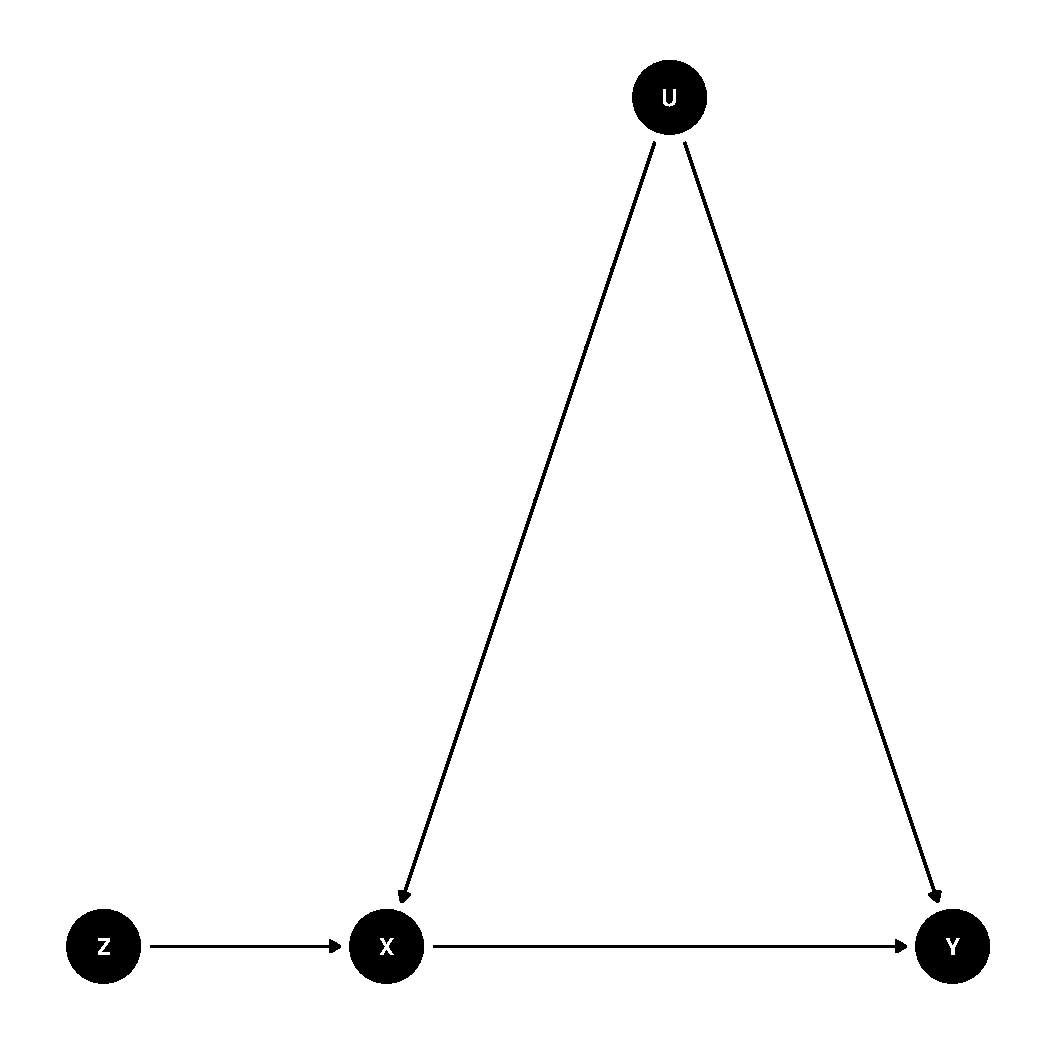
\includegraphics[width=0.5\linewidth]{data/introduction/figures/mrdag1} 

}

\caption[Directed acyclic graph of the Mendelian randomization principle]{\textbf{Directed acyclic graph of the Mendelian randomization principle}. Z = instrumental variable; X = exposure; Y = outcome; U = confounders of the exposure-outcome association.}\label{fig:introduction-figure-mr-dag}
\end{figure}
Additional assumptions based on homogeneity, monotonicity, and effect modification are also present. The homogeneity assumption assumes the association between the IV and exposure or the effect of the exposure on the outcome is homogeneous. That is, the association or the effect is the same for all individuals in the population. Monotonicity can be deterministic or stochastic. Deterministic monotonicity assumes that the effect of the IV is consistent in all individuals of the population. That is, the effect of the IV does not increase the exposure in one group and decrease it in another. Stochastic monotonicity assumes deterministic monotonicity conditional on confounders.

\par

Based up-on Mendel's laws of inheritance, MR relies on the assumption that genetic variants are unlikely to be associated with one another (outside of linkage disequilibrium (LD)) or with environmental factors. Deviation from which would mean an uneven distribution of alleles across a population. Consideration in MR analyses should therefore also be given to dynastic effects, population structure, and assortative mating as these sources are the most likely ways in which the second MR assumption can be violated. Within-family MR is one method that can be used to estimate the causal effect in these situations\textsuperscript{\protect\hyperlink{ref-Hartwig2018}{363},\protect\hyperlink{ref-Brumpton2019}{364}}.

\par

Dynastic effects, a form of confounding, are a consequence of traits transmitted across generations which then influence the causal effect estimate\textsuperscript{\protect\hyperlink{ref-Brumpton2019}{364},\protect\hyperlink{ref-Sanderson2019}{365}}. That is, the parental genotype directly effects the offspring phenotype. For example, the effect of BMI on CVD may be biased by the IVs for BMI being correlated across parent and offspring and the effect of maternal BMI on offspring development, which has an effect on future CVD. Simply put, if the parent has a high BMI that could effect the environment the child is brought up in which would then be associated with the childs risk of developing CVD. In this instance, the second MR assumption would be violated. Within family studies are proposed, and simulations have shown, to overcome some of the consequences of dynastic effects\textsuperscript{\protect\hyperlink{ref-Brumpton2019}{364},\protect\hyperlink{ref-Sanderson2019}{365}}.

\par

Population structure is a result of allele frequencies differing across geographic regions. This would also violate the second MR assumption. In MR analyses it is assumed that latent structure is accounted for in the GWAS in which the IVs are discovered\textsuperscript{\protect\hyperlink{ref-Haworth2019}{366}}. As the sample sizes of GWAS has increased, the potential for subtle effects of population structure have been observed\textsuperscript{\protect\hyperlink{ref-Haworth2019}{366},\protect\hyperlink{ref-Berg2019}{367}}. Though one can restrict analyses to homogeneous groups, use principal components, and perform within family studies to examine and mitigate the effects of population stratification, biases (e.g.~sampling bias) may still remain\textsuperscript{\protect\hyperlink{ref-Brumpton2019}{364}}.

\par

Assortative mating is the principle by which partners select one another based on a particular phenotype. This is either cross-trait (one trait selecting for another trait) or single-trait (one trait selecting for the same trait). MR results can be biased by both types of assortative mating, even when the phenotypes of interest are not those which influenced the mating\textsuperscript{\protect\hyperlink{ref-Hartwig2018}{363}}. It is currently difficult to test and account for the effects of assortative mating, but within-family studies have shown some promise in this regard\textsuperscript{\protect\hyperlink{ref-Brumpton2019}{364}}.

\par

Formal assessment of the exclusion restriction assumption is not possible, however a number of methods have been developed to assess potential violation of this assumption. The most widely used of these methods are MR-Egger, weighted mode, and weighted median. MR-Egger provides an estimate of unbalanced/directional horizontal pleiotropy via the intercept of a linear regression of the SNP-exposure and SNP-outcome association. In the presence of pleiotropy the intercept will bias away from the origin. MR-Egger gives consistent estimates when 100\% of genetic instruments are invalid\textsuperscript{\protect\hyperlink{ref-Bowden2015}{368}}. The weighted median is complimentary to MR-Egger but does not rely on the ``instrument strength independent of direct effect'' (InSIDE) assumption. It calculates the median of an empirical distribution of the causal effect estimates weighted for precision. It provides consistent estimates when at least 50\% of the weight comes from valid genetic instruments and as long as no one genetic instrument contributes \textgreater{} 50\% of the weight\textsuperscript{\protect\hyperlink{ref-Burgess2017a}{369}}. The weighted mode assumes the true causal effect is the most common effect, it is robust when the majority of effect estimates are derived from valid instruments\textsuperscript{\protect\hyperlink{ref-Hartwig2017}{370}}.

\par

Canalization, whereby what would otherwise be developmentally deleterious genetic effects are nullified by compensatory mechanisms, is broadly equivalent to non-adherence in an RCT. Any effects of canalization would attenuate effect sizes\textsuperscript{\protect\hyperlink{ref-Smith2004}{357}}, however there are currently no methods to detect its presence in an MR context. The effects of canalization are unlikely to be present in MR studies which utilise maternal genotypes for environmental exposures of the offspring such as during gestation\textsuperscript{\protect\hyperlink{ref-Smith2010}{371}}. For complex traits, it is possible that canalization occurs at the level of the system rather than at the gene level\textsuperscript{\protect\hyperlink{ref-Geiler-Samerotte2019}{372}}. As such, any outcome of a genetic mutation in regards to its role in the canal would likely be unpredictable. Though being aware of the underlying biology can inform analyses, it is not currently possible to account for for canalization in MR analyses.

\par

In both one-sample and two-sample MR, IVs are often obtained from external GWAS. Increasingly, these are large and well-powered GWAS able to identify ever increasing numbers of SNPs associated with complex traits such as BMI\textsuperscript{\protect\hyperlink{ref-Speliotes2010}{45},\protect\hyperlink{ref-Locke2015}{48},\protect\hyperlink{ref-Shungin2015}{49},\protect\hyperlink{ref-Yengo2018}{53},\protect\hyperlink{ref-Pulit2019}{54}}. As power has increased, the ability to detect SNPs with smaller effects which explain ever smaller proportions of variance in BMI has increased\textsuperscript{\protect\hyperlink{ref-Yengo2018}{53}}. This holds potential considerations in regards to population structure and the effects of an omnigenic model\textsuperscript{\protect\hyperlink{ref-Boyle2017}{29}}. As discussed, population structure was thought to have been an issue in smaller studies and could be accounted for by adjustment. However, well-powered studies have shown both latent structure\textsuperscript{\protect\hyperlink{ref-Haworth2019}{366},\protect\hyperlink{ref-Berg2019}{367}} and an inability to perform adequate adjustment\textsuperscript{\protect\hyperlink{ref-Sohail2019}{373}}. This has potential implications, not only for the effect sizes of associated SNPs but also for the identification of SNPs associated with the trait\textsuperscript{\protect\hyperlink{ref-Sohail2019}{373}}. For example, a poorly or un-adjusted GWAS could identify SNPs associated with population differences rather than the trait of interest.

\par

When MR was first described, traits were instrumented mostly using a small number number of well characterised SNPs. These SNPs would explain a small amount of trait variance, but the underlying biology was understood. More recently, GWAS are, and have been, able to identify large numbers of SNPs which explain ever larger proportions of trait variance. With this added power however comes a more complex instrument with many potential biological mechanisms linking SNPs to the trait. In an omnigenic model, variance in a trait of interest is not solely a result of directly related genes (core-genes). Rather, all genes expressed in relevant cell types have an effect, however small, on the trait of interest\textsuperscript{\protect\hyperlink{ref-Boyle2017}{29}}. These peripheral genes, which have no obvious direct link to the trait of interest, are mostly in non-coding regions with regulatory functions\textsuperscript{\protect\hyperlink{ref-Liu2019}{67}}. Given that variants associated with complex traits are dispersed widely across the genome\textsuperscript{\protect\hyperlink{ref-Liu2019}{67}} and that assigning a link between any particular SNP and an individual gene is difficult\textsuperscript{\protect\hyperlink{ref-GTEx2013}{68}}, variants associated with complex traits likely implicate many genes with the trait. Because many of these will be peripheral genes (not core genes), they will ultimately have functions on other traits, which in an MR context may include the outcome and thus violate the exclusion restriction assumption.

\par

Additional considerations include random measurement error (random measurement in the exposure will bias the causal estimate towards the null, and increase the standard error of the causal effect estimate if in the outcome), Winner's curse (whereby discovery studies identify larger effects than those in replication studies), collider bias (conditioning on a variable by adjustment, restriction, or sampling can induce an association between \(X\) and \(Y\), biasing the estimate either away or towards the null), overlapping samples (specific to two-sample MR, where the exposure and outcome data are obtained from samples with shared individuals), and vertical pleiotropy (the IV influences multiple traits, including the exposure, on the same pathway linking the exposure and outcome). Unlike the other considerations, vertical pleiotropy does not necessarily bias MR results rather it highlights potential intermediates.

\par

Both one- and two-sample MR can be extended to investigate intermediates that sit on the causal pathway between an exposure and outcome. Mediation analysis in MR is discussed in detail elsewhere\textsuperscript{\protect\hyperlink{ref-Carter2020}{374}} and can be achieved using two-step\textsuperscript{\protect\hyperlink{ref-Relton2012}{375}}/network MR\textsuperscript{\protect\hyperlink{ref-Burgess2015}{359}} and multivariable MR\textsuperscript{\protect\hyperlink{ref-Sanderson2018}{376}} (MVMR). Briefly, mediation analysis is interested in identifying the total effect, the direct effect, and the indirect effect; where all act in the same direction, the proportion of the total effect explained by the mediator (proportion mediated) can be calculated\textsuperscript{\protect\hyperlink{ref-VanderWeele2016}{377}}. The total effect is the effect of the exposure on the outcome through all mediated pathways; the direct effect is the effect of the exposure on the outcome through all mediated pathways that are not the pathway of interest; the indirect effect is the effect of the exposure on the outcome through the mediator of interest. These analyses are predicated on the following assumptions: (i) that there is a causal effect of the exposure on the mediator and of the mediator on the outcome; (ii) that there is no confounding between exposure, mediator, and outcome; (iii) that there are no intermediate confounders; (iv) that there is no interaction between the exposure and mediator\textsuperscript{\protect\hyperlink{ref-VanderWeele2016}{377}}.

\par

In two-step MR (Figure \ref{fig:introduction-figure-mr-dag2}), the indirect effect is calculated by multiplying the effect of the exposure on the intermediate and the effect of the intermediate on the outcome. The three core MR assumptions (and all previous considerations) must still be met and also extended: (i) the IV (\(Z1\) \& \(Z2\)) must be robustly associated with the exposure or intermediate only (\(X\) and \(M\)), (ii) the IV for the exposure (\(Z1\)) and intermediate (\(Z2\)) must not be associated with measured or unmeasured confounders (\(U\)), (ii) the IV for the exposure (\(Z1\)) must not be associated with the intermediate (\(M\)) or the outcome (\(Y\)) other than through the exposure (\(X\)), and the intermediate IV (\(Z2\)) must not be associated with the exposure, and only with the outcome (\(Y\)) through the intermediate. No interaction between exposure and intermediate is also assumed. Two-step MR has been used\textsuperscript{\protect\hyperlink{ref-Varbo2015}{378}--\protect\hyperlink{ref-Marouli2019}{380}} and combined with MVMR\textsuperscript{\protect\hyperlink{ref-Carter2019}{381}} to gain better insight into disease aetiology, but is not strictly speaking mediation analysis.

\par




\begin{figure}

{\centering 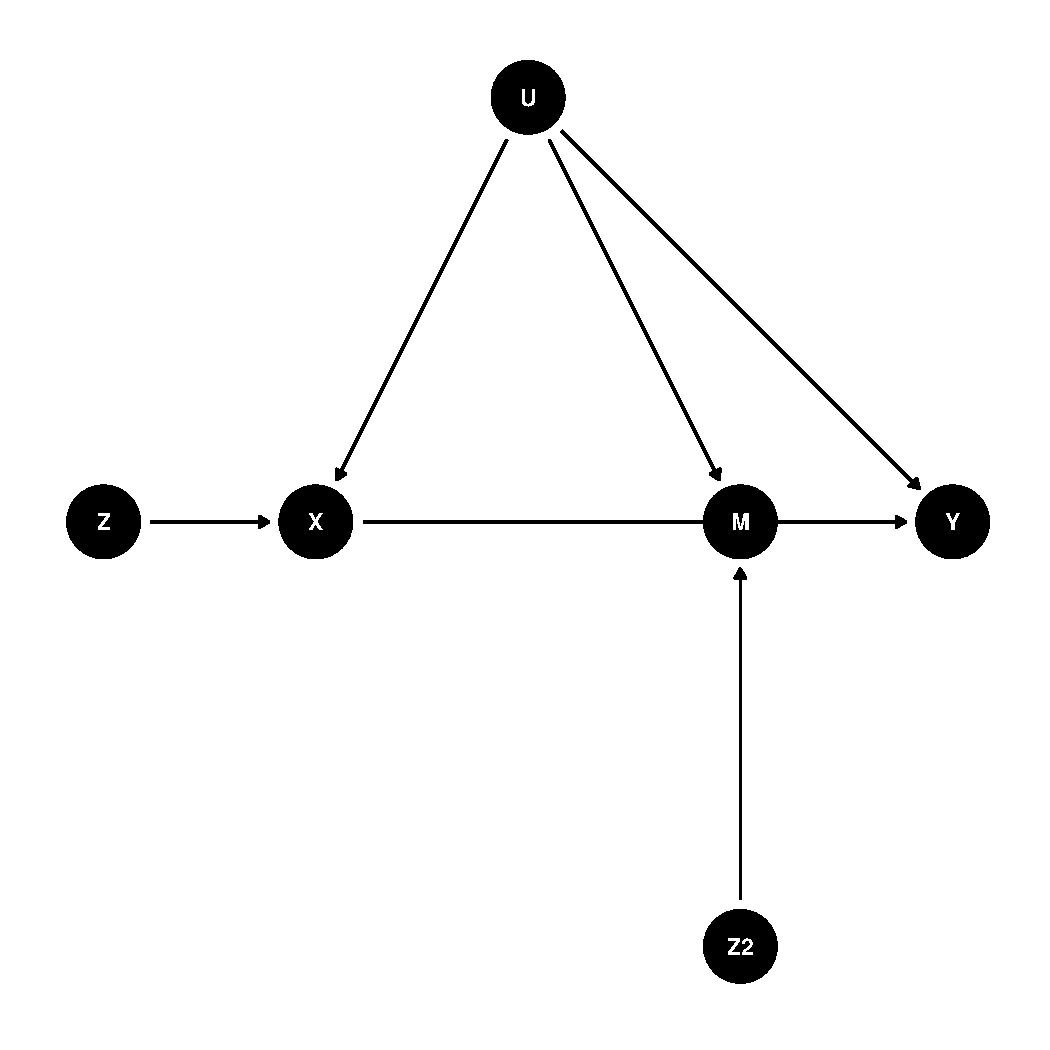
\includegraphics[width=0.5\linewidth]{data/introduction/figures/mrdag2} 

}

\caption[Directed acyclic graph of the two-step Mendelian randomization principle]{\textbf{Directed acyclic graph of the two-step Mendelian randomization principle}. Z = instrumental variable; X = exposure; M = intermediate; U = confounders; Z2 = instrumental variable for M; Y = outcome.}\label{fig:introduction-figure-mr-dag2}
\end{figure}
MVMR is a form of mediation analysis which allows for the causal effects of multiple exposures on an outcome to be estimated\textsuperscript{\protect\hyperlink{ref-Sanderson2018}{376}} (Figure \ref{fig:introduction-figure-mr-dag3}). The effect of each exposure is estimated conditional on the other exposures and thus provides a direct estimate of the effect. Figure \ref{fig:introduction-figure-mr-dag3} shows a simplified MVMR model with two exposures (\(X1\) and \(X2\)). The indirect effect is estimated by subtraction of the direct effect from the total effect. The total effect is calculated using univariable MR. As with two-step MR, no interaction between exposure and intermediate is assumed. Though a new approach, and still subject to the same assumptions as with two-step and univariable MR, MVMR has shown promise in elucidating underlying aetiology of complex traits\textsuperscript{\protect\hyperlink{ref-Carter2019}{381}--\protect\hyperlink{ref-Johnson2019}{384}}.

\par




\begin{figure}

{\centering 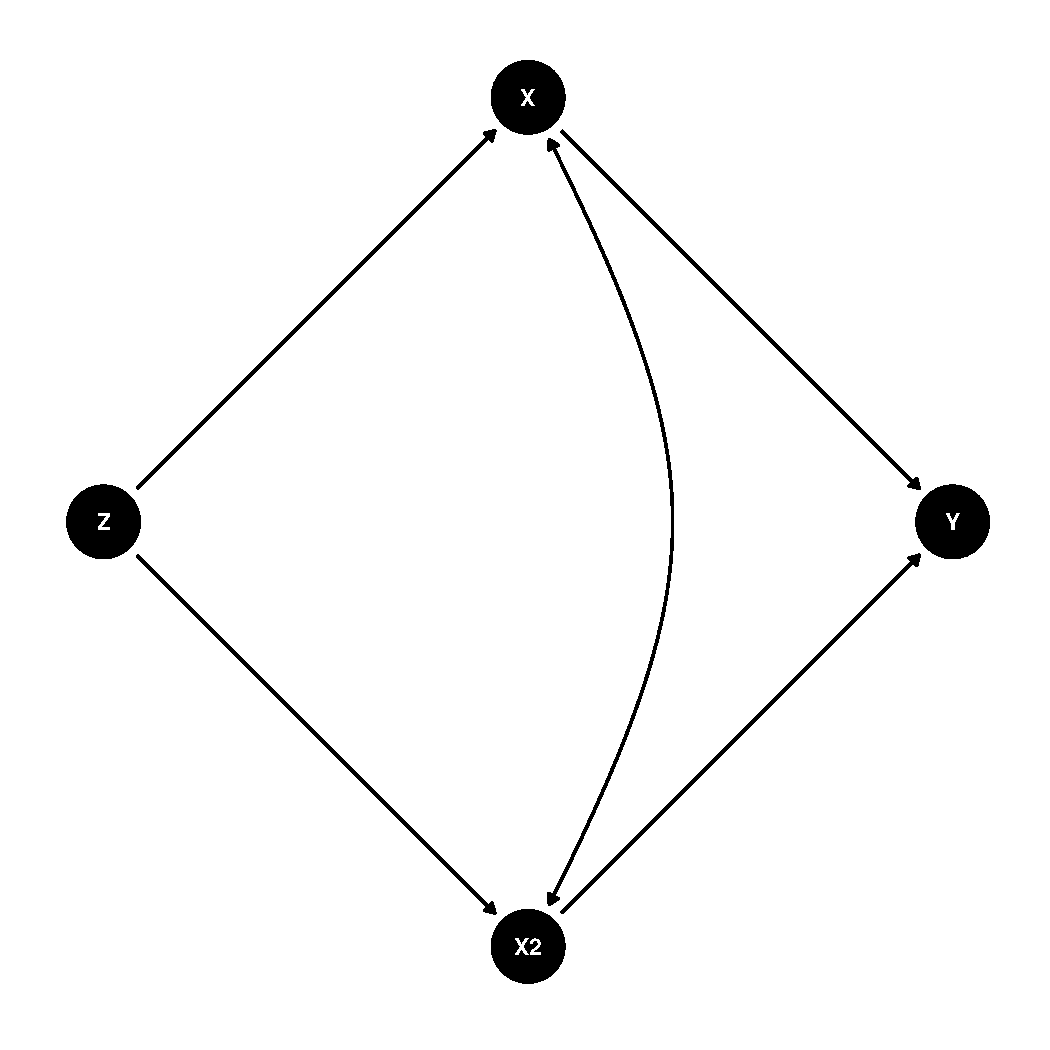
\includegraphics[width=0.5\linewidth]{data/introduction/figures/mrdag3} 

}

\caption[Directed acyclic graph of the multivariable Mendelian randomization principle using two exposures]{\textbf{Directed acyclic graph of the multivariable Mendelian randomization principle using two exposures}. Z = instrumental variables associated with one or more of the exposures; X1 = exposure; X2 = second exposure (mediator); Y = outcome; U = confounders.}\label{fig:introduction-figure-mr-dag3}
\end{figure}
Though two-step MR was devised with epigenetic mechanisms in mind\textsuperscript{\protect\hyperlink{ref-Relton2012}{375}} and MVMR has shown promise investigating metabolic intermediates\textsuperscript{\protect\hyperlink{ref-Richardson2019}{383}}, their application to large omic data sets is yet to be shown. An alternative approach is to look for overlapping signals. In this regard, the effect of the exposure on the candidate intermediate and the effect of the candidate intermediate on the outcome are ranked in terms of their effects. A candidate intermediate is considered if it ranks highly in both analyses\textsuperscript{\protect\hyperlink{ref-Guida2021}{385}}.

\par

\hypertarget{previous-work}{%
\section{Previous work}\label{previous-work}}

Metabolites have been a focus of research for some time, with many population-based studies collecting data on traditional biomarkers (e.g., glucose and cholesterol). As technologies such as MS and NMR have progressed, the number of metabolites able to be studied at scale has increased. There is evidence for an association between adiposity and metabolites\textsuperscript{\protect\hyperlink{ref-Wurtz2014}{286},\protect\hyperlink{ref-Cirulli2019}{287},\protect\hyperlink{ref-Moore2014}{345},\protect\hyperlink{ref-SantosFerreira2017}{386}--\protect\hyperlink{ref-Rangel-Huerta2019}{395}}. These studies show associations between BMI and metabolites vary between sexes and over time\textsuperscript{\protect\hyperlink{ref-Wurtz2014}{286},\protect\hyperlink{ref-OKeeffe2020}{390}}; associations are stronger\textsuperscript{\protect\hyperlink{ref-Wurtz2014}{286},\protect\hyperlink{ref-OKeeffe2020}{390}} and appear earlier in men\textsuperscript{\protect\hyperlink{ref-OKeeffe2020}{390}}. There is also evidence for associations with metabolites and BF\textsuperscript{\protect\hyperlink{ref-OKeeffe2020}{390}}, WC\textsuperscript{\protect\hyperlink{ref-Stevens2020}{389},\protect\hyperlink{ref-Bachlechner2016}{394}}; WHR\textsuperscript{\protect\hyperlink{ref-Wulaningsih2019}{391}}, and visceral adipose tissue\textsuperscript{\protect\hyperlink{ref-Neeland2019}{393},\protect\hyperlink{ref-Boone2019}{396}}. These large scale metabolomics studies have also highlighted numerous associations between metabolites and other outcomes, from type 2 diabetes\textsuperscript{\protect\hyperlink{ref-Ahola-Olli2019}{397}} and CHD\textsuperscript{\protect\hyperlink{ref-Cavus2019}{398}}, to depression\textsuperscript{\protect\hyperlink{ref-Bot2020}{399}}, hypertension\textsuperscript{\protect\hyperlink{ref-Onuh2020}{400}}, and more\textsuperscript{\protect\hyperlink{ref-Bos2021}{1},\protect\hyperlink{ref-Gowda2008}{401}--\protect\hyperlink{ref-Volani2021}{408}}. Evidence also suggests that metabolites can distinguish between cancers and adenomas\textsuperscript{\protect\hyperlink{ref-Kovesdy2017}{184}}.

\par

Few studies have investigated the explicit link between adiposity, metabolites, and disease outcomes\textsuperscript{\protect\hyperlink{ref-Cirulli2019}{287},\protect\hyperlink{ref-Ho2016}{409}--\protect\hyperlink{ref-Cheng2012}{411}}. Evidence suggests that BMI is linked to changes in specific metabolites and metabolite classes, and that several of these are subsequently associated with, or predictors of, later health outcomes such as insulin resistance\textsuperscript{\protect\hyperlink{ref-Newgard2009}{410}}. However, these studies\textsuperscript{\protect\hyperlink{ref-Cirulli2019}{287},\protect\hyperlink{ref-Ho2016}{409}--\protect\hyperlink{ref-Cheng2012}{411}} have three main limitations: (i) they involved a small number of individuals (N = 140-1,761), (ii) used a single measure of adiposity (BMI), or (iii) used methods that are unable to establish causality.

\par

Evidence from MR analyses suggests numerous associations between adiposity and metabolites\textsuperscript{\protect\hyperlink{ref-Wurtz2014}{286},\protect\hyperlink{ref-Fall2013}{412}--\protect\hyperlink{ref-Bull2020}{415}}. Although many studies have focussed on curated lists of metabolites, in larger analyses, fewer associations are found than with observational analyses\textsuperscript{\protect\hyperlink{ref-Wurtz2014}{286},\protect\hyperlink{ref-Liu2017c}{414},\protect\hyperlink{ref-Hsu2020}{416}}. MR studies have revealed this relationship to be a complex network of cause and effect, with metabolites being causes of, or effects of, adiposity\textsuperscript{\protect\hyperlink{ref-Hsu2020}{416}}. Work by Hsu et al.~(2020)\textsuperscript{\protect\hyperlink{ref-Hsu2020}{416}} found that associations with adiposity were mechanistically different based on whether a metabolite was identified as a cause or as an effect of adiposity. The causal relationship between metabolites and outcomes is much less well studied, likely due to challenges in instrumentation -- few metabolites have been associated with robust and strong instruments. A number of associations have been identified between metabolites and health outcomes, including type 2 diabetes\textsuperscript{\protect\hyperlink{ref-Liu2017c}{414},\protect\hyperlink{ref-Porcu2021}{417}}, fasting glucose\textsuperscript{\protect\hyperlink{ref-Liu2017c}{414},\protect\hyperlink{ref-Porcu2021}{417}}, colorectal cancer\textsuperscript{\protect\hyperlink{ref-Bull2020}{415}}, CHD\textsuperscript{\protect\hyperlink{ref-Burgess2016a}{418}}, and more\textsuperscript{\protect\hyperlink{ref-Lord2021}{419}--\protect\hyperlink{ref-Qin2020}{422}}.

\par

Few studies have looked causally at the pathways linking adiposity with metabolites and outcomes. Xu et al.~(2017)\textsuperscript{\protect\hyperlink{ref-Xu2017}{379}} performed a two-step two-sample MR of BMI and HDL, low density lipoprotein cholesterol (LDL), and triacylglycerides on CHD, but did not find evidence for a pathway effect. Recently, Bull et al.~(2020)\textsuperscript{\protect\hyperlink{ref-Bull2020}{415}} used MR to investigate the effects of BMI and WHR with 123 metabolites on colorectal cancer. Metabolites associated with BMI and/or WHR (N = 104) were used in univariable and MVMR to establish associations with colorectal cancer. Intermediate density lipoproteins (IDL) and very large density lipoproteins (VLDL) showed consistent directions, both were increased by BMI and WHR, and both increased CRC (distal colon cancer) risk. In MVMR analysis, associations for BMI and WHR were not attenuated after adjusting for either metabolites, suggesting these metabolites may not play an intermediate role in the relationship between adiposity and colorectal cancer.

\par

There is evidence of a causal effect of adiposity on metabolites, of metabolites on diseases, and of adiposity on diseases. However, only the study by Bull et al\textsuperscript{\protect\hyperlink{ref-Bull2020}{415}} has investigated the pathways linking adiposity with metabolites and outcomes causally. Their analyses were likely subject to weak instrument bias however. Future analyses require more detailed metabolomic measures, with large sample sizes able to identify strong and robust instruments in order to fully address this question.

\par

\hypertarget{aims}{%
\section{Aim and objectives}\label{aims}}

Adiposity is a global health concern. Many of the consequences of adiposity have been characterized but the underlying aetiology is not well understood. Adipose tissue is a prolific signalling organ with systemic effects, some of which are likely to affect the metabolome. Individual metabolites have been associated with many diseases but the complexity of the network makes these analyses difficult. MR studies provide an opportunity to investigate and disentangle the complex relationship between exposure, intermediate, and outcome. These studies must be approached carefully given the interrelatedness of metabolites. In light of these considerations' this thesis aims to: \textbf{\emph{Identify metabolites that sit on the causal pathway between adiposity and disease}}. In order to achieve this aim, this thesis will investigate the following objectives:
\begin{enumerate}
\def\labelenumi{\arabic{enumi}.}
\tightlist
\item
  Perform a systematic review and meta-analysis (Chapter \ref{systematic-review}) of all MR studies in which a measure of adiposity was used as an exposure, identifying diseases that will guide later analyses (Chapter \ref{mediation}).

  \par
\item
  Produce a visualisation tool that enables global overview of metabolite results (Chapter \ref{visualisation}).

  \par
\item
  Identify metabolites associated with adiposity using observational epidemiological analysis with individual level data (Chapter \ref{observational}).

  \par
\item
  Identify metabolites that may be causally impacted by adiposity using MR (Chapter \ref{MR}).

  \par
\item
  Identify associations between adiposity-associated metabolites (Chapter \ref{observational} and \ref{MR}) and adiposity-associated outcomes (Chapter \ref{systematic-review}) using univariable and MVMR (Chapter \ref{mediation})
\end{enumerate}
\newpage

\hypertarget{systematic-review}{%
\chapter{Systematic review: What has the application of Mendelian randomization told us about the causal effect of adiposity and health outcomes?}\label{systematic-review}}

\hypertarget{chapter-summary-1}{%
\section*{Chapter Summary}\label{chapter-summary-1}}
\addcontentsline{toc}{section}{Chapter Summary}

This Chapter details a systematic review and meta-analysis of 173 Mendelian randomization (MR) articles investigating the effects of adiposity on over 300 different outcomes. In Chapter \ref{introduction}, focus was given to the underlying literature around adiposity, what adipose tissue is, why in excess this can be detrimental to health, what observational studies have taught us about adiposity, and potential mechanisms for relationships between adiposity and disease. Here, the focus is on the causal effects of adiposity and what Mendelian randomization studies have revealed about the relationships between adiposity and disease. Results reveal the broad effect of adiposity on many health outcomes, with meta-analyses highlighting a number of outcomes (e.g., endometrial cancer, colorectal cancer, cardiovascular disease) for follow up analysis in Chapter \ref{mediation}. This work was pre-registered on \href{https://www.crd.york.ac.uk/prospero/display_record.php?ID=CRD42018096684}{PROSPERO}\textsuperscript{\protect\hyperlink{ref-Lee2018}{104}}.

\par

\newpage

\hypertarget{SR-intro}{%
\section{Introduction}\label{SR-intro}}

Observational studies have indicated that adiposity is strongly associated with all-cause and cause specific mortality\textsuperscript{\protect\hyperlink{ref-Pischon2008}{82},\protect\hyperlink{ref-Flegal2013}{86}--\protect\hyperlink{ref-Elagizi2018}{88},\protect\hyperlink{ref-Jenkins2018}{100}--\protect\hyperlink{ref-Bigaard2004}{105}}, and numerous risk factors and diseases\textsuperscript{\protect\hyperlink{ref-Lee2018}{104},\protect\hyperlink{ref-Barberio2019}{107}--\protect\hyperlink{ref-Mathew2008}{141},\protect\hyperlink{ref-McGill2002}{148}--\protect\hyperlink{ref-Lavie2017}{152},\protect\hyperlink{ref-Kurth2002}{154}--\protect\hyperlink{ref-Rost2001}{156},\protect\hyperlink{ref-Festa2001}{159}--\protect\hyperlink{ref-Stryjecki2011}{169}}

\vspace*{-1em}

\noindent\textsuperscript{,}\textsuperscript{\protect\hyperlink{ref-Al-Goblan2014}{171},\protect\hyperlink{ref-Kovesdy2017}{184}--\protect\hyperlink{ref-Kramer2016}{192},\protect\hyperlink{ref-Fabbrini2010}{196}--\protect\hyperlink{ref-Cornier2008}{201},\protect\hyperlink{ref-Donnelly2005}{203},\protect\hyperlink{ref-OBrien2017}{205}--\protect\hyperlink{ref-Alosco2014}{218},\protect\hyperlink{ref-Thaler2010}{222},\protect\hyperlink{ref-MyersJr2010}{223},\protect\hyperlink{ref-Zammit2010}{230}--\protect\hyperlink{ref-Beuther2007}{234},\protect\hyperlink{ref-Rodrigo2007}{236}--\protect\hyperlink{ref-Stang2016}{248},\protect\hyperlink{ref-Sharp2019}{250}--\protect\hyperlink{ref-Ehrmann2006}{256},\protect\hyperlink{ref-OrioJr2004}{258}--\protect\hyperlink{ref-Athukorala2010}{267},\protect\hyperlink{ref-Belbasis2016}{270},\protect\hyperlink{ref-Stothard2009}{273}--\protect\hyperlink{ref-Martyn2008}{276},\protect\hyperlink{ref-Ye2013}{280},\protect\hyperlink{ref-Wilkin2001}{282},\protect\hyperlink{ref-Corbin2018}{283},\protect\hyperlink{ref-Kahn2001}{285}--\protect\hyperlink{ref-Figarska2020}{292}}. This includes the most common diseases, such as cardiovascular disease (CVD)\textsuperscript{\protect\hyperlink{ref-Lee2018}{104},\protect\hyperlink{ref-Dobbelsteyn2001}{108},\protect\hyperlink{ref-Yusuf2005}{109},\protect\hyperlink{ref-Romero-Corral2010}{117},\protect\hyperlink{ref-Paul2006}{134}--\protect\hyperlink{ref-Lavie2017}{152},\protect\hyperlink{ref-Kurth2002}{154}--\protect\hyperlink{ref-Rost2001}{156}} and many cancers\textsuperscript{\protect\hyperlink{ref-Lee2018}{104},\protect\hyperlink{ref-Barberio2019}{107},\protect\hyperlink{ref-Bhaskaran2014}{120}--\protect\hyperlink{ref-Heo2021}{133}}, along with common risk factors such as high blood pressure\textsuperscript{\protect\hyperlink{ref-Mathew2008}{141},\protect\hyperlink{ref-Wurtz2014}{286}}. See Chapter \ref{introduction} Section \ref{introduction-morbidities} for more detail.

\par

As discussed in Chapter \ref{introduction} Section \ref{mendelian-randomization}, observational studies hold a number of limitations that can not easily be overcome, e.g., confounding and reverse causation. These limitations can lead to biased results\textsuperscript{\protect\hyperlink{ref-CCGC2011}{157},\protect\hyperlink{ref-Timpson2005}{179},\protect\hyperlink{ref-Batty1999}{350}--\protect\hyperlink{ref-Yarmolinsky2018}{353}} and, although an observational study may identify an association between two traits, this does not mean that one trait causes the other; they may be correlated because of shared causes, for instance. Furthermore, in observational studies, it is difficult to obtain the causal direction of effect as the temporal sequence is generally unknown\textsuperscript{\protect\hyperlink{ref-Batty1999}{350}}. Ideally randomised controlled trials (RCTs) would be conducted to aid our understanding and identify causal effects, however these are costly, time consuming, and can be unethical given the assumption that adiposity is detrimental to health. Mendelian randomization (MR) analyses provide a method of obtaining causal effects outside of RCTs\textsuperscript{\protect\hyperlink{ref-DaveySmith2003}{356}}. By using germline genetic variants, which are randomly assigned and fixed at conception, randomization analogous to an RCT can be achieved (See Chapter \ref{introduction} Section \ref{mendelian-randomization}). There has been a rise in MR studies published in the years since it was first widely reported on in 2003\textsuperscript{\protect\hyperlink{ref-DaveySmith2003}{356}}.

\par

Systematic reviews enable global overview of the literature and provide avenues for hypothesis generation. In combination with meta-analyses, systematic reviews can be used as a method for improved causal inference as pooled estimates can be more precise than estimates from individual studies\textsuperscript{\protect\hyperlink{ref-Deeks2019}{423}}. The MR literature has not been systematically appraised with respect to the causal effect of the effect of adiposity on health outcomes. Here, a systematic review and meta-analysis are presented and will be used to inform downstream analyses within this thesis, namely selecting outcomes for which adiposity is most relevant and to test associations with adiposity-related metabolic intermediates (Chapter \ref{mediation}).

\par

\hypertarget{SR-methods}{%
\section{Methods}\label{SR-methods}}

\hypertarget{data-sources-and-search-strategy}{%
\subsection{Data sources and search strategy}\label{data-sources-and-search-strategy}}

EMBASE and MEDLINE were searched from inception (EMBASE = 1974; MEDLINE = 1946) until February 18th 2019 using detailed search strategies including free text and controlled vocabulary terms. The full search strategy is available on \href{https://github.com/mattlee821/000_thesis/blob/master/index/data/SR/data/search_strategy.pdf}{GitHub}. The pre-print service, bioRxiv, was also searched from inception (November 2013) until February 18th 2019. However, due to the limited search functionality and inability to include Boolean operators (`AND', `OR', `NOT') in bioRxiv searches, a restricted search strategy using four free text terms in four independent searches was used: `Mendelian randomization', `Mendelian randomisation', `causal inference', and `causal analysis'. `Adiposity' and related search terms were not used as this would have identified a much larger body of work, and given Boolean operators could not be used, filtering this larger body for studies which performed MR would have been more time consuming than filtering MR studies which used adiposity as an exposure.

\par

The search strategy included synonyms for both adiposity and MR terms. For adiposity measures, this was to ensure searches returned all possible instances in which a measure of adiposity was used. For MR, synonyms were used as the term `Mendelian randomization' has only been formalised recently and many early studies would have either been unaware they were performing an instrumental variable (IV) analysis or would have called the method something else.

\par

\hypertarget{study-selection}{%
\subsection{Study selection}\label{study-selection}}

Articles returned through the searches of EMBASE and MEDLINE were downloaded as \texttt{.ris} files and imported into EndNote (version X8.2; Clarivate Analytics). De-duplication of articles identified in the EMBASE and MEDLINE searches was based on pagination identifiers described in detail elsewhere\textsuperscript{\protect\hyperlink{ref-Bramer2016}{424}}. Articles returned from bioRxiv were imported into Mendeley using the Mendeley Google Chrome extension and de-duplication performed using the Mendeley de-duplication function. After de-duplication, the titles and abstracts of all remaining articles from EMBASE, MEDLINE, and bioRxiv had their titles and abstracts screened by two independent reviewers (myself and Luke A Mcguinness) using Rayyan\textsuperscript{\protect\hyperlink{ref-Ouzzani2016}{425}}. Each reviewer screened all articles and discrepancies at this stage were resolved through discussion between the two reviewers. Studies from EMBASE, MEDLINE, and bioRxiv meeting the pre-defined inclusion criteria (see below) were combined and, in instances where the bioRxiv study had been published and this was identified in either the EMBASE or MEDLINE search, the bioRxiv version of the study was excluded. The full texts of all studies that met inclusion criteria were screened by the two reviewers.

\par

For title and abstract screeening and for full text screening, articles must have met the following pre-defined inclusion criteria:
\begin{enumerate}
\def\labelenumi{\arabic{enumi}.}
\tightlist
\item
  Be written in English.
\item
  Be available in full text (or in the case of conference abstracts, the authors must be contactable to obtain the relevant data).
\item
  Be published in a peer-reviewed journal or bioRxiv.
\item
  Use MR methodology to investigate the causal effect of adiposity on any outcome.
  \begin{enumerate}
  \def\labelenumii{\alph{enumii}.}
  \tightlist
  \item
    Adiposity was considered to be any measure which aimed to assess the amount of adipose tissue an individual possessed.
  \item
    If a study focussed on adiposity alongside other exposures, the effect of each adiposity measure was reported separately if available. If it was not available the joint effect was reported.
  \item
    Articles in which an MR approach was used but not explicitly called `Mendelian randomization' was included. More specifically, any study in which genetic variants are used as instrumental variables or the direct association between a genetic variant and outcome was employed was eligible, provided it met the other inclusion criteria.
  \end{enumerate}
\end{enumerate}
\hypertarget{data-extraction}{%
\subsection{Data extraction}\label{data-extraction}}

In the first instance, data extraction was performed by nine reviewers (See Contributions), with articles split evenly between them, using a data extracton form (\href{https://github.com/mattlee821/000_thesis/blob/master/index/data/SR/data/data_extraction.xlsx}{GitHub}) and data extraction manual (\href{https://github.com/mattlee821/000_thesis/blob/master/index/data/SR/data/data_extraction_manual.docx}{GitHub}) which I created. Once all articles had been reviewed, two reviewers (See Contributions) extracted data on all articles they did not review in the first instance. The same two reviewers then checked all extracted data for discrepancies, which were resolved through a third review of individual articles and subsequent discussion.

\par

In some cases, articles included in the data extraction contained more than one relevant MR analysis. As such, the words ``study'' and ``studies'' refer to the MR analysis and analyses within an article. The following data were extracted from each of the studies from all of the contributing articles: exposure(s), outcome(s), study design and sample characteristics, genetic variant and IV selection, MR methodology, sensitivity analysis, and causal estimates. Where relevant data was not reported by the article, ``Not discussed'' was entered into the data extraction form.

\par

Once data extraction was completed, three additional columns were added to summarise the type of outcome being studied: column 1 (``outcome'') was used as a general categorisation of all outcomes across articles (e.g., the outcome ``ER- breast cancer'' would have the value ``breast cancer''); column 2 (``outcome info'') reported the outcome-specific information that distinguished outcomes within categories defined in column 1 (e.g., column 2 would contain the value ``oestrogen recepter negative (ER-) breast cancer'' for the same breast cancer example); and column 3 (``outcome group'') categorised outcomes more generally than values defined in column 1 (e.g., the breast cancer example would be categorised as ``cancer''). Outcome categories were assigned based on prior biological knowledge and aimed to collapse the large number of outcomes. This could be achieved differently for some outcomes, for example smoking could go in a ``respiratory'' category or a ``behavioural'' category. Where there were few outcomes to make a category, they were grouped into an ``other'' category. This will include outcomes such as mortality, disease counts, epigenetic marker, etc.

\par

\hypertarget{quality-assessment}{%
\subsection{Quality assessment}\label{quality-assessment}}

There is currently no risk of bias tool to assess the quality of MR articles. Because of this, some reviews have not reported on the quality of MR studies\textsuperscript{\protect\hyperlink{ref-Pingault2016}{426},\protect\hyperlink{ref-Storm2020}{427}}. However, more recent studies have begun to investigate quality, either by using pre-existing risk of bias tools specific to other areas or by creating their own assessment tool\textsuperscript{\protect\hyperlink{ref-Kuzma2018}{428}--\protect\hyperlink{ref-Grau-Perez2019}{439}}. Some of these tools have been influenced by the recent publication of MR reporting guidelines\textsuperscript{\protect\hyperlink{ref-DaveySmith2019}{440}} (STROBE-MR). The STROBE-MR guidelines allow readers to evaluate the quality of the presented evidence.

\par

For this systematic review, the tool used by Mamluk et al (2020)\textsuperscript{\protect\hyperlink{ref-Mamluk2020}{429}} was adapted and used for quality assessment of studies included in the meta-analyses. Study quality was assessed on a 3-point scale (low = 3, medium = 2, high = 1; Appendix Table \ref{tab:appendix-SR-table-rob}) across 12 questions. These 12 questions included the five used by Mamluk et al., (2020)\textsuperscript{\protect\hyperlink{ref-Mamluk2020}{429}}. One of these five questions, relating to bias due to selection of participants, was split into two questions for exposures and outcomes to accommodate two-sample MR analyses. In addition, questions for IV association, sample overlap, whether the study performed sensitivity analyses and whether these were biased, descriptive data, data availability (data missingness), and statistical parameters were included. Given no formal risk of bias tool exists, quality assessment here was not used as a prerequisite for inclusion/exclusion in the meta-analyses. Rather, it was used to supplement the meta-analyses and aid interpretation.

\par

\hypertarget{SR-methods-meta-analysis}{%
\subsection{Meta-analysis}\label{SR-methods-meta-analysis}}

To identify studies which could be meta-analysed, a set of rules were used (Figure \ref{fig:SR-figure-meta-analysis-flowchart}). These rules ensured that the exposure and outcome were consistent across studies, but also that there was no population overlap between the different studies of an outcome or between the different studies that provided the exposure and outcome data. Sample overlap can induce bias in MR studies\textsuperscript{\protect\hyperlink{ref-Burgess2016}{441}}. Where there was sample overlap between outcome data of one study and the outcome data of another study, or where there was sample overlap between the exposure data of one study and the outcome data of another study, the study with the larger sample size was retained. Excluding studies with overlapping outcome data or overlapping exposure and outcome data would involve including non-independent data and result in overly precise estimates\textsuperscript{\protect\hyperlink{ref-Burgess2016}{441}}. Finally, studies were excluded based on whether the MR method was comparable and then on whether the units where compatible with one another (e.g., where both studies reported a standard deviation (SD) increase in body mass index (BMI)). Studies using the same population samples for the exposure data were included as the risk of bias is low\textsuperscript{\protect\hyperlink{ref-Burgess2016}{441}}. For completeness, studies were not excluded based on the quality assessment score, but are discussed later in this Chapter when interpreting the meta-analysis findings.

\par

In a fixed effects meta-analysis, the assumption is that all effect estimates estimate the same effect. In MR analyses, we assume that studies using the same exposure and outcome will be estimating the same effect, but that the exposure and outcome is subtly different among different populations given instrumentation and measurement error and therefore consider these to be related effects. In a random-effects model the assumption is that the studies estimate related effects\textsuperscript{\protect\hyperlink{ref-Higgins2009}{442},\protect\hyperlink{ref-Borenstein2010}{443}}. Meta-analysis was performed using the \texttt{meta}\textsuperscript{\protect\hyperlink{ref-Balduzzi2019}{444}} package in \texttt{R} and the function \texttt{metagen()}, using an inverse-variance weighted random-effects model. In an inverse variance weighted fixed-effects model, a weighted average is calculated as:
\begin{equation}
  weighted\ average = \frac{\sum Y_i (1/SE_i^2)}{\sum(1/SE_i^2)}
  \label{eq:meta-analysis-fixed}
\end{equation}
Where, \(Y_i\) is the causal effect estimates in the \(i\)\textsuperscript{th} MR study, \(SE_i\) is the standard error of that estimate, and the summation (\(\sum\)) is across all studies. In a random-effects model, \(SE_i\) is adjusted to incorporate heterogeneity among study effects (\(\tau^2\)). In this, a random-effects model will weight smaller studies more than a fixed-effects model would, as they provide more information on the distribution of effects as opposed to more information on the overall effect. This does not mean that random-effects models account for heterogeneity; random- and fixed-effects models will give identical results when there is no heterogeneity.

\par

Following this and considerations in the \href{https://training.cochrane.org/handbook/current/chapter-10\#section-10-10-4-1}{Cochrane handbook}, an inverse variance weighted random-effects model using estimates and standard errors was used. Where standard errors and effect estimates were not available for a study (e.g., confidence intervals (CIs) and odds ratios were available), these were back calculated manually. For binary outcomes, the relevant summary method was used for odds ratios, risk ratios, and hazard ratios, etc. For continuous outcomes, the mean difference was used for the underlying summary method. For completeness, and given this is a hypothesis-generating process, a multiple testing threshold was not used. For both binary and continuous outcomes, the Hartung and Knapp method to adjust CIs to reflect uncertainty in the estimation of between-study heterogeneity\textsuperscript{\protect\hyperlink{ref-Hartung2001}{445},\protect\hyperlink{ref-Hartung2001a}{446}}, which is recommended for random-effects models\textsuperscript{\protect\hyperlink{ref-IntHout2014}{447},\protect\hyperlink{ref-Langan2019}{448}}, was used where \(\geq\) 5 studies were included in the meta-analysis\textsuperscript{\protect\hyperlink{ref-IntHout2014}{447}}. Between study variance was estimated for all meta-analyses using the Paule-Mandel estimator\textsuperscript{\protect\hyperlink{ref-RC1982}{449}}, for which simulation studies have shown good performance compared to other estimators\textsuperscript{\protect\hyperlink{ref-Veroniki2016}{450}}. When presenting results, ``increase'' and ``positive'' refer to, for example, a higher BMI or an increase in the risk of type-2 diabetes; ``decrease'' and ``negative'' refer to, for example, a lower BMI or a decreased risk of type-2 diabetes.

\par

\newpage
\thispagestyle{empty}




\begin{figure}

{\centering 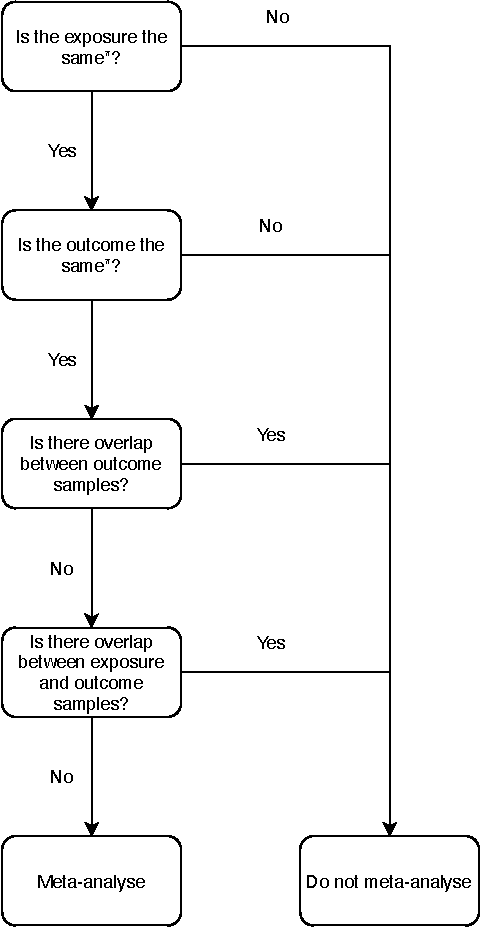
\includegraphics[width=0.6\linewidth]{data/SR/figures/meta_analysis_flowchart} 

}

\caption[Inclusion criteria for meta-analysis: flowchart]{\textbf{Inclusion criteria for meta-analysis: flowchart}. Mendelian randomization (MR) analyses were included in meta-analyses if they met the conditions set out in the flowchart and in Section \ref{SR-methods-meta-analysis} in regards to sample overlap. * = MR analyses had to use the same exposure and the same outcome to be compatible, e.g.~for the exposure, body mass index (BMI) could not be meta-analysed with any other exposure that was not BMI. This also applies to outcomes, e.g., the outcome oestrogen negative (ER-) breast cancer could not be meta-analysed with breast cancer, it could only be meta-analysed with ER- breast cancer.}\label{fig:SR-figure-meta-analysis-flowchart}
\end{figure}
\hypertarget{narrative-synthesis}{%
\subsection{Narrative synthesis}\label{narrative-synthesis}}

In order to gain a global picture of reported causal effects, a narrative synthesis was performed. All articles that were not included in the meta-analyses, and are therefore likely to be non-independent, were included in the narrative synthesis. MR analyses that were included in the meta-analyses were not included in the narrative synthesis. The outcome categories were used to guide the synthesis. The narrative synthesis summarised the reported directions of effect estimates across outcome categories, including a summary of the evidence for selected exposures and outcomes. Given that studies may not report p-values, these were not the focus here. The synthesis is presented in alphabetical order of the outcome categories.

\par

Given the non-independence of studies included in the meta-analysis, and the focus on summarising directions of effect estimates, the synthesis should be interpreted as an overview and not as definitive evidence for a causal effect. For a complete picture, or to look at specific exposure-outcome pairs, data are available on \href{https://github.com/mattlee821/000_thesis/blob/master/index/data/SR/analysis/data_extraction.xlsx}{GitHub}. When presenting results, ``increase'' and ``positive'' refer to, for example, a higher BMI or an increase in the risk of type-2 diabetes; ``decrease'' and ``negative'' refer to, for example, a lower BMI or a decreased risk of type-2 diabetes.

\par

\hypertarget{SR-results}{%
\section{Results}\label{SR-results}}

\hypertarget{literature-search}{%
\subsection{Literature search}\label{literature-search}}

In total, 8,376 articles were returned from the combined search of EMBASE (N = 3,772), MEDLINE (N = 3,638), and bioRxiv (N = 966). After combining the articles from EMBASE and MEDLINE, de-duplication resulted in the removal of 1,500 articles (N = 5,910). De-duplication of bioRxiv search results removed 293 articles (N = 673). Published bioRxiv articles were dealt with at the data extraction stage. The 5,910 articles from EMBASE and MEDLINE were combined with the 673 articles from bioRxiv and titles and abstracts were screened. A total of 277 articles were retained after title and abstract screening (\texttt{xml} file that can be imported into a reference manager is available on \href{https://github.com/mattlee821/000_thesis/tree/master/index/data/SR/data/full_text_screening_277.xml}{GitHub}).

\par

Of the 277 articles included in the full text screening, a total of 104 articles were removed for the following reasons (with number of articles removed indicated in brackets): a conference abstract with no response within 6 months from the author or there was no data available from the authors (25), conference abstracts with the full paper included in the search (23), duplicates not excluded by the de-duplication process (23), not using a measure of adiposity as the exposure (15), a commentary (8), erratum (3, the corrected papers were identified in the search), not MR (i.e., regression of single nucleotide polymorphism (SNP) on trait; 4), a conference proceeding (1), not available in English (1), and preprint paper in which the published paper did not include an MR of an adiposity measure (1). After full text screening, 173 articles were included in the analysis (PDFs available on \href{https://github.com/mattlee821/000_thesis/tree/master/index/data/SR/search/003_included_articles}{GitHub}).

\par

\newpage
\thispagestyle{empty}




\begin{figure}
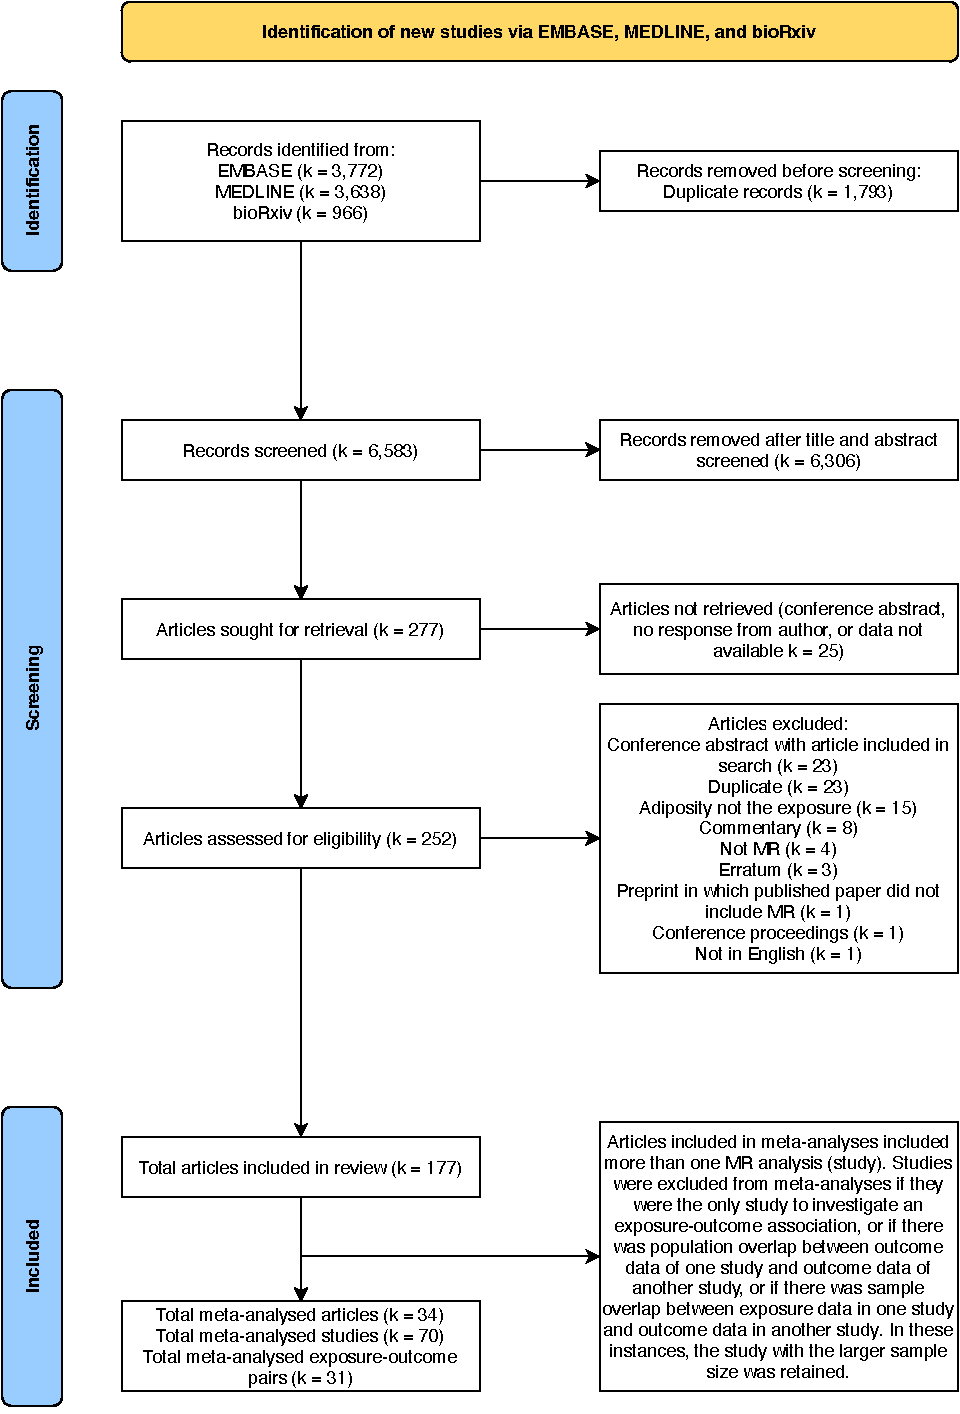
\includegraphics[width=0.9\linewidth]{data/SR/figures/PRISMA_flowchart} \caption[PRISMA flowchart]{\textbf{PRISMA flowchart}. \(k\) gives the number of articles at each stage. MR = Mendelian randomization}\label{fig:SR-prisma}
\end{figure}
\hypertarget{data-extraction-1}{%
\subsection{Data extraction}\label{data-extraction-1}}

Articles from bioRxiv included in data extraction were replaced with their published version if available. Of the 23 included bioRxiv articles, 18 were published once data extraction began and were included instead of the bioRxiv article. One bioRxiv article was excluded as the published version did not include the MR analysis. The remaining 4 bioRxiv articles were included. The majority of articles were published in the past 5 years (Figure \ref{fig:SR-figure-published-year}) and one-sample MR was the predominant analysis performed across the 173 studies (Figure \ref{fig:SR-figure-mr-design}).

\par




\begin{figure}

{\centering \includegraphics[width=1\linewidth]{thesis_files/figure-latex/SR-figure-published-year-1} 

}

\caption[Distribution of publication year per article and average exposure and outcome sample sizes across included studies up to February 2019]{\textbf{Distribution of publication year and average exposure and outcome sample sizes across included studies up to February 2019}. The number of articles included per year is given on the left Y axis; the right Y axis gives the average sample size for exposure (grey) and outcome (red) for each year. Outcome cases and controls were summed within analyses for binary outcomes.}\label{fig:SR-figure-published-year}
\end{figure}



\begin{figure}

{\centering \includegraphics[width=1\linewidth]{thesis_files/figure-latex/SR-figure-mr-design-1} 

}

\caption[Distribution of study design across 173 included articles]{\textbf{Distribution of study design across 173 included articles}. The majority of the 173 included articles reported more than one Mendelian randomization (MR) analysis. Where a study performed a bi-directional MR analysis and adiposity was the secondary analysis (i.e., to check for reverse causation), this was recorded as a bi-directional MR analysis. One-sample and two-sample MR meta-analysis indicates that the meta-analysis included MR analyses that were both one- and two-sample designs. Generalized summary data-based MR allows for, and models, correlated SNPs within the instrument. Factorial MR is analogous to a factorial randomized controlled trial, whereby individuals are grouped using genetic scores (generally in a 2 x 2 approach). An MR-PheWAS is the investigation of a single trait on many, potentially hundreds, of outcomes. Direct G-O refers to an MR analysis which used instruments from a single locus, e.g., the FTO locus.}\label{fig:SR-figure-mr-design}
\end{figure}
A total of 2,214 MR analyses were performed across the 173 studies (i.e., many studies conducted multiple MR analyses). This included 31 exposures and 659 outcomes. The majority of the 2214 MR analyses used BMI as the exposure (Table \ref{tab:SR-table-exposure-percentages}). After formatting the outcome data into three columns of (column 1) general outcome (e.g., breast cancer), (column 2), analysis specific outcome (eg., ER-), and outcome category (e.g., cancer), a total of 311 general outcomes were available and grouped into 16 outcome categories. Of the 311 outcomes, smoking was used in the most MR analyses followed by asthma and DNA methylation (Table \ref{tab:SR-table-outcome-percentages-10}). The largest proportion of outcomes were grouped into the metabolic and cancer categories (Table \ref{tab:SR-table-outcome-group-percentages}). The ``other'' category included 118 methylation outcomes, 68 mortality outcomes, and a handful of the following outcomes: age related macular degeneration, cataract, disease count, hernia, sleep, and physical activity. Categories, as discussed in the methods, were assigned based on prior biological knowledge.

\par
\begin{ThreePartTable}
\begin{TableNotes}[para]
\item BMI = body mass index; WHR = waist hip ratio; WHRadjBMI = WHR adjusted for BMI; WC = waist circumference; WCadjBMI = WC adjusted for BMI; HC = hip circumference; HCadjBMI = HC adjusted for BMI; BF = body fat percentage.
\end{TableNotes}
\begin{longtable}[t]{lrr}
\caption{\label{tab:SR-table-exposure-percentages}Number and frequency of exposures used across all 2214 MR analyses}\\
\toprule
Exposure & N & \%\\
\midrule
\endfirsthead
\caption[]{\label{tab:SR-table-exposure-percentages}Number and frequency of exposures used across all 2214 MR analyses \textit{(continued)}}\\
\toprule
Exposure & N & \%\\
\midrule
\endhead

\endfoot
\bottomrule
\insertTableNotes
\endlastfoot
\cellcolor{gray!6}{BMI} & \cellcolor{gray!6}{1509} & \cellcolor{gray!6}{68.16}\\
WHRadjBMI & 156 & 7.05\\
\cellcolor{gray!6}{WHR} & \cellcolor{gray!6}{112} & \cellcolor{gray!6}{5.06}\\
birth weight & 102 & 4.61\\
\cellcolor{gray!6}{WC} & \cellcolor{gray!6}{50} & \cellcolor{gray!6}{2.26}\\
\addlinespace
BF & 45 & 2.03\\
\cellcolor{gray!6}{fat mass} & \cellcolor{gray!6}{37} & \cellcolor{gray!6}{1.67}\\
BMI increasing and WHR decreasing & 20 & 0.90\\
\cellcolor{gray!6}{BMI increasing and WHR increasing} & \cellcolor{gray!6}{20} & \cellcolor{gray!6}{0.90}\\
obesity & 15 & 0.68\\
\addlinespace
\cellcolor{gray!6}{WCadjBMI} & \cellcolor{gray!6}{14} & \cellcolor{gray!6}{0.63}\\
fat percentage & 10 & 0.45\\
\cellcolor{gray!6}{HC} & \cellcolor{gray!6}{10} & \cellcolor{gray!6}{0.45}\\
hepatic fat & 10 & 0.45\\
\cellcolor{gray!6}{non-fat mass} & \cellcolor{gray!6}{10} & \cellcolor{gray!6}{0.45}\\
\addlinespace
sum of skinfolds & 10 & 0.45\\
\cellcolor{gray!6}{total body fat} & \cellcolor{gray!6}{10} & \cellcolor{gray!6}{0.45}\\
fat mass index & 9 & 0.41\\
\cellcolor{gray!6}{fat-free mass} & \cellcolor{gray!6}{9} & \cellcolor{gray!6}{0.41}\\
HCadjBMI & 9 & 0.41\\
\addlinespace
\cellcolor{gray!6}{favourable adiposity} & \cellcolor{gray!6}{7} & \cellcolor{gray!6}{0.32}\\
overweight & 7 & 0.32\\
\cellcolor{gray!6}{fat free mass} & \cellcolor{gray!6}{6} & \cellcolor{gray!6}{0.27}\\
lean mass & 6 & 0.27\\
\cellcolor{gray!6}{body fat mass} & \cellcolor{gray!6}{5} & \cellcolor{gray!6}{0.23}\\
\addlinespace
central obesity & 4 & 0.18\\
\cellcolor{gray!6}{adiponectin} & \cellcolor{gray!6}{3} & \cellcolor{gray!6}{0.14}\\
Obesity class 1 & 3 & 0.14\\
\cellcolor{gray!6}{weight} & \cellcolor{gray!6}{3} & \cellcolor{gray!6}{0.14}\\
body non-fat mass & 2 & 0.09\\
\addlinespace
\cellcolor{gray!6}{body fat} & \cellcolor{gray!6}{1} & \cellcolor{gray!6}{0.05}\\*
\end{longtable}
\end{ThreePartTable}
\begin{table}[H]

\caption{\label{tab:SR-table-outcome-percentages-10}Number and frequency of the 10 most used outcomes across all 2214 MR analyses}
\centering
\begin{tabular}[t]{lrr}
\toprule
Outcome & N & \%\\
\midrule
\cellcolor{gray!6}{smoking} & \cellcolor{gray!6}{175} & \cellcolor{gray!6}{7.90}\\
asthma & 122 & 5.51\\
\cellcolor{gray!6}{methylation (cpg)} & \cellcolor{gray!6}{118} & \cellcolor{gray!6}{5.33}\\
coronary artery disease & 87 & 3.93\\
\cellcolor{gray!6}{breast cancer} & \cellcolor{gray!6}{80} & \cellcolor{gray!6}{3.61}\\
\addlinespace
mortality & 68 & 3.07\\
\cellcolor{gray!6}{depression} & \cellcolor{gray!6}{58} & \cellcolor{gray!6}{2.62}\\
lung cancer & 52 & 2.35\\
\cellcolor{gray!6}{stroke} & \cellcolor{gray!6}{49} & \cellcolor{gray!6}{2.21}\\
osteoarthritis & 47 & 2.12\\
\bottomrule
\end{tabular}
\end{table}
\begin{table}[H]

\caption{\label{tab:SR-table-outcome-group-percentages}Number and frequency of outcomes within each outcome category across all 2214 MR analyses}
\centering
\begin{tabular}[t]{lrr}
\toprule
Group & N & \%\\
\midrule
\cellcolor{gray!6}{metabolic} & \cellcolor{gray!6}{404} & \cellcolor{gray!6}{18.25}\\
cancer & 352 & 15.90\\
\cellcolor{gray!6}{respiratory} & \cellcolor{gray!6}{318} & \cellcolor{gray!6}{14.36}\\
cardiovascular & 285 & 12.87\\
\cellcolor{gray!6}{other} & \cellcolor{gray!6}{235} & \cellcolor{gray!6}{10.61}\\
\addlinespace
mental health & 127 & 5.74\\
\cellcolor{gray!6}{skeletal} & \cellcolor{gray!6}{95} & \cellcolor{gray!6}{4.29}\\
anthropometric & 85 & 3.84\\
\cellcolor{gray!6}{brain} & \cellcolor{gray!6}{73} & \cellcolor{gray!6}{3.30}\\
hepatic & 71 & 3.21\\
\addlinespace
\cellcolor{gray!6}{social} & \cellcolor{gray!6}{71} & \cellcolor{gray!6}{3.21}\\
renal & 34 & 1.54\\
\cellcolor{gray!6}{reproductive} & \cellcolor{gray!6}{19} & \cellcolor{gray!6}{0.86}\\
gastrointestinal & 17 & 0.77\\
\cellcolor{gray!6}{skin} & \cellcolor{gray!6}{16} & \cellcolor{gray!6}{0.72}\\
\addlinespace
immune & 12 & 0.54\\
\bottomrule
\end{tabular}
\end{table}
\vspace*{-\baselineskip}

\noindent Outcome groups were assigned based on prior biological knowledge and aimed to collapse the large number of outcomes. This could be achieved differently for some outcomes, for example smoking could go in a `respiratory' group or a `behavioural' group. Where there were few outcomes to make a group, they were grouped into an `other' group. This will include outcomes such as mortality, disease counts, epigenetic markers, etc.

\par

\hypertarget{quality-assessment-1}{%
\subsection{Quality assessment}\label{quality-assessment-1}}

Studies that contributed to the meta-analyses were assessed for quality using a modified version of the assessment criteria devised by Mamluk et al.~(2020)\textsuperscript{\protect\hyperlink{ref-Mamluk2020}{429}}. Studies were assessed on a 3-point scale across 12 questions, with values ranging from 12-36. Analyses with lower scores (12-19) were considered to be of higher quality, with high scoring (28-36) studies considered lower quality. Scores in-between were of medium quality. The average assessment score was 24 (Figure \ref{fig:SR-figure-rob-distribution}). Individual studies were assessed as opposed to the article, as most articles conducted multiple studies. Only the study of the effect of BMI on hemorrhagic stroke by Dale et al (2017)\textsuperscript{\protect\hyperlink{ref-Dale2017}{451}} was ranked as high quality. The majority of studies (24) were assigned a medium quality score. All of the six low scoring studies showed consistent directions of effect with the other studies with which they were meta-analysed. Quality scores are presented alongside the meta-analysis results (Figures \ref{fig:SR-figure-forestplot-meta-analysis-binary} and \ref{fig:SR-figure-forestplot-meta-analysis-continuous}).

\par




\begin{figure}

{\centering \includegraphics{thesis_files/figure-latex/SR-figure-rob-distribution-1} 

}

\caption[Quality assessment: distribution of quality assessment scores for studies included in the meta-analyses]{\textbf{Quality assessment: distribution of quality assessment scores for studies included in the meta-analyses}. ``High'' indicates a study scored highly; ``low'' indicates a study scored poorly. QA = quality assessment score.}\label{fig:SR-figure-rob-distribution}
\end{figure}
\hypertarget{meta-analysis}{%
\subsection{Meta-analysis}\label{meta-analysis}}

In total, 31 meta-analyses were conducted using data from 34 articles, and 70 studies. A majority of studies were excluded due to a lack of meta-analysable data (i.e., only one MR analysis looked at a given exposure-outcome pair). Additional reasons for exclusion were: population overlap, incompatible units, and incompatible MR models. A majority of the 34 studies contributed to just one meta-analysis. A number of studies undertook multiple MR analyses which were included in multiple meta-analyses: four studies contributed to two meta-analyses, three studies to three meta-analyses, two studies to four meta-analyses, two studies to seven meta-analyses, and one study to eight meta-analyses (Table \ref{tab:SR-table-studies-N}).

\par
\begin{longtable}[]{@{}lr@{}}
\caption{\label{tab:SR-table-studies-N}Number of times an article was used in meta-analyses}\tabularnewline
\toprule
Article & N \\
\midrule
\endfirsthead
\toprule
Article & N \\
\midrule
\endhead
Gao et al.~2016\textsuperscript{\protect\hyperlink{ref-Gao2016}{452}} & 8 \\
Censin et al.~2019\textsuperscript{\protect\hyperlink{ref-Censin2019}{453}} & 7 \\
Fall et al.~2013\textsuperscript{\protect\hyperlink{ref-Fall2013}{412}} & 7 \\
Gharahkhani et al.~2019\textsuperscript{\protect\hyperlink{ref-Gharahkhani2019}{454}} & 4 \\
Holmes et al.~2014\textsuperscript{\protect\hyperlink{ref-Holmes2014}{413}} & 4 \\
Jarvis et al.~2016\textsuperscript{\protect\hyperlink{ref-Jarvis2016}{455}} & 3 \\
Wang et al.~2018\textsuperscript{\protect\hyperlink{ref-Wang2018}{456}} & 3 \\
Xu et al.~2017\textsuperscript{\protect\hyperlink{ref-Xu2017}{379}} & 3 \\
Dale et al.~2017\textsuperscript{\protect\hyperlink{ref-Dale2017}{451}} & 2 \\
Kar et al.~2018\textsuperscript{\protect\hyperlink{ref-Kar2019}{457}} & 2 \\
Shu et al.~2018\textsuperscript{\protect\hyperlink{ref-Shu2019}{458}} & 2 \\
Wurtz et al.~2014\textsuperscript{\protect\hyperlink{ref-Wurtz2014}{286}} & 2 \\
Ostegaard et al, 2015\textsuperscript{\protect\hyperlink{ref-Ostergaard2015}{459}} & 1 \\
Brower et al.~2018\textsuperscript{\protect\hyperlink{ref-Brower2019}{460}} & 1 \\
Day et al.~2018\textsuperscript{\protect\hyperlink{ref-Day2018}{461}} & 1 \\
Kivimaki et al.~2008\textsuperscript{\protect\hyperlink{ref-Kivimaki2008}{462}} & 1 \\
Klarin et al.~2017\textsuperscript{\protect\hyperlink{ref-Klarin2017}{463}} & 1 \\
Larsson et al.~2017\textsuperscript{\protect\hyperlink{ref-Larsson2017}{464}} & 1 \\
Larsson et al.~2018\textsuperscript{\protect\hyperlink{ref-Larsson2018}{465}} & 1 \\
Lindstrom et al.~2017\textsuperscript{\protect\hyperlink{ref-Lindstrom2017}{466}} & 1 \\
Lv et al.~2018\textsuperscript{\protect\hyperlink{ref-Lv2018}{467}} & 1 \\
Lyall et al.~2016\textsuperscript{\protect\hyperlink{ref-Lyall2017}{468}} & 1 \\
Nordestgaard et al.~2017\textsuperscript{\protect\hyperlink{ref-Nordestgaard2017}{469}} & 1 \\
Painter et al.~2016\textsuperscript{\protect\hyperlink{ref-Painter2016}{470}} & 1 \\
Palmer et al.~2011\textsuperscript{\protect\hyperlink{ref-Palmer2011}{471}} & 1 \\
Richardson et al.~2019\textsuperscript{\protect\hyperlink{ref-Richardson2019a}{472}} & 1 \\
Shapland et al.~2019\textsuperscript{\protect\hyperlink{ref-Shapland2019}{473}} & 1 \\
Skaaby et al.~2018\textsuperscript{\protect\hyperlink{ref-Skaaby2018}{474}} & 1 \\
Speed et al.~2019\textsuperscript{\protect\hyperlink{ref-Speed2019}{475}} & 1 \\
Tyrrell et al.~2019\textsuperscript{\protect\hyperlink{ref-Tyrrell2019}{476}} & 1 \\
van den Broek et al.~2018\textsuperscript{\protect\hyperlink{ref-VandenBroek2018}{477}} & 1 \\
Wade et al.~2018\textsuperscript{\protect\hyperlink{ref-Wade2018}{478}} & 1 \\
Wang et al.~2018\textsuperscript{\protect\hyperlink{ref-Wang2018a}{479}} & 1 \\
Yarmolinsky et al.~2019\textsuperscript{\protect\hyperlink{ref-Yarmolinsky2019}{480}} & 1 \\
\bottomrule
\end{longtable}
For all binary outcomes, results are given per SD unit increase, such that an odds ratio (OR) is the change in the outcome per SD unit increase in the exposure. Studies which used risk ratios and hazard ratios were excluded from the meta-analysis following the rules set out in Figure \ref{fig:SR-figure-meta-analysis-flowchart}, e.g., sample overlap. For continuous outcomes, results are given as the mean difference (MD) and reflect an average unit change in the outcome per SD unit increase in the exposure. The term ``effect estimate'' is used throughout.

\par

In the meta-analyses, there were 22 binary outcomes and 9 continuous outcomes. Overall, the strongest and most consistent evidence across the meta-analysis suggested a causal effect of BMI on endometrial, colorectal, ovarian, and lung cancers, as well as ischemic stroke, venous thromboembolism, type 2 diabetes, SBP and fasting glucose; of WHR on colorectal cancer and CAD; and of WHRadjBMI on CAD. For the 22 binary outcomes, 2 tests (birthweight on ER- breast cancer and coronary artery disease (CAD)) had negative effect estimates. Both tests had CIs which spanned the null. The remaining 20 tests had positive effect estimates, 13 of which had CIs that did not span the null (Figure \ref{fig:SR-figure-forestplot-meta-analysis-binary}). The majority of MR analyses included in these meta-analyses had a medium quality assessment score. The MR analysis by Dale et al., (2017)\textsuperscript{\protect\hyperlink{ref-Dale2017}{451}} of BMI on haemorrhagic stroke was the only analysis to score highly. The four studies which had a low quality assessment score did not have weights that were drastically different compared to the other MR analyses in those meta-analyses; all but one had tight CIs which did not cross the null.

\par

For the 9 continuous outcomes, 3 tests (BMI on high density lipoprotein (HDL; analysed with SD and mmol/L units) and low density lipoprotein (LDL; mmol/L)), had negative effect estimates with CIs which spanned the null. The remaining 6 tests had positive effect estimates, 2 (BMI on systolic blood pressure (SBP; mmHg) and fasting glucose (mmol/L)) of which had CIs that did not span the null (Figure \ref{fig:SR-figure-forestplot-meta-analysis-continuous}). Two meta-analyses included MR studies which were ranked low for quality assessment; the study by Shapland et al., (2018)\textsuperscript{\protect\hyperlink{ref-Shapland2019}{473}} had comparable weight to the other two studies investigating BMI on SBP. The study by Wang et al., (2018)\textsuperscript{\protect\hyperlink{ref-Wang2018a}{479}} investigating Homoeostatic Model Assessment for Insulin Resistance (HOMA IR) had a much larger weight than the study by Kivimaki et al., (2008)\textsuperscript{\protect\hyperlink{ref-Kivimaki2008}{462}}, a result of a larger population. The remaining studies had a medium quality assessment score, none of which showed estimates that deviated strongly from the effects of the other MR analyses in those meta-analyses.

\par

\newpage
\thispagestyle{empty}
\vspace*{-3cm}




\begin{figure}

{\centering 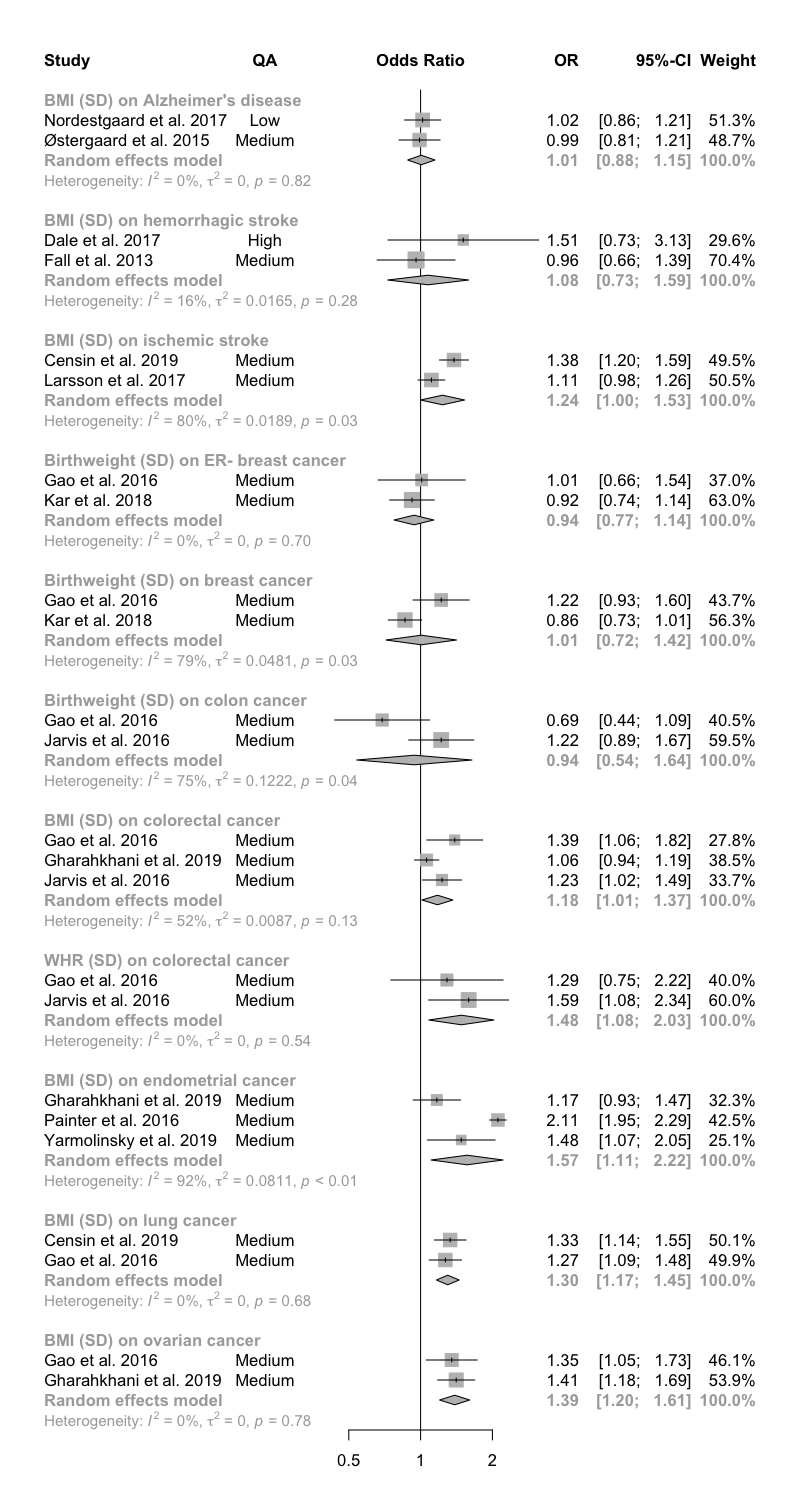
\includegraphics[width=0.8\linewidth]{../../005_systematic_review/figures/meta_analysis_results_figures/binary_outcomes1} 

}

\caption[Meta-analysis: effect estimates and 95\% confidence intervals for binary outcomes]{\textbf{Meta-analysis: effect estimates and 95\% confidence intervals for binary outcomes}. Forest plot shows effect estimates and 95\% confidence intervals (CIs) from a meta-analysis of 22 different exposure-outcome pairs. MR analyses included based on criteria in Figure \ref{fig:SR-figure-meta-analysis-flowchart}. QA = quality assessment score; OR = odds ratio; CI = confidence interval. Available on \href{https://github.com/mattlee821/000_thesis/blob/master/index/data/SR/figures/meta_analysis_results_figures/binary_outcomes1.pdf}{GitHub}. Forest plots of individual meta-analyses are also available on \href{https://github.com/mattlee821/000_thesis/tree/master/index/data/SR/figures/meta_analysis_results_figures}{GitHub}.}\label{fig:SR-figure-forestplot-meta-analysis-binary}
\end{figure}
\newpage
\thispagestyle{empty}
\vspace*{-3cm}




\begin{figure}

{\centering 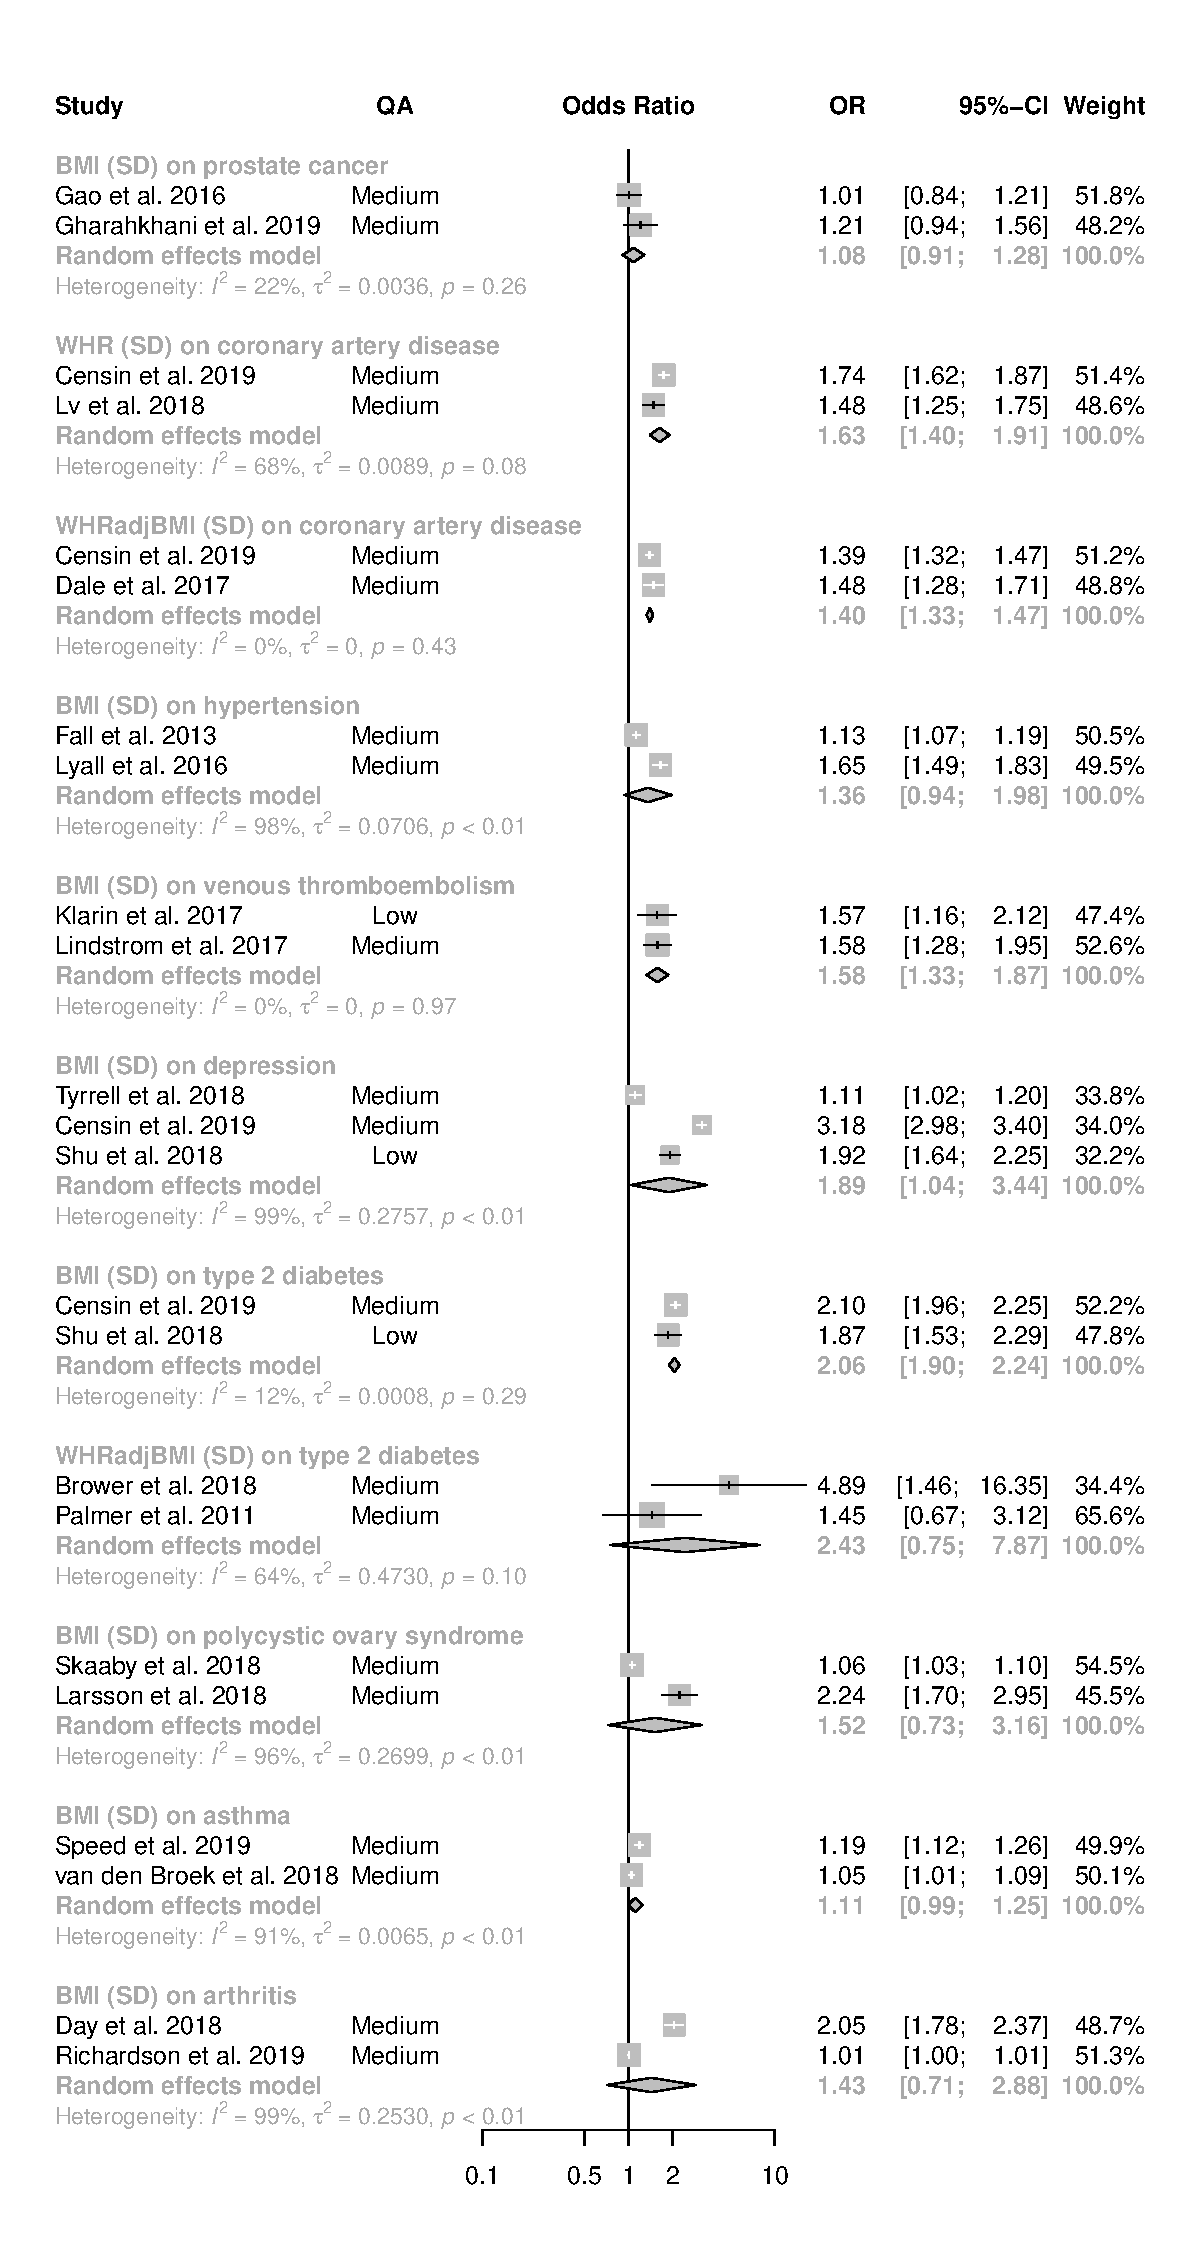
\includegraphics[width=0.8\linewidth]{../../005_systematic_review/figures/meta_analysis_results_figures/binary_outcomes2} 

}

\caption[Meta-analysis: effect estimates and 95\% confidence intervals for binary outcomes]{\textbf{Meta-analysis: effect estimates and 95\% confidence intervals for binary outcomes continued}. Forest plot shows effect estimates and 95\% confidence intervals (CIs) from a meta-analysis of 22 different exposure-outcome pairs. MR analyses included based on criteria in Figure \ref{fig:SR-figure-meta-analysis-flowchart}. QA = quality assessment score; OR = odds ratio; CI = confidence interval. Available on \href{https://github.com/mattlee821/000_thesis/blob/master/index/data/SR/figures/meta_analysis_results_figures/binary_outcomes2.pdf}{GitHub}. Forest plots of individual meta-analyses are also available on \href{https://github.com/mattlee821/000_thesis/tree/master/index/data/SR/figures/meta_analysis_results_figures}{GitHub}.}\label{fig:SR-figure-forestplot-meta-analysis-binary2}
\end{figure}
\newpage
\thispagestyle{empty}




\begin{figure}

{\centering 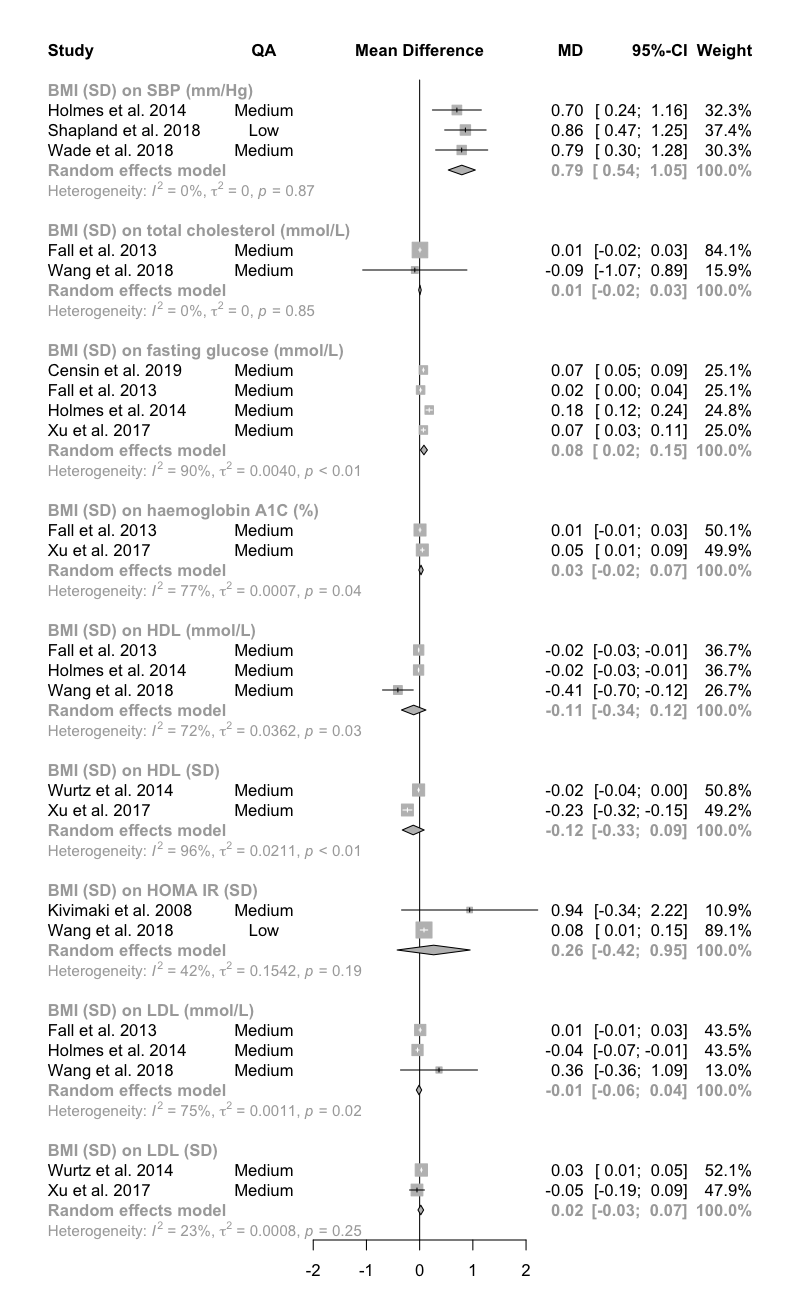
\includegraphics[width=0.8\linewidth]{../../005_systematic_review/figures/meta_analysis_results_figures/continuous_outcomes} 

}

\caption[Meta-analysis: effect estimates and 95\% confidence intervals for continuous outcomes]{\textbf{Meta-analysis: effect estimates and 95\% confidence intervals for continuous outcomes}. Forest plot shows effect estimates and 95\% confidence intervals (CIs) from a meta-analysis of 9 different exposure-outcome pairs. MR analyses included based on criteria in Figure \ref{fig:SR-figure-meta-analysis-flowchart}. QA = quality assessment score; MD = mean difference; CI = confidence interval. Available on \href{https://github.com/mattlee821/000_thesis/blob/master/index/data/SR/figures/meta_analysis_results_figures/continuous_outcomes.pdf}{GitHub}. Forest plots of individual meta-analyses are also available on \href{https://github.com/mattlee821/000_thesis/tree/master/index/data/SR/figures/meta_analysis_results_figures}{GitHub}.}\label{fig:SR-figure-forestplot-meta-analysis-continuous}
\end{figure}
Three outcomes were investigated using more than one exposure, CAD with waist hip ratio (WHR) and WHR adjusted for BMI (WHRadjBMI), colorectal cancer with BMI and WHR, and type 2 diabetes with BMI and WHRadjBMI. There was strong evidence for an effect of WHR (OR per SD unit increase = 1.63; 95\% confidence interval (CI) = 1.4 -- 1.91) and WHRadjBMI (OR per SD unit increase = 1.4; 95\% CI = 1.33 -- 1.47) on CAD. When looking at colorectal cancer, WHR (OR per SD unit increase = 1.48; 95\% CI = 1.08 -- 2.03) and BMI (OR per SD unit increase = 1.18; 95\% CI = 1.01 -- 1.37) showed similar effects with overlapping CIs. For type 2 diabetes, BMI (OR per SD unit increase = 2.48; 95\% CI = 1.52 -- 4.07) and WHRadjBMI (OR per SD unit increase = 2.06; 95\% CI = 1.9 -- 2.24) both showed strong estimates with overlapping CIs.

\par

All remaining tests were conducted with BMI (in SD units) as the exposure. Except for the negative effect on breast cancer, BMI was found to be associated with an increase in all cancers tested (colorectal, endometrial, lung, ovarian, and prostate), CIs crossed the null only for prostate cancer (OR = 1.08; 95\% CI = 0.91 -- 1.28). The strongest evidence for an effect was found for venous thromboembolism (OR = 1.58; 95\% CI = 1.33 -- 1.87) and type 2 diabetes (OR = 2.48; 95\% CI = 1.52 -- 4.07) - asthma also showed strong evidence but with a smaller effect size (OR = 1.06; 95\% CI = 1.03 -- 1.1). There was weak evidence for an effect of BMI on ischemic and haemorrhagic stroke, hypertension, arthritis, and Alzheimer's disease, with effect estimates close to the null and CIs spanning the null.

\par

The weights for each study included in the individual meta-analyses were broadly even (e.g., in a meta-analysis of three studies, each study had a weighting of roughly 33\%). The exceptions, where one study had a much larger or much smaller weight than the other(s) was for: BMI and asthma, BMI and polycystic ovary syndrome (PCOS), BMI and haemorrhagic stroke, BMI and total cholesterol, BMI and HOMA IR, and BMI and LDL. There was evidence of heterogeneity within the included studies, 8 of 22 binary outcomes and 5 of 9 continuous outcomes had heterogeneity statistics with p-values \textless{} 0.05, e.g., BMI on endometrial cancer \emph{I\textsuperscript{2}} = 92\% (p-value \textless{} 0.01; Table \ref{tab:appendix-SR-table-meta-analyses-results}). However, given no meta-analysis met the requirements for heterogeneity statistics (\(\geq\) 5 studies; See \href{https://training.cochrane.org/handbook/current/chapter-10\#section-10-10-2}{Cochrane Handbook})\textsuperscript{\protect\hyperlink{ref-VonHippel2015}{481}}, these results should be interpreted with caution. Heterogeneity statistics and weights are presented in Figures \ref{fig:SR-figure-forestplot-meta-analysis-binary} and \ref{fig:SR-figure-forestplot-meta-analysis-continuous}, as well as Appendix Table \ref{tab:appendix-SR-table-meta-analyses-results}.

\par

\hypertarget{narrative-synthesis-1}{%
\subsection{Narrative synthesis}\label{narrative-synthesis-1}}

A total of 2144 studies were not included in the meta-analyses. Though many of these could not be included because they did not meet certain requirements for inclusion (e.g., overlapping populations), they still provide information on the potential effects of adiposity. Using the 16 categories used to group outcomes, these effects are summarised here, in alphabetical order with the ``other'' category at the end. Where there are a large number of studies, a summary of the directions of effect are given. Given that studies use a variety of transformations, units, and models, comparison of the magnitude of effect is not appropriate. Instead, the focus here is on directions of effect estimates and whether evidence is consistent across studies. Evidence for selected exposure-outcome pairs is also summarised. For a complete picture, or to look at specific exposure-outcome pairs, data are available on \href{https://github.com/mattlee821/000_thesis/blob/master/index/data/SR/analysis/data_extraction.xlsx}{GitHub}.

\par

\hypertarget{anthropometric}{%
\subsubsection{Anthropometric}\label{anthropometric}}

A total of 85 studies were reported across 9 articles for anthropometric outcomes. These studies were generally investigating the effect of maternal adiposity on offspring anthropometric traits. This included analyses of birthweight, BMI, hip circumference adjusted for BMI (HCadjBMI), waist circumference adjusted for BMI (WCadjBMI), and WHRadjBMI on similar anthropometric traits such as adipose tissue volume, birth length, body fat, head circumference, leg fat, and trunk fat. The majority of effect estimates were positive (N = 60; negative = 24). A single MR analysis (BMI on offspring BMI) had an effect estimate of 0. A number of other analyses focussed on offspring traits as the outcome with both positive and negative effect estimates. The study by Winkler et al.~(2018)\textsuperscript{\protect\hyperlink{ref-Winkler2018}{36}} used a unique instrumentation method, using a composite measure of BMI, WHR, and WHRadjBMI, for example BMI increasing and WHR increasing SNPs were used as a genetic instrument. Generally, the effect of adiposity on anthropmetric traits was to increase them, but this is likely a reciprocal relationship, i.e., increased BMI leads to increased WHR and increased WHR leads to increased BMI.

\par

\hypertarget{cancer-1}{%
\subsubsection{Cancer}\label{cancer-1}}

A total of 332 studies were reported across 39 articles for cancer-related outcomes. This included analyses of all cancers, cancer mortality, cancer types such as breast and prostate, and subtypes such as ER- and ER+ breast cancer. A majority of effect estimates were positive (N = 189; negative = 137), while six studies of breast, kidney, lung, and prostate cancer showed effect estimates approximately equal to 1. A majority of analyses with positive effect estimates had CIs which spanned the null. The same was true for negative effect estimates.

\par

Of the 31 cancer outcomes, three showed negative effect estimates -- cervical (with BMI and WHRadjBMI), clear cell (with BMI), and gastric (with BMI) cancers -- while 14 showed positive effect estimates. This included overall cancer mortality (with BMI) and cancer risk (with BMI). The remaining cancer types with positive effect estimates included Barrett's esophagus (with BMI), colon (with BMI), esophageal (with BMI), lymphoid (with BMI), meningioma (with BMI, WC, and BF), rectal (with BMI), renal (with BMI, WHR, and BF), skin (including melanoma; with BMI), and stomach and esophageal (with BMI). Low malignant potential tumors also showed a positive effect estimate with BMI. The remaining 13 cancer types had positive and negative effect estimates. This included any cancer, breast, colorectal, endometrial, glioma, kidney, lung, multiple myeloma, ovarian, pancreatic, prostate, testicular, and upper aerodigsetive cancers.

\par

Results suggest adiposity increases overall cancer risk and risk of mortality. However, this risk is modulated by cancer type and subtype. In the case of cancers with only negative effect estimates, these cancers were only analysed once, where as cancers like breast and lung, which where measured multiple times, showed both positive and negative effect estimates.

\par

\hypertarget{cardiovascular-1}{%
\subsubsection{Cardiovascular}\label{cardiovascular-1}}

A total of 274 studies were reported across 50 articles for cardiovascular-related outcomes. This included analyses of 11 continuous traits and 19 binary outcomes. Exposures included birth weight, BMI, body fat mass measures, HC, WC, WCadjBMI, weight, WHR, and WHRadjBMI.

\par

In total, 83 studies investigating the effect of adiposity with continuous traits were reported across 22 articles. The majority of these studies reported positive effect estimates (N = 69; negative = 14). Of the 11 traits, four had a single reported MR result (left ventricular mass, mean arterial pressure, pulse pressure, and pulse wave velocity) -- all had positive effect estimates except pulse wave velocity. Of the seven remaining traits, five had both positive and negative effect estimates. Effects on heart rate were negative with wide CIs, while effects on carotid-intima media thickness (IMT) were positive with some studies reporting effect estimates with CIs that did not overlap the null for BMI and WHRadjBMI.

\par

Of the five traits with positive and negative effect estimates, diastolic blood pressure (DBP) showed a negative effect estimate solely in relation to the effect of birthweight, and SBP showed weak evidence for a decreasing effect of BMI and birthweight. There was much stronger evidence for an increasing effect on SBP and DBP across BMI, WHR, and WHRadjBMI. The positive and negative effect estimates associated with heart beat were associated with CIs which spanned the null for both BMI and WHRadjBMI. For carotid IMT, evidence appeared stronger, with narrower CIs which did not spanned the null, for an increasing effect of BMI. Evidence for an effect of BMI and WHRadjBMi on left ventricular hypertrophy was weak and dependent upon the method used to assess hypertrophy.

\par

In total, 191 studies investigating the effect of adiposity with binary outcomes were reported across 35 articles. Nine of these studies were from a single article which only reported p-values for the effect of BMI on CAD. Of the remaining 182 studies, the majority reported positive effect estimates (N = 139; negative = 43). There was strong evidence across multiple studies for the effect of BMI on CAD and CVD and results also supported an effect of WHRadjBMI, WCadjBMI, and WHR. Though there was evidence for an effect of BMI on heart failure, there was weak evidence for a similar effect of WHRadjBMI on the same outcome. There was strong evidence for an effect of fat mass and fat free mass on increased risk of arrythmia, but only weak evidence for a similar effect from WHRadjBMI and birthweight. There was conflicting evidence for an effect of increased BMI on myocardial infarction (MI). When using BMI increasing and WHR decreasing instruments MI risk decreased while when using BMI and WHR increasing instruments, MI risk increased. There was also weak evidence of increased birthweight reducing MI risk. There was strong evidence across many different adiposity measures for an increased risk of deep vein thrombosis (DVT).

\par

Though there were some conflicting results, BMI and MI for example, and some analyses reported both positive and negeative effect estimates for the same exposure-outcome pairs, BMI and SBP for example, on balance reported results support an increasing effect of adiposity on cardiovascular traits. Evidence was strongest for the effect of adiposity on CAD, CVD, and DVT.

\par

\hypertarget{gastrointestinal}{%
\subsubsection{Gastrointestinal}\label{gastrointestinal}}

A total of 17 studies were reported across 5 articles for gastrointestinal-related outcomes. This included analyses of inflammatory bowel disorders, \emph{Helicobacter pylori} infection measures, gallstone disease, and peptic ulcers. All but one analysis of the effect of of BMI on irritable bowel syndrome had a positive direction of effect. There was evidence for an effect of birthweight on inflammatory bowel disease and some evidence for an effect of BMI on peptic ulcers, however weak evidence for an effect of WHRadjBMI on peptic ulcers. All other analyses showed weak evidence of effect. As no exposure-outcome pairs were analysed by more than one study, it is hard to draw conclusions from the available evidence, however effect estimates were mostly positive across studies.

\par

\hypertarget{hepatic}{%
\subsubsection{Hepatic}\label{hepatic}}

A total of 71 studies were reported across 6 articles for hepatic-related outcomes. In total, 11 outcomes were reported, of which the majority of analyses (N = 40) were for three liver markers: alanine transaminase (ALT), aspartate transaminase (AST), and gamma-glutamyl Transferase (GGT). All but two binary outcomes (the effect of low BMI and low alcohol consumption on liver disease) had positive directions of effect. 14 of the 40 liver markers had negative directions of effect. AST was reported once with strong evidence of a reducing effect of BMI. Analyses of ALT and GGT used multiple measures across multiple studies, for example adjusting for alcohol consumption. Results support an increasing effect of increased BMI on ALT and GGT, which persisted after adjustment for alcohol consumption. The remaining 8 outcomes were only investigated by a single article. Evidence was found for BMI and WHR on chronic liver disease and BMI, WHR, and WHRadjBMI on NAFLD. There was strong evidence for an increasing effect of adiposity on all hepatic traits.

\par

\hypertarget{inflammation-and-immunity-1}{%
\subsubsection{Inflammation and immunity}\label{inflammation-and-immunity-1}}

A total of 12 studies were reported across 5 artciles for immune-related outcomes. In total, 8 outcomes were reported. Seven studies reported negative directions of effect; five studies reported postivie directions of effect. There was weak evidence for an effect of adiposity on all outcomes, except for an increasing effect of BMI on dermatophytosis (though weak evidence for an effect of WHRadjBMI) and BMI on psoriasis.

\par

\hypertarget{mental-health}{%
\subsubsection{Mental health}\label{mental-health}}

A total of 124 studies were reported across 22 articles for mental health-related outcomes. A total of 66 studies reported positive directions of effect; 38 studies reported negative directions of effect; 4 studies reported effect estimates equal to 0; the remaining studies did not report an effect estimate. In total, 27 outcomes were reported, though 16 of these were reported only once - all showed weak evidence of an effect (e.g., attention deficit hyperactivity disorder, anorexia nervosa, being a worrier/nervous person, body dissatisfaction (evidence from weight and shape concern analyses showed a negative effect of BMI), and happiness). Of the remaining 11 outcomes, the majority of analyses focussed on depression. Across the 11 articles which looked at depression, there was strong evidence for an effect of adiposity increasing depression. When excluding non-neuronal SNPs (which will influence adiposity at a cellular as opposed to behavioural level), the effect of BMI was reduced and CIs crossed the null\textsuperscript{\protect\hyperlink{ref-Tyrrell2019}{476}}. This would suggest that the association with depression is not a result of behavioural changes associated with adiposity. Rather, the association is likely due to the physicality of adiposity and probably the stigmatization associated with that. There was weak evidence for an effect of BMI on anxiety. There was weak evidence for an effect of increased BMI on increased loneliness. Similarly, there was weak evidence for a decreasing effect of BMI, WHR, WC, and BF on subjective wellbeing. There was some evidence for a decreasing effect of BMI and WHR on stress/nervous feelings, however weak evidence was found for all other psychological distress traits. Binge eating and overeating increased as a result of increased BMI. On balance, there appears to be an association between adiposity and mental health traits, particularly body image-related traits. However, this association is likely not a direct result of adipose tissue, but is perhaps a result of sociological factors.

\par

\hypertarget{metabolic}{%
\subsubsection{Metabolic}\label{metabolic}}

A total of 380 studies were reported across 51 articles for metabolic-related outcomes. In total, 27 outcomes were reported. A total of 266 studies reported negative effect estimates; 89 studies reported positive effect estimates; the remianing studies did not report effect estimates. A majority of studies were of the effect of metabolites, many of which were reported once. Although the majority of metabolite effect estimates were positive, CIs for many spanned the null. There was, for example, weak evidence for an increasing effect of BMI on cholesterol, however strong evidence for an effect of WHRadjBMI. C-reactive protein (CRP) was investigated with BMI across 9 studies with all but two reporting strong evidence for an increasing effect of BMI on CRP levels. BMI was found to decrease levels of apolipoprotein A-I and increase apolipoprotein B levels; there was weak evidence for an increasing effect of BMI and WHRadjBMI on apolipoprotein A-IV. There was strong evidence for a decreasing effect of BMI, WHRadjBMI, and birthweight on HDL levels; there was weaker evidence for an overall effect of adiposity on LDL -- WHRadjBMI was strongly associated with a increase in LDL, while birthweight showed a decreasing effect on LDL. BMI showed weak evidence of both increasing and decreasing effects on LDL. There was also strong evidence for an increasing effect of BMI, WHR, and WHRadjBMi on triglycerides (TG).

\par

There was strong evidence for an effect of increased BMI, WHR, WHRadjBMI on fasting glucose; there was weaker evidence for an effect of childhood BMI and birthweight on fasting glucose. There was weak evidence for an effect of BMI (adult and childhood) on two hour glucose test (there was evidence for a decreasing effect of birth weight), and weak evidence for an increasing effect of BMI on non-fasting glucose. There was strong evidence for an effect of BMI on hyperuricaemia as well as uric acid. Weaker evidence was reported for an effect of BMI (adult and childhood) and WHRadjBMI on glomerular filtration rate, creatine, and creatinine. There was strong evidence for an increasing effect of BMI, WHR, and WHRadjBMI on fasting insulin. There was however weak evidence for an increasing effect of BMI on insulin secretion. Binary outcomes reported broadly increasing effects of adiposity. For example, there was strong evidence for an effect of increased BMI on increased diabetes (type-1, type-2, and all). Similarly strong evidence was reported when using birthweight, childhood BMI, WHR, WHRadjBMI, and WC. Strong evidence for an effect of BMI and WHRadjBMI on increased dyslipidemia and metabolic syndrome was reported, but there was weak evidence for an effect of BMI and WHRadjBMI on hyper- and hypo-thyroidism and iron deficiency. The effect of adiposity appears far reaching in regards to metabolic traits. This effect is generally to increase levels of traits that are themselves associated with poor health outcomes.

\par

\hypertarget{neurologicalbehavioural-1}{%
\subsubsection{Neurological/behavioural}\label{neurologicalbehavioural-1}}

A total of 67 studies were reported across 21 articles for brain-related outcomes. This included analyses of Alzheimer's disease, amyotrophic lateral sclerosis (ALS), dementia, multiple sclerosis (MS), Parkinson's disease, and stroke. Bipolar disorder, schizophrenia, cognitive ability, grey matter volume, and migraine were also present. Exposures included birth weight, BMI, WHR, and WHRadjBMI - BMI was used in the majority of analyses. The majority of effect estimates were positive (N = 45; negative = 17). Two analyses (BMI on stroke (ischemic small vessel) and dementia) had an OR of \(1\). Effect estimates appeared larger on the whole when in the positive direction, however in many cases across both the positive and negative estimates, CIs spanned the null. On balance, results suggest adiposity increases the risk of all types of stroke. However, for all other outcomes, there appears conflicting or weak evidence for an effect.

\par

\hypertarget{renal}{%
\subsubsection{Renal}\label{renal}}

A total of 34 studies were reported across 4 articles for renal-related outcomes. Only one study, the effect of WHRadjBMI on renal failure, reported a negative direction of effect. All other studies reported a positive direction of effect. A majority of analyses looked at renal failure (N = 20) which showed strong evidence for an increasing effect of BMI, WHR, and WHRadjBMI. These analyses were however from a single study\textsuperscript{\protect\hyperlink{ref-Censin2019}{453}}. A similar picture is present for BMI and renal disease which was investigated by a single study\textsuperscript{\protect\hyperlink{ref-Todd2015}{482}}, as well as macroalbuminuria and BMI\textsuperscript{\protect\hyperlink{ref-Todd2015}{482}}. There was weak evidence for an increasing effect of childhood BMI and birth weight on chronic kidney disease. As few articles looked at renal-related outcomes, it is difficult to draw conclusions given a lack of replication. However, the general trend is for an increasing effect of adiposity on the risk of renal-related traits and renal diseases.

\par

\hypertarget{reproductive-1}{%
\subsubsection{Reproductive}\label{reproductive-1}}

A total of 17 studies were reported across 5 articles primarily for menarche (age at and early onset). All studies reported positive directions of effect except for the two studies on age at menarche. The two studies reporting on age at menarche and BMI and childhood BMI found strong evidence that adiposity decreased age at menarche,\textsuperscript{\protect\hyperlink{ref-Millard2015}{483},\protect\hyperlink{ref-Mumby2011}{484}} which is associated with poor health outcomes in later life. The remaining 15 analyses on early menarche were reported by one study\textsuperscript{\protect\hyperlink{ref-Fan2018}{485}} and showed evidence that BMI, total body fat, fat free mass, sum of skinfolds, HC, and WHR all lead to an earlier menarche. One study reported evidence of an increasing effect of BMI on PCOS\textsuperscript{\protect\hyperlink{ref-Day2018}{461}}, while another reported weak evidence for an increasing effect of WHRadjBMI on uterine fibroids\textsuperscript{\protect\hyperlink{ref-Emdin2017}{486}}. There is clear evidence that adiposity increases the likelihood of early menarche. There is therefore compelling evidence that adiposity is detrimental in regards to all reproductive traits.

\par

\hypertarget{respiratory-1}{%
\subsubsection{Respiratory}\label{respiratory-1}}

A total of 316 studies were reported across 13 articles for respiratory-related outcomes. A majority of these analyses were for smoking outcomes (N = 175) such as age at initiation, status, number of cigarettes per day, as well as comparisons between smoking status (e.g., ever vs never). Of the non-smoking respiratory studies, 11 studies reported negative directions of effect, the remaining 123 reported positive directions of effect. Of the smoking respiratory studies, 81 reported negative directions of effect and 90 reported positive directions of effect. There was strong evidence for an effect of BMI, WHR, and WHRadjBMI on current smoking status. There was also evidence for a positive effect of BMI on lifetime smoking. There was weak evidence for an effect of BMI on former vs current and experimental vs never smoking. There was some evidence for an effect of BMI on ever vs never smoking, increasing the odds of being an ever smoker. There was similarly an increasing effect on ever being a smoker for BMI, WC, and BF -- this effect modulated when including/excluding neuronal/deprivation related SNPs. The majority of the remaining studies were for asthma and asthma subtypes. There was broadly weak evidence for an increasing effect of BMI on asthma. There was some evidence for an increasing effect of BMI on chronic obstructive pulmonary disorder as well as for an increasing effect of BMI on wheezing, and decreased lung volume measures (forced vital capacity and forced expiratory volume). Overall adiposity appears to increase the likelihood of being a smoker as well as having respiratory conditions such as asthma.

\par

\hypertarget{skeletal}{%
\subsubsection{Skeletal}\label{skeletal}}

A total of 93 studies were reported across 13 articles for skeletal-related outcomes. A total of 20 studies reported negative directions of effect; 70 reported positive directions of effect; 3 did not report an effect estimate. A majority of studies were for arthritic outcomes (arthritis and osteoarthritis), though evidence was conflicting. There was some evidence for an increasing effect of BMI on rheumatoid arthritis and gout, however weak evidence for an effect of WHRadjBMI. Strong evidence was reported for an increasing effect of BMI, WC, and HC on osteoarthritis (self report, hospital diagnosed: hip, knee), however weak evidence for an effect of WHR and birth weight. One study reported an effect of BMI on osteoporosis, where there was evidence of an increasing effect. There was strong evidence for an increasing effect of BMI and fat mass on bone mineral density (including site-specific bone mineral density), and some evidence for an increasing effect of trunk fat mass on bone mineral content. On balance, the effect of adiposity is detrimental to skeletal traits. This is especially true for arthritic traits, where body composition as opposed to deposition appears to be more important.

\par

\hypertarget{skin}{%
\subsubsection{Skin}\label{skin}}

A total of 16 studies were reported in 1 article\textsuperscript{\protect\hyperlink{ref-Budu-Aggrey2019}{487}}. Budu-Aggrey et al., (2019) investigated the effect of BMI on psoriasis using one- and two-sample MR analyses. To strengthen evidence for a causal effect, they meta-analysed one- and two-sample MR results and performed the reverse MR investigating the effect of psoriasis on BMI. All studies reported a positive direction of effect. There was strong evidence for an increasing effect of BMI on psoriasis and weak evidence for an effect of psoriasis on BMI.

\par

\hypertarget{social}{%
\subsubsection{Social}\label{social}}

A total of 71 studies were reported across 12 articles for social-related traits such as income, education, and employment. A total of 14 studies investigated the efefct of adiposity on income, 9 of these reported a negative direction of effect and 5 reported a positive direction of effect. Of the remaining 57 non-income related studies, 41 reported a negative direction of effect, 12 reported a positive direction of effect, and 4 reported an effect estimate of 0. Overall, there was evidence across 12 studies for a decrease in income as a result of increased BMI. There was weak evidence for an effect of BMI on cohabitation and for an increasing effect on socioeconomic status. Evidence was conflicting for an effect of BMI on education traits such as years in education and degree status. There was weak evidence for a decreasing effect of BMI on employment traits such as years employed, employment status, and job class. Data on physical activity was not well reported. There was weak evidence for a decreasing effect of BMI on risk taking behavior, satisfaction with family, friends, finances and work. However, there was evidence for a decreasing effect on health satisfaction. On balance, the effect of adiposity seems detrimental for social-related traits. Similar to the evidence for mental health traits, these results are unlikely to be a consequence of adipose tissue and are instead likely consequences of sociological factors such as stigmatization.

\par

\hypertarget{other-1}{%
\subsubsection{Other}\label{other-1}}

Where outcomes could not easily be grouped into one of the previous categories, there were grouped into the ``other'' category. A total of 235 studies were reported across 82 articles for outcomes that could not easily be grouped into one of the previous categories. A total of 65 studies reported a negative direction of effect, 86 reported a positive direction of effect, the remaining studies were for methylation sites and did not report an effect estimate. A majority (N = 118) of studies were a hypothesis-free investigation of the effect of BMI on DNA methylation. Few of these analyses reported an effect estimate (N = 34). Of those reporting an effect estimate, a positive direction was reported for 13 studies and a negative direction for 21 studies. There was weak evidence for an effect of BMI. Of the remaining 117 studies, 68 looked at the effect of BMI on mortality and cause specific mortality. There was weak evidence for an effect of BMI on cause specific mortality across the board, including for all cancer, all cardiovascular, cancer specific, respiratory, and stroke. There was also weak evidence for an effect on all cause mortality.

\par

Of the remaining 49 studies, there was weak evidence for an effect of increased BMI on multiple sleep traits (over-/under-sleeper, hours slept, chronotype etc.). There was however evidence for an increasing effect of BMI on daytime sleepiness. There was some evidence for a decreasing effect of BMI on physical activity, including moderate to vigorous physical activity. Fat mass index showed similar effects, however childhood BMI did not appear to show a similar effect on physical activity. There was weak evidence for an effect of BMI on cataract and macular degeneration.

\par

\hypertarget{SR-discussion}{%
\section{Discussion}\label{SR-discussion}}

\hypertarget{summary-of-the-evidence}{%
\subsection{Summary of the evidence}\label{summary-of-the-evidence}}

Observational studies have highlighted numerous risk factors and diseases associated with adiposity. However, observational studies are limited, for example by confounding and reverse causation, and can lead to biased results\textsuperscript{\protect\hyperlink{ref-CCGC2011}{157},\protect\hyperlink{ref-Timpson2005}{179},\protect\hyperlink{ref-Batty1999}{350}--\protect\hyperlink{ref-Yarmolinsky2018}{353}}. Many MR analyses have been conducted which add to the body of evidence in a way that is analogous to RCTs. Here, 173 articles and over 2,000 MR analyses were reviewed. Meta-analyses and narrative synthesis of the MR analyses provided an overview of the causal landscape of adiposity, revealing strong evidence for an increasing effect of adiposity on the risk of many cancers as well as cardiovascular traits, type-2 diabetes, and depression. Weaker evidence was found for an inreasing effect of adiposity on asthma, liver disease, kidney disease, and reproductive traits such as PCOS. Results are broadly consistent with the observational literature (See Chapter \ref{introduction}).

\par

The 31 meta-analyses included data from 70 studies from 34 articles investigating the effect of adiposity. A majority of the 34 articles contributed to just one meta-analysis of a particular outcome. Where articles contributed to more than one meta-analysis, these were related meta-analyses i.e., an article contributing to a meta-analysis of colorectal cancer also contributes to a meta-analysis of endometrial cancer. There was strong evidence that adiposity increased many cancer types (e.g., colorectal, endometrial, lung, and ovarian cancers), CVD (e.g., ischemic stroke, CAD, and hypertension), metabolic factors (e.g., type 2 diabetes) and neurological disorders (e.g., depression). There was weaker evidence for an effect of adiposity on breast and prostate cancer, haemorrhagic stroke, arthritis, asthma, HDL, and LDL.

\par

Given over 300 outcomes were identified in the systematic review, it was not possible to summarise the effect of adiposity on each of outcome. Instead, the narrative synthesis aimed to compliment the meta-analyses and provide an overview of the directions of effect estimates across outcome categories. There was general consistency between results from the meta-analyses and the narrative synthesis. However, given there were many more studies included in the narrative synthesis there was variability within outcomes. For example, there was strong evidence for an increasing effect of adiposity on endometrial and colorectal cancer in the meta-analysis, but within the narrative synthesis there were studies which reported evidence of an increasing, protective, and null effect of adiposity on both cancers. For colon cancer, there was weak evidence for an effect of adiposity, while the narrative synthesis suggested there was evidence for an increasing effect of adiposity. In the narrative synthesis, effect estimates crossed the null in many analyses of the effect of adiposity on cancers, whereas in the meta-analyses this occurred less frequently. Broadly, the narrative synthesis highlighted that associations varied depending on the type and subtype of the cancer. This is reflected in the observational literature, for example increased BMI is associated with a reduced risk of prostate cancer\textsuperscript{\protect\hyperlink{ref-Bhaskaran2014}{120}}, but also with an increased risk of advanced prostate cancer\textsuperscript{\protect\hyperlink{ref-Kyrgiou2017}{122}}.

\par

Differences in the effect of adiposity on cancers across meta-analyses and the narrative synthesis are observed for many other traits. For example, the narrative synthesis suggested evidence for an increasing effect of adiposity on haemorrhagic and ischemic stroke, while meta-analyses suggest this association is present for ischemic stroke only. For the majority of cardiovascular traits however there was broad consistency across the meta-analyses and narrative synthesis for a broad effect of adiposity, including effects on SBP, CAD, and atherosclerosis. These findings are consistent with those from observational studies, with evidence suggesting adiposity increases risk of CVD\textsuperscript{\protect\hyperlink{ref-Paul2006}{134},\protect\hyperlink{ref-Koliaki2019}{135}}, as well as thrombosis\textsuperscript{\protect\hyperlink{ref-Blokhin2013}{138}}, atherosclerosis\textsuperscript{\protect\hyperlink{ref-McGill2002}{148}}, hypertension\textsuperscript{\protect\hyperlink{ref-Mathew2008}{141}}, and ischemic stroke\textsuperscript{\protect\hyperlink{ref-Kurth2002}{154},\protect\hyperlink{ref-Kernan2013}{155}}. There are some inconsistencies with the observational literature however, notably for the effect of adiposity on haemorrhagic stroke, where evidence for an effect of adiposity was weak in meta-analysis but is strong in observational analyses\textsuperscript{\protect\hyperlink{ref-Kurth2002}{154},\protect\hyperlink{ref-Kernan2013}{155}}. This may be due to limitations of observational analyses such as confounding and reverse causation, but may also be a limitation of the meta-analysis as only two studies were included.

\par

Broadly speaking, there was greater similarity between results from the meta-analyses and evidence from the narrative synthesis with the observational literature than there were differences. For instance, there is a large body of evidence for an increasing effect of adiposity on type 2 diabetes and fasting glucose\textsuperscript{\protect\hyperlink{ref-Al-Goblan2014}{171}} in the observational literature which was evident from the narrative synthesis and meta-analyses. There was also evidence in the narrative synthesis for an effect of adiposity on a broad number of metabolites which is also found in the observational literature\textsuperscript{\protect\hyperlink{ref-Wurtz2014}{286},\protect\hyperlink{ref-Cirulli2019}{287}}. However, evidence for an effect of BMI on HDL (decrease) and LDL (increase), which is repeatedly found in observational studies\textsuperscript{\protect\hyperlink{ref-Wurtz2014}{286},\protect\hyperlink{ref-Cirulli2019}{287}}, was weak in the meta-analysis. These inconsistencies may reflect (i) the unbiased estimates that MR analyses are able to obtain in comparison to observational studies or (ii) the complexity of instrumenting complex traits such as BMI (which is discussed in later chapters).

\par

Of particular note are the effects of adiposity on depression. In the meta-analysis, there was evidence for an increasing effect of BMI on depression. In the narrative synthesis, there was also strong evidence for an increasing effect of BMI. In observational studies, there was also strong evidence for an increasing effect of BMI on depression\textsuperscript{\protect\hyperlink{ref-Luppino2010}{226}}. However, when excluding SNPs that are associated with the physicality of BMI (i.e., SNPs associated with adipose tissue and not behavioural change), the effect of BMI on depression was attenuated, and CIs spanned the null\textsuperscript{\protect\hyperlink{ref-Tyrrell2019}{476}}. This would suggest the effect of BMI on depression is not a result of behavioural characteristics associated with BMI, and is instead a consequence of physical changes and thus sociological factors. This example highlights the strength, and importance, of using multiple methods to obtain evidence for an effect. Of particular importance with these analyses is the prior knowledge of the genetics of BMI and the understanding that SNPs identified in genome-wide association studies (GWAS) do not associate with the phenotype through the same pathways, rather, these associations can be both biological and sociological.

\par

\hypertarget{quality}{%
\subsection{Quality}\label{quality}}

The majority of studies included in the meta-analyses did not rank highly; one analysis was ranked as high quality and the majority were ranked as medium. The study by Dale et al., (2017)\textsuperscript{\protect\hyperlink{ref-Dale2017}{451}} of the effect of BMI on haemorrhagic stroke only just received a high score, scoring 19 (12-19 = high quality); seven studies scored 20. Although not included in the meta-analyses due to sample overlap, the study by Tyrrell et al., (2019)\textsuperscript{\protect\hyperlink{ref-Tyrrell2019}{476}} would likely have received a high quality score due to the detailed investigation of the three MR assumptions and potential biases associated with their analysis of the effect of BMI on depression. The areas in which studies could have improved in their scoring was in relation to the selection of exposure and outcome samples, data availability, and statistical parameters. Specifically, few studies provided full and accurate information on the data they used, this included not providing a list of exposure instruments. There were also studies which did not fully or accurately report on the statistical methods and parameters used, for example, studies employing two-sample MR rarely reported whether they allowed for the use of proxy SNPs. In addition, some studies did not report how they had identified SNPs as being independent of one another. These examples are unlikely to affect the results of an analysis, but they do call into question the reliability of results and whether they can be replicated.

\par

The analyses that ranked low did not appear to have undue influence on the resulting meta-analyses. Quality assessment focussed solely on the MR analyses and the information reported by the studies. As such, missing or incomplete information resulted in analyses scoring poorly. Complete data extraction was not possible for any MR analysis. Given that data extraction was based upon the STROBE-MR guidelines, this suggests important information was missing from all analyses. Most commonly data was not extracted because the authors did not report it. As the STROBE-MR guidelines have now been published\textsuperscript{\protect\hyperlink{ref-DaveySmith2019}{440}}, it is expected that the reporting quality of studies will improve, especially if journals and reviewers require a STROBE-MR checklist be reported.

\par

Many of the MR analyses included in the meta-analyses used summary statistics from publicly available GWAS. Those that did not, performed their own GWAS. The quality assessment did not however include evaluation of these GWAS. Given, MR analyses rely upon GWAS to identify instruments the quality of the identifying GWAS is of importance. It is clear from the reporting of the MR studies included here, especially those performing two-sample MR, that there is some confusion around GWAS papers; GWAS papers are not necessarily written with epidemiologists in mind. A number of the MR analyses incorrectly reported information. This was primarily found in the reporting of instruments. For example, stating the use of summary statistics describing the association between genetic variation and BMI in individuals from European ancestries from Locke et al., (2015)\textsuperscript{\protect\hyperlink{ref-Locke2015}{48}} but reporting data from individuals of all ancestries from Locke et al., (2015). As no study provided the code, and not all studies provided detailed information on instruments (i.e., a table of SNPs), it was not possible to check whether studies incorrectly reporting instrument details also reported different instruments to those they used in their analyses. For example, some studies stated the use of instruments from Locke et al., (2015) but included information from other BMI GWAS which identified different numbers of SNPs.

\par

\hypertarget{limitations}{%
\subsection{Limitations}\label{limitations}}

This systematic review and meta-analysis is the first to investigate the causal effect of adiposity across all outcomes. In total, 173 articles performed 2,214 MR analyses, of which 70 studies form 34 articles were included in meta-analyses of 31 outcomes. Although a majority of the 31 meta-analyses included just two studies, this work is the largest assessment of the effect of adiposity to date.

\par

Meta-analysis was only possible for 31 exposure-outcome pairs, the majority of which included just two MR analyses. This was primarily a result of overlapping outcome samples across studies which would ultimately bias results towards the confounded observational estimate. This is reflective of replication but also the use of meta-GWAS which incorporate prior GWAS and meta-analysis results into ever larger GWAS, for example the GWAS of BMI by Yengo et al., (2018)\textsuperscript{\protect\hyperlink{ref-Yengo2018}{53}} is a combination of the previous BMI GWAS by Locke et al., (2015)\textsuperscript{\protect\hyperlink{ref-Locke2015}{48}} and data from UK Biobank. The limited number of analyses included in each meta-analysis prevents meaningful interpretation of heterogeneity statistics, where \(\geq\) 5 studies are recommended to achieve reliable estimates. As such, when \textless{} 5 studies are included in a meta-analys, the power to detect effects that are greater than the effects of the individual studies included in the meta-analysis is not sufficient\textsuperscript{\protect\hyperlink{ref-VonHippel2015}{481},\protect\hyperlink{ref-Jackson2017}{488}}.

\par

On balance, across the meta-analyses and narrative synthesis, adiposity appeared to have an increasing effect on the majority of outcomes. There were a number of studies which showed conflicting evidence, however as few studies were available for meta-analyses it was not possible to assess publication bias through funnel plots. Additionally, a majority of studies did not perform power calculations prior to or after their analyses. As such, it is difficult to say whether studies were underpowered. In general, two-sample MR studies are well powered given the use of large publicly available summary statistics, however there are instances, for example cancer subtypes, where outcome samples (where the power in an MR analysis is derived) are low.

\par

There were some inconsistencies between evidence from the meta-analyses and narrative synthesis. This is expected to some degree due to the fact that in meta-analyses the sample size is taken into account and studies are weighted by this. Whereas, in the narrative synthesis only the direction of effect was used to summarise the effect of adiposity. Additionally, studies included in the meta-analyses were non-overlapping, whereas the narrative synthesis will have included numerous studies of the same exposure-outcome pair with overlapping samples. As a result, effects from the same population are likely repeated in the narrative synthesis and so, if a negative effect of adiposity was found for the same sample over two studies, this will have biased the summation of the overall effect of adiposity.

\par

The systematic search used a broad array of adiposity-related terms in order to capture all possible adiposity exposures. As there was no restriction on the type of adiposity exposure used, a large body of work was identified. Although 31 adiposity exposures were identified, the majority (68\%) of MR analyses used BMI as the exposure. Although BMI shows similar relationships to other anthropometric measures with many diseases\textsuperscript{\protect\hyperlink{ref-Flegal2009a}{74}}, it does not accurately reflect body composition, and observational studies have highlighted the potential role for fat deposition, as well as overall fat mass, in the development of many diseases. Obtaining evidence from multiple measures of adiposity, which capture variation in body composition and fat deposition in different ways, can prove informative in assessing the underlying mechanisms of associations. For instance, in the meta-analyses of type 2 diabetes, colorectal cancer, and CAD, BMI showed similar results to WHR and WHRadjBMI. Where evidence was consistent across adiposity measures, in particular consistency of body composition measures and fat depositions measures as in this example, this is likely to suggest that fat deposition is not as important as overall body composition in the association with disease. If however the effect of WHR was found to be stronger than BMI in the association with colorectal cancer this would suggest that fat deposition plays a potentially more important role in disease development. In the case of type 2 diabetes, colorectal cancer, and CAD there was little difference in the size of effect estimates, though the effect of BMI resulted in tighter CIs. Though this is perhaps expected given the greater number of instruments used in BMI analyses compared with WHR analyses.

\par

Although MR studies are robust to confounding and other biases (See \ref{mendelian-randomization}), they are subject to a number of limitations pertinent to this systematic review. Results of MR studies may represent different underlying processes to that of observational studies, as exposures in MR studies reflect a lifetime exposure. In observational studies, the exposures are determined by genetic and non-genetic factors at that point in time. Additionally, genetic instruments used in MR analyses must be robust and appropriate. Given the incomplete, and often poor reporting of MR analyses, results must be interpreted cautiously. This is especially true in regards to instruments with many hundreds of SNPs, which although are likely to be robust and appropriate, will undoubtedly contain many pleiotropic SNPs. This is because, few studies actively investigated pleiotropy outside of sensitivity models such as MR-Egger. Studies were excluded from meta-analysis if there was overlap between the outcome data between studies or between the exposure data and outcome data between studies. However, it is likely this was not completely accurate given not all studies reported the cohorts used in their analyses. Additional limitations of MR analyses, discussed in Chapter \ref{introduction} (Section \ref{mendelian-randomization}), including homogeneity and monotonicity may be especially important in these analyses given effects among different populations may not be homogeneous (i.e., the effect of the IV or exposure is not the same for all populations) or monotonic (i.e., the effect of the IV on the exposure is differential among populations). The main challenge in appraising MR assumptions is the quality (including written quality) of the studies, but with the implementation of the STROBE-MR guidelines it is hoped this will improve.

\par

\hypertarget{conclusion}{%
\subsection{Conclusion}\label{conclusion}}

In this systematic review and meta-analyses, adiposity was shown to exert its effect on numerous outcomes including many cancers, cardiovascular outcomes, and many metabolic traits. Meta-analyses of 31 exposure-outcome pairs highlighted predominantly increasing effects of BMI. Results are broadly consistent with the observational literature and provide corroborative evidence for association with a number of traits including endometrial cancer. Evidence, from meta-analyses and the narrative synthesis, which was corroborated by observational studies, was particularly strong for the effect of BMI on endometrial and colorectal cancer, as well as CAD. There was also evidence that these diseases are associated with metabolic changes (Chapter \ref{introduction} Section \ref{previous-work}). The recent availability of a large GWAS for endometrial cancer\textsuperscript{\protect\hyperlink{ref-OMara2018}{489}} will enable the investigation of the potential intermediary effects of metabolites in the association between adiposity and endometrial cancer in Chapter \ref{mediation}.

\par

Even though there were conflicting results in the narrative synthesis for a number of outcomes, these results should be taken with caution as these summations focussed primarily on the direction of effect, unlike the meta-analyses which included weights based on sample size. The lack of high quality studies, and an abundance of missing and incorrect data reported by studies, limits the inferences that can be made from results. In particular, the limited number of studies included in the meta-analyses prohibits meaningful interpretation of heterogeneity statistics. Inclusion of non-independent samples in the narrative synthesis means results must be interpreted cautiously. Taken together, meta-analysis results are useful but only if the studies have been conducted appropriately as to mitigate any bias. As the majority of studies were not of high quality, focus should be given to whether evidence from the meta-analyses and narrative synthesis fits with the wider literature, including observational analyses. Given many MR analyses are replications which use the same data-sets, future meta-analyses will become increasingly difficult without the ability to separate out cohort specific estimates. There is thus a need for future studies to (i) replicate their work in independent sources (ii) or use datasets that are independent of previously published results.

\par

The key takeaways from this Chapter are three fold. This review looked at the effect of all measures of adiposity on all outcomes and found adiposity to have an effect on a broad array of risk factors and diseases. It found consistent evidence for an effect of adiposity on a number of outcomes across meta-analyses and a narrative synthesis is corroborated by evidence from the observational literature. This review highlights the need for more work in understanding the mechanisms of disease development, with few studies examining intermediate pathways. This thesis will explore whether metabolites, which in the narrative synthesis were impacted by adiposity, are involved in the relationship between adiposity and endometrial cancer.

\par

\newpage

\hypertarget{visualisation}{%
\chapter{\texorpdfstring{\texttt{EpiViz}: a tool to visualise large association analyses}{EpiViz: a tool to visualise large association analyses}}\label{visualisation}}

\hypertarget{chapter-summary-2}{%
\section*{Chapter summary}\label{chapter-summary-2}}
\addcontentsline{toc}{section}{Chapter summary}

The exploration, interpretation, display, and communication of analyses which use a large number of traits is challenging. Previous studies have used Circos plots, whereby data are presented in a circular layout, to visualise and provide overview of large association analyses. However, the process of producing Circos plots is cumbersome and, through personal experience\textsuperscript{\protect\hyperlink{ref-Taylor2019}{490}}, has been time consuming and inefficient. This Chapter details \texttt{EpiViz}, a web application and \texttt{R} package that efficiently produces Circos plots to summarise and aid interpretation of association analyses. \texttt{EpiViz} is used in following chapters to gain a global overview and identify patterns of association in observational and Mendelian randomization (MR) analyses. \texttt{EpiViz} considerably improves the speed and efficiency of producing Circos plots and has been used in multiple studies\textsuperscript{\protect\hyperlink{ref-Bos2021}{1},\protect\hyperlink{ref-Taylor2019}{490},\protect\hyperlink{ref-Bell2020}{491}} since its development. \texttt{EpiViz} is available on \href{https://github.com/mattlee821/EpiViz/}{GitHub}.

\par

\newpage

\hypertarget{introduction-1}{%
\section{Introduction}\label{introduction-1}}

Large epidemiological analyses, involving potentially hundreds of associations between exposures and outcomes, pose a challenge for the digestion and interpretation of results. Data visualisation is key to improving the exploration, interpretation, communication, and display of data\textsuperscript{\protect\hyperlink{ref-Tufte1983}{492}}. This is particularly relevant for metabolite measures, where looking at a single metabolite may not provide a complete picture given they are highly inter-correlated. That is, a change in one metabolite is unlikely to occur in isolation. In addition, a key aim of this thesis is the use of complimentary measurements of adiposity (discussed in Chapter \ref{introduction}). The ability therefore to provide overview of metabolic profiles and to compare these across adiposity measures is key to interpreting the effects of adiposity.

\par

Traditionally, forest plots have been used to effectively communicate association analyses and, have been used successfully for analyses involving metabolites\textsuperscript{\protect\hyperlink{ref-Borges2017}{26},\protect\hyperlink{ref-SantosFerreira2019}{405},\protect\hyperlink{ref-Taylor2019}{490},\protect\hyperlink{ref-May-Wilson2017}{493}--\protect\hyperlink{ref-Hartley2020}{495}}. These studies have however been limited to a relatively small number of associations between exposures and outcomes, and have therefore been unable to present a global picture (profile) of metabolic effects. When dealing with hundreds of variables, forest plots can become cumbersome, requiring many separate plots to be created in order to present all of the analyses. This makes comparison and the ability to gain global overview of large analyses difficult.

\par

An alternative approach is to compress information into a circular rather than vertical or horizontal form. Circos plots\textsuperscript{\protect\hyperlink{ref-Krzywinski2009}{496}}, as implemented in many genetics studies to condense large genomic information into informative visuals\textsuperscript{\protect\hyperlink{ref-Saben2014}{497}}, provide an efficient visualisation tool for incorporating hundreds to thousands of data points. Circos plots have been used effectively to communicate results from large metabolomic analyses\textsuperscript{\protect\hyperlink{ref-Bos2021}{1},\protect\hyperlink{ref-Shin2014}{334},\protect\hyperlink{ref-Kettunen2016}{335},\protect\hyperlink{ref-Taylor2019}{490},\protect\hyperlink{ref-Bell2020}{491},\protect\hyperlink{ref-Kettunen2012}{498}}. However, the Circos software is designed for genomic data and written in programming languages unfamiliar to many epidemiologists. The \texttt{R} package \texttt{Circlize}\textsuperscript{\protect\hyperlink{ref-Gu2014}{499}} provides most of the functionality of the Circos software and is publicly available. However, it is not designed for association analyses as performed in this thesis. As such, it can be time consuming and inefficient to produce Circos plots.

In order to efficiently and reproducibly create Circos plots that enable the exploration, interpretation, communication, and display of large, and complex, epidemiological analyses as conducted in this thesis, \texttt{EpiViz} was developed. \texttt{EpiViz} is a web application and \texttt{R} package, that builds on the \texttt{Circlize}\textsuperscript{\protect\hyperlink{ref-Gu2014}{499}} and \texttt{ComplexHeatmap}\textsuperscript{\protect\hyperlink{ref-Gu2016}{500}} \texttt{R} packages. It enables data to be presented in a compact form that allows for the efficient identification of profile changes in metabolomic data specifically for this thesis, as well as global patterns of associations in high-dimensional epidemiological data.

\par

\hypertarget{methods}{%
\section{Methods}\label{methods}}

\hypertarget{circos-plots-for-association-analyses}{%
\subsection{Circos plots for association analyses}\label{circos-plots-for-association-analyses}}

\texttt{EpiViz} composes Circos plots using six elements: a template, plotting space, data, an optional legend, tracks, and sections (Figure \ref{fig:epiviz-annotated-circos-plot}). The template element is a square of defined proportions within which information is plotted. Each additional element is layered onto the template one after the other. The plotting space element is an empty circle which is layered and centred on top of the template. Data is plotted on to the plotting space. An optional extra of the Circos plot, the legend element, takes the dimensions of the template and creates a separate plotting space that can be layered on to the bottom of the template element.

\par

The plotting space is separated into tracks and sections. Tracks are laid down as rings within the plotting space. Each track represents a single element of information such as an exposure or method. Tracks are numbered from the outside to the centre of the circle and can be coloured separately. Sections divide the plotting space into distinct areas, much like a pie chart. Sections are defined by a grouping variable such as a metabolite class or pathways (e.g., class or sub class). A section track is placed at the outside of the tracks to give a header for each section. The header is referenced in the legend element.

\par

Once the template, plotting space, tracks and sections are laid down, coordinates for each section and track location can be called to plot the data element. Each track and section coordinate, e.g., track 2 section 3, is treated as an individual plotting space. As such, data can be plotted based on the following coordinates: track, section, \(X\), \(Y\). The \(X\) axis of each track is defined by the number of rows in the data frame, i.e., a data frame with 100 rows will have an \(X\) axis of length 100, with each row given an \(X\) axis coordinate from 1--100. The \(Y\) axis is defined by the minimum and maximum of the data for that track, e.g., effect estimate or p-value. As such, each track and section coordinate, e.g., track 2 section 3, can be considered an individual plot with a \(Y\) axis that is shared by all of the sections in that track. For each position on the \(X\) axis, the label element of each row is plotted outside of the section header.

\par




\begin{figure}

{\centering 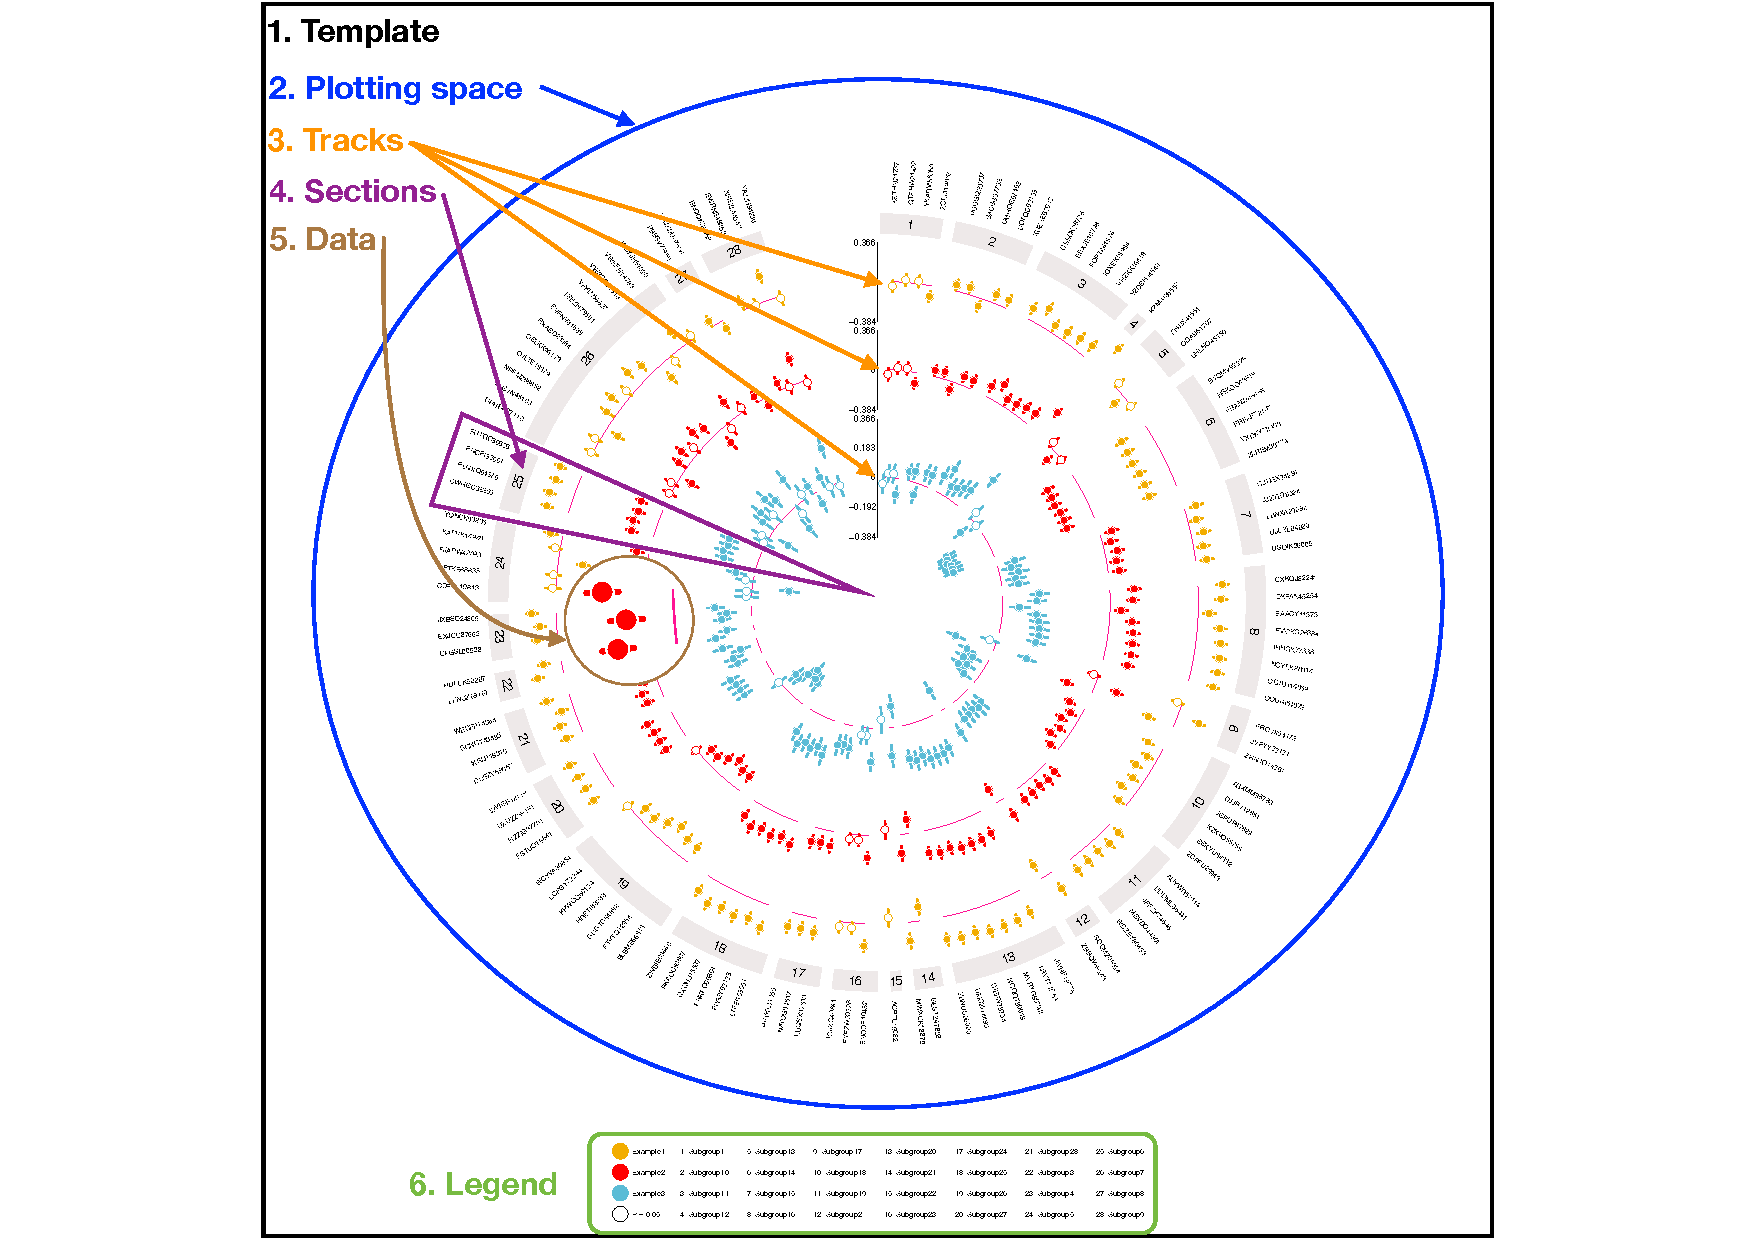
\includegraphics[width=1\linewidth]{data/visualisation/figures/annotated_circos_plot} 

}

\caption[Circos plot highlighting the six elements used to plot data]{\textbf{Circos plot highlighting the six elements used to plot data}. The Circos plot shows three tracks and 28 sections of data simulated to give an example of the effect of three exposures on over 100 outcomes. Available on \href{https://github.com/mattlee821/000_thesis/blob/master/index/data/visualisation/figures/annotated_circos_plot.pdf}{GitHub}.}\label{fig:epiviz-annotated-circos-plot}
\end{figure}
\hypertarget{implementation}{%
\subsection{Implementation}\label{implementation}}

\texttt{EpiViz} is a \texttt{Shiny} web application and \texttt{R} package. \texttt{R}\textsuperscript{\protect\hyperlink{ref-r2019}{501}} version 3.6.2 and \texttt{Shiny}\textsuperscript{\protect\hyperlink{ref-Chang2019}{502}} version 1.4.0 were used to develop the web application; \texttt{R} version 3.6.2 was used to develop the \texttt{R} package. \texttt{Shiny} is an \texttt{R} package that enables the development and deployment of web applications written in the \texttt{R} programming language. Development of \texttt{EpiViz} was progressive and feedback from colleagues was vital in this process.

\par

\hypertarget{operation}{%
\subsection{Operation}\label{operation}}

The \href{https://mattlee.shinyapps.io/EpiViz/}{web application} is publicly accessible and held under an \href{https://github.com/mattlee821/EpiViz/blob/master/LICENSE.txt}{MIT license}. The web application has been tested on computers running macOS (version 10.14) and Windows (version 10) using: Internet Explorer (version 11; Windows), Google Chrome (version 79; macOS and Windows), and Safari (version 13; macOS).

\par

The \href{https://github.com/mattlee821/EpiViz/tree/master/R_package}{\texttt{R} package} is publicly accessible through GitHub and held under an \href{https://github.com/mattlee821/EpiViz/blob/master/LICENSE.txt}{MIT license}. The \texttt{R} package is accessible on all computers with \texttt{R} version 3.3.0 or higher and has been tested on macOS (version 10.14) and Windows (version 10) running \texttt{R} version 3.3.0 or higher.

\par

A legend function is available for both the web application and \texttt{R} package and is implemented using functions from the \texttt{ComplexHeatmap}\textsuperscript{\protect\hyperlink{ref-Gu2016}{500}} \texttt{R} package. By default, the colours used for the Circos plot in both the web application and \texttt{R} package are accessible colours identified using \href{https://medialab.github.io/iwanthue/}{i want hue}. Example data, that I produced, has been provided for users of both the web application and R package. This example data was sourced from Kettunen et al., (2016)\textsuperscript{\protect\hyperlink{ref-Kettunen2016}{335}}, which detailed the effect of body mass index (BMI) on metabolites using Mendelian randomization (MR) using genetic variants associated with BMI in male, female and sex-combined samples. This data is provided on the Home tab on the web application and can be accessed with the \texttt{R} package using the \texttt{EpiViz::EpiViz\_data*()} function, where \texttt{*} is 1-3, specifying data using male (1), female (2), or sex-combined (3) instruments. Example data can be produced for use with the web-application and \texttt{R} package using code on \href{https://github.com/mattlee821/EpiViz/blob/master/R_package/data-raw/example_data_simulation.R}{GitHub}.

\par

\hypertarget{web-application}{%
\subsubsection{Web application}\label{web-application}}

In order to use the \href{https://mattlee.shinyapps.io/EpiViz/}{web application}, a web-browser and an internet connection of at least 1Mbps is required. No other system requirements are needed. Upon opening the web application, users are shown example Circos plots created using simulated and the example data described above, and are directed towards the \emph{Home} tab. The \emph{Home} tab provides users with a short summary of the application, a link to the \texttt{R} package, and example data for use with the app.

\par

The \emph{How to} tab provides instructions for using the application. Step 1 deals with the preparation of data, Step 2 deals with how to use the application, and Step 3 provides information on potential next steps. Users are instructed to upload one data frame per track of the Circos plot. Each data frame should be a tab delimited text file and \texttt{R} code is provided for users to achieve this. The user is guided through an example utilizing the example data of the effect of BMI on metabolites from Kettunen et al., (2016).

\par

Once users have uploaded their data, descriptive information, including a volcano plot (where the effect estimate from the data is shown on the x-axis and p-value on the y-axis), will be produced automatically. Users then select the \emph{Plot} tab, in which they specify the names of the columns in the data for the: label, section, estimate, p-value, lower confidence interval, and upper confidence interval. The estimate, p-value and confidence interval detail the association results provided in the data, the label column details what the user would like to label each association result (e.g., the name of the outcome) and the section column details how the data should be grouped into sections, for example by metabolite class. A p-value adjustment (\(X\)) can be provided to indicate a p-value threshold in the format \(\displaystyle \frac{0.05} {X}\). On the Circos plot, a solid point is indicated as reaching the p-value threshold. An optional legend function is provided and users can choose the labels for the legend points. The legend is auto-populated using the levels in the section column of the uploaded data frame. Finally, an option to use colours accessible to individuals with colour impaired sight is provided.

\par

\hypertarget{r-package}{%
\subsubsection{\texorpdfstring{\texttt{R} package}{R package}}\label{r-package}}

Documentation for using the package is available as a \texttt{README} on \href{https://github.com/mattlee821/EpiViz/tree/master/R_package}{GitHub}. The \texttt{README} includes use cases and troubleshooting. The \texttt{R} package can be installed and loaded into the current \texttt{R} session directly from GitHub with the following code:
\begin{Shaded}
\begin{Highlighting}[]
\CommentTok{\# Install devtools}
\FunctionTok{install.packages}\NormalTok{(}\StringTok{"devtools"}\NormalTok{)}
\FunctionTok{library}\NormalTok{(devtools)}

\CommentTok{\# Install directly from GitHub}
\NormalTok{devtools}\SpecialCharTok{::}\FunctionTok{install\_github}\NormalTok{(}\StringTok{"mattlee821/EpiViz/R\_package"}\NormalTok{)}
\FunctionTok{library}\NormalTok{(EpiViz)}
\end{Highlighting}
\end{Shaded}
\newpage

Once installed, users can use the example data provided with the package to produce Figure \ref{fig:epiviz-figure-example-circos1}, which illustrates the three different types of track available (point, line, bar), using the following \texttt{R} code:
\begin{Shaded}
\begin{Highlighting}[]
\FunctionTok{circos\_plot}\NormalTok{(}\AttributeTok{track\_number =} \DecValTok{3}\NormalTok{,}
            \AttributeTok{track1\_data =}\NormalTok{ EpiViz}\SpecialCharTok{::}\NormalTok{EpiViz\_data1,}
            \AttributeTok{track2\_data =}\NormalTok{ EpiViz}\SpecialCharTok{::}\NormalTok{EpiViz\_data2,}
            \AttributeTok{track3\_data =}\NormalTok{ EpiViz}\SpecialCharTok{::}\NormalTok{EpiViz\_data3,}
            \AttributeTok{track1\_type =} \StringTok{"points"}\NormalTok{,}
            \AttributeTok{track2\_type =} \StringTok{"lines"}\NormalTok{,}
            \AttributeTok{track3\_type =} \StringTok{"bar"}\NormalTok{,}
            \AttributeTok{label\_column =} \DecValTok{1}\NormalTok{,}
            \AttributeTok{section\_column =} \DecValTok{9}\NormalTok{,}
            \AttributeTok{estimate\_column =} \DecValTok{2}\NormalTok{,}
            \AttributeTok{pvalue\_column =} \DecValTok{3}\NormalTok{,}
            \AttributeTok{pvalue\_adjustment =} \DecValTok{1}\NormalTok{,}
            \AttributeTok{lower\_ci =} \DecValTok{4}\NormalTok{,}
            \AttributeTok{upper\_ci =} \DecValTok{5}\NormalTok{,}
            \AttributeTok{lines\_column =} \DecValTok{2}\NormalTok{,}
            \AttributeTok{lines\_type =} \StringTok{"o"}\NormalTok{,}
            \AttributeTok{bar\_column =} \DecValTok{2}\NormalTok{,}
            \AttributeTok{legend =} \ConstantTok{TRUE}\NormalTok{,}
            \AttributeTok{track1\_label =} \StringTok{"Track 1"}\NormalTok{,}
            \AttributeTok{track2\_label =} \StringTok{"Track 2"}\NormalTok{,}
            \AttributeTok{track3\_label =} \StringTok{"Track 3"}\NormalTok{,}
            \AttributeTok{pvalue\_label =} \StringTok{"\textless{}= 0.05"}\NormalTok{)}
\end{Highlighting}
\end{Shaded}



\begin{figure}

{\centering 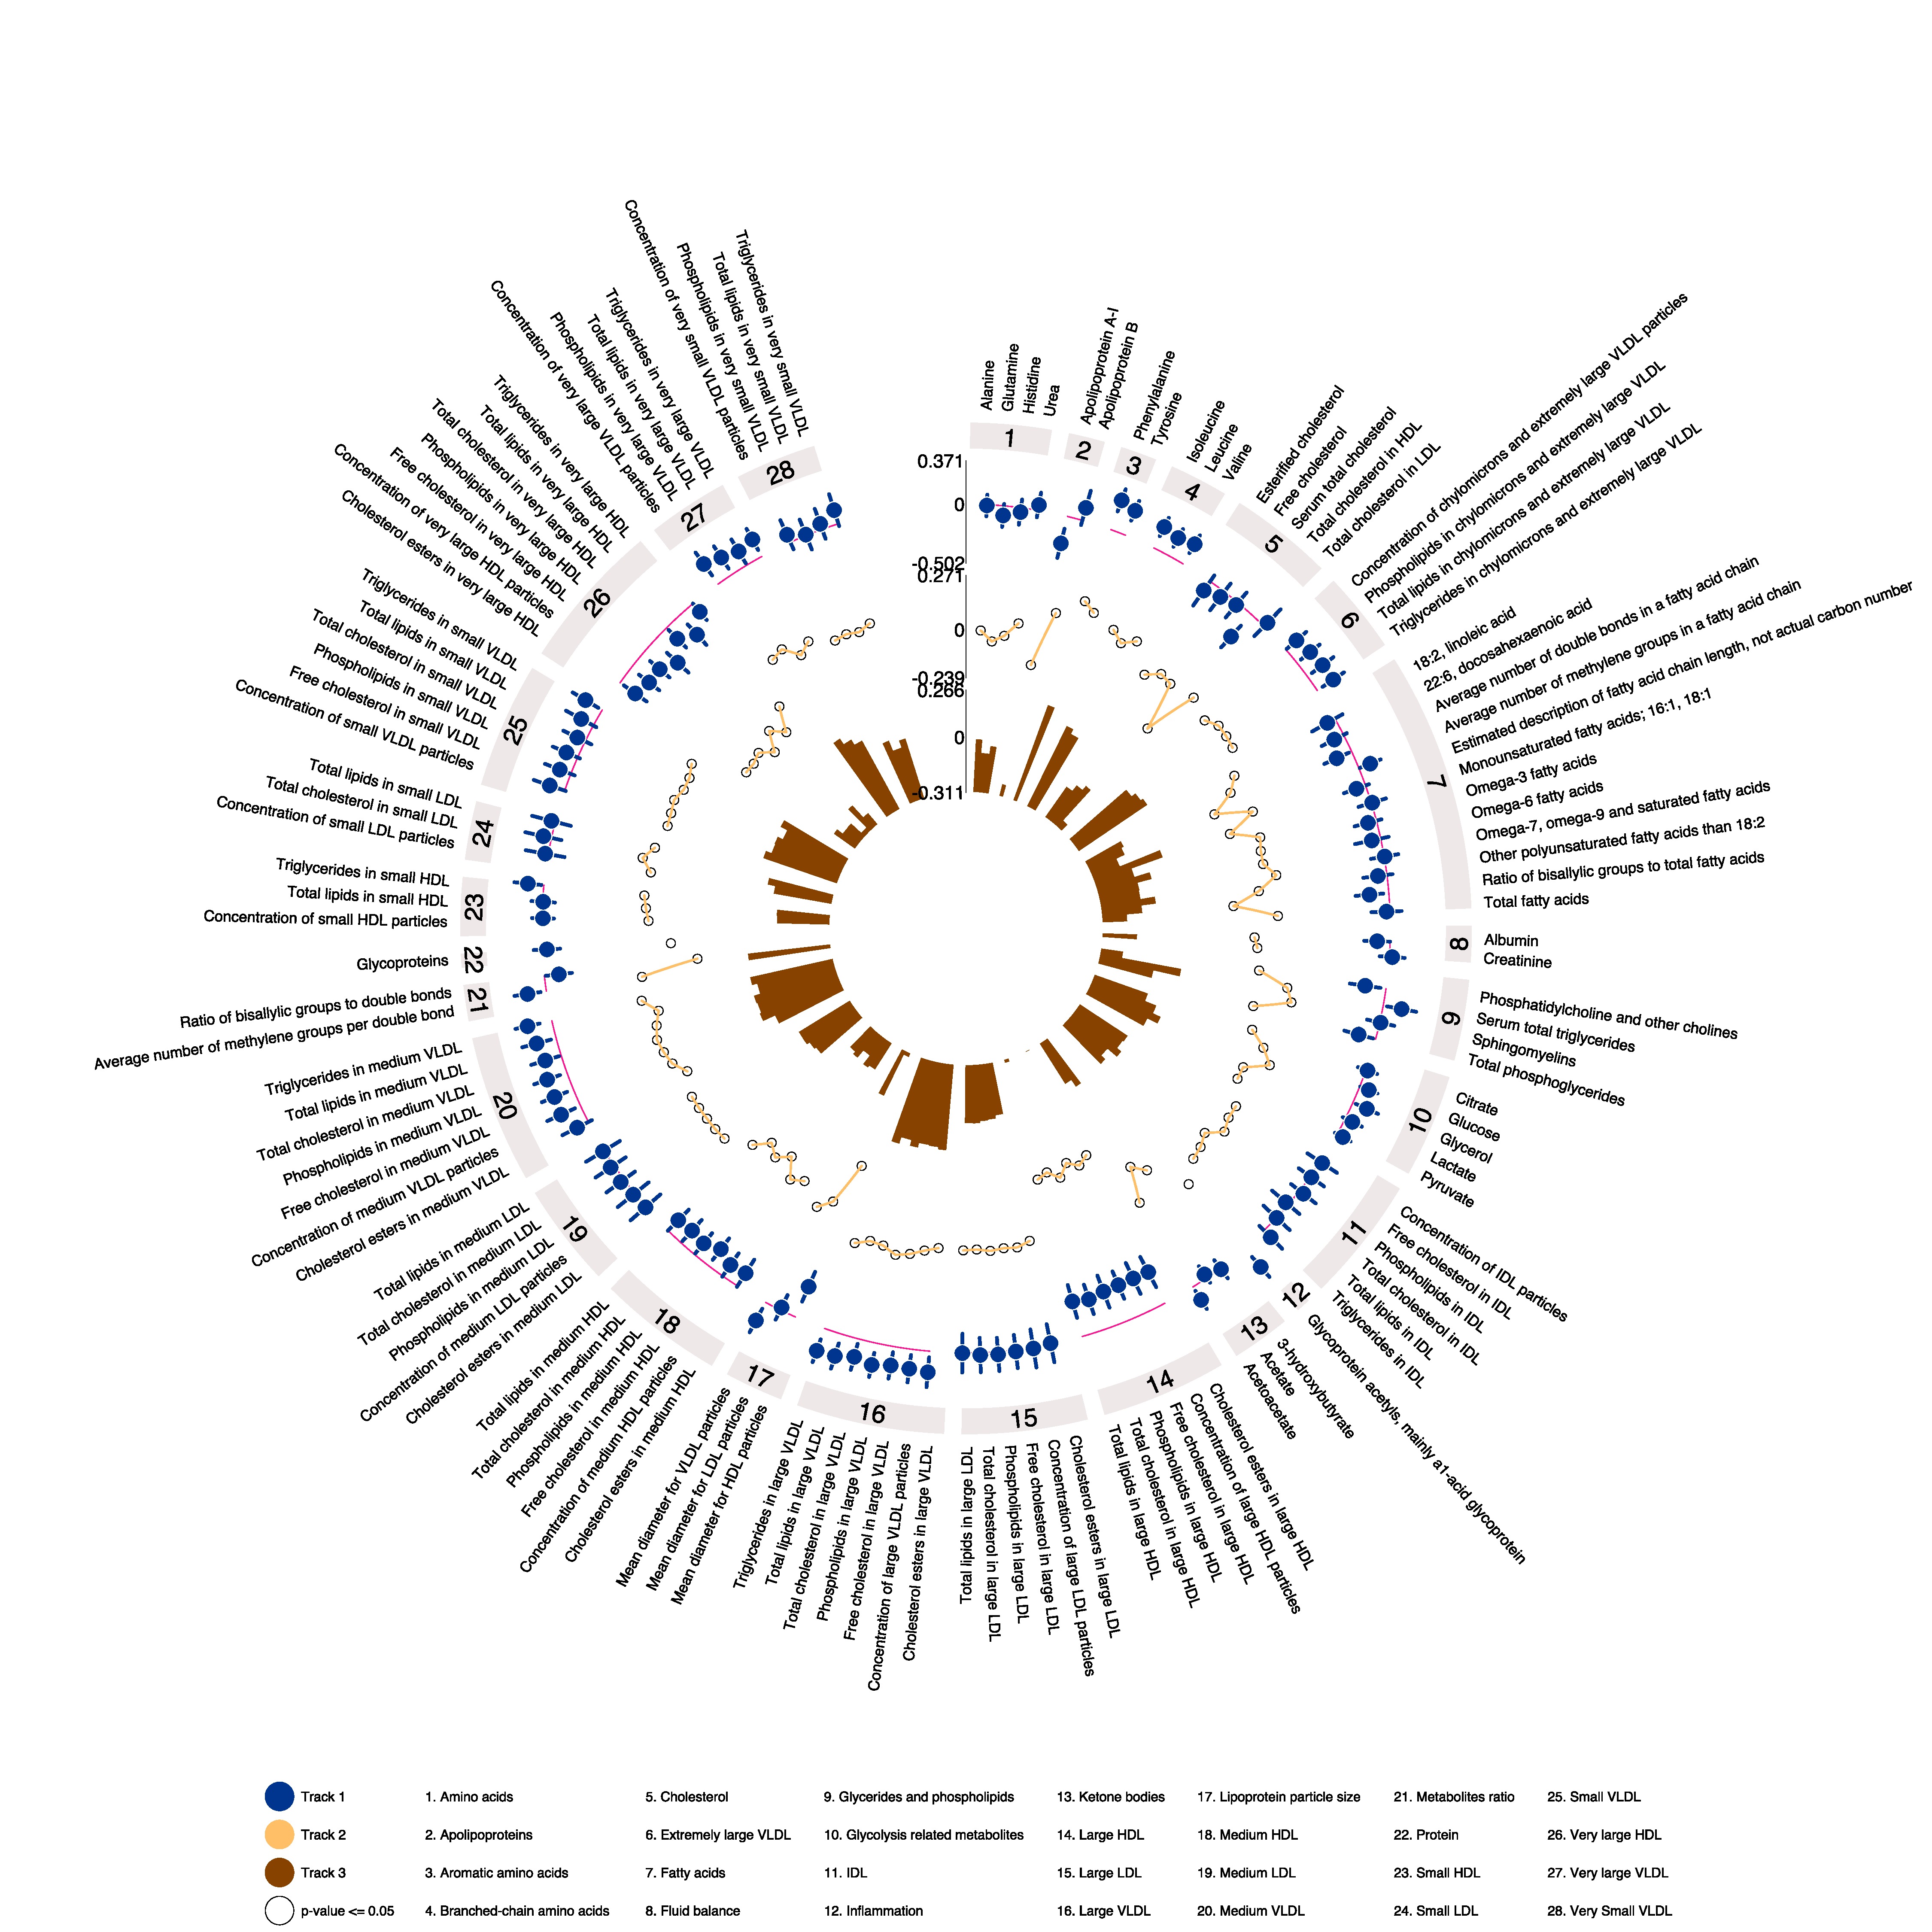
\includegraphics[width=1\linewidth]{data/visualisation/figures/r_package_3_track_type_plot} 

}

\caption[Example Circos plot using \texttt{EpiViz} \texttt{R} package and example data]{\textbf{Example Circos plot using \texttt{EpiViz} \texttt{R} package and example data}. Data presented are results from Mendelian randomization analyses of the association between body mass index and metabolites using data from Kettunen et al., (2016)\textsuperscript{\protect\hyperlink{ref-Kettunen2016}{335}} using male (blue), female (yellow), and sex-combined (brown) instruments from Locke et al., (2015\textsuperscript{\protect\hyperlink{ref-Locke2015}{48}}. Available on \href{https://github.com/mattlee821/000_thesis/blob/master/index/data/visualisation/figures/r_package_3_track_type_plot.pdf}{GitHub}.}\label{fig:epiviz-figure-example-circos1}
\end{figure}
In producing plots using the \texttt{R} package, users are advised to save as \texttt{PDF} using the below code. This is because the Circos plot is designed to be larger than normal plots, as such viewers like the \texttt{R} Studio Viewer pane display the plot in a compressed form, squashing the plot. Viewers like this should be used only as a guide when making the plot. \texttt{PDF} files can be converted to other image formats without compression. Users are advised to iterate the sizing of the plot, adjusting the width and height arguments to get the desired plot size and then adjust the point size argument to increase and decrease the size of the information in the plot (labels, points, lines, etc.). The values provided in the below code work with most plots and were used for all examples in this Chapter. In addition, users can adjust the size of the Circos plot directly using the argument \texttt{circle\_size}. The default for \texttt{circle\_size} is 25, smaller numbers increase the size of the circle and larger numbers decrease the size of the circle:
\begin{Shaded}
\begin{Highlighting}[]
\FunctionTok{pdf}\NormalTok{(}\StringTok{"my\_circos\_plot.pdf"}\NormalTok{,}
    \AttributeTok{width =} \DecValTok{30}\NormalTok{, }\AttributeTok{height =} \DecValTok{30}\NormalTok{, }\AttributeTok{pointsize =} \DecValTok{35}\NormalTok{)}
\FunctionTok{circos\_plot}\NormalTok{(...}
            \AttributeTok{circle\_size =} \DecValTok{25}\NormalTok{)}
\FunctionTok{dev.off}\NormalTok{()}
\end{Highlighting}
\end{Shaded}
Finally, users can adjust the height of tracks individually using \texttt{track*\_height} where \texttt{*} refers to the track number. The default for each track is 20 percent of the total size of the circle, the section track is fixed at 5 percent of the total size of the circle. The remaining space is at the centre of the circle. Tracks can be increased in size to occupy more, or less, of the circles size using the following arguments:
\begin{Shaded}
\begin{Highlighting}[]
\FunctionTok{circos\_plot}\NormalTok{(...}
            \AttributeTok{track1\_height =} \FloatTok{0.2}\NormalTok{,}
            \AttributeTok{track2\_height =} \FloatTok{0.2}\NormalTok{,}
            \AttributeTok{track3\_height =} \FloatTok{0.2}\NormalTok{)}
\end{Highlighting}
\end{Shaded}
In order to minimise the time required to maintain the \texttt{R} package, further customisation is achieved by the users themselves. The function is written to aid this customisation with \emph{Default parameters} and \emph{Customisable parameters} located at the top of the \texttt{circos\_plot()} function. Guidance and code is provided on \href{https://github.com/mattlee821/EpiViz/tree/master/R_package}{GitHub} to aid user customisation.

\par

\hypertarget{discussion}{%
\section{Discussion}\label{discussion}}

Circos plots have been used to visualise and provide overview of large metabolomic association analyses\textsuperscript{\protect\hyperlink{ref-Bos2021}{1},\protect\hyperlink{ref-Shin2014}{334},\protect\hyperlink{ref-Kettunen2016}{335},\protect\hyperlink{ref-Taylor2019}{490},\protect\hyperlink{ref-Kettunen2012}{498}}. When creating Circos plots for Taylor et al.~(2019)\textsuperscript{\protect\hyperlink{ref-Taylor2019}{490}}, the process was cumbersome and inefficient with each revision requiring me to write bespoke code. \texttt{EpiViz} simplifies and streamlines the process of making Circos plots. In Bos et al.~(2021)\textsuperscript{\protect\hyperlink{ref-Bos2021}{1}}, \texttt{EpiViz} was used to summarise and visually compare observational and Mendelian randomization analyses of multiple sleep traits on over 100 metabolites. \texttt{EpiViz} made producing and refining Circos plots for this analysis faster and more efficient.

\par

The web application is intended for researchers with limited to no experience of \texttt{R} and is in a stable release. Additions to the web applications functionality are therefore not envisioned. The \texttt{R} package, also in a stable release, will be the focus of further development as maintenance costs are lower as there is no requirement for the additional coding of the user interface as with the web application. The focus of future changes should be on converting the current code style to the \href{https://tidyverse.tidyverse.org/articles/manifesto.html}{\texttt{tidy} style} to improve readability and consistency. This will also improve the ease with which contributions can be implemented. Additional features should be directed by the needs of the users, this is likely to include additional plotting mechanics such as the chord diagram, which shows relatedness between nodes. In the case of metabolites, a chord diagram would provide greater understanding about the relationship between different sections and individual metabolites. In addition, the ability to filter and choose specific sections to display would simplify the presentation of key results -- currently this is achieved with supplementary forest plots.

\par

In order to achieve the desired goal of providing global overview of large association analyses, Circos plots are larger than traditional plots. This poses a challenge for their use in print as there are size restrictions. Circos plots are therefore ideally suited to online use, however, if large enough, and with proper sizing of text, they can be used as overview figures in printed media. When used online there is the potential for creating interactive Circos plots, allowing users to expand and filter the Circos plot as desired. Interactive plots can be used in online publications such as \href{https://blog.f1000.com/2017/07/19/so-long-static-we-now-support-interactive-ploty-figures-in-our-articles/}{F1000} which encourage use of the \texttt{plotly} \texttt{R} package for interactive figures. This can enhance the reader experience, allowing readers to gain a better understanding of the presented research.

\par

For this thesis, the effect of adiposity on metabolites as a whole and as subclasses, i.e., profiles, is key to interpreting the effects of adiposity. This is because metabolites are highly inter-correlated and perturbations rarely happen in isolation. The ability to visualise these profiles can therefore aid the interpretation of the global effects of adiposity as well as provide context for the effect of adiposity on an individual metabolite. Forest plots can provide this overview, however the need for many, or very long, plots makes summarising results challenging and visually unappealing. Circos plots, while remaining visually appealing, are able to visualise a far greater number of results and maintain their ability to provide global overview.

\par

\texttt{EpiViz} is simple and efficient to use. The web app provides a platform for quick and simple plots to be generated while the \texttt{R} applicaton provides customisation. \texttt{EpiViz} has been successfully used to interrogate large metabolomic association analyses\textsuperscript{\protect\hyperlink{ref-Bos2021}{1},\protect\hyperlink{ref-Taylor2019}{490},\protect\hyperlink{ref-Bell2020}{491}} and will be used throughout this thesis to achieve the same goals.

\par

\newpage

\hypertarget{observational}{%
\chapter{Associations between multiple measures of adiposity and metabolites: observational analysis}\label{observational}}

\hypertarget{chapter-summary-3}{%
\section*{Chapter Summary}\label{chapter-summary-3}}
\addcontentsline{toc}{section}{Chapter Summary}

In Chapters \ref{introduction} and \ref{systematic-review}, the link between adiposity and disease from existing literature was presented in observational and causal analysis frameworks. This work highlighted that adiposity is associated, likely causally, with many outcomes. A key takeaway from Chapter \ref{introduction} was that the underlying mechanisms of disease development are not well understood, but that some relationships between adiposity and disease may be explained by changes in metabolic pathways. In this Chapter, observational epidemiological methods are used to explore associations between adiposity and metabolites. The aim of this Chapter is to provide an observational grounding for subsequent causal analysis work in Chapters \ref{MR} and \ref{mediation}, and is the first of two analyses that will assess the same question with different study designs (i.e., triangulation) with the next study design presented in Chapter \ref{MR}.

\par

\newpage

\hypertarget{observational-intro}{%
\section{Introduction}\label{observational-intro}}

Adiposity is associated with an increased risk of numerous diseases, as well as mortality\textsuperscript{\protect\hyperlink{ref-Pischon2008}{82},\protect\hyperlink{ref-Flegal2013}{86}--\protect\hyperlink{ref-Elagizi2018}{88},\protect\hyperlink{ref-Jenkins2018}{100}--\protect\hyperlink{ref-Bigaard2004}{105}} (see Chapters \ref{introduction} and \ref{systematic-review}). There is a need to understand the mechanisms underlying these associations so that intervention strategies, which are challenging to implement effectively, can be targeted and more efficacious.

\par

Adiposity has been linked with many downstream measures that could serve as intermediates of disease and thus be useful targets for reducing the burden of adiposity. Notably, as adiposity has been associated with many metabolites\textsuperscript{\protect\hyperlink{ref-Wurtz2014}{286},\protect\hyperlink{ref-Cirulli2019}{287},\protect\hyperlink{ref-Moore2014}{345},\protect\hyperlink{ref-SantosFerreira2017}{386}--\protect\hyperlink{ref-Stevens2020}{389},\protect\hyperlink{ref-Wulaningsih2019}{391}--\protect\hyperlink{ref-Rangel-Huerta2019}{395}}, previous work has highlighted metabolites\textsuperscript{\protect\hyperlink{ref-Collaboration2009}{99},\protect\hyperlink{ref-Bray2004}{294},\protect\hyperlink{ref-Haslam2005}{295}} as a possible link between adiposity and diseases such as cancer\textsuperscript{\protect\hyperlink{ref-Bhaskaran2014}{120}}, coronary heart disease (CHD)\textsuperscript{\protect\hyperlink{ref-Paul2006}{134},\protect\hyperlink{ref-Koliaki2019}{135}}, and type 2 diabetes\textsuperscript{\protect\hyperlink{ref-Al-Goblan2014}{171}}. In the largest study to date by Wurtz et al., (2014)\textsuperscript{\protect\hyperlink{ref-Wurtz2014}{286}}, adiposity was found to influences whole classes of metabolites including amino acids, fatty acids, hormones, inflammatory markers, and lipids. Metabolites are intermediate or end products of cellular processes with multiple functions including those with energy, signalling, transportation, and structural components. Metabolic effects can be far reaching\textsuperscript{\protect\hyperlink{ref-Wishart2019}{328},\protect\hyperlink{ref-Johnson2016}{329}} and during homeostasis are tightly controlled. The many functions metabolites have mean that imbalances can be detrimental\textsuperscript{\protect\hyperlink{ref-Griffin2006}{325},\protect\hyperlink{ref-Wishart2019}{328},\protect\hyperlink{ref-Johnson2016}{329}}.

\par

Measurement of metabolites has become increasingly common among cohort studies with mass spectrometry (MS) and nuclear magnetic resonance (NMR) platforms able to perform targeted, semi-targeted, and untargeted assays. Although there is evidence to show the relationship between adiposity and metabolites varies between sexes and over time\textsuperscript{\protect\hyperlink{ref-Wurtz2014}{286}}, the focus of many analyses has been on body mass index (BMI) as a measure for overall adiposity, has included small sample sizes, and has looked at a single time-point. While BMI correlates well with, and is a predictor of, many health outcomes\textsuperscript{\protect\hyperlink{ref-Donato1998}{72},\protect\hyperlink{ref-NIH2013}{73}}, it is a crude measure of adiposity with several issues, not least the inability to differentiate lean and fat mass\textsuperscript{\protect\hyperlink{ref-Flegal2009}{75}}. Evidence highlights the importance and utility of combining complimentary measurements of adiposity\textsuperscript{\protect\hyperlink{ref-WorldHealthOrganisation2008}{94},\protect\hyperlink{ref-Collaboration2009}{99}}. As many studies have focussed on the effect of adiposity on metabolites in adulthood and given the effects of adiposity are shown to present early in life\textsuperscript{\protect\hyperlink{ref-Bibbins-Domingo2007}{503}--\protect\hyperlink{ref-Biro2010}{507}}, there is a need to understand how and importantly when, adiposity-related metabolites may be of most use in reducing the burden of adverse health outcomes. Investigation of the effects of adiposity over time may therefore provide additional information on the relationship between adiposity and metabolites.

\par

The Avon Longitudinal Study of Parents and Children (ALSPAC), a longitudinal birth cohort study, with repeated metabolomic and anthropometric measures, provides an opportunity to expand on the current literature. In this Chapter, observational analysis assessing the association between multiple measures of adiposity and NMR derived metabolites provide a basis from which to investigate causality with a triangulation approach.

\par

\hypertarget{observational-methods}{%
\section{Methods}\label{observational-methods}}

\hypertarget{overview}{%
\subsection{Overview}\label{overview}}

This chapter details hypothesis-free, linear regression analyses that, cross-sectionally, aimed to identify signals of association between measures of adiposity and NMR-derived metabolites at multiple time-points in ALSPAC. Data were available from ALSPAC for exposures (measures of adiposity), outcomes (metabolites), and covariables. Exposures included BMI, waist hip ratio (WHR) and body fat percentage (BF). Metabolomic data were available for up to 234 NMR derived metabolites. These, predominantly lipid-based, metabolites include directly measured metabolites such as the amino acids tyrosine and phenylalanine, as well as derived (not-directly measured) metabolite measures such as the ratio of saturated fatty acids to total fatty acid. Throughout, ``metabolites'' is used to refer to both directly measured and derived (not-directly measured) measures, otherwise they are referred to as ``directly measured metabolites'' and ``derived'' or ``not-directly measured metabolites'' respectively.

\par

Covariables included age, sex, mother's or own education, smoking history, alcohol history, diet, and physical activity. Covariables were chosen as evidence has shown an association between them and adiposity and metabolites. All data were pre-exisiting, that is I did not collect this data. All analyses and data manipulation were performed using \texttt{R} (version 3.6.2)\textsuperscript{\protect\hyperlink{ref-r2019}{501}}. Specific \texttt{R} packages are described, where appropriate. All code for this work is available on \href{https://github.com/mattlee821/000_thesis/tree/master/index/data/observational}{GitHub}.

\par

\hypertarget{data-overview}{%
\subsection{Data overview}\label{data-overview}}

ALSPAC\textsuperscript{\protect\hyperlink{ref-Fraser2013}{508}--\protect\hyperlink{ref-Northstone2019}{510}} is a prospective cohort study that invited women resident in Avon, UK with expected dates of delivery between 1st April 1991 and 31st December 1992 to participate. The initial number of pregnancies enrolled was 14,541 (for these at least one questionnaire was returned or a ``Children in Focus'' clinic has been attended by 19/07/99). Of these initial pregnancies, a total of 14,676 foetuses, resulted in 14,062 live births and 13,988 children alive at one year of age. The mothers and fathers associated with each pregnancy are referred to as generation 0 (G0) while the children of each eligible pregnancy (including individuals from subsequent recruitment drives) are referred to as generation 1 (G1).

\par

When the oldest G1 individuals were approximately seven years of age, an attempt was made to bolster the initial sample with eligible cases who had failed to join the study originally. As a result, when considering variables collected from the age of seven onwards (and potentially abstracted from obstetric notes), there are data available for more than the 14,541 pregnancies mentioned above. The number of new pregnancies not in the initial sample (known as Phase I enrolment) that are currently represented on the built files and reflecting enrolment status at the age of 24 is 913 (456, 262, and 195 recruited during Phases II, III, and IV respectively), resulting in an additional 913 G1 individuals being enrolled. The phases of enrolment are described in more detail in the cohort profile paper and its update\textsuperscript{\protect\hyperlink{ref-Fraser2013}{508}--\protect\hyperlink{ref-Northstone2019}{510}}. The total sample size for analyses using any data collected after the age of seven is therefore 15,454 pregnancies, resulting in 15,589 foetuses, of which 14,901 were alive at one year of age.

\par

The study \href{http://www.bristol.ac.uk/alspac/}{website} contains details of all the data that is available through a fully searchable data dictionary and \href{http://www.bristol.ac.uk/alspac/researchers/our-data/}{variable search tool}. Ethical approval for the study was obtained from the ALSPAC Ethics and Law Committee and the \href{http://www.bristol.ac.uk/alspac/researchers/research-ethics/}{Local Research Ethics Committees}. Informed consent for the use of data collected via questionnaire and clinics was obtained from participants following recommendations of the ALSPAC Ethics and Law Committee at the time. Full details of the ALSPAC consent procedures are available on the \href{http://www.bristol.ac.uk/alspac/researchers/research-ethics/}{study website}.

\par

Data in ALSPAC are split by clinic visits. For this work, metabolomic data were available for G1 individuals from the following clinics: Focus at 7 (\textasciitilde8 years old), Focus at 8 (\textasciitilde9 years old), Before Breakfast Study (\textasciitilde8 years old), Teen Focus 3 (\textasciitilde18 years old), Teen Focus 4 (\textasciitilde17 years old), and Focus at 24 (\textasciitilde24 years old). Metabolomic data for G0 individuals were available from: Focus on Mothers 1 (\textasciitilde48 years old), Focus on Mothers 2 (\textasciitilde51 years old), and Focus on Fathers 1 (\textasciitilde53 years old). In order to maximize the sample size at each metabolomic clinic, data were combined where clinics were within a similar age range. Data were combined in the following groups for G1 individuals: Focus at 7 and Before Breakfast Study (children), and Teen Focus 3 and Teen Focus 4 (adolescents). The Focus at 24 clinic is referred to as young adults. For G0 individuals data from Focus on Mothers 1, Focus on Mothers 2, and Focus on Fathers 1 were combined into an adults group. For these combined data sets, duplicate individuals (i.e., those attending both clinics) were identified, and the measurement from the most recent clinic was dropped.

\par

All data on exposures and covarialbes were obtained from the same clinic from which metabolomic data were collected. Where data on exposures and covarialbes were not available at the metabolomic clinic visit, they were obtained from the most recent clinic with available data. The Before Breakfast Study, unlike the other clinics, only collected metabolomic data, as such data on exposures and covarialbes were extracted for these individuals from the Focus at 8 clinic. Metabolomic data for each time point were extracted first and subsequent data on exposures and covarialbes were extracted for individuals with metabolomic data. The metabolomic data were provided with standard exclusions for identifiable individuals and those with withdrawn consent already excluded.

\par

The aim of this analysis was to look cross-sectionally across multiple time points at the association between adiposity measures and metabolites. It is important to note that, although G0 and G1 individuals were independent, there is familial overlap between them. Additionally, G1 individuals were not independent, that is, the same individuals will have attended multiple clinics. As such, any effects specific to an individual may be propagated through all G1 clinics that individual attends.

\par

\hypertarget{observational-methods-exposures}{%
\subsection{Exposures: adiposity}\label{observational-methods-exposures}}

Measures of adiposity (BMI, WHR, and BF) were obtained for all individuals with available metabolomic data. Data on WHR was not available for the Teen Focus 3 and 4 clinics. BMI was calculated as \(\displaystyle \frac{weight(kg)}{height (m^2)}\) and WHR as \(\displaystyle \frac{waist\ circumference\ (cm)} {hip\ circumference\ (cm)}\). Height was measured once to the last complete mm using the Harpenden Stadiometer. Individuals were positioned with their feet flat and heels together, standing straight so that their heels, calves, buttocks and shoulders came into contact with the vertical backboard of the stadiometer. The headboard was lowered until it touched the individual's head and a 1kg weight was placed on the headboard to ensure head contact and to minimise hair thickness. Weight was measured once using the Tanita Body Fat Analyser (Models TBF 305 and 401A) or electronic bathroom scales, if the individual had a pacemaker. Individuals were encouraged to pass urine and undress to their underclothes. Individuals stepped onto the measuring platform which had been wiped with disinfecting alcohol and positioned so that both feet were located in parallel with the toe and heel in contact with their respective electrodes. Measurement was completed when the weight and fat ratio readings were fixed and the buzzer beeped. Weight was measured to the nearest 50g for G1 individuals and to the nearest 0.1kg for G0 individuals. For all G1 individuals, `Female Standard' was entered into the Tanita Body Fat Analyser as the sex variable. Circumferences were measured using the Seca 200 or 201 body tension tape and were repeated twice for accuracy.

\par

BF was measured using dual-energy x-ray absorptiometry (DXA) in all individuals except for individuals from Focus at 7. Briefly, measurement required individuals to be prone and stationary while a Lunar prodigy narrow fan beam densitometer performed a whole body DXA scan. Data were processed using Lunar Prodigy software. Individuals did not have measurements taken if they: were pregnant, had a radiological investigation using contrast media within the week before the DXA scan, had a recent nuclear medicine investigation with persistent radioactivity or weighed greater than 159kg. BF was calculated as \(\displaystyle \frac{fat\ mass} {fat\ mass + fat\ free\ mass}\ *\ 100\).

\par

For Focus at 7, BF was not measured, instead bioeletrical impedance data, which were converted to estimates of BF, were available. Briefly, individuals were encouraged to pass urine and undress to their underclothes. A Tanita Body Fat Analyser (Model TBF 305) was used to measure weight and impedance. Height was entered to the nearest cm and `Female Standard' was used as the sex variable for all individuals. The Tanita Body Fat Analyser TBF 305 is a single frequency (50kHz) leg-to-leg device. In single frequency devices, impedance is a representation of resistance which is related to the volume of water (which one assumes makes up the majority of fat free mass (FFM)), as such, the higher the resistance (impedance) the greater the amount of FFM. Calculation of BF from the impedance measure is only possible at the time of measurement, however these derived BF measures were not stored and the equation to calculate them was not available from the manufacturer. Previous work\textsuperscript{\protect\hyperlink{ref-Chouinard2007}{97}} has shown that comparison of BF derived from the manufacturer's equation and an alternative\textsuperscript{\protect\hyperlink{ref-Jebb2000}{96}} showed little difference in resulting BF estimates. The alternative equation was derived in a study involving 205 (101 women) healthy adults with a mean age of 43.8 (SD = 16) for men and 40.4 (SD = 13.6) for women. The alternative equation, where \(Z\) is the impedance measure from the device in ohms, height is in metres, weight is in kilograms, age is in years, and female-specific components are given as \(19.6\ +\ ln(height)\), is given as:

\par
\begin{equation}
\begin{split}
  BF = -156.1 - 89.1\ ln(height) \\
  \ +\ 45.6\ ln(weight) \\
  \ +\ 0.120\ age\ \\
  \ +\ 0.0494\ Z \\
  \ +\ (19.6\ ln(height))
\end{split}
  \label{eq:BF}
\end{equation}
Given that the equation was derived from adult data, its application to child data in ALSPAC was explored in this Chapter. A raw impedance measure, from a similar model (Tanita Body Fat Analyser (Model TBF 401A)), was obtained for individuals from Teen Focus 3 and 4 (i.e., where both DXA and impedance measures were available) and the equation was used to compare BF derived from the impedance device and BF measured with DXA in adolescents. Exploration involved visual inspection of distribution and Spearman's correlation with BMI, height, weight and other BF measures from Teen Focus 3 and 4. The same observations were carried out for raw impedance. The calculated BF estimates were positively correlated with height and weight, however there were negative values of calculated BF. As the estimates derived in linear models are in reference to the per unit increase in an exposure (rather than the range), the absolute value of the exposure does not need to positive. Thus, the negative estimates of BF will not impact the inference of a linear regression between BF and any metabolite. As such, BF calculated using equation \eqref{eq:BF} was used in subsequent analyses as a measure of BF in children.

\par

\hypertarget{outcomes-metabolites}{%
\subsection{Outcomes: metabolites}\label{outcomes-metabolites}}

Metabolomic data were measured using the same NMR platform for all individuals. Briefly, high-throughput proton (\textsuperscript{1}H) NMR assays were performed on ethylenediaminetetraacetic acid (EDTA) plasma/serum samples. Samples were fasted. Measurements were taken at three molecular windows (lipoprotein lipids, low molecular-weight metabolites, and lipid extracts) enabling broad quantification of metabolomic measures. These measures also included derived measures, lipoprotein particle sizes, and fatty acid ratios, inclusion of which has shown to increase overall power in statistical analyses\textsuperscript{\protect\hyperlink{ref-Altmaier2008}{511}--\protect\hyperlink{ref-Suhre2010}{513}}. Metabolite values for each individual were provided by the NMR platform in the originally measured units (e.g., mmol/l). Derived metabolite values are as a \%. Full details on the NMR methodology has previously been described\textsuperscript{\protect\hyperlink{ref-Kettunen2012}{498},\protect\hyperlink{ref-Soininen2009}{514}--\protect\hyperlink{ref-Soininen2015}{516}} and is available from the \href{http://www.bristol.ac.uk/alspac/researchers/access/}{ALSPAC data dictionary} (data dictionary identifiers: children = D5704, mothers = D5705, fathers = D5700). The Before Breakfast study does not have a documentation file and is described elsewhere\textsuperscript{\protect\hyperlink{ref-Ong2004}{517}}; fasted metabolomic data, not the post glucose challenge metabolomic data, were taken from The Before Breakfast Study. Descriptions of metabolites are available on \href{https://github.com/mattlee821/000_thesis/blob/master/index/data/observational/tables/metabolites.txt}{GitHub}.

\par

The spectral NMR data were processed by Nightingale Health and provided by the ALSPAC team as a processed file with identifiable individuals (triplets/quadruplets) and individuals who had withdrawn consent removed. Some mothers and fathers were duplicated in this data due to the way in which mothers were originally enrolled into the study and assigned IDs. If a mother enrolled with two different pregnancies (both having an expected delivery date within the recruitment period (April 1991-December 1992)), she will have two separate IDs. A father associated with both of these pregnancies will also be duplicated. Duplicate measurements for mothers and fathers were removed. No metabolites were excluded at this stage, however the number of metabolites available for each clinic visit differed as metabolites were added and removed over time by Nightingale as validations change.

\par

Pre-analysis processing of metabolomic data is important as there can be quality issues with sample and metabolite data\textsuperscript{\protect\hyperlink{ref-Hughes2021}{518}}. However, there is no standardised method for performing pre-analysis processing and for deciding what thresholds to use to exclude metabolites and individuals from downstream analyses. The \texttt{R} package \href{https://github.com/MRCIEU/metaboprep}{\texttt{metaboprep}}\textsuperscript{\protect\hyperlink{ref-Hughes2021}{518}} can be used to process data before analyses using a transparent and reproducible workflow. Here, after combining clinic visit data, where appropriate, \texttt{metaboprep} (version 0.0.1) was used to identify and exclude individuals and metabolites that did not meet certain requirements. This process was performed twice, firstly including and secondly excluding the derived metabolomic measures from missingness and clustering analyses to see if these derived measures were unduly influencing exclusions. Briefly, individuals and then metabolites, with high missingness (\(\geq\) 80\%) were removed. Missingness was then re-calculated for individuals and metabolites, with removal based on 20\% missingness. Individuals were then removed based on total sum abundance, considering outliers as \(\geq\) 5 standard deviations (SD) away from the mean. Using this metabolite dataset, a dendrogram using complete-linkage and a Spearman's rho distance matrix was produced, and a set of clusters identified based on a Spearman's rho of 0.5. For each cluster, the metabolite with the least missingness was tagged as the representative feature. Finally, principal component (PC) analysis was conducted using the representative features to evaluate structure among individuals. Outliers were identified as being \(\geq\) 5 SDs away from the mean of PC 1 and 2, and were excluded. Additionally, in order to gain an overview of the variability of metabolite concentrations, the mean, SD of the mean, median, and range of metabolite concentrations were visually compared across age groups.

\par

\hypertarget{covariables}{%
\subsection{Covariables}\label{covariables}}

Evidence has shown that age\textsuperscript{\protect\hyperlink{ref-Yu2012}{519},\protect\hyperlink{ref-Brennan2020}{520}}, sex\textsuperscript{\protect\hyperlink{ref-Brennan2020}{520}}, education\textsuperscript{\protect\hyperlink{ref-Zajacova2018}{521}}, smoking\textsuperscript{\protect\hyperlink{ref-Bonevski2014}{522}}, alcohol\textsuperscript{\protect\hyperlink{ref-Bonevski2014}{522}}, diet\textsuperscript{\protect\hyperlink{ref-Afshin2019}{523}}, and physical activity\textsuperscript{\protect\hyperlink{ref-ODonoghue2018}{524}} all influence the metabolomic profile and adiposity. Data for each of these covarialbes were obtained for all individuals with metabolomic data. Age was taken from the metabolomic clinic visit as months since birth. Sex was taken from the initial assessment questionnaire for G1 individuals completed by their parents. For G0, an individual's sex was as self-reported at the metabolomic clinic visit.

\par

Maternal education was used as an adjustment for children, adolescents and young adults. Own education was used for mothers and mother-reported partner education was used for fathers. Specifically, mothers were asked, during their pregnancy, `What educational qualifications do you, your partner, your mother, and your father have?' with possible answers: CSE or GCSE (D, E, F or G); O-level or GCSE (A, B, or C); A-level; qualifications in shorthand/ typing/or other skills e.g.~hairdressing;, apprenticeship; state enrolled nurse; state registered nurse; City and Guilds intermediate technical; City \& Guilds final technical; City \& Guilds full technical; teaching qualification; university degree; no qualification; qualifications not known; not applicable; or other (please describe). This data was available as a recoded variable of 5 categories of lowest (1) to highest (5) level of education.

\par

The variable capturing smoking was binary; adolescents (at the metabolomic clinic), young adults (at the metabolomic clinic), and adults (mothers were asked during pregnancy; fathers were asked at a clinic prior to the metabolomic clinic) were asked whether they had ever smoked a cigarette before.

\par

Alcohol was assessed differently for Teen Focus 3 and Teen Focus 4, Focus at 24, and G0 individuals. Individuals from Teen Focus 3 were asked what their alcohol drinking pattern was with possible answers: only ever tried drinking once/twice, used to drink sometimes {[}but{]} never drink now, sometimes drink but less than once a week, usually drink on 1 or 2 days a week, usually drink on \textgreater2 days a week but not every day, and usually drink every day. Individuals from Teen Focus 4, Focus at 24, and G0 individuals (mothers were asked at a prior clinic visit to the metabolomic clinic and fathers at the metabolomic clinic) were asked the frequency they had drinks containing alcohol with possible answers: never, monthly or less, two to four times a month, two to three times a week, four or more times a week.

\par

Diet data derived by Anderson et al., (2013)\textsuperscript{\protect\hyperlink{ref-Anderson2013}{525}} were available for G1 individuals aged 7 and 13. Data from age 7 was matched with metabolomic data for Focus at 7 while data from age 13 was matched with metabolomic data for Teen Focus 3 and 4. Diet data were not available for young adults or adults. Data is given as predicted kilo-calories consumed per day.

\par

Data on physical activity were collected differently for different clinic visits. For G1 individuals from Teen Focus 3 and Focus at 24, accelerometry data were collected at the same clinic at which metabolomic data were collected. Briefly, individuals wore an accelerometry device for the 7 days following their clinic visit whilst keeping a diary of the times they wore and took off the device. Individuals were advised to wear the accelerometer device if the following days were part of a `normal week' with regards to their activity. For Focus at 24 individuals, physical activity data were the average number of minutes per day spent doing moderate to vigorous physical activity. For Teen Focus 3 individuals, physical activity data were the mean counts per minute spent doing moderate to vigorous physical activity for the whole week. For G0, individuals were asked `Do you take part in physical activity (e.g., running, swimming, dancing, golf, tennis, squash, jogging, and bowls)?' with possible answers: no, occasionally (less than monthly), and frequently (once a month or more). Data for mothers were available in a clinic prior to the metabolomic clinic, fathers data were available at the metabolomic clinic. Physical activity data were not available for Focus at 7.

\par

\hypertarget{statistical-analysis}{%
\subsection{Statistical analysis}\label{statistical-analysis}}

Metabolomic data were available for: Focus at 7 (n = 5518; metabolites = 230), Before Breakfast Study (n = 640; metabolites = 228), Teen Focus 3 (n = 3371; metabolites = 230), Teen Focus 4 (n = 3175; metabolites = 230), Focus at 24 (n = 3269; metabolites = 224), Focus on Mothers 1 (n = 4362; metabolites = 230), Focus on Mothers 2 (n = 2708; metabolites = 230), Focus on Fathers (n = 1833; metabolites = 230).

\par

After combining the G1 clinics Focus at 7 and Before Breakfast Study (children), and Teen Focus 3 and Teen Focus 4 (adolescents), metabolomic data were available for 5656 children (mean age (SD) = 7.56 (0.36); metabolites = 234), 4489 adolescents (mean age (SD) = 16.06 (1.11); metabolites = 230), and 3269 young adults from the Focus at 24 clinic (mean age (SD) = 24.03 (0.85); metabolites = 224; Table \ref{tab:observational-table-ALSPAC-N}). After combining the G0 clinics Focus on Mothers 1, Focus on Mothers 2, and Focus on Fathers 1, metabolomic data were available for 6406 adults (mean age (SD) = 49.53 (5.32); metabolites = 232).

\par

To estimate the association between measures of adiposity and metabolites, all exposures were \(Z\)-scored and linear regression was performed. Metabolites were not transformed as the majority did not appear to have skewed distributions after pre-analysis processing using \texttt{metaboprep}. Variables known to influence the metabolomic profile and adiposity (age, sex, education, smoking, alcohol, diet, and physical activity), were included as covarialbes. Three linear models were used to investigate potential effects of these covarialbes. Model 1 included age and sex. Model 2 included variables in model 1 and mother's/own level of education, whether respondent had ever smoked, frequency respondent had a drink containing alcohol, and predicted kilo-calories consumed per day. Model 3 comprised all variables included in model 2 and physical activity. To maximise sample size for analyses, model 1 and 2 comprised individuals with data on all covarialbes except physical activity. Model 3 comprised all individuals with data on all covarialbes. Model 2, as the most adjusted and given the reduced sample size in model 3, is presented as the main analysis for this work.

\par

For all analyses, units represent the unit change in each metabolite per standard deviation change in the exposure. Metabolite abbreviations are used in figures and tables for space. For complete labels, class, subclass, and units for each metabolite, a table is available in the Appendix (Table \ref{tab:appendix-observational-table-metabolites}) and on \href{https://github.com/mattlee821/000_thesis/blob/master/index/data/observational/tables/metabolites.txt}{GitHub}. 95\% confidence intervals (CIs) were calculated and a multiple testing threshold specific for each age group was applied. Multiple testing thresholds were calculated as the number of independent metabolites within the raw metabolomic data given a Spearman's rho of approximately 0.75 among the metabolites with data for at least 20\% of samples -- this was calculated during metabolite pre-analysis processing using \texttt{metaboprep}. The number of independent metabolites in each age group were calculated as: children = 42, adolescents = 42, young adults = 40, adults = 44.

\par

Metabolites were grouped into subclasses (grouping data provided by the metabolomic platform) based on biological pathway. Consistency in the direction of effect estimates was investigated (i) across the three linear models for each exposure within each age group and (ii) across exposures within age groups for model 2. A consistent positive or negative direction is reported when all estimates being compared give the same direction of effect. For example, when comparing directions of effect across the three linear models for the effect of BMI on a metabolite in children, a consistent direction of effect is reported if all three models effect estimates are positive or negative. If one of the models reported a direction of effect that was positive and the other two models reported a direction of effect that was negative, then an ``inconsistent direction'' would be reported for the effect of BMI on that metabolite in children. In addition, the number of tests reaching the multiple testing thresholds were reported.

\par

A Spearmans rho correlation analysis was used to investigate the correlation between effect estimates across exposures and age groups. Circos plots (via the \texttt{EpiViz} \texttt{R} package; see Chapter \ref{visualisation}) were used to visualize and compare global metabolic profiles within age groups across exposures. Forest plots, created using the \texttt{ggforestplot} \texttt{R} package, were used to examine specific subclasses. Results for derived measures and lipoprotein particle size and fatty acid ratios are presented in the Appendix. Directions of effect estimates were compared to that of previous work by Wurtz et al.~(2014)\textsuperscript{\protect\hyperlink{ref-Wurtz2014}{286}} where appropriate, i.e., where metabolites were present both in the ALSPAC analyses and the Wurtz paper.

\par

\hypertarget{observational-results}{%
\section{Results}\label{observational-results}}

\hypertarget{data-overview-1}{%
\subsection{Data overview}\label{data-overview-1}}

Prior to statistical analysis, the predominantly lipid-based metabolites underwent pre-analysis processing using the \texttt{metaboprep} \texttt{R} package. In pre-analysis processing of metabolomic data, derived metabolite measures (e.g.,) increased the number of representative metabolites in the dataset, suggesting these derived measures contain novel information. As such, metabolomic data that underwent pre-analysis processing with the inclusion of derived features were used throughout. The total number of individuals with metabolomic data, as well as the number of metabolites available prior to pre-processing is given in Table \ref{tab:observational-table-ALSPAC-N}.

\par
\begin{table}[H]

\caption{\label{tab:observational-table-ALSPAC-N}Metabolomic data available prior to pre-analysis processing}
\centering
\begin{threeparttable}
\begin{tabular}[t]{lrrlrrrl}
\toprule
Age group & N & Metabolites & Clinic & N & \makecell[r]{Unique\\ N} & M & \makecell[c]{Unique\\ M}\\
\midrule
\cellcolor{gray!6}{} & \cellcolor{gray!6}{} & \cellcolor{gray!6}{} & \cellcolor{gray!6}{Focus at 7} & \cellcolor{gray!6}{5518} & \cellcolor{gray!6}{5016} & \cellcolor{gray!6}{230} & \cellcolor{gray!6}{5}\\
\cmidrule{4-8}
\multirow{-2}{*}{\raggedright\arraybackslash Children} & \multirow{-2}{*}{\raggedleft\arraybackslash 5656} & \multirow{-2}{*}{\raggedleft\arraybackslash 234} & Focus at 8 & 640 & 138 & 228 & 7\\
\cmidrule{1-8}
\cellcolor{gray!6}{} & \cellcolor{gray!6}{} & \cellcolor{gray!6}{} & \cellcolor{gray!6}{Teen focus 3} & \cellcolor{gray!6}{3371} & \cellcolor{gray!6}{1314} & \cellcolor{gray!6}{230} & \cellcolor{gray!6}{-}\\
\cmidrule{4-8}
\multirow{-2}{*}{\raggedright\arraybackslash Adolescents} & \multirow{-2}{*}{\raggedleft\arraybackslash 4489} & \multirow{-2}{*}{\raggedleft\arraybackslash 230} & Teen focus 4 & 3175 & 1118 & 230 & -\\
\cmidrule{1-8}
\cellcolor{gray!6}{Young adults} & \cellcolor{gray!6}{3269} & \cellcolor{gray!6}{224} & \cellcolor{gray!6}{Focus at 24} & \cellcolor{gray!6}{3269} & \cellcolor{gray!6}{3269} & \cellcolor{gray!6}{224} & \cellcolor{gray!6}{-}\\
\cmidrule{1-8}
 &  &  & Focus on mothers 1 & 4362 & 1865 & 230 & 2\\
\cmidrule{4-8}
\cellcolor{gray!6}{} & \cellcolor{gray!6}{} & \cellcolor{gray!6}{} & \cellcolor{gray!6}{Focus on mothers 2} & \cellcolor{gray!6}{2708} & \cellcolor{gray!6}{211} & \cellcolor{gray!6}{230} & \cellcolor{gray!6}{2}\\
\cmidrule{4-8}
\multirow{-3}{*}{\raggedright\arraybackslash Adults} & \multirow{-3}{*}{\raggedleft\arraybackslash 6406} & \multirow{-3}{*}{\raggedleft\arraybackslash 232} & Focus on fathers & 1833 & 1833 & 230 & 2\\
\bottomrule
\end{tabular}
\begin{tablenotes}[para]
\item Data were available from multiple time points. Generation 1 individuals were measured at 5 time points and combined into three groups (Children, Adolescents, and Young adults). Generation 0 individuals were measured at three time points and combined (Adults). N = number of individuals in each combined age group; Metabolites = the number of metabolites measured for each combined age group; Clinic = clinic identifier; Unique N = the number of individuals from that clinic who do not appear in the other clinic for that combined age group; M and Unique M = Number of metabolites measured at each clinic and how many of these were unique to that clinic within the combined age group.
\end{tablenotes}
\end{threeparttable}
\end{table}
Pre-analysis processing of metabolomic data resulted in the following exclusions: 6 individuals and 4 metabolites were removed from the children's data (4 samples excluded for \(\geq\) 80\% missingness, 1 sample excluded for total sum abundance \(\geq\) 5 SD from the mean, 1 sample excluded as a result of being \(\geq\) 5 SD from the mean of PC1 and 2, and 4 metabolites removed for \(\geq\) 20\% missingness); 5 individuals and 0 metabolites were removed from the adolescents data (1 sample excluded for total sum abundance \(\geq\) 5 SD from the mean and 4 samples excluded as a result of being \(\geq\) 5 SD from the mean of PC1 and 2); 4 individuals and 0 metabolites were removed from the young adults data (1 sample excluded for total sum abundance \(\geq\) 5 SD from the mean and 3 samples excluded as a result of being \(\geq\) 5 SD from the mean of PC1 and 2); 7 individuals and 4 metabolites were removed from the adults data (1 sample excluded for total sum abundance \(\geq\) 5 SD from the mean, 6 samples excluded as a result of being \(\geq\) 5 SD from the mean of PC1 and 2, and 4 metabolites removed for \(\geq\) 20\% missingness). Processed metabolomic data available for statistical analysis is given in Table \ref{tab:observational-table-ALSPAC-QC-N}.

\par
\begin{table}[H]

\caption{\label{tab:observational-table-ALSPAC-QC-N}Metabolomic data available after pre-analysis processing}
\centering
\begin{threeparttable}
\begin{tabular}[t]{lrr}
\toprule
Group & N & Metabolites\\
\midrule
\cellcolor{gray!6}{Children} & \cellcolor{gray!6}{5650} & \cellcolor{gray!6}{230}\\
Adolescents & 4484 & 230\\
\cellcolor{gray!6}{Young adults} & \cellcolor{gray!6}{3265} & \cellcolor{gray!6}{224}\\
Adults & 6399 & 228\\
\bottomrule
\end{tabular}
\begin{tablenotes}[para]
\item Number of individuals (N) and metabolites available after pre-analysis processing of metabolomic data was performed using the metaboprep R package and including derived measures.
\end{tablenotes}
\end{threeparttable}
\end{table}
Of individuals with metabolomic data, a majority also had data on measures of adiposity (Table \ref{tab:observational-table-ALSPAC-adiposity}), except for adolescents where data on WHR was not available. Adiposity data were normally distributed (Appendix Figure \ref{fig:appendix-observational-figure-adiposity-distribution}). Data on covarialbes were also available in the majority of individuals, the exception being physical activity where fewer individuals had available data and no data was available for children (Table \ref{tab:observational-table-ALSPAC-adiposity}).

\par
\begin{table}[H]

\caption{\label{tab:observational-table-ALSPAC-adiposity}Measures of adiposity available for individuals with metabolomic data}
\centering
\begin{threeparttable}
\begin{tabular}[t]{lrrrrlllrll}
\toprule
\multicolumn{2}{c}{ } & \multicolumn{3}{c}{BMI (kg/m\textasciicircum{}2)} & \multicolumn{3}{c}{WHR} & \multicolumn{3}{c}{BF (\%)} \\
\cmidrule(l{3pt}r{3pt}){3-5} \cmidrule(l{3pt}r{3pt}){6-8} \cmidrule(l{3pt}r{3pt}){9-11}
Age group & N & N & mean & SD & N & mean & SD & N & mean & SD\\
\midrule
\cellcolor{gray!6}{Children} & \cellcolor{gray!6}{5650} & \cellcolor{gray!6}{5622} & \cellcolor{gray!6}{16.20} & \cellcolor{gray!6}{2.00} & \cellcolor{gray!6}{5589} & \cellcolor{gray!6}{0.86} & \cellcolor{gray!6}{0.04} & \cellcolor{gray!6}{5381} & \cellcolor{gray!6}{-} & \cellcolor{gray!6}{-}\\
Adolescents & 4484 & 4404 & 21.71 & 3.68 & - & - & - & 4210 & 25.65 & 11.7\\
\cellcolor{gray!6}{Young adults} & \cellcolor{gray!6}{3265} & \cellcolor{gray!6}{3230} & \cellcolor{gray!6}{24.73} & \cellcolor{gray!6}{4.88} & \cellcolor{gray!6}{3223} & \cellcolor{gray!6}{0.8} & \cellcolor{gray!6}{0.07} & \cellcolor{gray!6}{3153} & \cellcolor{gray!6}{31.75} & \cellcolor{gray!6}{9.22}\\
Adults & 6399 & 6352 & 26.83 & 4.98 & 6360 & 0.85 & 0.09 & 6138 & 34 & 9.08\\
\bottomrule
\end{tabular}
\begin{tablenotes}[para]
\item Measures were obtained for all individuals with processed metabolomic data. Waist hip ratio (WHR) was not available for adolescents. Body fat percentage (BF) was not available for children but a raw impedance measure was available (see methods). Age group = the age group into which clinic visits were combined; BMI = body mass index; N = the number of individuals with available data; mean = the mean of the anthropometric measure; SD = standard deviation of the mean; - = data not available.
\end{tablenotes}
\end{threeparttable}
\end{table}
\newpage
\thispagestyle{empty}
\begin{ThreePartTable}
\begin{TableNotes}[para]
\item Education is highest level of education (1-5); for children, adolescents, and young adults education is maternal education; for adults, education is own education. Smoking is binary. Alcohol is frequency respondent consumes an alcoholic drink, with 1 being low and 5 high. Diet is predicted kilo-calories consumed per day. Physical activity in adolescents is mean counts per minute of activity across 7 days. For young adults physical activity is the average number of valid minutes per day spent doing moderate to vigorous activity. For adults, physical activity is: no physical activity (1), occasionally (2), frequently (3). N = the number of individuals with available data; mean = the mean of the measure; SD = standard deviation of the mean; - = data not available.
\end{TableNotes}
\begin{longtable}[t]{llllll}
\caption{\label{tab:observational-table-ALSPAC-covariates}Covariables available for individuals with metabolomic data}\\
\toprule
 &  & Children & Adolescents & Young adults & Adults\\
\midrule
\cellcolor{gray!6}{Metabolomics} & \cellcolor{gray!6}{N} & \cellcolor{gray!6}{5650} & \cellcolor{gray!6}{4484} & \cellcolor{gray!6}{3265} & \cellcolor{gray!6}{6399}\\
\cmidrule{1-6}\pagebreak[0]
 & N & 5634 & 4474 & 3264 & 6381\\
\cmidrule{2-6}\nopagebreak
\cellcolor{gray!6}{} & \cellcolor{gray!6}{Mean} & \cellcolor{gray!6}{7.56} & \cellcolor{gray!6}{16.06} & \cellcolor{gray!6}{24.03} & \cellcolor{gray!6}{49.53}\\
\cmidrule{2-6}\nopagebreak
\multirow{-3}{*}{\raggedright\arraybackslash Age (years)} & SD & 0.36 & 1.11 & 0.85 & 5.32\\
\cmidrule{1-6}\pagebreak[0]
\cellcolor{gray!6}{} & \cellcolor{gray!6}{N} & \cellcolor{gray!6}{5634} & \cellcolor{gray!6}{4474} & \cellcolor{gray!6}{3265} & \cellcolor{gray!6}{6390}\\
\cmidrule{2-6}\nopagebreak
 & Female N & 2727 & 2340 & 1966 & 4557\\
\cmidrule{2-6}\nopagebreak
\cellcolor{gray!6}{\multirow{-3}{*}{\raggedright\arraybackslash Sex}} & \cellcolor{gray!6}{Male N} & \cellcolor{gray!6}{2907} & \cellcolor{gray!6}{2134} & \cellcolor{gray!6}{1299} & \cellcolor{gray!6}{1833}\\
\cmidrule{1-6}\pagebreak[0]
 & 1 (low) & 483 & 344 & 201 & 412\\
\cmidrule{2-6}\nopagebreak
\cellcolor{gray!6}{} & \cellcolor{gray!6}{2} & \cellcolor{gray!6}{434} & \cellcolor{gray!6}{308} & \cellcolor{gray!6}{202} & \cellcolor{gray!6}{392}\\
\cmidrule{2-6}\nopagebreak
 & 3 & 1798 & 1370 & 978 & 1785\\
\cmidrule{2-6}\nopagebreak
\cellcolor{gray!6}{} & \cellcolor{gray!6}{4} & \cellcolor{gray!6}{1369} & \cellcolor{gray!6}{1168} & \cellcolor{gray!6}{856} & \cellcolor{gray!6}{1717}\\
\cmidrule{2-6}\nopagebreak
\multirow{-5}{*}{\raggedright\arraybackslash Education} & 5 (high) & 866 & 745 & 612 & 1366\\
\cmidrule{1-6}\pagebreak[0]
\cellcolor{gray!6}{} & \cellcolor{gray!6}{N} & \cellcolor{gray!6}{-} & \cellcolor{gray!6}{2499} & \cellcolor{gray!6}{3219} & \cellcolor{gray!6}{5854}\\
\cmidrule{2-6}\nopagebreak
 & Yes & - & 1538 & 2053 & 2416\\
\cmidrule{2-6}\nopagebreak
\cellcolor{gray!6}{\multirow{-3}{*}{\raggedright\arraybackslash Smoking}} & \cellcolor{gray!6}{No} & \cellcolor{gray!6}{-} & \cellcolor{gray!6}{961} & \cellcolor{gray!6}{1166} & \cellcolor{gray!6}{3438}\\
\cmidrule{1-6}\pagebreak[0]
 & 1 (low) & - & 394 & 88 & 364\\
\cmidrule{2-6}\nopagebreak
\cellcolor{gray!6}{} & \cellcolor{gray!6}{2} & \cellcolor{gray!6}{-} & \cellcolor{gray!6}{336} & \cellcolor{gray!6}{668} & \cellcolor{gray!6}{587}\\
\cmidrule{2-6}\nopagebreak
 & 3 & - & 2037 & 1223 & 1042\\
\cmidrule{2-6}\nopagebreak
\cellcolor{gray!6}{} & \cellcolor{gray!6}{4} & \cellcolor{gray!6}{-} & \cellcolor{gray!6}{759} & \cellcolor{gray!6}{998} & \cellcolor{gray!6}{1731}\\
\cmidrule{2-6}\nopagebreak
\multirow{-5}{*}{\raggedright\arraybackslash Alcohol frequency} & 5 (high) & - & 153 & 172 & 1209\\
\cmidrule{1-6}\pagebreak[0]
\cellcolor{gray!6}{} & \cellcolor{gray!6}{N} & \cellcolor{gray!6}{5577} & \cellcolor{gray!6}{4338} & \cellcolor{gray!6}{-} & \cellcolor{gray!6}{-}\\
\cmidrule{2-6}\nopagebreak
 & Mean & 1672.32 & 2252.32 & - & -\\
\cmidrule{2-6}\nopagebreak
\cellcolor{gray!6}{\multirow{-3}{*}{\raggedright\arraybackslash Diet (kcal/day)}} & \cellcolor{gray!6}{SD} & \cellcolor{gray!6}{134.94} & \cellcolor{gray!6}{190.62} & \cellcolor{gray!6}{-} & \cellcolor{gray!6}{-}\\
\cmidrule{1-6}\pagebreak[0]
 & N & - & 1768 & 672 & -\\
\cmidrule{2-6}\nopagebreak
\cellcolor{gray!6}{} & \cellcolor{gray!6}{Mean} & \cellcolor{gray!6}{-} & \cellcolor{gray!6}{483.67} & \cellcolor{gray!6}{50.23} & \cellcolor{gray!6}{-}\\
\cmidrule{2-6}\nopagebreak
 & SD & - & 179.39 & 30.24 & -\\
\cmidrule{2-6}\nopagebreak
\cellcolor{gray!6}{} & \cellcolor{gray!6}{1 (none)} & \cellcolor{gray!6}{-} & \cellcolor{gray!6}{-} & \cellcolor{gray!6}{-} & \cellcolor{gray!6}{1563}\\
\cmidrule{2-6}\nopagebreak
 & 2 (occasionally) & - & - & - & 659\\
\cmidrule{2-6}\nopagebreak
\cellcolor{gray!6}{\multirow{-6}{*}{\raggedright\arraybackslash Physical activity}} & \cellcolor{gray!6}{3 (frequently)} & \cellcolor{gray!6}{-} & \cellcolor{gray!6}{-} & \cellcolor{gray!6}{-} & \cellcolor{gray!6}{2330}\\
\bottomrule
\insertTableNotes
\end{longtable}
\end{ThreePartTable}
When looking at the variability of metabolites across age groups, the mean and SD of the metabolite value, as well as the median and range between the minimum and maximum values for each metabolite were generally similar across all age groups. Variability in metabolite values tended to increase (larger SD of mean metabolite value and range of metabolite value for each metabolite) with age however, with the largest variability predominantly seen in adults. Variability appeared much larger when looking exclusively at derived metabolite measures as opposed to directly measured metabolites. All metabolite distribution plots are available on \href{https://github.com/mattlee821/000_thesis/tree/master/index/data/observational/figures/metabolite_concentrations}{GitHub}.

\par

\hypertarget{statistical-analysis-1}{%
\subsection{Statistical analysis}\label{statistical-analysis-1}}

In total, metabolomic data were available for 5,650 children, 4,484 adolescents, 3,265 young adults, and 6,399 adults. After obtaining data on adiposity measured and covarialbes data were available for between 575--4450 individuals (Table \ref{tab:observational-table-N}). Model 1 and model 2 were restricted to all individuals with complete data for adiposity and covarialbe data for model 2. Model 3 was restricted to individuals with complete data for all adiposity measures and all covarialbes.

\par
\begin{ThreePartTable}
\begin{TableNotes}[para]
\item The total number of individuals with available metabolomic data (N) and the sample size for each linear model (Model 1 \& 2 and Model 3).
\end{TableNotes}
\begin{longtable}[t]{lrrl}
\caption{\label{tab:observational-table-N}Total number of individulas with metabolomic data and total number of individuals included in each linear model}\\
\toprule
Age group & N & Model 1 \& 2 & Model 3\\
\midrule
\cellcolor{gray!6}{Children} & \cellcolor{gray!6}{5650} & \cellcolor{gray!6}{4450} & \cellcolor{gray!6}{--}\\
Adolescents & 4484 & 1762 & 588\\
\cellcolor{gray!6}{Young adults} & \cellcolor{gray!6}{3265} & \cellcolor{gray!6}{2589} & \cellcolor{gray!6}{575}\\
Adults & 6399 & 3505 & 2981\\
\bottomrule
\insertTableNotes
\end{longtable}
\end{ThreePartTable}
Across all models and exposures, between 33.91--86.4 \% (median = 61.3 \%) of metabolites reached a p-value multiple testing threshold (multiple testing threshold for children = 0.0012, adolescents = 0.0012, young adults = 0.0013, adults = 0.0011). Multiple testing thresholds, calculated during pre-analysis processing using \texttt{metaboprep}, were calculated as the number of independent metabolites within the raw metabolomic data given a Spearman's rho of approximately 0.75. In summary, between 83-193, 139-193, and 75-197 metabolites reached a multiple testing threshold across all age groups for BMI, WHR, and BF respectively (Table \ref{tab:observational-table-significant-results}).

\par

\newpage
\begin{ThreePartTable}
\begin{TableNotes}[para]
\item 
\end{TableNotes}
\begin{longtable}[t]{lrrrllllrrl}
\caption{\label{tab:observational-table-significant-results}Number of tests reaching a multiple testing threshold}\\
\toprule
\multicolumn{2}{c}{ } & \multicolumn{3}{c}{BMI} & \multicolumn{3}{c}{WHR} & \multicolumn{3}{c}{BF} \\
\cmidrule(l{3pt}r{3pt}){3-5} \cmidrule(l{3pt}r{3pt}){6-8} \cmidrule(l{3pt}r{3pt}){9-11}
 & N & 1 & 2 & 3 & 1 & 2 & 3 & 1 & 2 & 3\\
\midrule
\cellcolor{gray!6}{Children} & \cellcolor{gray!6}{230} & \cellcolor{gray!6}{141} & \cellcolor{gray!6}{137} & \cellcolor{gray!6}{--} & \cellcolor{gray!6}{148} & \cellcolor{gray!6}{148} & \cellcolor{gray!6}{--} & \cellcolor{gray!6}{141} & \cellcolor{gray!6}{132} & \cellcolor{gray!6}{--}\\
\cmidrule{1-11}\pagebreak[0]
Adolescents & 230 & 138 & 156 & 83 & -- & -- & -- & 150 & 159 & 75\\
\cmidrule{1-11}\pagebreak[0]
\cellcolor{gray!6}{Young adults} & \cellcolor{gray!6}{224} & \cellcolor{gray!6}{173} & \cellcolor{gray!6}{172} & \cellcolor{gray!6}{139} & \cellcolor{gray!6}{173} & \cellcolor{gray!6}{172} & \cellcolor{gray!6}{139} & \cellcolor{gray!6}{183} & \cellcolor{gray!6}{180} & \cellcolor{gray!6}{135}\\
\cmidrule{1-11}\pagebreak[0]
Adults & 228 & 193 & 191 & 183 & 193 & 191 & 183 & 197 & 191 & 186\\
\bottomrule
\insertTableNotes
\end{longtable}
\end{ThreePartTable}
\vspace*{-1em}

\noindent Number of metabolites (out of total N) reaching a multiple testing threshold for each model (1-3) within each age group for each exposure. Multiple testing thresholds: children = 0.0012, adolescents = 0.0012, young adults = 0.0013, adults = 0.0011. BMI = body mass index; WHR = waist hip ratio; BF = body fat percentage; 1 = model 1, adjustment for age and sex; 2 = model 2, adjustment for model 1 plus maternal/own education, smoking status, alcohol frequency, diet (where available); 3 = model 3, adjustment for model 2 plus physical activity (where available).

\hypertarget{directional-consistency-between-effect-estimates-across-three-linear-models-within-exposures-and-age-groups}{%
\subsubsection{Directional consistency between effect estimates across three linear models within exposures and age groups}\label{directional-consistency-between-effect-estimates-across-three-linear-models-within-exposures-and-age-groups}}

Across models, within each exposure and age group, the majority of tests resulted in directionally consistent effect estimates (Figure \ref{fig:observational-figure-directional-consistency}). Of these directionally consistent effect estimates, the majority of effect estimates were positive. That is, adiposity was associated with an increase in a majority of metabolites. For children, effect sizes and CIs were broadly consistent across models 1 and 2. For adolescents, young adults, and adults, effect sizes and CIs were broadly consistent across across all three models, though there was some attenuation of effect size and wider CIs for model 3 (See forest plots on GitHub for \href{https://github.com/mattlee821/000_thesis/blob/master/index/data/observational/figures/forestplot_main_children.pdf}{children}, \href{https://github.com/mattlee821/000_thesis/blob/master/index/data/observational/figures/forestplot_main_adolescents.pdf}{adolescents}, \href{https://github.com/mattlee821/000_thesis/blob/master/index/data/observational/figures/forestplot_main_young_adults.pdf}{young adults}, and \href{https://github.com/mattlee821/000_thesis/blob/master/index/data/observational/figures/forestplot_main_adults.pdf}{adults}). Across the majority of metabolites, CIs overlapped for all exposures within age groups (Appendix \ref{appendix-observational-figures}). Of the 220 metabolites measured in all age groups, directional consistency was supported by strong evidence of correlation across models within exposures and age groups (Appendix \ref{appendix-observational-correlations}).

\par




\begin{figure}
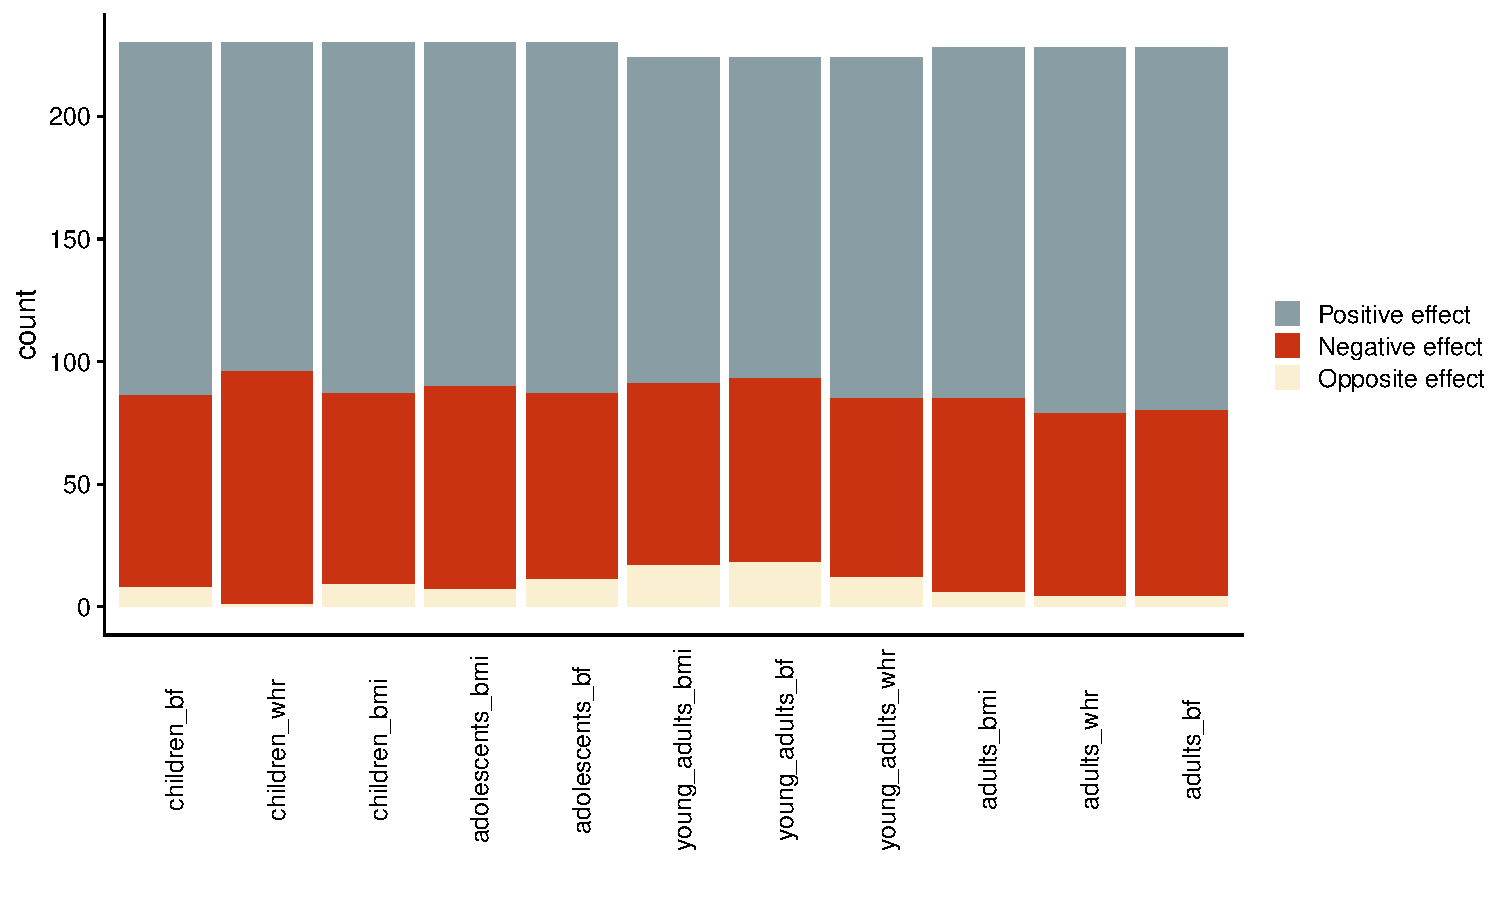
\includegraphics[width=1\linewidth]{data/observational/figures/plot_directional_consistency_across_models_within_exposures_groups} \caption[Directional consistency between effect estimates across three linear models within exposures and age groups]{\textbf{Directional consistency between effect estimates across three linear models within exposures and age groups}. A positive effect reflects all model betas being in the positive direction; a negative effect reflects all model betas being in a negative direction; opposite effect reflects different directions for the model betas. For example, if the association between body mass index (BMI) and metabolite A is positive for model 1, 2, and 3 a positive association will be reported. If all three models show a negative direction of effect between BMI and metabolite A, a negative direction of effect will be reported. If one model shows a direction of effect that is positive and the other models give negative directions of effect, an opposite direction of effect will be reported. WHR = waist hip ratio; BF = body fat percentage.}\label{fig:observational-figure-directional-consistency}
\end{figure}
\hypertarget{directional-consistency-between-effect-estimates-for-linear-model-2-across-exposures-within-age-groups}{%
\subsubsection{Directional consistency between effect estimates for linear model 2 across exposures within age groups}\label{directional-consistency-between-effect-estimates-for-linear-model-2-across-exposures-within-age-groups}}

Given the broad agreement between models, including the high correlation observed for effects between model 2 and model 3 (Spearmans rho = 0.81--0.995; Appendix \ref{appendix-observational-correlations}), and the fact that model 3 was not run for children as data on physical activity were not available, results here on are presented for model 2 (all data are available on \href{https://github.com/mattlee821/000_thesis/tree/master/index/data/observational/results}{GitHub}).

\par

Across the three exposures (BMI, WHR, and BF) within each age group, effects showed mostly consistent directions of effect, the majority of which were positive (i.e., adiposity was associated with an increase in metabolites; Figure \ref{fig:observational-figure-directional-consistency-2}). Where there were the most inconsistent directions across exposures was for children, with 21\% of metabolites showed inconsistent directions of effect. For adolescents, young adults, and adults 5\%, 9\%, and 5\% of metabolites showed inconsistent directions of effect across measures of adiposity, respectively. A large proportion of metabolites with evidence for a consistent direction of effect across all three exposures also reached the multiple testing threshold for all three adiposity measures for model 2: children = 110 out of 230 metabolites, adolescents = 148 out of 230 metabolites, young adults = 164 out of 224 metabolites, and adults = 180 out of 228 metabolites.

\par

Of the 220 metabolites measured across all age groups, directional consistency was supported by strong evidence of correlation across exposures within age groups (Spearmans rho = 0.61--0.97) and, within exposures across age groups (Spearmans rho = 0.48--0.82; Appendix \ref{appendix-observational-correlations}).

\par




\begin{figure}
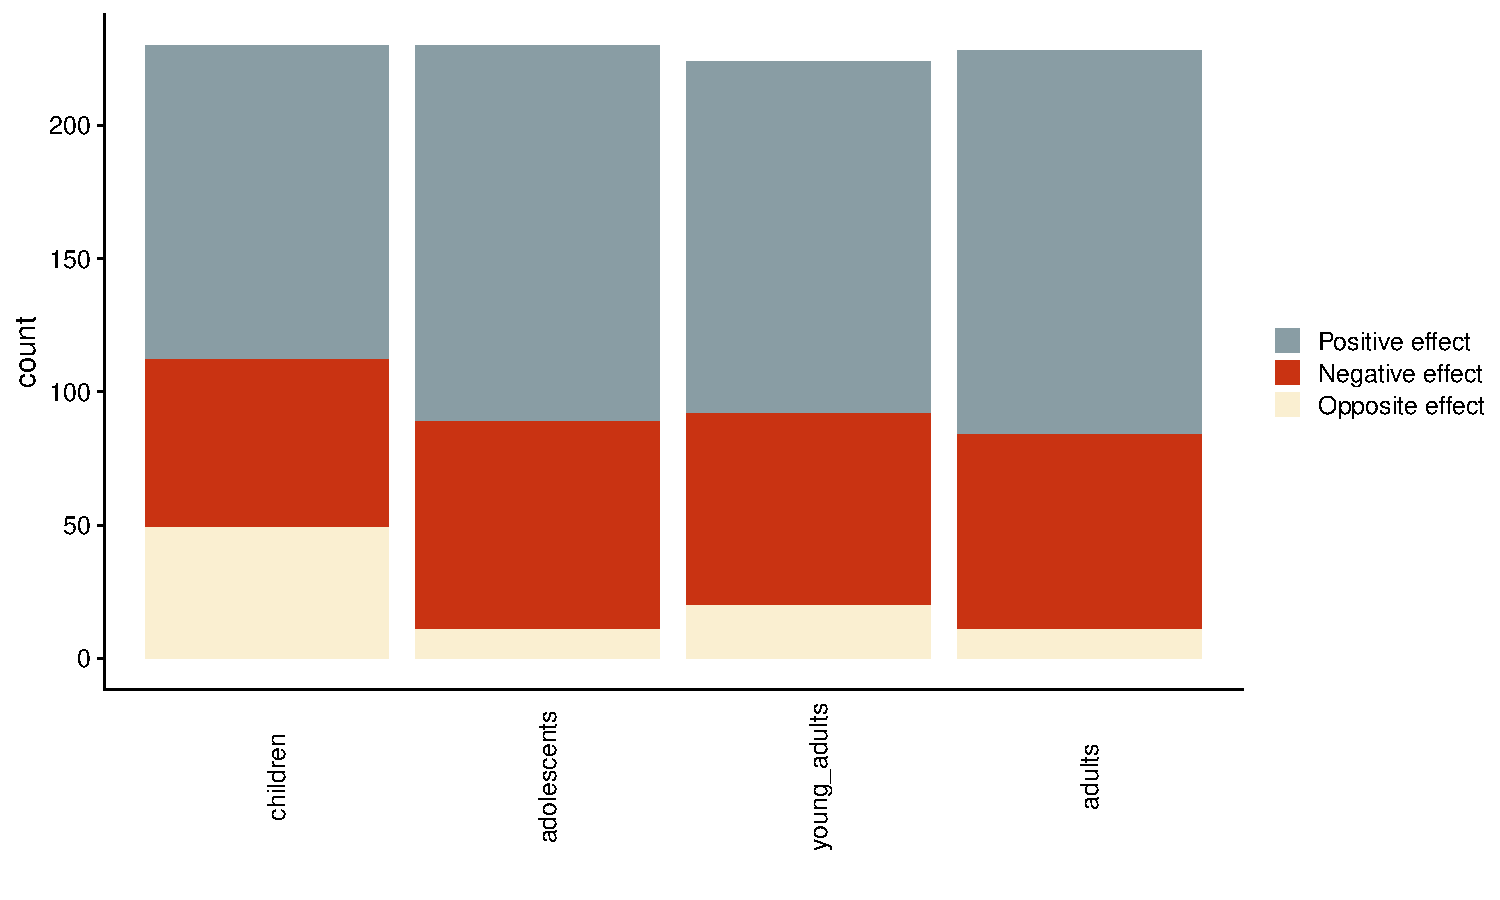
\includegraphics[width=1\linewidth]{data/observational/figures/plot_directional_consistency_model2_within_exposures_groups} \caption[Directional consistency for linear model 2 across exposures within age groups]{\textbf{Directional consistency for linear model 2 across exposures within age groups}. A positive effect reflects all model effect estimates being in the positive direction; a negative effect reflects all model effect estimates being in a negative direction; opposite effect reflects different directions for the model effect estimates. For example, if the association between body mass index (BMI), waist hip ratio, and body fat percentage and metabolite A is positive a positive association will be reported. If all three exposures show a negative direction of effect with metabolite A, a negative direction of effect will be reported. If one exposure shows a direction of effect that is positive and the other exposures give negative directions of effect, an opposite direction of effect will be reported.}\label{fig:observational-figure-directional-consistency-2}
\end{figure}
\hypertarget{global-metabolic-profile}{%
\subsubsection{Global metabolic profile}\label{global-metabolic-profile}}

To aid visual comparison between metabolite subclasses, derived measures were visualised separately to non-derived measures, and are presented in the Appendix (\ref{appendix-observational-figures}). Derived measures are metabolites that are not directly measured by the metabolomic array and are instead derived during the processing of the raw NMR spectra. Derived measures include ratios such as cholesterol esters in very large very low density lipoprotein (VLDL) to total lipids in very large VLDL ratio.

\par

Overall, the global pattern of association was very similar for all measures of adiposity for children (Figure \ref{fig:observational-figure-circosplot-main-children}), adolescents (Figure \ref{fig:observational-figure-circosplot-main-adolescents}), young adults (Figure \ref{fig:observational-figure-circosplot-main-young-adults}), and adults (Figure \ref{fig:observational-figure-circosplot-main-adults}) across all directly measured metabolites (larger figures are available on GitHub, for \href{https://github.com/mattlee821/000_thesis/blob/master/index/data/observational/figures/circosplot_metabolites_children.pdf}{children}, \href{https://github.com/mattlee821/000_thesis/blob/master/index/data/observational/figures/circosplot_metabolites_adolescents.pdf}{adolescents}, \href{https://github.com/mattlee821/000_thesis/blob/master/index/data/observational/figures/circosplot_metabolites_young_adults.pdf}{young adults}, and \href{https://github.com/mattlee821/000_thesis/blob/master/index/data/observational/figures/circosplot_metabolites_adults.pdf}{adults}). Across all age groups, the largest effect sizes for directly measured metabolites were found for the fatty acids subclass; the total fatty acids metabolite showed the largest effect size across all exposures for each age group. Metabolites in small VLDL, medium VLDL, large VLDL, and very large VLDL subclasses were the only metabolites to reach the specified multiple testing thresholds across all exposures and age groups. On the whole, effect sizes were lowest in children and increased with age. The largest effect sizes in adults, total fatty acids (change in metabolite (mmol/l) per SD change in the exposure = 0.51), was twice that observed in children (change in metabolite (mmol/l) per SD change in the exposure = 0.21).

\par

For derived measures, the global pattern of association was very similar within age groups across exposures and across age groups within exposures (Appendix \ref{appendix-observational-figures}). There was considerable variation within subclasses for derived measures. For adults (Figure \ref{appendix-observational-figure-circos-adults}), unlike the other age groups, extreme effect sizes were found for a number of metabolites (summary of effect size across all exposures and derived metabolites: minimum = -1.18 x 10\textsuperscript{-15}; median = -0.11; mean = -2.09 x 10\textsuperscript{-13}; maximum = 1.95 x 10\textsuperscript{11}). The majority of effect sizes observed for adults were around the median value.

\par




\begin{figure}
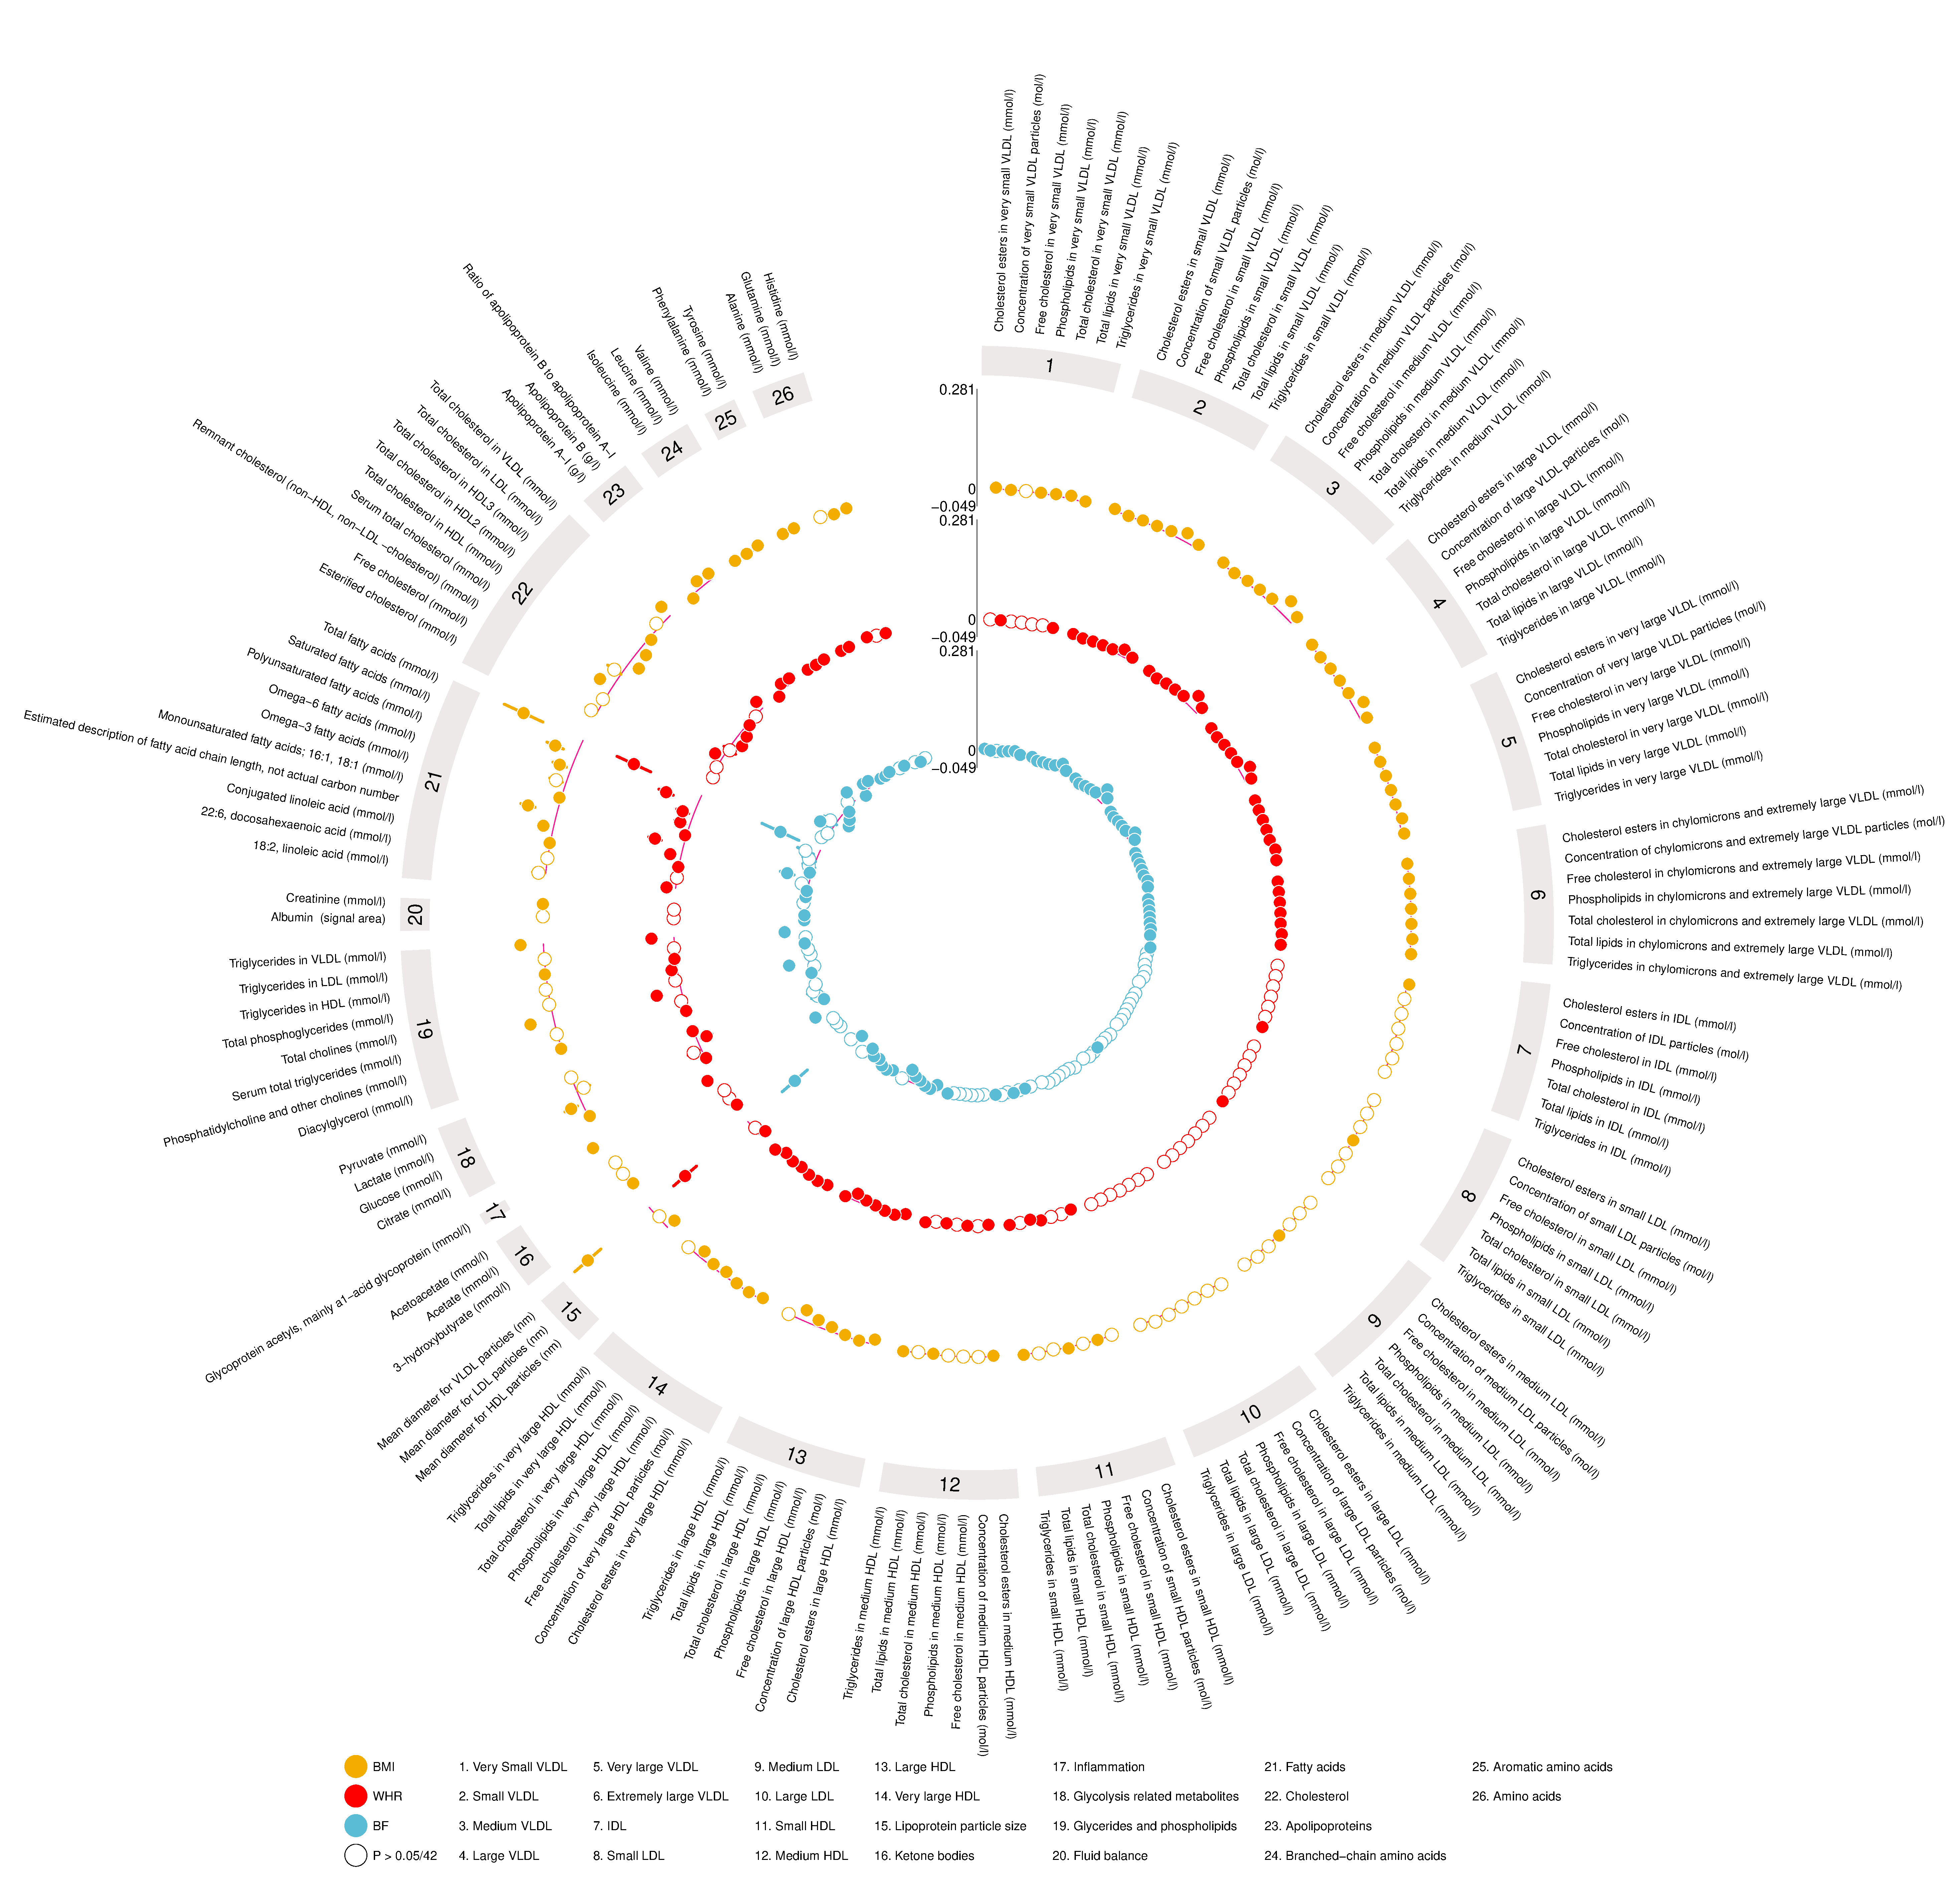
\includegraphics[width=1\linewidth]{data/observational/figures/circosplot_metabolites_children} \caption[Effect estimates from linear regression of adiposity measures on metabolites in children]{\textbf{Effect estimates from linear regression of adiposity measures on metabolites in children}. The Circos plot shows each track as one of the measures of adiposity; the outer track is body mass index (BMI), the middle track is waist hip ratio (WHR), the inner track is body fat percentage (BF). Effect estimates are given as a change in the raw metabolite unit per standard deviation change in the exposure; 95\% confidence intervals are shown and may be hidden by the point estimate if very tight. Solid points indicate a multiple testing threshold has been reached (0.05/42). Available on \href{https://github.com/mattlee821/000_thesis/blob/master/index/data/observational/figures/circosplot_metabolites_children.pdf}{GitHub}. Circos plot of derived measures also available on \href{https://github.com/mattlee821/000_thesis/blob/master/index/data/observational/figures/circosplot_derived_metabolites_children.pdf}{GitHub}.}\label{fig:observational-figure-circosplot-main-children}
\end{figure}
\newpage




\begin{figure}
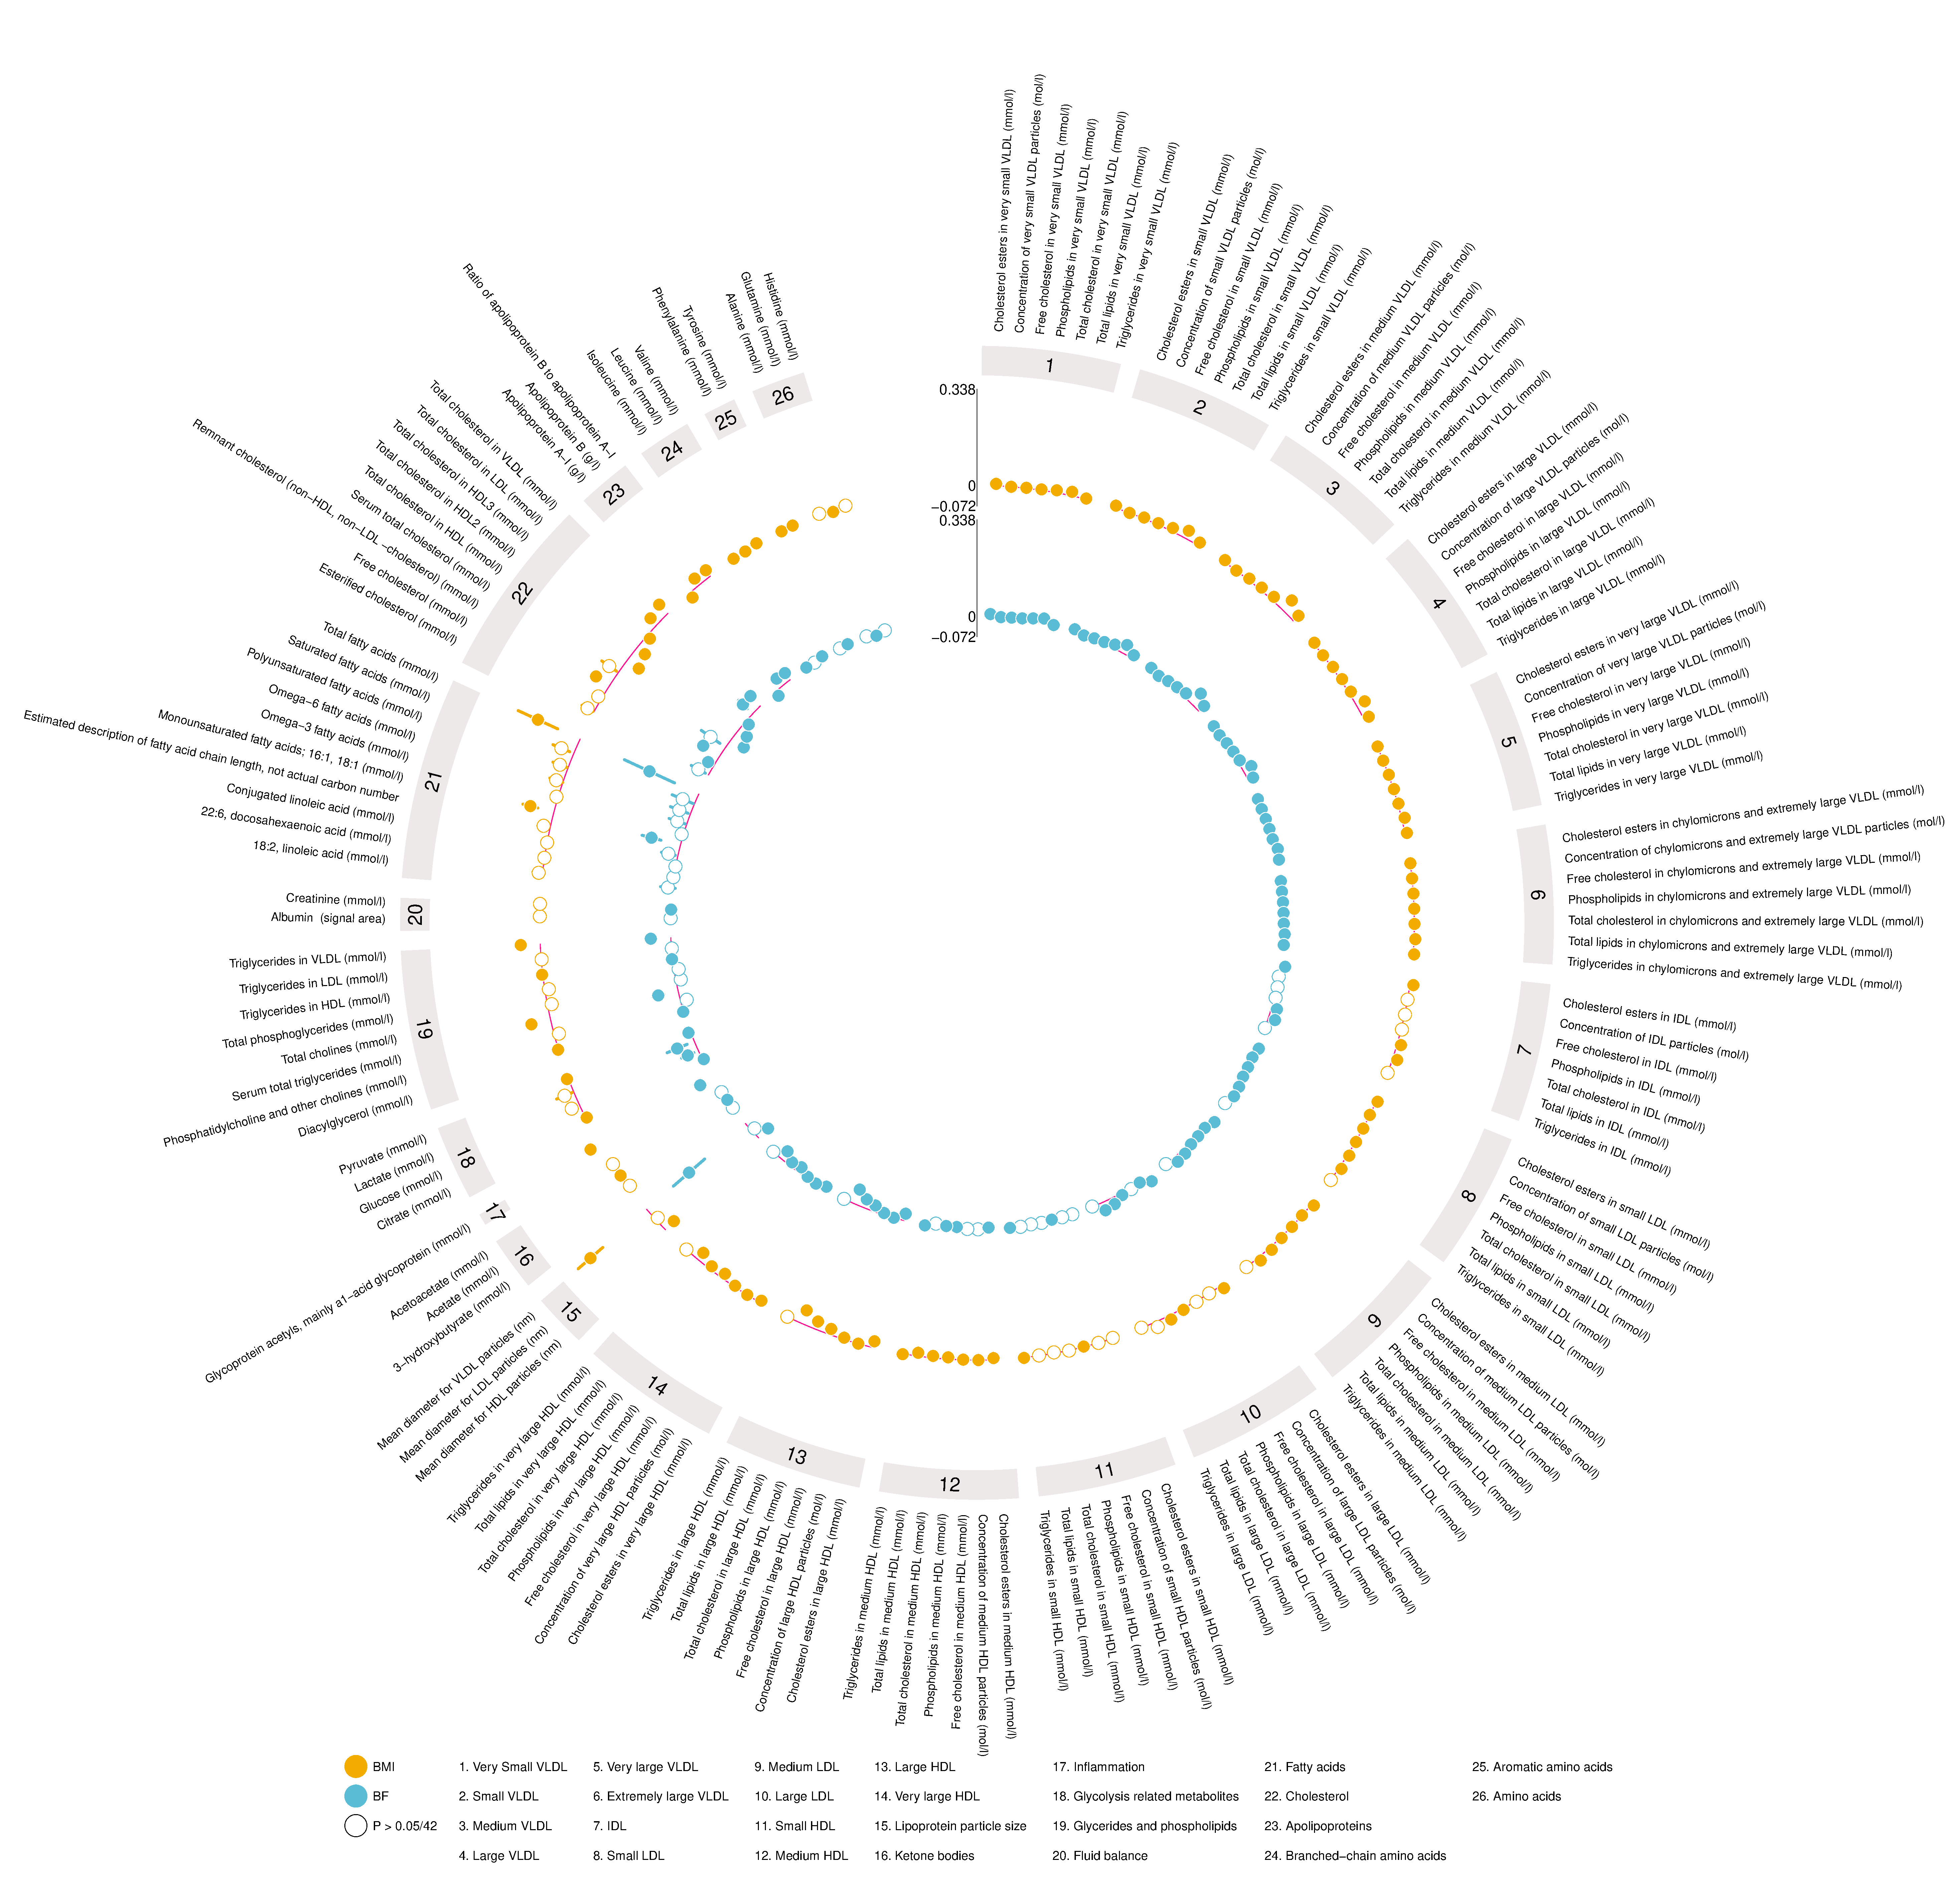
\includegraphics[width=1\linewidth]{data/observational/figures/circosplot_metabolites_adolescents} \caption[Effect estimates from linear regression of adiposity measures on metabolites in adolescents]{\textbf{Effect estimates from linear regression of adiposity measures on metabolites in adolescents}. The Circos plot shows each track as one of the measures of adiposity; the outer track is body mass index (BMI), the inner track is body fat percentage (BF). Effect estimates are given as a change in the raw metabolite unit per standard deviation change in the exposure; 95\% confidence intervals are shown and may be hidden by the point estimate if very tight. Solid points indicate a multiple testing threshold has been reached (0.05/42). Available on \href{https://github.com/mattlee821/000_thesis/blob/master/index/data/observational/figures/circosplot_metabolites_adolescents.pdf}{GitHub}. Circos plot of derived measures also available on \href{https://github.com/mattlee821/000_thesis/blob/master/index/data/observational/figures/circosplot_derived_metabolites_adolescents.pdf}{GitHub}.}\label{fig:observational-figure-circosplot-main-adolescents}
\end{figure}
\newpage




\begin{figure}
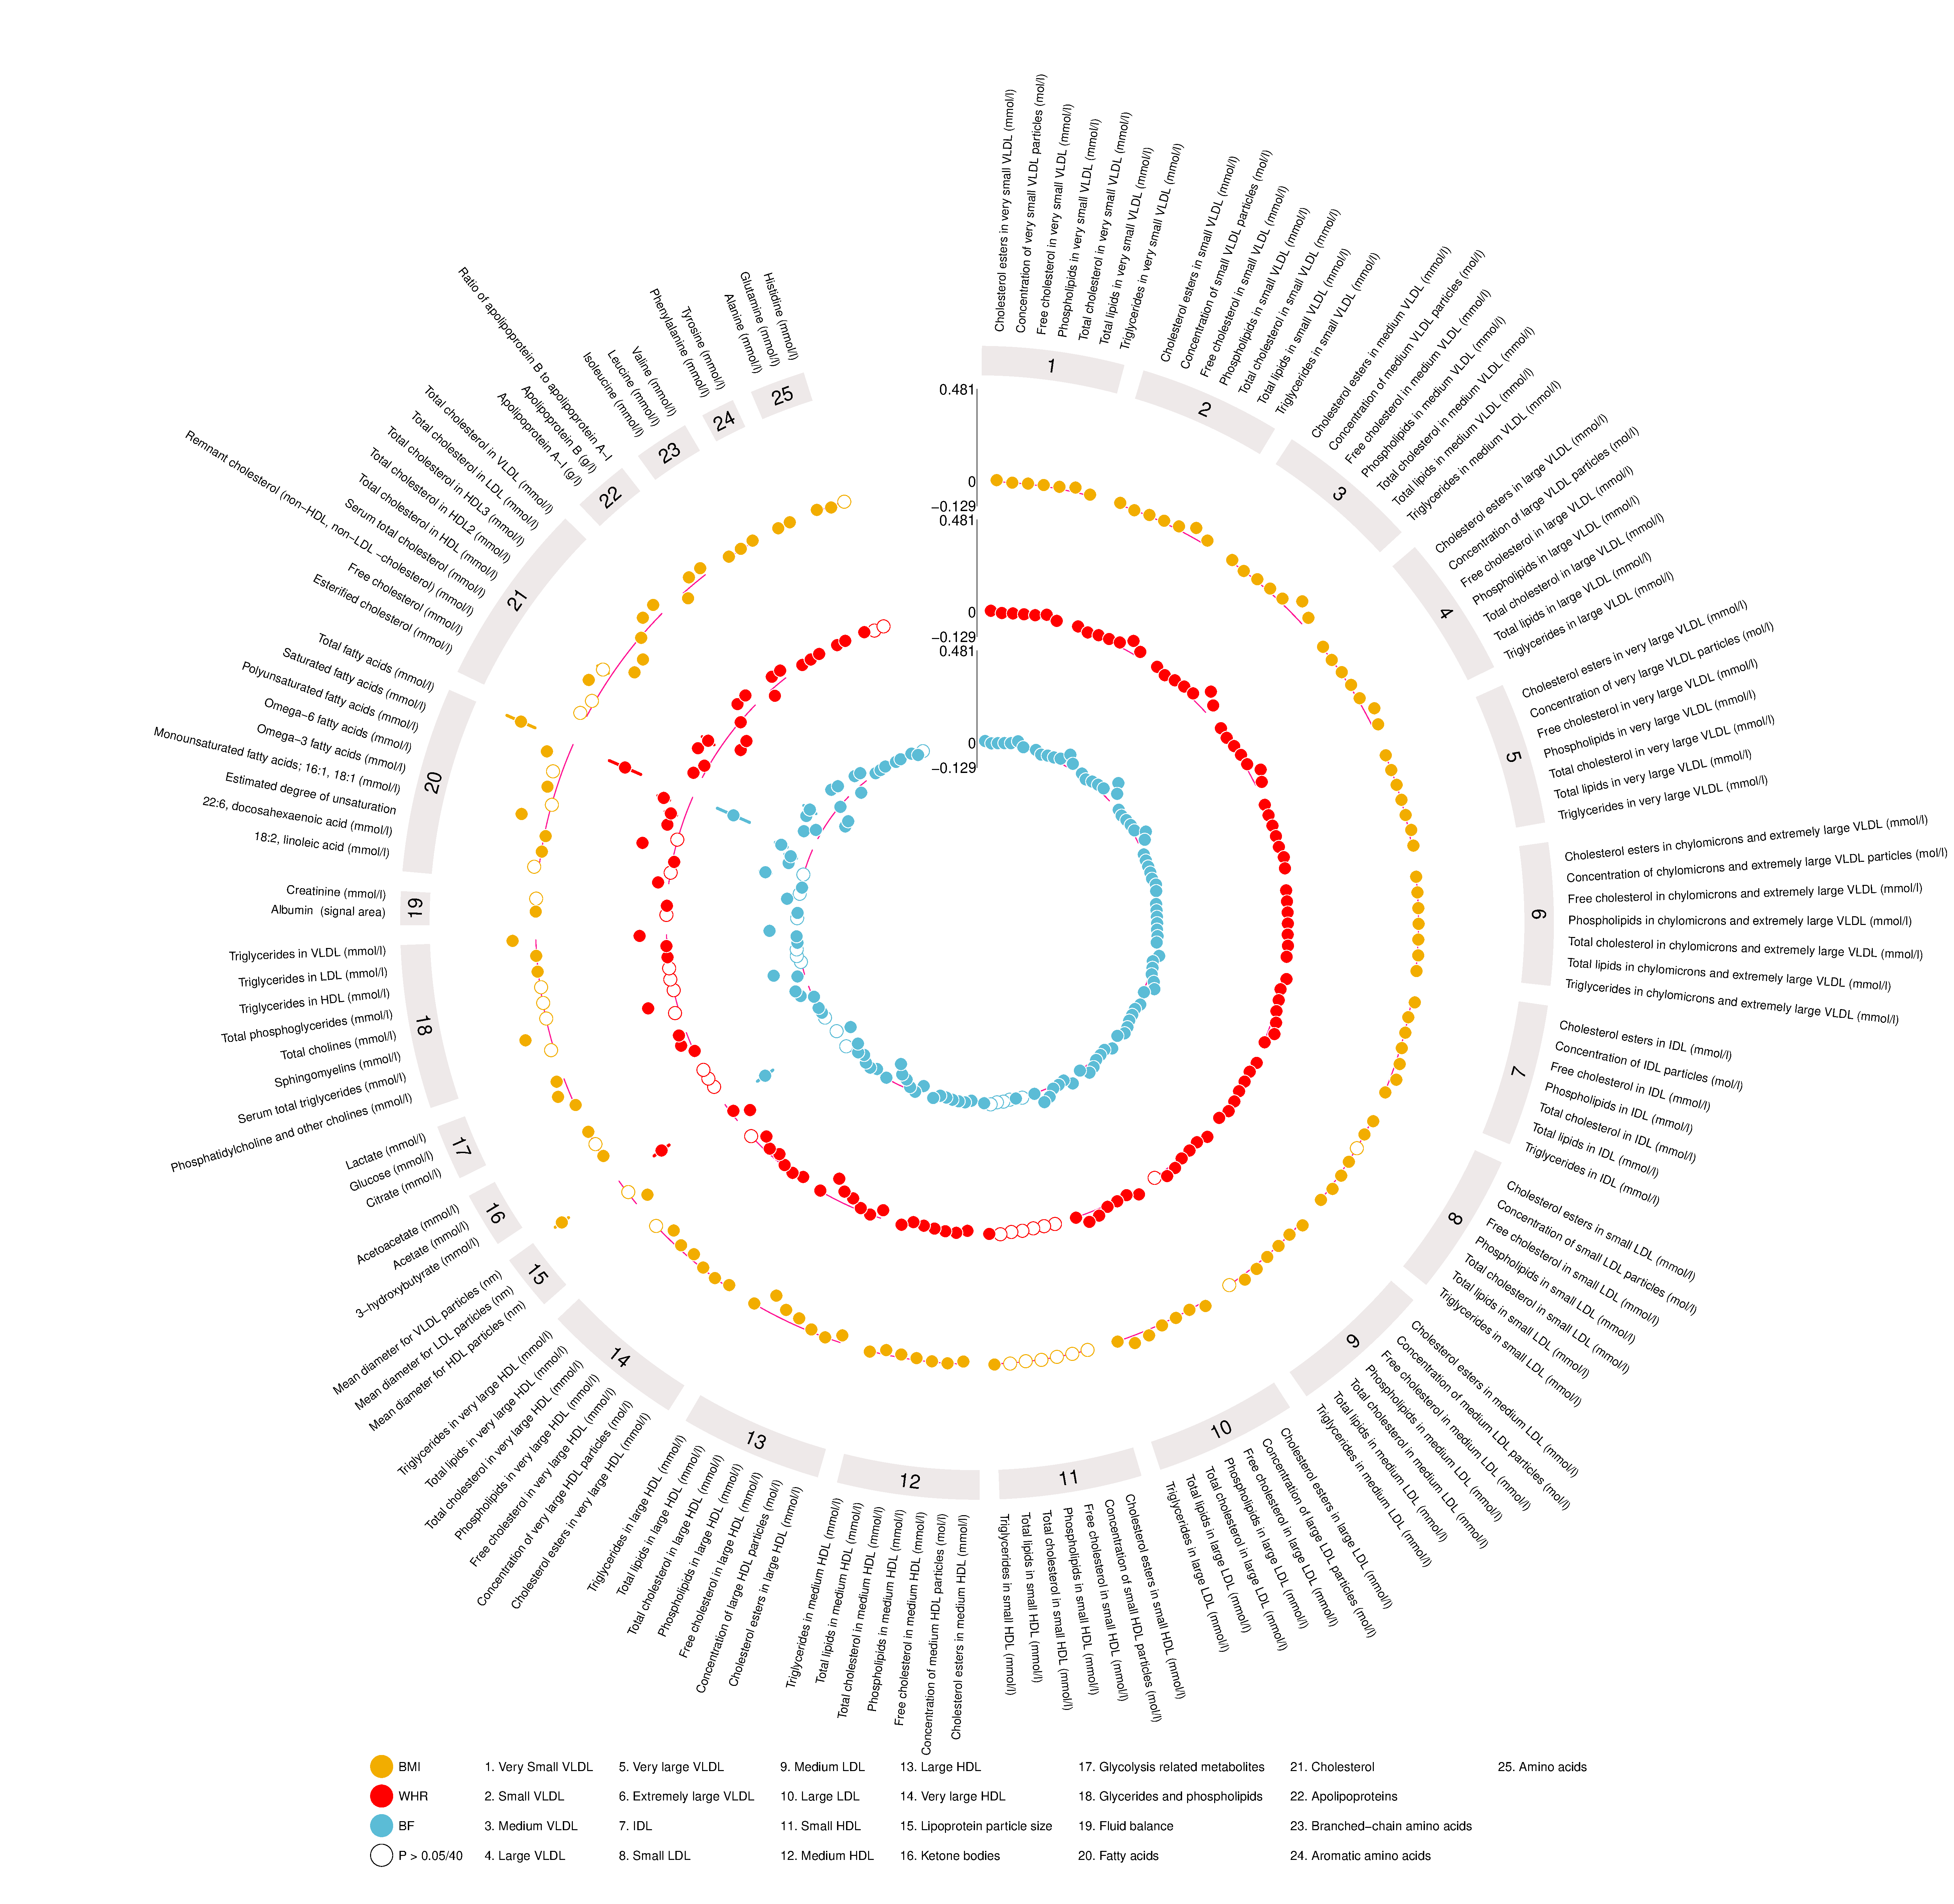
\includegraphics[width=1\linewidth]{data/observational/figures/circosplot_metabolites_young_adults} \caption[Effect estimates from linear regression of adiposity measures on metabolites in young adults]{\textbf{Effect estimates from linear regression of adiposity measures on metabolites in young adults}. The Circos plot shows each track as one of the measures of adiposity; the outer track is body mass index (BMI), the middle track is waist hip ratio (WHR), the inner track is body fat percentage (BF). Effect estimates are given as a change in the raw metabolite unit per standard deviation change in the exposure; 95\% confidence intervals are shown and may be hidden by the point estimate if very tight. Solid points indicate a multiple testing threshold has been reached (0.05/40). Available on \href{https://github.com/mattlee821/000_thesis/blob/master/index/data/observational/figures/circosplot_metabolites_young_adults.pdf}{GitHub}. Circos plot of derived measures also available on \href{https://github.com/mattlee821/000_thesis/blob/master/index/data/observational/figures/circosplot_derived_metabolites_young_adults.pdf}{GitHub}.}\label{fig:observational-figure-circosplot-main-young-adults}
\end{figure}
\newpage




\begin{figure}
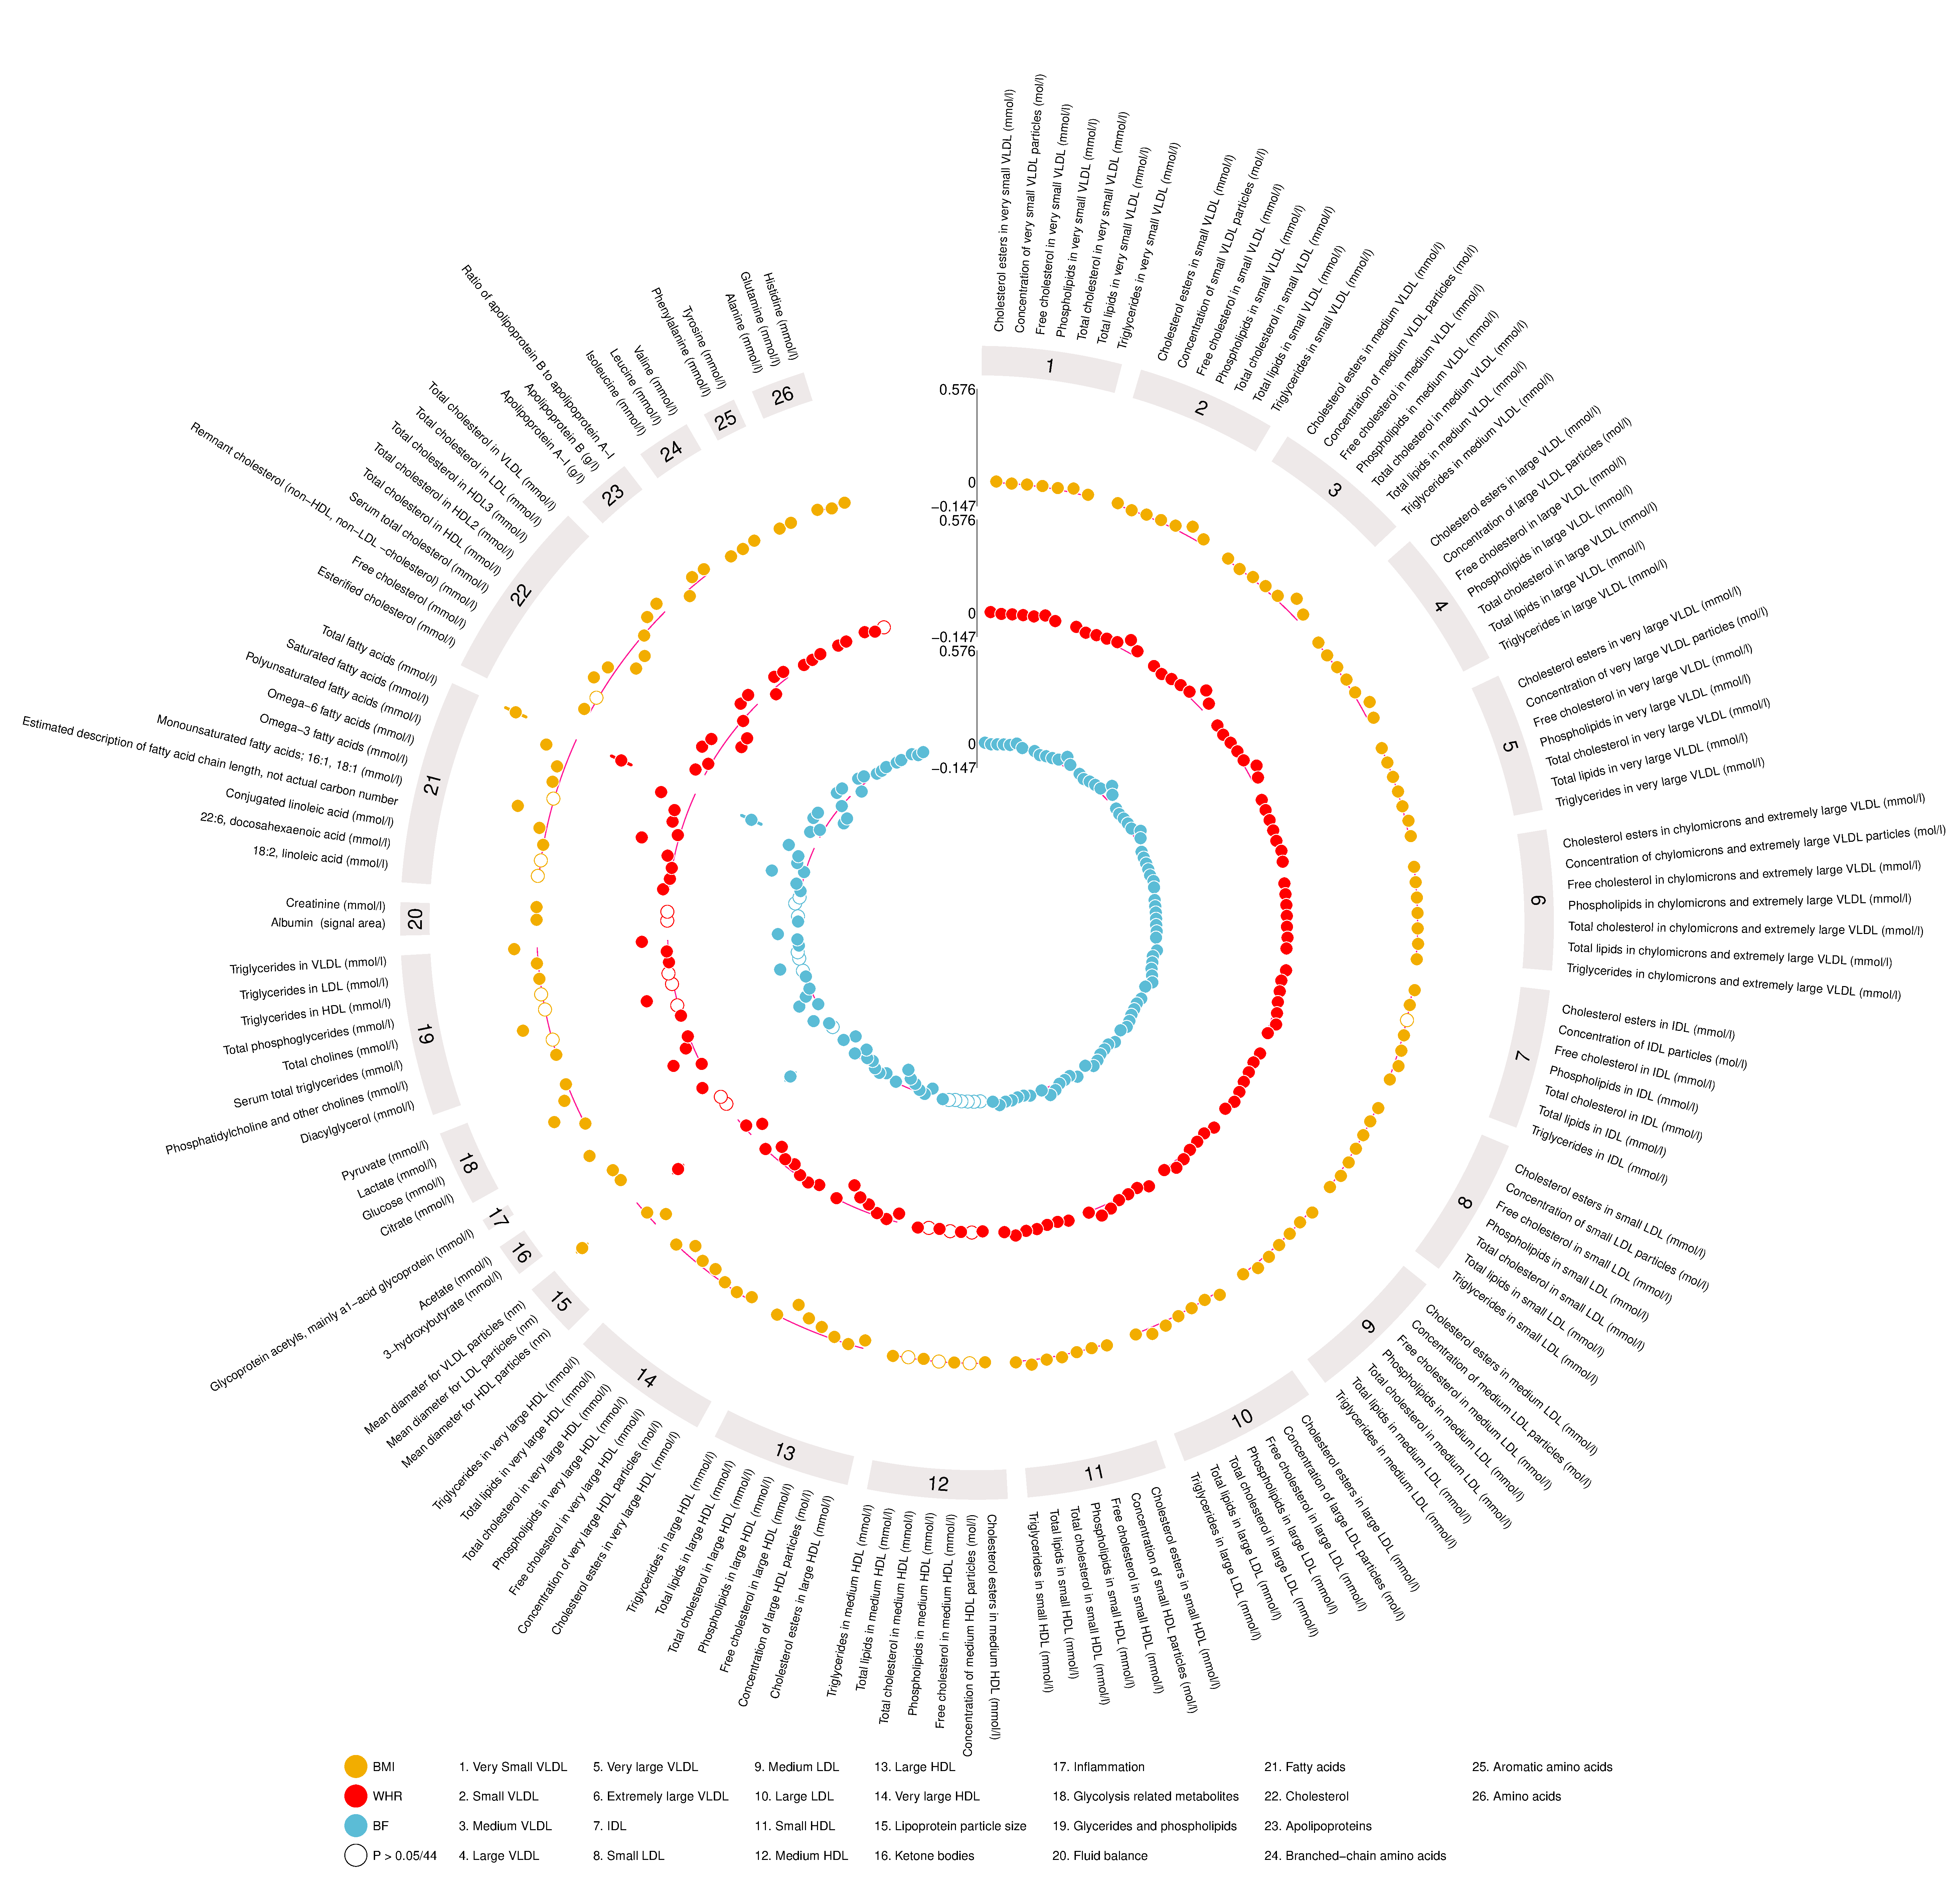
\includegraphics[width=1\linewidth]{data/observational/figures/circosplot_metabolites_adults} \caption[Effect estimates from linear regression of adiposity measures on metabolites in adults]{\textbf{Effect estimates from linear regression of adiposity measures on metabolites in adults}. The Circos plot shows each track as one of the measures of adiposity; the outer track is body mass index (BMI), the middle track is waist hip ratio (WHR), the inner track is body fat percentage (BF). Effect estimates are given as a change in the raw metabolite unit per standard deviation change in the exposure; 95\% confidence intervals are shown and may be hidden by the point estimate if very tight. Solid points indicate a multiple testing threshold has been reached (0.05/44). Available on \href{https://github.com/mattlee821/000_thesis/blob/master/index/data/observational/figures/circosplot_metabolites_adults.pdf}{GitHub}. Circos plot of derived measures also available on \href{https://github.com/mattlee821/000_thesis/blob/master/index/data/observational/figures/circosplot_derived_metabolites_adults.pdf}{GitHub}.}\label{fig:observational-figure-circosplot-main-adults}
\end{figure}
\newpage

\hypertarget{subclass-results}{%
\subsubsection{Subclass results}\label{subclass-results}}

When looking at directly measured metabolite subclasses, there were associations between measures of adiposity and all subclasses except for large low density lipoprotein (LDL) in children, where CIs for all large LDL metabolites crossed the null. For the derived measure subclasses, associations were observed across measures of adiposity for all subclasses except extremely large VLDL ratios in young adults and adults.

\par

Across all age groups and exposures, associations with every metabolite in a particular subclass was observed for small VLDL, medium VLDL, large VLDL, very large VLDL, and extremely large VLDL. As age increased, the number of associations within subclasses tended to increase across all measures of adiposity. For example, across small LDL, medium LDL, and large LDL, few associations were observed across measures of adiposity in children, however, in adolescents and young adults, a majority of metabolites showed evidence of association; while in adults, all metabolites showed evidence of association. Effect sizes tended to increase with age as well, for example, the largest effects seen for small, medium, and large LDL metabolites were in adults and young adults (Figure \ref{fig:observational-figure-forestplot-subclass-LDL}).

\par




\begin{figure}
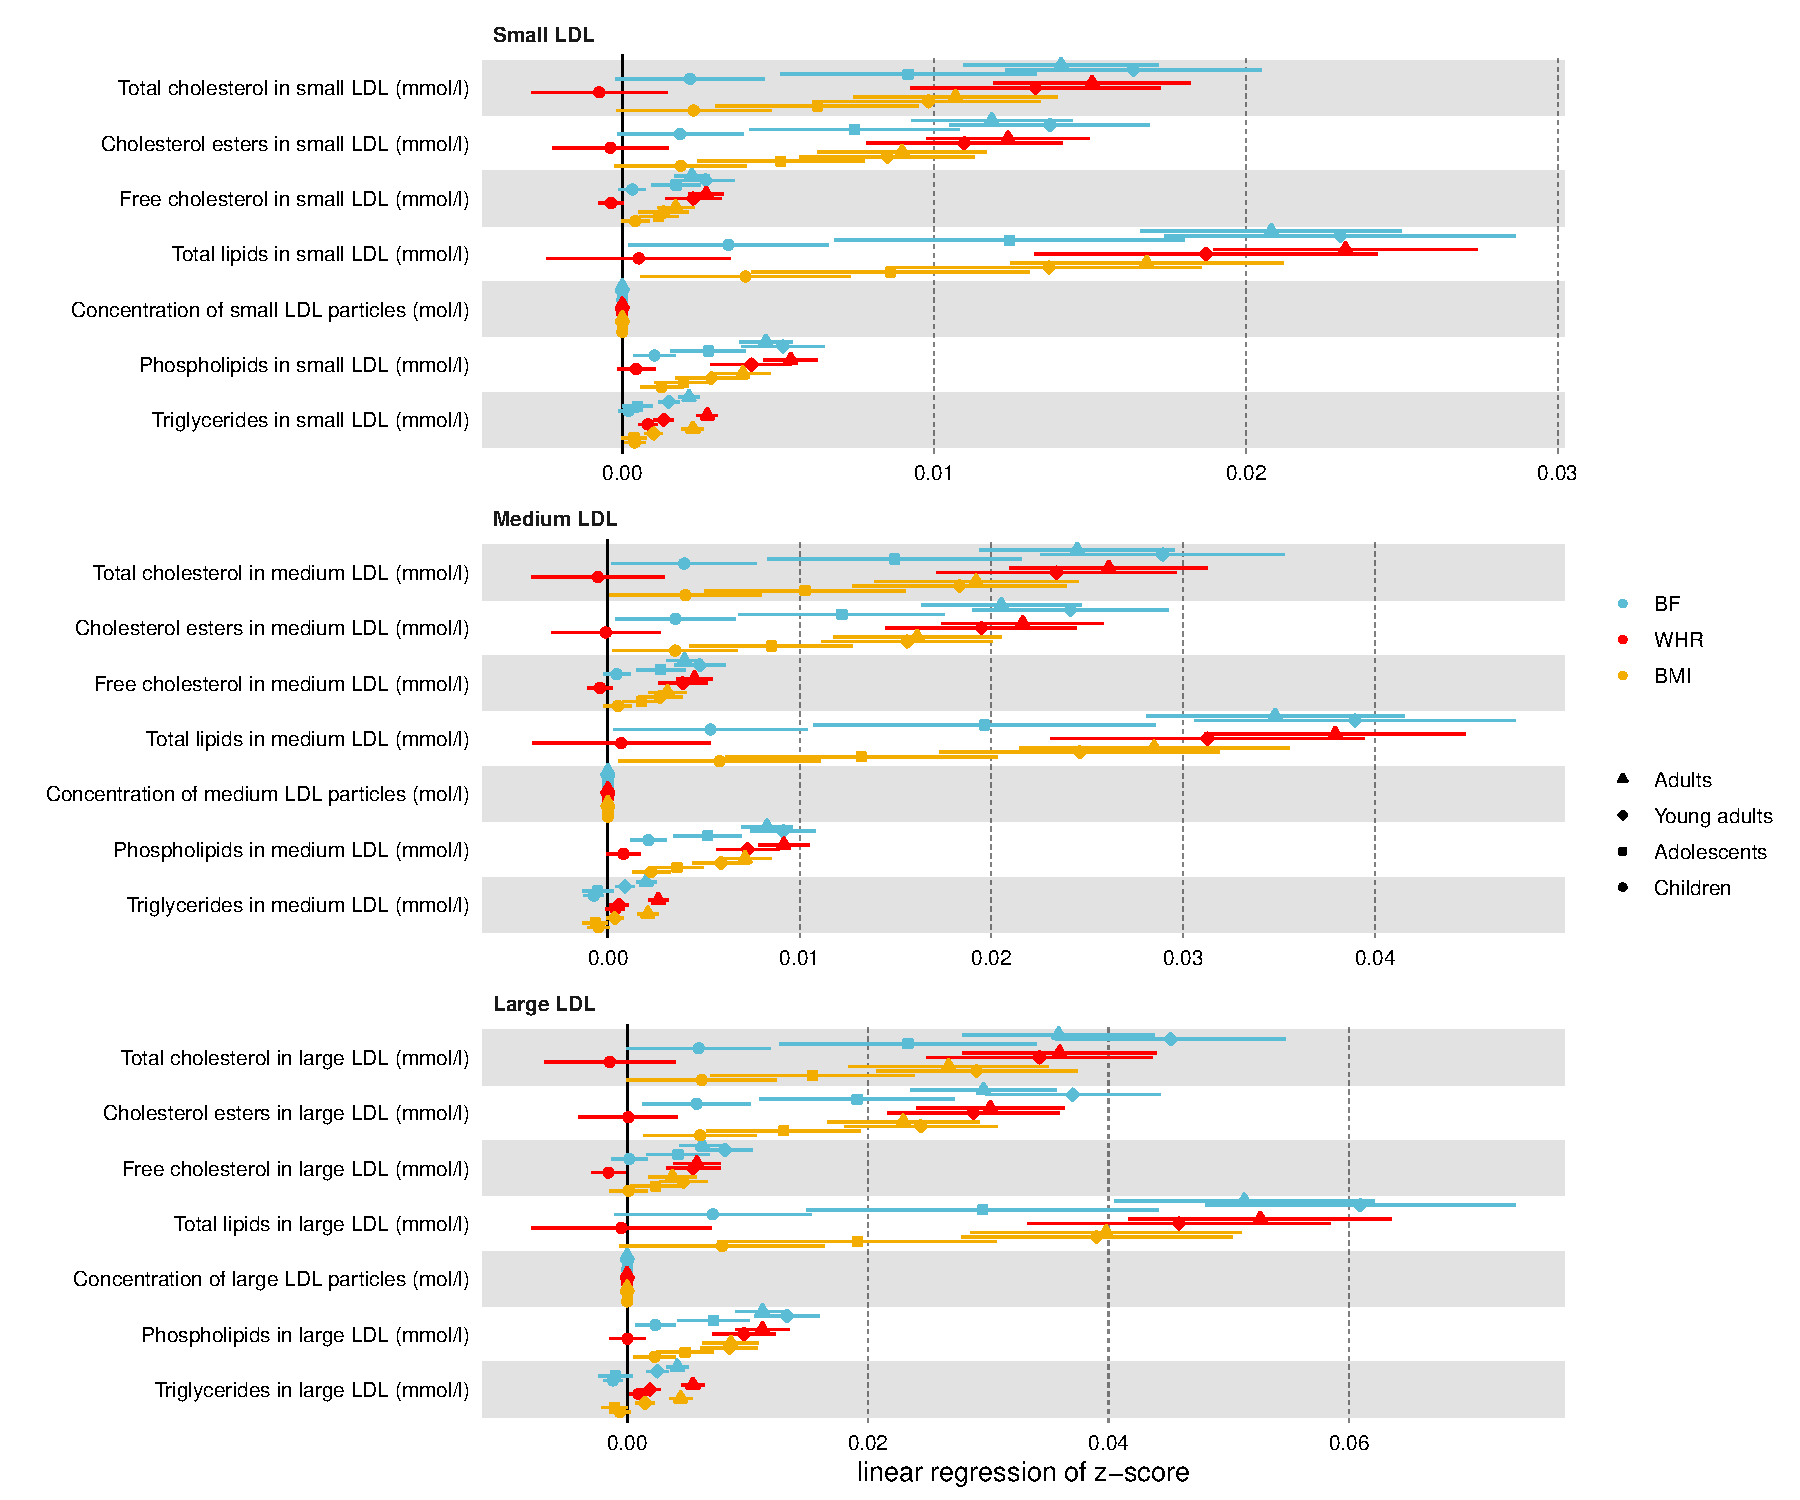
\includegraphics[width=1\linewidth]{data/observational/figures/forestplot_subclass_LDL} \caption[Effect estimates from linear regression using model 2 of adiposity measures on metabolites in all age groups for small, medium, and large LDL subclasses]{\textbf{Effect estimates from linear regression using model 2 of adiposity measures on metabolites in all age groups for small, medium, and large LDL subclasses}. Effect estimates are given as a change in the raw metabolite unit per standard deviation change in the exposure. 95\% confidence intervals are shown. BMI = body mass index; WHR = waist hip ratio; BF = body fat percentage. Available on \href{https://github.com/mattlee821/000_thesis/blob/master/index/data/observational/figures/forestplot_subclass_LDL.pdf}{GitHub}.}\label{fig:observational-figure-forestplot-subclass-LDL}
\end{figure}
To summarise the results for directly measured metabolites from model 2 across exposures and across age groups, the largest mean positive effect estimate was observed for metabolites in the lipoprotein particle size, fatty acids, and inflammation subclasses. The largest mean negative effect estimate was observed for metabolites in the medium, large, and very large HDL, and ketone bodies subclasses. The largest median effect estimates however were observed for the fatty acids, inflammation, and cholesterol subclasses, while the largest negative median effect estimates were observed for medium, large, and very large HDL, and ketone bodies and lipoprotein particle size subclasses. A summary (minimum, maximum, mean, and median values) for each age group across subclasses for model 2 are available on \href{https://github.com/mattlee821/000_thesis/tree/master/index/data/observational/tables/effect_size_summary}{GitHub}.

\par

The above summary does not take account of the variation within subclasses. That is, metabolites within a subclass do not all have the same direction of effect. Focussing on results for adults given the directional consistency observed across age groups, all metabolites in the very small, small, medium, large, very large, and extremely large VLDL, and IDL, small, medium, and large LDL, and small HDL, fatty acids, inflammation, and branched-chain and aromatic amino acids subclasses had positive directions of effect (Figure on \href{https://github.com/mattlee821/000_thesis/blob/master/index/data/observational/figures/adults_model2_effect_summary.pdf}{GitHub}). A majority of metabolites within the cholesterol, apolipoproteins, glycolysis related metabolites, and glycerides and phospholipids subclasses had positive directions of effect. All metabolites within the ketone bodies, and large and very large HDL subclasses had negative directions of effect. A majority of metabolites within the medium HDL, lipoprotein particle size, and amino acids subclasses had negative directions of effect.

\par

Directions of effect were broadly consistent across exposures. The exceptions were for the negative effect of BMI on phosphatidylcholine and other cholines (change in metabolite (mmol/l) per SD increase in BMI = -0.0024; 95\% CI = -0.014 -- 0.0089; p-value = 0.0057) compared to the positive effects of WHR and BF (neither of which reached the multiple testing threshold), and the positive effect of BF on concentration of medium HDL particles (change in metabolite (mmol/l) per SD increase in BF = 9.81 x 10\textsuperscript{-9}; 95\% CI = 1.73 x 10\textsuperscript{-10} -- 1.95 x 10\textsuperscript{8}; p-value = 0.046), phospholipids in medium HDL (change in metabolite (mmol/l) per SD increase in BF = 0.0015; 95\% CI = -0.0007 -- 0.00379; p-value = 0.19), and total lipids in medium HDL (change in metabolite (mmol/l) per SD increase in BF = 0.0023; 95\% CI = -0.0025 -- 0.0073; p-value = 0.35) compared to the negative effects of BMI and WHR (neither of which reached the multiple testing threshold).

\par

The apolipoproteins apolipoprotein A-1 and apolipoprotein B are markers of LDL and HDL particles respectively. There was a positive association between all three adiposity measures and apolipoprotein A-1, all of which reached the multiple testing threshold (e.g., change in metabolite (g/l) per SD increase in BMI = -0.034; 95\% CI = -0.04 -- -0.03; p-value = 3.64 x 10\textsuperscript{-34}). There was also a negative association between all three adiposity measures and apolipoprotein B all of which reached the multiple testing threshold (e.g., change in metabolite (g/l) per SD increase in BMI = 0.046; 95\% CI = 0.039 -- 0.052; p-value = 2.93 x 10\textsuperscript{-44}). In addition, there was a positive association across all adiposity measures with the ratio of apolipoprotein B to apolipoprotein A-1, all of which reached the multiple testing threshold (e.g., change in ratio of apolipoprotein B to apolipoprotein A-1 per SD increase in BMI = 0.037; 95\% CI = 0.035 -- 0.043; p-value = 2.43 x 10\textsuperscript{-78}).

\par

\hypertarget{Chapter4-wurtz-comparison}{%
\subsection{Comparison with previous work}\label{Chapter4-wurtz-comparison}}

A total of 82 metabolites were measured using the same platform by Wurtz et al.~(2014)\textsuperscript{\protect\hyperlink{ref-Wurtz2014}{286}}. Of these, 42 were also measured across children, adolescents, young adults, and adults in this analysis using ALSAPC. As Wurtz et al., transformed metabolite values into SD units, which was not the case here, directional consistency was investigated with results for model 2. Across all analyses conducted here for model 2, a majority of metabolites showed a consistent direction of effect with the study by Wurtz et al.\textsuperscript{\protect\hyperlink{ref-Wurtz2014}{286}} (Figure \ref{fig:observational-figure-wurtz-comparison}). However, there were some metabolites where the effects from Wurtz et al., were opposite to the effects found here, such as fatty acid chain length and albumin.

\par

The majority of effect estimates were in the positive direction, i.e.~an increase in adiposity was associated with an increase in metabolites. Broadly, adiposity had an increasing effect on 30 metabolites and a decreasing effect on 12 metabolites, i.e.~more than half of effect estimates across all exposures and age groups for a single metabolite were positive or negative. A total of 18 metabolites were positively associated with adiposity in analyses by Wurtz et al., and those conducted in all age groups and exposures here, this included phenylalanine, tyrosine, and apolipoprotein B. Seven metabolites were negatively associated with adiposity across analyses by Wurtz et al., and those conducted in all age groups and exposures here, including citrate and apolipoprotein A-1. Looking at the overall effects for each subclass, there were primarily positive effects of adiposity for subclasses aromatic and branched chain amino acids, cholesterol, fatty acids, glycerides and phospholipids, and glycolysis related metabolites. Primarily negative effects were found for lipoprotein particle size and fatty acids ratios. The remaining subclasses were evenly split between positive and negative associations between adiposity measures and metabolites across analyses (amino acids and fluid balance) or were composed of one metabolite (intermediate density lipoprotein (IDL), inflammation, and ketone bodies). In the latter case, total cholesterol in IDL (IDL) and glycoprotein acetlys (inflammation) were primarily positively associated with adiposity, while acetate (ketone bodies) was primarily negatively associated with adiposity.

\par

\newpage
\thispagestyle{empty}




\begin{figure}

{\centering 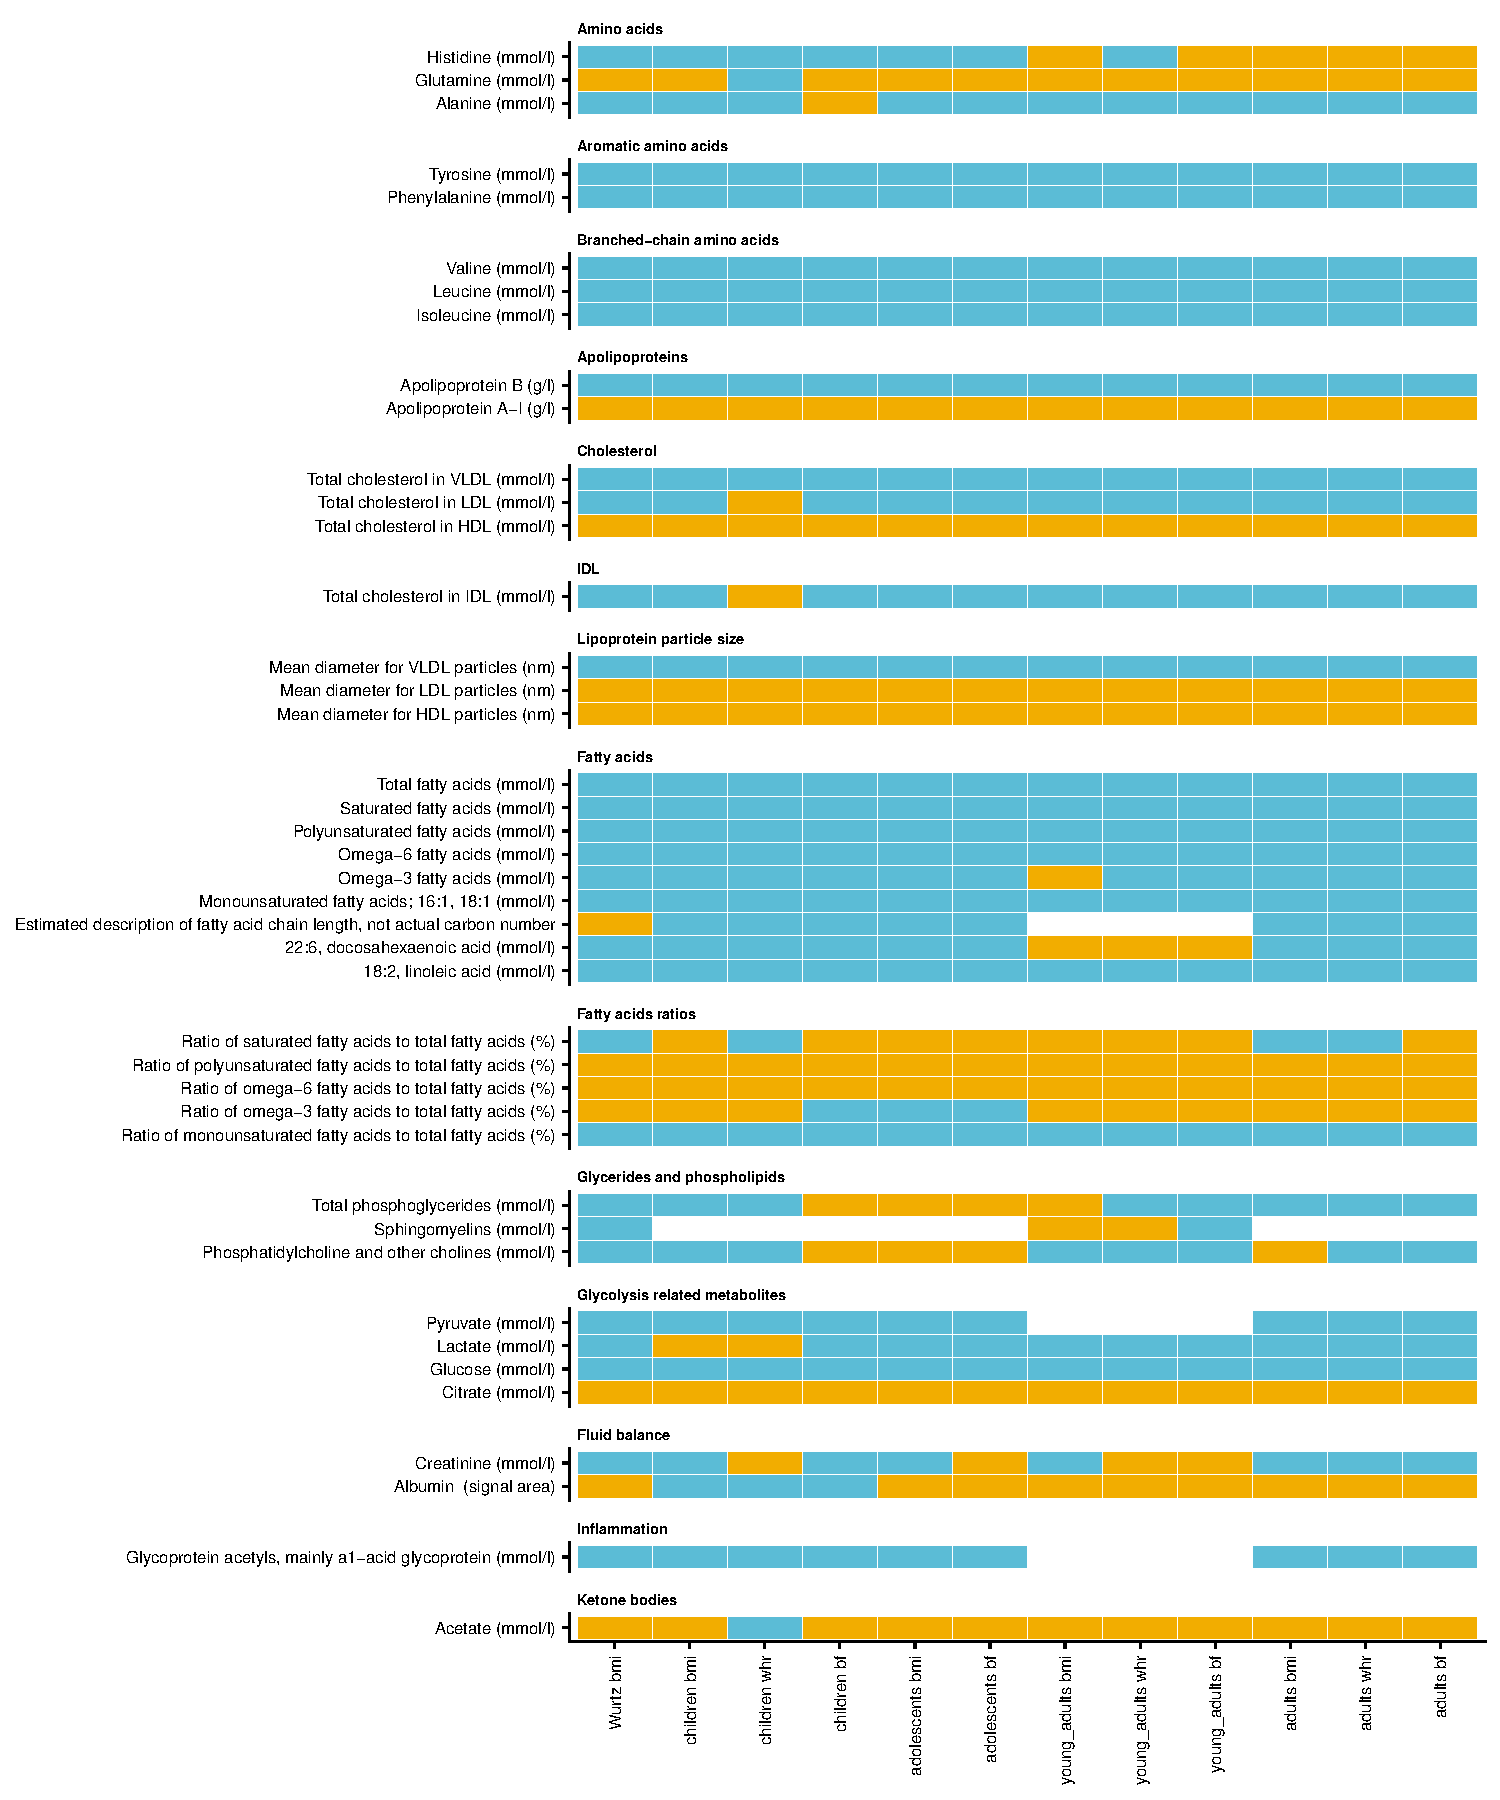
\includegraphics[width=1\linewidth]{data/observational/figures/wurtz_comparison} 

}

\caption[Comparison of the directions of effect estimates from linear regression of adiposity measures on metabolites across all age groups and analysis by Wurtz et al.~(2014)\textsuperscript{\protect\hyperlink{ref-Wurtz2014}{286}}]{\textbf{Comparison of the directions of effect estimates from linear regression of adiposity measures on metabolites across all age groups and analysis by Wurtz et al.~(2014)\textsuperscript{\protect\hyperlink{ref-Wurtz2014}{286}}.} The tile plot shows the direction of effect estimate for 42 metabolites as positive (blue) or negative (orange). If all analyses show the same direction of effect, then that row will be the same colour, e.g., all analyses showing a negative association between adiposity measures and apolipoprotein A-1 and a positive association between adiposity and apolipoprotein B BMI = body mass index; WHR = waist hip ratio; BF = body fat percentage; IDL = intermediate density lipoproteins. White space indicates no analysis was undertaken due to missing data. Available on \href{https://github.com/mattlee821/000_thesis/blob/master/index/data/observational/figures/wurtz_comparison.pdf}{GitHub}.}\label{fig:observational-figure-wurtz-comparison}
\end{figure}
\hypertarget{observational-discussion}{%
\section{Discussion}\label{observational-discussion}}

The association between adiposity and NMR derived metabolites is global, with effects seen across all subclasses of metabolites. These effects are broadly consistent between metabolites within each subclass. In this Chapter, the influence of adiposity on the metabolic profile is demonstrated in an observational framework. These effects persist, not only when measured at different ages, but also when adjusting for covarialbes such as smoking, physical activity, and diet. Effects are similar across multiple measures of adiposity and to those previously reported\textsuperscript{\protect\hyperlink{ref-Wurtz2014}{286}}.

\par

There were similar associations seen in individuals when looking at each exposure across age groups (e.g., the association between BMI on metabolites in children, adolescents, young adults and adults). As age increased, the number of associations within subclasses tended to increase across all measures of adiposity. Fewer associations were observed in children than in adolescents and young adults. A similar metabolic profile was apparent in adults, though effect sizes appeared slightly larger. These results may reflect (i) an effect of prolonged adiposity exposure, (ii) increased variation in metabolites with age, or (iii) be a result of the different SDs of the adiposity measures at different ages. Given that longitudinal work has shown that BMI tracks over time\textsuperscript{\protect\hyperlink{ref-Singh2008}{526},\protect\hyperlink{ref-Buscot2018}{527}}, there may be a dose-response relationship here whereby adiposity has a compounding effect on metabolites over time. Alternatively, metabolite concentrations have been shown to increase in older populations over time\textsuperscript{\protect\hyperlink{ref-Darst2019}{348}} and there was evidence that metabolite variation tended to increase as age increased. However, it is likely that the larger effect sizes observed as age increased are a result of the similar increase in SD of the adiposity measures with age.

\par

Within each age group, there was directional consistency across the three exposures. Effect sizes across exposures were similar within age groups, with overlapping CIs. Effect estimates for the association of BMI on metabolites was generally larger, across age groups, than effect sizes for WHR or BF. Effects for BF appeared to be closer to, and crossed the null more often than those for BMI and WHR. This may suggest that overall body composition in addition to detrimental deposition, may be driving these effects. That is, the compounding effect of increased overall body mass (primarily through increased fat mass; as estimated by BMI) and the predilection to store this additional mass viscerally (as estimated by WHR), may be more powerful than either of these effects alone on the effect of metabolites.

\par

Results were consistent across models, with effect estimates showing the same direction of association for the majority of tests. Effect sizes were broadly similar in the case of models 1 and 2. Effect sizes in model 3 were smaller compared with models 1 and 2. However, CIs overlapped across the majority of tests even if they crossed the null in some instances for model 3 - model 3 had a smaller sample size than model 1 and 2. Broadly speaking, effect estimates attenuated slightly for model 3 compared with model 1 and 2. There was also high consistency in the directions of effect estimates across models within exposures and age groups. These results suggest there could be some confounding but that this was appropriately accounted for given the included covarialbes. Whether these results represent a true causal effect or are subject to reverse causation or residual confounding however requires further investigation.

\par

Previous work by Wurtz et al.~(2014)\textsuperscript{\protect\hyperlink{ref-Wurtz2014}{286}} identified numerous associations between BMI and metabolites in a large population. Results here show a broadly similar pattern of association with those by Wurtz et al., with the majority of the 42 comparable metabolites showing consistent directions of effect. This includes phenylalanine and tyrosine, both of which are known to be increased by adiposity and age\textsuperscript{\protect\hyperlink{ref-Ho2016}{409},\protect\hyperlink{ref-Newgard2009}{410},\protect\hyperlink{ref-Haufe2016}{528}--\protect\hyperlink{ref-Kim2010}{533}}, as well as consistent negative associations with seven metabolites, including apolipoprotein A-1 which is the major component of HDL particles and enables uptake of lipids by HDL particles and the subsequent recycle and excretion of lipids\textsuperscript{\protect\hyperlink{ref-Feingold2000}{534},\protect\hyperlink{ref-Marz2017}{535}}. Differences in effect estimate direction was minimal and split relatively evenly across age groups. Only one metabolite from the Wurtz et al., study, fatty acid chain length, had a direction of effect (negative) that was inconsistent across all age groups here. However, in follow-up Mendelian randomization analysis by Wurtz et al., BMI was positively associated with fatty acid chain length as was found in results in this Chapter. This difference may be a result of residual confounding in the observational analysis conducted by Wurtz et al., as they did not adjust for all of the covarialbes used in analyses in this Chapter.

\par

Of particular note with the analyses performed here, is the variation observed for metabolite values within age groups. Variation was much larger for derived compared to directly measured metabolites. Pre-analysis processing of the metabolomic data, applied here using \texttt{metaboprep}, involved the exclusion of samples (individuals) and metabolites based on a set of QC criteria. However, no filtering was applied to individual data points. Instead, outlying values are flagged for information. However, differentiating between extreme (but real) biological values, and values that are a result of measurement or technical error, is challenging, especially where you have a large number of metabolites with differing distributions. In addition, care is needed when performing filtering or treatment of outlying data points as this can introduce bias. In analyses here, all raw metabolite values were retained for analysis in the first instance. In adults, effect estimates for a number of derived metabolites (across exposures) were considerably larger than effect estimates for other derived metabolites and effect estimates for derived metabolites in the other age groups. An examination of the original data distributions for these metabolites, showed a number of individuals had metabolite values that appeared to be outliers. In post-hoc sensitivity analysis (data not shown), which aimed to investigate whether these individual values were influencing results presented in this Chapter for those derived metabolites, the raw metabolite values in the top and bottom 1\% of metabolite values were changed to the next closest metabolite value below that 1\% threshold. This Winsorization process was performed for all metabolites across age groups. All analyses were repeated and results were highly consistent for the main analysis and this sensitivity analysis for children, adolescents, and young adults. For adults, results were highly consistent for directly measured metabolites and a majority of derived metabolites. However, results for the metabolites that appeared to be outliers in the main analysis were different in sensitivity analysis, with effect sizes much closer to the null and much tighter CIs. This would suggest that results in the main analysis for those derived metabolites were strongly influenced by the outlying metabolite values for a small number of individuals. Given the difficulty in systematically identifying non-biological values, future work should perform sensitivity analyses such as that described here, to investigate whether outlying data has impacted results. This recommendation, as well as methods to control for outlying data, are being added to \texttt{metaboprep} to aid future work.

\par

\hypertarget{strengths-and-limitations}{%
\subsection{Strengths and limitations}\label{strengths-and-limitations}}

The key strengths of this work are the use of (i) rich and large-scale data resource that is ALSPAC, (ii) BMI, WHR and BF as complimentary adiposity measures to comprehensively examine the association between adiposity and metabolites and (iii) the longitudinal nature of the ALSPAC data allowing for this association to be assessed across the lifecourse. ALSPAC is a prospective cohort study with a general population base and here, analyses were performed on up to 4,450 individuals. The breadth of data measured across multiple generations enabled linear models to be adjusted for covarialbes that have been known to affect adiposity and metabolite concentrations\textsuperscript{\protect\hyperlink{ref-Yu2012}{519},\protect\hyperlink{ref-Brennan2020}{520},\protect\hyperlink{ref-Brennan2020}{520}--\protect\hyperlink{ref-ODonoghue2018}{524}}. These analyses were performed across two generations of individuals, G0 (the original mothers recruited to the study) and G1 (the children from those pregnancies). Data on G1 individuals were available from multiple time points and, in combination with data from G0 individuals, enabled the investigation of the association between adiposity and metabolites across the lifecourse from childhood to adulthood. The use of multiple measures of adiposity, as has been recommended previously\textsuperscript{\protect\hyperlink{ref-WorldHealthOrganisation2008}{94},\protect\hyperlink{ref-Collaboration2009}{99}} but which has not been explored in relation to metabolic effects, may indicate that overall body composition and deposition is more important in metabolic changes than either component alone.

\par

Analyses here used individuals from two generations, G0 (mothers and fathers) and G1 (offspring) individuals. Although G0 and G1 individuals are independent in the sense that the represent two unique sets of individuals, there is familial overlap between them. There is also overlap for the children, adolescents, and young adults age groups, whereby the same individual may be present in all three age groups. As such, any effects specific to a G1 individual may be propagated through all G1 clinics that individual attends. In addition, there may be familial overlap within the G1 age groups given siblings may be included in the metabolomic data collection. The number of siblings in each age group is likely small. However, given the shared genetics and environment these individuals (siblings, parents, and offspring pairs) will have, effects observed in one individual may be seen in their relative, and so results may not be truly independent within the G1 age groups and across the G1 and G0 age groups. Familial overlap is likely to overestimate the effect size as inclusion of non-independent individuals may introduce confounding (e.g., via genetic similarity or other family-level confounding), which is not being satisfactorily adjusted for in analyses. This would tend to bias results away from the null. Future work could remove related individuals prior to analysis. However, where data is limited and exclusions may reduce power, a linear mixed model accounting for non-independence of observations or the inclusion of genetic principal components to account for relatedness among individuals within the linear model could be used.

\par

Observational analyses are limited due to issues of confounding and reverse causation. Prospective studies, such as ALSPAC, are able to provide some temporal separation between the measurement of an exposure and outcome, and thus mitigate the potential effects of reverse causation. However, as data on adiposity measures and metabolites were collected at the same time, reverse causation remains a limitation. It was however possible to account for the potential effects of confounding by adjusting linear models for measured confounders. Although many measured confounders were included across the models, it is likely these analyses will not have fully accounted for confounding, either due to measurement error or unmeasured confounding. For example, adults were asked `do you take part in physical activity (e.g.~running, swimming, dancing, golf, tennis, squash, jogging, and bowls)?', with possible answers of `no', `occasionally (less than monthly)' and `frequently (once a month or more)'. Broad categories such as these are unlikely to capture the full impact of physical activity on adiposity and metabolites given that `frequently' will encompass individuals who exercise once a month as well as every day. In addition, although it was possible to investigate the association between adiposity and metabolites across the life course, it is likely that the measurements used during adolescence and young adulthood may reflect a time where the G1 individuals were going through puberty. Puberty is likely to have an effect on adiposity and covarialbes such as physical activity, as well as the metabolome, and future work should therefore include pubertal timing as a covariable.

\par

There are two key limitations in regards to metabolomic data. The first is that these data are limited in their breadth. Although a relatively large number of metabolites were investigated, they were predominantly lipid-based. This leaves a broad array of metabolites that have not been investigated. As such, the metabolites investigated here are broadly reflective of the lipidome and not a global metabolic profile. The Nightingale NMR platform does however provides many derived measures, such as ratios and number of bonds. However, there was considerable variation in the concentration of these derived measures compared to directly measured metabolites. Given the relationship between adiposity and lipids, it is unsurprising there were a large number of associations identified. There is thus a clear need to expand beyond lipid-based platforms in investigating the effects of adiposity, as the associations presented here are likely not reflective of a global metabolic profile. Mass spectrometry (MS) platforms, such as those used by Metabolon, are a potential next step. Though there have been a number of studies investigating the association between adiposity and MS-derived metabolites\textsuperscript{\protect\hyperlink{ref-Cirulli2019}{287},\protect\hyperlink{ref-Moore2018}{536},\protect\hyperlink{ref-Perng2020}{537}}, these have not used a complimentary assessment of body composition to assess adiposity and have not been able to investigate this relationship across the life-course.

\par

There is no standardised approach, nor a gold standard, for performing metabolomic quality control. Here, pre-analysis processing of metabolomic data, including outlier detection and removal, was performed using the \texttt{metaboprep} \texttt{R} package. The default settings for exclusions based on metabolite missingness (\(\geq\) 20\%), sample missingness (\(\geq\) 20\%), total sum abundance (\(\geq\) 5 SD), and principal components (\(\geq\) 5 SD; PCs) were used. Most samples were removed for having missingness \textgreater{} 20\% compared to total peak area. These thresholds were arbitrarily defined, or taken from other studies, such as 20\% sample missingness which was previously used, and arbitrarily defined, in Lotta et al., (2021)\textsuperscript{\protect\hyperlink{ref-Lotta2021}{338}}. More stringent thresholds (e.g.~\(\geq\) 5\%) may have resulted in additional sample exclusions. Metadata, such as batch and runday, was not available and could not be included in pre-analysis processing, though this is likely more an issue with MS data. \texttt{metaboprep} calculated the number of independent metabolites using a clustering dendrogram and a tree cut height based on a Spearman's Rho of 0.5. This is one of many clustering approaches that could be used. For example, adjusting the tree cut height to any other value would have resulted in a different number of independent metabolites being identified, which subsequently would have impacted on multiple testing thresholds used. In addition, there is no rule as to what clustering method (i.e., linkage) should be used, and all methods would have produced different results. The complete-linkage method used here is potentially more appropriate for metabolite data compared to single-linkage, where it is possible for clusters to be combined due to a single element of each cluster being linked, even though all other elements of the clusters are not\textsuperscript{\protect\hyperlink{ref-Everitt2011}{538}}. Although most metabolites were shared across age groups, differences in the number of independent metabolites were found. There were also differences in the number of clusters and truly independent metabolites. Similarly, inclusion of derived metabolites resulted in differing numbers of independent metabolites. Metabolites did not undergo transformation to standardise their concentrations in order to preserve clinical utility and improve interpretation of results.

\par

Metabolomic data used here were from EDTA stored plasma and serum samples. There is evidence that the manner in which samples are obtained and stored (e.g., using EDTA) can impact the readings from NMR platforms\textsuperscript{\protect\hyperlink{ref-Paglia2018}{539},\protect\hyperlink{ref-Sotelo-Orozco2021}{540}}. Specifically, evidence shows there is a measurable difference between metabolites from samples that have not-undergone storage and samples that have. For example, the study by Sotelo-Orozco et al., (2021)\textsuperscript{\protect\hyperlink{ref-Sotelo-Orozco2021}{540}} using an NMR platform identified evidence for a difference between EDTA stored plasma and serum samples that had not been stored for 5 metabolites (out of 50), including lower levels of arginine and taurine, and higher levels of pyruvate, acetate, and formate in EDTA compared to non-EDTA samples; only pyruvate and acetate were measured in analyses in this Chapter. Although more than the number of differences observed for heparin stored plasma (3 metabolites out of 50), this was fewer than the number of differences observed for fluoride stored plasma (11 out of 50 metabolites), citrate stored plasma (24 out of 50 metabolites), and acid citrate dextrose (ACD) stored plasma (29 out of 50 metabolites). Sotelo-Orozco et al., however only assessed 50 metabolites and did not assess lipids, which are a large component of the metabolomic data available in ALSPAC. Paglia et al., (2018)\textsuperscript{\protect\hyperlink{ref-Paglia2018}{539}}, using a MS platform, found similar changes for amino acids. They also found some evidence that lipid metabolite values are different in EDTA stored plasma samples compared to non-EDTA stored serum samples. They suggested that citrate stored plasma may be more appropriate for lipidomics as values were closer to those of the serum samples compared to the EDTA stored plasma samples. Both studies however found that a majority of metabolites did not differ considerably between EDTA and serum samples. Although results for some metabolites such as pyruvate need to be taken with consideration to the use of EDTA to store samples in ALSPAC, it is likely the majority of metabolite values will not be considerably different to samples which were not stored using EDTA.

\par

Metabolomic data were measured using the same NMR platform for all individuals. Briefly, high-throughput proton (\textsuperscript{1}H) NMR assays were performed on ethylenediaminetetraacetic acid (EDTA) plasma/serum samples. Samples were fasted. Measurements were taken at three molecular windows (lipoprotein lipids, low molecular-weight metabolites, and lipid extracts) enabling broad quantification of metabolomic measures. These measures also included derived measures, lipoprotein particle sizes, and fatty acid ratios, inclusion of which has shown to increase overall power in statistical analyses\textsuperscript{\protect\hyperlink{ref-Altmaier2008}{511}--\protect\hyperlink{ref-Suhre2010}{513}}. Metabolite values for each individual were provided by the NMR platform in the originally measured units (e.g., mmol/l). Derived metabolite values are as a \%. Full details on the NMR methodology has previously been described\textsuperscript{\protect\hyperlink{ref-Kettunen2012}{498},\protect\hyperlink{ref-Soininen2009}{514}--\protect\hyperlink{ref-Soininen2015}{516}} and is available from the \href{http://www.bristol.ac.uk/alspac/researchers/access/}{ALSPAC data dictionary} (data dictionary identifiers: children = D5704, mothers = D5705, fathers = D5700). The Before Breakfast study does not have a documentation file and is described elsewhere\textsuperscript{\protect\hyperlink{ref-Ong2004}{517}}; fasted metabolomic data, not the post glucose challenge metabolomic data, were taken from The Before Breakfast Study. Descriptions of metabolites are available on \href{https://github.com/mattlee821/000_thesis/blob/master/index/data/observational/tables/metabolites.txt}{GitHub}.

\par

Metabolomic measures were taken at specific time points in ALSPAC children and at \textasciitilde50 years of age in adults. Though measures of adiposity were available at the same time points, data on confounders were not. Smoking status for example was available for adult males at the metabolomic clinic but the closest available measure for adult females was a number of years earlier, in which time they may have changed smoking status. In addition, the smoking variable used was `ever smoked a cigarette', this will have meant a lot of non-smokers were categorised as smokers. Although data were obtained where available from the closest time point, the mismatch in timings may have led to suboptimal adjustment of confounding factors, increasing the number of false positives.

\par

In all age groups, the availability of data was limited. Absence of physical activity and diet data meant model 3 was not performed for children and models 2 and 3 for young adults and adults were not adjusted for diet. However, adjusting for diet, where available (children and adolescents), had little impact on results (Table \ref{tab:observational-table-significant-results}) and is therefore not likely to have changed findings in young adults and adults. That being said, given children and adolescents will primarily eat what their parents want them to eat, the effect of diet on the association between adiposity and metabolites may get stronger with age.

\par

In children, BF was not available. A raw impedance measure was available and derivation of BF using Equation \eqref{eq:BF} showed a positive correlation with BMI and weight in children and BF measures in adolescents. However, this derived measure included numerous negative values of BF. The equation performed well in adolescents, correlating highly with DXA-derived BF (Figure \ref{fig:appendix-observational-figure-BF-validation-correlation-2-adolescents}). The negative values of BF are likely a result of Equation \eqref{eq:BF} being derived in an adult population. Brief investigation showed negative values of BF remained when using adolescent age with child height and weight (data not shown). Given that in single frequency devices, impedance is based on the volume of an individual, it is probable that the values used in the equation do not accurately reflect the proportions of children pre-puberty. Child-specific equations were not available and the manufacturer was unwilling to share the equation used by their impedance devices. However, as the estimates derived in linear models are in reference to the per unit increase in an exposure (rather than the range), the absolute value of the exposure does not need to be positive. Thus, the negative values of BF will not impact the inference of a linear regression between BF and any metabolite.

\par

The distribution of BMI at each age group was very similar across sexes. However, the distribution of WHR and BF differed among sexes in adolescents, young adults and adults; males had on average a higher WHR, while females had a higher BF. Though Z-scores were used and sex was included as a covarialbe, the differences in WHR and BF distributions may highlight an underlying difference which, if associated with metabolites, may have confounded the relationship between adiposity and metabolites. For example, hormonal contraceptive use has shown to influence the metabolome\textsuperscript{\protect\hyperlink{ref-Rauschert2017}{541}} and may be used less often by individuals with a high BMI\textsuperscript{\protect\hyperlink{ref-Mody2014}{542}}. Future work should therefore look at sex-combined and sex-specific analyses.

\par

There was little difference in results from the three models in regards to direction of effect estimates. However, effect estimates for model 3 compared with models 1 and 2 attenuated slightly and had wider confidence intervals. In addition, the number of associations reaching a multiple testing threshold for model 3 was lower than for models 1 and 2. This is likely a result of the reduced sample size used in model 3 compared with models 1 and 2. However, given the consistency in the direction of effects across models and the highly similar effects across model 1 and 2, there is likely little effect of confounding. That being said, the possibility of unmeasured confounding can not be ruled.

\par

\hypertarget{conclusion-1}{%
\subsection{Conclusion}\label{conclusion-1}}

The large number of associations identified using multiple exposures adds weight to the evidence, shown previously for BMI, of the global association between adiposity and metabolites. Work in this Chapter used a deeply phenotyped, general population based cohort with longitudinal data that enabled examination of the effect of adiposity on metabolites across multiple ages. As with previous work, there were associations between adiposity and many metabolites, including amino acids such as phenylalanine and tyrosine, and lipids, such as total fatty acids and HDL components. This work suggests the broad and consistent effects of adiposity on a wide array of lipid metabolites likely persist over time. Of particular note is the increasing effect size and number of associations as a result of adiposity across the metabolic profile with age. Though this may be a result of the different SDs for adiposity measures at different ages, given that many adiposity-associated diseases occur later in life, exposure to an altered metabolic profile over time may be important in disease development. This is especially true as weight loss in overweight and obese individuals is associated with a normalizing of metabolite changes\textsuperscript{\protect\hyperlink{ref-Rangel-Huerta2019}{395}}. There was weak evidence of confounding, however the possibility of unmeasured or residual confounding remains. Follow-up analysis in Chapter \ref{MR}, will utilise Mendelian randomization to overcome these limitations.

\par

\newpage

\hypertarget{MR}{%
\chapter{Associations between multiple measures of adiposity and metabolites: Mendelian randomization analysis}\label{MR}}

\hypertarget{chapter-summary-4}{%
\section*{Chapter summary}\label{chapter-summary-4}}
\addcontentsline{toc}{section}{Chapter summary}

Recognising the need to characterise the associations between adiposity and metabolites across the lifercourse, Chapter \ref{observational} explored the association between multiple measures of adiposity (body mass index (BMI), waist hip ratio (WHR), body fat percentage (BF)) and up to 230 nuclear magnetic resonance (NMR) derived metabolites across four time points from childhood to adulthood in the Avon Longitudinal Study of Parents and Children (ALSPAC) using an observational epidemiological approach. However, measurement error, residual confounding, reverse causation, and missing data are all limitations of observational analyses which could bias these estimates. Triangulation of evidence across multiple study designs with different sources of bias can strengthen confidence in results\textsuperscript{\protect\hyperlink{ref-Lawlor2016}{543}}. Introduced in chapters \ref{introduction} and \ref{systematic-review}, Mendelian randomization (MR) is an instrumental variable framework using germline genetic variation in a way analogous to a randomized controlled trial, which holds a different set of assumptions and limitations to the study design used in Chapter 4. Thus, in this Chapter, MR is employed to investigate the association between the same complimentary measures of adiposity (BMI, WHR, and BF) and metabolites. Consistent results between observational and MR analyses strengthens evidence of an association between adiposity and metabolites and may help to better characterize the changing metabolic profile as a result of adiposity.

\par

\newpage

\hypertarget{MR-intro}{%
\section{Introduction}\label{MR-intro}}

Evidence from observational analyses, including those presented in Chapter \ref{observational}, highlights the broad association between adiposity and metabolites\textsuperscript{\protect\hyperlink{ref-Wurtz2014}{286},\protect\hyperlink{ref-Cirulli2019}{287},\protect\hyperlink{ref-Moore2014}{345},\protect\hyperlink{ref-SantosFerreira2017}{386}--\protect\hyperlink{ref-Rangel-Huerta2019}{395}}. These associations are consistent across overall body composition and site-specific adiposity, and persist over time and after adjustment for covariables. However, as observational analyses are subject to a number of limitations including measurement error, reverse causation, and confounding, results cannot be used in isolation to infer causality. Triangulation of evidence across multiple study designs with different sources of bias can strengthen confidence in results and improve causal inference\textsuperscript{\protect\hyperlink{ref-Lawlor2016}{543}}.

\par

MR, as discussed in Section \ref{mendelian-randomization}, is an instrumental variable framework using germline genetic variation in a way analogous to a randomized controlled trial to estimate the causal effect of an exposure (e.g., adiposity) on an outcome (e.g., metabolites). MR is able to reduce the issues traditionally observed in observational analyses (namely confounding and reverse causation) and, importantly, holds a different set of assumptions and limitations\textsuperscript{\protect\hyperlink{ref-DaveySmith2003}{356}}.

\par

Whilst MR has previously been used to investigate the causal effect of adiposity on metabolites\textsuperscript{\protect\hyperlink{ref-Wurtz2014}{286},\protect\hyperlink{ref-Bull2020}{415},\protect\hyperlink{ref-Bell2021a}{544}}, these studies have predominantly used body mass index (BMI)\textsuperscript{\protect\hyperlink{ref-Wurtz2014}{286}} as a marker of adiposity alongside waist hip ratio (WHR)\textsuperscript{\protect\hyperlink{ref-Bull2020}{415},\protect\hyperlink{ref-Bell2021a}{544}} with 82\textsuperscript{\protect\hyperlink{ref-Wurtz2014}{286}}, 123\textsuperscript{\protect\hyperlink{ref-Bull2020}{415}}, and 249\textsuperscript{\protect\hyperlink{ref-Bell2021a}{544}} metabolic measures in up to 12,664\textsuperscript{\protect\hyperlink{ref-Wurtz2014}{286}}, 24,925\textsuperscript{\protect\hyperlink{ref-Bull2020}{415}}, and 109,532\textsuperscript{\protect\hyperlink{ref-Bell2021a}{544}} individuals. They show similar evidence of association to observational analyses with systemic changes across the metabolome. However, these studies either used single measures of adiposity or did not include a measure that accurately captured the total body fat content, such as BF. These studies are therefore unable to comment on the similarities or differences between adiposity measures.

\par

Here, a parallel MR analysis using multiple complimentary measures of adiposity (BMI, WHR, and BF) with 123 metabolites from Kettunen et al., (2016)\textsuperscript{\protect\hyperlink{ref-Kettunen2016}{335}} (N = 24,925) and 230 metabolites from the Efficiency and safety of varying the frequency of whole blood donation trial (INTERVAL; N = 40,849)\textsuperscript{\protect\hyperlink{ref-Moore2014b}{545}} was performed. For all metabolites that were shared between these two studies, a meta-analysis was conducted in up to 65,774 individuals of European ancestries across the Kettunen et al., and INTERVAL datasets. Triangulation of these results with observational analyses conducted in adults in Chapter \ref{observational}, were used to identify persistent effects across studies, highlighting the strongest and most consistent evidence of the effect of adiposity on metabolite profile. The relationships between adiposity and metabolite measures for which there was consistent evidence in both observational and MR analyses were then taken forward into analyses presented later in this thesis, examining the potential intermediary role of metabolites in the relationship between adiposity and an exemplar disease.

\par

\hypertarget{MR-methods}{%
\section{Methods}\label{MR-methods}}

\hypertarget{overview-1}{%
\subsection{Overview}\label{overview-1}}

This Chapter details hypothesis-free, two-sample summary-level MR analyses and subsequent meta-analyses (Figure \ref{fig:MR-figure-analysis-flow}). Genetic variants, single nucleotide polymorphisms (SNPs), associated with variation in three measures of adiposity (BMI\textsuperscript{\protect\hyperlink{ref-Yengo2018}{53}}, WHR\textsuperscript{\protect\hyperlink{ref-Pulit2019}{54}}, and BF\textsuperscript{\protect\hyperlink{ref-Lu2016}{51}}) measured in individuals of European ancestries were used as genetic instrumental variables for the three adiposity exposures. Each of the exposures (BMI, WHR, and BF) capture different components of adiposity, and the associated genetic variants explain different amounts of variation in the respective trait (see Sections \ref{MR-methods-instrumentation} and \ref{MR-exposures-adiposity}).

\par

Parallel MR analyses were performed on the following outcomes: (1) 123 NMR derived metabolites measured in 24,925 individuals of European ancestries from the Kettunen et al., (2016) genome-wide association study (GWAS)\textsuperscript{\protect\hyperlink{ref-Kettunen2016}{335}}; (2) 230 NMR derived metabolites from 40,849 individuals of European ancestries from the INTERVAL GWAS (unpublished). The main MR analysis consisted of an inverse variance weighted multiplicative random effects (IVW-MRE) model and sensitivity analyses using additional models (i.e., MR-Egger, weighted median, and weighted mode). Meta-analyses of all metabolites shared between the Kettunen and INTERVAL studies was also performed. Meta-analyses included up to 65,774 individuals of European ancestries and 110 metabolites. Data included within these studies, including the adiposity measures detailed later on, were inverse rank normally transformed prior to genome-wide analysis. Traditionally, and throughout this Chapter, units from these GWAS are given as standard deviations (SD). However, due to this transformation, the data are unitless\textsuperscript{\protect\hyperlink{ref-McCaw2020}{546}}, as such betas cannot be back-transformed by dividing by the SD as one could if a Z-score approach was used. The benefit of this transformation is that estimates from these GWAS can be easily compared between GWAS using the same transformation.

\par

All data manipulation and analyses were performed using \texttt{R}\textsuperscript{\protect\hyperlink{ref-r2019}{501}} (version 3.5.3). MR analysis was performed using the \texttt{TwoSampleMR}\textsuperscript{\protect\hyperlink{ref-Hemani2018}{547}} (version 0.4.22) \texttt{R} package. Data for exposures were obtained from published summary statistics discussed in detail in Section \ref{MR-exposures-adiposity}. Summary statistics for the metabolite data from the Kettunen et al., (2016) metabolites were obtained from MR Base\textsuperscript{\protect\hyperlink{ref-Hemani2018}{547}} (accessed 26/07/2019), while those from INTERVAL were unpublished and obtained from collaborators (Adam Butterworth, University of Cambridge). A list of all metabolites is available in the Appendix (Table \ref{tab:appendix-MR-table-metabolites}) and on \href{https://github.com/mattlee821/000_thesis/blob/master/index/data/MR/tables/metabolites.txt}{GitHub}. A list of all genetic variants used as instrumental variables are available on \href{https://github.com/mattlee821/000_thesis/blob/master/index/data/MR/tables/exposure_SNPs.txt}{GitHub}. Meta-analyses were conducted using the \texttt{meta} (version 4.18-0) \texttt{R} package. Results were visualised using the \texttt{EpiViz} (version 0.0.0.9; detailed in Chapter \ref{visualisation}) and \texttt{ggforestlot} (version 0.1.0) \texttt{R} packages.

\par




\begin{figure}
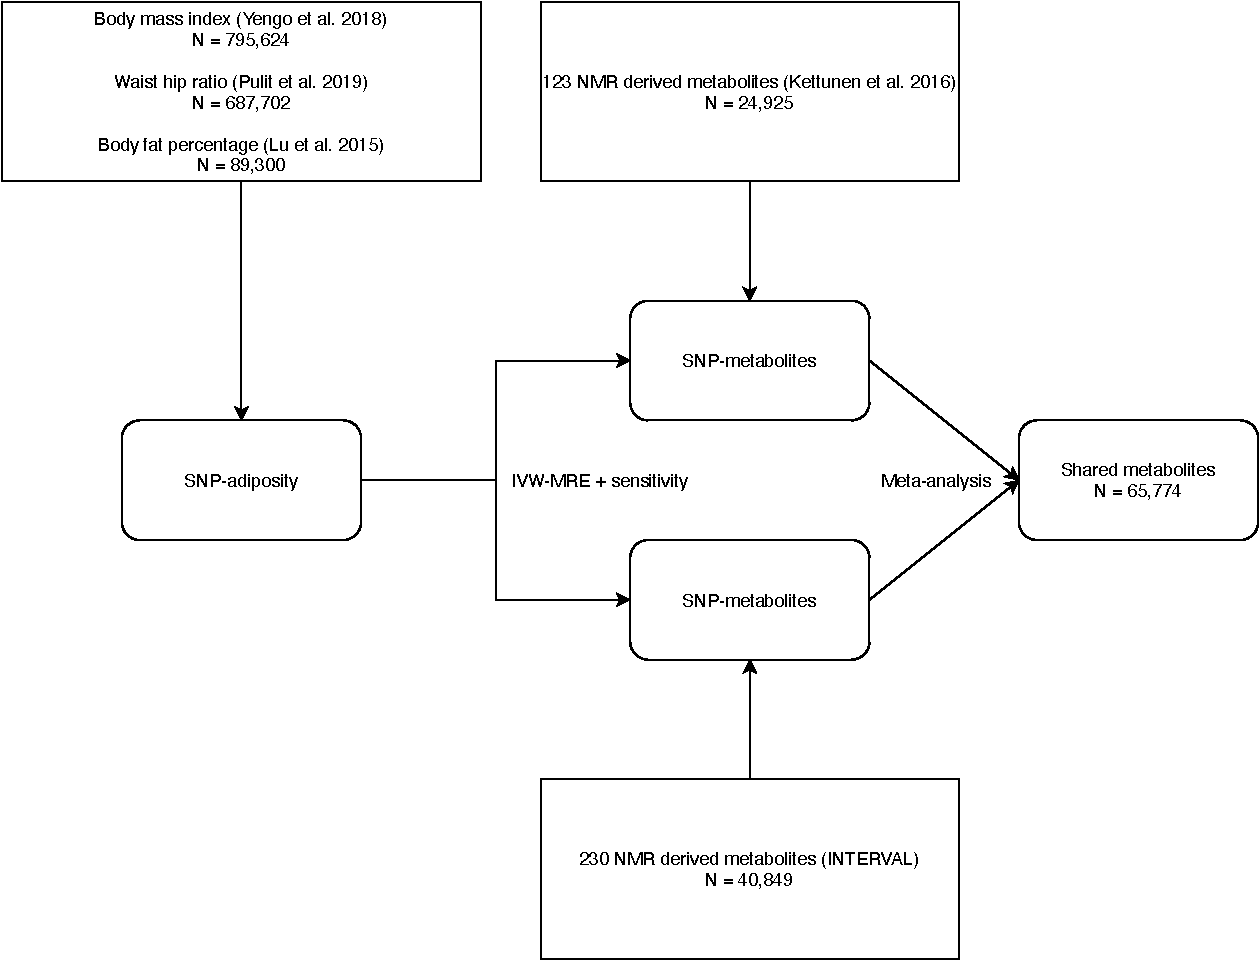
\includegraphics[width=1\linewidth]{../index/data/MR/figures/analysis_overview} \caption[Analysis overview]{\textbf{Analysis overview}. The main analysis consisted of two parallel two-sample Mendelian randomization (MR) analyses using three exposures (body mass index (BMI), waist hip ratio (WHR), and body fat percentage (BF)). Two outcome metabolomic datasets were used: (1) 123 nuclear magnetic resonance (NMR) derived metabolites measured in 24,925 individuals of European ancestries from the Kettunen et al., (2016) genome-wide association study (GWAS)\textsuperscript{\protect\hyperlink{ref-Kettunen2016}{335}}; (2) 230 NMR derived metabolites from 40,849 individuals of European ancestries from the INTERVAL GWAS. Four models were used: inverse variance weighted, multiplicative random effects (IVW-MRE) model was the main analysis; MR-Egger, weighted median, and weighted mode were used as sensitivity analyses. The number of SNPs used for each exposure along with the sample size (N) for the exposure and outcome datasets are given. A meta-analysis of the IVW-MRE results of 110 metabolites that were shared across the two studies was conducted.}\label{fig:MR-figure-analysis-flow}
\end{figure}
\hypertarget{MR-methods-instrumentation}{%
\subsection{Instrumentation}\label{MR-methods-instrumentation}}

Instrumentation of exposures is primarily achieved using either single genetic variants or multiple genetic variants as instrumental variables. A limitation of using a single genetic variant to instrument an exposure is that the proportion of variance explained in the exposure by that variant will likely be low (although some cases exist where variants near or in the protein coding region of the gene, known as cis-variants, that lead to changes in protein levels such as c-reactive protein). This can result in a weak instrument which can lead to biased estimates towards the confounded observational effect in a one-sample setting and towards the null in a two-sample setting\textsuperscript{\protect\hyperlink{ref-Davies2018}{358}}. Using multiple genetic instruments which, collectively, explain a greater proportion of the trait variance than any one individual variant can mitigate weak instrument bias.

\par

In Chapter \ref{systematic-review}, 173 studies which used a measure of adiposity as an exposure in 2,214 MR analyses were reviewed. The majority of these 2,214 MR analyses used BMI (N = 1,509) as the exposure; 112 analyses used WHR and 45 used BF, the remaining analyses used differing measures of fat mass and depositions such as hepatic fat. The majority of analyses used multiple instruments. In many instances, it was not possible to identify the exact instruments used due to an absence of information or missreporting. On the whole however, the main instrumentation strategy was to obtain instruments from the most recent GWAS with the largest sample size. This resulted in most analyses using a genome-wide significance threshold of p-value \textless{} 5 x 10\textsuperscript{-8}. Few studies discussed the independence of their genetic variants, and those that did mostly reported that the original GWAS declared the SNPs to be independent from one another - very few analyses performed clumping of their obtained instruments, i.e., used a linkage disequilibrium (LD) r\textsuperscript{2} and a distance threshold to identify independent SNPs. In order to allow comparison between results here and those previously reported, the instrumentation approach used most commonly in previous analyses was used in these analyses. For the main analysis here, instruments were obtained directly from the most recently published GWAS with the largest sample size. In additional analyses performed here, instruments were obtained from GWAS which did not use UK Biobank, due to potential concerns over population structure\textsuperscript{\protect\hyperlink{ref-Haworth2019}{366},\protect\hyperlink{ref-Lawson2020}{548}--\protect\hyperlink{ref-Sanderson2021}{550}}, and performed clumping of identified instruments to ensure consistency in the independence of instruments across exposures.

\par

\hypertarget{data}{%
\subsection{Data}\label{data}}

The following section details a number of GWAS and meta-analyses of previously published studies, which were used in this Chapter to perform MR analyses and are required as per STROBE-MR guidelines\textsuperscript{\protect\hyperlink{ref-DaveySmith2019}{440}}. I was not not directly involved in these GWAS. The total sample size (N) and sex-specific sample size does not always tally, this is due to variation in the sample size for each SNP. Where this is the case, `sample size up-to' is used. Due to the way in which studies report GWAS differently, information present in one study (such as sex-specific sample sizes) are not always present in another. As such, some information is missing from the GWAS described here in. Additional details, such as the methods used for individual GWAS which make up the meta-analyses presented here, are provided in the Appendix (\ref{appendix-MR-exposures}).

\par

\hypertarget{MR-exposures-adiposity}{%
\subsubsection{Exposures: measures of adiposity}\label{MR-exposures-adiposity}}

\hypertarget{body-mass-index}{%
\paragraph{Body mass index}\label{body-mass-index}}

Genetic variants robustly associated with BMI were extracted from Yengo et al., (2018)\textsuperscript{\protect\hyperlink{ref-Yengo2018}{53}}, who analysed data from 515,509--795,624 individuals of European ancestries from two sources, the Genetic Investigation of Anthropometric Traits (GIANT) consortium\textsuperscript{\protect\hyperlink{ref-Locke2015}{48}} and UK Biobank. In both sources, BMI was calculated as \(\displaystyle \frac{weight\ (kg)}{height\ (m^2)}\). Yengo et al., (2018)\textsuperscript{\protect\hyperlink{ref-Yengo2018}{53}} performed a fixed effects inverse variance weighted meta-analysis of BMI using GWAS results generated from UK Biobank (N = 456,426) and results from the GIANT consortium, Locke et al., (2015)\textsuperscript{\protect\hyperlink{ref-Locke2015}{48}} (N = 322,154) using METAL\textsuperscript{\protect\hyperlink{ref-Willer2010}{551}}.

\par

In UK Biobank, BMI was adjusted for age, sex, recruitment centre, genotyping batch, and the first 10 principal components (PCs) calculated from 132,102 (out of 147,604) genotyped SNPs pre-selected by the UK Biobank quality control team\textsuperscript{\protect\hyperlink{ref-Bycroft2018}{552}}. In GIANT, BMI was adjusted for age, age-squared, and study-specific covariables (e.g.~genotype-derived PCs). The residuals from both UK Biobank and GIANT were inverse rank normally transformed and represent SD units. In total, 681,275 individuals of European ancestries and \textasciitilde2.4 million HapMap Phase II imputed SNPs were included in the meta-analysis. The intercept for linkage disequilibrium score regression (\textsuperscript{I}LDSC = 1.03; SE = 0.02) suggested population stratification. However, LDSC can rise above 1 as sample sizes and heterogeneity increase\textsuperscript{\protect\hyperlink{ref-Loh2018}{553}}; therefore, this was unlikely to impact interpretation of GWAS results. Briefly, LDSC can estimate the contribution of confounding factors, such as population structure, on summary statistics based on a regression of the SNP effect estimates and linkage disequilibrium scores (LD r\textsuperscript{2}) of all other SNPs.

\par

In the meta-analysis, a total of 656 primary associations reaching a genome-wide significance threshold of p-value \textless{} 5 x 10\textsuperscript{-8} were identified. Approximate conditional and joint multiple-SNP (COJO) analysis, whereby secondary signals which are conditional on the presence of a primary signal are identified, identified a further 285 independent SNPs reaching an adjusted genome-wide significance threshold of p-value \textless{} 1 x 10\textsuperscript{-8}. Together, these 941 associations explain 6\% (SE = 0.8\%) and 22.4\% (SE = 3.7\%) of the variance and heritability of BMI respectively.

\par

All 941 SNPs identified in the COJO-GWAS were used in the main MR analysis of this chapter. Primary SNPs (N = 656) were identified as those with the smallest p-value within a 1 mega-base (Mb) window, secondary SNPs (COJO-specific SNPs = 256) were identified as conditional on the presence of a primary SNP given a p-value threshold of 1 x 10\textsuperscript{-8} and a 1Mb window.

\par

\hypertarget{waist-hip-ratio}{%
\paragraph{Waist hip ratio}\label{waist-hip-ratio}}

Genetic variants robustly associated with WHR were extracted from Pulit et al., (2019)\textsuperscript{\protect\hyperlink{ref-Pulit2019}{54}}, who analysed data from 485,486---697,702 individuals of European ancestries from two sources, UK Biobank and the GIANT consortium\textsuperscript{\protect\hyperlink{ref-Shungin2015}{49}}. In both sources, WHR was calculated as \(\displaystyle \frac{waist\ circumference\ (cm)} {hip\ circumference\ (cm)}\). Pulit et al., (2019)\textsuperscript{\protect\hyperlink{ref-Pulit2019}{54}} performed a fixed effects inverse variance weighted meta-analysis of WHR using GWAS results generated from UK Biobank (N up to 485,486 (men up to 263,148; women up to 222,338)) and results from the GIANT consortium (N up to 212,248 (men up to 94,434; women up to 118,004))\textsuperscript{\protect\hyperlink{ref-Shungin2015}{49}} using METAL.

\par

In UK Biobank, WHR was adjusted for sex, age, age-squared and assessment centre. In GIANT, WHR was adjusted for age, age-squared and study-specific covariables. The residuals from both UK Biobank and GIANT were inverse rank normally transformed and represent SD units. In GIANT, residuals were calculated for men and women separately. Prior to meta-analysis, SNPs with a minor allele frequency difference \textgreater{} 15\% between the two sources were removed. In the meta-analysis, a total of 316 associations reaching a genome-wide significance threshold of p-value \textless{} 5 x 10\textsuperscript{-9} were identified, where the p-value was adjusted to account for denser imputation data\textsuperscript{\protect\hyperlink{ref-Pulit2017}{554}}. Independence was determined using an LD r\textsuperscript{2} threshold \textgreater{} 0.05 and a 10Mb window; the genomic span of each LD-based clump was identified and a 1kb buffer was added up- and down-stream. Where windows overlapped, they were merged into a single locus resulting in the 316 lead SNPs. These associations explained 3\% of the phenotypic variance as calculated in an independent dataset (N = 7,721). SNP-based heritability across all SNPs was estimated to be 22.7\%. These genetic variants were used as genetic instrumental variables in the main MR analysis in this chapter.

\par

\hypertarget{body-fat-percentage}{%
\paragraph{Body fat percentage}\label{body-fat-percentage}}

Genetic variants robustly associated with BF were extracted from Lu et al., (2016)\textsuperscript{\protect\hyperlink{ref-Lu2016}{51}}, who analysed data from up-to 89,297 (men up to 44,429; women up to 45,525) individuals of European ancestries. BF was measured with with dual-energy X-ray absorptiometry (DXA) or bioelectircal impedance as described previously\textsuperscript{\protect\hyperlink{ref-Kilpelainen2011}{46}}. The number of individuals with BF measured by DXA and impedance was not reported. Lu et al., (2016)\textsuperscript{\protect\hyperlink{ref-Lu2016}{51}} performed a fixed effects inverse variance weighted meta-analysis of BF using two meta-analyses generated from a meta-analysis of genome-wide array GWAS (N = 65,831) and a meta-analysis of Metabochip array GWAS (N = 23,468) using METAL\textsuperscript{\protect\hyperlink{ref-Willer2010}{551}}.

\par

For each of the individual genome-wide array and Metabochip array studies, BF was adjusted for age, age-squared, and study-specific covariables (e.g.~genotype-based principle components and study centre) if necessary. For studies of unrelated individuals, residuals were calculated separately in men and women, and separately in cases and controls. For studies of family-based design,residuals were calculated in men and women together, and sex was additionally included in the model. The residuals were inverse rank normally transformed and represent SD units. For studies of family-based design, the family relatedness was additionally included in each GWAS. Each study performed study specific quality control. Imputation was performed in each study using the European ancestries HapMap Phase II (Release 22) reference panel. Analysis was then performed in three-stages. First, GWAS for each genome-wide array and Metabochip array study was performed using linear regression assuming an additive genetic model. Second, parallel meta-analysis of the genome-wide array GWAS and the Metabochip array GWAS were performed using a fixed effects inverse variance weighted model. Third, meta-analysis of these two meta-analyses was performed using a fixed effects inverse variance weighted model.

\par

In total 7 SNPs reached a genome-wide significance threshold (p-value \textless{} 5 x 10\textsuperscript{-8}) and were considered independent (± 500kb of the most significant SNP). Estimation of variance explained was not available in the European ancestries meta-analysis. In a meta-analysis of individuals of all ancestries, which included up to 11,419 additional individuals of non-European ancestries, these 7 SNPs explained 0.416\% of the variance in BF. The additional 5 SNPs identified in this all ancestries meta-analysis explained 0.58\% of the variance in BF. The 7 genetic variants, identified in the European ancestries meta-analysis, were used as genetic instrumental variables in main MR analysis in this chapter.

\par

\hypertarget{outcomes-metabolites-1}{%
\subsubsection{Outcomes: metabolites}\label{outcomes-metabolites-1}}

\hypertarget{kettunen-et-al.-2016kettunen2016}{%
\paragraph{\texorpdfstring{Kettunen et al., (2016)\textsuperscript{\protect\hyperlink{ref-Kettunen2016}{335}}}{Kettunen et al., (2016)335}}\label{kettunen-et-al.-2016kettunen2016}}

Genome-wide summary level data for 123 NMR-derived metabolites, which includes derived metabolite measures (Appendix Table \ref{tab:appendix-MR-table-metabolites}), were available from Kettunen et al., (2016)\textsuperscript{\protect\hyperlink{ref-Kettunen2016}{335}}. In total, metabolomic data were available for up-to 24,925 individuals of European ancestries. Metabolomic data were from the comprehensive quantitative serum/plasma platform described by Soininen et al., (2009)\textsuperscript{\protect\hyperlink{ref-Soininen2009}{514}}, the same platform used in Chapter \ref{observational}. Kettunen et al., performed a fixed effects meta-analysis of 123 serum and Ethylenediaminetetraacetic acid (EDTA) plasma NMR quantified metabolites from 14 GWAS.

\par

For each of the 14 cohorts contributing to the 14 GWAS, 123 shared metabolites were quantified from human blood. Four cohorts used EDTA-plasma, the other 10 used serum. The majority of blood samples were fasted. Where a study did not have over-night fasted samples, correction for fasting time effect was performed using the \texttt{gam} \texttt{R} package and fitting a smoothed spline to adjust for fasting. All metabolites were adjusted for age, sex, time from last meal if applicable, and the first ten PCs. The residuals for each adjusted metabolite were inverse rank normally transformed and represent SD units. Each of the 14 cohorts performed a univariate GWAS assuming an additive genetic model. SNPs were imputed up to 39 million markers using the 1000 Genomes Project, March 2012 version.

\par

For the meta-analysis, SNPs with accurate imputation (info \textgreater{} 0.4) and minor allele count \textgreater{} 0.3 were combined using double genomic control correction, that is, both individual cohort results and meta-analysis results were corrected for the genomic inflation factor as implemented in \texttt{GWAMA}. Up to 12,133,295 SNPs were included in the meta-analysis. Variants present in more than seven studies after filtering and meta-analysis were considered for the final results. All traits gave genomic inflation factors in the meta-analysis \textless{} 1.034 showing little evidence of systematic bias in the test statistic. A genome-wide significance threshold (p-value \textless{} 2.27 x 10\textsuperscript{-9}) after correcting for 22 independent tests (22 being the number of principal components explaining over 95\% of variation in the metabolite data) was used. These filtered summary statistics were used in MR analyses in this Chapter to extract adiposity-related genetic variants.

\par

\hypertarget{interval}{%
\paragraph{INTERVAL}\label{interval}}

Genome-wide summary level data for 230 NMR-derived metabolites, which includes derived metabolite measures (Appendix Table \ref{tab:appendix-MR-table-metabolites}), were available from the INTERVAL study. INTERVAL is a randomised trial of \textasciitilde50,000 individuals recruited from June 2012--June 2014 in the United Kingdom to investigate the safety of different blood donation intervals\textsuperscript{\protect\hyperlink{ref-Moore2014b}{545}}. In total, metabolomic data were available for up up to 40,849 individuals of European ancestries. Metabolomic data were from the comprehensive quantitative serum/plasma platform described by Soininen et al., (2009)\textsuperscript{\protect\hyperlink{ref-Soininen2009}{514}}, the same platform used for the Kettunen dataset and metabolomic data in Chapter \ref{observational}. A linear mixed model (LMM) GWAS of 230 serum NMR quantified metabolites was performed using BOLT-LMM. The INTERVAL GWAS data were unpublished and provided by collaborators (Adam Butterworth, University of Cambridge).

\par

Samples or analytes with potentially unreliable data were flagged. Flagged metabolites included acetate, pyruvate, glucose, and lactate. Individuals with flagged values for any of these metabolites had those values set to missing. Individuals were excluded if they had \textgreater{} 30\% analyte missingness, and one NMR PC outlier. All metabolites were then log transformed and metabolites with values of 0 or values \textgreater{} 10 SD from the mean after log transformation were set to missing. Log transformed metabolite values were then adjusted for age, sex, recruitment centre, time between blood draw and sample processing, and the first 10 PCs of genetic ancestry. Residuals were then inverse rank normally transformed and represent log SD units.

For the GWAS, SNPs were imputed using a combined 1000 Genomes + UK10K panel, which captured 87,696,910 variants. A LMM was fit using BOLT-LMM. Variants that were poorly imputed (info score \textless{} 0.3 or R\textsuperscript{2} \textless{} 0.3), variants with unrealistic results (e.g.~standard error \textless{} 0, standard error \textgreater{} 10, beta = infinity), and variants with minor allele count \textless{} 5 were excluded. A genome-wide significance threshold was not set. A total of 28 PC explained over 95\% of variation in the metabolite data. These filtered summary statistics were used in MR analyses in this Chapter to extract adiposity-related genetic variants.

\par

\hypertarget{two-sample-mendelian-randomization-association-between-complimentary-measures-of-adiposity-and-metabolites}{%
\subsection{Two-sample Mendelian randomization: association between complimentary measures of adiposity and metabolites}\label{two-sample-mendelian-randomization-association-between-complimentary-measures-of-adiposity-and-metabolites}}

For all exposures, the following summary-level data were obtained from the original GWAS publications for each exposure-related genetic variant: rsID, effect allele, other/non-effect allele, effect allele frequency, effect estimate, standard error of the effect estimate, p-value, sample size, and units. The same data for these adiposity-related genetic variants were obtained for each metabolite separately from both Kettunen et al., and INTERVAL sources. Clumping of SNPs was not performed as the studies from which they were obtained stated they were independent or near-independent and had already been clumped. To assess the possibility of weak instrument bias, F-statistics were calculated for each SNP and an average F-statsistic was calculated for each exposure.

\par

Genetic variants were extracted from each metabolite GWAS and, where these were not present, proxy SNPs were included if LD was \(\geq\) 0.8. For proxy SNPs, the inclusion of SNPs where the reference strand was ambiguous (strand flips) was allowed and the reference strand was inferred using a minor allele frequency (MAF) threshold. That is, the reference strand was inferred using a MAF, so long as that MAF was not \(\geq\) 0.3, in which case it was excluded. Exposure and outcome summary statistics for each of the adiposity-related SNPs were harmonised in reference to the exposure effect allele being on the increasing scale. For included alleles where the reference strand was ambiguous, the positive strand was inferred using effect allele frequency. That is, if the effect allele frequency of a SNP was not \(\geq\) 0.3 or \(\leq\) 0.7, the reference strand was inferred using the effect allele frequency to harmonise exposure and outcome data; otherwise, it was removed.

\par

An inverse variance weighted (IVW), multiplicative random effects (IVW-MRE) model was used to investigate the effect of each exposure on each metabolite. The model assumes that the strength of the association between the genetic instruments and the exposure is not correlated with the magnitude of pleiotropic effects and, that pleiotropic effects have an average value of zero\textsuperscript{\protect\hyperlink{ref-Bowden2017}{555}}. Pleiotropy, discussed in Chapter \ref{introduction} Section \ref{mendelian-randomization}, describes the phenomena in which a SNP has an effect on multiple traits. Specifically in regards to MR analyses, it describes the phenomena in which SNPs associated with the exposure (e.g., adiposity) are also associated with the outcome (e.g., metabolites) through pathways (e.g., cardiovascular disease) that are not via the exposure.

\par

Multiple testing thresholds correcting for the number of independent tests between adiposity and metabolites being undertaken with MR analyses were applied when using the Kettunen and INTERVAL data. For the Kettunen data, a multiple testing threshold of p-value \textless{} 0.0023 was applied; this is based on the number of principal components (22) in the Kettunen et al., meta-analysis that explained 95\% of the variation in metabolite data. For the INTERVAL data, a multiple testing threshold of p-value \textless{} 0.0018 was applied; this is based on the number of principal components (28) in the INTERVAL GWAS that explained 95\% of the variation in metabolite data.

\par

For MR analyses using the Kettunen et al., (2016) data, effect estimates are given in SD units per SD higher BMI, WHR, or BF. For MR analyses using the INTERVAL data, effect estimates are given in log SD units per SD higher BMI, WHR, or BF. The metabolic profile of adiposity was visualised using Circos plots made with the \texttt{EpiViz} \texttt{R} package (detailes in Chapter \ref{visualisation}). Directions of effect were compared across exposures for analysis using Kettunen data and analysis using INTERVAL data. Tests which reached a multiple testing threshold within each analysis are presented and the effect of adiposity on subclasses was explored in regard to the multiple testing threshold.

\par

\hypertarget{MR-sensitivity}{%
\subsubsection{Sensitivity analyses}\label{MR-sensitivity}}

Where possible, the assumptions of no pleiotropy among genetic instruments and outcomes were explored using: MR-Egger\textsuperscript{\protect\hyperlink{ref-Bowden2015}{368}}, weighted median\textsuperscript{\protect\hyperlink{ref-Burgess2017a}{369}}, and weighted mode\textsuperscript{\protect\hyperlink{ref-Hartwig2017}{370}} based estimators. Sensitivity analysis was performed for all exposure-outcome pairs, but focus was given to those pairs which met a multiple testing threshold in the main analysis. For these sensitivity models, no threshold requirements were set, instead, consistency in the direction of effect estimates and the presence of overlapping confidence intervals (CIs) between the IVW-MRE model and these methods was investigated.

\par

MR-Egger provides an estimate of unbalanced/directional horizontal pleiotropy via the intercept of a linear regression of the SNP-exposure and SNP-outcome association. In the presence of pleiotropy the intercept will be biased away from the origin. MR-Egger gives consistent estimates when 100\% of genetic instruments are invalid\textsuperscript{\protect\hyperlink{ref-Bowden2015}{368}}. The weighted median is complimentary to MR-Egger but does not rely on the ``instrument strength independent of direct effect'' (InSIDE) assumption. It calculates the median of an empirical distribution of the causal effect estimates weighted for precision. It provides consistent estimates when at least 50\% of the weight comes from valid genetic instruments and as long as no one genetic instrument contributes \textgreater{} 50\% of the weight\textsuperscript{\protect\hyperlink{ref-Burgess2017a}{369}}. The weighted mode assumes the true causal effect is the most common effect, it is robust when the majority of effect estimates are derived from valid instruments\textsuperscript{\protect\hyperlink{ref-Hartwig2017}{370}}. The effects of heterogeneity in the exposure instruments was investigated using Cochran's Q statistic for IVW-MRE and MR-Egger models.

\par

In these analyses, it is assumed that the instruments influence the exposure first and their effect on the outcome through the exposure is secondary. Given the large number of genetic instruments used, as well as the feed-back and feed-forward loops present in the metabolome, the directionality of association may be difficult to evaluate. For example, a SNP which is strongly associated with adiposity may also have an effect on the metabolite under investigation via an association between that SNP and another metabolite which is up- or down-stream of that metabolite. The Steiger test\textsuperscript{\protect\hyperlink{ref-Hemani2017}{556}}, applied here using the \texttt{TwoSampleMR} package, can be used to estimate whether the test under investigation is the ``true'' causal direction. The Steiger test calculates the variance explained in the exposure and the variance explained in the outcome by the exposure-related instruments. If the variance explained in the outcome is less than that explained in the exposure, then the direction of effect can be considered to be from the exposure to the outcome. However, if the variance explained in the outcome is more than that explained in the exposure, this may indicate an invalidation of the core MR assumptions but does not indicate that the direction of association is from the outcome to the exposure. In order to estimate the variance explained the N is required. For the Kettunen dataset, the sample size for each individual SNP was available. For the INTERVAL dataset, the overall sample size (N = 40,849) was used as the individual SNP sample sizes were not available.

\par

The Wald ratio estimator was used to generate causal effect estimates of each adiposity exposure on each metabolite for each SNP independently in a single-SNP MR. In addition, a ``leave-one-out'' sensitivity analysis, whereby an MR analysis where each SNP is sequentially left out and the causal effect estimated absent of that SNP, was performed using the IVW model. If the estimated effect is substantially altered after the removal of a single-SNP, this may imply that SNP is driving the association between the exposure and outcome, which may be indicative of a pleiotropic effect of that SNP. Finally, each of these sensitivity analyses were visualised using funnel plots and forest plots of the single-SNP and leave-one-out MR analyses to identify potential pleiotropic effects.

\par

\hypertarget{additional-analyses}{%
\subsubsection{Additional analyses}\label{additional-analyses}}

Whilst the main analyses employed the most common approach of identifying and using genetic variants as instruments in MR studies (i.e., taking exposure-related variants from the largest and most recent GWAS), there are a number of potential limitations to this approach within the context of this chapter. Firstly, genetic instrumental variables for BMI and WHR were obtained from studies using UK Biobank, which has shown evidence of latent population structure\textsuperscript{\protect\hyperlink{ref-Haworth2019}{366},\protect\hyperlink{ref-Berg2019}{367}}. BF instruments were obtained from a study which used different measures of BF, potentially leading to measurement heterogeneity, and two of the included SNPs have also been associated previously with `favourable adiposity' and may therefore not be reflections of increased total body fat\textsuperscript{\protect\hyperlink{ref-Yaghootkar2014}{47},\protect\hyperlink{ref-Yaghootkar2016}{557}}. To further test the validity of the genetic variants used in the main analyses as instruments, a complementary set of genetic instrumental variables for each adiposity measure were obtained from alternative published summary statistics (Table of instruments available on \href{https://github.com/mattlee821/000_thesis/blob/master/index/data/MR/tables/exposure_SNPs.txt}{GitHub}).

\par

Briefly, SNPs for BMI were obtained from the initial non-COJO analysis by Yengo et al., (2018)\textsuperscript{\protect\hyperlink{ref-Yengo2018}{53}} (N SNPs = 656), and a separate set of SNPs were obtained from Locke et al., (2015)\textsuperscript{\protect\hyperlink{ref-Locke2015}{48}} (N = 77) - which did not use UK Biobank; for WHR, SNPs were obtained from Shungin et al., (2015)\textsuperscript{\protect\hyperlink{ref-Shungin2015}{49}} (N SNPs = 26) - which did not use UK Biobank; for BF, the two SNPs associated with `favourable adiposity' were removed (N SNPs = 5) and an additional SNP set was identified in a GWAS using a single measure of BF from Hubel et al., (2019)\textsuperscript{\protect\hyperlink{ref-Hubel2019}{55}} (N SNPs = 76). Outcome data extraction and harmonisation was performed as for the main analysis. F-statistics (Appendix Section \ref{appendix-MR-fstatistics}) and detailed information on each additional exposure is available in the Appendix, Section \ref{appendix-MR-exposures}. The main analysis (IVW-MRE) and sensitivity analyses were re-run using these additional SNP lists.

\par

In addition, studies used a variety of methods and definitions of independence for SNPs. In order to ensure SNPs were independent to the same degree across all studies, genetic instrumental variables for all exposures (those used in the main analysis and in additional analyses described here) were clumped and the main analysis (IVW-MRE) and sensitivity analyses were re-run using these clumped instruments. Clumping was performed using the \texttt{R} package \texttt{TwoSampleMR}\textsuperscript{\protect\hyperlink{ref-Hemani2018}{547}} setting an LD r\textsuperscript{2} threshold of 0.001 for SNPs within a 10,000 base window of each other. Spearman's correlation between MR results from the non-clumped and clumped SNP lists was performed.

\par

\hypertarget{meta-analysis-of-two-sample-mendelian-randomization-results}{%
\subsection{Meta-analysis of two-sample Mendelian randomization results}\label{meta-analysis-of-two-sample-mendelian-randomization-results}}

Metabolomics data from Kettunen et al., (2016)\textsuperscript{\protect\hyperlink{ref-Kettunen2016}{335}} were inverse rank normally transformed prior to GWAS. For INTERVAL, metabolomics data were log transformed and then inverse rank normally transformed prior to GWAS. As these transformations use different scales, meta-analysis using MR effect estimates was not appropriate. Instead, a meta-analysis of each exposure-outcome pair was performed with p-values using the \texttt{metap} (version 1.4) \texttt{R} package using Fisher's method for combining p-values. Meta-analysis of the IVW-MRE results from the main analysis was performed.

\par

Fisher's method \eqref{eq:fishers-method} combines p-values from each test into one test statistic (\(X^2\)), where \(p_i\) is the p-value for the \(i\)\textsuperscript{th} test, \(k\) is the number of tests, and \(2k\) is the degrees of freedom. When all the null hypotheses are true, and the \(p_i\) are independent, \(X^2\) has a chi-squared distribution with \(2k\) degrees of freedom.

\par
\begin{equation}
  X^2_{2k} \sim -2 \sum_{i=1}^{k}ln(p_i), 
  \label{eq:fishers-method}
\end{equation}
A large chi-squared statistic compared to the degrees of freedom (with a corresponding low p-value) provides evidence of an effect in at least one study. The null hypothesis for each MR analysis is that there is no effect of adiposity on metabolites. The meta-analysis null hypothesis is that each tests null hypothesis is true. That is, the null hypothesis when using the Kettunen dataset (one test) and the null hypothesis when using the INTERVAL dataset (one test) are both true. The alternative hypothesis is that at least one of these tests null hypotheses is true. As such, acceptance of the null hypothesis (that there is weak evidence for an association between adiposity and metabolites in the meta-analysis) should not be interpreted as evidence of no effect in all studies. Given only two studies are included in any one exposure-outcome pair in the current work, the potential effects of heterogeneity are difficult to interpret and are therefore not focussed on here. Meta-analysis results are presented as directions of effect and p-values. A Bonferroni corrected p-value threshold accounting for the total number of independent metabolites able to be meta-analysed (p \textless{} 0.00045; 0.05/110) was used to identify evidence of an association.

\par

\hypertarget{comparison-of-two-sample-mendelian-randomization-and-observational-results-from-chapter-refobservational}{%
\subsection{Comparison of two-sample Mendelian randomization and observational results from Chapter \ref{observational}}\label{comparison-of-two-sample-mendelian-randomization-and-observational-results-from-chapter-refobservational}}

Metabolites included in the meta-analysis, which showed consistent directions of effect when using the Kettunen and INTERVAL data and which reached a Bonferroni corrected meta-analysis p-value threshold, were compared with observational results from Chapter \ref{observational}. Direction of effect in the meta-analysis was compared with direction of effect in the observational analysis to triangulate evidence, where consistency across methods improved confidence in causal effects.

\par

\hypertarget{MR-results}{%
\section{Results}\label{MR-results}}

The effects of BMI, WHR, and BF on a total of 123 metabolites using data from Kettunen et al., (2016)\textsuperscript{\protect\hyperlink{ref-Kettunen2016}{335}} and 230 metabolites using data from INTERVAL were estimated using an IVW-MRE model. F-statistics for all SNPs used as genetic instruments for each exposure were above 10 (mean F-statistics: BMI = 73, WHR = 66, BF = 44; Table of SNPs available on \href{https://github.com/mattlee821/000_thesis/blob/master/index/data/MR/tables/exposure_SNPs.txt}{GitHub}).

\par

For MR analyses using the Kettunen et al., (2016) metabolites, effect estimates are given in SD units per SD higher BMI, WHR, or BF. For MR analyses using the INTERVAL metabolites, effect estimates are given in log SD units per SD higher BMI, WHR, or BF. Metabolites are grouped into subclasses to aid interpretation of results. The Kettunen dataset included two subclasses (metabolites ratio and protein) which were not present in the INTERVAL data. In the INTERVAL data, 16 subclasses, which were all derived metabolic measures (i.e.~ratios of one measured metabolite to another), were not available in the Kettunen data.

\par

\hypertarget{two-sample-mendelian-randomization-association-between-complimentary-measures-of-adiposity-and-metabolites-1}{%
\subsection{Two-sample Mendelian randomization: association between complimentary measures of adiposity and metabolites}\label{two-sample-mendelian-randomization-association-between-complimentary-measures-of-adiposity-and-metabolites-1}}

\hypertarget{metabolic-profile}{%
\subsubsection{Metabolic profile}\label{metabolic-profile}}

Effect estimates from the IVW-MRE model showed evidence for a broad effect of adiposity on the metabolic profile (Figure \ref{fig:MR-figure-circosplot-kettunen-main-analysis} and \ref{fig:MR-figure-circosplot-interval-main-analysis}). The pattern of association was visually similar when using the Kettunen data for BMI and WHR, and when using the INTERVAL data for BMI and WHR. When using the Kettunen data, the effect of BF on metabolites was visually distinct to the effect of BMI and WHR, with many effect estimates appearing to be inverse to those for BMI and WHR. However, when using the INTERVAL data, the effect of BF looked more similar in regards to the direction of effect to that of BMI and WHR. However, these effects appeared to cross the null much more often. Effects for WHR were generally larger with wider CIs, whereas those for BMI were smaller with tighter CIs. Effects for BF were much larger across both metabolite datasets, with wide CIs which spanned the null. A table of results for analyses using \href{https://github.com/mattlee821/000_thesis/blob/master/index/data/MR/results/mr_results_kettunen.txt}{Kettunen} and \href{https://github.com/mattlee821/000_thesis/blob/master/index/data/MR/results/mr_results_interval.txt}{INTERVAL} data are available on GitHub.

\par

\newpage




\begin{figure}

{\centering 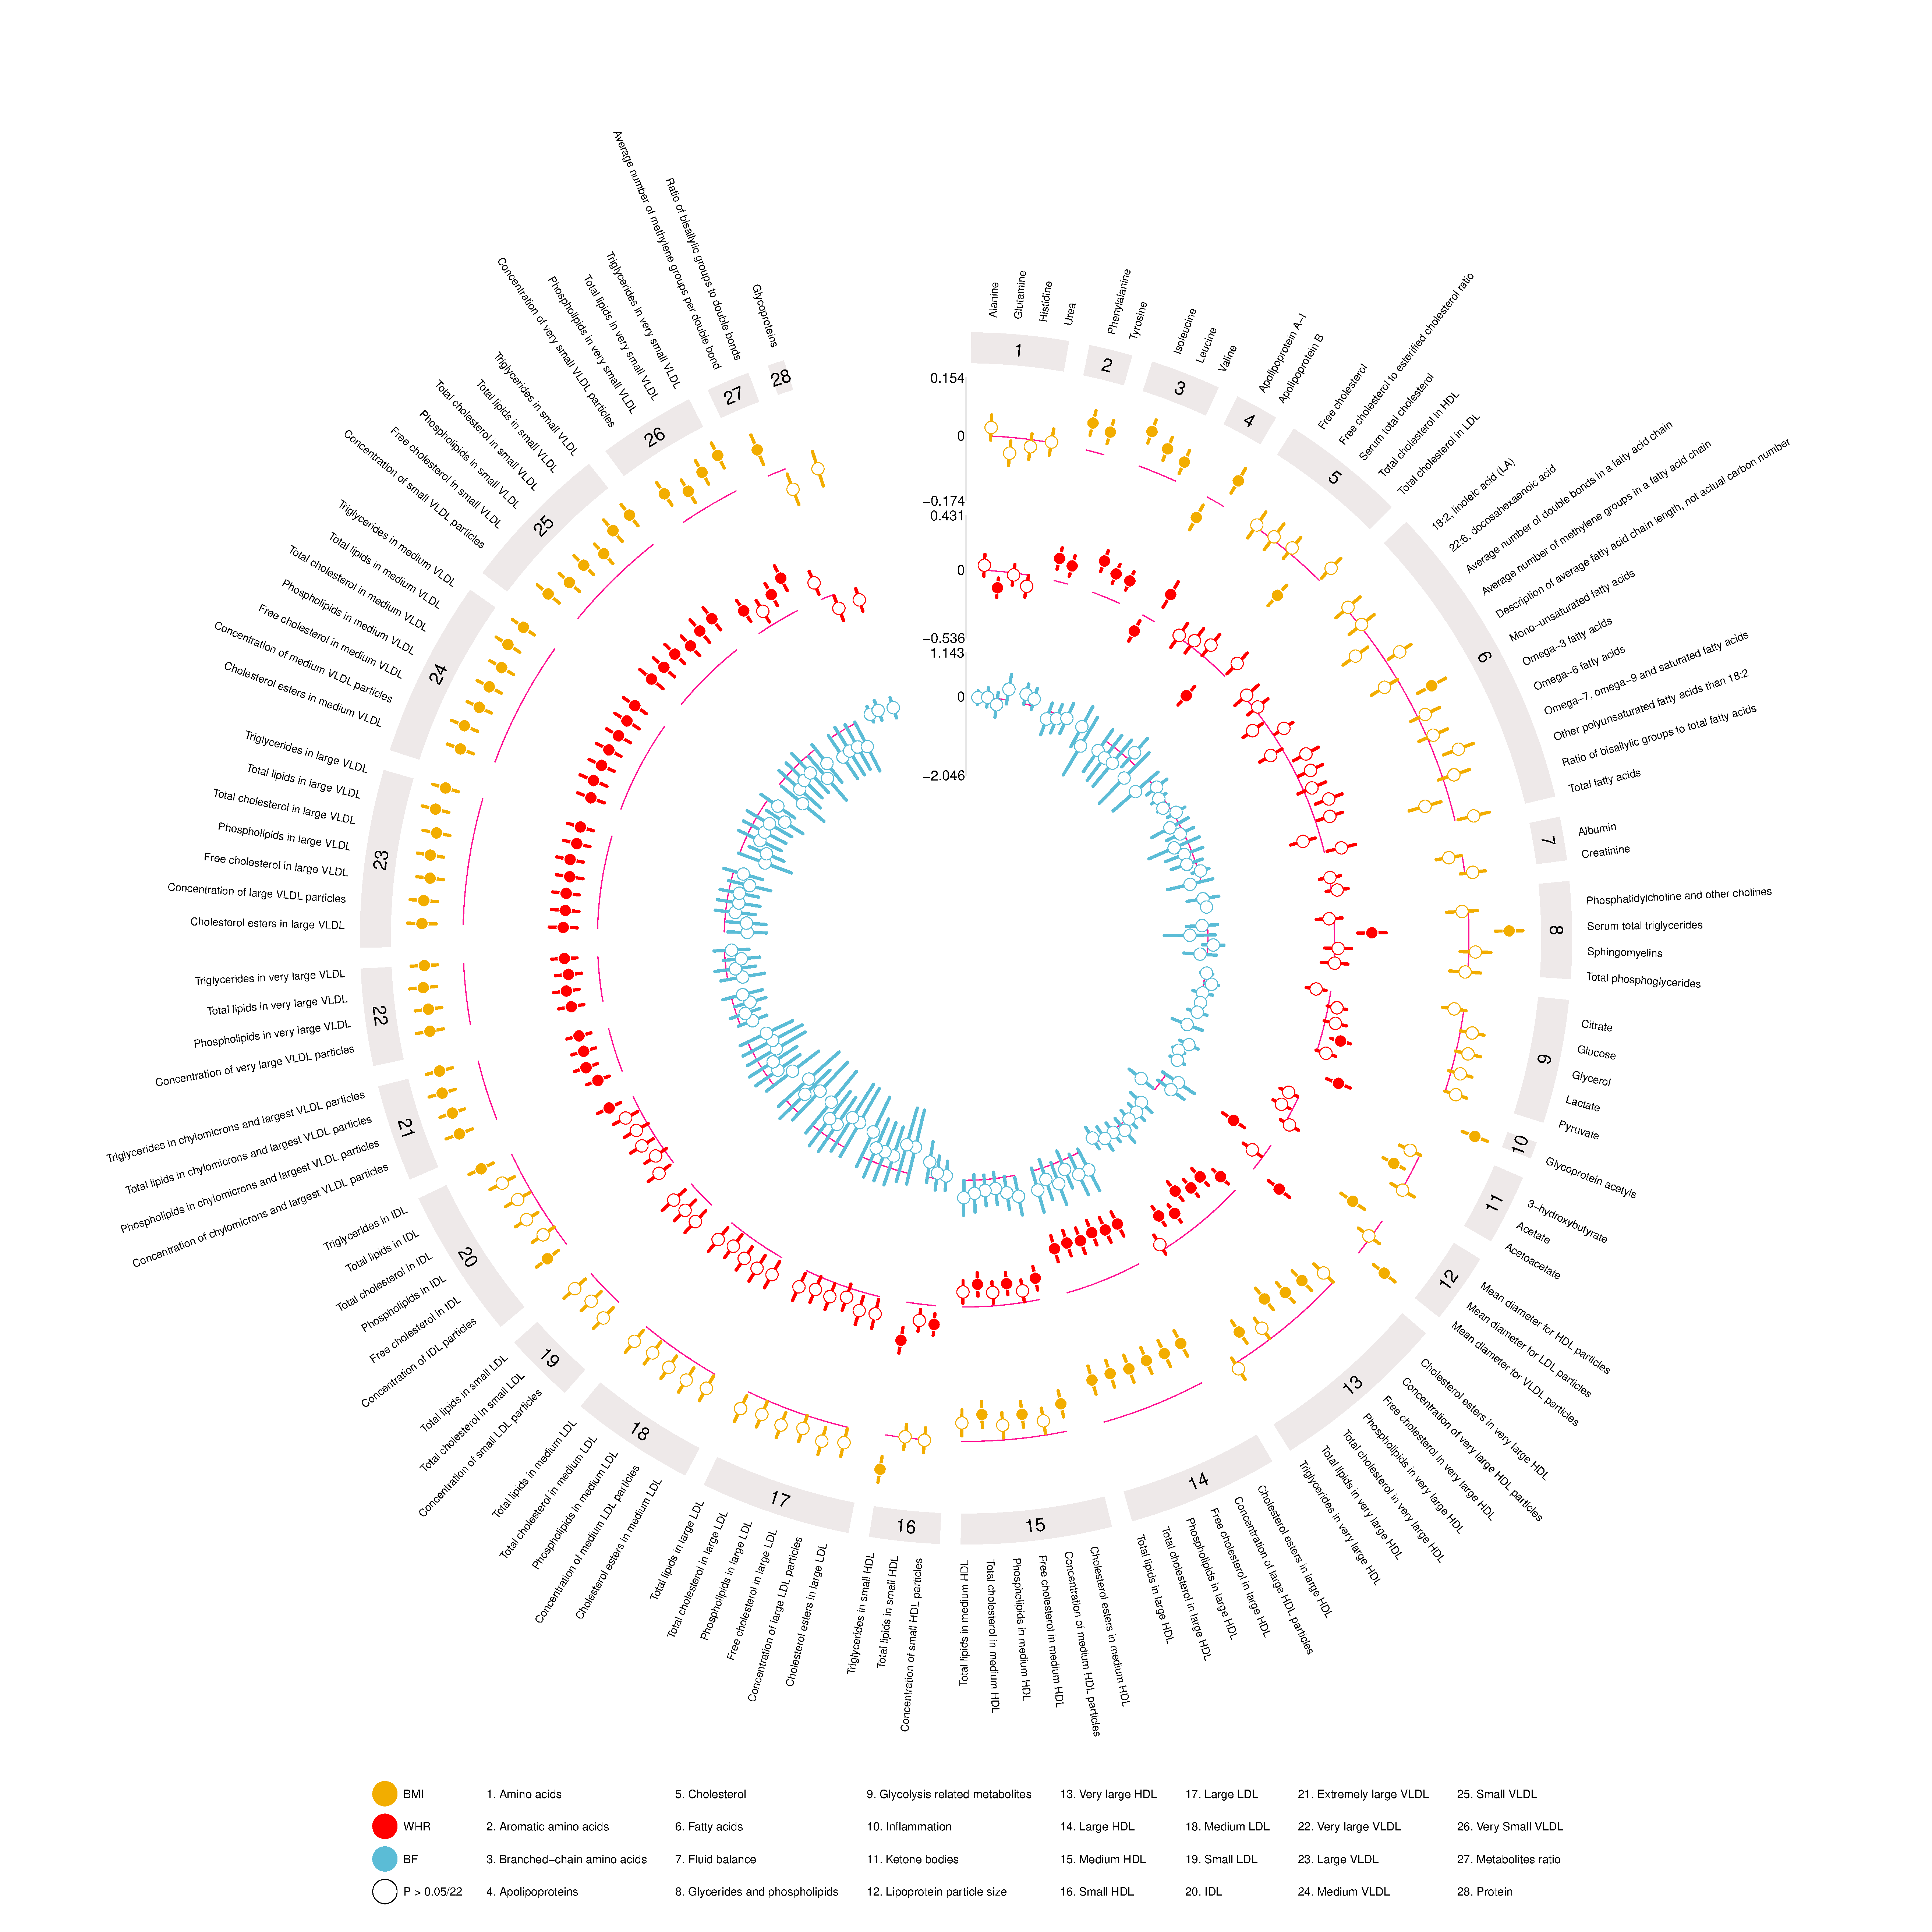
\includegraphics[width=1\linewidth]{data/MR/figures/circosplot_kettunen_main_analysis} 

}

\caption[Mendelian randomization analysis: association between adiposity measures and metabolites using Kettunen data]{\textbf{Mendelian randomization analysis: association between adiposity measures and metabolites using Kettunen data}. Circos plot shows each track as one measures of adiposity; the outer track is body mass index (BMI), the middle track is waist hip ratio (WHR), the inner track is body fat percentage (BF). Solid points indicate a multiple testing threshold (0.0023) has been reached. Effect estimates are given in SD units per SD higher BMI, WHR, or BF. 95\% confidence intervals shown. Metabolites are grouped by subclass and arranged alphabetically within each subclass. Available on \href{https://github.com/mattlee821/000_thesis/blob/master/index/data/MR/figures/circosplot_kettunen_main_analysis.pdf}{GitHub}.}\label{fig:MR-figure-circosplot-kettunen-main-analysis}
\end{figure}
\newpage




\begin{figure}

{\centering 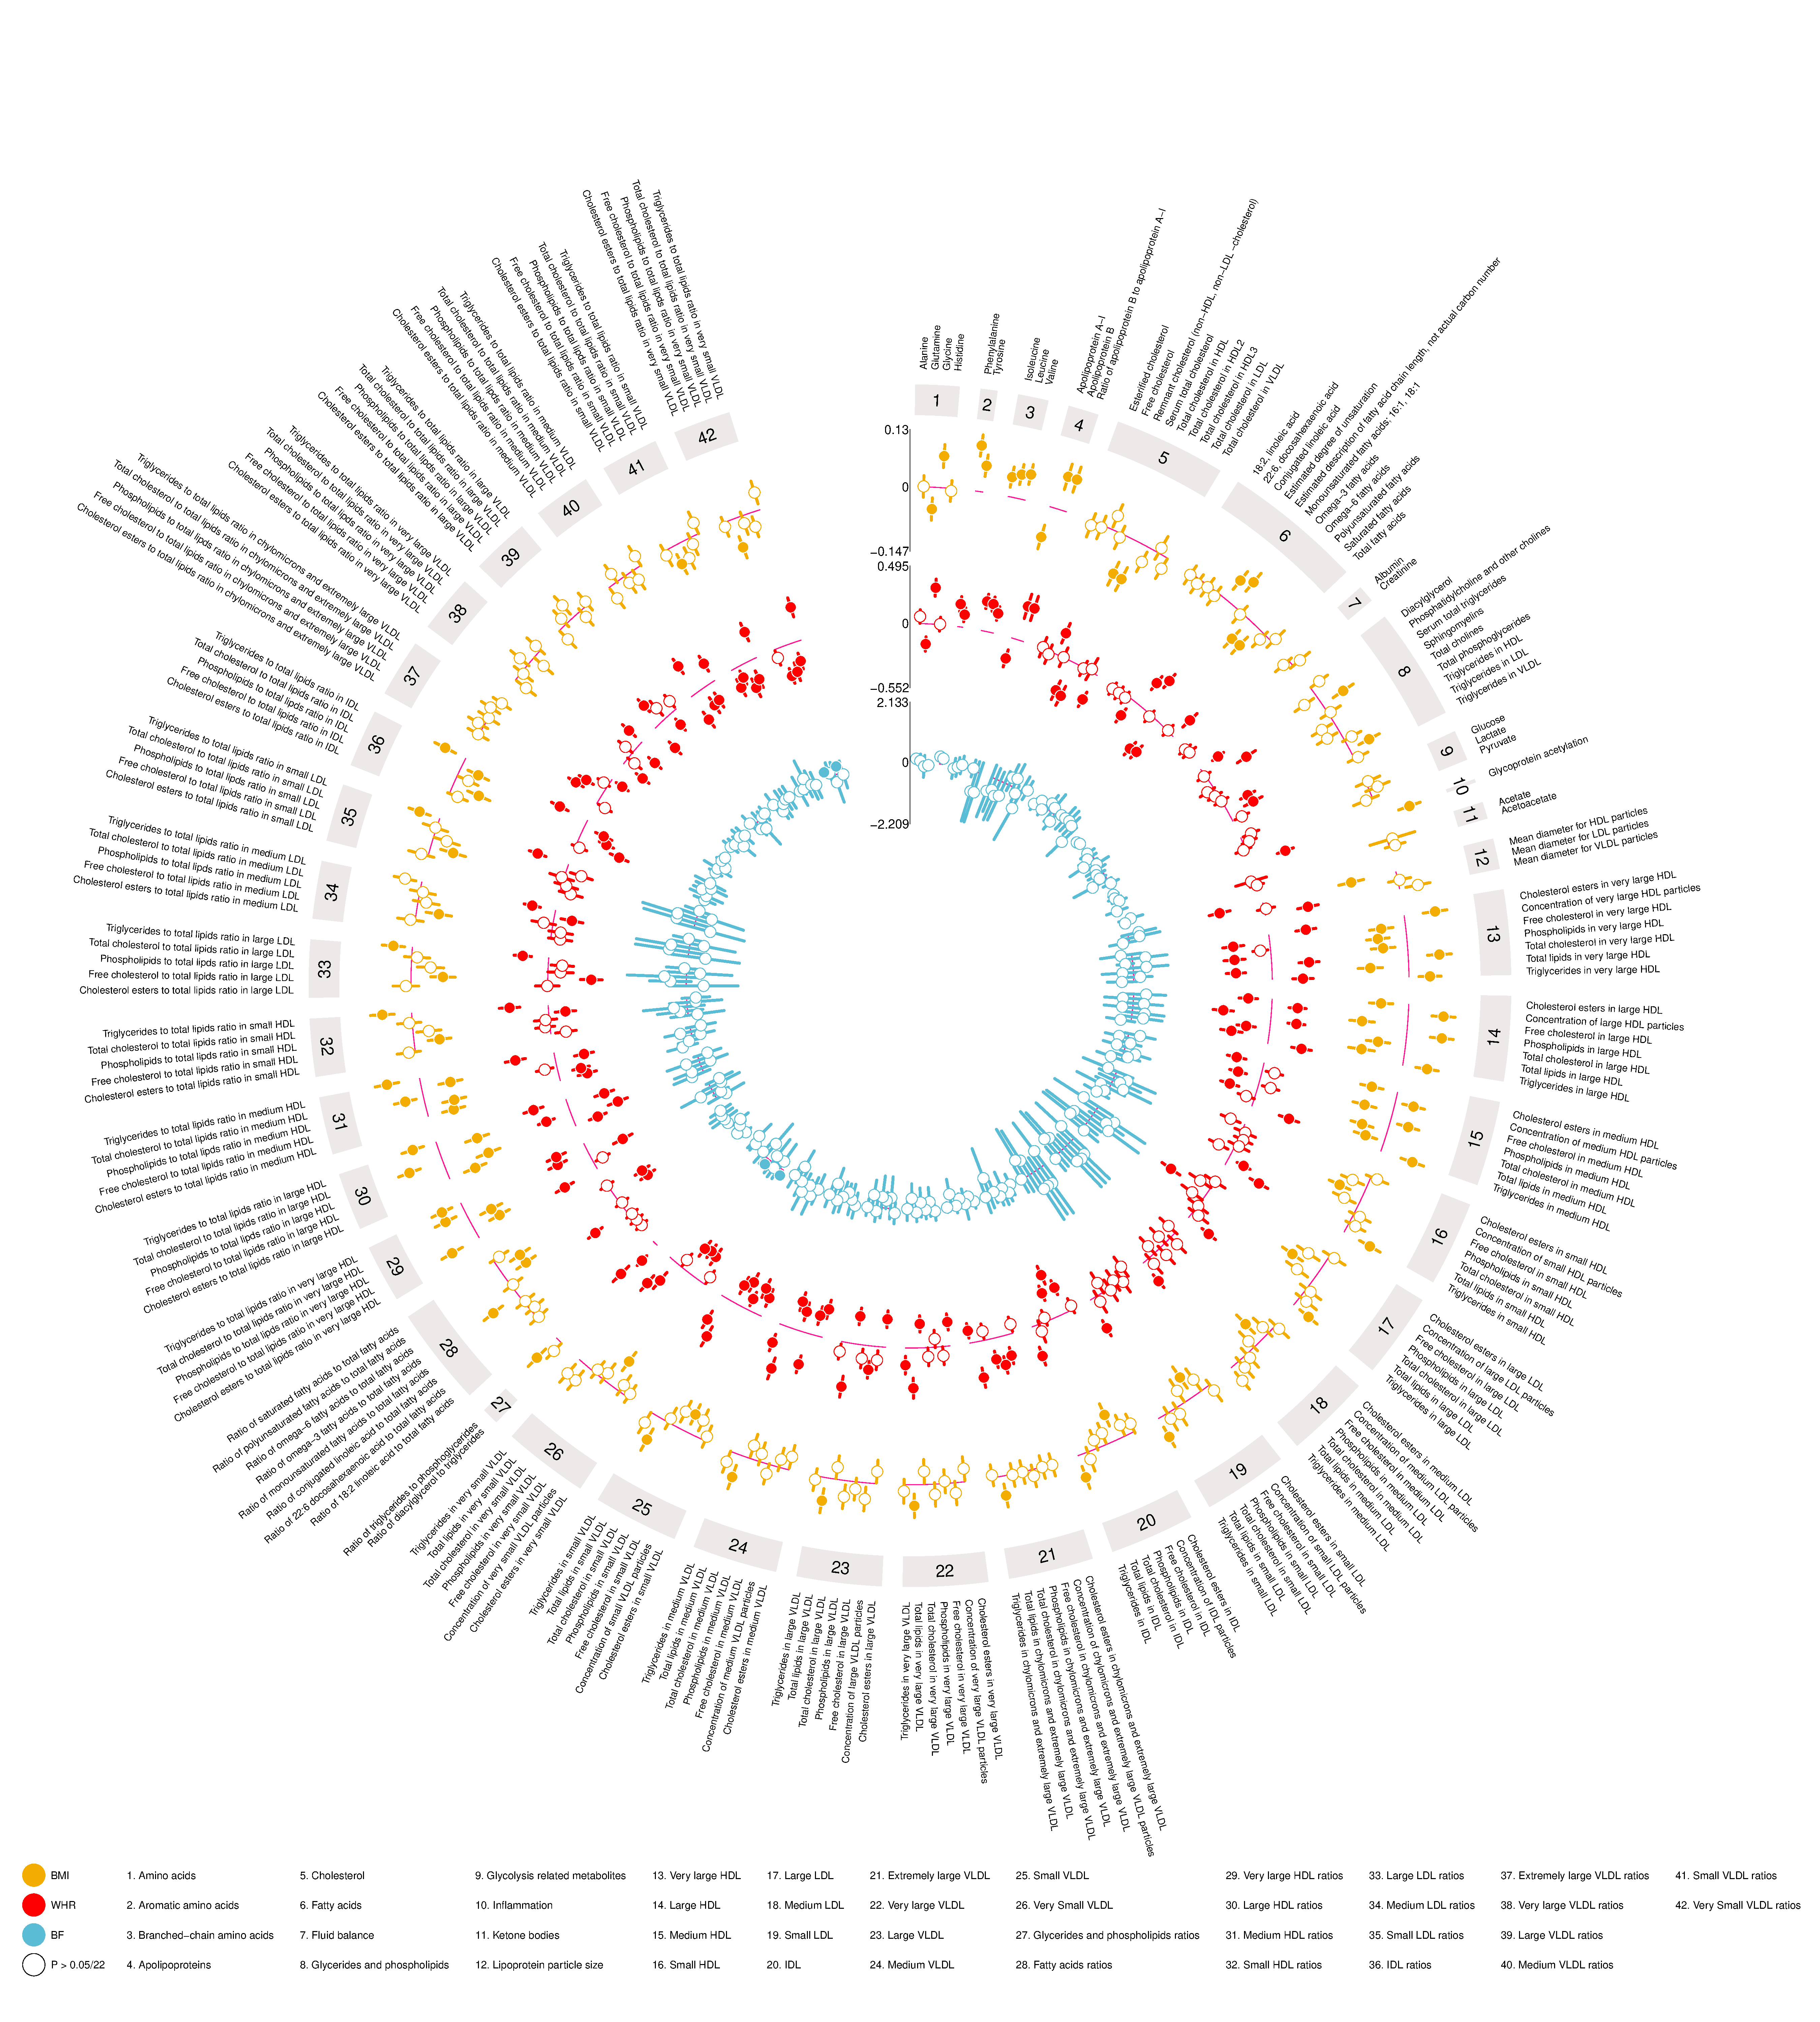
\includegraphics[width=1\linewidth]{data/MR/figures/circosplot_interval_main_analysis} 

}

\caption[Mendelian randomization analysis: association between adiposity measures and metabolites using INTERVAL data]{\textbf{Mendelian randomization analysis: association between adiposity measures and metabolites using INTERVAL data}. Circos plot shows each track as one measures of adiposity; the outer track is body mass index (BMI), the middle track is waist hip ratio (WHR), the inner track is body fat percentage (BF). Solid points indicate a multiple testing threshold (0.0018) has been reached. Effect estimates are given in log SD units per SD higher BMI, WHR, or BF. 95\% confidence intervals shown. Metabolites are grouped by subclass and arranged alphabetically within each subclass. Available on \href{https://github.com/mattlee821/000_thesis/blob/master/index/data/MR/figures/circosplot_interval_main_analysis.pdf}{GitHub}.}\label{fig:MR-figure-circosplot-interval-main-analysis}
\end{figure}
\hypertarget{directional-consistency-between-exposures}{%
\subsubsection{Directional consistency between exposures}\label{directional-consistency-between-exposures}}

Given adiposity measures used here are highly correlated, and evidence from Chapter \ref{systematic-review} highlighted broad consistency in the direction of effect estimates across adiposity measures for many diseases, consistency of effect direction across exposures within datasets was expected and investigated. Directional concordance or discordance may enhance our understanding of the underlying mechanisms of the relationship between adiposity and metabolites, for example, if a metabolite is decreased by BMI but increased by WHR, consideration of the effect of deposition over composition may be more important in downstream analyses. Here, a positive effect is identified if there is a positive effect for all exposures being assessed, i.e.~if BMI, WHR, and BF all had a positive effect on metabolite A, this would be recorded as a positive effect. If however, the effect of BF on metabolite A was negative, this would be recorded as an `opposite effect'.

\par

Across all exposures, directional consistency of effect estimates from the IVW-MRE model was low for both metabolite sources from the Kettunen (N opposite effect = 105) and INTERVAL (N opposite effect = 178) data (Figure \ref{fig:MR-figure-directional-consistency}). This was the same for BF and WHR and for BMI and BF. Directional consistency was much higher for BMI and WHR for both analyses using the Kettunen (N opposite effect = 5) and INTERVAL ( N opposite effect = 34) data.

\par




\begin{figure}
\includegraphics[width=1\linewidth]{thesis_files/figure-latex/MR-figure-directional-consistency-1} \caption[Directional consistency of two-sample Mendelian randomization effect estimates]{\textbf{Directional consistency of two-sample Mendelian randomization effect estimates}. A positive effect reflects the effect estimates being either all positive or both positive, depending on whether the comparison is with all three exposure (All) or between just two exposures; a negative effect reflects effect estimates being in a negative direction; opposite effect reflects different directions for the effect estimates across the comparisons. \textbf{A:} Two-sample MR inverse variance weighted (IVW) multiplicative random effects (IVW-MRE) for 123 metabolites from Kettunen et al., (2016)\textsuperscript{\protect\hyperlink{ref-Kettunen2016}{335}}; \textbf{B:} Two-sample MR IVW-MRE for 230 metabolites from INTERVAL. BMI = body mass index; WHR = waist hip ratio; BF = body fat percentage.}\label{fig:MR-figure-directional-consistency}
\end{figure}
\hypertarget{multiple-testing-threshold}{%
\subsubsection{Multiple testing threshold}\label{multiple-testing-threshold}}

Multiple testing thresholds of 0.0023 and 0.0018 were used for the analyses using the Kettunen and INTERVAL data, respectively. Of the 123 metabolites in the Kettunen data, a total of 63, 63, and 0 tests reached a multiple testing threshold for BMI, WHR, and BF, respectively. Of these tests, 58 reached a multiple testing threshold across both BMI and WHR. A total of 5 and 5 tests reached a multiple testing threshold for BMI only and WHR only, respectively. Of the 230 INTERVAL metabolites, a larger proportion of metabolites reached the multiple testing threshold. A total of 88, 138, and 4 tests reached a multiple testing threshold for BMI, WHR, and BF, respectively. Of these tests, 76 reached a multiple testing threshold across both BMI and WHR. A total of 12 and 62 tests reached a multiple testing threshold for BMI only and WHR only, respectively. None of the 4 tests for BF overlapped with BMI or WHR tests.

\par

For the 58 tests reaching a multiple testing threshold for BMI and WHR in analysis using the Kettunen data, the strongest positive and negative effects for BMI were for total lipids in chylomicrons and extremely large very large low density lipoprotein (VLDL) (SD change per SD higher BMI (beta) = 0.12) and cholesterol esters in large high density lipoprotein (HDL) (beta = -0.12), respectively. For WHR the strongest positive and negative effects were found for triglycerides in small VLDL (beta = 0.31) and free cholesterol in large HDL (beta = -0.38), respectively. For the 76 tests reaching a multiple testing threshold for BMI and WHR in analysis using the INTERVAL data, the strongest positive and negative effects for BMI were found for phenylalanine (beta = 0.10) and mean diameter for HDL particles (beta = -0.10), respectively. For WHR the strongest positive and negative effects were found for the ratio of triglycerides to phosphoglycerides ratio (beta = 0.40) and free cholesterol in large HDL to total lipids in large HDL ratio (beta = -0.41), respectively. For BF, all 4 tests reaching the multiple testing threshold were in the very small VLDL subclass. Three of these (total cholesterol in very small VLDL, cholesterol esters in very small VLDL, and the ratio of these two) had the same effect sizes and p-value (beta = 0.22; p-value = 5.27 x 10\textsuperscript{-7}). The fourth metabolite, total cholesterol in very small VLDL to total lipids in very small VLDL ratio had a similar effect size (beta = 0.27).

\par

\hypertarget{subclass-results-1}{%
\subsubsection{Subclass results}\label{subclass-results-1}}

When using the Kettunen data, tests reaching the multiple testing threshold (p-value \textless{} 0.0023) were observed for at least one exposure in 23 of 28 subclasses across the three exposures. No tests reached the multiple testing threshold for subclasses: small low density lipoprotein (LDL), medium LDL, large LDL, protein, and fluid balance. However, a number of metabolites in these subclasses had CIs which did not span the null. For subclasses intermediate density lipoprotein (IDL), metabolites ratio, ketone bodies, glycolysis related metabolites, glycerides and phospholipids, cholesterol, and amino acids subclasses, only a small number of metabolites within each subclass reached the multiple testing threshold. Whereas, for the small VLDL, medium VLDL, large VLDL, very large VLDL, extremely large VLDL, large HDL, very large HDL, lipoprotein particle size, branched-chain amino acids, and aromatic amino acids subclasses a majority of metabolites reached the multiple testing threshold.

In INTERVAL, metabolites were grouped into 42 subclasses. The additional subclasses to that in the Kettunen data were comprised of ratios (e.g., small HDL ratios). A protein subclass, available in the Kettunen data, was not available in the INTERVAL data. Of the 42 subclasses, tests reached a multiple testing threshold (p-value \textless{} 0.0018) in 39 subclasses. No tests reached the multiple testing threshold for the fluid balance, glycolysis related metabolites, and ketone bodies subclasses. A majority of tests did not reach the multiple testing threshold in a majority of subclasses. Only 12 subclasses (amino acids, apolipoproteins, aromatic amino acids, branched chain amino acids, glycerides and phospholipids ratios, inflammation, large HDL, large HDL ratios, medium HDL, medium HDL ratios, very large HDL, and very large HDL ratios) had a majority of tests reaching the multiple testing threshold.

\par

\hypertarget{sensitivity-analyses}{%
\subsubsection{Sensitivity analyses}\label{sensitivity-analyses}}

The effects of heterogeneity in each exposures instruments were investigated using Cochran's Q statistic for IVW-MRE and MR-Egger models. Heterogeneity between the genetic instruments for each exposure was greater than the degrees of freedom for a majority of metabolites for all three exposures across both the Kettunen and INTERVAL datasets (Table \ref{tab:MR-table-heterogeneity-N}). That is, if BMI has 941 SNPs, then the degrees
of freedom is 940, and if Cochrans Q for the effect of BMI on metabolite 1 is 1000, then there is evidence of heterogeneity in the genetic instruments in relation to that test. When using the Kettunen data, for BMI and WHR, all IVW and MR-Egger tests with Q greater than the degrees of freedom overlapped. That is, for each exposure-metabolite pair, Q was greater than the degrees of freedom for the same exposure-metabolite pair in the IVW and MR-Egger tests. For BF, all but 5 exposure-outcome pairs across the IVW and MR-Egger tests exhibited Q greater than the degrees of freedom. When using the INTERVAL data, all IVW and MR-Egger tests with Q greater than the degrees of freedom overlapped for the effect of WHR on metabolites, while 1 and 7 tests did not overlap for BMI and BF respectively.

\par

\newpage
\begin{longtable}[t]{llrr}
\caption{\label{tab:MR-table-heterogeneity-N}Tests of the heterogeneity of genetic instruments using Cochran's Q}\\
\toprule
Exposure & Dataset & IVW & MR-Egger\\
\midrule
\cellcolor{gray!6}{BMI} & \cellcolor{gray!6}{} & \cellcolor{gray!6}{120} & \cellcolor{gray!6}{120}\\
\cmidrule{1-1}
\cmidrule{3-4}\nopagebreak
WHR &  & 121 & 121\\
\cmidrule{1-1}
\cmidrule{3-4}\nopagebreak
\cellcolor{gray!6}{BF} & \cellcolor{gray!6}{\multirow{-3}{*}{\raggedright\arraybackslash Kettunen}} & \cellcolor{gray!6}{111} & \cellcolor{gray!6}{112}\\
\cmidrule{1-4}\pagebreak[0]
BMI &  & 229 & 230\\
\cmidrule{1-1}
\cmidrule{3-4}\nopagebreak
\cellcolor{gray!6}{WHR} & \cellcolor{gray!6}{} & \cellcolor{gray!6}{229} & \cellcolor{gray!6}{229}\\
\cmidrule{1-1}
\cmidrule{3-4}\nopagebreak
BF & \multirow{-3}{*}{\raggedright\arraybackslash INTERVAL} & 213 & 220\\
\bottomrule
\end{longtable}
\vspace*{-\baselineskip}

\noindent Table gives the number of tests for each exposure in which heterogeneity, measured by Cochran's Q, was greater than the degrees of freedom (number of SNPs - 1) for each exposure. Total number of tests using Kettunen and INTERVAL data was 123 and 230, respectively. IVW = Inverse variance weighted method; BMI = body mass idnex; WHR = waist hip ratio; BF = body fat percentage.

\par

Assumptions of no pleiotropy were explored using MR-Egger\textsuperscript{\protect\hyperlink{ref-Bowden2015}{368}}, weighted median\textsuperscript{\protect\hyperlink{ref-Burgess2017a}{369}} and weighted mode\textsuperscript{\protect\hyperlink{ref-Hartwig2017}{370}} based estimators. Globally, results from sensitivity analyses were similar to that of the main analysis for each exposure, though with wider CIs (Appendix \ref{appendix-MR-sensitivity-analysis}). CIs for sensitivity analyses tended to cross the null and were widest for MR-Egger, which is in keeping with the lower power afforded with this model. Results from sensitivity analyses for WHR appeared to show most consistency with the main analysis using both Kettunen and INTERVAL data and CIs for weighted median and mode models did not cross the null in a majority of results for subclasses. When looking at concordance in effect direction across all models (sensitivity and main analysis), consistency in the direction of effect was highest for WHR across both datasets (Figure \ref{fig:MR-figure-kettunen-sensitivity-directional-consistency}). For both datasets, effects for BF were the least consistent.

\par




\begin{figure}
\includegraphics[width=1\linewidth]{thesis_files/figure-latex/MR-figure-kettunen-sensitivity-directional-consistency-1} \caption[Directional consistency of two-sample Mendelian randomization effect estimates from different models]{\textbf{Directional consistency of two-sample Mendelian randomization effect estimates from different models}. Plot shows the directional consistency across all 4 models (IVW-MRE, MR-Egger, weighted Mode, and weighted median) within each exposure. A positive effect reflects the effect estimate from all four models being in the positive direction; a negative effect reflects the effect estimate from all four models being in a negative direction; an opposite effect reflects different directions for the effect estimates. \textbf{A:} two-sample MR IVW-MRE for 123 metabolites using data from Kettunen et al., (2016)\textsuperscript{\protect\hyperlink{ref-Kettunen2016}{335}}; \textbf{B:} two-sample MR IVW-MRE for 230 metabolites using data from INTERVAL. BMI = body mass index; WHR = waist hip ratio; BF = body fat percentage.}\label{fig:MR-figure-kettunen-sensitivity-directional-consistency}
\end{figure}
A total of 29 tests were directionally consistent across methods for all three exposures when using the Kettunen data (Figure \ref{fig:MR-figure-forestplot-kettunen-sensitivity-directional-consistency}). The direction of effect for BF was on the whole opposite to BMI and WHR for all methods. Of these 29 tests, only valine reached the multiple testing threshold (p-value \textless{} 0023) for both BMI and WHR in the main analysis. Sensitivity analysis showed a consistent positive direction of effect with the main analysis for the effect of BMI, WHR, and BF on valine. The effect of WHR appeared to show the strongest evidence for an association with valine, with CIs for all models away from the null. When using the INTERVAL data, of the directionally consistent results, a total of 9 tests were directionally consistent across methods for all three exposures (Figure \ref{fig:MR-figure-forestplot-interval-sensitivity-directional-consistency}). Of these 9 tests, valine and tyrosine were also found to reach the multiple testing threshold (p-value \textless{} 0.0018) for both BMI and WHR in the main analysis where models were consistent. Sensitivity analysis showed a consistent positive direction of effect with the main analysis for the effect of BMI, WHR, and BF on valine and tyrosine. The effect of WHR appeared to show the strongest evidence for an association with valine, with CIs for all models away from the null.

\par

\newpage
\thispagestyle{empty}
\vspace*{-3cm}




\begin{figure}
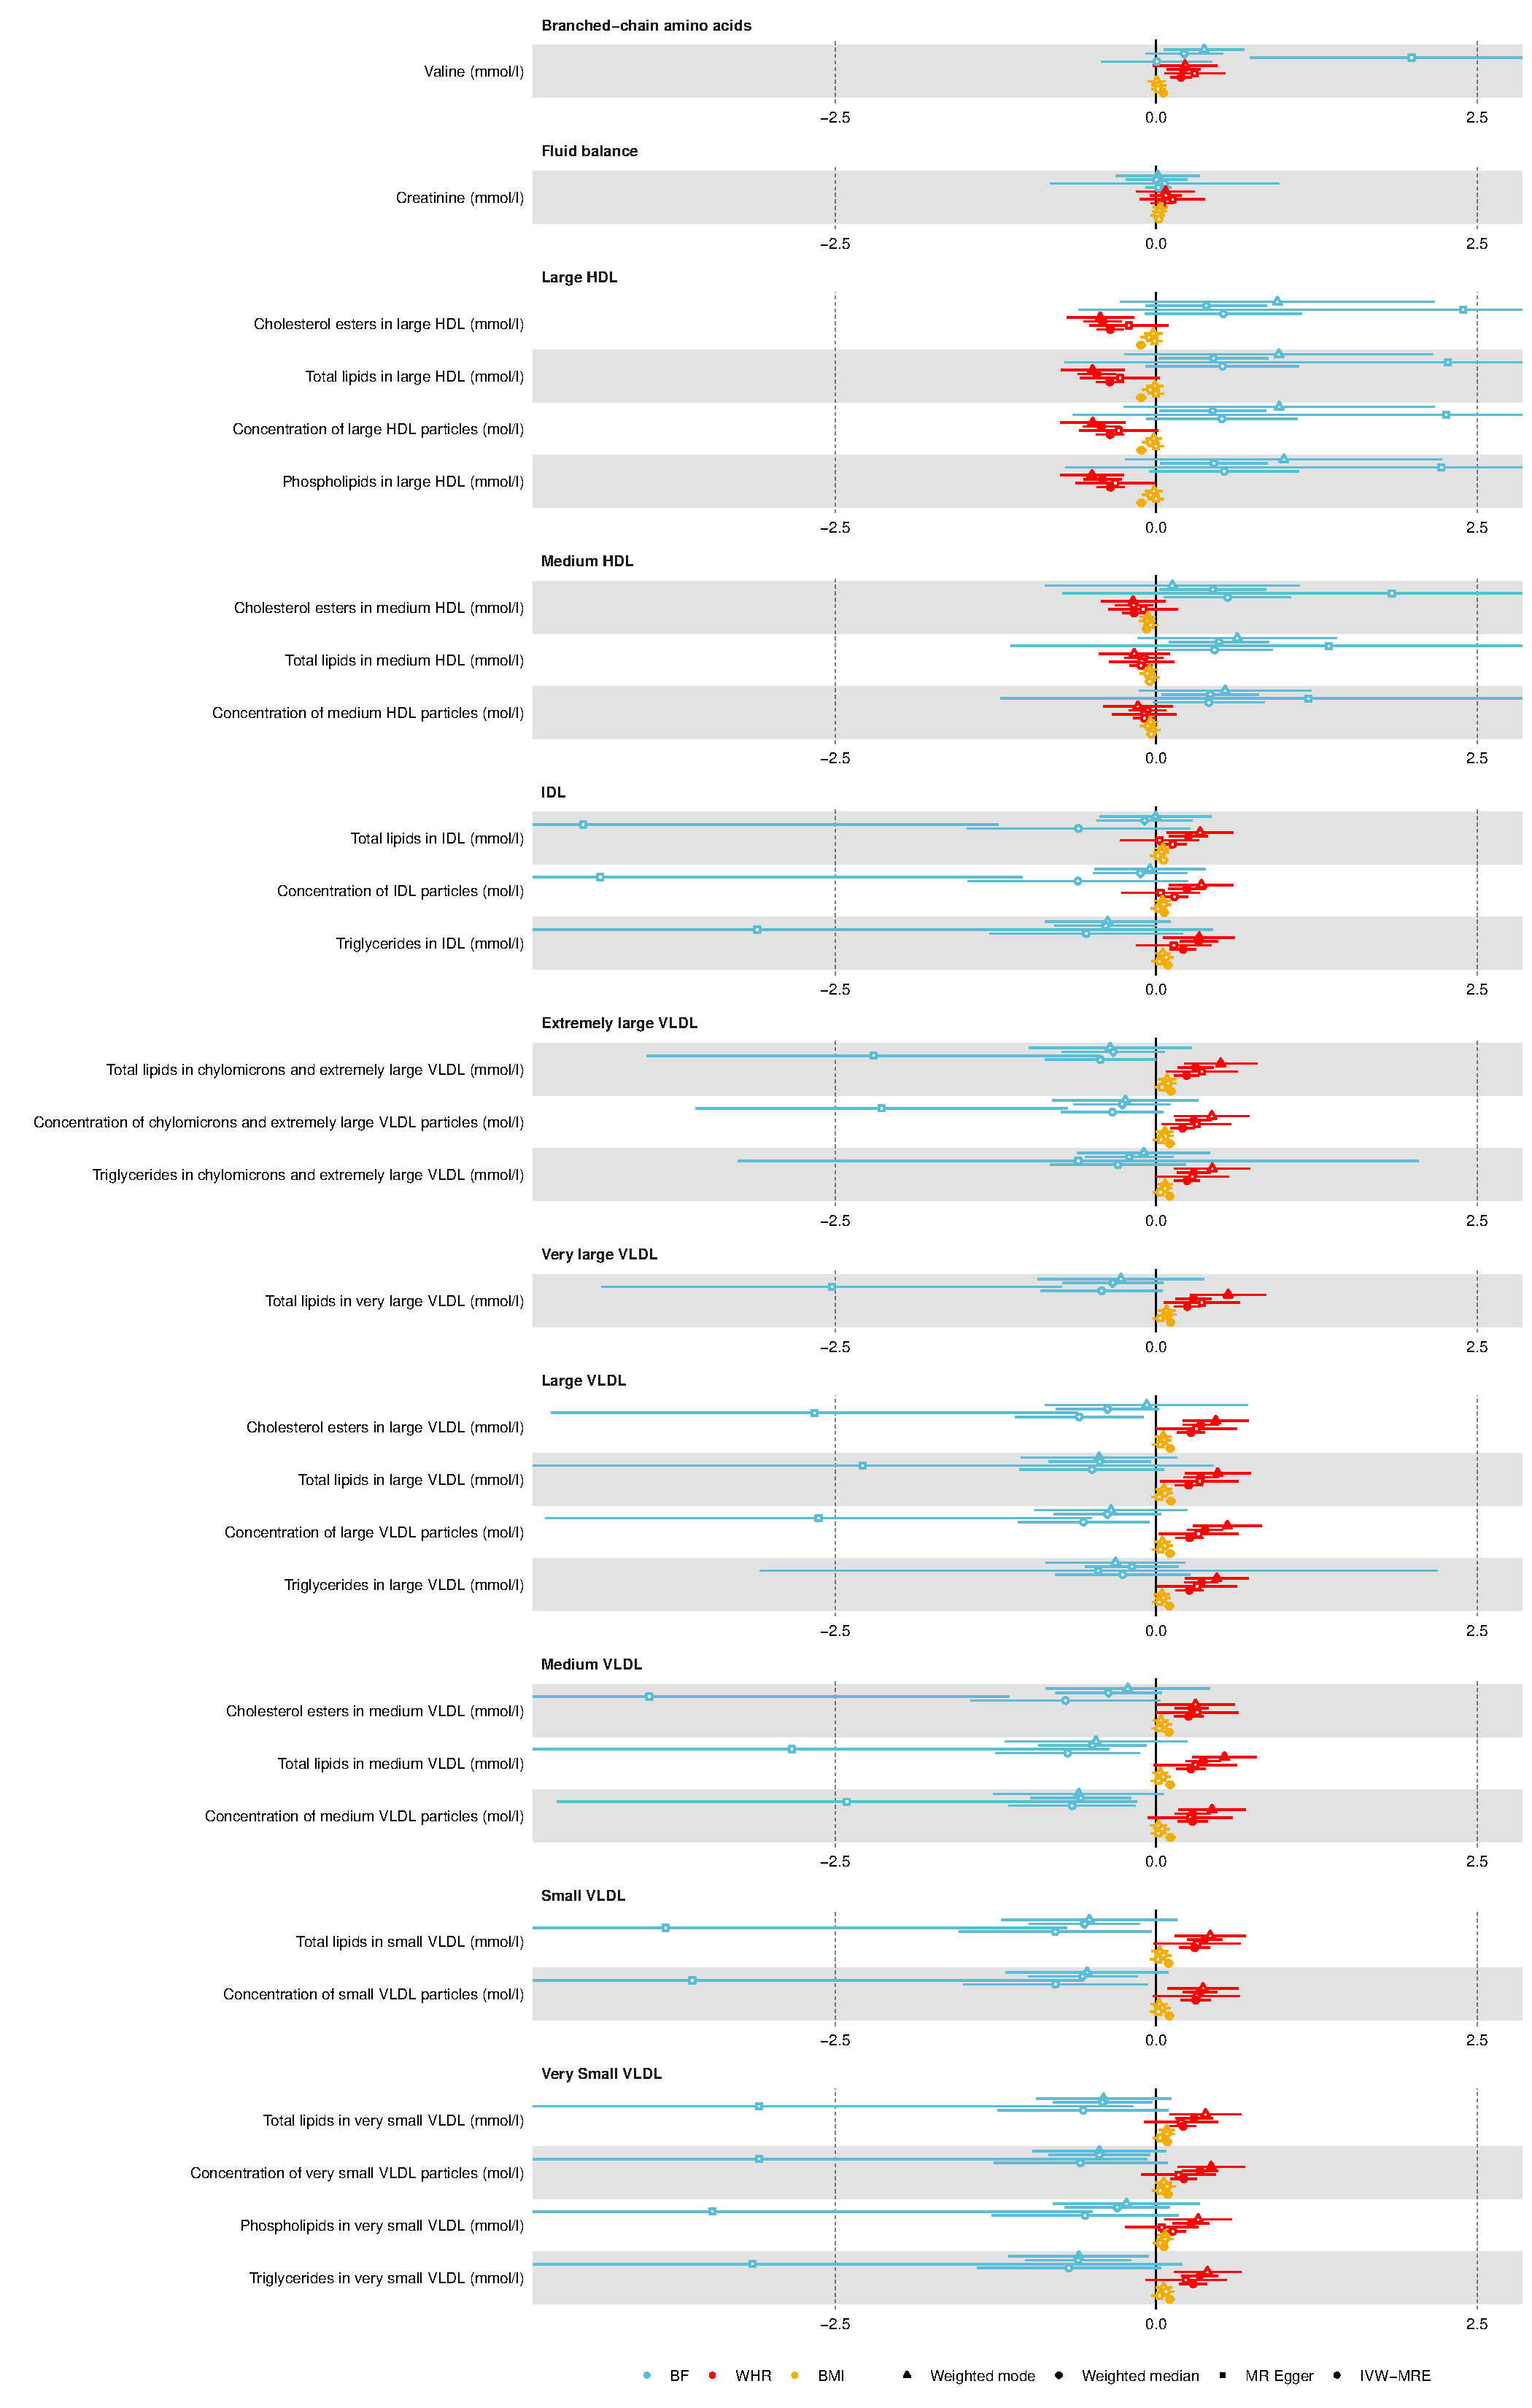
\includegraphics[width=0.9\linewidth]{data/MR/figures/forestplot_kettunen_sensitivity_directional_consistency_combined} \caption[Directionally consistent effects across all two-sample Mendelian randomization models using Kettunen data]{\textbf{Directionally consistent effects across all two-sample Mendelian randomization models using Kettunen data}. Effect estimates and 95\% confidence intervals for metabolites which showed directionally consistent results across the main (IVW-MRE = inverse variance weighted multiplicative random effects) and sensitivity analyses (MR-Egger, weighted median, and weighted mode) within each exposure. Solid points indicate a multiple testing threshold (p-value \textless{} 0.0023) has been reached. BMI = body mass index; WHR = waist hip ratio; BF = body fat percentage. To aid interpretation, the \(X\) axis has been curtailed; confidence intervals for a number of BF estimates exceed the upper and lower \(X\) axis limits. Available on \href{https://github.com/mattlee821/000_thesis/blob/master/index/data/MR/figures/forestplot_kettunen_sensitivity_directional_consistency_combined.pdf}{GitHub}.}\label{fig:MR-figure-forestplot-kettunen-sensitivity-directional-consistency}
\end{figure}



\begin{figure}
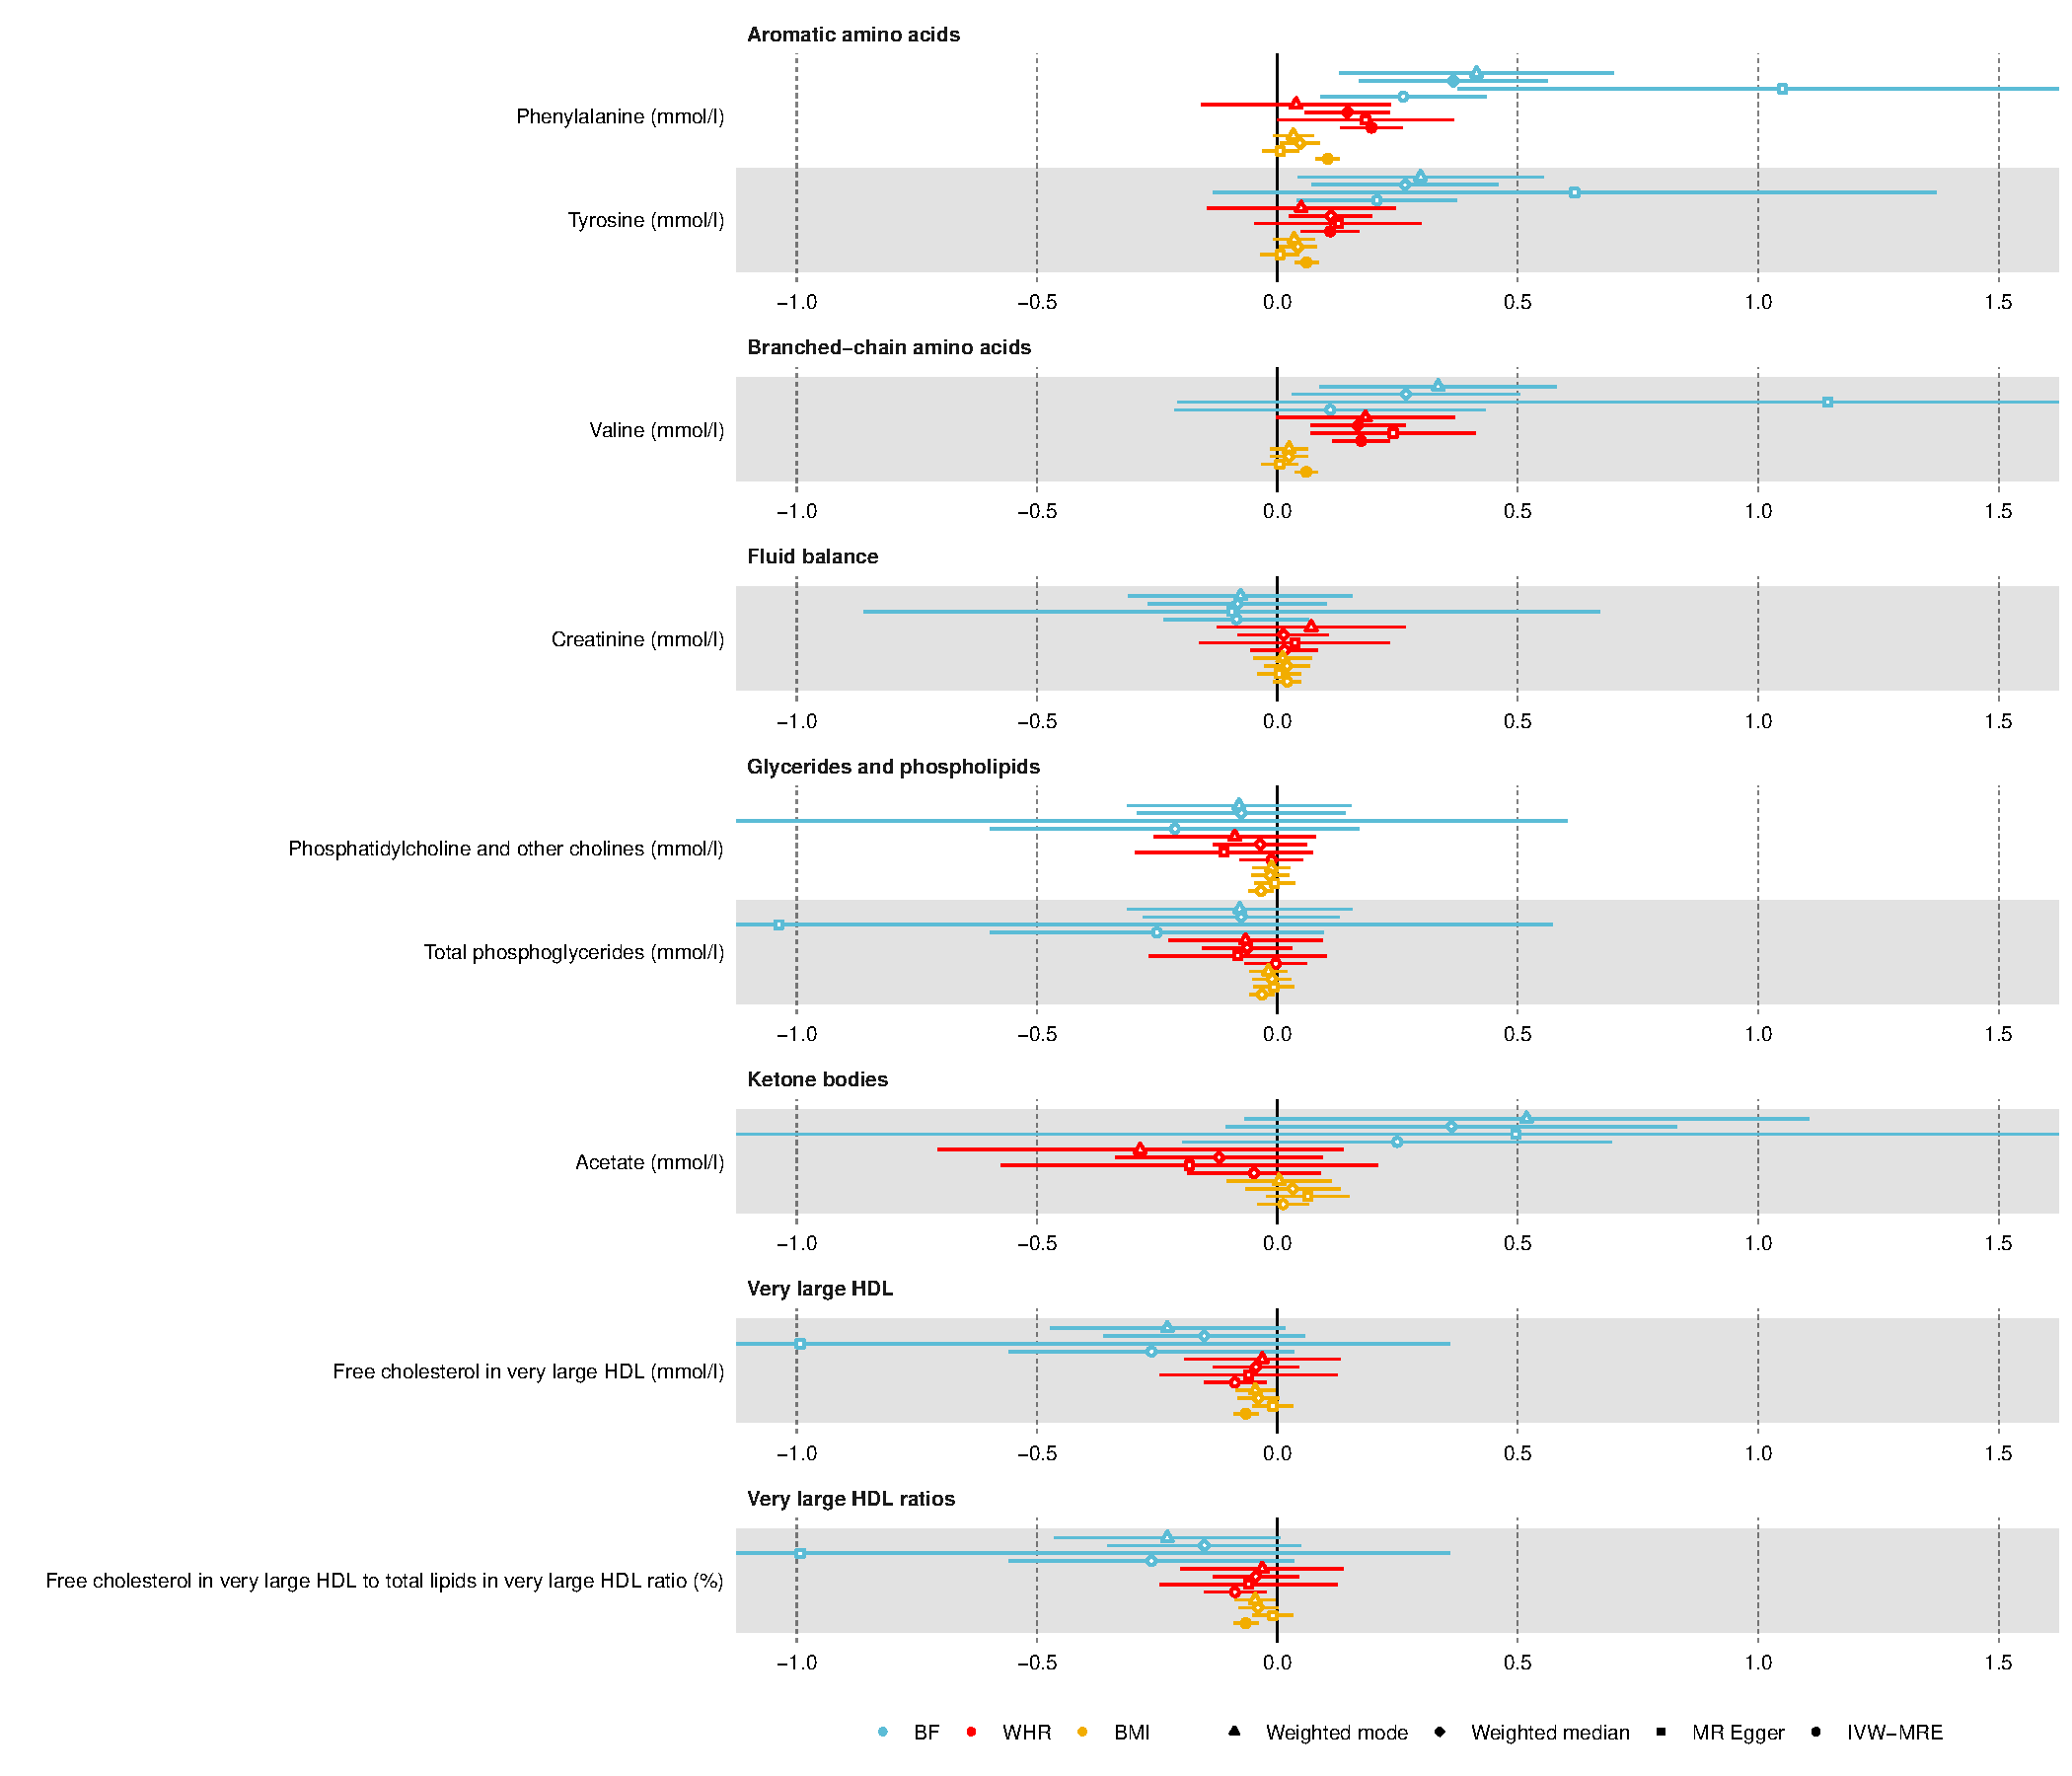
\includegraphics[width=1\linewidth]{data/MR/figures/forestplot_interval_sensitivity_directional_consistency_combined} \caption[Directionally consistent effects across all two-sample Mendelian randomization models using INTERVAL analysis]{\textbf{Directionally consistent effects across all two-sample Mendelian randomization models using INTERVAL data}. Effect estimates and 95\% confidence intervals for metabolites which showed directionally consistent results across the main (IVW-MRE = inverse variance weighted multiplicative random effects) and sensitivity analysis (MR-Egger, weighted median, and weighted mode) within each exposure. Solid points indicate a multiple testing threshold (p-value \textless{} 0.0018) has been reached. BMI = body mass index; WHR = waist hip ratio; BF = body fat percentage. To aid interpretation, the \(X\) axis has been curtailed; confidence intervals for a number of BF estimates exceed the upper and lower \(X\) axis limits. Available on \href{https://github.com/mattlee821/000_thesis/blob/master/index/data/MR/figures/forestplot_interval_sensitivity_directional_consistency_combined.pdf}{GitHub}.}\label{fig:MR-figure-forestplot-interval-sensitivity-directional-consistency}
\end{figure}
The causal direction between the exposure and outcomes were assessed using the Steiger test. In the Kettunen data, a total of 123 tests were performed for each exposure, the causal direction of effect from the exposure to the outcome was ``true'' (i.e., reflecting that a change in the outcome is a consequence of the exposure) for 0 tests for BMI and 5 tests for WHR. In contrast, the causal direction of effect from the exposure to the outcome was ``true'' for 141 tests for BF. When using INTERVAL data, a majority of test directions were found to be ``true.'' A total of 230 tests were performed for each exposure, the causal direction of effect from the exposure to the outcome was ``true'' for 200 tests for BMI, 110 tests for WHR, and 141 tests for BF.

\par

\hypertarget{analysis-using-kettunen-data}{%
\paragraph{Analysis using Kettunen data:}\label{analysis-using-kettunen-data}}

In single-SNP MR using Kettunen data, visual inspection of forest plots showed \(S\) shaped distributions of effect estimates for all tests (Schematic illustration \ref{fig:MR-figure-kettunen-singlesnp-representative-figure}). Effect estimates for some SNPs in the single-SNP MR analysis appeared to be outliers. For example, for the analysis of the association between BMI and glycoproteins, rs4673553 showed a disproportionately larger effect estimate of 22 SD units increase per SD higher BMI (standard error = 0.85; p-value = 5.66 x 10\textsuperscript{-148}) when compared to other SNPs.

\par




\begin{figure}

{\centering 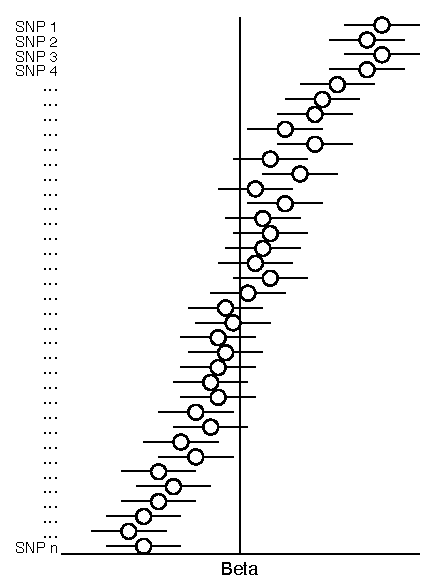
\includegraphics[width=0.5\linewidth]{data/MR/figures/schemeatic_single_snp} 

}

\caption[Schematic illustration: single-SNP Mendelian randomization analysis of the association between adiposity and a metabolite]{\textbf{Schematic illustration: single-SNP Mendelian randomization analysis of the association between adiposity and a metabolite}. In single-SNP Mendelian randomization (MR) analysis, the effect of each SNP on the outcome is investigated. In these analyses, SNP effects are organised from largest to smallest. Here, the figure shows an \(S\) shaped distribution of effects which is representative of the single-SNP MR analyses performed using Kettunen and INTERVAL data.}\label{fig:MR-figure-kettunen-singlesnp-representative-figure}
\end{figure}
To further investigate SNPs with potentially outlying effect estimates, the median effect size across all metabolites for each SNP was investigated. A number of SNPs showed larger median effect sizes across a majority of metabolites. Funnel plots did not however highlight outlying SNPs across all metabolites. Instead, funnel plots were reflective of some SNPs having larger effect estimates more broadly (Representative Figure \ref{fig:MR-figure-kettunen-funnelplot-BMI-representative-figure}). The low number of SNPs used for BF did not result in meaningfully interpretable funnel plots (Representative Figure \ref{fig:MR-figure-kettunen-funnelplot-BF-representative-figure}).

\par




\begin{figure}
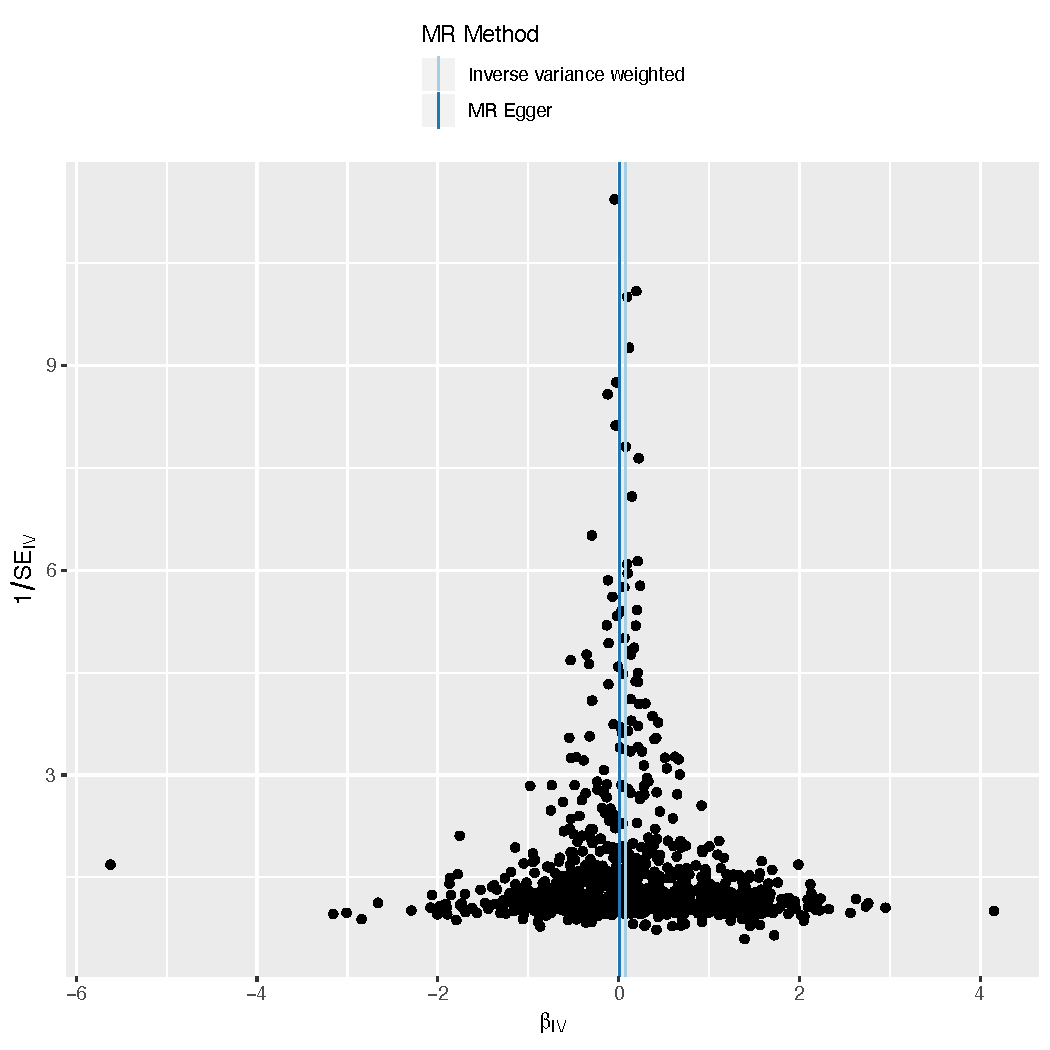
\includegraphics[width=1\linewidth]{data/MR/figures/funnelplot_BMI_representative_figure_kettunen} \caption[Representative figure: funnel plot of effect estimates of the association between body mass index and glycoproteins using Kettunen data]{\textbf{Representative figure: funnel plot of effect estimates of the association between body mass index and glycoproteins using Kettunen data}. Funnel plot shows the effect estimate and standard error from for individual single nucleotide polymorphisms (SNPs). Asymmetry in the funnel may indicate the presence of pleiotropy. The representative figure illustrates a SNP (bottom right) with a larger effect estimate. Effect estimates represent SD unit change in the metabolite per SD unit increase in the exposure.}\label{fig:MR-figure-kettunen-funnelplot-BMI-representative-figure}
\end{figure}



\begin{figure}
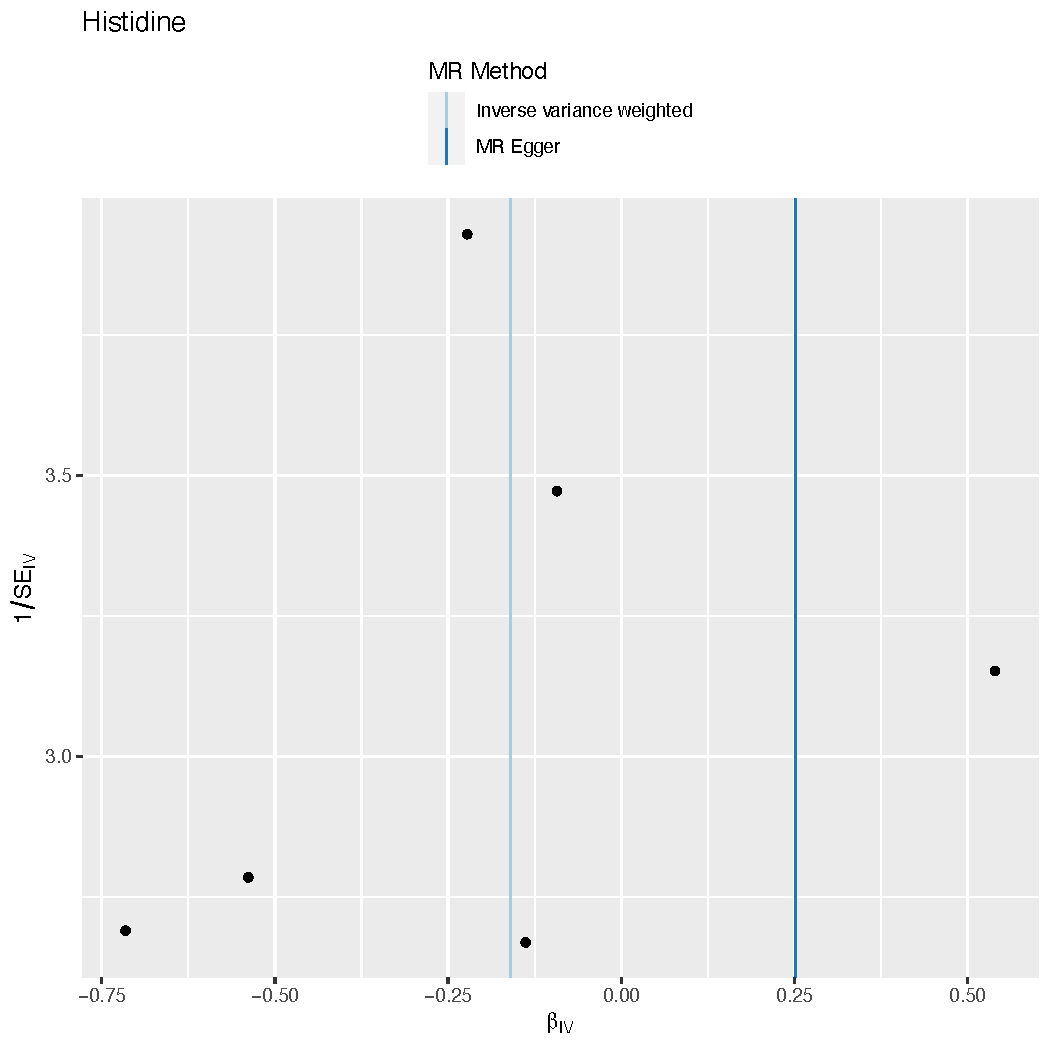
\includegraphics[width=1\linewidth]{data/MR/figures/funnelplot_BF_representative_figure_kettunen} \caption[Representative figure: funnel plot of effect estimates of the association between body fat percentage and histidine using Kettunen data]{\textbf{Representative figure: funnel plot of effect estimates of the association between body fat percentage and histidine using Kettunen data}. Funnel plot shows the effect estimate and standard error from for individual single nucleotide polymorphisms (SNPs). Asymmetry in the funnel may indicate the presence of pleiotropy. The representative figure illustrates a SNP (bottom right) with a larger effect estimate. Effect estimates represent SD unit change in the metabolite per SD unit increase in the exposure.}\label{fig:MR-figure-kettunen-funnelplot-BF-representative-figure}
\end{figure}
Although a number of SNPs showed disproportionately larger effect sizes, in leave-one-out analysis, visual inspection of forest plots showed that no single-SNP altered the direction of effect for any metabolite across exposures. For BF, CIs for one or more SNPs crossed the null for every metabolite tested (Representative Figure \ref{fig:MR-figure-kettunen-leaveoneout-BF-representative-figure}). This was not the case for BMI and WHR, where for many metabolites CIs did not cross the null for any SNPs (Representative Figure \ref{fig:appendix-MR-figure-kettunen-leaveoneout-BMI-representative-figure}).

\par




\begin{figure}
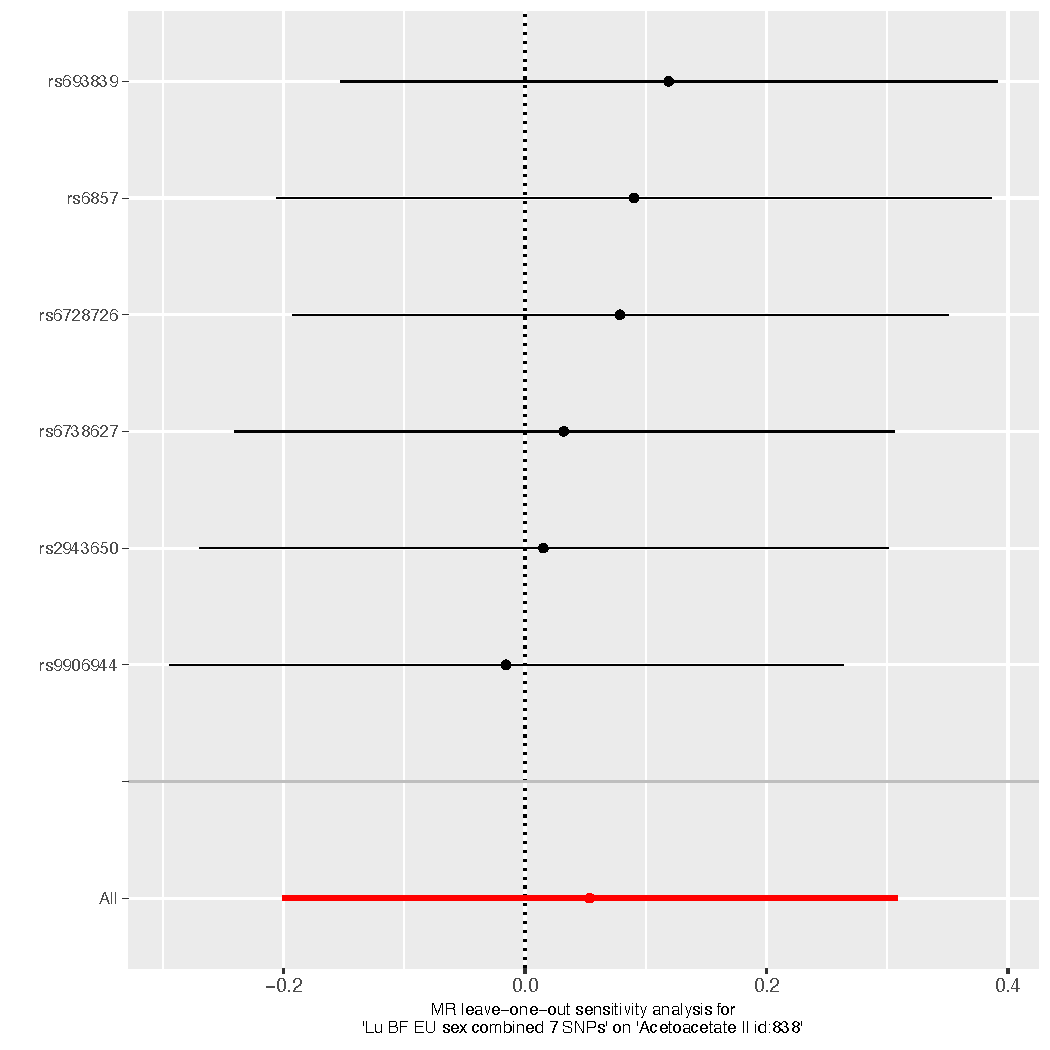
\includegraphics[width=1\linewidth]{data/MR/figures/leaveoneout_BF_representative_figure_kettunen} \caption[Representative figure: leave-one-out MR analysis of the association between body fat percentage and acetoacetate using Kettunen data]{\textbf{Representative figure: leave-one-out MR analysis of the association between body fat percentage and acetoacetate using Kettunen data}. A leave-one-out analysis performs a Mendelian randomization analysis of the exposure and outcome for all single nucleotide polymorphisms (SNPs) excluding a different SNP each time. Forest plot shows the effect estimate and 95\% confidence interval for each SNP exclusion with acetoacetate. Effect estimates represent SD unit change in the metabolite per SD unit increase in the exposure.}\label{fig:MR-figure-kettunen-leaveoneout-BF-representative-figure}
\end{figure}
\hypertarget{analysis-using-interval-data}{%
\paragraph{Analysis using INTERVAL data:}\label{analysis-using-interval-data}}

Broadly speaking, sensitivity analyses using INTERVAL data were similar to that of the sensitivity analyses using the Kettunen data. In single-SNP MR, visual inspection of forest plots showed \(S\) shaped distributions of effect estimates for all tests similar to analyses using the Kettunen data (Representative Figure \ref{fig:appendix-MR-figure-interval-singlesnp-representative-figure}, figure also shows outlier SNP with effect estimate close to -6). As with the Kettunen data, effect estimates for some SNPs in the single-SNP MR analysis were much greater than others.

\par

As with the Kettunen analysis, to investigate whether there were many SNPs with potentially outlying effect estimates, the median effect size across all metabolites for each SNP was investigated. A number of SNPs showed larger median effect sizes across a majority of metabolites. Many of these SNPs had similarly large effect sizes across both the Kettunen and INTERVAL datasets. As an example, for BF, more often than not, rs6857 showed a greater effect estimate than the other 6 SNPs and CIs that did not overlap the null or the 6 other SNPs used as instruments. rs6857 was found in both the Kettunen and INTERVAL data to have a disproportionately larger effect estimate than other SNPs. For BMI and WHR, SNPs with disproportionally larger effect sizes tended to have CIs which overlapped other SNPs. The degree of overlap was minimal however and mostly at the tail-end of the CI.

\par

Funnel plots did not highlight outlying SNPs, but did reflect some SNPs having larger effect estimates across the board (Representative Figure \ref{fig:appendix-MR-figure-interval-funnelplot-BMI-representative-figure}). The low number of SNPs used for BF did not result in meaningfully interpretable funnel plots (Representative Figure \ref{fig:appendix-MR-figure-interval-funnelplot-BF-representative-figure}). In leave-one-out analysis, visual inspection of forest plots showed that no single-SNP altered the direction of effect for any metabolite across exposures. For BF, CIs for one or more SNPs crossed the null for a majority of metabolites tested (Representative Figure \ref{fig:appendix-MR-figure-interval-leaveoneout-BF-representative-figure}). This was not the case for BMI and WHR, where CIs for many metabolite estimates did not cross the null for any SNPs (Representative Figure \ref{fig:appendix-MR-figure-interval-leaveoneout-BMI-representative-figure}).

\par

\hypertarget{additional-analyses-1}{%
\subsubsection{Additional analyses}\label{additional-analyses-1}}

\hypertarget{additional-instruments}{%
\paragraph{Additional instruments}\label{additional-instruments}}

A number of additional SNP lists were used to instrument BMI, WHR, and BF to explore the validity of the instruments used in the main analyses; additional SNP list were obtained for BMI from Yengo et al., (2018)\textsuperscript{\protect\hyperlink{ref-Yengo2018}{53}} using the non-COJO GWAS results (N SNP = 656) and from Locke et al., (2015)\textsuperscript{\protect\hyperlink{ref-Locke2015}{48}} (N SNP = 77), for WHR SNPs were obtained from Shungin et al., (2015)\textsuperscript{\protect\hyperlink{ref-Shungin2015}{49}} (N SNP = 26), for BF the instrument used in the main analysis was used after removing 2 SNPs previously associated with ``favourable adiposity'' and an additional instrument from Hubel et al., (2019)\textsuperscript{\protect\hyperlink{ref-Hubel2019}{55}} (N SNP = 76). Additional SNP lists for BMI and WHR were selected on the basis that they did not contain UK Biobank individuals, which were included in SNP lists for the main analysis. For BF, an additional SNP list which did contain UK Biobank individuals was chosen. For BMI and WHR, additional SNP lists contained fewer SNPs (656 and 77 for BMI and 26 for WHR) than the SNP list used in the main analysis (941 for BMI and 316 for WHR). For BF, the additional SNP list (N SNP = 76) contained more SNPs than the main analysis (N SNP = 7). Each SNP of these additional SNP lists explained a smaller proportion of variance in the exposure compared to the SNP lists used in the main analysis. All details on the additional SNP lists are presented in the Appendix (\ref{appendix-MR-exposures}).

\par

All analyses, including sensitivity analyses, were repeated for these additional SNP lists. Focus here is on the Kettunen data as results were similar for the INTERVAL data, the exception is for the presentation of results from the Steiger directionality test where there were differences. A table of all SNP lists can be found on \href{https://github.com/mattlee821/000_thesis/blob/master/index/data/MR/tables/exposure_SNPs.txt}{GitHub}.

\par

Results from additional instruments for BMI showed broadly larger effect estimates but consistent directions of effect across metabolites (Appendix Figure \ref{fig:appendix-MR-figure-kettunen-circosplot-bmi-additional}) compared to the main analysis. For the BMI SNPs obtained from a non-UK Biobank GWAS, effect estimates had much wider CIs. Spearman's Rho correlation of MR results was highest between the two SNP lists (N SNP = 941 and 656) from Yengo et al., (2018) (Spearmans Rho = 0.98). Correlation between the Locke et al., (2014) SNP list (N SNP = 77) and the COJO SNP list from Yengo et al., (N SNP = 941; Spearmans Rho = 0.9) and the non-COJO SNP list from Yengo et al., (N SNP = 656; Spearmans Rho = 0.93) were also high. For WHR, the pattern of association was similar between both the main analysis (N SNP = 316) and analysis using the additional SNP list from Shungin et al., (2014; N SNP = 26) (Figure \ref{fig:appendix-MR-figure-kettunen-circosplot-whr-additional}) with high correlation between MR results (Spearmans Rho = 0.9). Effect estimates were larger, however CIs were wider and crossed the null more often when using the additional SNP list from Shungin et al., compared to the main analysis.

\par

For BF, there was considerable similarity between the main analysis and the additional analysis when using SNPs from Lu et al., (2016) which did not include two SNPs previously identified as being associated with `favourable adiposity' (Figure \ref{fig:appendix-MR-figure-kettunen-circosplot-bf-additional} and \ref{fig:appendix-MR-figure-interval-circosplot-bf-additional}). More tests reached the multiple testing threshold when using the 5 SNPs from Lu et al., as opposed to the full 7 SNPs, this included associations with apolipoprotein-1, phenylalanine, tyrosine, glucose, and cholesterol esters in very large HDL. For the additional analysis, which used 76 SNPs from Hubel et al., (2016), MR results were considerably smaller and appeared to show conflicting directions of effect with that of the Lu et al., (2016) SNPs (both using 7 and 5 SNPs). CIs were much tighter and two metabolites (phenylalanine and glycoprotein acetyls) reached the multiple testing threshold. Correlation between the two Lu et al., (2016) SNP lists was high (Spearmans Rho = 0.93), however both the 5 (Spearmans Rho = -0.64) and 7 (Spearmans Rho = -0.52) SNP lists from Lu et al., (2016) showed weaker inverse correlations with the SNP list from Hubel et al., (2016).

\par

Steiger directionality tests were variable across analyses (Kettunen vs.~INTERVAL) and instrument lists. Variability between instrument lists is in keeping with the fact that the Steiger test relies on the amount of variance in the exposure that is explained by the genetic instruments to estimate whether a ``true'' causal direction from the exposure to the outcome is identified. When using large instrument lists, as the number of SNPs increases the proportion of variance explained by each individual SNP will decrease. A result of this will be that many SNPs will explain a very low amount of the variance in the exposure.

\par

In the main analysis using BMI with 941 SNPs and the Kettunen data, 0 tests were shown to reflect the ``true'' causal direction of exposure to outcome. However, when using the non-COJO SNPs (N SNP = 656) from the same study, 4 tests were found to reflect the ``true'' causal direction. This increased to 76 tests when using 77 SNPs from Locke et al., (2014)\textsuperscript{\protect\hyperlink{ref-Locke2015}{48}} to instrument BMI. For WHR, a total of 4 tests were shown to reflect a ``true'' causal direction when using the SNP list from Pulit et al., (N SNP = 316). This increased to 102 tests when using the 26 SNP instrument from Shungin et al., (2015)\textsuperscript{\protect\hyperlink{ref-Shungin2015}{49}}. For BF, the 7 SNP instrument resulted in 80 ``true'' tests while the 5 SNP instrument resulted in 76 ``true'' tests. The BF GWAS from Hubel et al., (2019)\textsuperscript{\protect\hyperlink{ref-Hubel2019}{55}} did not have an N available for the summary statistics, instead the total N for the GWAS (155,961) was used. All 123 tests were found to reflect the ``true'' causal direction when using this 76 SNP instrument. When using the INTERVAL data, a different picture was found, with a majority of tests shown to reflect the ``true'' causal direction across all instrument lists. The exception was when instrumenting WHR with 316 SNPs from Pulit et al., (2019)\textsuperscript{\protect\hyperlink{ref-Pulit2019}{54}}, where only 91 tests reflected a ``true'' causal direction for the exposure to the outcome. There was little difference in the number tests that reflected the ``true'' causal direction when instrumenting BMI using 77 SNPs from Locke et al., compared to the 941 SNPs used in the main analysis. As with the Kettunen data, all tests reflected a ``true'' causal direction when instrumenting BF using the 76 SNPs from Hubel et al.,

\par

\hypertarget{clumped-exposures}{%
\paragraph{Clumped exposures}\label{clumped-exposures}}

All of the GWAS used in this Chapter used different thresholds for the identification of independent SNPs. In addition, the main analysis for BMI used COJO identified SNPs in the instrument for BMI. To again test the validity of instruments and ensure associations were not a result of different independence thresholds, all analyses were repeated using instruments that were identified using the same independence thresholds (LD r\textsuperscript{2} \(\geq\) and a 10,000 base window). This clumping process resulted in the removal of the following number of SNPs due to LD (r\textsuperscript{2} \(\geq\) 0.001) with other variants or absence from the LD reference panel: BMI Locke et al., (2014) = 14, BMI Yengo et al., (2018) using COJO SNPs = 583, BMI Yengo et al., (2018) using non-COJO SNPs = 336, WHR Pulit et al., (2018) = 234, WHR Shungin et al., (2014) = 17, BF Hubel et al., (2018) = 4. No SNPs were removed due to clumping for BF from Lu et al., (2016). All SNPs, including whether they were removed due to clumping, are available on \href{https://github.com/mattlee821/000_thesis/blob/master/index/data/MR/tables/exposure_SNPs.txt}{GitHub}.

\par

When using the Kettunen data, correlation for BMI results between the Yengo COJO (Spearmans Rho = 0.97), non-COJO (Spearmans Rho = 0.97), and Locke (Spearmans Rho = 0.98) non-clumped and clumped MR results was high. Similarly, for WHR MR results from non-clumped and clumped analyses correlation was high for the main exposure (Pulit et al., (2018); Spearmans Rho = 0.97) and for the additional exposure (Spearmans Rho = 0.98). For BF, clumping was not possible for the main exposure, however correlation between the non-clumped and clumped SNP list from Hubel et al., (2018) was high (Spearmans Rho = 0.98).

\par

When using the INTERVAL data, correlation for BMI results between the Yengo COJO (Spearmans Rho = 0.96), non-COJO (Spearmans Rho = 0.91), and Locke (Spearmans Rho = 0.93) non-clumped and clumped MR results was high. Similarly, for WHR MR results from non-clumped and clumped analyses correlation was high for the main exposure (Pulit et al., (2018); Spearmans Rho = 0.99) and for the additional exposure (Spearmans Rho = 0.99). For BF, clumping was not possible for the main exposure, however correlation between the non-clumped and clumped SNP list from Hubel et al., (2018) was high (Spearmans Rho = 0.996).

\par

In regards to the Steiger directionality tests when using Kettunen data, clumping generally resulted in a larger number of tests reflecting a ``true'' causal direction from th exposure to the outcome. This increase was largest when using the additional instrument lists as opposed to when using instrument lists used in the main analysis. For example, there was no difference between the BMI 941 SNP instrument and the clumped version (N SNP = 358), but when instrumenting BMI using the 77 SNPs from Locke et al., after clumping (N SNP = 63) the number of ``true'' tests increased from 76 to 79. This was similar for WHR instrumented using the 26 SNPs from Shungin et al., (2015)\textsuperscript{\protect\hyperlink{ref-Shungin2015}{49}}, where 102 and 112 tests were found to reflect the ``true'' causal direction for the non-clumped and clumped (N = 18) SNP lists, respectively. A similar picture was found when using the INTERVAL data, where, although a majority of tests where shown to reflect a ``true'' causal direction, clumping instruments resulted in this number increasing. The exception was when instrumenting WHR with SNPs from Pulit et al., (2019)\textsuperscript{\protect\hyperlink{ref-Pulit2019}{54}}. After clumping (N SNP = 214), the number of tests that reflected the ``true'' causal direction for WHR reduced from 91 to 75.

\par

\hypertarget{post-hoc-analysis}{%
\subsubsection{Post-hoc analysis}\label{post-hoc-analysis}}

To further investigate the difference in directions of effect observed for BMI and WHR, and BF, post-hoc interrogation of results from a single, well characterised, adiposity SNP (rs1558902) was undertaken. Measures of adiposity have been associated with numerous mutations in the \emph{FTO} locus, with studies highlighting major roles in neural signalling of appetite suppression, alongside roles in adipocyte browning\textsuperscript{\protect\hyperlink{ref-Loos2018}{34}}. single-SNP MR analysis using the \emph{FTO} locus (rs1558902; BF beta = 0.051; BMI beta = 0.082) and Kettunen metabolites showed highly consistent results for BF instrumented using the Lu et al., (2016) estimate and BMI instrumented using the Locke et al., (2015) estimate. These results were directionally consistent and differed only in their effect size and standard error which was in line with the difference in the SNP beta for the traits - BMI effect estimates were 62\% larger than BF effect estimates.

\par

\hypertarget{meta-analysis-of-two-sample-mendelian-randomization-results-1}{%
\subsection{Meta-analysis of two-sample Mendelian randomization results}\label{meta-analysis-of-two-sample-mendelian-randomization-results-1}}

In total, 110 metabolites were shared across the Kettunen and INTERVAL metabolite data; a table of results is available on \href{https://github.com/mattlee821/000_thesis/blob/master/index/data/MR/results/meta_analysis_p_results.txt}{GitHub}.. Meta-analysis of p-value was performed using Fisher's method (Equation \eqref{eq:fishers-method}). Across all 3 exposures (330 tests), a total of 120 tests had a positive direction of effect when meta-analysing the Kettunen and INTERVAL data, 91 tests had a negative direction of effect. For BMI a total of 68 tests had a consistent direction of effect across both Kettunen and INTERVAL datatsets, 48 tests had positive directions of effect and 20 tests had negative directions of effect. Similar results were found for WHR (positive = 50; negative = 18). For BF, a larger number of tests had consistent negative directions of effect (N = 53) than positive (N = 22).

\par

Across the 330 tests, a total of 141 tests reached a Bonferroni (0.05/110) multiple testing threshold. Of these, 63 tests had positive directions of effect and 31 tests had negative directions of effect when meta-analysing the Kettunen and INTERVAL data. The remaining 47 tests did not have consistent directions of effect across the Kettunen and INTERVAL MR analyses, e.g., the direction of effect when using the Kettunen data was positive but was negative when using the INTERVAL data. For BMI, 46 tests reached the multiple testing threshold, of which, 30 tests had consistent positive directions of effect and, 16 tests had consistent negative directions of effect. Similar results were found for WHR, where a total of 48 tests reached the multiple testing threshold, with 33 of these having a positive direction of effect across the Kettunen and INTERVAL datasets, and 15 a negative direction of effect. For BF, no metabolites reached the multiple testing threshold.

\par

Across both BMI and WHR, a total of 49 tests reached the multiple testing threshold; 33 tests had a consistent positive direction of effect and 16 tests had a consistent negative direction of effect. As such, a total of 49 metabolites were associated with BMI or WHR in the meta-analysis. Table \ref{tab:MR-table-meta-analysis-sig-direction} gives a list of all 49 metabolites associated with BMI and WHR along with their directions of effect, metabolites are given with their subclass and originally measured units.

\par

\begingroup\fontsize{8}{10}\selectfont
\begin{ThreePartTable}
\begin{TableNotes}[para]
\item Metabolite label and units are given alongside the subclass the metabolites was grouped into and the consistent direction of effect across analyses using Kettunen and INTERVAL data.
\end{TableNotes}
\begin{longtable}[t]{lll}
\caption{\label{tab:MR-table-meta-analysis-sig-direction}Metabolites with a consistent direction of effect between body mass index and waist hip ratio which reached a multiple testing threshold (p-value < 0.00045) in Mendelian randomization meta-analysis}\\
\toprule
Metabolite (units) & Subclass & Direction\\
\midrule
\endfirsthead
\caption[]{\label{tab:MR-table-meta-analysis-sig-direction}Metabolites with a consistent direction of effect between body mass index and waist hip ratio which reached a multiple testing threshold (p-value < 0.00045) in Mendelian randomization meta-analysis \textit{(continued)}}\\
\toprule
Metabolite (units) & Subclass & Direction\\
\midrule
\endhead

\endfoot
\bottomrule
\insertTableNotes
\endlastfoot
\cellcolor{gray!6}{Glutamine (mmol/l)} & \cellcolor{gray!6}{Amino acids} & \cellcolor{gray!6}{-}\\
Phenylalanine (mmol/l) & Aromatic amino acids & +\\
\cellcolor{gray!6}{Tyrosine (mmol/l)} & \cellcolor{gray!6}{Aromatic amino acids} & \cellcolor{gray!6}{+}\\
Isoleucine (mmol/l) & Branched-chain amino acids & +\\
\cellcolor{gray!6}{Leucine (mmol/l)} & \cellcolor{gray!6}{Branched-chain amino acids} & \cellcolor{gray!6}{+}\\
\addlinespace
Valine (mmol/l) & Branched-chain amino acids & +\\
\cellcolor{gray!6}{Apolipoprotein A-I (g/l)} & \cellcolor{gray!6}{Apolipoproteins} & \cellcolor{gray!6}{-}\\
Apolipoprotein B (g/l) & Apolipoproteins & +\\
\cellcolor{gray!6}{Total cholesterol in HDL (mmol/l)} & \cellcolor{gray!6}{Cholesterol} & \cellcolor{gray!6}{-}\\
Monounsaturated fatty acids; 16:1, 18:1 (mmol/l) & Fatty acids & +\\
\addlinespace
\cellcolor{gray!6}{Total fatty acids (mmol/l)} & \cellcolor{gray!6}{Fatty acids} & \cellcolor{gray!6}{+}\\
Serum total triglycerides (mmol/l) & Glycerides and phospholipids & +\\
\cellcolor{gray!6}{Lactate (mmol/l)} & \cellcolor{gray!6}{Glycolysis related metabolites} & \cellcolor{gray!6}{+}\\
Mean diameter for HDL particles (nm) & Lipoprotein particle size & -\\
\cellcolor{gray!6}{Mean diameter for VLDL particles (nm)} & \cellcolor{gray!6}{Lipoprotein particle size} & \cellcolor{gray!6}{+}\\
\addlinespace
Concentration of chylomicrons and extremely large VLDL particles (mol/l) & Extremely large VLDL & +\\
\cellcolor{gray!6}{Phospholipids in chylomicrons and extremely large VLDL (mmol/l)} & \cellcolor{gray!6}{Extremely large VLDL} & \cellcolor{gray!6}{+}\\
Total lipids in chylomicrons and extremely large VLDL (mmol/l) & Extremely large VLDL & +\\
\cellcolor{gray!6}{Triglycerides in IDL (mmol/l)} & \cellcolor{gray!6}{IDL} & \cellcolor{gray!6}{+}\\
Cholesterol esters in large HDL (mmol/l) & Large HDL & -\\
\addlinespace
\cellcolor{gray!6}{Free cholesterol in large HDL (mmol/l)} & \cellcolor{gray!6}{Large HDL} & \cellcolor{gray!6}{-}\\
Total cholesterol in large HDL (mmol/l) & Large HDL & -\\
\cellcolor{gray!6}{Total lipids in large HDL (mmol/l)} & \cellcolor{gray!6}{Large HDL} & \cellcolor{gray!6}{-}\\
Concentration of large VLDL particles (mol/l) & Large VLDL & +\\
\cellcolor{gray!6}{Free cholesterol in large VLDL (mmol/l)} & \cellcolor{gray!6}{Large VLDL} & \cellcolor{gray!6}{+}\\
\addlinespace
Phospholipids in large VLDL (mmol/l) & Large VLDL & +\\
\cellcolor{gray!6}{Total lipids in large VLDL (mmol/l)} & \cellcolor{gray!6}{Large VLDL} & \cellcolor{gray!6}{+}\\
Triglycerides in large VLDL (mmol/l) & Large VLDL & +\\
\cellcolor{gray!6}{Cholesterol esters in medium HDL (mmol/l)} & \cellcolor{gray!6}{Medium HDL} & \cellcolor{gray!6}{-}\\
Free cholesterol in medium HDL (mmol/l) & Medium HDL & -\\
\addlinespace
\cellcolor{gray!6}{Total cholesterol in medium HDL (mmol/l)} & \cellcolor{gray!6}{Medium HDL} & \cellcolor{gray!6}{-}\\
Total lipids in medium HDL (mmol/l) & Medium HDL & -\\
\cellcolor{gray!6}{Free cholesterol in medium VLDL (mmol/l)} & \cellcolor{gray!6}{Medium VLDL} & \cellcolor{gray!6}{+}\\
Total lipids in medium VLDL (mmol/l) & Medium VLDL & +\\
\cellcolor{gray!6}{Triglycerides in medium VLDL (mmol/l)} & \cellcolor{gray!6}{Medium VLDL} & \cellcolor{gray!6}{+}\\
\addlinespace
Total lipids in small HDL (mmol/l) & Small HDL & +\\
\cellcolor{gray!6}{Triglycerides in small HDL (mmol/l)} & \cellcolor{gray!6}{Small HDL} & \cellcolor{gray!6}{+}\\
Total lipids in small VLDL (mmol/l) & Small VLDL & +\\
\cellcolor{gray!6}{Triglycerides in small VLDL (mmol/l)} & \cellcolor{gray!6}{Small VLDL} & \cellcolor{gray!6}{+}\\
Concentration of very large HDL particles (mol/l) & Very large HDL & -\\
\addlinespace
\cellcolor{gray!6}{Free cholesterol in very large HDL (mmol/l)} & \cellcolor{gray!6}{Very large HDL} & \cellcolor{gray!6}{-}\\
Phospholipids in very large HDL (mmol/l) & Very large HDL & -\\
\cellcolor{gray!6}{Total lipids in very large HDL (mmol/l)} & \cellcolor{gray!6}{Very large HDL} & \cellcolor{gray!6}{-}\\
Concentration of very large VLDL particles (mol/l) & Very large VLDL & +\\
\cellcolor{gray!6}{Phospholipids in very large VLDL (mmol/l)} & \cellcolor{gray!6}{Very large VLDL} & \cellcolor{gray!6}{+}\\
\addlinespace
Total lipids in very large VLDL (mmol/l) & Very large VLDL & +\\
\cellcolor{gray!6}{Triglycerides in very large VLDL (mmol/l)} & \cellcolor{gray!6}{Very large VLDL} & \cellcolor{gray!6}{+}\\
Total lipids in very small VLDL (mmol/l) & Very Small VLDL & +\\
\cellcolor{gray!6}{Triglycerides in very small VLDL (mmol/l)} & \cellcolor{gray!6}{Very Small VLDL} & \cellcolor{gray!6}{+}\\*
\end{longtable}
\end{ThreePartTable}
\endgroup{}

\hypertarget{comparison-of-two-sample-mendelian-randomization-and-observational-results-from-chapter-refobservational-1}{%
\subsection{Comparison of two-sample Mendelian randomization and observational results from Chapter \ref{observational}}\label{comparison-of-two-sample-mendelian-randomization-and-observational-results-from-chapter-refobservational-1}}

As all MR analyses performed in this Chapter used summary statistics from GWAS which predominanlty included adults, here, comparison with results from the observational analyses in Chapter \ref{observational} focus on results for adults (i.e., the mothers and fathers). All 49 metabolites identified in the meta-analysis as associated with BMI and WHR were analysed in the observational analysis in Chapter \ref{observational} for adults. In the observational analysis, a multiple testing threshold of 0.05/53 (p-value \textless{} \ensuremath{9\times 10^{-4}}) was used. For the 46 metabolites associated with BMI in the meta-analysis, all showed consistent directions of effect in the observational analysis. Only one metabolite (total lipids in medium HDL, p-value = 0.1) did not reach the multiple testing threshold in the observational analysis for BMI. As such, a total of 45 metabolites were associated with BMI across observational and MR analyses. All 48 metabolites associated with WHR in the meta-analysis had consistent directions of effect in the observational analysis and met the multiple testing threshold in the observational analyses (Figure \ref{fig:MR-figure-associated-metabolites-comparison}).

\par

As no associations reached the multiple testing threshold for BF in the meta-analysis, all metabolites with consistent directions of effect in the meta-analysis for BF (N = 75) were compared for consistent directions of effect with the observational analysis. A total of 74 metabolites directionally consistent in the MR analyses for BF were available in the observational analysis - acetoacetate was not measured in ALSPAC adults. Of these, 4 had consistent negative directions across MR and observational analyses and 7 had consistent positive directions. All 4 metabolites with a consistent negative and consistent positive direction of effect reached the observational multiple testing threshold (p-value \textless{} \ensuremath{9\times 10^{-4}}). The remaining 63 metabolites had inconsistent directions of effect across the observational and MR meta-analysis.

\par

Across the 45, 48 and 9 metabolites associated with BMI, WHR and BF, respectively, which were consistent in both MR and observational analyses, 54 of these metabolites were also associated with at least one measure of adiposity. Figure \ref{fig:MR-figure-associated-metabolites-comparison} shows all 54 adiposity-associated metabolites and the directions of effect in each analysis. Associations were identified as: having consistent directions of effect within exposures across MR and observational analyses and which reached a multiple testing threshold in either the meta-analysis (p-value \(\leq\) \ensuremath{5\times 10^{-4}}; BMI and WHR) and observational analysis (p-value \(\leq\) \ensuremath{9\times 10^{-4}}; BMI and WHR) or just in the observational analysis (BF).

\par

\newpage
\thispagestyle{empty}
\vspace*{-3cm}




\begin{figure}

{\centering 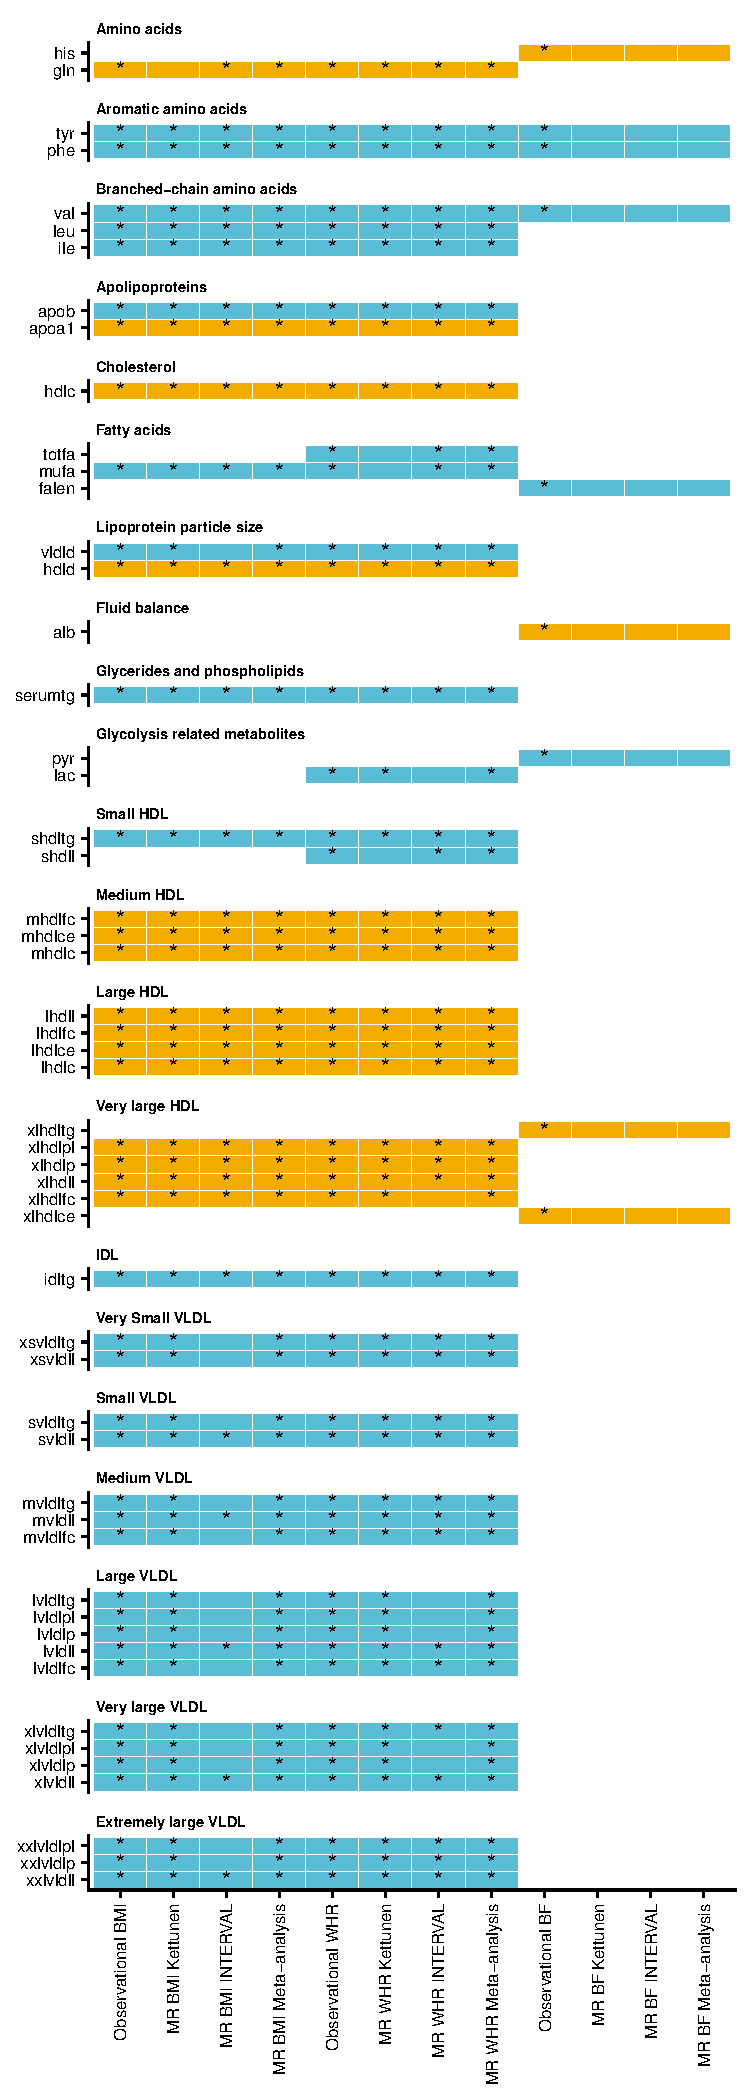
\includegraphics[width=0.95\linewidth]{data/MR/figures/associated_metabolites_comparison} 

}

\caption[Metabolites associated with measures of adiposity in observational and Mendelian randomization meta-analysis]{\textbf{Metabolites associated with measures of adiposity in observational and Mendelian randomization meta-analysis}.}\label{fig:MR-figure-associated-metabolites-comparison}
\end{figure}
\noindent Tile plot shows all metabolites with consistent directions of effect within exposures across observational and Mendelian randomization (MR) meta-analysis and which reached a multiple testing threshold (body mass index (BMI) and waist hip ratio (WHR)) in either the MR meta-analysis and observational analysis (BMI and WHR) or just in the observational analysis (body fat percentage (BF)). Orange tiles indicate a negative direction of effect; blue tiles indicate a positive direction of effect. Multiple testing thresholds: observational = \ensuremath{9\times 10^{-4}}; MR meta-analysis = \ensuremath{5\times 10^{-4}}. Available on \href{https://github.com/mattlee821/000_thesis/blob/master/index/data/MR/figures/associated_metabolites_comparison.pdf}{GitHub}.

\par

\hypertarget{MR-discussion}{%
\section{Discussion}\label{MR-discussion}}

In this chapter, the influence of adiposity on the metabolic profile is demonstrated in an MR framework. The use of MR allowed the interrogation of causality of various measures of adiposity on the metabolic profile, while accounting for limitations in observational analyses (discussed in Chapter \ref{introduction} and \ref{observational}). Data on adiposity measures were available for: BMI from up to 795,624 individuals of European ancestries from GIANT\textsuperscript{\protect\hyperlink{ref-Yengo2018}{53}}, WHR from up to 697,702 individuals of European ancestries from GIANT\textsuperscript{\protect\hyperlink{ref-Pulit2019}{54}}, BF from up to 89,297 individuals European ancestries from Lu et al., (2016)\textsuperscript{\protect\hyperlink{ref-Lu2016}{51}}. Two parallel MR analyses of 123 NMR derived metabolites measured in up-to 24,925 individuals of European ancestries from Kettunen et al., (2016)\textsuperscript{\protect\hyperlink{ref-Kettunen2016}{335}} and 230 NMR derived metabolites measured in up-to 40,905 individuals of European ancestries from INTERVAL (unpublished) were conducted. Meta-analysis of 110 metabolites measured in both the Kettunen and INTERVAL datasets and comparison with observational analyses from Chapter \ref{observational} identified 54 associations between adiposity and metabolite measures that were consistent in direction of effect across MR and observational analyses and passed multiple testing thresholds for one (BF) or both (BMI and WHR) analyses. Positive associations were found for metabolites in VLDL (small, very small, medium, large, and very large), as well as aromatic and branched chain amino acid subclasses. While negative associations were found for HDL (medium, large and very large) subclasses.

\par

In MR analyses, there was evidence for a broad effect of BMI and WHR on the metabolic profile. Both adiposity measures showed positive and negative effects on whole subclasses of metabolites, such as small and very small VLDL, branched chain amino acids (positive), and large and very large HDL (negative). However, there were many effect estimates across the Kettunen and INTERVAL datasets that did not show consistent directions of effect. For example, when using the Kettunen data, positive directions of effect were found for BMI and WHR with very large VLDL. But when using the INTERVAL data, a mix of positive, negative, and null effects were found for BMI and WHR with very large VLDL.

\par

On the whole, MR results revealed WHR to have a broadly larger effect size across metabolites compared to BMI and BF. However, CIs for WHR and BMI mostly overlapped with one another. Evidence for an association between BF and the metabolic profile was weaker. Generally, directions of effect for BF conflicted with those of BMI and WHR. Analyses using BF resulted in larger effect estimates and wider CIs which spanned the null for the majority of metabolites. For example, when using the Kettunen data, BF was negatively associated with metabolites in the medium VLDL subclass, while BMI and WHR were positively associated. When using INTERVAL data, BF was negatively associated with creatinine while BMI and WHR were positively associated. The wide CIs observed for BF and the tighter CIs for BMI are perhaps expected given the variance explained by instruments for each measure of adiposity varied from 0.4\% for BF, 3\% for WHR, and 6\% for BMI.

\par

Consistent directions of effect across all adiposity measures were found for the amino acids tyrosine, phenylalanine, and valine only, which were all positively associated with all measures of adiposity. There were no other metabolites across all three measures of adiposity with a consistent direction of effect. The only other amino acids associated with adiposity were negatively associated with BMI and WHR (glutamine) and by BF (histidine). Results for tyrosine, phenylalanine, and valine are consistent with previous findings, including those by Wurtz et al., (2014)\textsuperscript{\protect\hyperlink{ref-Wurtz2014}{286}}. Although CIs were much wider than results here, Wurtz et al., (2014) found BMI was associated with an increase in glutamine in MR analysis but a decrease in observational analysis. Weak evidence for an increase in histidine was found by Wurtz et al., (2016). Of these associated amino acids, all but glutamine and tyrosine are essential. Increased tyrosine, phenylalanine, and valine have been associated with increased risk of numerous diseases such as colorectal cancer\textsuperscript{\protect\hyperlink{ref-Ritchie2010}{558}--\protect\hyperlink{ref-Brown2016a}{561}}, pancreatic cancer\textsuperscript{\protect\hyperlink{ref-Ritchie2010}{558}}, preeclampsia\textsuperscript{\protect\hyperlink{ref-Bahado-Singh2012}{562},\protect\hyperlink{ref-Bahado-Singh2014}{563}}, irritable bowel syndrome\textsuperscript{\protect\hyperlink{ref-LeGall2011}{564},\protect\hyperlink{ref-Hong2011}{565}}, and crohns and ulcerative colitis\textsuperscript{\protect\hyperlink{ref-Bjerrum2015}{566}}. Reductions in glutamine and histidine meanwhile have been associated with colorectal\textsuperscript{\protect\hyperlink{ref-Ni2014}{559},\protect\hyperlink{ref-Lin2016}{560},\protect\hyperlink{ref-Ikeda2012}{567}} and pancreatic cancer\textsuperscript{\protect\hyperlink{ref-Ikeda2012}{567},\protect\hyperlink{ref-Zhang2012}{568}}. There is some conflicting evidence however, with higher histidine levels also found to be associated with colorectal cancer\textsuperscript{\protect\hyperlink{ref-Goedert2014}{569}}. A recent prospective analysis found associations between 12 metabolites and increased risk of endometrial cancer, including, tyrosine, phenylalanine, leucine, and isoleucine. However, after adjusting for BMI only the association between glycine and serine with endometrial cancer remained\textsuperscript{\protect\hyperlink{ref-Dossus2021}{570}}. Given many of these metabolites were associated with adiposity, it is possible they may be intermediates in the adiposity relationship with endometrial cancer, among other outcomes.

\par

For BMI and WHR, directions of effect were the same across all associated metabolites. BMI and WHR were both associated with reductions of metabolites in medium HDL, large HDL, and very large HDL subclasses, as well as reductions in apolipoprotein A-1, mean diameter for HDL particles, and total cholesterol in HDL. In addition, BMI and WHR were both associated with increases in numerous LDL subclasses (e.g., IDL and very small VLDL) as well as apolipoprotein B. These results are supported by the underlying relationship between HDL and LDL metabolites as well as similar results in numerous MR\textsuperscript{\protect\hyperlink{ref-Wurtz2014}{286},\protect\hyperlink{ref-Bull2020}{415},\protect\hyperlink{ref-Bell2021a}{544}} and observational\textsuperscript{\protect\hyperlink{ref-Wurtz2014}{286},\protect\hyperlink{ref-Cirulli2019}{287},\protect\hyperlink{ref-Moore2014}{345},\protect\hyperlink{ref-SantosFerreira2017}{386}--\protect\hyperlink{ref-Rangel-Huerta2019}{395}} analyses. Apolipoprotein A1 is the major component of HDL particles and enables uptake of lipids by HDL from cells. HDL particles primarily transport lipids away from the cells, in what is known as reverse cholesterol transport. These lipids end up at the liver where they are recycled and excreted\textsuperscript{\protect\hyperlink{ref-Feingold2000}{534},\protect\hyperlink{ref-Marz2017}{535}}. Apolipoprotein B on the other hand is the major component of VLDL, IDL, and LDL particles, enabling lipid uptake, and thus increased transport of lipids around the body\textsuperscript{\protect\hyperlink{ref-Feingold2000}{534},\protect\hyperlink{ref-Venugopal2021}{571}}.

\par

Observational studies have highlighted increased HDL to be associated with a protective effect on cardiovascular disease (CVD)\textsuperscript{\protect\hyperlink{ref-Kosmas2018}{572}} while increased LDL is shown to increase CVD risk\textsuperscript{\protect\hyperlink{ref-Ference2017}{573}}. MR studies support observational results for LDL\textsuperscript{\protect\hyperlink{ref-Ference2017}{573}}, but are conflicting for HDLs protective effect\textsuperscript{\protect\hyperlink{ref-White2016}{574}}. Randomised controlled trials have also not found strong evidence for an effect of HDL lowering drugs on CVD risk\textsuperscript{\protect\hyperlink{ref-Holmes2017}{575}}. Some focus has been given to a measure of HDLs contribution to reverse cholesterol transport, HDL cholesterol efflux capacity (HDL-CEC), which has been shown to be protective for CVD\textsuperscript{\protect\hyperlink{ref-Rohatgi2014}{576},\protect\hyperlink{ref-Kuusisto2019}{577}}. Estimation of HDL-CEC however was not available in the current analyses. There are also associations between reduced HDL and many cancers, however there is some evidence to suggest this may be bi-directional\textsuperscript{\protect\hyperlink{ref-Pirro2018}{578}}. Recent work has suggested that increased HDL does not confer a protective benefit on mortality\textsuperscript{\protect\hyperlink{ref-Ala-Korpela2021}{579}}, and instead there is evidence that apolipoprotein B may underlie the association between many lipids and diseases such as coronary heart disease (CHD)\textsuperscript{\protect\hyperlink{ref-Richardson2020}{580}}. Apolipoprotein B and its associated lipids, such as VLDLs, may therefore be potential intermediates in disease associations.

\par

There was considerable heterogeneity in the effect estimates derived from the different genetic instruments used in the main analysis. In addition, directional consistency across the main (IVW-MRE) and sensitivity analyses (MR-Egger, weighted median, and weighted mode) was inconsistent for a majority of exposure-outcome pairs for BMI and BF analyses using both the Kettunen and INTERVAL datasets. That is, for a consistent direction to be recorded for one exposure-outcome pair (e.g., the association of BMI and phenylalanine) the direction of effect for all 4 models must be in the same direction. For WHR, a majority (\textasciitilde70\%-80\%) of exposure-outcome pairs across the main and sensitivity analyses had consistent directions of effect. Broadly, inconsistency in the directions of effect was driven by effect estimates from MR-Egger tests. In single-SNP MR analysis, a number of SNPs showed disproportionately larger effect estimates across many metabolites. However, ``leave-one-out'' analysis did not highlight any individual SNP driving the effect for any one metabolite. The inconsistent directions of effect across models for BMI and BF may therefore be a result of reduced power in MR-Egger tests compared to the other models, heterogeneity of the instruments, and the presence of pleiotropy.

\par

Steiger directionality tests can provide an estimate as to whether the ``true'' causal direction of an MR analysis has been tested. That is, if we perform the analysis of exposure \(A\) on outcome \(B\) and our hypothesis is that \(A\) causes \(B\), the Steiger test will estimate whether this direction (\(A\) to \(B\)) is ``true''. The test relies on using effect size to estimate variance explained in the exposure and outcome. Results from the Steiger test varied across analyses using Kettunen and INTERVAL data. For analyses using the Kettunen data, a majority of tests did not reflect the ``true'' causal direction, which were primarily driven by analyses with BMI and WHR. When using the INTERVAL data, a majority of tests reflected the ``true'' causal direction. As the majority of analyses using additional instrument lists for BMI and WHR, for which all instruments were included in the larger main analysis instruments, reflected a ``true'' causal direction, these results should be interpreted with caution. Assuming that the causal direction is from adiposity to metabolites, if the variance explained by SNPs in BMI is small it should be smaller in the outcomes except in the presence of pleiotropy or if the power in the outcome GWAS is greater than in the exposure GWAS. Given the large sample size for the exposure GWASs (\textgreater{} 400,000) compared to the outcome GWASs (maximum \textasciitilde40,000) it is likely pleiotropy is a greater issue here than power. For BF, results of the Steiger test are likely more complex, given that many tests found to be ``true'' when using the Kettunen data were also found to be ``true'' when using the INTERVAL data even though directions of effect were different. It is unclear why there is a difference here, but it may be due to the instrumentation of BF, which, unlike BMI and WHR, has been linked with `favourable adiposity'. It may also be reflective of differences in the underlying populations used in the outcome GWAS. Though both are of European ancestries, the Kettunen at al., GWAS consisted mostly of individuals from Scandinavia (predominantly Finland), while the INTERVAL GWAS consisted mostly of individuals from the United Kingdom. There is evidence of population structure across Europe\textsuperscript{\protect\hyperlink{ref-Salmela2008}{581}} and genetic differences between Finnish and British populations\textsuperscript{\protect\hyperlink{ref-Chheda2017}{582}}.

\par

\hypertarget{strengths-and-limitations-1}{%
\subsection{Strengths and limitations}\label{strengths-and-limitations-1}}

The key strengths of this work are the (i) complimentary analyses with Chapter \ref{observational}, (ii) complimentary measures of adiposity to comprehensively examine the association between adiposity and metabolites, (iii) the use of many different GWAS to investigate instrumentation, (iv) and the replication of adiposity-associated metabolites across independent datasets. Metabolomic data from Kettunen et al., and INTERVAL used the same metabolomic platform used for ALSPAC in Chapter \ref{observational}. Though the platform is predominantly lipid based, data were available across all three datasets for many non-lipid metabolites such as amino acids, inflammation markers, and glycolysis related metabolites. Use of complimentary measures of adiposity here highlighted broadly larger effects for WHR and inconsistent results between BMI and WHR, and BF unlike in observational analyses. However, consistent directions of effect across all three exposures were found for a small number of metabolites, such as phenylalanine and tyrosine. Follow-up analysis, including the use of alternative instrument lists for each adiposity exposure, suggested instrumentation of BF is perhaps more complex than instrumenting BMI and WHR. Additionally, replication and meta-analysis using two independent datasets (Kettunen et al., and INTERVAL) strengthens evidence for an association. Importantly, triangulation of evidence across observational and MR analyses, which have different sources of bias, further strengthens evidence for an association between adiposity and 54 metabolites.

\par

MR analyses are subject to a number of assumptions, the main three being: (i) the instrumental variable (\(Z\)) is robustly associated with the exposure (\(X\)), (ii) there are no common causes of the instrument and outcome (\(Y\)); and (iii) there is no independent association between the instrumental variable and the outcome other than through the exposure. In this work, instruments were obtained from large well-powered GWAS, and the F-statistics for each instrument was above a nominal threshold of 10 meaning the first assumption was likely met. In regards the other two assumptions, formal testing is not possible. However, sensitivity analyses can provide an indication of pleiotropy and, though not exhaustive, sensitivity analyses conducted here were concordant with the main analysis, suggesting that there is no large impact of pleiotropy on these results. However, as discussed, there may be additional cautions to be taken with the BF analysis, where instrumentation is currently likely to be inadequate.

\par

An additional consideration with regards to instrumentation is the possibility that SNPs associated with adiposity traits may also be associated directly with metabolites or metabolic pathways. The Steiger directionality test can be used to test whether the ``true'' causal direction is the one under investigation, i.e.~the effect of adiposity measures on metabolites. There are a number of limitations associated with the Steiger test\textsuperscript{\protect\hyperlink{ref-Hemani2017}{556}}, one of which is that it assumes that there are no pleiotropic effects. The Steiger test uses effect size to estimate the variance explained by each SNP in the exposure and outcome respectively. In a well powered study, as more SNPs are included in an instrument there is a greater chance of including SNPs with small effect sizes for the exposure. Although the additional analyses for BMI and WHR, which used smaller SNP lists compared to the main analysis, were found to reflect the ``true'' causal direction more often than the main analysis, the high correlation between the two analyses both in terms of effect size and direction of effect would suggest that any associations between the SNPs used in the main analysis with the outcomes did not drastically affect results. This does not fully address the potential for direct associations between exposure-related SNPs and the outcome however, and future work should look at exploring the genetic correlation between the traits.

\par

MR relies upon the use of an instrument to model the effect of an exposure on an outcome. This relationship is dependent upon the genetic architecture of the instruments and the traits under investigation, as well as power (predominantly sample size of the data from which the estimates of the association between the instrument and outcome are derived), both of which influence the utility of the various MR methods. The first MR assumption, that the instrument is robustly associated with the exposure, is generally measured via an F-statistic, for which an arbitrary threshold of \textgreater{} 10 denotes a strong instrument. All of the instruments used here exceeded this threshold. In addition, the variance explained in an exposure by genetic variants can indicate the power afforded in the MR analysis; the variance explained in exposures used in the main analysis varied from 6\% for BMI, to 3\% for WHR, and \textasciitilde0.4\% for BF. The considerably lower variance explained for BF may have impacted on results as there would be less power in the MR analyses which may result in wider CIs; when using additional instrument lists for BMI and WHR, which explained a lesser percentage of variance, CIs became wider. Winners curse is unlikely given summary statistics used here are well powered and underwent replication by the authors of the original GWAS publications.

\par

The consistent directions of effect observed across BMI and WHR measures adds weight to their associations with metabolites. For BF, conflicting directions of effect were observed when comparing to BMI and WHR. However, CIs were wider and, although they spanned the null, included the estimates and CIs for BMI and WHR in a majority of cases. There was considerable difference in the sample sizes used in the GWAS for BMI, WHR, and BF. In addition, whereas BMI and WHR were measured in only one way for their respective GWAS, the BF GWAS included measures of BF from DXA and impedance devices. Though, as shown in Chapter \ref{observational}, DXA and impedance measures of BF are highly correlated, the additional analysis for BF which used only impedance measures in the GWAS showed much greater directional consistency with BMI and WHR and also included a number of metabolites which reached the multiple testing threshold. Given the highly correlated nature of the exposures, and the consistency in observational estimates with metabolites, results for BF here appear counter-intuitive. Additional analyses failed to appropriately account for the differences in results and further investigation of instrumentation is warranted.

\par

The instrumentation approach used in the main analysis followed that used by the majority of analyses reviewed in Chapter \ref{systematic-review}. That is, instruments were obtained directly from the most recently published GWAS with the largest sample size. As GWAS sample sizes increase, so does the likelihood of sample overlap, which can bias estimates towards the confounded observational effect in the presence of weak instruments. Additionally, there is the concern of population structure within all GWAS, both large\textsuperscript{\protect\hyperlink{ref-Haworth2019}{366},\protect\hyperlink{ref-Lawson2020}{548}--\protect\hyperlink{ref-Sanderson2021}{550}} and small\textsuperscript{\protect\hyperlink{ref-Sohail2019}{373}}, which, if not accounted for appropriately, can lead to violation of the independence assumption and bias estimates towards the confounded observational estimate. Additional analyses, which used a number of different instrumentation practices, including using GWAS which did not include UK Biobank participants and using a standardised clumping strategy, aimed to reduce the impact of population structure that has been demonstrated in UK Biobank and the criteria of defining independence of SNPs was the same within and between exposure instrument lists. Additional BMI and WHR exposures, which did not include UK Biobank participants, showed consistent results with the main analysis. For BF, there was little difference between the main analysis and the additional analysis which used 5 SNPs from Lu et al., (2015)\textsuperscript{\protect\hyperlink{ref-Lu2015}{188}} having removed two SNPs that likely have different biological function. However, there was considerable difference in directions of effect when using the additional SNP list from Hubel et al., (2019)\textsuperscript{\protect\hyperlink{ref-Hubel2019}{55}}.

\par

There is clearly complexity in the choice of instrument, especially with complex traits such as adiposity. This complexity is perhaps well demonstrated through the BF analysis. For BF, there was considerable difference in effect estimates compared to the BMI and WHR results, with a large proportion of estimates in the opposite direction to those of BMI and WHR. This is counter-intuitive given the strong correlation between BMI, WHR, and BF, and the consistent results obtained in observational analyses in Chapter \ref{observational} between BMI, WHR, and BF. Removal of two SNPs previously associated with `favourable adiposity'\textsuperscript{\protect\hyperlink{ref-Yaghootkar2014}{47},\protect\hyperlink{ref-Yaghootkar2016}{557}} resulted in a global tightening of CIs and a number of effect estimates changing direction to be more consistent with BMI and WHR. A number of these effects subsequently reached the multiple testing threshold. However, the majority of MR results remained opposite to that of BMI and WHR. In post-hoc analysis investigating the directional inconsistency between BMI and WHR and BF, effect estimates from a single-SNP MR using rs1558902 to instrument BMI and BF resulted in highly consistent directions of effect across all Kettunen metabolites (data not shown). Results differed only in their effect size and standard error. This difference was in line with the difference in the SNP beta from the BMI (0.082) and BF (0.051) GWAS. Leave-one-out analysis for BF instrumented using the 7 genetic variants identified in Lu et al., (2016) did not indicate a single-SNP that could be driving a pleiotropic association. However, median effect estimates for rs6857 (rs6857 is associated with \emph{NECTIN2} and has previously been associated with a number of diseases including Alzheimer's disease\textsuperscript{\protect\hyperlink{ref-Ferrari2017}{583}}) were much larger than those for other SNPs, both with and without exclusion of the two `favourable adiposity' SNPs. In many cases, rs6857 did not span the null. It is possible that tests for pleiotropy were underpowered however. The unexpected results for BF instrumented using the Lu et al., (2016) genetic variants may be due to a variety of reasons, not least measurement error, sample size differences between BF (up-to 89,297), BMI (up-to 795,624), and WHR (up-to 697,702), and the variance explained by the respective instruments: BF = 0.416\%, WHR = 3\%, BMI = 6\%. The complexity of instrumentation is discussed further in the discussion Chapter \ref{discussion} as this is also relevant to Chapter \ref{mediation}.

\par

As discussed in the limitations section of Chapter \ref{observational}, there is no standardised approach, nor a gold standard, for performing metabolomics quality control. In Chapter \ref{observational}, quality control, including outlier detection and removal, was performed using the \texttt{metaboprep} \texttt{R} package. Metabolite data here however were from summary statistics, the data that went into these GWAS will have undergone different quality control procedures for the metabolomics data. Transformations and inclusion of covariables were not consistent across the Kettunen et al., and INTERVAL metabolomic data. Kettunen et al., did not transform metabolites prior to inverse rank normally transforming residuals, whereas data from INTERVAL were log transformed prior to inverse rank normal transformation. It was therefore not appropriate to meta-analyse effect estimates. Future work should look to use a standardised method for pre-analysis quality control of metabolomics data, such as \texttt{metaboprep}, while ensuring study-specific adjustments are made where appropriate. On the latter point, a centralised approach to analysis of metabolomics data, such as that being employed by the Consortium of Metabolomics Studies\textsuperscript{\protect\hyperlink{ref-Temprosa2021}{584}}, will allow for more efficient comparisons and meta-analyses of studies.

\par

\hypertarget{conclusion-2}{%
\subsection{Conclusion}\label{conclusion-2}}

Adiposity exerts a systemic impact on the metabolome, which is consistent across multiple measures of adiposity (namely, BMI and WHR). Results here highlight a number of metabolites associated with adiposity which have consistent directions of effect and effect sizes with previous MR analyses\textsuperscript{\protect\hyperlink{ref-Wurtz2014}{286},\protect\hyperlink{ref-Bull2020}{415}}. Many results found for BMI and WHR were consistent across two independent datasets and, whilst there is a systemic impact of adiposity on the metabolome, there were 54 analyses that were strongest across multiple study designs, reaching a multiple testing threshold in both observational and MR analyses. Of these 54 unique metabolites, 45 metabolites were associated with BMI, 48 were associated with WHR, and 9 were associated with BF. Some of these metabolites have previously been shown to be associated with adiposity-related diseases such as colorectal\textsuperscript{\protect\hyperlink{ref-Bull2020}{415}} and endometrial cancer\textsuperscript{\protect\hyperlink{ref-Kliemann2021}{585}}, meaning that they could play an intermediary role in these relationships. However, this possible intermediary role of adiposity-associated metabolites on various health outcomes are yet to be explored systematically, especially in an MR context. Although adiposity instrumentation has been well established, and shown here to give consistent results across many different instrument lists and exposures, results for the main BF analysis presented here remain inconsistent with BMI and WHR. Therefore, proper consideration of the appropriate use of genetic variants when compiling instruments for use in MR analyses is required, especially when instrumenting complex traits such as those presented here. By extension, instrumentation is of particular importance when investigating associations between adiposity-associated metabolites identified here and diseases identified in Chapter \ref{systematic-review}. In Chapter \ref{mediation}, investigation of the intermediary role of these adiposity-related metabolites and an exemplar outcome perturbed by adiposity as identified in meta-analysis in Chapter \ref{systematic-review}, endometrial cancer, will be explored.

\par

\newpage

\hypertarget{mediation}{%
\chapter{Associations between adiposity-associated metabolites and endometrial cancer: Mendelian randomization analysis}\label{mediation}}

\hypertarget{chapter-summary-5}{%
\section*{Chapter summary}\label{chapter-summary-5}}
\addcontentsline{toc}{section}{Chapter summary}

This Chapter pulls together information from previous chapters to investigate the effects of adiposity-associated metabolites on endometrial cancer. In Chapter \ref{systematic-review}, a systematic review and meta-analysis showed that adiposity was likely causally implicated in 13 diseases as well as other traits including systolic blood pressure and fasting glucose. Of these, endometrial cancer, with which body mass index (BMI) was strongly related (OR = 1.57; 95\% CI = 1.11 -- 2.22; p-value = 0.01), was selected for further investigation in this Chapter. Here, two-sample Mendelian randomization (MR) was used to estimate the association between adiposity (BMI, waist-hip ratio (WHR), and body fat percentage (BF)) and endometrial cancer, extending analyses presented in Chapter \ref{systematic-review} by including a more comprehensive set of adiposity measures and increasing the sample sizes of data sources. Two-sample univariable MR was performed to estimate the effect of adiposity-associated metabolites, characterised in analyses undertaken in chapters \ref{observational} and \ref{MR}, and endometrial cancer. To understand whether metabolites, for which there was evidence for an association with endometrial cancer, may play an intermediary role in the relationship between adiposity and endometrial cancer, the largest causal analysis (including multivariable MR; MVMR) to date was performed.

\par

\newpage

\hypertarget{mediation-introduction}{%
\section{Introduction}\label{mediation-introduction}}

In chapters \ref{introduction} and \ref{systematic-review}, I showed that the number of adiposity-associated diseases is high, consistent with adiposity being a global health concern\textsuperscript{\protect\hyperlink{ref-WorldHealthOrganisation2018}{2},\protect\hyperlink{ref-Ritchie2019}{3},\protect\hyperlink{ref-Ng2014}{5}--\protect\hyperlink{ref-Abarca-Gomez2017}{7}}. Many observational studies have highlighted associations with common diseases, such as cardiovascular disease\textsuperscript{\protect\hyperlink{ref-Lee2018}{104},\protect\hyperlink{ref-Dobbelsteyn2001}{108},\protect\hyperlink{ref-Yusuf2005}{109},\protect\hyperlink{ref-Romero-Corral2010}{117},\protect\hyperlink{ref-Paul2006}{134}--\protect\hyperlink{ref-Lavie2017}{152},\protect\hyperlink{ref-Kurth2002}{154}--\protect\hyperlink{ref-Rost2001}{156}}, cancers\textsuperscript{\protect\hyperlink{ref-Lee2018}{104},\protect\hyperlink{ref-Barberio2019}{107},\protect\hyperlink{ref-Bhaskaran2014}{120}--\protect\hyperlink{ref-Heo2021}{133}}, and common risk factors such as blood pressure\textsuperscript{\protect\hyperlink{ref-Mathew2008}{141},\protect\hyperlink{ref-Wurtz2014}{286}}. Many of these associations have been supported in MR studies as discussed in Chapter \ref{systematic-review}.

\par

Previous work\textsuperscript{\protect\hyperlink{ref-Wurtz2014}{286},\protect\hyperlink{ref-Cirulli2019}{287},\protect\hyperlink{ref-Moore2014}{345},\protect\hyperlink{ref-SantosFerreira2017}{386}--\protect\hyperlink{ref-Rangel-Huerta2019}{395},\protect\hyperlink{ref-Bull2020}{415},\protect\hyperlink{ref-Bell2021a}{544}}, and work conducted in chapters \ref{observational} and \ref{MR}, has highlighted the numerous metabolites associated, in observational and MR analyses, with measures of adiposity. Many of these adiposity-associated metabolites have been linked with adiposity-associated diseases and risk factors including type 2 diabetes\textsuperscript{\protect\hyperlink{ref-Liu2017c}{414},\protect\hyperlink{ref-Porcu2021}{417}}, fasting glucose\textsuperscript{\protect\hyperlink{ref-Liu2017c}{414},\protect\hyperlink{ref-Porcu2021}{417}}, colorectal cancer\textsuperscript{\protect\hyperlink{ref-Bull2020}{415}}, and coronary heart disease\textsuperscript{\protect\hyperlink{ref-Burgess2016a}{418}}, suggesting a potential intermediate role for metabolites. There is also evidence that metabolites can be used to distinguish cancers\textsuperscript{\protect\hyperlink{ref-Kovesdy2017}{184}}.

\par

To date, few studies have investigated the causal relationship between adiposity-associated metabolites and adiposity-associated diseases. As an exemplar outcome to test the potential intermediary role of adiposity-associated metabolites, identified in chapters \ref{observational} and \ref{MR}, and adiposity-associated disease, identified in Chapter \ref{systematic-review}, endometrial cancer was chosen. This was because endometrial cancer met four key requirements: there was strong evidence in Chapter \ref{systematic-review} for an effect of one or more adiposity measures; there is consistent evidence across observational\textsuperscript{\protect\hyperlink{ref-WILD2020}{586}} and MR\textsuperscript{\protect\hyperlink{ref-Gharahkhani2019}{454},\protect\hyperlink{ref-Painter2016}{470},\protect\hyperlink{ref-Yarmolinsky2019}{480}} analyses that adiposity is associated with an increased risk of endometrial cancer; there is a large and publicly available genome-wide association study (GWAS) on endometrial cancer, and the extent to which circulating metabolites may play a role in the relationship between adiposity and endometrial cancer has not been assessed in the literature previously.

\par

The World Cancer Report (2020) has identified endometrial cancer as one cancer that would benefit greatly from reductions in adiposity, as approximately 30-40\% of cases are a result of obesity\textsuperscript{\protect\hyperlink{ref-WILD2020}{586}}. The endometrium is the inner lining of the uterus, consisting of an epithelial cell layer and mucous membrane. The epithelial cell layer consists of two parts, a basal layer and a functional layer which thickens and sheds during menstruation in response to oestrogen and progesterone\textsuperscript{\protect\hyperlink{ref-Critchley2020}{587}}. Broadly, endometrial cancer is separated into two types: endometrioid (type 1) and non-endometrioid (type 2); the latter being the more aggressive form of the disease.

\par

Endometrioid cancer is the more common type of endometrial cancer and is considered hormone dependent. That is, most endometrioid cancers develop from endometrial hyperplasia which is associated with prolonged and unopposed oestrogen exposure\textsuperscript{\protect\hyperlink{ref-Amant2005}{588}}. Non-endometrioid cancer is much less common (\textasciitilde10\%) and has typically been considered hormone independent\textsuperscript{\protect\hyperlink{ref-Amant2005}{588}}. However, this distinction is not clear cut and, as many of the risk factors are shared, non-endometrioid cancer may not be oestrogen independent as once thought, though it is likely to be less dependent upon oestrogen than endometrioid cancer\textsuperscript{\protect\hyperlink{ref-WILD2020}{586},\protect\hyperlink{ref-Setiawan2013}{589}}. Molecular differences are apparent between the two types, with \emph{PTEN} mutations (associated with oestrogen exposure) found in many endometrioid cancers and \emph{TP53} and \emph{HER2} (\emph{TP53} is a tumour suppressor gene and \emph{HER2} is a proto-oncogene that promotes cell growth) mutations found in non-endometrioid cancers\textsuperscript{\protect\hyperlink{ref-Amant2005}{588}}.

\par

A leading risk factor of endometrioid cancer in pre- and post-menopausal women is adiposity\textsuperscript{\protect\hyperlink{ref-WILD2020}{586}}: in pre-menopausal women, adiposity leads to insulin resistance, increased androgen, anovulation, and decreased progesterone; in post-menopausal women, adiposity leads to increased oestrogen via excess androgen conversion\textsuperscript{\protect\hyperlink{ref-Amant2005}{588}}. In both instances, these changes result in an increase in oestrogen and subsequent endometrial hyperplasia\textsuperscript{\protect\hyperlink{ref-Amant2005}{588}}. Additionally, there is evidence of oestrogen-independent activation of the oestrogen-receptor, primarily through insulin-like growth factor 1\textsuperscript{\protect\hyperlink{ref-Lacey2004}{590}}, which is also up-regulated as a result of adiposity.

\par

In Chapter \ref{systematic-review}, meta-analysis of three MR studies\textsuperscript{\protect\hyperlink{ref-Gharahkhani2019}{454},\protect\hyperlink{ref-Painter2016}{470},\protect\hyperlink{ref-Yarmolinsky2019}{480}} found the offs of endometrial cancer is 1.57 (95\% CI = 1.11 -- 2.22) higher per SD unit increase in BMI. Previous work has shown different metabolite profiles between overall endometrial cancer cases and controls independent of obesity and other risk factors such as diabetes\textsuperscript{\protect\hyperlink{ref-Kliemann2021}{585},\protect\hyperlink{ref-Gaudet2012}{591}}. More recently, adiposity-associated metabolites, such as those identified in chapters \ref{observational} and \ref{MR}, have been linked with endometrial cancer risk in a prospective cohort\textsuperscript{\protect\hyperlink{ref-Dossus2021}{570}}. Whether there is a causal effect of metabolites on endometrial cancer development however is unclear. Here, I combine work undertaken in the previous chapters, which identified metabolites causally related to adiposity, and utilise two-sample univariable MR and two-sample multivariable MR (MVMR) to understand the possible intermediary role played by adiposity-related metabolites on endometrial, endometrioid, and non-endometrioid cancers using data from the largest publicly available metabolomics and endometrial cancer GWAS to date.

\hypertarget{methods-1}{%
\section{Methods}\label{methods-1}}

\hypertarget{overview-2}{%
\subsection{Overview}\label{overview-2}}

This Chapter details hypothesis-driven MR analyses investigating associations between adiposity-related metabolites (here in referred to as metabolites) and endometrial cancer (Figure \ref{fig:mediation-figure-analysis-flow}). Firstly, a two-sample univariable MR analysis of the effect of multiple measures of adiposity on endometrial cancer was performed to independently validate findings from the meta-analysis performed in Chapter \ref{systematic-review}. Secondly, a two-sample univariable MR analysis of the effect of multiple measures of adiposity on metabolites was performed to further validate the work conducted in Chapter \ref{MR} and to obtain the best possible estimates of the effect of adiposity on metabolites for MR analyses with endometrial cancer. This analysis was performed using recently available data which included the largest currently available GWAS of circulating metabolites conducted in UK Biobank. Thirdly, metabolites with consistent directions of effect across results performed in Chapter \ref{MR} and this Chapter, were used in a two-sample univariable MR analysis to investigate their effect on endometrial cancer. Finally, metabolites for which there was evidence of an effect on endometrial cancer were taken forward and used in a MVMR analysis with adiposity measures to estimate their possible intermediate effects on endometrial cancer.

\par

All data manipulation and analyses were performed using \texttt{R}\textsuperscript{\protect\hyperlink{ref-r2019}{501}} (version 3.5.3) and \texttt{bash}. All code used is available on \href{https://github.com/mattlee821/007_metabolites_outcomes/tree/master/scripts}{GitHub}. Two-sample univariable MR analyses were performed using the \texttt{TwoSampleMR}\textsuperscript{\protect\hyperlink{ref-Hemani2018}{547}} (version 0.4.22) \texttt{R} package. MVMR analyses were performed using the \texttt{MVMR} (version 0.3) \texttt{R} package. Summary statistics for adiposity measures and metabolites were obtained from the original GWAS sources (described in the next sextion). Summary statistics for metabolites were from UK Biobank and were obtained from collaborators prior to publication of the GWAS (unpublished; Carolina Borges, University of Bristol). Summary statistics for endometrial cancer were available from MR-Base\textsuperscript{\protect\hyperlink{ref-Hemani2018}{547}} (accessed 17/07/2021). A list of metabolites used in this Chapter is available in the Appendix (Table \ref{tab:appendix-mediation-table-metabolites}) and on \href{https://github.com/mattlee821/000_thesis/blob/master/index/data/mediation/tables/metabolites.txt}{GitHub}. Results were visualised using the \texttt{ggforestplot} (version 0.1.0) \texttt{R} package.

\par

\newpage
\thispagestyle{empty}
\vspace*{-3cm}




\begin{figure}
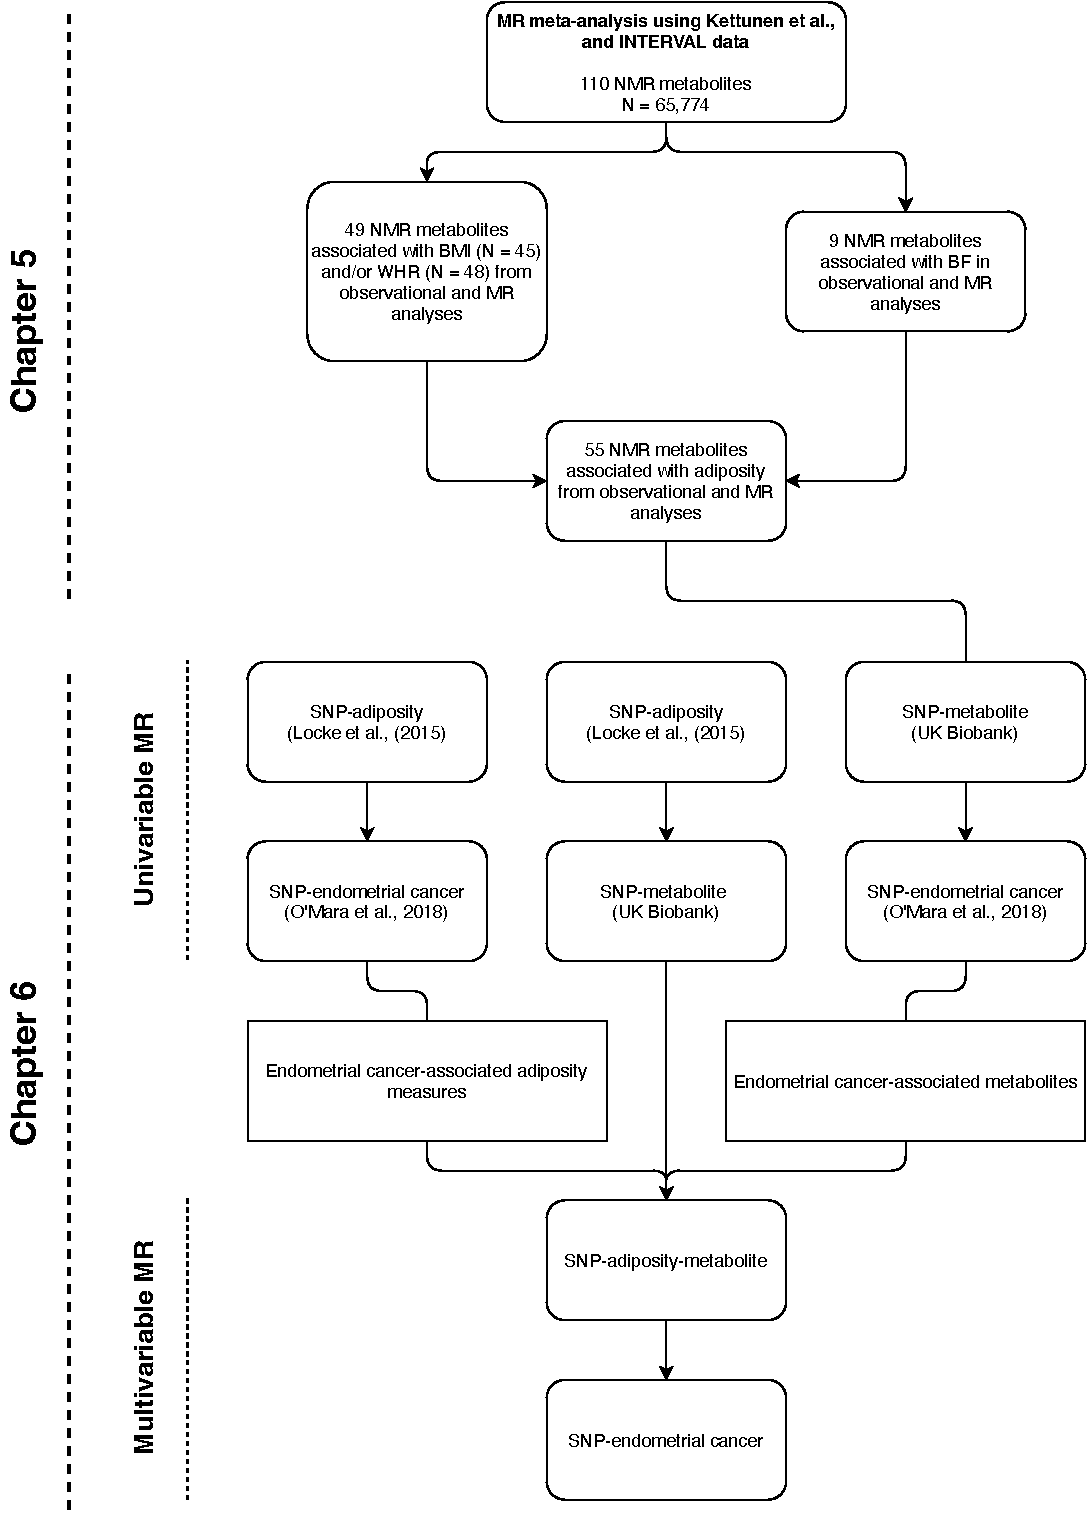
\includegraphics[width=0.98\linewidth]{../index/data/mediation/figures/overview} \caption[Analysis overview]{\textbf{Analysis overview}. In Chapter \ref{MR}, 54 metabolites were identified as being associated with adiposity in a meta-analysis using data from Kettunen et a., (2016)\textsuperscript{\protect\hyperlink{ref-Kettunen2016}{335}} and INTERVAL (unpublished and provided by Adam Butterworth, University of Cambridge). For body mass index (BMI) and waist hip ratio (WHR) these metabolites were identified through directional consistency and multiple testing thresholds across Mendelian randomization (MR) and observational analyses. For body fat percentage (BF) metabolites were identified through directional consistency and a multiple testing threshold in the observational analysis only. These 54 metabolites were taken forward and used in two-sample univariable MR and multivariable MR analyses to investigate intermediate effects on endometrial cancer. NMR = nuclear magnetic resonance.}\label{fig:mediation-figure-analysis-flow}
\end{figure}
\hypertarget{mediation-methods-instrumentation}{%
\subsection{Instrumentation}\label{mediation-methods-instrumentation}}

As discussed in Chapter \ref{MR} Section \ref{MR-methods-instrumentation}, instrumentation of exposures is primarily achieved using either single genetic variants or multiple genetic variants as instrumental variables. Using multiple genetic variants in an instrument which, collectively, explain a greater proportion of the trait variance than any one individual variant can mitigate weak instrument bias. Generally, instruments are obtained from the largest and most recent GWAS using a genome-wide significance threshold of p-value \textless{} 5 x 10\textsuperscript{-8}. This was the most common approach used for instrumenting adiposity measures identified in the systematic review (Chapter \ref{systematic-review}) and was implemented in Chapter \ref{MR}. Few of these studies reported on the independence of SNPs (e.g., a linkage disequilibrium (LD) r\textsuperscript{2} and distance threshold). Similar approaches have been used for studies investigating the association between metabolites and outcomes using an MR framework\textsuperscript{\protect\hyperlink{ref-Bull2020}{415},\protect\hyperlink{ref-Lord2021}{419},\protect\hyperlink{ref-Qian2021}{421},\protect\hyperlink{ref-Qin2020}{422},\protect\hyperlink{ref-Lotta2016}{592}--\protect\hyperlink{ref-Thomas2021}{595}}. Many of these metabolite MR studies did report on the independence of SNPs, however approaches were varied (e.g., LD r\textsuperscript{2} thresholds of 0.1, 0.05, and 0.001) and thresholds appeared arbitrarily set.

\par

Potential overlap in was considered when selecting instruments for adiposity measures and metabolites. In two-sample univariable MR analyses, overlap between datasets providing summary statistics for the exposure and outcome may bias estimates in the presence of weak instruments. This bias may be exacerbated with greater overlap in the two samples. However, given a strong enough instrument, bias as a result of overlap will be close to the un-biased estimate\textsuperscript{\protect\hyperlink{ref-Burgess2016}{441}}. For continuous outcomes (e.g., the association between adiposity measures and metabolites), bias away from the null is a linear function of the sample overlap (e.g., sample overlap of 50\% leads to a bias of 5\%). For binary outcomes (e.g., the association between adiposity measures and metabolites with endometrial cancer), when the association between the SNP and outcome is estimated in all participants, bias is similar to that for a continuous outcome. Where the association between the SNP and outcome is estimated in controls only, unbiased estimates can be obtained\textsuperscript{\protect\hyperlink{ref-Burgess2016}{441}}.

\par

UK Biobank is large and deeply phenotyped prospective sudy which recruited 502,639 participants aged 37--70 years in 22 assessment centres across the United Kingdom\textsuperscript{\protect\hyperlink{ref-Sudlow2015}{596}}. In 2021, NMR data\textsuperscript{\protect\hyperlink{ref-Bell2021a}{544},\protect\hyperlink{ref-Julkunen2021}{597}} and corresponding GWAS data became available for 118,466 UK Biobank individuals, and represents the largest single study of its kind. Sex-specific GWAS data were also made available. Given the large sample size, ability to use sex-specific estimates of the association between genetic variation and metabolites and, desire to obtain the best possible SNP-metabolite estimates for MR analyses, UK Biobank metabolomic data were used here. However, as almost all individuals from UK Biobank were included in the GWAS for BMI (Yengo et al., (2018)\textsuperscript{\protect\hyperlink{ref-Yengo2018}{53}}) and WHR (Pulit et al., (2019)\textsuperscript{\protect\hyperlink{ref-Pulit2019}{54}}) used in the main analysis of Chapter \ref{MR}, overlap with the UK Biobank data were highly likely. As such, summary statistics for BMI and WHR were obtained from GWAS which did not include UK Biobank. Data from these GWAS (discussed in detail in th next section) were used in additional analyses in Chapter \ref{MR} and showed highly consistent associations with metabolites when compared to the BMI and WHR instruments obtained from Yengo et al., (2018) and Pulit et al., (2019), respectively. As such, there is no overlap between adiposity data and metabolite data used in analyses here. However, as the largest available endometrial cancer GWAS, with information on subtypes, included individuals from UK Biobank, there is potential overlap between metabolite data and overall endometrial cancer data. In analyses here, the potential overlap between metabolite GWAS data and endometrial cancer GWAS data is a maximum of 5\%, which is expected to equate to \textasciitilde0.5\% increased false positive rate. These data sources are described in full in the next section.

\par

In this chapter, genetic variants were identified from summary statistics of GWAS for adiposity measures using a genome-wide significance threshold of p-value \textless{} 5 x 10\textsuperscript{-8} and no LD r\textsuperscript{2} and distance threshold. An LD r\textsuperscript{2} and distance threshold was not set as results from additional analyses in Chapter \ref{MR} of the association between adiposity measures and metabolites using clumped and non-clumped instruments, did not identify a difference in effect estimates as a result of clumping. For metabolites, as no investigation of different instrumentation approaches has been conducted and, given studies appear to arbitrarily set LD r\textsuperscript{2} and distance thresholds and there is likely a common genetic architecture across metabolites, genetic variants were identified using a genome-wide significance threshold of p-value \textless{} 5 x 10\textsuperscript{-8} and a conservative LD r\textsuperscript{2} (0.001) and distance threshold (10,000 bases).

\par

\hypertarget{data-1}{%
\subsection{Data}\label{data-1}}

The following section details a number of GWAS and meta-analyses of previously published studies, which were used in this Chapter to perform MR analyses and are required as per STROBE-MR guidelines\textsuperscript{\protect\hyperlink{ref-DaveySmith2019}{440}}. I was not not directly involved in these GWAS. The total sample size (N) and sex-specific sample size does not always tally, this is due to variation in the sample size for each SNP. Where this is the case, `sample size up-to' is used. Due to the way in which studies report GWAS differently, information present in one study (such as sex-specific sample sizes) are not always present in another.

\par

\hypertarget{exposures-adiposity}{%
\subsubsection{Exposures: Adiposity}\label{exposures-adiposity}}

\hypertarget{body-mass-index-1}{%
\paragraph{Body mass index}\label{body-mass-index-1}}

Detailed information is presented in Chapter \ref{MR} Section \ref{MR-exposures-adiposity}. Briefly, summary statistics for the association between genetic variation and BMI were obtained from Locke et al.~(2015)\textsuperscript{\protect\hyperlink{ref-Locke2015}{48}}, in which 322,154 individuals of European ancestries were included in a fixed effects inverse variance weighted meta-analysis. A total of 82 GWAS and 43 studies using the Metabochip array were included in the meta-analysis. Individual GWAS were adjusted for age, age squared, and study specific covariates with residuals inverse rank normally transformed. Imputation was performed using HapMap phase II Utah residents of Northern and Western European ancestries (CEU) reference panel. Each study used a linear regression model assuming an additive genetic model with quality control following procedures outlined previously\textsuperscript{\protect\hyperlink{ref-Winkler2014}{598}}. A fixed effects inverse variance weighted meta-analysis was performed using METAL for the 82 GWAS and 43 studies using the Metabochip array separately. The final meta-analysis combined the single nucleotide polymorphisms (SNPs) found in both the meta-analyses of GWAS and Metabochip studies that underwent genomic control. A total of 77 loci reaching genome-wide significance (p-value \(\leq\) 5x10\textsuperscript{-8}) and separated by at least 500 kilobases were identified. These SNPs explained \textasciitilde2\% of the variance in BMI. All 77 SNPs identified by Locke et al., (2015) were also identified in the Yengo et al., (2018) BMI GWAS used in Chapter \ref{MR}.

\par

\hypertarget{waist-hip-ratio-1}{%
\paragraph{Waist hip ratio}\label{waist-hip-ratio-1}}

Detailed information is presented in Chapter \ref{MR} Section \ref{MR-exposures-adiposity}. Briefly, summary statistics for the association between genetic variation and WHR were obtained from Shungin et al.~(2016)\textsuperscript{\protect\hyperlink{ref-Shungin2015}{49}}, in which 210,088 individuals of European ancestries were included in a fixed effects inverse variance weighted meta-analysis. A total of 57 GWAS and 44 studies using the Metabochip array were included in the meta-analysis. WHR was adjusted for age, age squared, study-specific covariates if necessary with residuals inverse rank normally transformed. Imputation was performed using HapMap phase II CEU reference panel. Each study used a linear regression model assuming an additive genetic model. The final meta-analysis combined the SNPs found in both the meta-analyses of GWAS and Metabochip studies that underwent genomic control. A total of 26 loci reaching genome-wide significance (p-value \(\leq\) 5x10\textsuperscript{-8}) and separated by at least 500 kilobases were identified. The variance explained for these SNPs was not reported, however it will be lower than the 3\% variance explained by the 316 SNPs identified by Pulit et al., (2019)\textsuperscript{\protect\hyperlink{ref-Pulit2019}{54}}. All 26 SNPs identified by Shungin et al., (2016) were also identified in the Pulit et al., (2019) WHR GWAS used in Chapter \ref{MR}.

\par

\hypertarget{body-fat-percentage-1}{%
\paragraph{Body fat percentage}\label{body-fat-percentage-1}}

Detailed information is presented in Chapter \ref{MR} Section \ref{MR-exposures-adiposity}. Briefly, summary statistics for the association between genetic variation and BF were obtained from Lu et al., (2016)\textsuperscript{\protect\hyperlink{ref-Lu2016}{51}}, in which 89,300 individuals of European ancestries were included in a fixed effects inverse variance weighted meta-analysis. A total of 43 GWAS and 13 studies using the Metabochip array were included in the meta-analysis. Individual GWAS were adjusted for age, age squared, and study specific covariates with residuals inverse rank normally transformed. Imputation was performed using HapMap phase II European reference panel. Each study used a linear regression model assuming an additive genetic model. A fixed effects inverse variance weighted meta-analysis was performed using METAL for the 43 GWAS and 13 studies using the Metabochip array separately. The final meta-analysis combined the SNPs found in both the meta-analyses of GWAS and Metabochip studies that underwent genomic control. A total of 7 loci reaching genome-wide significance (p-value \(\leq\) 5x10\textsuperscript{-8}) and separated by at least 1 mega base were identified. Estimation of the variance explained was not available in the European ancestries meta-analysis. In a meta-analysis of individuals of all ancestries, which included up to 11,419 additional individuals of non-European ancestries, these 7 SNPs explained 0.416\% of the variance in BF. The additional 5 SNPs identified in this all ancestries meta-analysis explained 0.58\% of the variance in BF. Two of the identified SNPs (rs6738627 and rs2943650) have previously been associated with favourable adiposity\textsuperscript{\protect\hyperlink{ref-Yaghootkar2014}{47},\protect\hyperlink{ref-Yaghootkar2016}{557}}, which has been associated with increased BF, BMI, fat mass, and reduced fat free mass while simultaneously being associated with reduced risk of type-2 diabetes, hypertension, and heart disease, as well as more favourable blood pressure\textsuperscript{\protect\hyperlink{ref-Yaghootkar2016}{557}}. In additional analyses conducted in Chapter \ref{MR}, comparison of the effect of BF on metabolites, instrumenting BF with the 7 SNPs identified by Lu et al.~and a 5-SNP instrument that did not include the two favourable adiposity SNPs, resulted in tighter confidence intervals (CIs) for the 5-SNP instrument. Additionally, a number of effect estimates reversed in direction when instrumenting BF using the 5 SNPs. As these favourable adiposity SNPs are likely adding noise to the instrumentation of BF, the 5-SNP instrument was used herein. The variance explained by these 5 SNPs will be lower than the variance explained by the 7 SNPs in the all ancestries meta-analysis.

\par

\hypertarget{intermediates-metabolites}{%
\subsubsection{Intermediates: Metabolites}\label{intermediates-metabolites}}

A total of 54 metabolites were identified as being associated with adiposity in Chapter \ref{MR}; two metabolites, associated with BMI and WHR (serum total triglycerides) and BF (estimated description of fatty acid chain length not actual carbon number) were not available in the UK Biobank GWAS. Female-specific summary statistics for each metabolite was obtained from UK Biobank (Borges 2021, unpublished), in which, 118,466 women of European ancestries were included in a linear mixed model GWAS. UK Biobank is a prospective cohort study of \textasciitilde500,000 individuals from the United Kingdom aged 37--70 with a host of genetic and phenotypic data\textsuperscript{\protect\hyperlink{ref-Bycroft2018}{552},\protect\hyperlink{ref-Sudlow2015}{596}}. Un-fasted individuals were selected at random to undergo high-throughput nuclear magnetic resonance (NMR) metabolomic analysis\textsuperscript{\protect\hyperlink{ref-Julkunen2021}{597}} using the Nightingale Health Ltd biomarker quantification\textsuperscript{\protect\hyperlink{ref-Soininen2009}{514},\protect\hyperlink{ref-Wurtz2017}{599}} (version 2020); the same platform for which metabolomic data were avaialble from the Avon Longitudinal Study of Parents and Children (ALSPAC) used in Chapter \ref{observational} and datasets used in Chapter \ref{MR}. All metabolites were inverse rank normally transformed prior to genome-wide analysis. Genome-wide association analysis was performed using the Medical Research Council, Integrative Epidemiology Unit (MRC IEU) UK Biobank GWAS pipeline\textsuperscript{\protect\hyperlink{ref-Mitchell2019}{600}}. A linear mixed model using BOLT-LMM, adjusting for genotype array and fasting time was fit for 118,466 individuals. Population structure was controlled for using 143,006 directly genotyped SNPs (minor allele frequency \textgreater{} 0.01; genotyping rate \textgreater{} 0.015; Hardy-Weinberg equilibrium p-value \textless{} 0.0001 and linkage disequilibrium (LD) pruning to an R\textsuperscript{2} threshold of 0.1 using PLINKv2.00). Borges et al., had not identified lead SNPs at the time of writing. Lead SNPs were thus identified as those reaching a genome-wide significance threshold (p-value \(\leq\) 5x10\textsuperscript{-8}) and which were retained after clumping using a LD r\textsuperscript{2} threshold of 0.001 for SNPs within a 10,000 base window of each other and using the 1000 Genomes version 3 reference panel.

\par

\hypertarget{outcomes-endometrial-cancer}{%
\subsubsection{Outcomes: Endometrial cancer}\label{outcomes-endometrial-cancer}}

Female-specific summary statistics for endometrial cancer were available from O'Mara et al.~(2018)\textsuperscript{\protect\hyperlink{ref-OMara2018}{489}}. This data included summary statistics on overall endometrial cancer as well as endometrioid and non-endometrioid cancer. Briefly, 17 studies on endometrial cancer including 12,906 cases and 108,979 country-matched controls of European ancestries were included in a fixed effects inverse variance weighted meta-analysis. Genotypes were imputed using the 1000 Genomes Project v3 reference panel or a combined 1000 Genomes (V3) UK10K reference panel. In each study, univariate GWAS were conducted adjusting for principal components (PCs). The analysis was repeated for endometrioid only (cases = 8,758; controls = 108,979) and non-endometrioid only (case = 1,230; controls = 108,979) cancers. Overall endometrial cancer included the cases from the endometrioid and non-endometrioid cancers alongside a number of other unclassified cases. Of the 12,906 cases and 108,979 controls for overall endometrial cancer, 636 cases (5\%) and 62,853 controls (58\%) were from UK Biobank. For endometrioid and non-endometrioid cancer, no cases and 62,853 controls (58\%) were from UK Biobank.

\par

\hypertarget{mediation-methods-2smr}{%
\subsection{Two-sample univariable Mendelian randomization}\label{mediation-methods-2smr}}

Summary statistics for the association between genetic variation and BMI\textsuperscript{\protect\hyperlink{ref-Locke2015}{48}}, WHR\textsuperscript{\protect\hyperlink{ref-Shungin2015}{49}}, and BF\textsuperscript{\protect\hyperlink{ref-Lu2016}{51}} were obtained from published GWAS, as described above, all genetic instruments are available on \href{https://github.com/mattlee821/000_thesis/blob/master/index/data/mediation/tables/adiposity_snps.txt}{GitHub}. As summary statistics of the association between genetic variation on metabolites in UK Biobank were unpublished, all genetic instruments are available on \href{https://github.com/mattlee821/000_thesis/blob/master/index/data/mediation/analysis/003_metabolite_endometrial/exposure_data.txt}{GitHub}, alongside a list of metabolites \href{https://github.com/mattlee821/000_thesis/blob/master/index/data/mediation/tables/metabolites.txt}{GitHub} which is also available in the Appendix (Table \ref{tab:appendix-mediation-table-metabolites}).

\par

For all exposures, the following summary-level data were obtained from the original GWAS publications for each exposure-related genetic variant: rsID, effect allele, other/non-effect allele, effect allele frequency, effect estimate, standard error of the effect estimate, p-value, sample size, and units. All exposure-related genetic variants were obtained for each outcome separately. Genetic variants were extracted from each outcome GWAS and, where these were not present, proxy SNPs were included if LD was \(\geq\) 0.8. For proxy SNPs, the inclusion of SNPs where the reference strand was ambiguous (strand flips) was allowed and the reference strand was inferred using a MAF threshold. That is, the reference strand was inferred using a MAF, so long as that MAF was not \(\geq\) 0.3, in which case it was excluded. Exposure and outcome summary statistics for each of the exposure-related SNPs were harmonised in reference to the exposure effect allele being on the increasing scale. For included alleles where the reference strand was ambiguous, the positive strand was inferred using effect allele frequency. That is, if the effect allele frequency of a SNP was not \(\geq\) 0.3 or \(\leq\) 0.7, the reference strand was inferred using the effect allele frequency to harmonise exposure and outcome data; otherwise, it was removed.

\par

Instruments for adiposity measures were not clumped as the studies from which they were obtained stated they were independent or near-independent and analysis in Chapter \ref{MR} indicated clumping did not considerably alter associations with metabolites. Instruments for metabolites were identified using a genome-wide significance threshold of p-value \(\leq\) 5x10\textsuperscript{-8} and an LD r\textsuperscript{2} threshold of 0.001 for SNPs within a 10,000 base window of each other and using the 1000 Genomes reference panel using the \texttt{TwoSampleMR}\textsuperscript{\protect\hyperlink{ref-Hemani2018}{547}} \texttt{R}. To assess the possibility of weak instrument bias, F-statistics were calculated for each exposure-related SNP and an average F-statsistic was calculated for each exposure.

\par

An inverse variance weighted (IVW), multiplicative random effects (IVW-MRE) model was used to estimate the effect of each exposure on the outcome. The model assumes that the strength of the association of the genetic instruments with the exposure is not correlated with the magnitude of the pleiotropic effects and that the pleiotropic effects have an average value of zero\textsuperscript{\protect\hyperlink{ref-Bowden2017}{555}}. Where the number of instruments was not sufficient for an IVW-MRE model, the Wald ratio was used. As analysis presented in this chapter, which aimed to assess the potentially intermediary role of metabolites in the relationship between adiposity and endometrial cancer, aimed to validate results presented in Chapters \ref{systematic-review}, \ref{observational}, and \ref{MR}, no multiple testing threshold was set. Both the adiposity measures and metabolites were inverse rank normally transformed prior to genome-wide analysis and represent standard deviation (SD) units. For MR analyses using these measures, effect estimates are given in SD units. Results testing for the causal effect of both adiposity and metabolites on endometrial cancer are given as odds ratios (OR) and represent the odds of developing endometrial cancer per SD unit increase in the exposure.

\par

\hypertarget{sensitivity-analysis}{%
\subsubsection{Sensitivity analysis}\label{sensitivity-analysis}}

Where possible (i.e., where there were three or more instruments), the assumptions of no pleiotropy among genetic instruments and outcomes were explored using: MR-Egger\textsuperscript{\protect\hyperlink{ref-Bowden2015}{368}}, weighted median\textsuperscript{\protect\hyperlink{ref-Burgess2017a}{369}}, and weighted mode\textsuperscript{\protect\hyperlink{ref-Hartwig2017}{370}} based estimators. These methods are sensitive to the effects of potential pleiotropy. No p-value threshold requirements were set for these methods, instead consistency between the IVW-MRE model and these methods was investigated. Briefly, MR-Egger provides an estimate of unbalanced or directional horizontal pleiotropy via the intercept of a linear regression of the SNP-exposure and SNP-outcome association. In the presence of pleiotropy, the intercept will be biased away from the origin. MR-Egger gives consistent estimates when 100\% of genetic instruments are invalid\textsuperscript{\protect\hyperlink{ref-Bowden2015}{368}}. The weighted median is complimentary to MR-Egger but does not rely on the ``instrument strength independent of direct effect'' (InSIDE) assumption. It calculates the median of an empirical distribution of the causal effect estimates weighted for precision. It provides consistent estimates when at least 50\% of the weight comes from valid genetic instruments and as long as no one genetic instrument contributes \textgreater{} 50\% of the weight\textsuperscript{\protect\hyperlink{ref-Burgess2017a}{369}}. The weighted mode assumes the true causal effect is the most common effect and it is robust when the majority of effect estimates are derived from valid instruments\textsuperscript{\protect\hyperlink{ref-Hartwig2017}{370}}.

\par

\hypertarget{two-sample-multivariable-mendelian-randomization}{%
\subsection{Two-sample multivariable Mendelian randomization}\label{two-sample-multivariable-mendelian-randomization}}

All adiposity measures were included in the MVMR analysis. Of the metabolites included in the two-sample univariable MR analysis estimating the causal effect of adiposity on metabolites and of metabolites on endometrial cancer, only those which showed a consistent direction of effect with both adiposity and endometrial cancer were included in the MVMR analyses. That is, if an adiposity measure increased a metabolite, that metabolite increased endometrial cancer, and taht adiposity measure increased endometrial cancer, then the metabolite was considered as a potential intermediate. Or, if an adiposity measure decreased a metabolite, that metabolite decreased endometrial cancer, and that adiposity measure increased endometrial cancer, then the metabolite was considered a potential intermediate. Otherwise, the metabolite was excluded from MVMR analyses.

\par

In MVMR, SNPs associated with the exposure (adiposity) and proposed intermediate (metabolites) were combined to create a combined instrument of the exposure and intermediate. This combined SNP list was used to extract instruments from both GWASs of the exposure and the intermediate metabolite. The resulting instrument was then clumped to remove duplicate SNPs and, SNPs in LD with one another to avoid overestimation of effects using the same clumping thresholds as with the univariable analysis described above (LD r\textsuperscript{2} \textgreater{} 0.001 and 10,000 base window).

\par

The resulting instrument contains SNPs associated with both the exposure and intermediate; extracting data from the GWAS of the exposure gives an instrument for the exposure adjusted for the intermediate, and extracting data from the GWAS of the intermediate gives an instrument for the intermediate adjusted for the exposure (Figure \ref{fig:mediation-figure-mvmr-dag}). As such, instruments for BMI and instruments for metabolites will use the same SNPs but different estimates. For example, a BMI instrument adjusted for metabolite 1 will include the SNPs associated with BMI and the SNPs associated with metabolite 1, with all data extracted from the GWAS of BMI. An instrument for metabolite 1 adjusted for BMI will include the SNPs associated with BMI and the SNPs associated with metabolite 1, with all data extracted from the GWAS of metabolite 1. The following process was followed for obtaining instruments:

\par
\begin{enumerate}
\def\labelenumi{\arabic{enumi}.}
\tightlist
\item
  SNPs associated with each adiposity measure and each metabolite were identified in the same way as for the two-sample univariable MR analysis described previously (\ref{mediation-methods-2smr}).
\item
  Identified SNPs for each adiposity and metabolite pair were combined to create a SNP list for each adiposity and metabolite pair.
\item
  These SNP lists were used to extract summary level data for instruments (rsID, effect allele, other/non-effect allele, effect allele frequency, effect estimate, standard error of the effect estimate, p-value, N, and units) from the GWASs of each adiposity measure and each metabolite individually.
\item
  Each instrument was clumped using the \texttt{TwoSampleMR}\textsuperscript{\protect\hyperlink{ref-Hemani2018}{547}} \texttt{R} package setting an LD R\textsuperscript{2} threshold of 0.001 for SNPs within a 10,000 base window of each other and using the 1000 Genomes reference panel.
\item
  Data for each adiposity and metabolite pair were harmonised in reference to the adiposity-increasing effect allele in the adiposity instrument .
\item
  Instruments for each adiposity and metabolite pair were extracted from the endometrial cancer GWAS using MR-Base. Where SNPs were not present in the outcome GWAS, proxy SNPs were included if LD was \(\geq\) 0.8. For proxy SNPs, the inclusion of SNPs where the reference strand was ambiguous (strand flips) was allowed and the reference strand was inferred using a MAF threshold of 0.3.
\item
  Exposure-related SNPs from summary level data of the outcome were harmonised in reference to the adiposity-increasing effect allele in the adiposity instrument instrument.
\end{enumerate}



\begin{figure}

{\centering \includegraphics[width=0.75\linewidth]{thesis_files/figure-latex/mediation-figure-mvmr-dag-1} 

}

\caption[Directed acyclic graph of multivariable MR principle]{\textbf{Directed acyclic graph of the multivariable Mendelian randomization principle using two exposures}. The directed acyclic graph illustrates the principle of multivariable Mendelian randomization (MR) using an exposure (X1) and a mediator (X2) on a single outcome. Genetic instruments (G) associated with X1 and X2 are combined into an instrument. In this example, the instrument includes G1, G2, and any number of other SNPs (Gn). The instrument is extracted from summary statistics for each of X1 and X2. G = single nucleotide polymorphism; X1 = exposure, X2 = mediator; Y = outcome; U = unmeasured confounding}\label{fig:mediation-figure-mvmr-dag}
\end{figure}
For MVMR analysis, the SNP, effect estimate, and standard error for each exposure (adiposity and metabolite) and outcome are required. Instrument strength for each exposure was estimated using a generalized version of Cochran's Q\textsuperscript{\protect\hyperlink{ref-Sanderson2019b}{601},\protect\hyperlink{ref-Sanderson2021a}{602}}, using the \texttt{strength\_mvmr()} function in the \texttt{MVMR} \texttt{R} package assuming a pairwise covariance of 0. The assumption being that the SNP-exposure association and the SNP-intermediate association are estimated in independent samples (e.g., two different GWAS of independent populations). Horizontal pleiotropy was evaluated using a modified form of Cochran's Q using the \texttt{pleiotropy\_mvmr()} function in the \texttt{MVMR} \texttt{R} package and assuming a pairwise covariance of 0.

\par

An IVW MVMR model was used to obtain the direct causal effect of each adiposity measure adjusted for each metabolite and each metabolite adjusted for each adiposity measure on endometrial cancer risk. The aim of this analysis was to inform whether the effect of adiposity on endometrial cancer is partly explained by the effect of adiposity on metabolites and the effect of those metabolites on endometrial cancer or whether any effects of adiposity and metabolites on endometrial cancer are independent. Results are presented as OR and represent the odds of developing endometrial cancer per SD unit increase in the exposure.

\par

\hypertarget{results}{%
\section{Results}\label{results}}

For this section, results are presented first for the two-sample univariable MR analyses of the effect of adiposity on endometrial cancer, the effect of adiposity on metabolites in UK Biobank, and the effect of those metabolites for which there was evidence for a causal effect of adiposity (consistent across analyses conducted in Chapter \ref{MR} and UK Biobank here) and endometrial cancer. Finally, results from the two-sample MVMR analyses unpicking the potential intermediary role of these metabolites in the relationship between adiposity and endometrial cancer are presented.

\par

\hypertarget{mediation-results-adiposity-cancer}{%
\subsection{Two-sample univariable Mendelian randomization: association between adiposity measures and endometrial cancer}\label{mediation-results-adiposity-cancer}}

Here, using the largest endometrial cancer GWAS to date, the MR analyses performed as part of this thesis provided strong evidence of a causal effect of BMI on endometrial cancer (OR per SD unit increase in BMI = 1.91; 95\% CI = 1.62--2.25; p-value = 1.74 x 10\textsuperscript{-15}; (Table \ref{tab:mediation-table-adiposity-cancer}). A similar effect (OR = 2.02; 95\% CI = 1.68--2.43; p-value = 1.59 x 10\textsuperscript{-13}) was found for endometrioid cancer, while a smaller effect was observed for non-endometrioid cancer (OR = 1.63; 95\% CI = 1.11--2.39; p-value = 0.01).

\par

The effect of WHR on overall endometrial cancer and endometrioid cancer were directionally consistent but lesser in magnitude than results for BMI (OR = 1.2; 95\% CI = 0.98 - 1.53 and 1.25; 95\% CI = 0.93 - 1.58, respectively). The effect of BF on endometrial cancer (OR = 2.54; 95\% CI = 2.04--3.16; p-value = 1.02 x 10\textsuperscript{-16}), endometrioid (OR = 2.73; 95\% CI = 1.83--4.09; p-value = 9.93 x 10\textsuperscript{-7}), and non-endometrioid (OR = 2.01; 95\% CI = 0.52--7.7; p-value = 0.31) were consistently greater than those observed for BMI, though with wider CIs.

\par

Sensitivity analyses, which included weighted median, weighted mode, and MR-Egger models, were consistent with the IVW-MRE model for each exposure (Appendix Figure \ref{fig:appendix-mediation-figure-forestplot-adiposity-endometrial}). All figures associated with sensitivity analyses (e.g.~leave-one-out analyses) are available on \href{https://github.com/mattlee821/000_thesis/tree/master/index/data/mediation/figures/001_adiposity_endometrial}{GitHub} with representative figures presented in the appendix (Appendix \ref{appendix-mediation}). All results are available on \href{https://github.com/mattlee821/000_thesis/tree/master/index/data/mediation/results/001_adiposity_endometrial}{GitHub}.

\par
\begin{ThreePartTable}
\begin{TableNotes}[para]
\item Results for inverse variance weighted multiplicative random effects model are presented. Odds ratios (OR) and associated 95\% confidence intervals (CI) per standard deviation unit increase in body mass index (BMI), waist hip ratio (WHR), or body fat percentage (BF)
\end{TableNotes}
\begin{longtable}[t]{llrrrl}
\caption{\label{tab:mediation-table-adiposity-cancer}Two-sample univariable Mendelian randomization results of the association between adiposity measures and endometrial cancer}\\
\toprule
 &  & OR & Lower CI & Upper CI & p-value\\
\midrule
\endfirsthead
\caption[]{\label{tab:mediation-table-adiposity-cancer}Two-sample univariable Mendelian randomization results of the association between adiposity measures and endometrial cancer \textit{(continued)}}\\
\toprule
 &  & OR & Lower CI & Upper CI & p-value\\
\midrule
\endhead

\endfoot
\bottomrule
\insertTableNotes
\endlastfoot
\cellcolor{gray!6}{BMI} & \cellcolor{gray!6}{Endometrial cancer} & \cellcolor{gray!6}{1.91} & \cellcolor{gray!6}{1.62} & \cellcolor{gray!6}{2.25} & \cellcolor{gray!6}{7.47e-15}\\
BMI & Endometrioid & 2.02 & 1.68 & 2.43 & 1.6e-13\\
\cellcolor{gray!6}{BMI} & \cellcolor{gray!6}{Non-endometrioid} & \cellcolor{gray!6}{1.63} & \cellcolor{gray!6}{1.11} & \cellcolor{gray!6}{2.39} & \cellcolor{gray!6}{0.0122}\\
BF & Endometrial cancer & 2.54 & 2.04 & 3.16 & 1.02e-16\\
\cellcolor{gray!6}{BF} & \cellcolor{gray!6}{Endometrioid} & \cellcolor{gray!6}{2.73} & \cellcolor{gray!6}{1.83} & \cellcolor{gray!6}{4.09} & \cellcolor{gray!6}{9.94e-07}\\
\addlinespace
BF & Non-endometrioid & 2.01 & 0.52 & 7.70 & 0.31\\
\cellcolor{gray!6}{WHR} & \cellcolor{gray!6}{Endometrial cancer} & \cellcolor{gray!6}{1.26} & \cellcolor{gray!6}{0.95} & \cellcolor{gray!6}{1.66} & \cellcolor{gray!6}{0.103}\\
WHR & Endometrioid & 1.25 & 0.91 & 1.74 & 0.174\\
\cellcolor{gray!6}{WHR} & \cellcolor{gray!6}{Non-endometrioid} & \cellcolor{gray!6}{2.31} & \cellcolor{gray!6}{1.23} & \cellcolor{gray!6}{4.35} & \cellcolor{gray!6}{0.00952}\\*
\end{longtable}
\end{ThreePartTable}
\hypertarget{mediation-results-adiposity-metabolites}{%
\subsection{Two-sample univariable Mendelian randomization: association between adiposity measures and metabolites}\label{mediation-results-adiposity-metabolites}}

A total of 54 metabolites were identified as being associated with BMI (N = 45), WHR (N = 48), and BF (N = 9) in Chapter \ref{MR}. Two of these metabolites, associated with BMI and WHR (serum total triglycerides) and BF (estimated description of fatty acid chain length not actual carbon number) were not available in the UK Biobank GWAS. As such, a total of 44, 47, and 8 metabolites, which were associated with BMI, WHR, and BF in Chapter \ref{MR}, respectively, were available for analysis in UK Biobank.

\par

For BMI, of the 44 metabolites, four had directions of effect that were not consistent with the previous MR analysis (Chapter \ref{MR}), meta-analysis (Chapter \ref{MR}), and observational (Chapter \ref{observational}) analyses: apolipoprotein B, free cholesterol in medium very large low density lipoprotein (VLDL), total lipids in medium VLDL, total lipids in very small VLDL. For WHR, of the 47 metabolites, two had directions of effect that were not consistent with the previous MR analysis (Chapter \ref{MR}), meta-analysis (Chapter \ref{MR}), and observational (Chapter \ref{observational}) analyses: phenylalanine and tyrosine. For BF, all 8 of the analysed metabolites had consistent directions of effect with the previous MR analysis (Chapter \ref{MR}), meta-analysis (Chapter \ref{MR}), and observational (Chapter \ref{observational}) analyses. Sensitivity analyses did not highlight metabolite analyses which violated the MR assumptions. As such, a total of 40, 45, and 8 metabolites (53 unique metabolites) were taken forward for MR analysis to estimate the effect of these metabolites on endometrial cancer outcomes. Seven of these metabolites were only found to be associated with WHR and 5 of these metabolites were uniquely associated with BF. Two metabolites were associated with both BMI and BF and 38 metabolites were associated with both BMI and WHR. Only 1 metabolite, valine, was associated with all three measures.

\par

All results for the investigation of the effect of adiposity measures on metabolites measured in UK Biobank are presented in Figure \ref{fig:mediation-figure-forestplot-adiposity-metabolites} and are available on \href{https://github.com/mattlee821/000_thesis/tree/master/index/data/mediation/results/002_adiposity_metabolite}{GitHub}. All sensitivity plots are available on \href{https://github.com/mattlee821/000_thesis/tree/master/index/data/mediation/figures/002_adiposity_metabolite}{GitHub} and representative figures are presented in the appendix (Appendix \ref{appendix-mediation}).

\par

\newpage
\thispagestyle{empty}
\vspace*{-3cm}




\begin{figure}

{\centering \includegraphics[width=1\linewidth]{data/mediation/figures/002_adiposity_metabolite/forestplot} 

}

\caption[Two-sample univariable Mendelian randomization analysis: association between adiposity measures and metabolites using UK Biobank data]{\textbf{Two-sample univariable Mendelian randomization analysis: association between adiposity measures and metabolites using UK Biobank data}. Effect estimates and associated 95\% confidence intervals shown for an standard deviation (SD) change in metabolite per SD unit higher body mass index (BMI), waist hip ratio (WHR), or body fat percentage (BF). Solid points indicate a nominal p-value threshold of 0.05 has been reached. Available on \href{https://github.com/mattlee821/000_thesis/blob/master/index/data/mediation/figures/002_adiposity_metabolite/forestplot.pdf}{GitHub}.}\label{fig:mediation-figure-forestplot-adiposity-metabolites}
\end{figure}
\hypertarget{mediation-results-metabolites-cancer}{%
\subsection{Two-sample univariable Mendelian randomization: association between adiposity-associated metabolites and endometrial cancer}\label{mediation-results-metabolites-cancer}}

Two-sample univariable MR analysis was used to investigate the causal effect of 53 metabolites (i.e., 40, 45, and 8 metabolites driven by BMI, WHR, and BF, respectively) on endometrial cancer. Instruments for metabolites were obtained from an unpublished GWAS of 249 circulating metabolites performed in UK Biobank (Borges 2021, unpublished). Using a genome-wide p-value threshold of 5x10\textsuperscript{-8} and an LD r\textsuperscript{2} clumping threshold (0.001) for SNPs within a 10,000 base window, to ensure independance of SNPs, 2595 total associations with 53 metabolites were identified (unique number of SNPs = 934; minimum number of SNPs associated with a metabolite = 6, maximum number of SNPs associated with a metabolite = 84; Figure \ref{fig:mediation-figure-metabolites-snp-distribution}). The greater the number of SNPs associated with a trait, the larger the variance explained by those SNPs and thus the power afforded by that instrument in an MR analysis. Of the 934 unique SNPs identified, 54\% of SNPs were associated with just 1 metabolite (Figure \ref{fig:mediation-figure-metabolites-snp-numbers}). The remaining 46\% of SNPs were associated with two or more metabolites, with 1 SNP (rs12154627) associated with 33 metabolites. Metabolites were inverse rank normally transformed prior to genome-wide analysis and represent SD units.

\par

\newpage
\thispagestyle{empty}
\vspace*{-1cm}




\begin{figure}

{\centering \includegraphics[width=0.8\linewidth]{thesis_files/figure-latex/mediation-figure-metabolites-snp-distribution-1} 

}

\caption[Distribution of the number of SNPs with which metabolites were associated.]{\textbf{Distribution of the number of SNPs with which metabolites were associated}. A total of 934 unique single nucleotide polymorphisms (SNPs) were identified across 53 metabolites. The number of SNPs associated with each metabolite varied between 6 and 84 with a mean of 49. Bin size = 10.}\label{fig:mediation-figure-metabolites-snp-distribution}
\end{figure}



\begin{figure}

{\centering \includegraphics[width=0.8\linewidth]{thesis_files/figure-latex/mediation-figure-metabolites-snp-numbers-1} 

}

\caption[Distribution of the number of metabolites with which individual SNPs were associated]{\textbf{Distribution of the number of metabolites with which individual SNPs were associated}. The majority of the 934 identified single nucleotide polymorphisms (SNPs) were associated with one metabolite. One SNP was associated with 33 out of a total 53 metabolites. Bin size = 1.}\label{fig:mediation-figure-metabolites-snp-numbers}
\end{figure}
\newpage

A total of 5 metabolites showed evidence of association for at least one outcome (Figure \ref{fig:mediation-figure-forestplot-metabolites-cancer}). Valine was the only metabolite found to be negatively associated with the risk of endometrial cancer (OR of endometrial cancer per SD unit increase in valine = 0.82; 95\% CI = 0.69--0.98; p-value = 0.03), which was directionally consistent with both endometrioid and non-endometrioid cancers. The largest effect was found for triglycerides in small VLDL, which increased the odds of non-endometrioid cancer by 1.79 (95\% CI = 1.25--2.56; p-value = 0.001), which was directionally consistent with results for overall endometrial cancer and endometrioid cancer. The largest effect on endometrioid cancer was for phospholipids in very large high density lipoprotein (HDL; OR = 1.16; 95\% CI = 1.01--1.35; p-value = 0.04), results of which were consistent for overall endometrial cancer but opposite to those found in non-endometrioid cancer (though, CIs overlapped all analysis results and the null). The largest effect on overall endometrial cancer was for triglycerides in very large HDL (OR = 1.11; 95\% CI = 1--1.24;2; p-value = 0.06), which was directionally consistent with both endometrioid and non-endometrioid cancers. For triglycerides in very small VLDL, effects were largest for non-endometrioid cancer (OR = 1.56; 95\% CI = 1.12--2.17;; p-value = 0.008), which was directionally consistent with results for overall endometrial cancer and endometrioid cancer.

\par

Of the 5 metabolites with evidence of an association with endometrial cancer, endometrioid cancer, and/or non-endometrioid cancer, only triglycerides in very large HDL was associated with BF in the previous analysis conducted in this chapter and in observational (Chapter \ref{observational}) and MR (Chapter \ref{MR}) analyses. The remaining four metabolites were not associated with BF in any analysis, but were all associated with BMI and WHR in the previous analysis here and in observational (Chapter \ref{observational}) and MR (Chapter \ref{MR}) analyses. As all 5 metabolites showed evidence of association with a measure of adiposity and endometrial cancer, all were considered for MVMR analysis. All results are available on \href{https://github.com/mattlee821/000_thesis/tree/master/index/data/mediation/results/003_metabolite_endometrial}{GitHub} and presented in Appendix Figure \ref{fig:appendix-mediation-figure-forestplot-metabolites-cancer} which is also available on \href{https://github.com/mattlee821/000_thesis/blob/master/index/data/mediation/figures/003_metabolite_endometrial/forestplot_all.pdf}{GitHub}. Figures for sensitivity analyses are also on \href{https://github.com/mattlee821/000_thesis/tree/master/index/data/mediation/figures/003_metabolite_endometrial}{GitHub}.

\par




\begin{figure}
\includegraphics[width=1\linewidth]{../../007_metabolites_outcomes/analysis/003_metabolite_endometrial/figures/forestplot} \caption[Two-sample univariable Mendelian randomization analysis: association between metabolites and endometrial cancer using UK Biobank data]{\textbf{Two-sample univariable Mendelian randomization analysis: association between metabolites and endometrial cancer using UK Biobank data}. Forest plot shows odds ratio (OR) and 95\% confidence interval for metabolites associated with body mass index, waist hip ratio, and/or body fat percentage with endometrial cancer, endometrioid cancer, and non-endometrioid cancer. Data are presented for endometrial-associated metabolites. The main analysis (inverse variance weighted multiplicative random effects (IVW-MRE)) is presented alongside sensitivity analyses (weighted median, weighted mode, MR-Egger). Available on \href{https://github.com/mattlee821/000_thesis/blob/master/index/data/mediation/figures/003_metabolite_endometrial/forestplot.pdf}{GitHub}.}\label{fig:mediation-figure-forestplot-metabolites-cancer}
\end{figure}
\hypertarget{two-sample-multivariable-mendelian-randomization-intermediate-effects-of-adiposity-associated-metabolites-in-the-association-between-adiposity-measures-and-endometrial-cancer}{%
\subsection{Two-sample multivariable Mendelian randomization: intermediate effects of adiposity-associated metabolites in the association between adiposity measures and endometrial cancer}\label{two-sample-multivariable-mendelian-randomization-intermediate-effects-of-adiposity-associated-metabolites-in-the-association-between-adiposity-measures-and-endometrial-cancer}}

Of the 5 metabolites for which there was causal evidence of an effect of at least one measure of adiposity and an effect on endometrial cancer, two had directions of effect that were consistent with a potential intermediate role: triglycerides in small VLDL and triglycerides in very small VLDL. Of the remaining three metabolites, all three adiposity measures were found to decrease phospholipids in very large HDL and triglycerides in very large HDL, while an increase in these metabolites was associated with an increase in all three endometrial cancer outcomes. The remaining metabolite, valine, was found to be increased by all three adiposity measures, however increased valine was associated with a decreased risk of all three endometrial cancer outcomes. As such, triglycerides in small VLDL and triglycerides in very small VLDL were taken forward for MVMR analysis. Using individual level data from ALSPAC adults used in Chapter \ref{observational} (N = 3,305; data not shown), the Spearman's Rho correlation between the two metabolites was 0.9.

\par

Results from the two-sample univariable MR analysis of the association between adiposity measures and triglycerides in small and very small VLDL (Section \ref{mediation-results-adiposity-metabolites}) are presented in Table \ref{tab:mediation-table-mvmr-adiposity-metabolites}. In these analyses, the strongest effect between adiposity measures and triglycerides in small VLDL was found for WHR (SD unit increase in metabolite per SD increase in adiposity measure = 0.56; 95\% CI = 0.26--0.86; p-value = \ensuremath{2.5\times 10^{-4}}). The strongest effect between adiposity measures and triglycerides in very small VLDL was also found for WHR (beta = 0.45; 95\% CI = 0.2--0.7; p-value = \ensuremath{4.5\times 10^{-4}}). The effects of BMI (effect on small VLDL = 0.07; effect on very small VLDL = 0.06) and BF (effect on small VLDL = 0.11; effect on very small VLDL = 0.05) on both metabolites were smaller with CIs that overlapped the null.

\par

\newpage
\begin{ThreePartTable}
\begin{TableNotes}[para]
\item Results are given for the inverse variance weighted multiplicative random effects model. Effect estimates are given as SD unit increase in metabolite per SD unit increase in adiposity measure. Metabolite labels are presented with their originally measured units. BMI = body mass index; WHR = waist hip ratio; BF = body fat percentage; VLDL = very large low density lipoprotein.
\end{TableNotes}
\begin{longtable}[t]{llllll}
\caption{\label{tab:mediation-table-mvmr-adiposity-metabolites}Two-sample univariable Mendelian randomization: association between adiposity measures and triglycerides in small and very small VLDL}\\
\toprule
Exposure & Metabolite (units) & Effect & Lower CI & Upper CI & p-value\\
\midrule
\cellcolor{gray!6}{BMI} & \cellcolor{gray!6}{Triglycerides in small VLDL (mmol/l)} & \cellcolor{gray!6}{0.07} & \cellcolor{gray!6}{-0.002} & \cellcolor{gray!6}{0.14} & \cellcolor{gray!6}{0.06}\\
WHR & Triglycerides in small VLDL (mmol/l) & 0.56 & 0.26 & 0.86 & 0.0002\\
\cellcolor{gray!6}{BF} & \cellcolor{gray!6}{Triglycerides in small VLDL (mmol/l)} & \cellcolor{gray!6}{0.11} & \cellcolor{gray!6}{-0.01} & \cellcolor{gray!6}{0.23} & \cellcolor{gray!6}{0.08}\\
BMI & Triglycerides in very small VLDL (mmol/l) & 0.06 & -0.002 & 0.13 & 0.06\\
\cellcolor{gray!6}{WHR} & \cellcolor{gray!6}{Triglycerides in very small VLDL (mmol/l)} & \cellcolor{gray!6}{0.45} & \cellcolor{gray!6}{0.19} & \cellcolor{gray!6}{0.7} & \cellcolor{gray!6}{0.0004}\\
\addlinespace
BF & Triglycerides in very small VLDL (mmol/l) & 0.05 & -0.12 & 0.23 & 0.55\\
\bottomrule
\insertTableNotes
\end{longtable}
\end{ThreePartTable}
Results from the two-sample univariable MR analysis of the association between triglycerides in small and very small VLDL with endometrial cancer (Section \ref{mediation-results-metabolites-cancer}) are presented in Table \ref{tab:mediation-table-mvmr-metabolites-endometrial}. In these analyses, the strongest effect for both triglycerides in small (OR per SD unit increase in metabolite = 1.8; 95\% CI = 1.3--2.6; p-value = 0.00141) and very small VLDL (OR = 1.6; 95\% CI = 1.1--2.2; p-value = 0.00786) was for non-endometrioid cancer. Both metabolites had positive effects on endometrioid and overall endometrial cancer with highly similar effect sizes. However, effects were smaller than for non-endometrioid cancer and CIs overlapped the null. These results are presented alongside the MVMR results in Figure \ref{fig:mediation-figure-forestplot-adiposity-metabolites-cancer}.

\par

\newpage

\begingroup\fontsize{10}{12}\selectfont
\begin{ThreePartTable}
\begin{TableNotes}[para]
\item Results are given for the inverse variance weighted multiplicative random effects model. Effect estimates are given as the odds (OR) of endometrial cancer per SD unit increase in metabolite. Metabolite labels are presented with their originally measured units
\end{TableNotes}
\begin{longtable}[t]{llllll}
\caption{\label{tab:mediation-table-mvmr-metabolites-endometrial}Two-sample univariable Mendelian randomization: association between triglycerides in small and very small VLDL and endometrial cancer}\\
\toprule
Exposure & Outcome & OR & Lower CI & Upper CI & p-value\\
\midrule
\cellcolor{gray!6}{Triglycerides in small VLDL (mmol/l)} & \cellcolor{gray!6}{Endometrial cancer} & \cellcolor{gray!6}{1.11} & \cellcolor{gray!6}{0.98} & \cellcolor{gray!6}{1.25} & \cellcolor{gray!6}{0.1}\\
Triglycerides in small VLDL (mmol/l) & Endometroid & 1.11 & 0.96 & 1.28 & 0.16\\
\cellcolor{gray!6}{Triglycerides in small VLDL (mmol/l)} & \cellcolor{gray!6}{Non-endometroid} & \cellcolor{gray!6}{1.79} & \cellcolor{gray!6}{1.25} & \cellcolor{gray!6}{2.56} & \cellcolor{gray!6}{0.001}\\
Triglycerides in very small VLDL (mmol/l) & Endometrial cancer & 1.11 & 0.98 & 1.24 & 0.09\\
\cellcolor{gray!6}{Triglycerides in very small VLDL (mmol/l)} & \cellcolor{gray!6}{Endometroid} & \cellcolor{gray!6}{1.11} & \cellcolor{gray!6}{0.96} & \cellcolor{gray!6}{1.27} & \cellcolor{gray!6}{0.15}\\
\addlinespace
Triglycerides in very small VLDL (mmol/l) & Non-endometroid & 1.56 & 1.12 & 2.17 & 0.01\\
\bottomrule
\insertTableNotes
\end{longtable}
\end{ThreePartTable}
\endgroup{}

All results relevant to the MVMR analysis (this includes univariable two-sample MR results) are presented in Figure \ref{fig:mediation-figure-forestplot-adiposity-metabolites-cancer} and Appendix Tables \ref{tab:appendix-mediation-table-mvmr-bmi}, \ref{tab:appendix-mediation-table-mvmr-whr}, and \ref{tab:appendix-mediation-table-mvmr-bf} for BMI, WHR, and BF, respectively. A summary of the MVMR analysis is given herein.

\par

In MVMR analysis, the effect of BMI on overall endometrial cancer was similar after adjustment for either metabolite: OR per SD unit increase in BMI adjusted for triglycerides in small VLDL = 1.9; 95\% CI = 1.57--2.29; p-value = 5.18 x 10\textsuperscript{-9}; OR per SD unit increase in BMI adjusted for triglycerides very small VLDL = 1.87; 95\% CI = 1.53--2.28; p-value = 7.26 x 10\textsuperscript{-8}. These results were similar to the unadjusted (i.e., two-sample univariable MR) effect of BMI on endometrial cancer (OR per SD unit increase in BMI = 1.91; 95\% CI = 1.62--2.25; p-value = 7.47 x 10\textsuperscript{-15}). A similar pattern of association was found across endometrioid and non-endometrioid cancer, with similar effect sizes and CIs after adjustment for each metabolite and when comparing effect size and CIs with the unadjusted effects. The effect for non-endometrioid cancer appeared to attenuate more, but CIs overlapped the two-sample univariable MR results. When looking at the effect of metabolites on all endometrial cancer outcomes after adjustment for BMI, there was little difference with effect size in comparison to the unadjusted effect, however CIs were generally wider in the adjusted estimates. For non-endometrioid cancer, the adjusted effect size was larger than the unadjusted effect size for both metabolites (though, CIs overlapped). Given the similarity between unadjusted and adjusted effects, there was little evidence for an intermediate role of either metabolite on the association between BMI and all endometrial cancer outcomes.

\par

\blandscape
\thispagestyle{empty}




\begin{figure}

{\centering \includegraphics[width=0.95\linewidth]{../../007_metabolites_outcomes/analysis/004_mvmr/figures/forestplot} 

}

\caption[Multivariable Mendelian randomization: intermediate effects of adiposity-associated metabolites in the association between adiposity measures and endometrial cancer]{\textbf{Multivariable Mendelian randomization: intermediate effects of adiposity-associated metabolites in the association between adiposity measures and endometrial cancer}. Forest plot shows odds ratio and 95\% confidence interval for: the two-sample univariable Mendelian randomization (MR) analyses presented in this chapter (Section \ref{mediation-results-adiposity-cancer} and \ref{mediation-results-metabolites-cancer}) and the two-sample multivariable MR results of the intermediary effect of adiposity-associated metabolites and endometrial endometrial (left), endometrioid (middle) and non-endometrioid cancer (right). Points and confidence intervals are coloured for the variable they represent in the two-sample univariable MR and for the adjusted variable in the two-sample multivariable MR, e.g.~body mass index (BMI) is coloured orange and any metabolite effect adjusted for BMI is coloured orange also. An inverse variance weighted model was used. BF = body fat percentage; WHR = waist hip ratio; SVLDLTG = triglycerides in small VLDL; XSVLDLTG = triglycerides in very small VLDL. Available on \href{https://github.com/mattlee821/000_thesis/blob/master/index/data/mediation/figures/004_mvmr/forestplot.pdf}{GitHub}.}\label{fig:mediation-figure-forestplot-adiposity-metabolites-cancer}
\end{figure}
\elandscape

For the effect of BF and WHR on endometrial and endometrioid cancer, a similar pattern of association to that of BMI was seen, with effect sizes and CIs highly similar after adjustment with either metabolite. For example, the effect of WHR on endometrial cancer adjusted for triglycerides in small VLDL was 1.17 (95\% CI = 0.7--1.96; p-value = 0.55) whereas after adjustment for triglycerides in very small VLDL the OR was 1.17 (95\% CI = 0.71--1.93; p-value = 0.55). For both BF and WHR, the adjusted effects had much wider CIs than the unadjusted effects; for BF, adjustment for either metabolite resulted in CIs which crossed the null. For WHR, CIs crossed the null in unadjusted and adjusted analyses. When looking at the metabolites effects on endometrial and endometrioid cancer after adjustment for BF or WHR, there is a similar pattern of association to when adjusting for BMI, with similar sized effect sizes and CIs which overlapped the null. The exception was for the effect of triglycerides in small VLDL on overall endometrial cancer, where, when adjusted for BF (OR = 1.39; 95\% CI = 1.04--1.87; p-value = 0.02) the CIs did not cross the null unlike in the unadjusted analysis (OR = 1.11; 95\% CI = 0.98--1.25; p-value = 0.1), but CIs overlapped between both analyses.

\par

For non-endometrioid cancer, the pattern of association for BF and WHR was different to that of BMI. For BF, adjustment for triglycerides in small VLDL resulted in directions of effect that were opposite to the unadjusted (univariable) MR estimate (BF-adjusted OR = 0.98; 95\% CI = 0.41--2.35; p-value = 0.96; BF-unadjusted OR = 2.01; 95\% CI = 0.52--7.7; p-value = 0.31). The same was true for WHR (WHR-adjusted OR = 0.77; 95\% CI = 0.3--1.97; p-value = 0.58; WHR-unadjusted OR = 2.31; 95\% CI = 1.23--4.35; p-value = 0.01). In regards to triglycerides in very small VLDL, a similar picture was found for BF, where, the effect of BF adjusted for triglycerides in very small VLDL resulted in an effect estimate that was opposite to the unadjusted effect estimate (BF-adjusted OR = 0.92; 95\% CI = 0.36--2.35; p-value = 0.87). For WHR, adjustment for triglycerides in very small VLDL resulted in an attenuated effect estimate that was close to the null (WHR-adjusted OR = 1.32; 95\% CI = 0.51--3.41; p-value = 0.57). For all BF and WHR analyses, CIs overlapped for the adjusted and unadjusted effect estimates. When looking at the effect of triglycerides in small and very small VLDL on non-endometrioid cancer, adjustment for BF and WHR led to a greater increased risk of non-endometrioid cancer than was found in the unadjusted analysis. CIs for triglycerides in small and very small VLDL were wider in adjusted analyses compared to unadjusted analyses and overlapped.

\par

Overall, the estimates of the effect of BMI, WHR, and BF adjusted for either metabolite led to an increased risk of overall endometrial and endometrioid cancer. While BMI adjusted for either metabolite increased the risk of non-endometrioid cancer, BF and WHR reduced the risk of non-endometrioid cancer when adjusted for triglycerides in small VLDL. The effect of WHR on non-endometrioid cancer after adjusting for triglycerides in very small VLDL, although positive, was attenuated compared to the unadjusted effect. CIs for all adjusted analyses overlapped with CIs for respective unadjusted analyses. For triglycerides in small VLDL, effect sizes were broadly consistent across adjusted and unadjusted analyses with overlapping CIs; the exception being for the effect on non-endometroid cancer, where effect sizes increased compared to the unadjusted effect size. A similar picture is apparent for triglycerides in very small VLDL.

\par

\hypertarget{sensitivity-analysis-1}{%
\subsubsection{Sensitivity analysis}\label{sensitivity-analysis-1}}

Instrument strength, estimated using the F-statistic, can give an estimate of weak instrument bias in MR analyses. In general, an F-statistic of \(\geq\) 10 is considered sufficiently strong that there is not substantial weak instrument bias\textsuperscript{\protect\hyperlink{ref-Burgess2011}{603},\protect\hyperlink{ref-Burgess2015b}{604}}. In a single sample setting, the bias is towards the observational estimate, whereas in a two-sample setting, the bias is towards the null. Weak instrument bias was estimated using a generalized version of Cochran's Q\textsuperscript{\protect\hyperlink{ref-Sanderson2019b}{601}}. F-statistics were \(\geq\) 10 for all but triglycerides in small VLDL adjusted for BMI (F = 9) and WHR (F = 7) (Table \ref{tab:mediation-table-fstatistics}). F-statistics in MVMR analysis were lower than those associated with the instruments used in the two-sample univariable MR analysis, for example BMI in two-sample univariable MR had an F-statistic of 66 while after adjustment for both metabolites this dropped to 54.

\par

\newpage
\begin{ThreePartTable}
\begin{TableNotes}[para]
\item F-statistics are presented for each exposure (column) and the adjusted (row) variable, e.g., body mass index (BMI) adjusted for triglycerieds in small very low density lipoprotein (SVLDLTG) (column 1 row 1) = 54. F-statistics for each exposure used in the univariable two-sample Mendelian rnadomization analyses are given in (). WHR = waist hip ratio; BF = body fat percentage; SVLDLTG = Triglycerides in small VLDL; XSVLDLTG = Triglycerides in very small VLDL.
\end{TableNotes}
\begin{longtable}[t]{llllll}
\caption{\label{tab:mediation-table-fstatistics}F-statistics for instruments used in univariable and multivariable Mendelian randomization analyses}\\
\toprule
\multicolumn{1}{c}{ } & \multicolumn{5}{c}{Exposures} \\
\cmidrule(l{3pt}r{3pt}){2-6}
Adjusted variable & BMI (66) & WHR (49) & BF (47) & SVLDLTG (43) & XSVLDLTG (53)\\
\midrule
\cellcolor{gray!6}{SVLDLTG} & \cellcolor{gray!6}{54} & \cellcolor{gray!6}{17} & \cellcolor{gray!6}{12} & \cellcolor{gray!6}{} & \cellcolor{gray!6}{}\\
XSVLDLTG & 54 & 21 & 17 &  & \\
\cellcolor{gray!6}{BMI} & \cellcolor{gray!6}{} & \cellcolor{gray!6}{} & \cellcolor{gray!6}{} & \cellcolor{gray!6}{9} & \cellcolor{gray!6}{14}\\
WHR &  &  &  & 7 & 35\\
\cellcolor{gray!6}{BF} & \cellcolor{gray!6}{} & \cellcolor{gray!6}{} & \cellcolor{gray!6}{} & \cellcolor{gray!6}{14} & \cellcolor{gray!6}{23}\\
\bottomrule
\insertTableNotes
\end{longtable}
\end{ThreePartTable}
Horizontal pleiotropy, whereby the effect of the instrument on the outcome is not exclusively through the exposure, was estimated using a modified form of Cochran's Q\textsuperscript{\protect\hyperlink{ref-Sanderson2019b}{601}}. In total, 18 instruments (combined adiposity-associated SNP and metabolite-associated SNP) were used in MVMR analyses. Of these, 11 showed evidence of horizontal pleiotropy (p-value \textless{} 0.05). That is, for a majority of tests, the association between the instrument and the outcome was not solely via the association between the instrument and the exposure and mediator. All 6 analyses investigating associations with non-endometrioid cancer, and one analysis with endometrial cancer showed weak evidence of pleiotropy (p-value \textgreater{} 0.05). On the whole, evidence of pleiotropy was strongest when instrumenting triglycerides in very small VLDL (Table \ref{tab:mediation-table-qstatistics}). These results highlight the potential violation of the exclusion restriction assumption for analyses investigating adjusted effects on overall endometrial and endometrioid cancer.

\par

\newpage
\begin{ThreePartTable}
\begin{TableNotes}[para]
\item Table is ordered by outcome and then by instrument. BMI = body mass index; WHR = waist hip ratio; BF = body fat percentage; SVLDLTG = Triglycerides in small VLDL; XSVLDLTG = Triglycerides in very small VLDL; Q = Cochran's Q.
\end{TableNotes}
\begin{longtable}[t]{llrr}
\caption{\label{tab:mediation-table-qstatistics}Multivariable Mendelian rnadomization Q statistics}\\
\toprule
Instrument & Outcome & Q & P-value\\
\midrule
\cellcolor{gray!6}{BF \& SVLDLTG} & \cellcolor{gray!6}{Endometrial cancer} & \cellcolor{gray!6}{21} & \cellcolor{gray!6}{0.0732}\\
BF \& XSVLDLTG & Endometrial cancer & 23 & 0.0165\\
\cellcolor{gray!6}{BMI \& SVLDLTG} & \cellcolor{gray!6}{Endometrial cancer} & \cellcolor{gray!6}{97} & \cellcolor{gray!6}{0.0104}\\
BMI \& XSVLDLTG & Endometrial cancer & 104 & 0.0010\\
\cellcolor{gray!6}{WHR \& SVLDLTG} & \cellcolor{gray!6}{Endometrial cancer} & \cellcolor{gray!6}{42} & \cellcolor{gray!6}{0.0086}\\
\addlinespace
WHR \& XSVLDLTG & Endometrial cancer & 49 & 0.0008\\
\cellcolor{gray!6}{BF \& SVLDLTG} & \cellcolor{gray!6}{Endometroid} & \cellcolor{gray!6}{29} & \cellcolor{gray!6}{0.0069}\\
BF \& XSVLDLTG & Endometroid & 31 & 0.0012\\
\cellcolor{gray!6}{BMI \& SVLDLTG} & \cellcolor{gray!6}{Endometroid} & \cellcolor{gray!6}{102} & \cellcolor{gray!6}{0.0037}\\
BMI \& XSVLDLTG & Endometroid & 105 & 0.0007\\
\addlinespace
\cellcolor{gray!6}{WHR \& SVLDLTG} & \cellcolor{gray!6}{Endometroid} & \cellcolor{gray!6}{49} & \cellcolor{gray!6}{0.0014}\\
WHR \& XSVLDLTG & Endometroid & 56 & 0.0001\\
\cellcolor{gray!6}{BF \& SVLDLTG} & \cellcolor{gray!6}{Non-endometroid} & \cellcolor{gray!6}{6} & \cellcolor{gray!6}{0.9337}\\
BF \& XSVLDLTG & Non-endometroid & 7 & 0.7628\\
\cellcolor{gray!6}{BMI \& SVLDLTG} & \cellcolor{gray!6}{Non-endometroid} & \cellcolor{gray!6}{47} & \cellcolor{gray!6}{0.9714}\\
\addlinespace
BMI \& XSVLDLTG & Non-endometroid & 50 & 0.8799\\
\cellcolor{gray!6}{WHR \& SVLDLTG} & \cellcolor{gray!6}{Non-endometroid} & \cellcolor{gray!6}{17} & \cellcolor{gray!6}{0.8080}\\
WHR \& XSVLDLTG & Non-endometroid & 21 & 0.5092\\
\bottomrule
\insertTableNotes
\end{longtable}
\end{ThreePartTable}
\hypertarget{discussion-1}{%
\section{Discussion}\label{discussion-1}}

In this chapter, the role of adiposity on endometrial cancer and the potential intermediary role of adiposity-related metabolites in this association was investigated. Firstly, results add to the growing evidence for a causal effect of BMI on endometrial cancer (OR per normalized SD unit increase in BMI = 1.91; 95\% CI = 1.62--2.25; p-value = 1.74 x 10\textsuperscript{-15}); Table \ref{tab:mediation-table-adiposity-cancer}. This was consistent with previous MR results\textsuperscript{\protect\hyperlink{ref-Gharahkhani2019}{454},\protect\hyperlink{ref-Painter2016}{470},\protect\hyperlink{ref-Yarmolinsky2019}{480}} presented as part of Chapter \ref{systematic-review} (OR = 1.57; 95\% CI = 1.11 -- 2.22; p-value = 0.01) and observational results reported in the literature by Bhaskaran et al., (2014; OR = 1.62; 95\% CI = 1.56 -- 1.69; p-value = 1 x 10\textsuperscript{-4})\textsuperscript{\protect\hyperlink{ref-Bhaskaran2014}{120}}. In addition, this work highlighted the causal role for BMI on sub-types of endometrial cancer (specifically, endometrioid and non-endometrioid cancer) and for both WHR and BF on these endometrial cancer outcomes. Two metabolites, triglycerides in small and in very small VLDL, for which there was evidence for a causal relationship with adiposity measures and endometrial cancer, were included in MVMR analyses. There was some evidence for an intermediate effect of triglycerides in small VLDL and triglycerides in very small VLDL on the effect of WHR on non-endometrioid cancer and BF on non-endometrioid cancer. However, whether the effect of WHR (and BF) on non-endometrioid cancer was mediated by triglycerides in small and very small VLDL was unclear; sensitivity analysis did not indicate that effects were due to horizontal pleiotropy, however weak instruments may have biased the results for these effects on non-endometrioid cancer towards the null. There was weak evidence for an intermediate effect of either metabolite on endometrioid and overall endometrial cancer across adiposity measures. There appeared some differentiation in the association between adiposity measures and endometrial cancer subtype. There was also stronger evidence for an association between both metabolites and non-endometrioid cancer than for overall endometrial and endometrioid cancer. These differences could be the result of heterogeneity and differences in the underlying biological mechanisms. different biases effecting the different subtypes, or that the GWAS (from which summary statistics were obtained) could have been influenced by issues such as differential loss to follow up, menopause status, and medication status. In regards to the latter, while it is difficult to predict their impact on MR analyses, it is possible they could act differently across cancer sub-types.

\par

Previous observational work has found increased triglycerides to be associated with an increased risk of endometrial cancer\textsuperscript{\protect\hyperlink{ref-Lindemann2009}{605}}. The effect increased in a dose response manner and persisted after adjusting for BMI and other potential confounders. Similar results have been found elsewhere\textsuperscript{\protect\hyperlink{ref-Ulmer2009}{606},\protect\hyperlink{ref-Trabert2015}{607}}, including associations between increasing triglycerides and advancing tumour stage\textsuperscript{\protect\hyperlink{ref-Luo2019}{608}}. Results elsewhere have also shown weak evidence for an association between triglycerides and endometrial cancer after adjusting for BMI\textsuperscript{\protect\hyperlink{ref-Cust2007}{609}}. There is some evidence to suggest individual triglyceride metabolites, such as myristic acid (a component of the triglyceride trimyristin\textsuperscript{\protect\hyperlink{ref-NationalCenterforBiotechnologyInformation2021}{610}}), are associated with endometrial cancer development\textsuperscript{\protect\hyperlink{ref-Lindemann2009}{605}}. However, there are few studies focussing solely on the effects of specific triglycerides on endometrial cancer, as those discussed focussed primarily on triglycerides as a class rather than specific lipoprotein compositions. Though there is benefit to looking at metabolite classes (i.e., overall picture of metabolite effects), this does not allow for differentiation in metabolite effects\textsuperscript{\protect\hyperlink{ref-Corbin2020}{611}}, e.g., VLDL may be associated with a decreased risk of endometrial cancer, but triglycerides in small VLDL is associated with an increase in endometrial cancer risk. Additionally, it is reasonable to expect that the properties of specific metabolites are exhibited differently in different tissues and cells around the body\textsuperscript{\protect\hyperlink{ref-VanderHeiden2009}{612}--\protect\hyperlink{ref-Pavlova2016}{615}}. It is therefore hard to compare results here with those from previous analyses. Results here suggest there is an increasing effect of triglycerides on endometrial cancer risk, but that this is likely to be specific to non-endometrioid cancer, and specific to the alignment of triglycerides in small and very small VLDL, which has not been reported in the literature. Instead, associations have focussed on overall endometrial cancer risk.

\par

Alongside triglycerides in small and very small VLDL, three other metabolites showed evidence of association with endometrial cancer. Increased phospholipids in very large HDL and triglycerides in very large HDL were associated with an increased risk of endometrial, endometrioid, and non-endometrioid cancer. There is some evidence for an increasing effect of phospholipids and triglycerides on endometrial cancer risk\textsuperscript{\protect\hyperlink{ref-Raffone2020}{616}} but whether this is specific to very large HDL composition is unclear as studies have not focussed on individual metabolites. Valine was negatively associated with endometrial, endometrioid, and non-endometrioid cancer risk. Previous studies have reported increased valine to be positively associated with endometrial cancer risk\textsuperscript{\protect\hyperlink{ref-Raffone2020}{616}}. In two-sample univariable MR analysis here, BMI and WHR were associated with an increase in valine, which has been proposed as a potential intermediate in the association between adiposity and endometrial cancer\textsuperscript{\protect\hyperlink{ref-Kliemann2021}{585}}. However, in two-sample univariable MR analysis here, valine was associated with a decreased risk of endometrial, endometrioid, and non-endometrioid cancer. This protective effect could be due to metabolic reprogramming of cancer cells which can utilise branched-chain amino acids, such as valine, as alternative fuel sources\textsuperscript{\protect\hyperlink{ref-Lieu2020}{617},\protect\hyperlink{ref-Green2016}{618}}.

\par

When comparing two-sample univariable MR (unadjusted) and two-sample MVMR (adjusted) effect estimates for the association of adiposity measures, there was little change in effect size and CIs overlapped for effects on overall and endometrioid cancer risk. For non-endometrioid cancer risk, the effect of all three adiposity measures, for which CIs did not cross the null in the unadjusted analysis (except for BF), crossed the null in adjusted analyses. This may be reflective of reduced power given the smaller number of cases for non-endometrioid cancer (N = 1,230) as opposed to endometrioid (N = 8,758) and overall endometrial cancer (N = 12,906). For metabolites, when comparing the unadjusted and adjusted effect estimates, effect sizes and CIs were generally larger in the adjusted analysis for all endometrial cancer outcomes. Although in some instances, MVMR can increase power\textsuperscript{\protect\hyperlink{ref-Burgess2015b}{604}}, MVMR is generally considered to be less powered than two-sample univariable MR. The observed decreased precision and larger effect sizes in adjusted analyses may be a result of weak instrument bias, especially for triglycerides in small VLDL adjusted for BMI and WHR. But it may also reflect a true causal association or a highly pleiotropic environment, especially for analyses of the effect on endometrioid and endometrial cancer, where evidence of horizontal pleiotropy was likely high.

\par

Previous observational and MR work has found similar effects to those found here. In one study, observational and MR results indicated an association between BMI and endometrial cancer but not WHR and endometrial cancer\textsuperscript{\protect\hyperlink{ref-Painter2016}{470}}. Additional studies using MR have found consistent effects\textsuperscript{\protect\hyperlink{ref-Gharahkhani2019}{454},\protect\hyperlink{ref-Yarmolinsky2019}{480}}. There is further observational evidence for associations between BMI and endometrial cancer, as well as WHR, waist circumference, and waist to height ratio\textsuperscript{\protect\hyperlink{ref-Barberio2019}{107}}. Observational investigations have highlighted links between BMI and both endometrioid and non-endometrioid\textsuperscript{\protect\hyperlink{ref-Setiawan2013}{589},\protect\hyperlink{ref-Gates2006}{619}--\protect\hyperlink{ref-Gao2018}{624}}, but there has been a lack of genetic data on both subtypes in large, well-powered studies to enable MR investigations. Additionally, studies have predominantly focussed on BMI with some focus on measures of deposition such as WC and WHR, but as yet very little work using a more comprehensive measure of adiposity such as BF. Here, investigation of both subtypes and multiple measures of adiposity was possible. MR results were consistent with those found in the aforementioned observational studies. This consistency was similar in the strength of effects, with a stronger effect observed for endometrioid cancer compared to non-endometrioid (though CIs overlapped). Of note is the association found for WHR and non-endometrioid cancer, which has not previously been reported.

\par

\hypertarget{instrumentation}{%
\subsection{Instrumentation}\label{instrumentation}}

Instrumentation, described briefly for measures of adiposity in Chapter \ref{MR}, is primarily achieved by using either single genetic variants or multiple genetic variants as instrumental variables. The choice of instruments for measures of adiposity is generally to use the largest available GWAS and a genome-wide p-value threshold of p-value \(\leq\) 5 x 10\textsuperscript{-8}. This approach was utilised in Chapter \ref{MR}, however instruments for BMI and WHR were obtained from GWAS which included UK Biobank. UK Biobank is a unique resource with wide application, one of which is as a component of the most recent and largest metabolomics GWAS (unpublished) and endometrial cancer GWAS\textsuperscript{\protect\hyperlink{ref-OMara2018}{489}}, both used here. Overlap between the exposure and outcome in a two-sample MR can bias estimates towards the observational estimate in a manner proportional to the size of the overlap when there is weak instrument bias\textsuperscript{\protect\hyperlink{ref-Burgess2016}{441}} (see limitations section below). As such, instruments for adiposity measures were obtained from GWAS which did not include UK Biobank. In Chapter \ref{MR}, BMI\textsuperscript{\protect\hyperlink{ref-Locke2015}{48},\protect\hyperlink{ref-Yengo2018}{53}} and WHR\textsuperscript{\protect\hyperlink{ref-Shungin2015}{49},\protect\hyperlink{ref-Pulit2019}{54}} were instrumented using the largest available GWAS (which included UK Biobank) and the second largest GWAS which was used in analyses in this chapter, where results were highly correlated. As endometrial cancer is a sex-specific condition, this work is limited by the use of sex-combined instruments for adiposity, though this does have utility in identifying the general effects of adiposity, especially for metabolites. Instrumentation practices for metabolites are less well established, but have largely followed a similar principle to that described above. Here, a simple instrumentation approach was used for metabolites (p-value \(\leq\) 5 x 10\textsuperscript{-8} and LD R\textsuperscript{2} \(\leq\) 0.0001 thresholds). This approach could have been strengthened by collapsing metabolites into broader categories\textsuperscript{\protect\hyperlink{ref-Bull2020}{415}} or by using composite instruments\textsuperscript{\protect\hyperlink{ref-Sulc2021}{625}}.

\par

\hypertarget{strengths-and-limitations-2}{%
\subsection{Strengths and limitations}\label{strengths-and-limitations-2}}

A prominent strength of this work was the breadth of metabolomics data used here and in previous chapters. Metabolites used in MVMR analyses here, were selected based on evidence from prior observational (Chapter \ref{observational}) and MR analyses (Chapter \ref{MR}) for causal relationships with measures of adiposity. In Chapter \ref{observational}, the metabolic profile of BMI, WHR, and BF was investigated using the Avon Longitudinal Study of Parents and Children (ALSPAC). The association between adiposity measures and numerous metabolites was robust after accounting for a number of potential confounders such as smoking status, diet, and physical activity level. In Chapter \ref{MR}, the metabolic profile of BMI, WHR, and BF was investigated in a causal framework. Effects identified in the previous observational analysis, as well as in previously published studies, was replicated in two independent studies. Finally, in this chapter, replication of the causal effects of adiposity on the metabolic profile was performed using the largest independent data set available, UK Biobank. Additionally, replication of the causal effect of BMI on endometrial cancer, as obtained from a meta-analysis in Chapter \ref{systematic-review}, was performed.

\par

An additional complication here is the bias introduced through sample overlap. As discussed in the instrumentation section above, sample overlap can bias estimates towards the observational confounded estimate in a manner proportional to the overlap in the presence of weak instruments. In order to minimise overlap, and knowing that summary statistics for both the metabolites and the outcomes included individuals from UK Biobank, exposure-related instruments were sought from GWAS which did not include UK Biobank. Overlap was therefore limited to the metabolite data endometrial cancer data, specifically the overall endometrial cancer data. For binary outcomes, bias due to overlap is specific to the overlap in individuals in the exposure GWAS and those who are cases in the outcome GWAS. In this regard, the number of UK Biobank participants included in the case arm is at most 5\% of the total cases. As such, the relative bias in analyses using metabolite and overall endometrial cancer data is at most 0.5\%.

\par

In MR, the three main assumptions (i.e., that SNPs are associated with the exposure, SNPs share no common cause with the outcome, and SNPs do not affect the outcome except via the exposure) need to be satisfied in order to obtain robust causal estimates. Adiposity instruments used here have been used widely and are robustly associated with their respective phenotypic measures\textsuperscript{\protect\hyperlink{ref-Locke2015}{48},\protect\hyperlink{ref-Shungin2015}{49},\protect\hyperlink{ref-Lu2016}{51}}. For metabolites, previous work has used a standard approach of identifying SNPs reaching a genome-wide p-value threshold (p-value \(\leq\) 5 x 10\textsuperscript{-8}), which was employed here alongside a stringent LD clumping threshold (R\textsuperscript{2} = 0.001 and 10,000 base window). However, the strength of these instruments in two-sample MVMR was considerably weaker than in two-sample univariable MR and, for triglycerides in small VLDL, this was below the nominal threshold of 10. It is likely then that weak instrument bias\textsuperscript{\protect\hyperlink{ref-Burgess2011}{603}} is a present feature of the MVMR results and is likely to in part explain the decreased precision in CIs. This reduced precision may for example explain why triglycerides in very small VLDL adjusted for WHR was no longer associated with non-endometroid cancer in MVMR versus two-sample univariable MR. In addition to this, instruments reflect a life-time change in the exposure and do not take into account change due to lifestyle for instance.

\par

It is possible that SNPs associated with metabolites do not conform to the third IV assumption. That is, SNPs associated with the exposure have an effect on the outcome which is not directly via their association with the exposure. This is of particular concern with metabolites given they are highly inter-correlated and have a shared genetic architecture. In this sense, the effect of a metabolite on an outcome could be through a highly correlated second metabolite. Of the 56 and 50 SNPs associated with triglycerides in small and very small VLDL, respectively (90 unique SNPs), 16 were shared between them (18\%). It is likely both metabolites share SNPs with many other metabolites given that just over half of the 934 identified SNPs for 53 metabolites were associated with just one metabolite and the average number of SNPs associated with a metabolite was 49. There is evidence to show that, not only are there many shared SNPs across many metabolites, but also that the variance explained for any metabolite instrument is more often than not higher for an alternative metabolite\textsuperscript{\protect\hyperlink{ref-Guida2021}{385}}. Non-specificity of metabolite instruments will either lead to horizontal pleiotropy or vertical pleiotropy. Distinguishing one from the other without understanding the functions those SNPs have is challenging\textsuperscript{\protect\hyperlink{ref-Swerdlow2016}{626}}. However, recently developed tools that use colocalisation methods\textsuperscript{\protect\hyperlink{ref-Foley2021}{627}} may help to improve the specificity of instruments going forward as they are able to identify shared genetic signals across related traits. These shared genetic signals could then be removed from an instrument, or be used as an instrument for the collection of traits.

\par

In two-sample univariable MR, sensitivity methods (MR-Egger, weighted median, and weighted mode) showed almost entirely consistent directions of effect for both metabolites with the IVW-MRE method, though the majority of CIs crossed the null. The exception to the consistent direction was triglycerides in small VLDL on endometrioid cancer in MR-Egger analysis which, although the CIs crossed the null, was opposite to the directions of effect of other methods. In MVMR, sensitivity methods such as these have not been developed. Instead, unbalanced horizontal pleiotropy was evaluated using a modified form of Cochran's Q\textsuperscript{\protect\hyperlink{ref-Sanderson2019}{365}}, which found evidence (p-value \textless{} 0.05) of unbalanced horizontal pleiotropy for a majority of tests and may therefore bias estimates. That is, there was evidence that the effect of the instrument on the outcome was not solely via the association between the instrument and the exposure. This could be a result of the inter-correlated nature of metabolites and their shared genetic architecture. For example, it is possible that an association between triglycerides in small VLDL and endometrial cancer is biased by the fact that triglycerides in small VLDL share a genetic architecture with triglycerides in very small VLDL, which could be the true causal pathway. The sensitivity analyses performed here only highlight the potential presence of pleiotropy, further work, for example alternative instrumentation, is required to understand the potential pleiotropic pathways.

\par

A key limitation of this work is the use of non-sex-specific instruments for measures of adiposity. A major driver of endometrial cancer, specifically endometrioid cancer, is oestrogen\textsuperscript{\protect\hyperlink{ref-WILD2020}{586}}, which, as a sex hormone, is important in endometrial cell growth. Oestrogen is also involved in the distribution and accumulation of adipose tissue\textsuperscript{\protect\hyperlink{ref-Wells2007}{76}}. Importantly, adipose tissue is a key source of oestrogen synthesis, particularly during post-menopause\textsuperscript{\protect\hyperlink{ref-Simpson2003}{628}}. There is sexual dimorphism in the accumulation and distribution of adipose tissue that has been highlighted in genetic studies, which found sex-specific SNPs associated with adiposity\textsuperscript{\protect\hyperlink{ref-Locke2015}{48},\protect\hyperlink{ref-Shungin2015}{49},\protect\hyperlink{ref-Yengo2018}{53}--\protect\hyperlink{ref-Hubel2019}{55}}. There is also evidence of sex differences in associations between adiposity and metabolites\textsuperscript{\protect\hyperlink{ref-OKeeffe2020}{390}}. The use of non-sex-specific adiposity instruments may therefore have biased estimates. This is because, in a two-sample MR, the assumption is that the underlying population of the two samples is the same. Violation of this assumption and therefore of the second IV assumption (that instruments do not share a common cause with the outcome) can lead to biased estimates for example from genetic confounding and population structure.

\par

In this chapter, NMR-derived metabolites were used, as with work in chapters \ref{observational} and \ref{MR}. Although a relatively large number of metabolites were investigated, they are predominantly lipid-based. This leaves a broad array of metabolites that have not been investigated. Mass spectrometry (MS) platforms, such as those used by Metabolon, which measure many hundreds of metabolites\textsuperscript{\protect\hyperlink{ref-Alseekh2021}{629}}, are a potential next step. Though there have been a number of studies investigating the association between adiposity and MS-derived metabolites\textsuperscript{\protect\hyperlink{ref-Cirulli2019}{287},\protect\hyperlink{ref-Moore2018}{536},\protect\hyperlink{ref-Perng2020}{537}}, these have not used a complimentary assessment of body composition to assess adiposity and have not been able to investigate this relationship across the life-course. For example, a study by Ho et al.~(2016)\textsuperscript{\protect\hyperlink{ref-Ho2016}{409}} focussed solely on the metabolic profile of adiposity in 2,383 adults and found 69 out of 217 metabolites, including triglycerides and a number of other metabolites (e.g., amino acids) identified here, to be associated with an increased BMI. A number of studies have investigated associations between MS-derived metabolites and endometrial cancer. However, these studies have included fewer than 100 cases and have focussed on women who are post-menopausal\textsuperscript{\protect\hyperlink{ref-Audet-Delage2018}{630}} or have obesity\textsuperscript{\protect\hyperlink{ref-Njoku2021}{631}} only. In the latter case, phospholipids were identified as a biomarker of significance. A study by Audet-Delage et al.~(2018)\textsuperscript{\protect\hyperlink{ref-Audet-Delage2018}{630}}, which focussed on women who are post-menopausal, identified lipid pathways to be most affected by case status. Although numerous SNPs have been associated with MS-derived metabolites\textsuperscript{\protect\hyperlink{ref-Shin2014}{334},\protect\hyperlink{ref-Lotta2021}{338},\protect\hyperlink{ref-Cheng2021}{632}}, there have been no studies that have employed MR to investigate metabolic associations with adiposity measures or endometrial cancer.

\par

\hypertarget{conclusion-3}{%
\subsection{Conclusion}\label{conclusion-3}}

There were few metabolites that showed evidence of a causal relationship with adiposity measures and increased the risk of endometrial cancer. Of the few metabolites with evidence for a causal relationship with adiposity and endometrial cancer, there was evidence that triglycerides in small and very small VLDL may play an intermediary role in the effect of both WHR and BF on non-endometrioid cancer. There was some suggestive evidence for a similar intermediary role between BMI and BF and non-endometrioid cancer. Non-endometrioid cancer is the more aggressive of the two common subtypes of endometrial cancer, and is typically considered oestrogen independent but recent work has shown this is not necessarily the case. There was weak evidence of horizontal pleiotropy in MVMR analyses investigating effects on non-endometrioid cancer compared to endometrioid and overall endometrial cancer. However, this does not rule out the possibility of pleiotropic effects, especially as metabolites are highly intercorrelated and have a shared genetic architecture. Future work to elucidate the intermediary relationship of triglycerides in small and very small VLDL should have three focusses: (i) specific metabolites within the VLDL triglyceride subclass, (ii) comprehensive consideration of instrumentation, and (iii) wet lab studies, which, when informed by MR analyses, have been fruitful in identifying molecular mechanisms\textsuperscript{\protect\hyperlink{ref-Nounu2021}{633}}.

\par

\newpage

\hypertarget{discussion}{%
\chapter{Discussion}\label{discussion}}

\hypertarget{chapter-summary-6}{%
\section*{Chapter summary}\label{chapter-summary-6}}
\addcontentsline{toc}{section}{Chapter summary}

This thesis has focussed on the role of adiposity in disease development, with a specific focus on the potential intermediary role metabolites play in this relationship. At the end of each of chapters \ref{systematic-review}, \ref{visualisation}. \ref{observational}, \ref{MR}, and \ref{mediation}, the main results, strengths, and limitations of each chapter are described. In this final chapter, a discussion and summary of the strengths, limitations, key findings, and implications of this thesis as a whole, are presented alongside suggestions for future directions that may aid in untangling the mechanisms leading from adiposity to disease.

\par

\newpage

\hypertarget{overview-3}{%
\section{Overview}\label{overview-3}}

Both observational and Mendelian randomization (MR) analyses have provided evidence for an association between adiposity and many health outcomes and diseases. However, with the many limitations of singular adiposity measures (e.g., body mass index (BMI), which is unable to differentiate lean and fat mass\textsuperscript{\protect\hyperlink{ref-Flegal2009}{75}}), complimentary assessments of body composition are recommended\textsuperscript{\protect\hyperlink{ref-WorldHealthOrganisation2008}{94},\protect\hyperlink{ref-Collaboration2009}{99}}. This requires a more detailed interrogation of potential effects as each measure provides a different assessment: BMI provides an overall assessment of body composition, body fat percentage (BF) provides an estimate of the specific makeup in terms of fat mass, and waist hip ratio (WHR) provides an estimate of where fat mass is stored. Understanding how adiposity is associated with different outcomes can therefore help to establish a more accurate estimate of the impact of adiposity on health outcomes.

\par

The underlying mechanisms for many of the relationships between adiposity and diseases are not well understood. There is some evidence that the physical burden of fat mass is directly related to the development of some diseases. For some diseases, evidence points to changes in the metabolome, proteome, and other omes (e.g., epigenome) as the potential underlying mechanism of disease development\textsuperscript{\protect\hyperlink{ref-DeHeredia2012}{158},\protect\hyperlink{ref-Fernandez-Real2005}{168},\protect\hyperlink{ref-Stryjecki2011}{169},\protect\hyperlink{ref-Cirulli2019}{287},\protect\hyperlink{ref-Castaner2018}{289},\protect\hyperlink{ref-Cominetti2018}{291}--\protect\hyperlink{ref-FernandesVileigas2021}{293}}. Many studies have highlighted associations between adiposity and changes to the metabolome\textsuperscript{\protect\hyperlink{ref-Wurtz2014}{286},\protect\hyperlink{ref-Cirulli2019}{287},\protect\hyperlink{ref-Moore2014}{345},\protect\hyperlink{ref-SantosFerreira2017}{386}--\protect\hyperlink{ref-Boone2019}{396}}, as well as associations between the metabolome and diseases such as type 2 diabetes\textsuperscript{\protect\hyperlink{ref-Ahola-Olli2019}{397}}, coronary heart disease\textsuperscript{\protect\hyperlink{ref-Cavus2019}{398}}, depression\textsuperscript{\protect\hyperlink{ref-Bot2020}{399}}, hypertension\textsuperscript{\protect\hyperlink{ref-Onuh2020}{400}}, and more\textsuperscript{\protect\hyperlink{ref-Bos2021}{1},\protect\hyperlink{ref-Kovesdy2017}{184},\protect\hyperlink{ref-Gowda2008}{401}--\protect\hyperlink{ref-Volani2021}{408}}. However, whether metabolites explain the mechanisms of disease development has not been explored in depth.

\par

The aim of this thesis was to identify metabolites that sit on the causal pathway between adiposity and disease. A key focus in achieving this was the systematic approach used to investigate adiposity-related effects. I utilised complementary assessment of adiposity, multiple independent sources of data, and complementary methodologies (i.e., observational and MR analyses) to strengthen causal inference.

\par

\hypertarget{chapter-refsystematic-review-adiposity-causally-impacts-numerous-risk-factors-and-diseases}{%
\subsection{Chapter \ref{systematic-review}: adiposity causally impacts numerous risk factors and diseases}\label{chapter-refsystematic-review-adiposity-causally-impacts-numerous-risk-factors-and-diseases}}

The adverse effects of adiposity have been reviewed extensively in the observational literature\textsuperscript{\protect\hyperlink{ref-Donato1998}{72},\protect\hyperlink{ref-Luppino2010}{226},\protect\hyperlink{ref-Safaei2021}{634}--\protect\hyperlink{ref-Fontaine2001}{640}}. However, observational studies have a number of limitations, not least the difficulty in obtaining a causal estimate\textsuperscript{\protect\hyperlink{ref-CCGC2011}{157},\protect\hyperlink{ref-Timpson2005}{179},\protect\hyperlink{ref-Batty1999}{350}--\protect\hyperlink{ref-Yarmolinsky2018}{353}}. These limitations, including confounding and reverse causation, can lead to biased results\textsuperscript{\protect\hyperlink{ref-CCGC2011}{157},\protect\hyperlink{ref-Timpson2005}{179},\protect\hyperlink{ref-DaveySmith2014}{352},\protect\hyperlink{ref-Yarmolinsky2018}{353}}. MR, a form of instrumental variable analysis, is able to mitigate the effects of many of these limitations due to the fact that genetic variants, used as instrumental variables, are inherited randomly at conception and are temporally prior to any subsequent outcome\textsuperscript{\protect\hyperlink{ref-Smith2004}{357}}. Although MR has its own set of assumptions and limitations, it has shown promise in untangling causal effects\textsuperscript{\protect\hyperlink{ref-CCGC2011}{157},\protect\hyperlink{ref-Timpson2005}{179}}. Recently, Riaz et al., (2018)\textsuperscript{\protect\hyperlink{ref-Riaz2018}{430}} attempted to gain an overview of the causal effects of adiposity on cardiovascular outcomes. They found consistent results with observational estimates, but did not perform quality assessment of the included studies and inappropriately assessed the independence and exclusion restriction assumptions (see Chapter \ref{introduction} Section \ref{mendelian-randomization}) as a combined assumption\textsuperscript{\protect\hyperlink{ref-Wade2018a}{641}}. There has not been a comprehensive investigation of the causal effect of adiposity.

\par

To gain a comprehensive overview of the causal effect of adiposity, i undertook a systematic review and meta-analysis was performed and presented in Chapter \ref{systematic-review}. A total of 173 articles met pre-published criteria for inclusion (see \href{https://www.crd.york.ac.uk/prospero/display_record.php?ID=CRD42018096684}{PROSPERO}), with 34 studies included in meta-analyses of 31 adiposity-outcome pairs. Results from the meta-analyses, which were consistent with published observational studies, identified positive causal effects of adiposity on many cancers, cardiovascular traits, type 2 diabetes, and depression. A narrative synthesis of the studies not included in the meta-analyses revealed a literature that is broadly consistent with observational findings, showing that the causal effects of adiposity are wide reaching. There were however some inconsistencies between the meta-analysis results and the narrative synthesis. For example, endometrial cancer; in meta-analysis, higher BMI was associated with an increased risk of endometrial cancer (OR = 1.57; 95\% CI = 1.11 -- 2.22), while in the narrative synthesis, there was inconsistent evidence, with some studies pointing to a decreasing effect and others showing little evidence of an effect in either direction. A similar picture was observed for colorectal cancer. This may be reflective of the differential association with subtypes.

\par

Although there was some conflicting evidence in the narrative synthesis for the different exposures, there was much evidence supporting the causal impact of adiposity on many diseases. There is a requirement to understand the mechanisms by which adiposity impacts these outcomes. Given the hypothesis of metabolic perturbations of adiposity, the thesis then focussed on the causal role of adiposity on circulating metabolites, which was then expanded to understand the role of adiposity-related metabolites in endometrial cancer as an exemplar outcome.

\par

\hypertarget{chapter-refvisualisation-visualisation-of-large-epidemiological-analyses-can-help-to-gain-global-overview-and-summarise-results}{%
\subsection{Chapter \ref{visualisation}: visualisation of large epidemiological analyses can help to gain global overview and summarise results}\label{chapter-refvisualisation-visualisation-of-large-epidemiological-analyses-can-help-to-gain-global-overview-and-summarise-results}}

Large epidemiological analyses pose a challenge in regards to the exploration, interpretation, display, and communication of results. This is an important consideration in regards to analyses which use correlated data such as metabolites, as looking at a single result may not provide a complete picture. Gaining an overview of results can therefore aid the interpretation of results, and data visualization is a key part of this process\textsuperscript{\protect\hyperlink{ref-Tufte1983}{492}}. This thesis aimed to investigate the association between adiposity and metabolites using complimentary measures of adiposity. It was therefore important to consider the relationship between metabolites and the relationship between adiposity measures when interpreting results. Previous studies\textsuperscript{\protect\hyperlink{ref-Borges2017}{26},\protect\hyperlink{ref-SantosFerreira2019}{405},\protect\hyperlink{ref-Taylor2019}{490},\protect\hyperlink{ref-May-Wilson2017}{493}--\protect\hyperlink{ref-Hartley2020}{495}} have used forest plots to interpret and communicate analyses which require comparisons or involve metabolites. However, these studies have been limited to a small number of associations between exposures and outcomes. When dealing with hundreds of variables, forest plots can become cumbersome, requiring many separate plots to be created in order to present all of the analyses. This makes comparison and the ability to gain global overview of large analyses difficult.

\par

Circos plots, whereby data are presented in a circular layout, have been used effectively in a number of epidemiological studies using metabolites and performing many hundreds of association analyses\textsuperscript{\protect\hyperlink{ref-Bos2021}{1},\protect\hyperlink{ref-Shin2014}{334},\protect\hyperlink{ref-Kettunen2016}{335},\protect\hyperlink{ref-Wulaningsih2019}{391},\protect\hyperlink{ref-Taylor2019}{490}}. However, the process of producing Circos plots is cumbersome and, through personal experience\textsuperscript{\protect\hyperlink{ref-Taylor2019}{490}}, has been time consuming and inefficient. To improve the efficiency and reproducibility of creating Circos plots that enable the exploration, interpretation, and display of large, and complex, epidemiological analyses as conducted in this thesis, \texttt{EpiViz} was developed. An \texttt{R} package and web application, \texttt{EpiViz} builds on the \texttt{Circlize}\textsuperscript{\protect\hyperlink{ref-Gu2014}{499}} and \texttt{ComplexHeatmap}\textsuperscript{\protect\hyperlink{ref-Gu2016}{500}} \texttt{R} packages to produce Circos plots and was used in Bos et al., (2021) to summarise and visually compare observational and Mendelian randomization analyses of multiple sleep traits with over 100 metabolites.

\par

The web application is a simplified version of the \texttt{R} package and is intended for researches with no experience in \texttt{R}. No coding is required; users simply upload up to three text files, select the parameters for the Circos plot, and then click a button to create the Circos plot. The \texttt{R} package provides additional features and is designed for beginner \texttt{R} users. More experienced \texttt{R} users can easily customise the underlying code to create bespoke Circos plots with, for example, multiple points plotted on a single track (see Figure 2 in Taylor et al., (2019)\textsuperscript{\protect\hyperlink{ref-Taylor2019}{490}}). The \texttt{R} package will be the focus of further development as there is potential for greater utility through the introduction of new features.

\par

\texttt{EpiViz} considerably improves the speed and efficiency of producing Circos plots and has been used in multiple studies\textsuperscript{\protect\hyperlink{ref-Bos2021}{1},\protect\hyperlink{ref-Taylor2019}{490},\protect\hyperlink{ref-Bell2020}{491}} since its development. It is important to note that Circos plots, as used in this thesis and other studies\textsuperscript{\protect\hyperlink{ref-Bos2021}{1},\protect\hyperlink{ref-Taylor2019}{490},\protect\hyperlink{ref-Bell2020}{491}}, are not intended to replace other presentation methods. They are best used as a tool to provide an overview of results and should be supplemented with other figures, such as forest plots, to gain a complete picture of association analyses.

\par

\hypertarget{chapter-refobservational-adiposity-is-associated-with-individual-and-whole-subclasses-of-metabolites-across-time-points}{%
\subsection{Chapter \ref{observational}: adiposity is associated with individual and whole subclasses of metabolites across time points}\label{chapter-refobservational-adiposity-is-associated-with-individual-and-whole-subclasses-of-metabolites-across-time-points}}

There is considerable evidence that adiposity is observationally associated with a wide range of metabolites\textsuperscript{\protect\hyperlink{ref-Wurtz2014}{286},\protect\hyperlink{ref-Cirulli2019}{287},\protect\hyperlink{ref-Moore2014}{345},\protect\hyperlink{ref-SantosFerreira2017}{386}--\protect\hyperlink{ref-Stevens2020}{389},\protect\hyperlink{ref-Wulaningsih2019}{391}--\protect\hyperlink{ref-Rangel-Huerta2019}{395}}. However, the focus of many studies has been on BMI as a marker for overall adiposity. Additionally, few studies have looked at whether associations persist over time. To gain a greater understanding of the association between different measures of adiposity and metabolites, linear regression analyses using data from the Avon Longitudinal Study of Parents and Children (ALSPAC) were conducted and presented in Chapter \ref{observational}.

\par

Data on adiposity measures and up to 230, predominantly lipid-based, nuclear magnetic resonance (NMR) derived metabolites and ratios were available for children (N = 5,656; mean age = 7.56; standard deviation (SD) = 0.36), adolescents (N = 4,489; mean age = 16.06; SD = 1.11), young adults (N = 3,269; mean age = 24.03; SD = 0.85), and adults (N = 6,406; mean age = 49.53; SD = 5.32). Three models were used to estimate the effect of each adiposity measure on each metabolite: model 1 adjusted for age and sex; model 2 = model 1 + mother's/own education, smoking status, alcohol consumption, and diet; model 3 = model 2 + physical activity. Model 1 and 2 were run on individuals with data on all confounders except for physical activity, as there was substantially fewer individuals with physical activity data.

\par

The association between all adiposity measures and metabolites was far reaching, with effects seen across all subclasses of metabolites, and results similar to those previously reported\textsuperscript{\protect\hyperlink{ref-Wurtz2014}{286}}. All three measures of adiposity were associated with a majority of the metabolites across all time points and all models. The exception was for model 3 when investigating the effect of BMI and BF on metabolites in adolescents, which may have been due to reduced power given the smaller sample size available for that model given the number of individuals with missing data on physical activity. There was broad consistency in the directions of effect across models at each time point and adiposity measures at each time point. Generally the effect of adiposity was to increase metabolite concentrations, the exception being high density lipoprotein (HDL) metabolite measures, which decreased with adiposity. Effect sizes tended to be larger increase across all measures of adiposity as age increased (though, this may have been due to an increase in the SD of the exposures with age) .

\par

Work in this chapter highlighted the wide reaching effect adiposity has on metabolites and showed that effects likely persist over time. Of particular note was the larger effect sizes and increasing number of associations seen as age increases. Given that many adiposity-associated diseases occur later in life, exposure to an altered metabolic profile over time may be important in disease development. This is especially true as weight loss in overweight and obese individuals is associated with a normalizing of metabolite changes\textsuperscript{\protect\hyperlink{ref-Rangel-Huerta2019}{395}}. This is noteworthy in regards to comparisons with MR analyses, as exposures instrumented by genetic variants are often thought to approximate a lifetime change in an exposure, and evidence here suggests that adiposity exerts a greater effect as time progresses. Observational analyses, such as those presented in Chapter \ref{observational}, have particular strengths and limitations; thus, the comparison with other study designs with different strengths and limitations provides an opportunity to strengthen causal evidence. Thus, in Chapter \ref{MR}, I performed MR analyses, which have different assumptions and biases than observational analyses, to triangulate and strengthen the evidence questioning the causal impact of adiposity on metabolite levels.

\par

\hypertarget{chapter-refmr-the-effect-of-adiposity-on-metabolites-is-consistent-across-observational-and-mendelian-randomization-analyses}{%
\subsection{Chapter \ref{MR}: the effect of adiposity on metabolites is consistent across observational and Mendelian randomization analyses}\label{chapter-refmr-the-effect-of-adiposity-on-metabolites-is-consistent-across-observational-and-mendelian-randomization-analyses}}

Parallel two-sample MR analyses in two datasets and subsequent meta-analysis were performed and reported in Chapter \ref{MR}. Data on adiposity measures were available for: BMI in up to 795,624 individuals of European ancestries from GIANT\textsuperscript{\protect\hyperlink{ref-Yengo2018}{53}}, WHR in up to 697,702 individuals of European ancestries from GIANT\textsuperscript{\protect\hyperlink{ref-Pulit2019}{54}}, and BF in up to 89,297 individuals European ancestries from Lu et al.,\textsuperscript{\protect\hyperlink{ref-Lu2016}{51}}. Metabolite data were available from two independent studies: 123 NMR-derived metabolites and ratios measured in up to 24,925 individuals of European ancestries from Kettunen et al.~(2016)\textsuperscript{\protect\hyperlink{ref-Kettunen2016}{335}}, and 230-NMR derived metabolites and ratios measured in up to 40,905 individuals of European ancestries from INTERVAL (unpublished). Both metabolite datasets used the same NMR platform as that used in Chapter \ref{observational} and were therefore predominantly lipid metabolites. Meta-analysis of 110 metabolites measured in both datasets and, comparison with observational analyses in adults from Chapter \ref{observational}, identified 54 associations between adiposity measures and metabolites that were consistent in their direction of effect across both analyses and which passed various multiple testing thresholds.

\par

Results again highlighted the broad effect of adiposity across the metabolome, with evidence for an increasing effect on whole subclasses of metabolites such as very large low density lipoprotein (VLDL; small, very small, medium, large, and very large), as well as for specific metabolites within the aromatic and branched chain amino acids subclasses. Negative effects were, similar to observational analyses, observed for HDL metabolite subclasses (medium, large and very large). The effects of BMI and WHR on metabolites in MR analyses were highly consistent with observational analyses. However, where effects for BF were similar to those of BMI and WHR in observational analyses, effects of BF in MR analyses were generally opposite to BMI and WHR. Evidence for an association between BF and the metabolic profile was weak; effect sizes and confidence intervals (CIs) were much larger than those for BMI and WHR, with the majority of CIs crossing the null. This may have been due to lower statistical power in the BF analyses compared to those with BMI and WHR given the amount of trait variance explained by the genetic variants associated with BF (\textasciitilde0.4\%) being much lower than for BMI (6\%) and WHR (3\%).

\par

Given the highly correlated nature of the exposures, and the consistency in observational estimates with metabolites, results for BF appear counter-intuitive. These differences may be due to a true causal negative effect of BF on metabolites, low statistical power, or a result of the difficulty in instrumenting complex traits such as adiposity. BMI and WHR were instrumented using many more single nucleotide polymorphisms (SNPs) than BF (i.e., 941, 316, and 7 SNPs for BMI, WHR, and BF, respectively, in the main analysis), likely decreasing the power in the latter analysis due to the lower variance explained in BF by the genetic variants. This complexity is reflected in the fact that 2 of the 7 SNPs used to instrument BF had previously been associated with `favourable adiposity'\textsuperscript{\protect\hyperlink{ref-Yaghootkar2014}{47},\protect\hyperlink{ref-Yaghootkar2016}{557}}, that is, they are associated with increased fat mass and a favourable metabolic profile. Removal of these SNPs and re-estimation of the effect of BF on metabolites resulted in a global tightening of CIs and a number of effect estimates changing direction to be more consistent with BMI and WHR. A number of these effects subsequently reached the multiple testing threshold.

\par

Work in this chapter, in combination with results from Chapter \ref{observational}, highlighted the effects of adiposity on whole subclasses of metabolites. The use of both MR and observational analyses, which hold different biases, strengthens evidence for an effect of adiposity on 54 metabolites, including amino acids such as tyrosine and phenylalanine, and lipids such as triglycerides in very small, small, medium, large, very large, and extremely large VLDL. Predominantly, the effect of adiposity was to increase these metabolites, with a negative effect of adiposity-associated on HDL metabolites. A number of these associations were consistent with previous observational and MR analyses\textsuperscript{\protect\hyperlink{ref-Wurtz2014}{286},\protect\hyperlink{ref-Bull2020}{415}}, where these adiposity-associated metabolites have been shown to be associated with adiposity-related diseases such as colorectal\textsuperscript{\protect\hyperlink{ref-Bull2020}{415}} and endometrial cancer\textsuperscript{\protect\hyperlink{ref-Kliemann2021}{585}}, meaning that they could play an intermediary role in these relationships.

\par

\hypertarget{chapter-refmediation-intermediary-metabolites-may-partly-contribute-to-the-association-between-adiposity-and-diseases-identified-in-chapter-refsystematic-review}{%
\subsection{Chapter \ref{mediation}: intermediary metabolites may partly contribute to the association between adiposity and diseases identified in Chapter \ref{systematic-review}}\label{chapter-refmediation-intermediary-metabolites-may-partly-contribute-to-the-association-between-adiposity-and-diseases-identified-in-chapter-refsystematic-review}}

In Chapter \ref{mediation}, to build on the literature and evidence provided in this thesis, two-sample univariable MR was used to firstly replicate the evidence of the effect of adiposity and adiposity-related metabolites on endometrial cancer, as an exemplar disease, and multivariable MR (MVMR) was then used to assess the potential intermediary role of these metabolites in the relationship between adiposity and endometrial cancer. Endometrial cancer was chosen as an exemplar for this analysis as it met four key requirements: there was strong evidence in Chapter \ref{systematic-review} for an effect of one or more adiposity measures on endometrial cancer, there was consistent evidence across observational\textsuperscript{\protect\hyperlink{ref-WILD2020}{586}} and MR\textsuperscript{\protect\hyperlink{ref-Gharahkhani2019}{454},\protect\hyperlink{ref-Painter2016}{470},\protect\hyperlink{ref-Yarmolinsky2019}{480}} analyses that adiposity is associated with an increased risk of endometrial cancer, there is a large and publicly available genome-wide association study (GWAS) on endometrial cancer, and the extent to which circulating metabolites may play a role in the relationship between adiposity and endometrial cancer had not been published before and thus adds novelty to the literature.

\par

Data were available for three endometrial cancer outcomes: endometrioid cancer (cases = 8,758; controls = 108,979), non-endometrioid cancer (cases = 1,230; controls = 108,979), and overall endometrial cancer (cases = 12,906; controls = 108,979), which included cases from endometrioid and non-endometrioid cancer, as well as un-classified endometrial cancer cases. An independent metabolite dataset to those used in Chapters \ref{observational} and \ref{MR} was used to replicate the effect of adiposity on metabolites observed in Chapters \ref{observational} and \ref{MR} (i.e., providing the best estimate of the effect of adiposity on metabolites), and to estimate the causal effect of metabolites on endometrial cancer risk. There was strong evidence for an effect of BMI, WHR, and BF on an increased risk of overall endometrial, endometrioid, and non-endometrioid cancer. These results were consistent with the effect of BMI on endometrial cancer observed in meta-analysis in Chapter \ref{systematic-review}, as well as with previous observational results reported in the literature by Bhaskaran et al., (2014)\textsuperscript{\protect\hyperlink{ref-Bhaskaran2014}{120}}.

A total of 52 metabolites identified in Chapters \ref{observational} and \ref{MR} associated with BMI (N = 44), WHR (N = 47), and BF (N = 8) were available for MR analysis using data from UK Biobank. Of these, a consistent direction of effect with results from Chapters \ref{MR} and \ref{observational} was found 40 metabolites for BMI, 45 metabolites for WHR, and all 8 metabolites for BF. Seven of these metabolites were only found to be associated with WHR and 5 of these metabolites were uniquely associated with BF. Two metabolites were associated with both BMI and BF and 38 metabolites were associated with both BMI and WHR. Only one metabolite, valine, was associated with all three measures. Of these adiposity-associated metabolites, five were found to be associated with endometrial, endometrioid, or non-endometrioid cancer. Of these five metabolites, valine was the only metabolite found to be negatively associated with the risk of all three outcomes. Phospolipids in very large HDL were positively associated with the risk of endometrial and endometrioid cancer, and negatively associated with risk of non-endometrioid cancer. The remaining three metabolites, triglycerides in small and very small VLDL, and triglycerides in very large HDL were all positively associated with all three outcomes.

\par

Only triglycerides in small and very small VLDL had directions of effect with adiposity measures and endometrial cancer which was consistent with a potential intermediary role and were included in MVMR analyses. There was evidence for an intermediate effect of both metabolites on the effect of WHR and BF on non-endometrioid cancer. Although sensitivity analysis did not indicate these effects were due to horizontal pleiotropy, they did suggest that genetic instruments for metabolite were weak (F-statistic \textless{} 10); as a result, it is unclear if these metabolites truly mediate the effect of adiposity on endometrial cancer or if this is due to various biases of these analyses.

\par

It is difficult to compare these results with previous work given few studies have looked at the intermediate role of metabolites in the relationship between adiposity and endometrial cancer, and those that have, have focussed solely on BMI and have used a clinical measure of triglycerides. These studies have found both an increasing\textsuperscript{\protect\hyperlink{ref-Lindemann2009}{605}} and decreasing\textsuperscript{\protect\hyperlink{ref-Cust2007}{609}} effect of triglycerides on endometrial cancer risk after adjustment for BMI. Though there is benefit to looking at metabolite classes (i.e., overall picture of metabolite effects), this does not allow for differentiation in metabolite effects\textsuperscript{\protect\hyperlink{ref-Corbin2020}{611}}, e.g., VLDL may be associated with a decreased risk of endometrial cancer, but triglycerides in small VLDL is associated with an increase in endometrial cancer risk. It is also reasonable to expect that the properties of specific metabolites are exhibited differently in different tissues and cells around the body\textsuperscript{\protect\hyperlink{ref-VanderHeiden2009}{612}--\protect\hyperlink{ref-Pavlova2016}{615}}. As such, these results suggest that triglycerides are potential intermediates in the relationship between adiposity and endometrial cancer, but this is likely to be specific to non-endometrioid cancer, and specific to the alignment of triglycerides with small and very small VLDL.

\par

\hypertarget{strengths-and-limitations-3}{%
\section{Strengths and limitations}\label{strengths-and-limitations-3}}

Within each chapter, the strengths and limitations of the techniques applied and data used are discussed. However, there are a number of strengths and limitations that are overarching and relevant to the interpretation of results. These overarching themes are discussed herein.

\par

\hypertarget{replication-meta-analysis-and-triangulation-of-evidence}{%
\subsection{Replication, meta-analysis, and triangulation of evidence}\label{replication-meta-analysis-and-triangulation-of-evidence}}

The major strength of this work is the replication of the effect of adiposity on metabolites in observational (Chapter \ref{observational}) and MR analyses (Chapter \ref{MR} and \ref{mediation}) across four independent datasets. In observational analyses (Chapter \ref{observational}), a majority of metabolites tested were found to be associated with adiposity. In MR analyses (Chapter \ref{MR}), a majority of the associations identified in observational analyses were replicated across two independent metabolite datasets. Subsequent meta-analysis of MR results, and comparison with observational results, highlighted 54 metabolites to be associated with adiposity. These associations were subsequently replicated in MR analyses using a much larger independent dataset (Chapter \ref{mediation}). It was also possible to replicate previous MR analyses investigating the effect of BMI on endometrial cancer.

\par

Replication of results using different datasets and techniques is a major goal of epidemiological analyses, as different assumptions and biases are tested, and where evidence aligns, triangulation strengthens the evidence for a true effect of an exposure on an outcome\textsuperscript{\protect\hyperlink{ref-Lawlor2016}{543}}. Analyses here used multiple independent datasets; this included individual level data across four times points from ALSPAC, each analysis of which adjusted for a multitude of covariables, as well as summary level data from three independent metabolite GWAS and up to four GWAS each for BMI, WHR, and BF. These datasets were analysed using linear regression and two-sample MR methods, which included the use of sensitivity analyses to specifically test MR assumptions. As observational and MR analyses have different assumptions, which were tested extensively, there is strong evidence for a causal relationship between adiposity and 54 metabolites. This is further strengthened by the fact that consistent results were obtained across multiple independent metabolite datasets: ALSPAC, Kettunen et al., INTERVAL, and UK Biobank.

\par

Replication and triangulation of evidence was focussed primarily on the relationship between adiposity and metabolites. The effect of metabolites on endometrial cancer was not replicated, nor were MVMR analyses which investigated the intermediate effect of metabolites on endometrial cancer risk. The primary reason for a lack of replication was data availability and independence. Although three independent endometrial cancer GWAS were included in the meta-analysis of the effect of BMI on endometrial cancer in Chapter \ref{systematic-review}, two of these were included in the GWAS used in MR analyses in Chapter \ref{mediation}. As the endometrial cancer GWAS used in Chapter \ref{mediation} is an updated meta-analysis of these studies, these datasets are not independent. An additional consideration is the fact that there are few publicly available cancer GWAS. That being said, there is opportunity for replication using data from the European Prospective Investigation into Cancer and Nutrition (EPIC); however, data are not immediately available for this analysis.

\par

\hypertarget{data-availability-and-presentation}{%
\subsection{Data, availability, and presentation}\label{data-availability-and-presentation}}

Data, its availability, and the independence between datasets were a key component of this thesis. All data used throughout the thesis had previously been collected, this included individual level data from ALSPAC, which was used in Chapter \ref{observational}, and summary level data for adiposity measures, metabolites, and endometrial cancer used in Chapter \ref{MR} and \ref{mediation}. The majority of the summary level data was publicly available; metabolite data from INTERVAL was provided by collaborators at the University of Cambridge (Adam Butterworth), and metabolite data from UK Biobank was provided by collaborators at the University of Bristol (Carolina Borges). These collaborations enabled the replication and meta-analysis of the effect of adiposity on metabolites. Although multiple testing thresholds were employed, without these additional datasets to perform replication, the chance of false positives is likely to have risen. Data on endometrial cancer was not as readily available. The lack of GWAS data availability is not restricted to endometrial cancer\textsuperscript{\protect\hyperlink{ref-Thelwall2020}{642}}, but it is a common occurrence that, in comparison to other traits, there are few publicly available cancer GWAS, and even fewer GWAS of cancer subtypes. Platforms such as the OpenGWAS\textsuperscript{\protect\hyperlink{ref-Hemani2018}{547},\protect\hyperlink{ref-Elsworth2020}{643}} and the GWAS Catalog\textsuperscript{\protect\hyperlink{ref-Buniello2019}{644}} make it easy for researchers to make their data available to the wider research community, and requirements by funders and publishers (including Plan S \href{https://www.coalition-s.org/}{coalition-s.org/}) to make data available should improve the availability of data going forward.

\par

In Chapter \ref{systematic-review}, BMI was found to be the most commonly used measure of adiposity when investigating the causal effect of adiposity on outcomes. A main reason for its commonality is that data on BMI is readily collected as a staple of prospective and cohort studies, and there is a history of making summary statistics publicly available\textsuperscript{\protect\hyperlink{ref-Speliotes2010}{45},\protect\hyperlink{ref-Locke2015}{48},\protect\hyperlink{ref-Yengo2018}{53},\protect\hyperlink{ref-Pulit2019}{54}}, which aids further analysis\textsuperscript{\protect\hyperlink{ref-Thelwall2020}{642},\protect\hyperlink{ref-Burgess2015c}{645}}. BMI however has a number of limitations, not least its inability to differentiate fat and lean mass\textsuperscript{\protect\hyperlink{ref-Flegal2009}{75}}. Complimentary assessment of adiposity using a combination of body composition measures, is likely beneficial when investigating associations with disease as each has different limitations\textsuperscript{\protect\hyperlink{ref-WorldHealthOrganisation2008}{94},\protect\hyperlink{ref-Collaboration2009}{99}} (Chapter \ref{introduction} Section \ref{adiposity-measures}). Measures of adiposity used in this thesis were chosen in order to encompass the key aspects of adiposity, body composition and fat deposition. BMI was chosen as it is the most commonly used measure and provides an overall estimate of body composition. BF was chosen as, unlike BMI, it is able to capture the fat composition of the body. WHR was chosen as evidence has pointed to an important role of fat deposition in the development of many diseases. Importantly, all three measures have been shown to have different underlying biological pathways\textsuperscript{\protect\hyperlink{ref-Loos2018}{34}}, meaning that when looked at together, a deeper understanding of a relationship with an outcome can be achieved. An additional consideration for choosing WHR and BF, as opposed to other measures that may be more detailed (e.g., visceral adipose tissue), was the availability of data. Much like BMI, there is a history of publicly available data for WHR\textsuperscript{\protect\hyperlink{ref-Shungin2015}{49},\protect\hyperlink{ref-Pulit2019}{54},\protect\hyperlink{ref-Heid2010}{646}} and an increasing number of publicly available BF datasets\textsuperscript{\protect\hyperlink{ref-Lu2016}{51},\protect\hyperlink{ref-Hubel2019}{55}}. There are comparatively fewer well powered and publicly available GWAS for more detailed body composition measures such as visceral adipose tissue\textsuperscript{\protect\hyperlink{ref-Karlsson2019}{647}}, making within-exposure replication difficult.

\par

An additional challenge with the use of pre-collected and publicly available data is the lack of control over the data available and the methods of collection, which are likely to vary across studies. For instance, in ALSPAC, data on all three measures of adiposity was not available at all time points (for example, data on WHR was not available for adolescents). In addition, data on BF was collected via bioelectrical impedance and dual-energy x-ray absorptiometry (DXA) in the different age groups. Although there was high correlation found between the measures of BF using impedance and DXA data in Chapter \ref{observational}, subtle differences between the measures may lead to differential associations with metabolites and other traits. In order to ensure comparison of adiposity effects were appropriate in Chapter \ref{observational}, adiposity measures were normalised and Z-scores were used in regression models. When using publicly available summary level data however, summary statistics can be interpreted differently depending on the adjustments and transformations applied prior to genome-wide analysis. Summary level data for all adiposity measures had undergone the same inverse rank normal transformation prior to genome-wide analysis, but study-specific adjustments were not the same across the datasets. As such, although estimates reflect a SD unit, that unit will have been adjusted for different covariables. It's worth noting that, whilst comparison between observational and MR results were made, specifically in regards to their directions of effect, the units may not represent the exact same unit in both analyses. It also meant that obtaining clinically informative units was not possible as it is not appropriate to back-calculate and estimate an SD unit change without the underlying distributions of the data, which was not available. The format of publicly available data used in two-sample MR is a common limitation and it is a strength of one-sample MR that the researcher can control the processing prior to analysis.

\par

Pre-analysis processing of data is particularly important for metabolomics data\textsuperscript{\protect\hyperlink{ref-Hughes2021}{518}}, where researchers characterize and prepare data prior to analyses. This may include identifying poor quality samples and metabolites and/or a broad array of additional, and researcher specific, processes, such as transformations. In Chapter \ref{observational}, the \texttt{metaboprep} \texttt{R} package - the development of which I was involved in - was used in an effort to perform transparent and informed processing of ALSPAC metabolite data. In using \texttt{metaboprep}, there are a number of threshold settings that can be altered, though in thisinstance default settings were used. The default settings however are arbitrarily assigned or have been set based on previous published work, for example, sample missingness is set to 20\% by default based on work by Lotta et al.~(2021)\textsuperscript{\protect\hyperlink{ref-Lotta2021}{338}}. A more stringent threshold (e.g., 5\%) may have impacted on the number of samples excluded. Of particular note from this pre-analysis processing step performed in Chapter \ref{observational} is the fact that, although almost all metabolites were shared across age groups, the number of independent metabolites identified by \texttt{metaboprep} differed across age groups. As metabolite data used in MR analyses were publicly available or provided by collaborators, it was not possible to use the same pre-analysis processing strategy. Comparison of effect sizes was not possible across observational and MR analyses (only comparison of the direction of effect) as different transformations and adjustments had been made to the GWAS data used in MR analyses. This also meant it was not possible to meta-analyse the MR analyses performed in Chapter \ref{MR} using effect estimates (i.e., Fisher's method meta-analysis p-values was instead used). Future work should look to use a standardised method for pre-analysis processing, such as \texttt{metaboprep}, while a centralised approach to analysis of metabolomics data across cohorts, such as that being employed by the Consortium of Metabolomics Studies\textsuperscript{\protect\hyperlink{ref-Temprosa2021}{584}}, will allow for more efficient comparisons and meta-analyses of studies.

\par

A strength of the metabolomics data used in these analyses was however the fact that all of the metabolomics data came from the same NMR platform, which has been described previously\textsuperscript{\protect\hyperlink{ref-Kettunen2012}{498},\protect\hyperlink{ref-Soininen2009}{514}--\protect\hyperlink{ref-Soininen2015}{516}} and in Chapter \ref{observational}. As the same platform was used it was possible to compare directions of effect across methods and datasets for almost all metabolites. Of important note however is the fact that this NMR platform is predominantly lipid based. Although many lipids are larger than the traditionally defined size of a metabolite\textsuperscript{\protect\hyperlink{ref-Wishart2007}{648}} they are detected reliably by the platform\textsuperscript{\protect\hyperlink{ref-Soininen2009}{514}}. The platform also provides many derived measures, such as ratios and number of bonds. Although this NMR platform measures a broad array of metabolites, including amino acids and glycoproteins, it is limited and is therefore not reflective of the metabolome as a whole. Rather, it reflects the lipidome and a small number of non-lipid metabolites.

\par

Given the high-dimensionality of measures used in this thesis and the need to compare across multiple exposures and analyses, a particular challenge was how to effectively summarise and interpret the large number of association analyses performed. Throughout this thesis, forest plots and Circos plots were used to summarise, interpret, and present results from the over 2,000 analyses conducted. A key aspect of this was \texttt{EpiViz}, presented in Chapter \ref{visualisation}, which was developed in order to improve the efficiency and reproducibility of producing Circos plots and to make them more accessible to a wider audience. \texttt{EpiViz} has been successfully used in published work\textsuperscript{\protect\hyperlink{ref-Bos2021}{1},\protect\hyperlink{ref-Taylor2019}{490},\protect\hyperlink{ref-Bell2020}{491}} and as the availability and interest in molecular data grows, it is likely that more researchers will look to similar visualisation tools to interpret and communicate results. As it stands, \texttt{EpiViz} successfully creates Circos plots for summarising and communicating large association analyses. Future development should focus first on converting the current code style to the \href{https://tidyverse.tidyverse.org/articles/manifesto.html}{\texttt{tidy} style} to improve readability and consistency. This will also improve the use of the package in the future enabling more contributors. Outside of this, future development will be through requests from the community to meet their needs.

\par

\hypertarget{discussion-assumptions}{%
\subsection{Methodology, instrumentation, and assumptions}\label{discussion-assumptions}}

A key aspect of the work in this thesis was the use of a systematic review and meta-analyses (Chapter \ref{systematic-review}), observational (Chapter \ref{observational}), and two-sample MR (Chapter \ref{MR}) analyses to inform the investigation of the effect of adiposity-related metabolites on adiposity-related diseases. As stated above, this strategy of triangulation strengthens evidence for observed effects as each method has its own limitations and sources of bias. For example, observational epidemiology is limited by confounding and reverse causation. Prospective studies, such as ALSPAC used in Chapter \ref{observational}, are able to provide some temporal separation between the measurement of an exposure and outcome, and thus mitigate the potential effects of reverse causation. However, as data on adiposity measures and metabolites were collected at the same time, reverse causation remains a limitation. It was however possible to account for the potential effects of confounding in Chapter \ref{observational} by adjusting linear models for covariables such as: age, sex, mother's or own education, smoking status, alcohol consumption, diet, and physical activity. Although many covariables were included across the models, it is likely these analyses will not have fully accounted for confounding, either due to measurement error or unmeasured confounding. For example, adults were asked `do you take part in physical activity (e.g.~running, swimming, dancing, golf, tennis, squash, jogging, bowls)?', with possible answers of `no', `occasionally (less than monthly)' and `frequently (once a month or more)'. Broad categories such as these are unlikely to capture the full impact of physical activity given that `frequently' will encompass individuals who exercise once a month as well as every day.

\par

MR analysis, which is more resilient to limitations of observational analyses such as confounding and reverse causation\textsuperscript{\protect\hyperlink{ref-DaveySmith2003}{356}}, has its own set of assumptions and limitations, such as genetic confounding and horizontal pleiotropy (Chapter \ref{introduction} Section \ref{mendelian-randomization}). MR has three main assumptions and a number of additional assumptions, all discussed in detail in Chapter \ref{introduction} Section \ref{mendelian-randomization}, that must be satisfied in order to obtain reliable results. The first of these assumptions, that instruments are robustly associated with the exposure, can be satisfied by using instruments obtained from well-powered GWAS, which are independent of one another, and which meet a robust genome-wide significance threshold (e.g., p-value \textless{} 5 x 10\textsuperscript{-8}). All instruments used in MR analyses in this thesis were obtained from well powered GWAS which used strict linkage disequilibrium (LD) r\textsuperscript{2} thresholds and a genome-wide significance threshold of p-value \textless{} 5 x 10\textsuperscript{-8}. In additional analyses performed in Chapter \ref{MR}, a more conservative LD r\textsuperscript{2} threshold was used where the effect of these instruments on metabolites was consistent with the less conservative LD r\textsuperscript{2} threshold used in the main analyses.

\par

This instrument selection strategy, of selecting the largest most recent GWAS with a strong independence and genome-wide significance threshold, was the most commonly used approach in studies included in the systematic review in Chapter \ref{systematic-review}. However, it is not clear whether this strategy is the most appropriate for all traits. In this regard, consideration needs to be given to the potential that SNPs associated with the measures of adiposity may also be associated directly with metabolites or metabolic pathways. The exclusion restriction assumption states that the instrument must act on the outcome only via the exposure, where violation of this assumption can bias results. Horizontal pleiotropy such as this is difficult to test for directly. Sensitivity analyses, using models sensitive to the effects of horizontal pleiotropy (MR-Egger, weighted median, and weight mode), were consistent with the main analysis in Chapter \ref{MR} and \ref{mediation} suggesting weak evidence of horizontal pleiotropy. The Steiger directionality test can also be used to test whether the ``true'' causal direction is the one under investigation, i.e., the effect of adiposity measures on metabolites. Results from Steiger directionality tests in Chapter \ref{MR} suggested that the effects of horizontal pleiotropy were most likely apparent when using instruments with large SNP lists such as the 941-SNP instrument for BMI. However, given that the directions of effect for these large SNP lists were highly consistent with the smaller SNP lists instrumenting the same exposures (which showed a majority of ``true'' causal directions), the interpretation of the directions of effect are likely the same across the SNP lists. This does not fully address the potential for direct associations between SNPs associated with the exposure and the outcome however, and future work should look at exploring the genetic correlation between adiposity measures and metabolites.

\par

For analyses in Chapter \ref{mediation} investigating the effect of metabolites on endometrial cancer, instruments were identified using the same strategy described above and applying the stringent LD r\textsuperscript{2} threshold used in additional analyses in Chapter \ref{MR}. However, given the strong inter-correlated nature of metabolites and the fact many metabolites are products of one another, this instrumentation strategy may not be appropriate. For instance, it is possible that SNPs associated with metabolites do not conform to the third instrumental variable (IV) assumption - that the SNPs do not affect the outcome except through the exposure. In this sense, the effect of a metabolite on an outcome could be through a highly correlated second metabolite. For the two metabolites identified in Chapter \ref{mediation}, with evidence of an intermediary role on the effect of adiposity on endometrial cancer, a total of 56 and 50 SNPs were associated at a genome-wide significance threshold of p-value \textless Z5 x 10\textsuperscript{-8} and an LD r\textsuperscript{2} threshold of 0.001. Of these SNPs, 16 were shared across the two metabolites. It is likely both metabolites also share SNPs with many other metabolites, given that just over half of the 934 identified SNPs for the 53 metabolites investigated in Chapter \ref{mediation} were associated with just one metabolite and the average number of SNPs associated with a metabolite was 49. This issue of SNP specificity in regards to metabolites has been looked at previously\textsuperscript{\protect\hyperlink{ref-Guida2021}{385}}. Findings suggested that SNP specificity was low (i.e., many shared SNPs) and, more often than not, the variance explained for any metabolite instrument was higher for an alternative metabolite. The non-specificity of instruments has two potential outcomes - horizontal and vertical pleiotropy. However, distinguishing one from the other, with specific regard to metabolite instruments, is challenging\textsuperscript{\protect\hyperlink{ref-Swerdlow2016}{626}}. In analyses here, a single instrumentation approach was used for metabolites and, given the likely shared genetic architecture across the tested metabolites, the presence of both horizontal and vertical pleiotropy can not be ruled out. Future work should focus particularly on the use of colocalisation methods\textsuperscript{\protect\hyperlink{ref-Foley2021}{627}} to identify shared genetic signals across related traits.

\par

When investigating the effect of adiposity measures on metabolites in Chapter \ref{MR}, the exposure and outcome GWAS were sex-combined. In addition, adiposity instruments used in Chapter \ref{mediation} were obtained from sex-combined GWAS. A key limitation of this work is therefore the use of non-sex-specific instruments for measures of adiposity. A major driver of endometrial cancer, specifically endometrioid cancer, is oestrogen\textsuperscript{\protect\hyperlink{ref-WILD2020}{586}}, which, as a sex hormone, is important in endometrial cell growth. Oestrogen is also involved in the distribution and accumulation of adipose tissue\textsuperscript{\protect\hyperlink{ref-Wells2007}{76}}. Importantly, adipose tissue is a key source of oestrogen synthesis, particularly post-menopause\textsuperscript{\protect\hyperlink{ref-Simpson2003}{628}}. There is sexual dimorphism in the accumulation and distribution of adipose tissue highlighted in genetic studies, which have found sex-specific SNPs associated with adiposity\textsuperscript{\protect\hyperlink{ref-Locke2015}{48},\protect\hyperlink{ref-Shungin2015}{49},\protect\hyperlink{ref-Yengo2018}{53}--\protect\hyperlink{ref-Hubel2019}{55}}. There is also evidence of sex differences in the associations between adiposity and metabolites\textsuperscript{\protect\hyperlink{ref-OKeeffe2020}{390}}. There is however utility in the use of sex-combined instruments as they provide an overarching view of the effect of adiposity that is independent of the sexual dimorphism associated with adiposity. There is some evidence to suggest that there is little difference in the use of sex-combined compared to sex-specific summary statistics in sex-specific analyses\textsuperscript{\protect\hyperlink{ref-Tyrrell2019}{476},\protect\hyperlink{ref-Martin2021}{649}}, though this is possibly dependent upon the question under investigation (i.e., effects may differ depending upon the exposure or outcome)\textsuperscript{\protect\hyperlink{ref-Ruth2020}{650}}. That being said, replication using sex-specific instruments will only add to the evidence found in this thesis.

\par

A key assumption of two-sample MR is the independence of the two samples. Overlap between the exposure and outcome datasets in a two-sample MR can bias estimates towards the confounded observational estimate in a manner proportional to the size of the overlap in the presence of weak instruments\textsuperscript{\protect\hyperlink{ref-Burgess2016}{441}}. Given that many publicly available summary statistics are meta-analyses which include many different cohorts, there is always the possibility of overlap when using GWAS with hundreds of thousands of participants. However, for analyses performed in Chapter \ref{MR}, there was no overlap between the cohorts included in the adiposity GWAS with cohorts used in the metabolite GWAS. GWAS of BMI and WHR used in the main analyses of Chapter \ref{MR} included individuals from UK Biobank and additional analyses used GWAS which did not include UK Biobank. Results from both analyses were highly consistent. In Chapter \ref{mediation}, metabolite and endometrial cancer data were available from GWAS which included individuals from UK Biobank. In order to minimise the amount of overlap given that metabolite and endometrial cancer data used included individuals from UK Biobank, BMI and WHR instruments were obtained from GWAS used in the additional analyses in Chapter \ref{MR} which did not include individuals from UK Biobank.

\par

For binary outcomes, the bias due to overlap is specific to the overlap between individuals in the exposure GWAS and those who are cases in the outcome GWAS. As 5\% of the endometrial cancer cases were UK Biobank participants, the relative bias for the effect of metabolites on endometrial cancer was at most 0.5\%. Specifically, this bias is applicable to the effect of metabolites on endometrial cancer, and the effect of metabolites adjusted for adiposity measures on endometrial cancer. The bias is not applicable to the effect of adiposity measures adjusted for metabolites on endometrial cancer, as the instruments for these analyses were obtained from the adiposity GWAS which did not include individuals from UK Biobank. Recent work has shown that the use of strong instruments can mitigate the bias induced by sample overlap\textsuperscript{\protect\hyperlink{ref-Sadreev2021}{651}} and, although there was evidence for weak instruments for some metabolites, including when used in MVMR analysis, the majority of those instruments used in univariable MR were strong (F-statistic \textgreater{} 10).

\par

Issues of sample overlap were not limited to the MR analyses performed in Chapter \ref{MR} and \ref{mediation}, it was also an issue in Chapter \ref{systematic-review}. Of the over 2,000 MR analyses identified in the systematic review, a total of 71 MR analyses were included in 31 meta-analyses. The majority of these 31 meta-analyses included only two MR analyses. This meant that interpretation of heterogeneity statistics\textsuperscript{\protect\hyperlink{ref-VonHippel2015}{481},\protect\hyperlink{ref-Jackson2017}{488}} and the use of funnel plots to assess publication bias, was difficult. One of the main reasons for these small numbers was the fact that studies were excluded from the meta-analyses if there was: (i) sample overlap between outcome data across MR analyses, (ii) and/or if there was sample overlap between exposure and outcome data across MR analyses. As many of the largest and most recent MR analyses used samples from GWAS that were used in prior MR analyses, these larger analyses were preferred for inclusion as they encompassed estimates from previous analyses. However, given that many MR analyses use data from large GWAS consortia, and given that reporting quality was not high for a majority of studies, it is possible that there is overlap in the meta-analysed MR analyses that was not identified during screening. It is possible to estimate the overlap between samples using LD score regression (LDSR)\textsuperscript{\protect\hyperlink{ref-Yengo2018a}{652}}, but this can only be achieved with summary data which was not readily available when extracting data for studies included in the systematic review. With the drive for GWAS to use ever larger sample sizes and for consortia to join forces to perform meta-analyses of meta-analyses, it may become more challenging to identify truly independent samples in MR analyses. This will be a particular concern in regards to MR meta-analyses where there is more opportunity for sample overlap given the need to have independence between outcome data across studies and exposure and outcome data across studies.

\par

\hypertarget{general-assumptions-of-mendelian-randomization-analyses}{%
\subsection{General assumptions of Mendelian randomization analyses}\label{general-assumptions-of-mendelian-randomization-analyses}}

Generally, MR analyses use unrelated individuals and assume that genotypes share no common causes with the outcome. Where this assumption is not satisfied, estimates of the association between the SNP and exposure can be biased. This can be a result of population structure, selection bias, assortative mating, dynastic effects, and canalisation\textsuperscript{\protect\hyperlink{ref-DaveySmith2003}{356},\protect\hyperlink{ref-Davies2019a}{653}}. Canalisation, whereby what would otherwise be developmentally deleterious genetic effects are nullified by compensatory mechanisms, results in effect estimates attenuating to the null\textsuperscript{\protect\hyperlink{ref-Smith2004}{357}}. Though being aware of the underlying biology can inform analyses, accounting for canalisation is difficult as it is currently difficult to test for its presence\textsuperscript{\protect\hyperlink{ref-Dixon2016}{654}}. Confounding by population structure on the other hand would bias estimates towards the observational confounded estimate. Generally this is accounted for in GWAS using principle components or linear mixed models\textsuperscript{\protect\hyperlink{ref-Price2006a}{655},\protect\hyperlink{ref-Loh2015}{656}}. However, there is evidence of residual effects of population structure in large and small GWAS of apparently homogeneous samples using both methods\textsuperscript{\protect\hyperlink{ref-Haworth2019}{366},\protect\hyperlink{ref-Sohail2019}{373},\protect\hyperlink{ref-Lawson2020}{548}--\protect\hyperlink{ref-Sanderson2021}{550}}. In Chapter \ref{MR}, additional analyses aimed to obtain consistent effects using multiple instrumentation practices and GWAS to obtain instruments for BMI, WHR, and BF. Consistent effects using GWAS of different populations suggests any effect of population structure is limited and did not drastically alter results. That being said, there was considerable difference in directions of effect when using the two BF GWAS. It is possible that these conflicting results are due to the difficulty in instrumenting BF as opposed to population structure, given that removing two `favourable adiposity' SNPs from one SNP list resulted in a number of effect estimates changing direction.

\par

Selection bias, whereby study participation is non-random, can induce an association between genotypes associated with study participation and other traits correlated with study participation. For example, if a study aims to recruit individuals with endometrial cancer, but individuals with a high BMI are more willing to participate in the study than those with a lower BMI, an association between high BMI and endometrial cancer would have been induced as a result of study participation. As many of the cohorts contributing to the GWAS used in this thesis were prospective, individuals would not have been selected based on disease status. However, there is some evidence that individuals with certain cancers, e.g., prostate cancer, are diagnosed at a later stage as a result of a higher BMI\textsuperscript{\protect\hyperlink{ref-Hu2014}{123}}. This could mean that individuals with adiposity during early cancer stages are less likely to be diagnosed, or that adiposity is associated with a faster progression to advanced prostate cancer.

\par

An additional consideration is that individuals do not mate at random. Assortative mating is a form of sexual selection in which individuals are more alike (i.e., similar phenotype or genotype) than one would expect at random. There is evidence to suggest that individuals with similar heights and weights are more likely to mate than at random\textsuperscript{\protect\hyperlink{ref-Silventoinen2003}{657}}. This can be because of a direct relationship, that is, partners select because of a phenotype, or an indirect relationship, where partners select because of background (e.g., ancestry or culture) that is also associated with the phenotype of interest. Additionally, there is potential for partner phenotypes to converge. These effects can be either single (e.g., adiposity) or multi-trait (e.g., adiposity and level of education). Bias in MR results is only induced by multi-trait assortative mating, as it induces associations between the two exposures through their associated instruments, that is, SNPs associated with adiposity will become associated with level of education and vice versa. It is not possible to evaluate or test for the effects of assortative mating using summary level data\textsuperscript{\protect\hyperlink{ref-Davies2019a}{653}}.

\par

Dynastic effects are a form of confounding as a result of generational traits which influence offspring phenotypes\textsuperscript{\protect\hyperlink{ref-Brumpton2019}{364},\protect\hyperlink{ref-Sanderson2019}{365}}. Inherited parental alleles can influence the offspring phenotype through a direct path. In addition, the inherited and non-inherited parental alleles influence the parental phenotype which in turn influences offspring phenotype through an environmental path. In this regard, the second MR assumption would be violated as there would be an association between offspring phenotype and parental genotype that was not directly through the transmission of alleles but, rather, there would be a common cause of the offspring genotype and outcome. For example, the effect of adiposity on endometrial cancer might be biased by a dynastic effect in which a confounding path links genetic instruments for adiposity to endometrial cancer via the correlation between offspring and parental adiposity genotype and the possibility that parental adiposity, specifically maternal adiposity, influences foetal growth and development in utero, which influences future offspring endometrial cancer risk. As with all of these limitations, dynastic effects are not easily tested when using summary level data. Nor is it possible to evaluate their effects outside of family based studies\textsuperscript{\protect\hyperlink{ref-Brumpton2019}{364},\protect\hyperlink{ref-Sanderson2019}{365}}.

\par

The issues of dynastic effects, assortative mating, and population structure (familial biases) can be mitigated through the use of family based studies\textsuperscript{\protect\hyperlink{ref-Brumpton2019}{364},\protect\hyperlink{ref-Davies2019a}{653}}. This is because alleles, inherited from parents, will be independent of the familial biases if conditioned on the parents' genotypes. Importantly, an association between non-inherited alleles and traits in the offspring can only be through parental phenotypes or via the aforementioned familial biases. However, conditioning on the parents' genotypes does not account for the effect of the parental phenotype. It is possible to estimate the effect of the parental phenotype using MVMR, but it is not possible to assign a specific bias to any estimated effect. Although family, specifically trio (i.e., two parents and an offspring) based studies can account for familial biases, the scarcity of genetic and phenotypic data on parents and offspring makes these analyses difficult\textsuperscript{\protect\hyperlink{ref-Brumpton2019}{364},\protect\hyperlink{ref-Davies2019a}{653}}. ALSPAC is one such study with trio data, however this data is limited in size and, as offspring are comparatively young, investigations of disease such as cancer are not possible. Prospective studies such as the Norwegian Mother, Father and Child Cohort Study (MoBa) and The Nord-Trøndelag Health Study (HUNT) include a larger number of trios, but are also limited in their use to investigate disease outcomes given that data is needed on trios and outcomes. Twin-based and sibship studies, which are larger in number, can also be used, though not to the same level, to test for familial biases\textsuperscript{\protect\hyperlink{ref-Davies2019a}{653}}. Though analyses may include small sample sizes, if evidence is consistent across analyses when used in conjunction with traditional MR analyses using unrelated individuals then this will strengthen evidence\textsuperscript{\protect\hyperlink{ref-Lawlor2016}{543}} and suggest the effects of familial bias are limited.

\par

\hypertarget{additional-considerations}{%
\subsection{Additional considerations}\label{additional-considerations}}

This thesis hypothesised that the direction of effect was true for the effect of adiposity on metabolites and endometrial cancer, and for metabolites on endometrial cancer. It did not however investigate the reverse of this, that the direction of effect was from metabolites to adiposity, and from endometrial cancer to metabolites and adiposity. Although there was evidence for the former, this does not rule out an effect of the latter. This is especially true given: (i) adipose tissue is a complex signalling organ, (ii) cancerous cells are complex signallers that re-wire metabolic processes, (iii) and metabolites are multi-functional with roles in energy, signalling, transportation, and structural components. In observational and MR analyses, there is considerable evidence that the relationship between adiposity and endometrial cancer is in the tested direction. As such, the reverse was not investigated here. In regards to the effect of metabolites on adiposity, the Steiger directionality tests performed in Chapter \ref{MR}, as discussed in Section \ref{discussion-assumptions}, suggested the majority of tests of the effect of adiposity on metabolites were `true' causal directions. Further investigation of the effects of those analyses which did not reflect a `true' causal direction is warranted, as there may be evidence that those metabolites are either highly pleiotropic with adiposity or influence adiposity. For the effect of metabolites on endometrial cancer and its reverse, the picture is complex. There is evidence that concentrations of metabolites are altered as a result of cancer\textsuperscript{\protect\hyperlink{ref-Pavlova2016}{615}}. However, it is not clear how these changes manifest. For example, it is difficult to disentangle whethere they are a result of cancer cells responding to a nutrient poor environment (nutrients may be available but they may not benefit the cancer cell) and their subsequent metabolic reprogramming, they are a result of metabolic reprogramming of cancer cells and the subsequent survival of those cancerous cells that are able to utilise the available nutrients, or if they are a result of both selective pressures at once. These questions cannot be asked in an epidemiological context. Instead, results here can inform wet lab studies by providing potential candidates that can be used to investigate these questions.

\par

Finally, a major component of this work was the comparison of observational and MR estimates to obtain evidence for an effect of adiposity measures on metabolites. A key limitation of this comparison is the fact that MR studies may represent different underlying processes to that of observational studies. Exposures instrumented by genetic variants reflect a lifetime change in an exposure, while for observational studies, the exposures are determined by genetic and non-genetic factors at that point in time. The fact that consistent results were observed across observational (Chapter \ref{observational}) and MR anayses (Chapter \ref{MR}) using independent datasets, and that these results were replicated in a further MR analysis using an additional independent dataset (Chapter \ref{mediation}) provides robust evidence for an effect of adiposity on metabolites even if the underlying processes are different.

\par

\hypertarget{future-work}{%
\section{Future work}\label{future-work}}

Work in this thesis identified two metabolites that may play intermediary roles in the development of endometrial cancer as a consequence of adiposity. The primary focus of this work was the use of complementary assessment of adiposity, NMR-based metabolites, and use of complementary methodologies (observational and MR analyses). The aim and objectives of this thesis (Chapter \ref{introduction} Section \ref{aims}) were designed to better understand the underlying mechanisms of adiposity-associated disease development. Although this aim has largely been achieved, there remain some unanswered questions and some new questions stemming from the presented results.

\par

A key question that remains is the replication of the effect of metabolites on endometrial cancer. The limited availability of independent endometrial cancer datasets meant this was not immediately possible. However, there is an opportunity in the future within the EPIC collaboration to investigate these associations. Data will be available on individuals who have undergone bariatric surgery, including endometrial tissue, that could enable the tracking of metabolite changes through the surgery process. This could include investigating the effect of weight reduction, which would act as a complementary analysis to analyses performed in this thesis, investigating whether weight reduction leads to a reduction in metabolites identified in this thesis as up-regulated by adiposity and associated with endometrial cancer. Changes in these metabolites, within endometrial tissue, as a result of weight loss would strengthen evidence found in this thesis.

\par

Endometrial cancer was used as an exemplar and a natural follow on would be to investigate the intermediary role of metabolites with other outcomes identified in Chapter \ref{systematic-review} that were associated with adiposity. Of particular interest would be investigations of breast and prostate cancer, both of which exhibit hormone dependence and independence, as the intermediary role of metabolites here appeared to be specific to hormone independent (non-endometrioid cancer) cancer. Follow up analyses, especially of those relating to cancer, could be to examine the effect of increased triglycerides in small and very small VLDL on cell lines. There is evidence that dosing endometrial cancer cells with specific metabolites increases proliferation rates\textsuperscript{\protect\hyperlink{ref-Gibson2018}{658}}. A candidate metabolite could be that of myristic acid (a component of the triglyceride trimyristin\textsuperscript{\protect\hyperlink{ref-NationalCenterforBiotechnologyInformation2021}{610}}), which is associated with endometrial cancer development\textsuperscript{\protect\hyperlink{ref-Lindemann2009}{605}}. Follow up experiments such as these, which use epidemiological and causal methods to identify candidates for molecular investigation, have shown promise in identifying molecular mechanisms of disease development\textsuperscript{\protect\hyperlink{ref-Nounu2021}{633}}.

\par

Follow up wet lab studies would benefit greatly from a more comprehensive assessment of the metabolome. As discussed earlier, metabolites here were limited to an NMR platform that was predominantly composed of lipids. Many of these metabolites are large transporters of smaller metabolites. Expanding the metabolites available for analysis to include these smaller metabolites such as those identified in un-targeted mass spectrometry analyses, where there is available genetic data\textsuperscript{\protect\hyperlink{ref-Shin2014}{334}}, will enable a broader assessment of the effects of adiposity.

\par

The key take away from this thesis in regards to the effect of adiposity-related metabolites on endometrial cancer is that there is some evidence for an intermediate effect, that is not driven by horizontal pleiotropy but may be a result of weak instrument bias. As such, future work should look to improve on the instrumentation strategy used here. Closely related metabolites within the same subclass as those tested here could be combined and collapsed to create a new instrument that represents the broad effect of these metabolites\textsuperscript{\protect\hyperlink{ref-Bull2020}{415}}. Alternatively, as both metabolites tested here share similar attributes and have similar genetic associations, a composite measure could be used to instrument their combined effect\textsuperscript{\protect\hyperlink{ref-Sulc2021}{625}}.

\par

\hypertarget{conclusion-4}{%
\section*{Conclusion}\label{conclusion-4}}
\addcontentsline{toc}{section}{Conclusion}

Within this thesis, I have demonstrated that: (i) there is a wide literature providing strong evidence for a causal effect of adiposity on many outcomes, (ii) adiposity has a likely causal effect on a large number of predominantly lipid metabolites, (iii) and a number of these metabolites may partly explain the relationship between adiposity and endometrial cancer risk. I have highlighted the complex issues that surround these findings, notably the difficulty instrumenting adiposity and metabolites, and have used a broad array of techniques to strengthen the evidence for an effect of adiposity on metabolites and of adiposity-related metabolites on endometrial cancer risk. In this discussion chapter, I have summarised the findings of this thesis and the overarching strengths and limitations. I have made suggestions for future work that could extend and strengthen results here, and have provided a basis from which hypotheses involving large molecular datasets can be investigated in the future.

\par

\newpage

\appendix

\hypertarget{section}{%
\chapter{}\label{section}}

This appendix provides additional information relevant to the main text, including methods, data descriptions, and results, including tables and figures. All data are available on \href{https://github.com/mattlee821/000_thesis/tree/master/index/data}{GitHub} within each chapter's respective folder: \href{https://github.com/mattlee821/000_thesis/tree/master/index/data}{github.com/mattlee821/000\_thesis/tree/master/index/data}

\par

\hypertarget{acknowledgements}{%
\subsubsection*{Acknowledgements}\label{acknowledgements}}
\addcontentsline{toc}{subsubsection}{Acknowledgements}

Work in this thesis would not have been possible without the contribution of all the families who took part in ALSPAC, the midwives for their help in recruiting them, and the whole ALSPAC team, which includes interviewers, computer and laboratory technicians, clerical workers, research scientists, volunteers, managers, receptionists and nurses. Thanks to: Adam Butterworth (University of Cambridge) for letting me use summary statistics from INTERVAL, Carolina Borges (University of Bristol) for UK Biobank nuclear magnetic resonance genome-wide association study summary statistics, and Emma Anderson (University of Bristol) for diet trajectory data in ALSPAC.

\par

\newpage

\hypertarget{appendix-introduction}{%
\section{Chapter 1: Introduction}\label{appendix-introduction}}

In Chapter 1, a literature search was conducted to provide a summary of the relationships between adiposity and health outcomes. However, manual literature searching is prone to bias. Literature mining tools, though susceptible to publication and other biases, provide an alternative approach enabling a large number of articles to be assessed in a semi-systematic way. Mining Enriched Literature Objects to Derive Intermediates (MELODI)\textsuperscript{\protect\hyperlink{ref-Elsworth2018}{106}}, a literature mining tool, was used to identify intermediate diseases between body mass index (BMI) and mortality.

\par

Briefly, MELODI creates individual article sets based on the search terms `body mass index' and `mortality', and looks for enriched overlapping terms (i.e., terms found in both article sets). MELODI uses PubMed and SemMedDB to identify enriched terms. PubMed is a database of health and biomedical research literature, and SemMedDB is a semantic predications repository built from PubMed citations. Identifying enriched overlapping terms is a two-step process. First, overlapping terms are identified. Second, the degree of overlap given the observed and expected frequency of terms across all articles (not just those included in the article sets) is quantified. These overlapping terms are considered potential intermediates and may highlight novel pathways for future experimentation. In this situation, MELODI was used to identify what intermediates may link body mass index (BMI) and mortality in an effort to summarise the literature.

\par

All articles published from 01/01/2000--09/12/2019 (maximum number of articles per article set is 1,000,000) using the terms `body mass index' as the source and `mortality' as the outcome were included. Raw results are available on \href{https://github.com/mattlee821/000_thesis/tree/master/index/data/introduction}{GitHub}. A total of 187,951 and 787,451 articles were retrieved and included in the source and outcome article sets, respectively. Using the SemMedDB results, a total of 10,828 enriched overlapping terms were identified. This included similar terms to `body mass index' as the source, which were removed (n = 424). A Bonferroni corrected p-value \textless{} \ensuremath{1.2\times 10^{-4}} (i.e., 0.05/424) removed 0 terms. Terms were filtered for uniqueness (n = 156) and presence in the following categories: ``age group'' (n = 152), ``bacterium'' (n = 4), ``finding'' (not an official MELODI category; n = 1), ``general'' (not an official MELODI category; n = 1), ``fungus'' (n = 2), ``health care activity'' (n = 5), ``human'' (n = 14), ``injury or poisoning'' (n = 1), ``mammal'' (animal studies; n = 1), ``patient or disabled group'' (n = 8), ``population group'' (n = 14), ``sign or symptom'' (n = 1), ``virus'' (n = 3).

\par

The following terms were removed and merged into ``immunocompromised host'' category: infections, hospital and opportunistic infections. The following terms were removed because of duplication under different names: cardiac death, sudden death, and sudden cardiac death (merged into ``cessation of life''); coronary arteriosclerosis (``atherosclerosis''); cardiovascular morbidity, cardiac event, heart diseases, vascular diseases (``cardiovascular diseases''); depressed mood (depressive disorder); diabetes mellitus and insulin-dependent (``diabetic''); metabolic diseases (``metabolic syndrome''). The following terms were removed because they were top-level categories that could either include a wide variety of terms already included or were duplicated by other terms: ``chronic disease'', ``critical illness'', ``disability'', ``pregnancy complications and perinatal morbidity'' (included in ``pregnancy'' category), ``pathogenesis.'' As a result of filtering, a total of 77 terms remained. These terms were combined into 9 categories: cancer, cardiovascular, immune, kidney, liver, neurological/behavioural, pregnancy, respiratory, other. The `other' category included traits that did not fit into one of any of the other categories and which did not have aligned traits to form a separate category. The majority of intermediates were cardiovascular related. Table \ref{tab:appendix-observational-table-MELODI} gives the intermediates and categories they were grouped into.

\par

It should be noted that the search did not include articles prior to the year 2000 and focussed only on those archived by PubMed. Enrichment aims to reduce the noise introduced when searching hundreds of thousands of articles, however manual curation, which will hold its own biases, is needed in order to obtain an informative list of enriched terms.

\par
\begin{ThreePartTable}
\begin{TableNotes}[para]
\item Table gives intermediate terms enriched in the article sets returned for the search terms 'body mass index' and 'mortality' and the category they were grouped into.
\end{TableNotes}
\begin{longtable}[t]{>{\raggedright\arraybackslash}p{18em}>{\raggedright\arraybackslash}p{10em}}
\caption{\label{tab:appendix-observational-table-MELODI}Mining enriched literature objects to derive intermediates for "body mass index" and "mortality"}\\
\toprule
Intermediate & Category\\
\midrule
\endfirsthead
\caption[]{\label{tab:appendix-observational-table-MELODI}Mining enriched literature objects to derive intermediates for "body mass index" and "mortality" \textit{(continued)}}\\
\toprule
Intermediate & Category\\
\midrule
\endhead

\endfoot
\bottomrule
\insertTableNotes
\endlastfoot
\cellcolor{gray!6}{Primary carcinoma of the liver cells} & \cellcolor{gray!6}{Cancer}\\
Malignant neoplasm of stomach & Cancer\\
\cellcolor{gray!6}{Malignant neoplasm of prostate} & \cellcolor{gray!6}{Cancer}\\
Malignant neoplasm of lung & Cancer\\
\cellcolor{gray!6}{Common Neoplasm} & \cellcolor{gray!6}{Cancer}\\
\addlinespace
Liver neoplasms & Cancer\\
\cellcolor{gray!6}{Malignant disease} & \cellcolor{gray!6}{Cancer}\\
Carcinoma of the Large Intestine & Cancer\\
\cellcolor{gray!6}{Pancreatic carcinoma} & \cellcolor{gray!6}{Cancer}\\
Heart failure & Cardiovascular\\
\addlinespace
\cellcolor{gray!6}{Anemia} & \cellcolor{gray!6}{Cardiovascular}\\
Dyslipidemias & Cardiovascular\\
\cellcolor{gray!6}{Cerebrovascular accident} & \cellcolor{gray!6}{Cardiovascular}\\
Cardiovascular Diseases & Cardiovascular\\
\cellcolor{gray!6}{Atherosclerosis} & \cellcolor{gray!6}{Cardiovascular}\\
\addlinespace
Myocardial Infarction & Cardiovascular\\
\cellcolor{gray!6}{Ischemic stroke} & \cellcolor{gray!6}{Cardiovascular}\\
Acute coronary syndrome & Cardiovascular\\
\cellcolor{gray!6}{Atrial Fibrillation} & \cellcolor{gray!6}{Cardiovascular}\\
Coronary heart disease & Cardiovascular\\
\addlinespace
\cellcolor{gray!6}{Systemic arterial pressure} & \cellcolor{gray!6}{Cardiovascular}\\
Thrombosis & Cardiovascular\\
\cellcolor{gray!6}{Cerebrovascular Disorders} & \cellcolor{gray!6}{Cardiovascular}\\
Acute myocardial infarction & Cardiovascular\\
\cellcolor{gray!6}{Sinus rhythm} & \cellcolor{gray!6}{Cardiovascular}\\
\addlinespace
Cardiomyopathies & Cardiovascular\\
\cellcolor{gray!6}{Myocardial Ischemia} & \cellcolor{gray!6}{Cardiovascular}\\
Peripheral Vascular Diseases & Cardiovascular\\
\cellcolor{gray!6}{Vascular calcification} & \cellcolor{gray!6}{Cardiovascular}\\
Heart Arrest & Cardiovascular\\
\addlinespace
\cellcolor{gray!6}{Myocardial rupture} & \cellcolor{gray!6}{Cardiovascular}\\
Shock, Cardiogenic & Cardiovascular\\
\cellcolor{gray!6}{Hemorrhage} & \cellcolor{gray!6}{Cardiovascular}\\
Ischemia & Cardiovascular\\
\cellcolor{gray!6}{Congestive heart failure} & \cellcolor{gray!6}{Cardiovascular}\\
\addlinespace
Ventricular Dysfunction, Left & Cardiovascular\\
\cellcolor{gray!6}{Mitral Valve Insufficiency} & \cellcolor{gray!6}{Cardiovascular}\\
Hyperglycaemia & Cardiovascular\\
\cellcolor{gray!6}{Pancreatitis} & \cellcolor{gray!6}{immune}\\
Inflammatory disorder & immune\\
\addlinespace
\cellcolor{gray!6}{Immunocompromised Host} & \cellcolor{gray!6}{immune}\\
Bacteremia & immune\\
\cellcolor{gray!6}{Septicemia} & \cellcolor{gray!6}{immune}\\
Lupus Erythematosus, Systemic & immune\\
\cellcolor{gray!6}{Sepsis Syndrome} & \cellcolor{gray!6}{immune}\\
\addlinespace
End stage renal failure & Kidney\\
\cellcolor{gray!6}{Kidney Failure, Chronic} & \cellcolor{gray!6}{Kidney}\\
Glomerular Filtration Rate & Kidney\\
\cellcolor{gray!6}{Kidney Diseases} & \cellcolor{gray!6}{Kidney}\\
Kidney Failure & Kidney\\
\addlinespace
\cellcolor{gray!6}{Renal function} & \cellcolor{gray!6}{Kidney}\\
Liver diseases & Liver\\
\cellcolor{gray!6}{Non-alcoholic fatty liver} & \cellcolor{gray!6}{Liver}\\
Liver and Intrahepatic Biliary Tract Carcinoma & Liver\\
\cellcolor{gray!6}{Chronic liver disease} & \cellcolor{gray!6}{Liver}\\
\addlinespace
Depressive disorder & Neurological/behavioural\\
\cellcolor{gray!6}{Dementia} & \cellcolor{gray!6}{Neurological/behavioural}\\
Metabolic syndrome & Other\\
\cellcolor{gray!6}{Cessation of life} & \cellcolor{gray!6}{Other}\\
Malnutrition & Other\\
\addlinespace
\cellcolor{gray!6}{Diabetic} & \cellcolor{gray!6}{Other}\\
Multiple Organ Failure & Other\\
\cellcolor{gray!6}{Fibrosis} & \cellcolor{gray!6}{Other}\\
Deglutition Disorders & Other\\
\cellcolor{gray!6}{Vitamin D Deficiency} & \cellcolor{gray!6}{Other}\\
\addlinespace
Pre-Eclampsia & Pregnancy\\
\cellcolor{gray!6}{Pregnancy} & \cellcolor{gray!6}{Pregnancy}\\
Hypertension induced by pregnancy & Pregnancy\\
\cellcolor{gray!6}{Tuberculosis} & \cellcolor{gray!6}{Respiratory}\\
Sleep Apnea, Obstructive & Respiratory\\
\addlinespace
\cellcolor{gray!6}{Pneumonia} & \cellcolor{gray!6}{Respiratory}\\
Chronic Obstructive Airway Disease & Respiratory\\
\cellcolor{gray!6}{Respiration Disorders} & \cellcolor{gray!6}{Respiratory}\\
Respiratory Distress Syndrome, Adult & Respiratory\\
\cellcolor{gray!6}{Respiratory Tract Infections} & \cellcolor{gray!6}{Respiratory}\\
\addlinespace
Respiratory Failure & Respiratory\\
\cellcolor{gray!6}{Acute respiratory failure} & \cellcolor{gray!6}{Respiratory}\\*
\end{longtable}
\end{ThreePartTable}
\newpage

\hypertarget{appendix-SR}{%
\section{Chapter 2: Systematic review: What has the application of Mendelian randomization told us about the causal relevance of adiposity and health outcomes?}\label{appendix-SR}}

In Chapter \ref{systematic-review}, quality assessment of individual studies was performed using a modified version of the quality assessment tool used by Mamluk et al., (2020)\textsuperscript{\protect\hyperlink{ref-Mamluk2020}{429}}. This tool is presented in Table \ref{tab:appendix-SR-table-rob} on the next page, and the results of this analysis are presented in Table \ref{tab:appendix-SR-table-quality-assessment-results} on the following pages. Results form the meta-analyses are given in Table \ref{tab:appendix-SR-table-meta-analyses-results}. These tables are avaialble on GitHub: \href{https://github.com/mattlee821/000_thesis/blob/master/index/data/SR/data/QA_tool.csv}{quality assessment tool}, \href{https://github.com/mattlee821/000_thesis/blob/master/index/data/SR/data/quality_assessment_results.csv}{quality assessment results}, \href{https://github.com/mattlee821/000_thesis/blob/master/index/data/SR/analysis/meta_analysis/meta_analysis_results.csv}{meta-analysis results}. In addition, the \href{https://github.com/mattlee821/000_thesis/blob/master/index/data/SR/data/search_strategy.pdf}{search strategy}, \href{https://github.com/mattlee821/000_thesis/blob/master/index/data/SR/data/data_extraction.xlsx}{data extraction results}, and PDFs of all \href{https://github.com/mattlee821/000_thesis/tree/master/index/data/SR/search/003_included_articles}{included articles} are also available on GitHub.

\par

\blankpage{%
\vspace*{\fill}
{\centering Intentionally blank.\par}
\vspace{\fill}}
\blandscape
\begingroup\fontsize{6}{8}\selectfont
\begin{longtable}[t]{>{\raggedright\arraybackslash}p{3em}>{\raggedright\arraybackslash}p{7em}>{\raggedright\arraybackslash}p{7em}>{\raggedright\arraybackslash}p{7em}>{\raggedright\arraybackslash}p{7em}>{\raggedright\arraybackslash}p{7em}>{\raggedright\arraybackslash}p{7em}>{\raggedright\arraybackslash}p{7em}>{\raggedright\arraybackslash}p{7em}>{\raggedright\arraybackslash}p{7em}>{\raggedright\arraybackslash}p{7em}>{\raggedright\arraybackslash}p{7em}>{\raggedright\arraybackslash}p{7em}}
\caption{\label{tab:appendix-SR-table-rob}Quality assessment tool}\\
\toprule
  & Weak instrument bias & Genetic confounding bias & Other Confounding bias & Additional direct effects between IV and outcome (exclusion restriction assumption) & Bias due to selection of participants (exposure) & Bias due to selection of participants (outcome) & IV association & Sample overlap & Senisitivity analyses & Descriptive data & Data availability & Statistical parameters\\
\midrule
\endfirsthead
\caption[]{\label{tab:appendix-SR-table-rob}Quality assessment tool \textit{(continued)}}\\
\toprule
  & Weak instrument bias & Genetic confounding bias & Other Confounding bias & Additional direct effects between IV and outcome (exclusion restriction assumption) & Bias due to selection of participants (exposure) & Bias due to selection of participants (outcome) & IV association & Sample overlap & Senisitivity analyses & Descriptive data & Data availability & Statistical parameters\\
\midrule
\endhead

\endfoot
\bottomrule
\endlastfoot
\cellcolor{gray!6}{Question} & \cellcolor{gray!6}{Strength of association between instrument and exposure} & \cellcolor{gray!6}{Reported test on association between confounders and IV} & \cellcolor{gray!6}{Included confounders in the IV analysis} & \cellcolor{gray!6}{Presence of pleiotropy for IV tested} & \cellcolor{gray!6}{Homogenous population or similar ancestry?} & \cellcolor{gray!6}{Homogenous population or similar ancestry?} & \cellcolor{gray!6}{Provide information on the similarity of IV in exposure/outcome. Two-sample MR: same allele frequency, same ancestry etc.} & \cellcolor{gray!6}{Provide information on sample overlap} & \cellcolor{gray!6}{Have they performed sensitivity analyses.} & \cellcolor{gray!6}{Is information on the methodology missing/incorrect.} & \cellcolor{gray!6}{Is the  methodology reproducible?} & \cellcolor{gray!6}{Are the statistical parameters for the analysis given}\\
High & F less than 10 & Yes AND there is an obvious association & Yes (lifestyle factors) & No test/investigation performed or not discussed & non-homogenous population & non-homogenous population & Different ancestry & Not reported/assumed overlap & Not reported / not performed & Majority missing or incorrect - key info such as MR estimator and/or N SNPs missing & No code provided and no software/packages referenced & No\\
\cellcolor{gray!6}{Moderate} & \cellcolor{gray!6}{F missing} & \cellcolor{gray!6}{Not presented or presented and there is some degree of association} & \cellcolor{gray!6}{Not discussed (one-sample/meta-analysis)} & \cellcolor{gray!6}{Post-hoc sensitivitiy analysis} & \cellcolor{gray!6}{population described as homogenous BUT no ancestry covariate included} & \cellcolor{gray!6}{population described as homogenous BUT no ancestry covariate included} & \cellcolor{gray!6}{Not reported/Assumed same underlying ancestry} & \cellcolor{gray!6}{Not reported/assumed no overlap} & \cellcolor{gray!6}{Reported} & \cellcolor{gray!6}{Some information missing such as N for exposure/outcome} & \cellcolor{gray!6}{Software/packages referenced} & \cellcolor{gray!6}{Some}\\
Low & F greater than 10 & Presented and no obvious association & No & Excluded/re-ran after exlcusion of pleiotropic SNPs / sensitivity analysis consistent with main analysis & population described as homogenous AND ancestry covariate included & population described as homogenous AND ancestry covariate included & Tested and same ancestry & Reported/no overlap & Reported in the context of main analysis / can't do it (e.g. one SNP used) & Majority of information presented and correct & Code is provided and all software/packages are referenced & Yes/NA because 1 SNP/directly genotyped\\*
\end{longtable}
\endgroup{}
\elandscape

\newpage
\blandscape
\begingroup\fontsize{8}{10}\selectfont
\begin{ThreePartTable}
\begin{TableNotes}[para]
\item Meta-analysis indicates the meta-analysis the study contributed to. Columns 2, 3, and 4 give the first authors last name, year of publication and digital object identifier (DOI) of the article. The remaining columns give the quality assessment tool question number and the total score for that study. BMI = body mass index; WHR = waist hip ratio; WHRadjBMI = WHR adjusted for BMI; SD = standard deviation; HOMA IR = Homoeostatic Model Assessment for Insulin Resistance; HbA1c = Hemoglobin A1C; HDL = high density lipoprotein; LDL = low density liporpotein; SBP = systolic blood pressure; ER- = oestrogen receptor negative; CAD = coronary artery disease; PCOS = polycystic ovary syndrome
\end{TableNotes}
\begin{longtable}[t]{llrlrrrrrrrrrrrrr}
\caption{\label{tab:appendix-SR-table-quality-assessment-results}Quality assessment results for studies included in meta-analyses}\\
\toprule
Meta-analysis & Author & Year & doi & 1 & 2 & 3 & 4 & 5 & 6 & 7 & 8 & 9 & 10 & 11 & 12 & Total\\
\midrule
\endfirsthead
\caption[]{\label{tab:appendix-SR-table-quality-assessment-results}Quality assessment results for studies included in meta-analyses \textit{(continued)}}\\
\toprule
Meta-analysis & Author & Year & doi & 1 & 2 & 3 & 4 & 5 & 6 & 7 & 8 & 9 & 10 & 11 & 12 & Total\\
\midrule
\endhead

\endfoot
\bottomrule
\insertTableNotes
\endlastfoot
\cellcolor{gray!6}{BMI (SD) on HOMA IR (SD)} & \cellcolor{gray!6}{Kivimaki} & \cellcolor{gray!6}{2008} & \cellcolor{gray!6}{10.1093/eurheartj/ehn252} & \cellcolor{gray!6}{1} & \cellcolor{gray!6}{2} & \cellcolor{gray!6}{2} & \cellcolor{gray!6}{3} & \cellcolor{gray!6}{3} & \cellcolor{gray!6}{3} & \cellcolor{gray!6}{2} & \cellcolor{gray!6}{1} & \cellcolor{gray!6}{3} & \cellcolor{gray!6}{1} & \cellcolor{gray!6}{3} & \cellcolor{gray!6}{1} & \cellcolor{gray!6}{25}\\
BMI (SD) on asthma & Palmer & 2011 & 10.1093/aje/kwr026 & 2 & 1 & 2 & 1 & 3 & 3 & 2 & 1 & 1 & 1 & 3 & 1 & 21\\
\cellcolor{gray!6}{BMI (SD) on hemorrhagic stroke} & \cellcolor{gray!6}{Fall} & \cellcolor{gray!6}{2013} & \cellcolor{gray!6}{10.1371/journal.pmed.1001474} & \cellcolor{gray!6}{2} & \cellcolor{gray!6}{2} & \cellcolor{gray!6}{3} & \cellcolor{gray!6}{3} & \cellcolor{gray!6}{3} & \cellcolor{gray!6}{3} & \cellcolor{gray!6}{2} & \cellcolor{gray!6}{2} & \cellcolor{gray!6}{3} & \cellcolor{gray!6}{1} & \cellcolor{gray!6}{3} & \cellcolor{gray!6}{1} & \cellcolor{gray!6}{28}\\
BMI (SD) on hypertension & Fall & 2013 & 10.1371/journal.pmed.1001474 & 2 & 2 & 3 & 3 & 3 & 3 & 2 & 2 & 3 & 1 & 3 & 1 & 28\\
\cellcolor{gray!6}{BMI (SD) on cholesterol (mmol/L)} & \cellcolor{gray!6}{Fall} & \cellcolor{gray!6}{2013} & \cellcolor{gray!6}{10.1371/journal.pmed.1001474} & \cellcolor{gray!6}{2} & \cellcolor{gray!6}{2} & \cellcolor{gray!6}{3} & \cellcolor{gray!6}{3} & \cellcolor{gray!6}{3} & \cellcolor{gray!6}{3} & \cellcolor{gray!6}{2} & \cellcolor{gray!6}{2} & \cellcolor{gray!6}{3} & \cellcolor{gray!6}{1} & \cellcolor{gray!6}{3} & \cellcolor{gray!6}{1} & \cellcolor{gray!6}{28}\\
\addlinespace
BMI (SD) on fasting glucose (mmol/L) & Fall & 2013 & 10.1371/journal.pmed.1001474 & 2 & 2 & 3 & 3 & 3 & 3 & 2 & 2 & 3 & 1 & 3 & 1 & 28\\
\cellcolor{gray!6}{BMI (SD) on HbA1c (\%)} & \cellcolor{gray!6}{Fall} & \cellcolor{gray!6}{2013} & \cellcolor{gray!6}{10.1371/journal.pmed.1001474} & \cellcolor{gray!6}{2} & \cellcolor{gray!6}{2} & \cellcolor{gray!6}{3} & \cellcolor{gray!6}{3} & \cellcolor{gray!6}{3} & \cellcolor{gray!6}{3} & \cellcolor{gray!6}{2} & \cellcolor{gray!6}{2} & \cellcolor{gray!6}{3} & \cellcolor{gray!6}{1} & \cellcolor{gray!6}{3} & \cellcolor{gray!6}{1} & \cellcolor{gray!6}{28}\\
BMI (SD) on HDL (mmol/L) & Fall & 2013 & 10.1371/journal.pmed.1001474 & 2 & 2 & 3 & 3 & 3 & 3 & 2 & 2 & 3 & 1 & 3 & 1 & 28\\
\cellcolor{gray!6}{BMI (SD) on LDL (mmol/L)} & \cellcolor{gray!6}{Fall} & \cellcolor{gray!6}{2013} & \cellcolor{gray!6}{10.1371/journal.pmed.1001474} & \cellcolor{gray!6}{2} & \cellcolor{gray!6}{2} & \cellcolor{gray!6}{3} & \cellcolor{gray!6}{3} & \cellcolor{gray!6}{3} & \cellcolor{gray!6}{3} & \cellcolor{gray!6}{2} & \cellcolor{gray!6}{2} & \cellcolor{gray!6}{3} & \cellcolor{gray!6}{1} & \cellcolor{gray!6}{3} & \cellcolor{gray!6}{1} & \cellcolor{gray!6}{28}\\
BMI (SD) on SBP (mm/Hg) & Holmes & 2014 & 10.1016/j.ajhg.2013.12.014 & 1 & 1 & 2 & 2 & 3 & 3 & 2 & 1 & 2 & 1 & 2 & 3 & 23\\
\addlinespace
\cellcolor{gray!6}{BMI (SD) on fasting glucose (mmol/L)} & \cellcolor{gray!6}{Holmes} & \cellcolor{gray!6}{2014} & \cellcolor{gray!6}{10.1016/j.ajhg.2013.12.014} & \cellcolor{gray!6}{1} & \cellcolor{gray!6}{1} & \cellcolor{gray!6}{2} & \cellcolor{gray!6}{2} & \cellcolor{gray!6}{3} & \cellcolor{gray!6}{3} & \cellcolor{gray!6}{2} & \cellcolor{gray!6}{1} & \cellcolor{gray!6}{2} & \cellcolor{gray!6}{1} & \cellcolor{gray!6}{2} & \cellcolor{gray!6}{3} & \cellcolor{gray!6}{23}\\
BMI (SD) on HDL (mmol/L) & Holmes & 2014 & 10.1016/j.ajhg.2013.12.014 & 1 & 1 & 2 & 2 & 3 & 3 & 2 & 1 & 2 & 1 & 2 & 3 & 23\\
\cellcolor{gray!6}{BMI (SD) on LDL (mmol/L)} & \cellcolor{gray!6}{Holmes} & \cellcolor{gray!6}{2014} & \cellcolor{gray!6}{10.1016/j.ajhg.2013.12.014} & \cellcolor{gray!6}{1} & \cellcolor{gray!6}{1} & \cellcolor{gray!6}{2} & \cellcolor{gray!6}{2} & \cellcolor{gray!6}{3} & \cellcolor{gray!6}{3} & \cellcolor{gray!6}{2} & \cellcolor{gray!6}{1} & \cellcolor{gray!6}{2} & \cellcolor{gray!6}{1} & \cellcolor{gray!6}{2} & \cellcolor{gray!6}{3} & \cellcolor{gray!6}{23}\\
BMI (SD) on HDL (SD) & Wurtz & 2014 & 10.1371/journal.pmed.1001765 & 1 & 2 & 2 & 2 & 3 & 3 & 2 & 1 & 2 & 1 & 3 & 2 & 24\\
\cellcolor{gray!6}{BMI (SD) on LDL (SD)} & \cellcolor{gray!6}{Wurtz} & \cellcolor{gray!6}{2014} & \cellcolor{gray!6}{10.1371/journal.pmed.1001765} & \cellcolor{gray!6}{1} & \cellcolor{gray!6}{2} & \cellcolor{gray!6}{2} & \cellcolor{gray!6}{2} & \cellcolor{gray!6}{3} & \cellcolor{gray!6}{3} & \cellcolor{gray!6}{2} & \cellcolor{gray!6}{1} & \cellcolor{gray!6}{2} & \cellcolor{gray!6}{1} & \cellcolor{gray!6}{3} & \cellcolor{gray!6}{2} & \cellcolor{gray!6}{24}\\
\addlinespace
BMI (SD) on Alzheimers & Østergaard & 2015 & 10.1371/journal.pmed.1001841 & 2 & 2 & 1 & 1 & 3 & 3 & 2 & 2 & 1 & 1 & 3 & 2 & 23\\
\cellcolor{gray!6}{Birthweight (SD) on ER- breast cancer} & \cellcolor{gray!6}{Gao} & \cellcolor{gray!6}{2016} & \cellcolor{gray!6}{10.1093/ije/dyw129} & \cellcolor{gray!6}{2} & \cellcolor{gray!6}{2} & \cellcolor{gray!6}{1} & \cellcolor{gray!6}{1} & \cellcolor{gray!6}{3} & \cellcolor{gray!6}{3} & \cellcolor{gray!6}{2} & \cellcolor{gray!6}{1} & \cellcolor{gray!6}{1} & \cellcolor{gray!6}{1} & \cellcolor{gray!6}{3} & \cellcolor{gray!6}{2} & \cellcolor{gray!6}{22}\\
Birthweight (SD) on breast cancer & Gao & 2016 & 10.1093/ije/dyw129 & 2 & 2 & 1 & 1 & 3 & 3 & 2 & 1 & 1 & 1 & 3 & 2 & 22\\
\cellcolor{gray!6}{Birthweight (SD) on colon cancer} & \cellcolor{gray!6}{Gao} & \cellcolor{gray!6}{2016} & \cellcolor{gray!6}{10.1093/ije/dyw129} & \cellcolor{gray!6}{2} & \cellcolor{gray!6}{2} & \cellcolor{gray!6}{1} & \cellcolor{gray!6}{1} & \cellcolor{gray!6}{3} & \cellcolor{gray!6}{3} & \cellcolor{gray!6}{2} & \cellcolor{gray!6}{1} & \cellcolor{gray!6}{1} & \cellcolor{gray!6}{1} & \cellcolor{gray!6}{3} & \cellcolor{gray!6}{2} & \cellcolor{gray!6}{22}\\
BMI (SD) on colorectal cancer & Gao & 2016 & 10.1093/ije/dyw129 & 2 & 2 & 1 & 1 & 3 & 3 & 2 & 1 & 1 & 2 & 3 & 2 & 23\\
\addlinespace
\cellcolor{gray!6}{WHR (SD) on colorectal cancer} & \cellcolor{gray!6}{Gao} & \cellcolor{gray!6}{2016} & \cellcolor{gray!6}{10.1093/ije/dyw129} & \cellcolor{gray!6}{2} & \cellcolor{gray!6}{2} & \cellcolor{gray!6}{1} & \cellcolor{gray!6}{1} & \cellcolor{gray!6}{3} & \cellcolor{gray!6}{3} & \cellcolor{gray!6}{2} & \cellcolor{gray!6}{1} & \cellcolor{gray!6}{1} & \cellcolor{gray!6}{1} & \cellcolor{gray!6}{3} & \cellcolor{gray!6}{2} & \cellcolor{gray!6}{22}\\
BMI (SD) on lung cancer & Gao & 2016 & 10.1093/ije/dyw129 & 2 & 2 & 1 & 1 & 3 & 3 & 2 & 1 & 1 & 2 & 3 & 2 & 23\\
\cellcolor{gray!6}{BMI (SD) on ovarian cancer} & \cellcolor{gray!6}{Gao} & \cellcolor{gray!6}{2016} & \cellcolor{gray!6}{10.1093/ije/dyw129} & \cellcolor{gray!6}{2} & \cellcolor{gray!6}{2} & \cellcolor{gray!6}{1} & \cellcolor{gray!6}{1} & \cellcolor{gray!6}{3} & \cellcolor{gray!6}{3} & \cellcolor{gray!6}{2} & \cellcolor{gray!6}{1} & \cellcolor{gray!6}{1} & \cellcolor{gray!6}{2} & \cellcolor{gray!6}{3} & \cellcolor{gray!6}{2} & \cellcolor{gray!6}{23}\\
BMI (SD) on prostate cancer & Gao & 2016 & 10.1093/ije/dyw129 & 2 & 2 & 1 & 1 & 3 & 3 & 2 & 1 & 1 & 2 & 3 & 2 & 23\\
\cellcolor{gray!6}{Birthweight (SD) on colon cancer} & \cellcolor{gray!6}{Jarvis} & \cellcolor{gray!6}{2016} & \cellcolor{gray!6}{10.1038/bjc.2016.188} & \cellcolor{gray!6}{2} & \cellcolor{gray!6}{2} & \cellcolor{gray!6}{1} & \cellcolor{gray!6}{2} & \cellcolor{gray!6}{3} & \cellcolor{gray!6}{3} & \cellcolor{gray!6}{2} & \cellcolor{gray!6}{1} & \cellcolor{gray!6}{2} & \cellcolor{gray!6}{1} & \cellcolor{gray!6}{3} & \cellcolor{gray!6}{3} & \cellcolor{gray!6}{25}\\
\addlinespace
BMI (SD) on colorectal cancer & Jarvis & 2016 & 10.1038/bjc.2016.188 & 2 & 2 & 1 & 2 & 3 & 3 & 2 & 1 & 2 & 1 & 3 & 3 & 25\\
\cellcolor{gray!6}{WHR (SD) on colorectal cancer} & \cellcolor{gray!6}{Jarvis} & \cellcolor{gray!6}{2016} & \cellcolor{gray!6}{10.1038/bjc.2016.188} & \cellcolor{gray!6}{2} & \cellcolor{gray!6}{2} & \cellcolor{gray!6}{1} & \cellcolor{gray!6}{2} & \cellcolor{gray!6}{3} & \cellcolor{gray!6}{3} & \cellcolor{gray!6}{2} & \cellcolor{gray!6}{1} & \cellcolor{gray!6}{2} & \cellcolor{gray!6}{1} & \cellcolor{gray!6}{3} & \cellcolor{gray!6}{3} & \cellcolor{gray!6}{25}\\
BMI (SD) on hypertension & Lyall & 2016 & 10.1001/jamacardio.2016.5804 & 2 & 2 & 3 & 1 & 3 & 2 & 2 & 1 & 1 & 1 & 2 & 3 & 23\\
\cellcolor{gray!6}{BMI (SD) on endometrial cancer} & \cellcolor{gray!6}{Painter} & \cellcolor{gray!6}{2016} & \cellcolor{gray!6}{10.1158/1055-9965.EPI-16-0147} & \cellcolor{gray!6}{2} & \cellcolor{gray!6}{2} & \cellcolor{gray!6}{2} & \cellcolor{gray!6}{1} & \cellcolor{gray!6}{3} & \cellcolor{gray!6}{3} & \cellcolor{gray!6}{2} & \cellcolor{gray!6}{1} & \cellcolor{gray!6}{1} & \cellcolor{gray!6}{1} & \cellcolor{gray!6}{3} & \cellcolor{gray!6}{3} & \cellcolor{gray!6}{24}\\
BMI (SD) on cholesterol (mmol/L) & Wang & 2016 & 10.1210/jc.2017-02789 & 1 & 1 & 3 & 1 & 3 & 3 & 2 & 1 & 1 & 1 & 3 & 3 & 23\\
\addlinespace
\cellcolor{gray!6}{BMI (SD) on HDL (mmol/L)} & \cellcolor{gray!6}{Wang} & \cellcolor{gray!6}{2016} & \cellcolor{gray!6}{10.1210/jc.2017-02789} & \cellcolor{gray!6}{1} & \cellcolor{gray!6}{1} & \cellcolor{gray!6}{3} & \cellcolor{gray!6}{1} & \cellcolor{gray!6}{3} & \cellcolor{gray!6}{3} & \cellcolor{gray!6}{2} & \cellcolor{gray!6}{1} & \cellcolor{gray!6}{1} & \cellcolor{gray!6}{1} & \cellcolor{gray!6}{3} & \cellcolor{gray!6}{3} & \cellcolor{gray!6}{23}\\
BMI (SD) on LDL (mmol/L) & Wang & 2016 & 10.1210/jc.2017-02789 & 1 & 1 & 3 & 1 & 3 & 3 & 2 & 1 & 1 & 1 & 3 & 3 & 23\\
\cellcolor{gray!6}{BMI (SD) on hemorrhagic stroke} & \cellcolor{gray!6}{Dale} & \cellcolor{gray!6}{2017} & \cellcolor{gray!6}{10.1161/CIRCULATIONAHA.116.026560} & \cellcolor{gray!6}{1} & \cellcolor{gray!6}{1} & \cellcolor{gray!6}{1} & \cellcolor{gray!6}{1} & \cellcolor{gray!6}{2} & \cellcolor{gray!6}{3} & \cellcolor{gray!6}{2} & \cellcolor{gray!6}{2} & \cellcolor{gray!6}{1} & \cellcolor{gray!6}{1} & \cellcolor{gray!6}{2} & \cellcolor{gray!6}{2} & \cellcolor{gray!6}{19}\\
WHRadjBMI (SD) on CAD & Dale & 2017 & 10.1161/CIRCULATIONAHA.116.026560 & 1 & 1 & 2 & 1 & 2 & 3 & 2 & 2 & 1 & 2 & 2 & 2 & 21\\
\cellcolor{gray!6}{BMI (SD) on venous thromboembolism} & \cellcolor{gray!6}{Klarin} & \cellcolor{gray!6}{2017} & \cellcolor{gray!6}{10.1161/CIRCGENETICS.116.001643} & \cellcolor{gray!6}{2} & \cellcolor{gray!6}{2} & \cellcolor{gray!6}{3} & \cellcolor{gray!6}{3} & \cellcolor{gray!6}{3} & \cellcolor{gray!6}{3} & \cellcolor{gray!6}{2} & \cellcolor{gray!6}{1} & \cellcolor{gray!6}{3} & \cellcolor{gray!6}{2} & \cellcolor{gray!6}{3} & \cellcolor{gray!6}{3} & \cellcolor{gray!6}{30}\\
\addlinespace
BMI (SD) on ischemic stroke & Larsson & 2017 & 10.1212/WNL.0000000000004173 & 2 & 2 & 1 & 1 & 3 & 3 & 2 & 2 & 1 & 2 & 3 & 3 & 25\\
\cellcolor{gray!6}{BMI (SD) on venous thromboembolism} & \cellcolor{gray!6}{Lindstrom} & \cellcolor{gray!6}{2017} & \cellcolor{gray!6}{10.1007/s00439-017-1811-x} & \cellcolor{gray!6}{2} & \cellcolor{gray!6}{2} & \cellcolor{gray!6}{1} & \cellcolor{gray!6}{2} & \cellcolor{gray!6}{3} & \cellcolor{gray!6}{3} & \cellcolor{gray!6}{2} & \cellcolor{gray!6}{2} & \cellcolor{gray!6}{2} & \cellcolor{gray!6}{1} & \cellcolor{gray!6}{3} & \cellcolor{gray!6}{2} & \cellcolor{gray!6}{25}\\
BMI (SD) on Alzheimers & Nordestgaard & 2017 & 10.1210/jc.2017-00195 & 2 & 2 & 3 & 3 & 3 & 3 & 2 & 2 & 3 & 1 & 3 & 3 & 30\\
\cellcolor{gray!6}{BMI (SD) on fasting glucose (mmol/L)} & \cellcolor{gray!6}{Xu} & \cellcolor{gray!6}{2017} & \cellcolor{gray!6}{10.1007/s00125-017-4396-y} & \cellcolor{gray!6}{1} & \cellcolor{gray!6}{2} & \cellcolor{gray!6}{1} & \cellcolor{gray!6}{1} & \cellcolor{gray!6}{3} & \cellcolor{gray!6}{3} & \cellcolor{gray!6}{2} & \cellcolor{gray!6}{2} & \cellcolor{gray!6}{1} & \cellcolor{gray!6}{1} & \cellcolor{gray!6}{3} & \cellcolor{gray!6}{2} & \cellcolor{gray!6}{22}\\
BMI (SD) on HbA1c (\%) & Xu & 2017 & 10.1007/s00125-017-4396-y & 1 & 2 & 1 & 1 & 3 & 3 & 2 & 2 & 1 & 1 & 3 & 2 & 22\\
\addlinespace
\cellcolor{gray!6}{BMI (SD) on HDL (SD)} & \cellcolor{gray!6}{Xu} & \cellcolor{gray!6}{2017} & \cellcolor{gray!6}{10.1007/s00125-017-4396-y} & \cellcolor{gray!6}{1} & \cellcolor{gray!6}{2} & \cellcolor{gray!6}{1} & \cellcolor{gray!6}{1} & \cellcolor{gray!6}{3} & \cellcolor{gray!6}{3} & \cellcolor{gray!6}{2} & \cellcolor{gray!6}{2} & \cellcolor{gray!6}{1} & \cellcolor{gray!6}{1} & \cellcolor{gray!6}{3} & \cellcolor{gray!6}{2} & \cellcolor{gray!6}{22}\\
BMI (SD) on LDL (SD) & Xu & 2017 & 10.1007/s00125-017-4396-y & 1 & 2 & 1 & 3 & 3 & 3 & 2 & 2 & 3 & 1 & 3 & 2 & 26\\
\cellcolor{gray!6}{BMI (SD) on PCOS} & \cellcolor{gray!6}{Brower} & \cellcolor{gray!6}{2018} & \cellcolor{gray!6}{10.1093/humrep/dey343} & \cellcolor{gray!6}{1} & \cellcolor{gray!6}{2} & \cellcolor{gray!6}{1} & \cellcolor{gray!6}{3} & \cellcolor{gray!6}{3} & \cellcolor{gray!6}{3} & \cellcolor{gray!6}{2} & \cellcolor{gray!6}{1} & \cellcolor{gray!6}{3} & \cellcolor{gray!6}{1} & \cellcolor{gray!6}{2} & \cellcolor{gray!6}{2} & \cellcolor{gray!6}{24}\\
BMI (SD) on PCOS & Day & 2018 & 10.1371/journal.pgen.1007813 & 2 & 2 & 2 & 1 & 3 & 3 & 2 & 1 & 1 & 2 & 3 & 1 & 23\\
\cellcolor{gray!6}{Birthweight (SD) on ER- breast cancer} & \cellcolor{gray!6}{Kar} & \cellcolor{gray!6}{2018} & \cellcolor{gray!6}{10.1007/s10654-019-00485-7} & \cellcolor{gray!6}{1} & \cellcolor{gray!6}{2} & \cellcolor{gray!6}{1} & \cellcolor{gray!6}{1} & \cellcolor{gray!6}{3} & \cellcolor{gray!6}{3} & \cellcolor{gray!6}{3} & \cellcolor{gray!6}{1} & \cellcolor{gray!6}{1} & \cellcolor{gray!6}{1} & \cellcolor{gray!6}{2} & \cellcolor{gray!6}{2} & \cellcolor{gray!6}{21}\\
\addlinespace
Birthweight (SD) on breast cancer & Kar & 2018 & 10.1007/s10654-019-00485-7 & 1 & 2 & 1 & 1 & 3 & 3 & 3 & 1 & 1 & 1 & 2 & 2 & 21\\
\cellcolor{gray!6}{BMI (SD) on arthritis} & \cellcolor{gray!6}{Larsson} & \cellcolor{gray!6}{2018} & \cellcolor{gray!6}{10.1093/rheumatology/key229} & \cellcolor{gray!6}{2} & \cellcolor{gray!6}{2} & \cellcolor{gray!6}{1} & \cellcolor{gray!6}{1} & \cellcolor{gray!6}{3} & \cellcolor{gray!6}{3} & \cellcolor{gray!6}{2} & \cellcolor{gray!6}{2} & \cellcolor{gray!6}{1} & \cellcolor{gray!6}{1} & \cellcolor{gray!6}{3} & \cellcolor{gray!6}{3} & \cellcolor{gray!6}{24}\\
WHR (SD) on CAD & Lv & 2018 & 10.1038/s41431-018-0180-9 & 2 & 2 & 1 & 1 & 3 & 3 & 2 & 3 & 1 & 2 & 3 & 3 & 26\\
\cellcolor{gray!6}{BMI (SD) on SBP (mm/Hg)} & \cellcolor{gray!6}{Shapland} & \cellcolor{gray!6}{2018} & \cellcolor{gray!6}{10.1002/sim.8029} & \cellcolor{gray!6}{3} & \cellcolor{gray!6}{2} & \cellcolor{gray!6}{2} & \cellcolor{gray!6}{3} & \cellcolor{gray!6}{3} & \cellcolor{gray!6}{3} & \cellcolor{gray!6}{2} & \cellcolor{gray!6}{1} & \cellcolor{gray!6}{3} & \cellcolor{gray!6}{1} & \cellcolor{gray!6}{3} & \cellcolor{gray!6}{3} & \cellcolor{gray!6}{29}\\
BMI (SD) on type 2 diabetes & Shu & 2018 & 10.1093/ije/dyy201 & 2 & 2 & 1 & 3 & 3 & 3 & 3 & 2 & 3 & 1 & 3 & 3 & 29\\
\addlinespace
\cellcolor{gray!6}{WHRadjBMI (SD) on type 2 diabetes} & \cellcolor{gray!6}{Shu} & \cellcolor{gray!6}{2018} & \cellcolor{gray!6}{10.1093/ije/dyy201} & \cellcolor{gray!6}{2} & \cellcolor{gray!6}{2} & \cellcolor{gray!6}{1} & \cellcolor{gray!6}{3} & \cellcolor{gray!6}{3} & \cellcolor{gray!6}{3} & \cellcolor{gray!6}{3} & \cellcolor{gray!6}{2} & \cellcolor{gray!6}{3} & \cellcolor{gray!6}{1} & \cellcolor{gray!6}{3} & \cellcolor{gray!6}{3} & \cellcolor{gray!6}{29}\\
BMI (SD) on asthma & Skaaby & 2018 & 10.1111/all.13242 & 1 & 2 & 1 & 2 & 3 & 3 & 2 & 1 & 2 & 1 & 2 & 3 & 23\\
\cellcolor{gray!6}{BMI (SD) on depression} & \cellcolor{gray!6}{Tyrrell} & \cellcolor{gray!6}{2018} & \cellcolor{gray!6}{10.1093/ije/dyy223} & \cellcolor{gray!6}{2} & \cellcolor{gray!6}{2} & \cellcolor{gray!6}{1} & \cellcolor{gray!6}{1} & \cellcolor{gray!6}{2} & \cellcolor{gray!6}{2} & \cellcolor{gray!6}{1} & \cellcolor{gray!6}{1} & \cellcolor{gray!6}{1} & \cellcolor{gray!6}{1} & \cellcolor{gray!6}{3} & \cellcolor{gray!6}{3} & \cellcolor{gray!6}{20}\\
BMI (SD) on depression & van den Broek & 2018 & 10.1136/jech-2017-210000 & 2 & 2 & 1 & 1 & 3 & 3 & 3 & 2 & 1 & 1 & 2 & 2 & 23\\
\cellcolor{gray!6}{BMI (SD) on SBP (mm/Hg)} & \cellcolor{gray!6}{Wade} & \cellcolor{gray!6}{2018} & \cellcolor{gray!6}{10.1161/CIRCULATIONAHA.117.033278} & \cellcolor{gray!6}{2} & \cellcolor{gray!6}{2} & \cellcolor{gray!6}{1} & \cellcolor{gray!6}{1} & \cellcolor{gray!6}{2} & \cellcolor{gray!6}{2} & \cellcolor{gray!6}{1} & \cellcolor{gray!6}{1} & \cellcolor{gray!6}{1} & \cellcolor{gray!6}{1} & \cellcolor{gray!6}{3} & \cellcolor{gray!6}{3} & \cellcolor{gray!6}{20}\\
\addlinespace
BMI (SD) on HOMA IR (SD) & Wang & 2018 & 10.1002/oby.22167 & 2 & 2 & 3 & 3 & 3 & 3 & 2 & 2 & 3 & 1 & 3 & 3 & 30\\
\cellcolor{gray!6}{BMI (SD) on ischemic stroke} & \cellcolor{gray!6}{Censin} & \cellcolor{gray!6}{2019} & \cellcolor{gray!6}{10.1371/journal.pgen.1008405} & \cellcolor{gray!6}{1} & \cellcolor{gray!6}{2} & \cellcolor{gray!6}{3} & \cellcolor{gray!6}{1} & \cellcolor{gray!6}{3} & \cellcolor{gray!6}{3} & \cellcolor{gray!6}{2} & \cellcolor{gray!6}{1} & \cellcolor{gray!6}{1} & \cellcolor{gray!6}{2} & \cellcolor{gray!6}{2} & \cellcolor{gray!6}{3} & \cellcolor{gray!6}{24}\\
BMI (SD) on lung cancer & Censin & 2019 & 10.1371/journal.pgen.1008405 & 1 & 2 & 3 & 1 & 3 & 3 & 2 & 1 & 1 & 2 & 2 & 3 & 24\\
\cellcolor{gray!6}{WHR (SD) on CAD} & \cellcolor{gray!6}{Censin} & \cellcolor{gray!6}{2019} & \cellcolor{gray!6}{10.1371/journal.pgen.1008405} & \cellcolor{gray!6}{1} & \cellcolor{gray!6}{2} & \cellcolor{gray!6}{3} & \cellcolor{gray!6}{1} & \cellcolor{gray!6}{3} & \cellcolor{gray!6}{3} & \cellcolor{gray!6}{2} & \cellcolor{gray!6}{1} & \cellcolor{gray!6}{1} & \cellcolor{gray!6}{1} & \cellcolor{gray!6}{2} & \cellcolor{gray!6}{3} & \cellcolor{gray!6}{23}\\
WHRadjBMI (SD) on CAD & Censin & 2019 & 10.1371/journal.pgen.1008405 & 1 & 2 & 3 & 1 & 3 & 3 & 2 & 1 & 1 & 1 & 2 & 3 & 23\\
\addlinespace
\cellcolor{gray!6}{BMI (SD) on type 2 diabetes} & \cellcolor{gray!6}{Censin} & \cellcolor{gray!6}{2019} & \cellcolor{gray!6}{10.1371/journal.pgen.1008405} & \cellcolor{gray!6}{1} & \cellcolor{gray!6}{2} & \cellcolor{gray!6}{3} & \cellcolor{gray!6}{1} & \cellcolor{gray!6}{3} & \cellcolor{gray!6}{3} & \cellcolor{gray!6}{2} & \cellcolor{gray!6}{1} & \cellcolor{gray!6}{1} & \cellcolor{gray!6}{2} & \cellcolor{gray!6}{2} & \cellcolor{gray!6}{3} & \cellcolor{gray!6}{24}\\
WHRadjBMI (SD) on type 2 diabetes & Censin & 2019 & 10.1371/journal.pgen.1008405 & 1 & 2 & 3 & 1 & 3 & 3 & 2 & 1 & 1 & 2 & 2 & 3 & 24\\
\cellcolor{gray!6}{BMI (SD) on fasting glucose (mmol/L)} & \cellcolor{gray!6}{Censin} & \cellcolor{gray!6}{2019} & \cellcolor{gray!6}{10.1371/journal.pgen.1008405} & \cellcolor{gray!6}{1} & \cellcolor{gray!6}{2} & \cellcolor{gray!6}{3} & \cellcolor{gray!6}{1} & \cellcolor{gray!6}{3} & \cellcolor{gray!6}{3} & \cellcolor{gray!6}{2} & \cellcolor{gray!6}{2} & \cellcolor{gray!6}{1} & \cellcolor{gray!6}{2} & \cellcolor{gray!6}{2} & \cellcolor{gray!6}{3} & \cellcolor{gray!6}{25}\\
BMI (SD) on colorectal cancer & Gharahkhani & 2019 & 10.1038/s41416-019-0386-9 & 1 & 1 & 3 & 1 & 2 & 2 & 1 & 1 & 1 & 1 & 3 & 3 & 20\\
\cellcolor{gray!6}{BMI (SD) on endometrial cancer} & \cellcolor{gray!6}{Gharahkhani} & \cellcolor{gray!6}{2019} & \cellcolor{gray!6}{10.1038/s41416-019-0386-9} & \cellcolor{gray!6}{1} & \cellcolor{gray!6}{1} & \cellcolor{gray!6}{3} & \cellcolor{gray!6}{1} & \cellcolor{gray!6}{2} & \cellcolor{gray!6}{2} & \cellcolor{gray!6}{1} & \cellcolor{gray!6}{1} & \cellcolor{gray!6}{1} & \cellcolor{gray!6}{1} & \cellcolor{gray!6}{3} & \cellcolor{gray!6}{3} & \cellcolor{gray!6}{20}\\
\addlinespace
BMI (SD) on ovarian cancer & Gharahkhani & 2019 & 10.1038/s41416-019-0386-9 & 1 & 1 & 3 & 1 & 2 & 2 & 1 & 1 & 1 & 1 & 3 & 3 & 20\\
\cellcolor{gray!6}{BMI (SD) on prostate cancer} & \cellcolor{gray!6}{Gharahkhani} & \cellcolor{gray!6}{2019} & \cellcolor{gray!6}{10.1038/s41416-019-0386-9} & \cellcolor{gray!6}{1} & \cellcolor{gray!6}{1} & \cellcolor{gray!6}{3} & \cellcolor{gray!6}{1} & \cellcolor{gray!6}{2} & \cellcolor{gray!6}{2} & \cellcolor{gray!6}{1} & \cellcolor{gray!6}{1} & \cellcolor{gray!6}{1} & \cellcolor{gray!6}{1} & \cellcolor{gray!6}{3} & \cellcolor{gray!6}{3} & \cellcolor{gray!6}{20}\\
BMI (SD) on arthritis & Richardson & 2019 & 10.7554/eLife.43657 & 2 & 2 & 1 & 3 & 3 & 3 & 2 & 2 & 3 & 1 & 3 & 3 & 28\\
\cellcolor{gray!6}{BMI (SD) on depression} & \cellcolor{gray!6}{Speed} & \cellcolor{gray!6}{2019} & \cellcolor{gray!6}{10.1101/539601} & \cellcolor{gray!6}{1} & \cellcolor{gray!6}{2} & \cellcolor{gray!6}{1} & \cellcolor{gray!6}{1} & \cellcolor{gray!6}{2} & \cellcolor{gray!6}{3} & \cellcolor{gray!6}{2} & \cellcolor{gray!6}{2} & \cellcolor{gray!6}{1} & \cellcolor{gray!6}{1} & \cellcolor{gray!6}{2} & \cellcolor{gray!6}{2} & \cellcolor{gray!6}{20}\\
BMI (SD) on endometrial cancer & Yarmolinsky & 2019 & 10.1101/472696 & 1 & 2 & 1 & 1 & 3 & 3 & 2 & 1 & 1 & 1 & 3 & 2 & 21\\*
\end{longtable}
\end{ThreePartTable}
\endgroup{}
\blankpage{%
\vspace*{\fill}
{\centering Intentionally blank.\par}
\vspace{\fill}}
\elandscape

\blandscape
\begingroup\fontsize{6}{8}\selectfont
\begin{ThreePartTable}
\begin{TableNotes}[para]
\item Column 1 gives the exposure and outcome with units. Column 2 gives the studies used in the meta-analysis. B/OR = beta is the change in outcome per unit increase in exposure, OR is the odds ratio of the outcome per unit change in the exposure; CI = 95\% confidence interval; q = heterogeneity statistic; q\_df = degrees of freedom of Q; tau\_2 = between study variance; se = standard error of tau\_2; h = heterogeneity statistic within subgroups; i1 = heterogeneity statistic within subgroups; BMI = body mass index; WHR = waist hip ratio; WHRadjBMI = WHR adjusted for BMI; SD = standard deviation; HOMA IR = Homoeostatic Model Assessment for Insulin Resistance; HbA1c = Hemoglobin A1C; HDL = high density lipoprotein; LDL = low density liporpotein; SBP = systolic blood pressure; ER- = oestrogen receptor negative; CAD = coronary artery disease; PCOS = polycystic ovary syndrome
\end{TableNotes}
\begin{longtable}[t]{>{\raggedright\arraybackslash}p{15em}>{\raggedright\arraybackslash}p{20em}>{\raggedright\arraybackslash}p{4em}>{\raggedright\arraybackslash}p{4em}>{\raggedright\arraybackslash}p{4em}>{\raggedright\arraybackslash}p{4em}>{\raggedright\arraybackslash}p{4em}>{\raggedleft\arraybackslash}p{4em}>{\raggedright\arraybackslash}p{4em}>{\raggedright\arraybackslash}p{4em}>{\raggedright\arraybackslash}p{4em}>{\raggedright\arraybackslash}p{4em}>{\raggedright\arraybackslash}p{4em}>{\raggedright\arraybackslash}p{4em}}
\caption{\label{tab:appendix-SR-table-meta-analyses-results}Meta-analyses results from Mendelian randomization analyses using adiposity as an exposure}\\
\toprule
Meta-analysis & Study reference & B/OR & Lower CI & Upper CI & p-value & q & q\_df & q\_p & tau2 & se & tau & h & i2\\
\midrule
\endfirsthead
\caption[]{\label{tab:appendix-SR-table-meta-analyses-results}Meta-analyses results from Mendelian randomization analyses using adiposity as an exposure \textit{(continued)}}\\
\toprule
Meta-analysis & Study reference & B/OR & Lower CI & Upper CI & p-value & q & q\_df & q\_p & tau2 & se & tau & h & i2\\
\midrule
\endhead

\endfoot
\bottomrule
\insertTableNotes
\endlastfoot
\cellcolor{gray!6}{BMI (SD) on Alzheimers} & \cellcolor{gray!6}{Ostergaard et al., (2015), Nordestgaard et al. (2017)} & \cellcolor{gray!6}{1.01} & \cellcolor{gray!6}{0.88} & \cellcolor{gray!6}{1.15} & \cellcolor{gray!6}{0.92} & \cellcolor{gray!6}{0.05} & \cellcolor{gray!6}{1} & \cellcolor{gray!6}{0.82} & \cellcolor{gray!6}{1.06e-05} & \cellcolor{gray!6}{3e-04} & \cellcolor{gray!6}{0.003} & \cellcolor{gray!6}{1} & \cellcolor{gray!6}{0}\\
BMI (SD) on hemorrhagic stroke & Dale et al., (2017), Fall et al., (2013) & 1.08 & 0.73 & 1.59 & 0.71 & 1.19 & 1 & 0.28 & 0.03 & 0.07 & 0.2 & 1.09 & 0.16\\
\cellcolor{gray!6}{BMI (SD) on ischemic stroke} & \cellcolor{gray!6}{Censin et al., (2019), Larsson et al., (2017)} & \cellcolor{gray!6}{1.24} & \cellcolor{gray!6}{0.99} & \cellcolor{gray!6}{1.53} & \cellcolor{gray!6}{0.05} & \cellcolor{gray!6}{4.98} & \cellcolor{gray!6}{1} & \cellcolor{gray!6}{0.03} & \cellcolor{gray!6}{0.02} & \cellcolor{gray!6}{0.02} & \cellcolor{gray!6}{0.13} & \cellcolor{gray!6}{2.23} & \cellcolor{gray!6}{0.8}\\
Birthweight (SD) on ER- breast cancer & Gao et al., (2016), Kar et al., (2019) & 0.94 & 0.77 & 1.14 & 0.51 & 0.15 & 1 & 0.7 & 3e-04 & 0.002 & 0.02 & 1 & 0\\
\cellcolor{gray!6}{Birthweight (SD) on breast cancer} & \cellcolor{gray!6}{Gao et al., (2016), Kar et al., (2019)} & \cellcolor{gray!6}{1.01} & \cellcolor{gray!6}{0.72} & \cellcolor{gray!6}{1.42} & \cellcolor{gray!6}{0.97} & \cellcolor{gray!6}{4.7} & \cellcolor{gray!6}{1} & \cellcolor{gray!6}{0.03} & \cellcolor{gray!6}{0.04} & \cellcolor{gray!6}{0.06} & \cellcolor{gray!6}{0.21} & \cellcolor{gray!6}{2.17} & \cellcolor{gray!6}{0.79}\\
\addlinespace
Birthweight (SD) on colon cancer & Gao et al., (2016), Jarvis et al., (2016) & 0.94 & 0.54 & 1.64 & 0.83 & 4.04 & 1 & 0.04 & 0.1 & 0.14 & 0.33 & 2.01 & 0.75\\
\cellcolor{gray!6}{BMI (SD) on colorectal cancer} & \cellcolor{gray!6}{Gharahkhani et al., (2019), Gao et al., (2016), Jarvis et al., (2016)} & \cellcolor{gray!6}{1.18} & \cellcolor{gray!6}{1.01} & \cellcolor{gray!6}{1.37} & \cellcolor{gray!6}{0.03} & \cellcolor{gray!6}{4.14} & \cellcolor{gray!6}{2} & \cellcolor{gray!6}{0.13} & \cellcolor{gray!6}{0.01} & \cellcolor{gray!6}{0.01} & \cellcolor{gray!6}{0.1} & \cellcolor{gray!6}{1.44} & \cellcolor{gray!6}{0.52}\\
WHR (SD) on colorectal cancer & Gao et al., (2016), Jarvis et al., (2016) & 1.48 & 1.08 & 2.03 & 0.01 & 0.38 & 1 & 0.54 & 0.003 & 0.01 & 0.06 & 1 & 0\\
\cellcolor{gray!6}{BMI (SD) on endometrial cancer} & \cellcolor{gray!6}{Gharahkhani et al., (2019), Painter et al., (2016), Palmer et al., (2011)} & \cellcolor{gray!6}{1.57} & \cellcolor{gray!6}{1.11} & \cellcolor{gray!6}{2.22} & \cellcolor{gray!6}{0.01} & \cellcolor{gray!6}{25.52} & \cellcolor{gray!6}{2} & \cellcolor{gray!6}{2.88e-06} & \cellcolor{gray!6}{0.08} & \cellcolor{gray!6}{0.07} & \cellcolor{gray!6}{0.28} & \cellcolor{gray!6}{3.57} & \cellcolor{gray!6}{0.92}\\
BMI (SD) on lung cancer & Censin et al., (2019), Gao et al., (2016), & 1.3 & 1.17 & 1.45 & 2.65e-06 & 0.17 & 1 & 0.68 & 8e-05 & 7e-04 & 0.01 & 1 & 0\\
\addlinespace
\cellcolor{gray!6}{BMI (SD) on ovarian cancer} & \cellcolor{gray!6}{Gao et al., (2016), Gharahkhani et al., (2019),} & \cellcolor{gray!6}{1.39} & \cellcolor{gray!6}{1.2} & \cellcolor{gray!6}{1.61} & \cellcolor{gray!6}{9.24e-06} & \cellcolor{gray!6}{0.08} & \cellcolor{gray!6}{1} & \cellcolor{gray!6}{0.78} & \cellcolor{gray!6}{3e-05} & \cellcolor{gray!6}{6e-04} & \cellcolor{gray!6}{0.01} & \cellcolor{gray!6}{1} & \cellcolor{gray!6}{0}\\
BMI (SD) on prostate cancer & Gao et al., (2016), Gharahkhani et al., (2019), & 1.08 & 0.91 & 1.28 & 0.37 & 1.29 & 1 & 0.26 & 0.006 & 0.01 & 0.08 & 1.13 & 0.22\\
\cellcolor{gray!6}{WHR (SD) on CAD} & \cellcolor{gray!6}{Censin et al., (2019),  Lv et al., (2018)} & \cellcolor{gray!6}{1.63} & \cellcolor{gray!6}{1.4} & \cellcolor{gray!6}{1.91} & \cellcolor{gray!6}{5.29e-10} & \cellcolor{gray!6}{3.09} & \cellcolor{gray!6}{1} & \cellcolor{gray!6}{0.08} & \cellcolor{gray!6}{0.008} & \cellcolor{gray!6}{0.01} & \cellcolor{gray!6}{0.09} & \cellcolor{gray!6}{1.76} & \cellcolor{gray!6}{0.68}\\
WHRadjBMI (SD) on CAD & Censin et al., (2019),  Dale et al., (2017) & 1.4 & 1.33 & 1.47 & 1.05e-38 & 0.63 & 1 & 0.43 & 5e-04 & 0.001 & 0.02 & 1 & 0\\
\cellcolor{gray!6}{BMI (SD) on hypertension} & \cellcolor{gray!6}{Fall et al., (2013), Lyall et al., (2017)} & \cellcolor{gray!6}{1.36} & \cellcolor{gray!6}{0.94} & \cellcolor{gray!6}{1.98} & \cellcolor{gray!6}{0.11} & \cellcolor{gray!6}{41.65} & \cellcolor{gray!6}{1} & \cellcolor{gray!6}{1.09e-10} & \cellcolor{gray!6}{0.07} & \cellcolor{gray!6}{0.09} & \cellcolor{gray!6}{0.26} & \cellcolor{gray!6}{6.45} & \cellcolor{gray!6}{0.98}\\
\addlinespace
BMI (SD) on venous thromboembolism & Klarin et al., (2017), Lindstrom et al., (2017) & 1.58 & 1.33 & 1.87 & 2.26e-07 & 0.27 & 2 & 0.87 & 5e-04 & 0.004 & 0.02 & 1 & 0\\
\cellcolor{gray!6}{BMI (SD) on depression} & \cellcolor{gray!6}{Tyrrell et al., (2019), Speed et a., (2019), VandenBroek et al., (2018)} & \cellcolor{gray!6}{1.11} & \cellcolor{gray!6}{1.04} & \cellcolor{gray!6}{1.19} & \cellcolor{gray!6}{0.001} & \cellcolor{gray!6}{0.001} & \cellcolor{gray!6}{1} & \cellcolor{gray!6}{0.97} & \cellcolor{gray!6}{1e-08} & \cellcolor{gray!6}{1e-05} & \cellcolor{gray!6}{1e-04} & \cellcolor{gray!6}{1} & \cellcolor{gray!6}{0}\\
BMI (SD) on type 2 diabetes & Censin et al., (2019), Shu et al., (2019) & 2.48 & 1.52 & 4.07 & 3e-04 & 11.23 & 2 & 0.003 & 0.002 & 0.003 & 0.05 & 2.37 & 0.82\\
\cellcolor{gray!6}{WHRadjBMI (SD) on type 2 diabetes} & \cellcolor{gray!6}{Censin et al., (2019),  Shu et al., (2019)} & \cellcolor{gray!6}{2.06} & \cellcolor{gray!6}{1.9} & \cellcolor{gray!6}{2.24} & \cellcolor{gray!6}{1.26e-65} & \cellcolor{gray!6}{0.04} & \cellcolor{gray!6}{1} & \cellcolor{gray!6}{0.65} & \cellcolor{gray!6}{1e-04} & \cellcolor{gray!6}{0.003} & \cellcolor{gray!6}{0.01} & \cellcolor{gray!6}{1} & \cellcolor{gray!6}{0}\\
BMI (SD) on PCOS & Brower et al., (2019), Day et a., (2018) & 2.55 & 1.22 & 5.34 & 0.01 & 29.71 & 3 & 1.59e-06 & 0.004 & 0.003 & 0.06 & 3.15 & 0.9\\
\addlinespace
\cellcolor{gray!6}{BMI (SD) on asthma} & \cellcolor{gray!6}{Palmer et al., (2011), Skaaby et al., (2018)} & \cellcolor{gray!6}{1.06} & \cellcolor{gray!6}{1.03} & \cellcolor{gray!6}{1.1} & \cellcolor{gray!6}{4e-04} & \cellcolor{gray!6}{4.37} & \cellcolor{gray!6}{1} & \cellcolor{gray!6}{0.04} & \cellcolor{gray!6}{6e-04} & \cellcolor{gray!6}{8e-04} & \cellcolor{gray!6}{0.03} & \cellcolor{gray!6}{2.09} & \cellcolor{gray!6}{0.77}\\
BMI (SD) on arthritis & Larsson et al., (2018), Richardson et al., (2019a) & 1.48 & 0.68 & 3.25 & 0.33 & 7.09 & 2 & 0.03 & 0.04 & 0.04 & 0.19 & 1.88 & 0.72\\
\cellcolor{gray!6}{BMI (SD) on SBP (mm/Hg)} & \cellcolor{gray!6}{Holmes et al., (2014), Shapland et al., (2019), Wade et a., (2018)} & \cellcolor{gray!6}{0.79} & \cellcolor{gray!6}{0.54} & \cellcolor{gray!6}{1.05} & \cellcolor{gray!6}{1.02e-09} & \cellcolor{gray!6}{22.35} & \cellcolor{gray!6}{1} & \cellcolor{gray!6}{2.27e-06} & \cellcolor{gray!6}{0.02} & \cellcolor{gray!6}{0.03} & \cellcolor{gray!6}{0.14} & \cellcolor{gray!6}{4.73} & \cellcolor{gray!6}{0.96}\\
BMI (SD) on cholesterol (mmol/L) & Fall et al., (2013), Wang et al., (2018) & 0.01 & -0.02 & 0.03 & 0.63 & 1.72 & 1 & 0.19 & 0.17 & 0.25 & 0.41 & 1.31 & 0.42\\
\cellcolor{gray!6}{BMI (SD) on fasting glucose (mmol/L)} & \cellcolor{gray!6}{Fall et al., (2013), Censin et al., (2019),  Holmes et al., (2014), Xu et al., (2017)} & \cellcolor{gray!6}{0.08} & \cellcolor{gray!6}{0.02} & \cellcolor{gray!6}{0.15} & \cellcolor{gray!6}{0.02} & \cellcolor{gray!6}{7.9} & \cellcolor{gray!6}{2} & \cellcolor{gray!6}{0.02} & \cellcolor{gray!6}{0.01} & \cellcolor{gray!6}{0.02} & \cellcolor{gray!6}{0.11} & \cellcolor{gray!6}{1.99} & \cellcolor{gray!6}{0.75}\\
\addlinespace
BMI (SD) on HbA1c (\%) & Fall et al., (2013), Xu et al., (2017) & 0.03 & -0.02 & 0.07 & 0.22 & 1.3 & 1 & 0.25 & 0.001 & 0.002 & 0.04 & 1.14 & 0.23\\
\cellcolor{gray!6}{BMI (SD) on HDL (mmol/L)} & \cellcolor{gray!6}{Fall et al., (2013), Holmes et al., (2014), Wang et al., (2018)} & \cellcolor{gray!6}{-0.11} & \cellcolor{gray!6}{-0.34} & \cellcolor{gray!6}{0.12} & \cellcolor{gray!6}{0.34} & \cellcolor{gray!6}{33.29} & \cellcolor{gray!6}{1} & \cellcolor{gray!6}{7.93e-09} & \cellcolor{gray!6}{0.12} & \cellcolor{gray!6}{0.16} & \cellcolor{gray!6}{0.35} & \cellcolor{gray!6}{5.77} & \cellcolor{gray!6}{0.97}\\
BMI (SD) on HDL (SD) & Wurtz et al., (2014), Xu et al., (2017) & -0.12 & -0.33 & 0.09 & 0.25 & 1.13 & 1 & 0.29 & 0.002 & 0.004 & 0.05 & 1.06 & 0.12\\
\cellcolor{gray!6}{BMI (SD) on HOMA IR (SD)} & \cellcolor{gray!6}{Kivimaki et al., (2008), Wang et al., (2018a)} & \cellcolor{gray!6}{0.26} & \cellcolor{gray!6}{-0.42} & \cellcolor{gray!6}{0.95} & \cellcolor{gray!6}{0.45} & \cellcolor{gray!6}{1.96} & \cellcolor{gray!6}{1} & \cellcolor{gray!6}{0.16} & \cellcolor{gray!6}{0.19} & \cellcolor{gray!6}{0.26} & \cellcolor{gray!6}{0.43} & \cellcolor{gray!6}{1.4} & \cellcolor{gray!6}{0.49}\\
BMI (SD) on LDL (mmol/L) & Fall et al., (2013), Holmes et al., (2014), Wang et al., (2018) & -0.01 & -0.06 & 0.04 & 0.65 & 0.64 & 1 & 0.42 & 0.01 & 0.03 & 0.11 & 1 & 0\\
\addlinespace
\cellcolor{gray!6}{BMI (SD) on LDL (SD)} & \cellcolor{gray!6}{Wurtz et al., (2014), Xu et al., (2017)} & \cellcolor{gray!6}{0.02} & \cellcolor{gray!6}{-0.03} & \cellcolor{gray!6}{0.07} & \cellcolor{gray!6}{0.43} & \cellcolor{gray!6}{32.48} & \cellcolor{gray!6}{1} & \cellcolor{gray!6}{1.21e-08} & \cellcolor{gray!6}{0.3} & \cellcolor{gray!6}{0.42} & \cellcolor{gray!6}{0.55} & \cellcolor{gray!6}{5.7} & \cellcolor{gray!6}{0.97}\\*
\end{longtable}
\end{ThreePartTable}
\endgroup{}
\elandscape

\hypertarget{appendix-observational}{%
\section{Chapter 4: Associations between multiple measures of adiposity and metabolites: observational analysis}\label{appendix-observational}}

In Chapter \ref{observational}, data from the Avon Longitudinal Study of Parents and Children (ALSPAC) was used to investgate the association between adiposity measures and nuclear magnetic resonance (NMR) derived metabolites and ratios. The following sections provide detail on ALSPAC, validation of Equation \eqref{eq:BF} with raw bioeletrical impedance values, a list of metabolites available in ALSPAC, and correlation coefficients (Searmans Rho) of the comparison of effect estimates from different models.

\par

\hypertarget{methods-2}{%
\subsection{Methods}\label{methods-2}}

\hypertarget{data-overview-2}{%
\subsubsection{Data overview}\label{data-overview-2}}

ALSPAC\textsuperscript{\protect\hyperlink{ref-Fraser2013}{508}--\protect\hyperlink{ref-Northstone2019}{510}} is a prospective cohort study that invited women resident in Avon, UK with expected dates of delivery between 1st April 1991 and 31st December 1992 to participate. The initial number of pregnancies enrolled was 14,541 (for these at least one questionnaire was returned or a ``Children in Focus'' clinic has been attended by 19/07/99). Of these initial pregnancies, a total of 14,676 foetuses, resulted in 14,062 live births and 13,988 children alive at one year of age. The mothers and fathers associated with each pregnancy are referred to as generation 0 (G0) while the children of each eligible pregnancy (including individuals from subsequent recruitment drives) are referred to as generation 1 (G1).

\par

Data in ALSPAC are split by clinic visits. For work in Chapter \ref{observational}, metabolomic data were available for G1 individuals from the following clinics: Focus at 7 (\textasciitilde8 years old), Focus at 8 (\textasciitilde9 years old), Before Breakfast Study (\textasciitilde8 years old), Teen Focus 3 (\textasciitilde18 years old), Teen Focus 4 (\textasciitilde17 years old), and Focus at 24 (\textasciitilde24 years old). Metabolomic data for G0 individuals were available from: Focus on Mothers 1 (\textasciitilde48 years old), Focus on Mothers 2 (\textasciitilde51 years old), and Focus on Fathers 1 (\textasciitilde53 years old). In order to maximize the sample size at each metabolomic clinic, data were combined where clinics were within a similar age range. Data were combined in the following groups for G1 individuals: Focus at 7 and Before Breakfast Study (children), and Teen Focus 3 and Teen Focus 4 (adolescents). The Focus at 24 clinic is referred to as young adults. For G0 individuals data from Focus on Mothers 1, Focus on Mothers 2, and Focus on Fathers 1 were combined into an adults group. For these combined data sets, duplicate individuals (i.e., those attending both clinics) were identified, and the measurement from the most recent clinic was dropped.

\par

\hypertarget{validation-of-raw-impedance-as-a-measure-of-body-fat-percentage}{%
\subsubsection{Validation of raw impedance as a measure of body fat percentage}\label{validation-of-raw-impedance-as-a-measure-of-body-fat-percentage}}

In children, a measure for BF was not available. Instead, impedance values were used to estimates BF using equation \eqref{eq:BF}. The calculated BF resulted in negative BF values for some children (Figure \ref{fig:appendix-observational-figure-BF-validation-distribution}). However, the calculated BF was positively correlated with weight, height and BMI in children. In adolescents, the calculated BF did not produce negative values and was positively correlated with impedance and dual energy X-ray absorptiometry (DXA) derived BF values (Figure \ref{fig:appendix-observational-figure-BF-validation-correlation-2-adolescents}), as well as with weight, height, and BMI (Figure \ref{fig:appendix-observational-figure-BF-validation-correlation}). Child calculated BF positively correlated with adolescent measures of BF (Figure \ref{fig:appendix-observational-figure-BF-validation-correlation-2-children}).

\par
\begin{equation}
\begin{split}
  BF = -156.1 - 89.1\ ln(height) \\
  \ +\ 45.6\ ln(weight) \\
  \ +\ 0.120\ age\ \\
  \ +\ 0.0494\ Z \\
  \ +\ (19.6\ ln(height))
\end{split}
\end{equation}
Given that the equation was derived from adult data (i.e., there is a volumetric difference adults and children\textsuperscript{\protect\hyperlink{ref-Stergiakouli2014}{659}}), differences in the range of values is unsurprising. There is however strong correlation between calculated-BF and impedance-derived and DXA-derived values of BF in adolescents. As the estimates derived in linear models are in reference to the per unit increase in an exposure (rather than the range), the absolute value of the exposure does not need to positive. Thus, the negative values of BF will not impact the inference of a linear regression between BF and any metabolite. As such, BF calculated using equation \eqref{eq:BF} was used in subsequent analyses as a measure of BF in children.

\par




\begin{figure}

{\centering 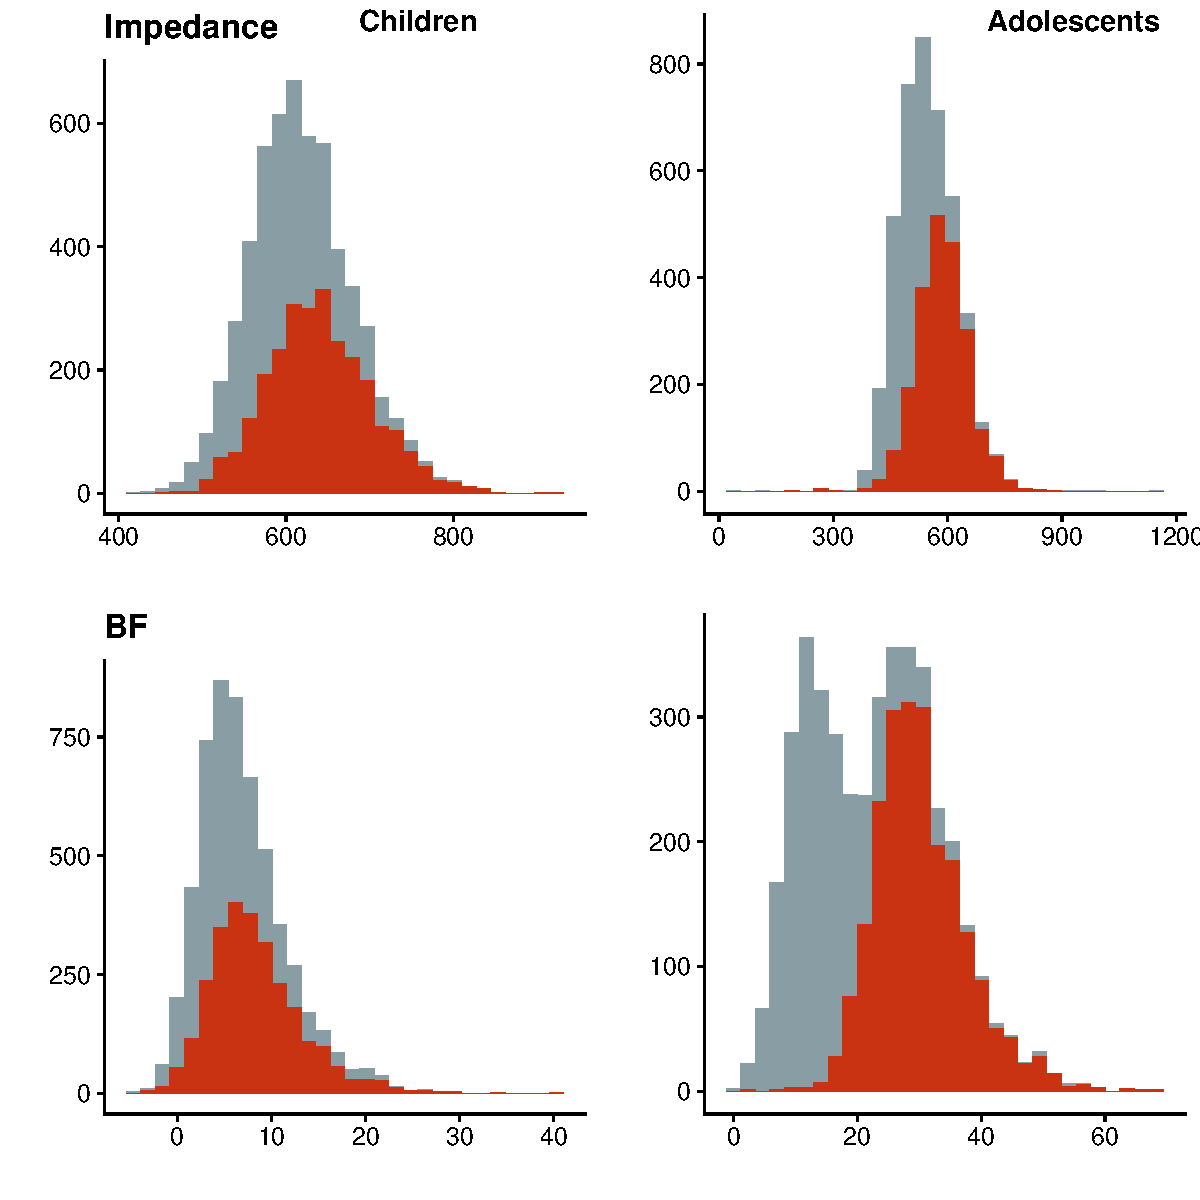
\includegraphics[width=1\linewidth]{data/observational/figures/bf_validation_histogram} 

}

\caption[Distribution of raw impedance and calculated body fat percentage in children and adolescents]{\textbf{Distribution of raw impedance and calculated body fat percentage in children and adolescents}. Plots give the distribution of the raw impedance value measured in ohms and body fat percentage (BF) derived using equation \eqref{eq:BF} for children and adolescents. Data is presented for complete cases across: raw metabolomics, body mass index, waist hip ratio (children only), impedance, height, weight, age, sex, and BF derived by impedance and dual energy x-ray absorptiometry in adolescents. Red is female data, grey is male data.}\label{fig:appendix-observational-figure-BF-validation-distribution}
\end{figure}



\begin{figure}

{\centering 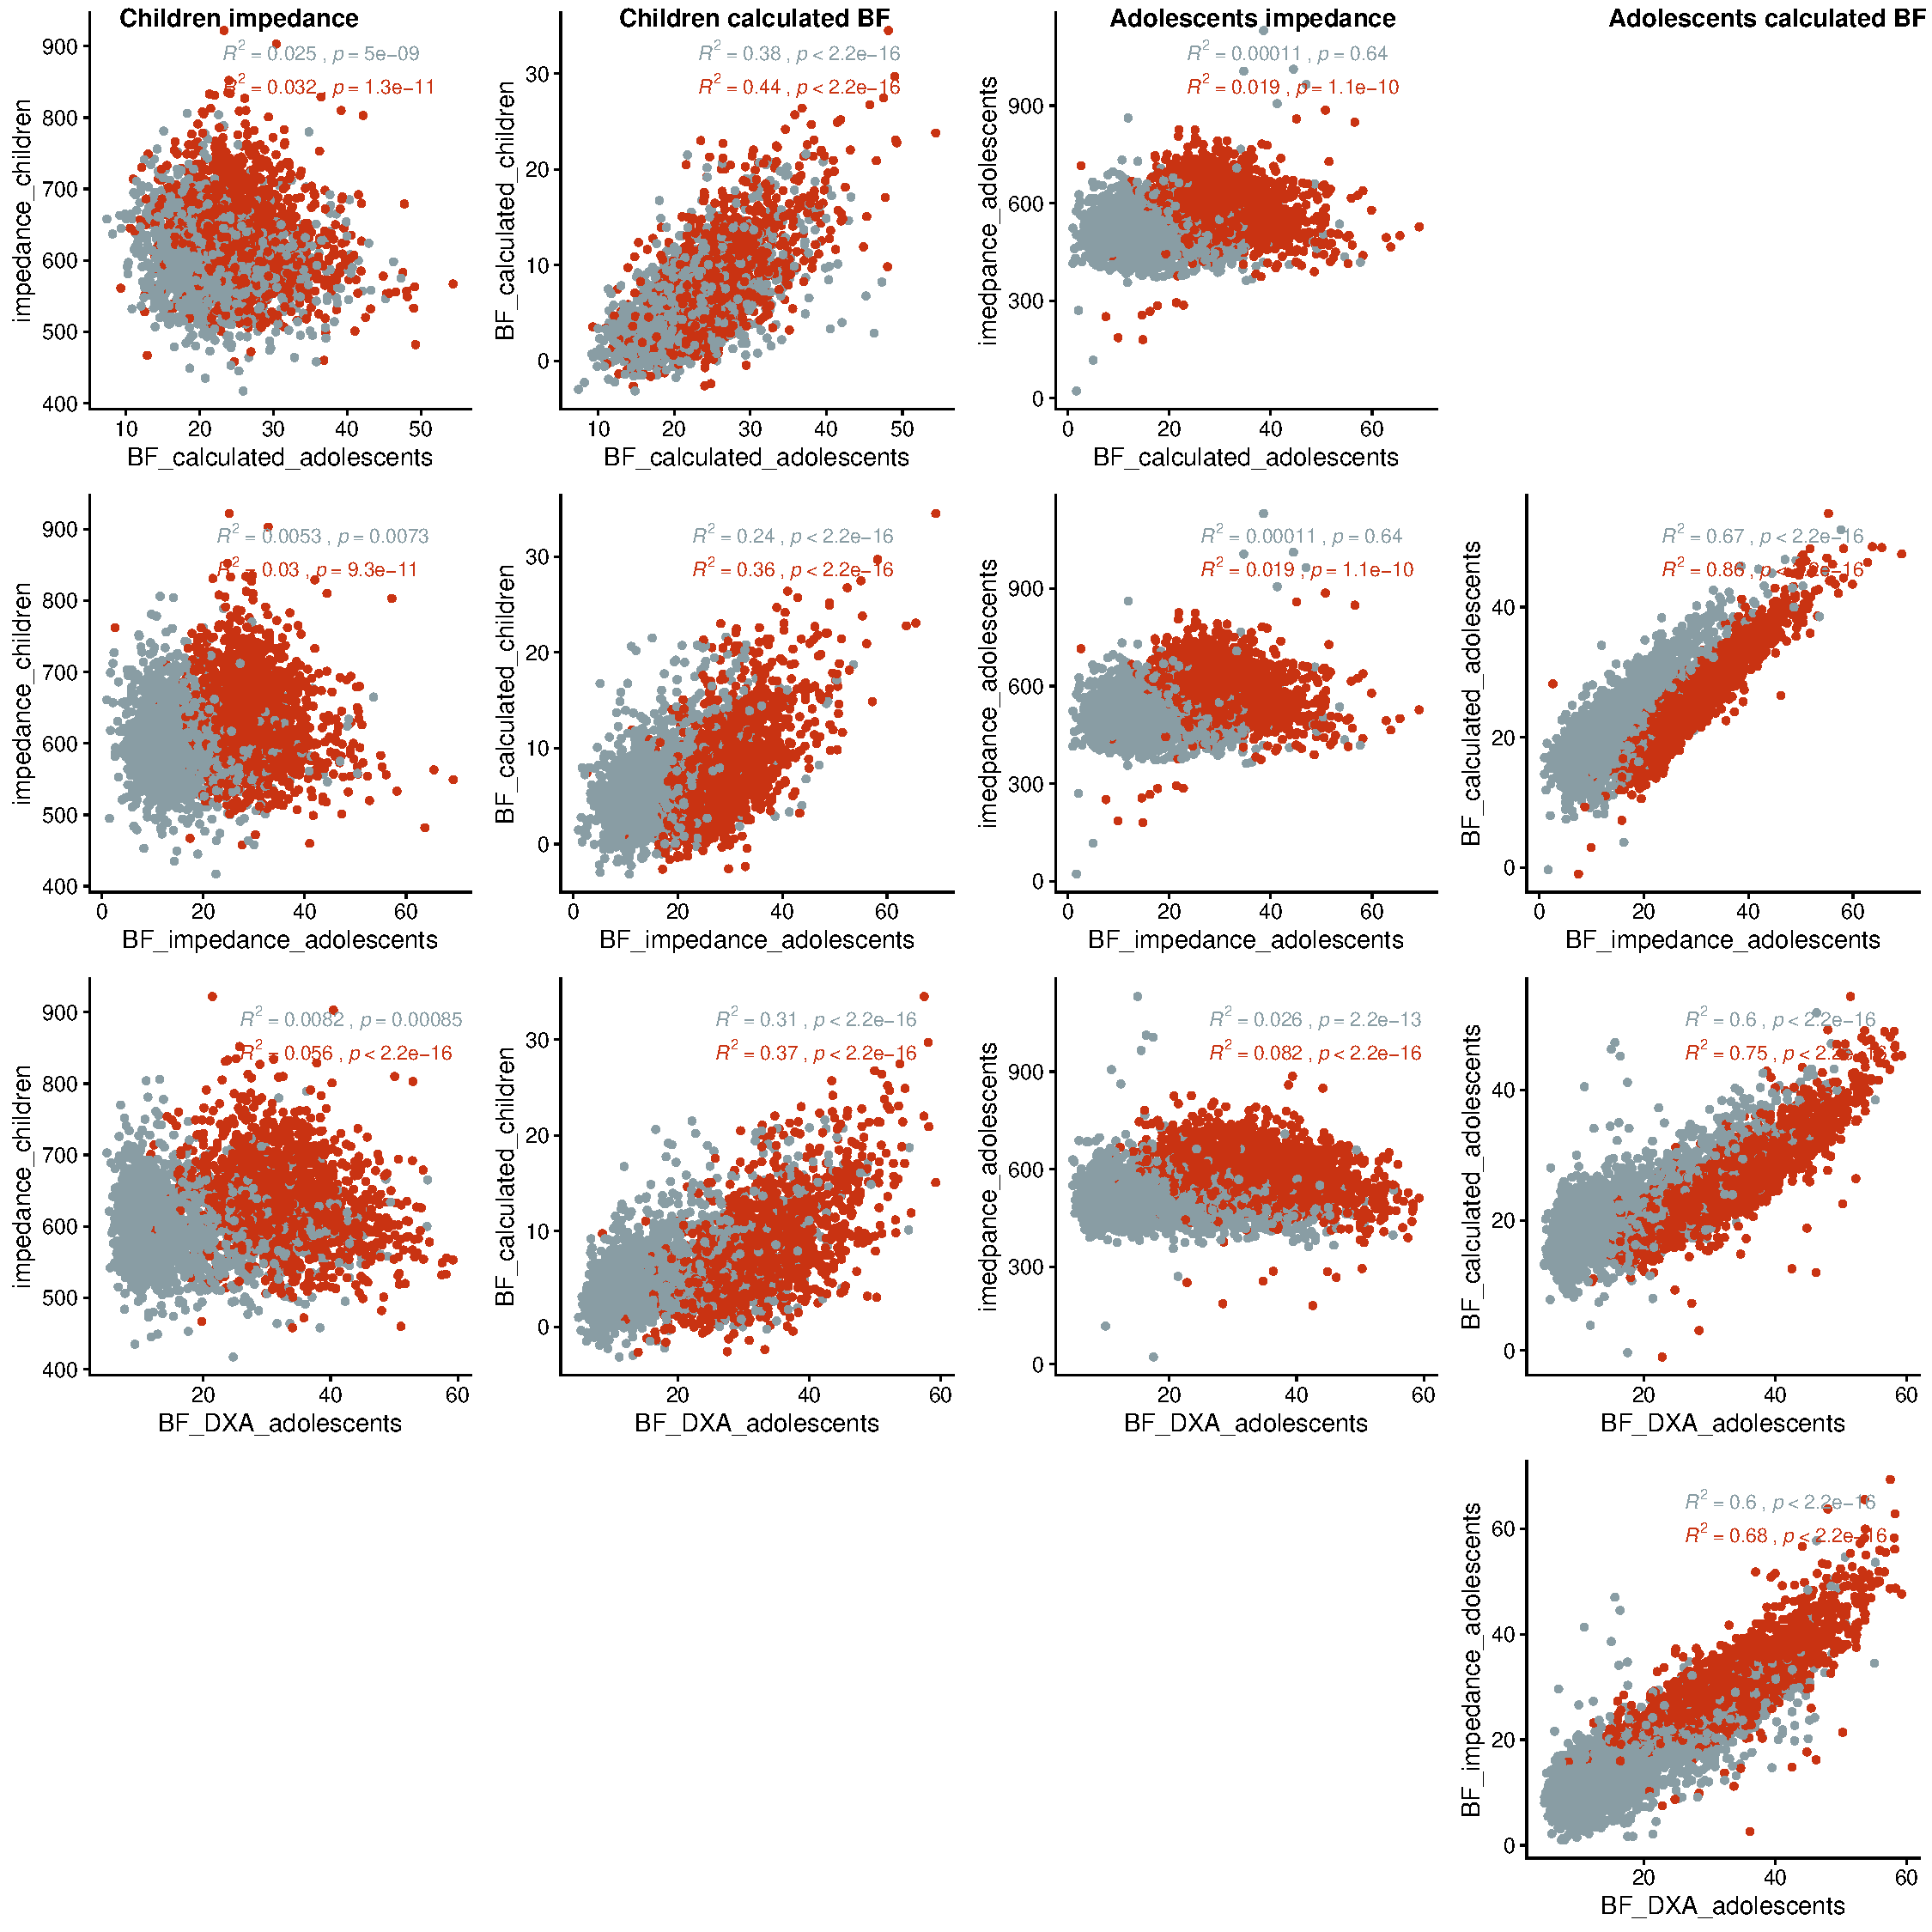
\includegraphics[width=1\linewidth]{data/observational/figures/bf_validation_correlation_bf} 

}

\caption[Correlation between different body fat percentage measures in children and adolescents]{\textbf{Correlation between different body fat percentage measures in children and adolescents}. Scatter plots are presented alongside Pearson's correlation coefficients for each sex; data for males are in grey and females in red. Plots are arranged in 4 columns and 4 rows. Column 1 gives raw impedance value in children (y axis) with body fat percentage (BF)-calculated in children and adolescents using equation \eqref{eq:BF}, and BF derived from dual energy x-ray absorptiometry (DXA) in adolescents. Column 2 gives child-calculated BF using equation \eqref{eq:BF} (y axis) with adolescent-calculated BF using equation \eqref{eq:BF} and DXA-derived BF. Column 3 gives adolescent raw impedance (y axis) with adolescent BF-calculated using equation \eqref{eq:BF} and DXA-derived BF. Column 4 gives adolescent calculated BF using equation \eqref{eq:BF} with adolescent raw impedance, DXA-derived BF, and adolescent raw impedance with DXA-derived BF. Data is presented for complete cases across: raw metabolomics, body mass index, waist hip ratio (children only), impedance, height, weight, age, sex, and BF derived by impedance and DXA in adolescents. Available on \href{https://github.com/mattlee821/000_thesis/blob/master/index/data/observational/figures/bf_validation_correlation_bf.pdf}{GitHub}.}\label{fig:appendix-observational-figure-BF-validation-correlation}
\end{figure}



\begin{figure}

{\centering 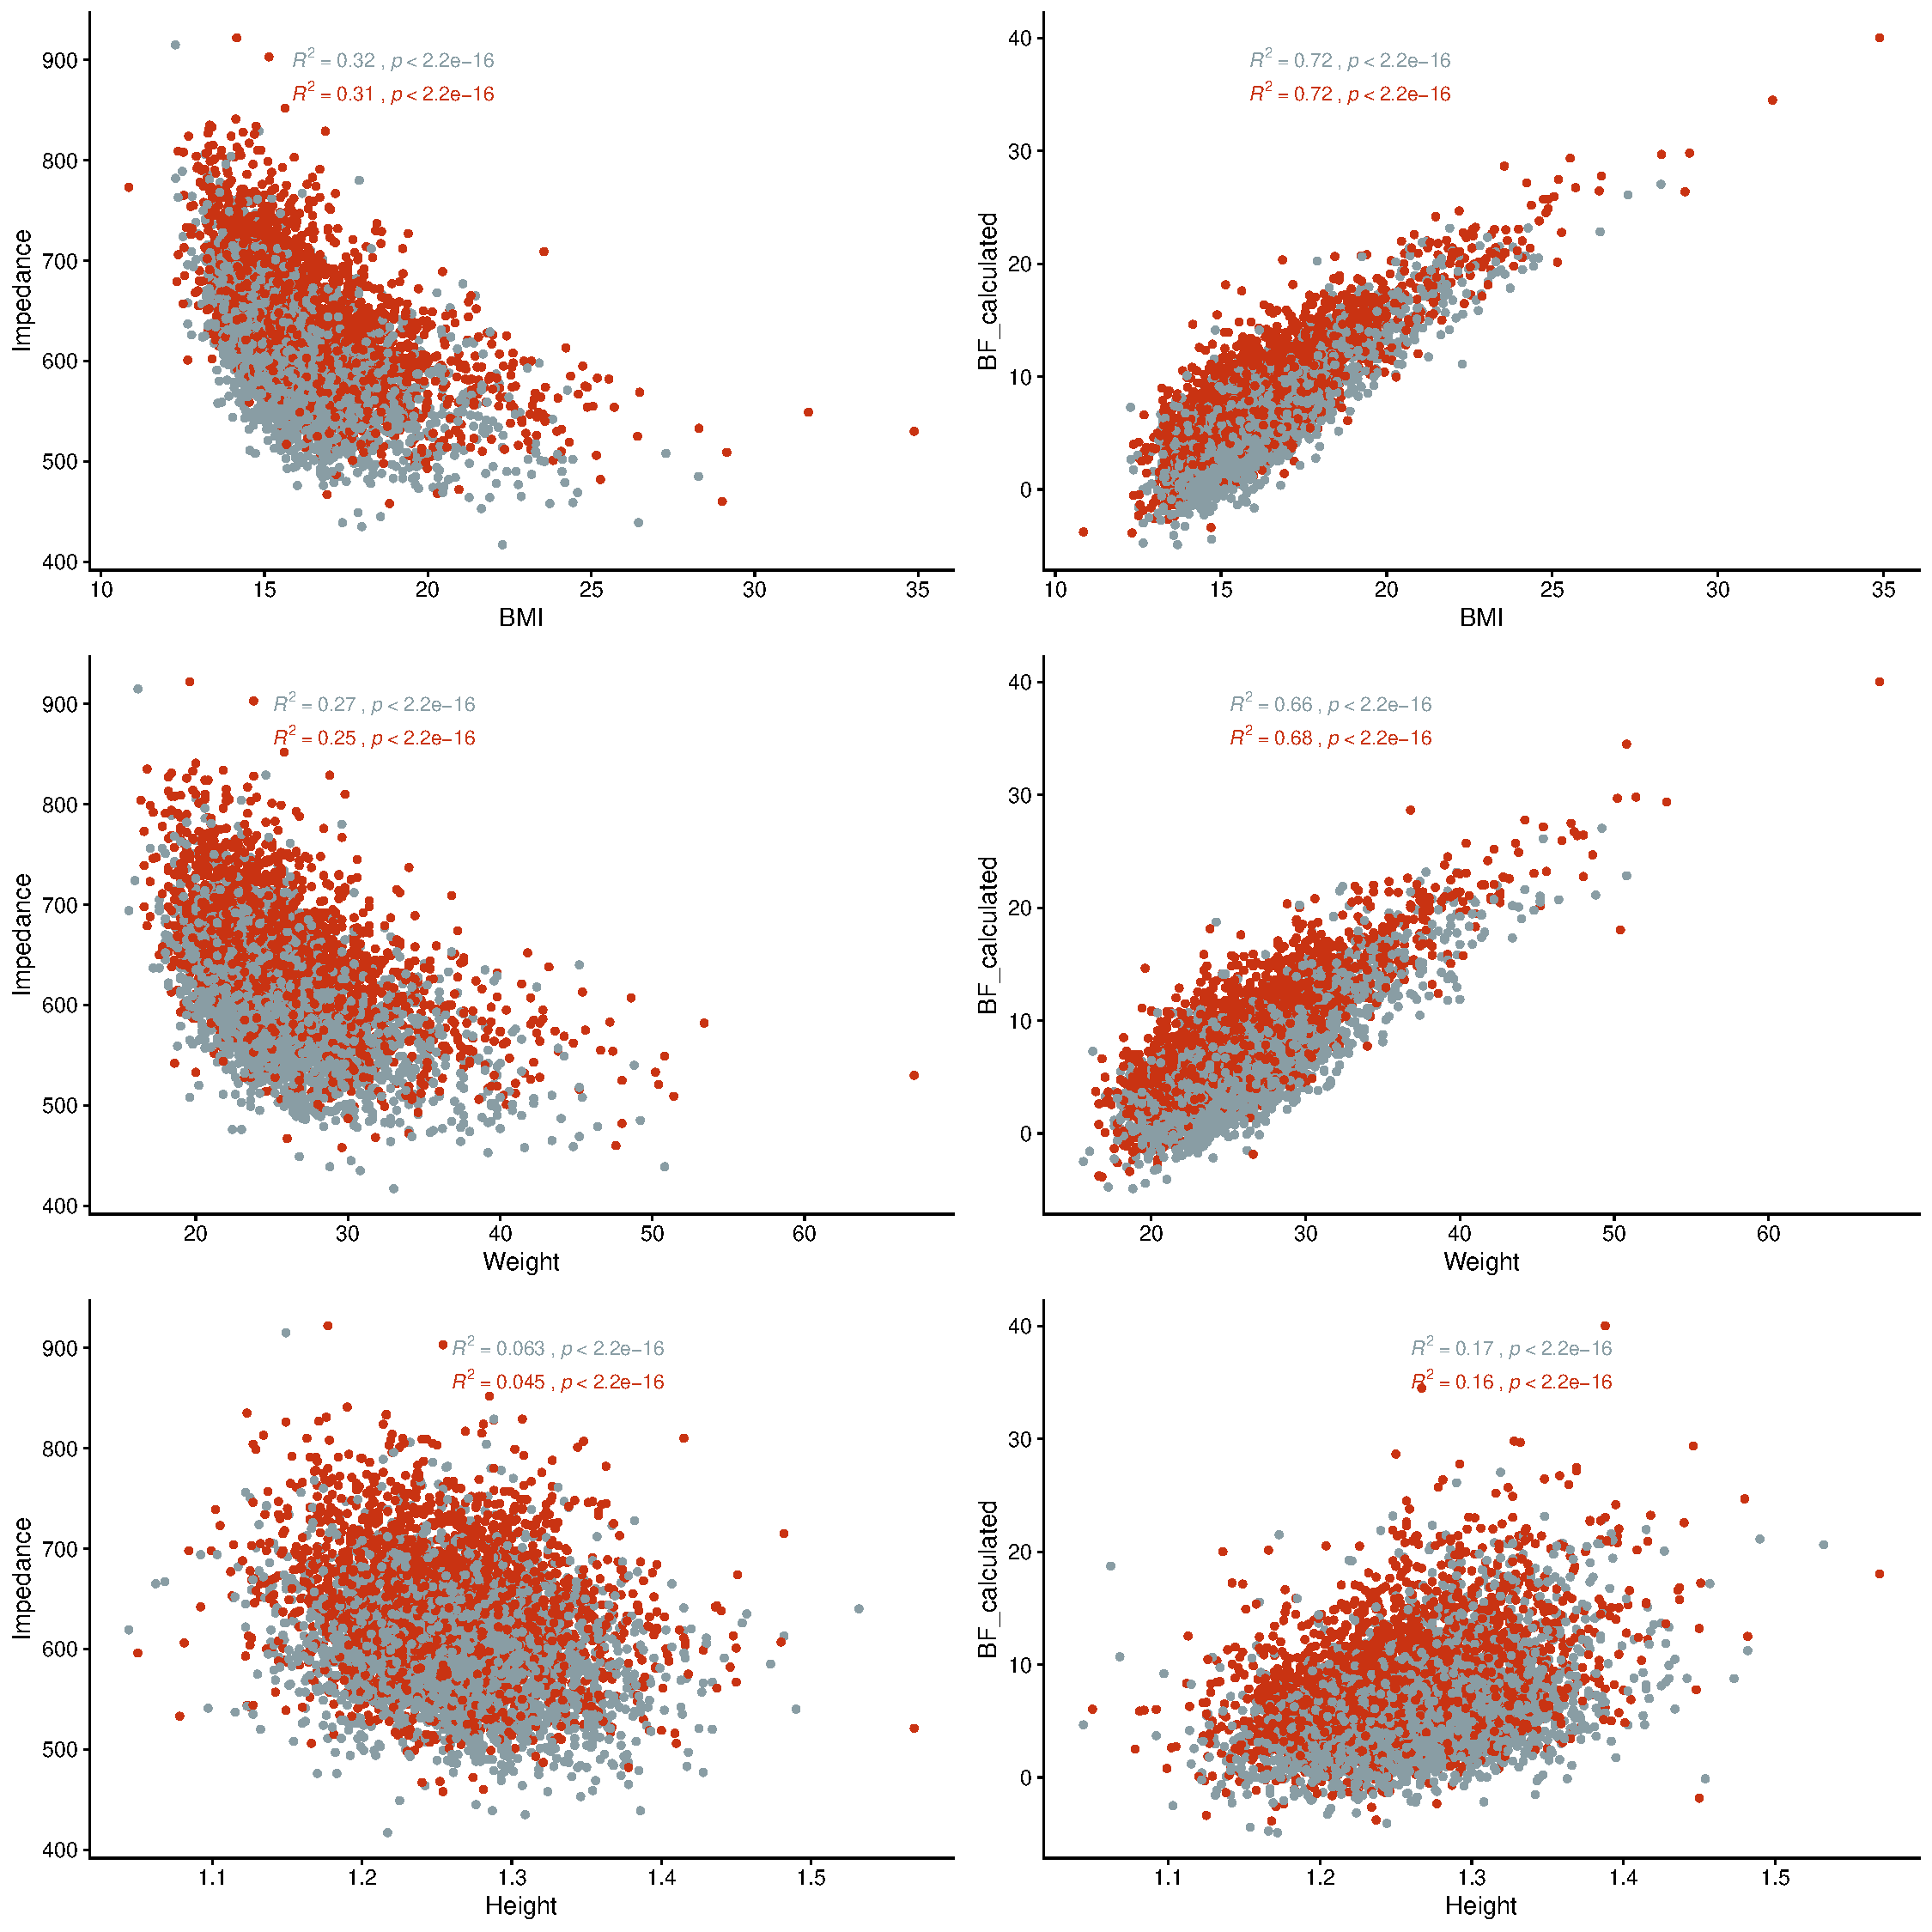
\includegraphics[width=1\linewidth]{data/observational/figures/bf_validation_correlation_children} 

}

\caption[Correlation between body fat percentage and anthropometric measures in children and adolescents]{\textbf{Correlation between body fat percentage and anthropometric measures in children.} Scatter plots are presented alongside Pearson's correlation coefficients for each sex; data for males are in grey and females in red. Column 1 = impedance; column 2 = body fat percentage (BF). Impedance is given as ohms. Data is presented for complete cases across: QC'd metabolomics, body mass index, waist hip ratio (children only), impedance, height, weight, age, sex, and BF derived by impedance and DXA in adolescents. Available on \href{https://github.com/mattlee821/000_thesis/blob/master/index/data/observational/figures/bf_validation_correlation_children.pdf}{GitHub}.}\label{fig:appendix-observational-figure-BF-validation-correlation-2-children}
\end{figure}



\begin{figure}

{\centering 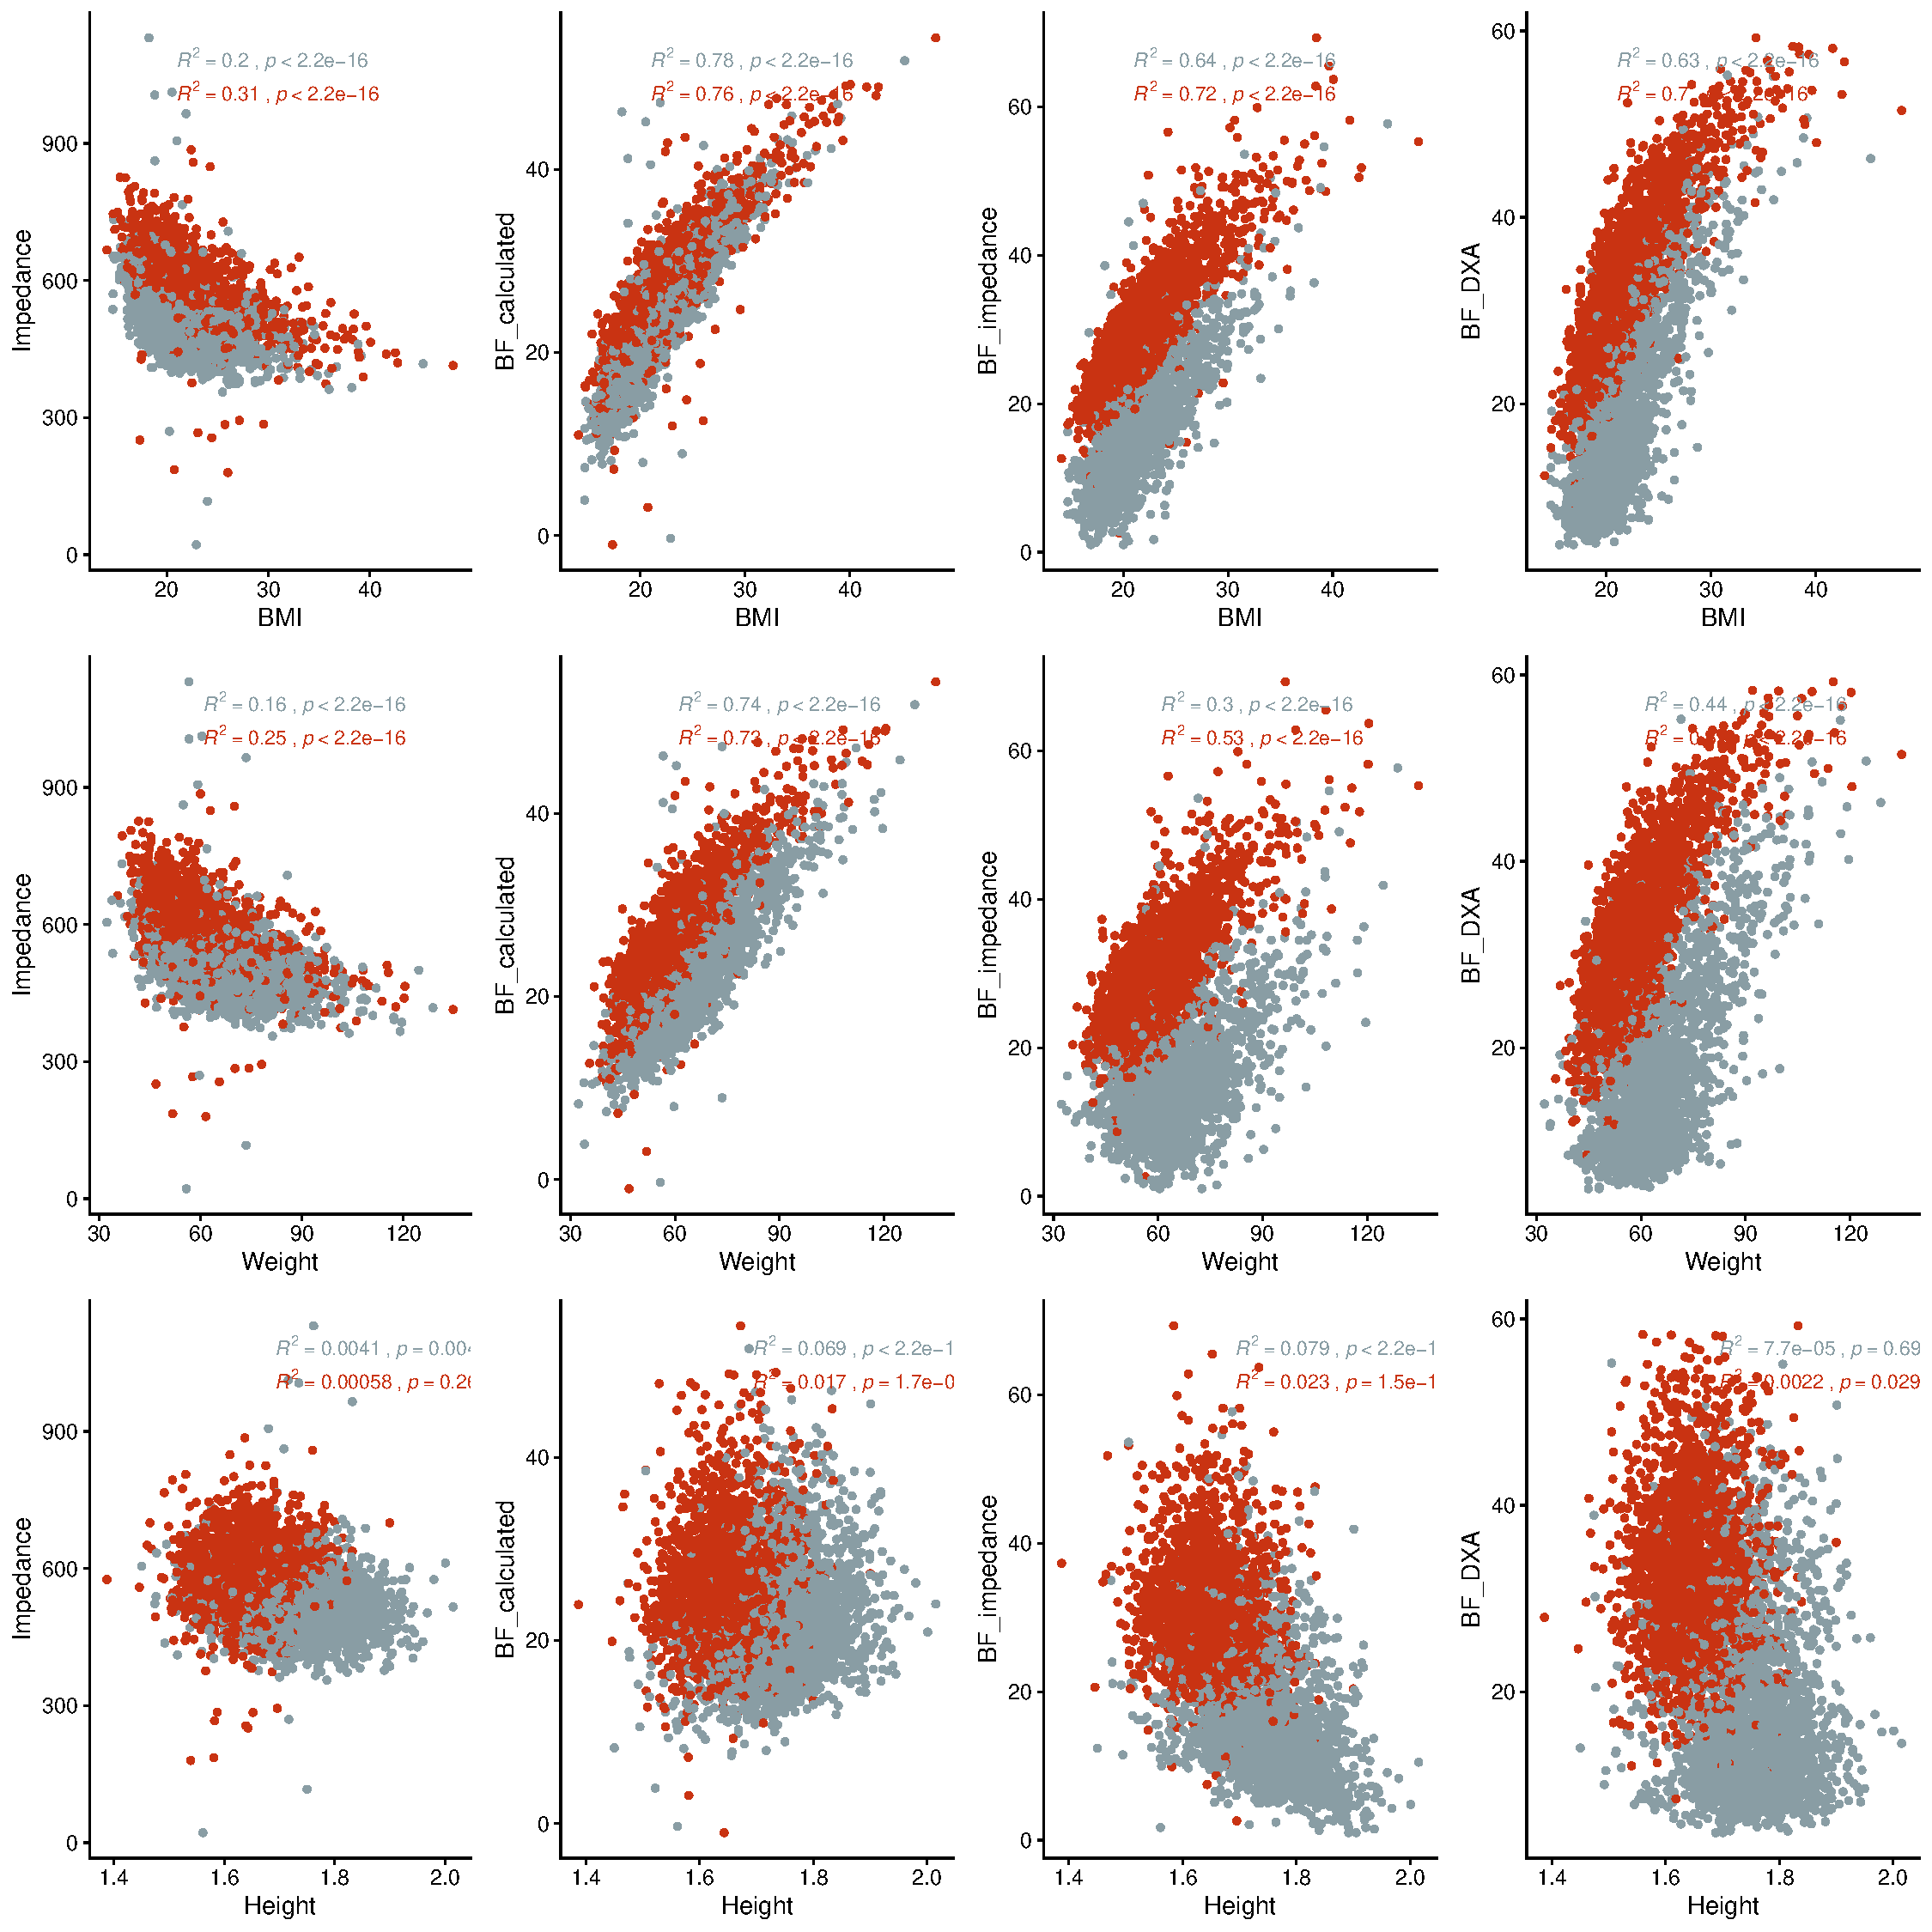
\includegraphics[width=1\linewidth]{data/observational/figures/bf_validation_correlation_adolescents} 

}

\caption[Correlation between body fat percentage and anthropometric measures in adolescents]{\textbf{Correlation between body fat percentage and anthropometric measures in adolescents.} Scatter plots are presented alongside Pearson's correlation coefficients for each sex; data for males are in grey and females in red. Column 1 = impedance; column 2 = BF calculated using equation \eqref{eq:BF}; column 3 = BF derived from impedance device; column 4 = BF derived from dual energy x-ray absorptiometry (DXA). Impedance is given as ohms. Data is presented for complete cases across: QC'd metabolomics, body mass index, waist hip ratio (children only), impedance, height, weight, age, sex, and BF derived by impedance and DXA in adolescents. Available on \href{https://github.com/mattlee821/000_thesis/blob/master/index/data/observational/figures/bf_validation_correlation_adolescents.pdf}{GitHub}.}\label{fig:appendix-observational-figure-BF-validation-correlation-2-adolescents}
\end{figure}
\newpage

\hypertarget{appendix-observational-metabolites}{%
\subsubsection{Metabolites}\label{appendix-observational-metabolites}}

\begingroup\fontsize{8}{10}\selectfont
\begin{ThreePartTable}
\begin{TableNotes}[para]
\item Metabolites are given with the originally measured units along with the Class and Subclass provided by the metabolomics platform and whether the metabolite is directly measured (no) or a derived metabolite measure.
\end{TableNotes}
\begin{longtabu} to \linewidth {>{\raggedright\arraybackslash}p{5em}>{\raggedright\arraybackslash}p{20em}>{\raggedright\arraybackslash}p{10em}>{\raggedright\arraybackslash}p{10em}>{\raggedright\arraybackslash}p{3em}}
\caption{\label{tab:appendix-observational-table-metabolites}List of metabolites available in the Avon Longitudinal Study of Parents and Children}\\
\toprule
Metabolite & Label & Class & Subclass & Derived\\
\midrule
\endfirsthead
\caption[]{\label{tab:appendix-observational-table-metabolites}List of metabolites available in the Avon Longitudinal Study of Parents and Children \textit{(continued)}}\\
\toprule
Metabolite & Label & Class & Subclass & Derived\\
\midrule
\endhead

\endfoot
\bottomrule
\insertTableNotes
\endlastfoot
\cellcolor{gray!6}{ala} & \cellcolor{gray!6}{Alanine (mmol/l)} & \cellcolor{gray!6}{Amino acids} & \cellcolor{gray!6}{Amino acids} & \cellcolor{gray!6}{no}\\
gln & Glutamine (mmol/l) & Amino acids & Amino acids & no\\
\cellcolor{gray!6}{his} & \cellcolor{gray!6}{Histidine (mmol/l)} & \cellcolor{gray!6}{Amino acids} & \cellcolor{gray!6}{Amino acids} & \cellcolor{gray!6}{no}\\
apoa1 & Apolipoprotein A-I (g/l) & Apolipoproteins & Apolipoproteins & no\\
\cellcolor{gray!6}{apob} & \cellcolor{gray!6}{Apolipoprotein B (g/l)} & \cellcolor{gray!6}{Apolipoproteins} & \cellcolor{gray!6}{Apolipoproteins} & \cellcolor{gray!6}{no}\\
\addlinespace
apobapoa1 & Ratio of apolipoprotein B to apolipoprotein A-I & Apolipoproteins & Apolipoproteins & no\\
\cellcolor{gray!6}{phe} & \cellcolor{gray!6}{Phenylalanine (mmol/l)} & \cellcolor{gray!6}{Amino acids} & \cellcolor{gray!6}{Aromatic amino acids} & \cellcolor{gray!6}{no}\\
tyr & Tyrosine (mmol/l) & Amino acids & Aromatic amino acids & no\\
\cellcolor{gray!6}{ile} & \cellcolor{gray!6}{Isoleucine (mmol/l)} & \cellcolor{gray!6}{Amino acids} & \cellcolor{gray!6}{Branched-chain amino acids} & \cellcolor{gray!6}{no}\\
leu & Leucine (mmol/l) & Amino acids & Branched-chain amino acids & no\\
\addlinespace
\cellcolor{gray!6}{val} & \cellcolor{gray!6}{Valine (mmol/l)} & \cellcolor{gray!6}{Amino acids} & \cellcolor{gray!6}{Branched-chain amino acids} & \cellcolor{gray!6}{no}\\
estc & Esterified cholesterol (mmol/l) & Cholesterol & Cholesterol & no\\
\cellcolor{gray!6}{freec} & \cellcolor{gray!6}{Free cholesterol (mmol/l)} & \cellcolor{gray!6}{Cholesterol} & \cellcolor{gray!6}{Cholesterol} & \cellcolor{gray!6}{no}\\
remnantc & Remnant cholesterol (non-HDL, non-LDL -cholesterol) (mmol/l) & Cholesterol & Cholesterol & no\\
\cellcolor{gray!6}{serumc} & \cellcolor{gray!6}{Serum total cholesterol (mmol/l)} & \cellcolor{gray!6}{Cholesterol} & \cellcolor{gray!6}{Cholesterol} & \cellcolor{gray!6}{no}\\
\addlinespace
hdlc & Total cholesterol in HDL (mmol/l) & Cholesterol & Cholesterol & no\\
\cellcolor{gray!6}{hdl2c} & \cellcolor{gray!6}{Total cholesterol in HDL2 (mmol/l)} & \cellcolor{gray!6}{Cholesterol} & \cellcolor{gray!6}{Cholesterol} & \cellcolor{gray!6}{no}\\
hdl3c & Total cholesterol in HDL3 (mmol/l) & Cholesterol & Cholesterol & no\\
\cellcolor{gray!6}{ldlc} & \cellcolor{gray!6}{Total cholesterol in LDL (mmol/l)} & \cellcolor{gray!6}{Cholesterol} & \cellcolor{gray!6}{Cholesterol} & \cellcolor{gray!6}{no}\\
vldlc & Total cholesterol in VLDL (mmol/l) & Cholesterol & Cholesterol & no\\
\addlinespace
\cellcolor{gray!6}{xxlvldlce} & \cellcolor{gray!6}{Cholesterol esters in chylomicrons and extremely large VLDL (mmol/l)} & \cellcolor{gray!6}{Lipoprotein subclasses} & \cellcolor{gray!6}{Extremely large VLDL} & \cellcolor{gray!6}{no}\\
xxlvldlp & Concentration of chylomicrons and extremely large VLDL particles (mol/l) & Lipoprotein subclasses & Extremely large VLDL & no\\
\cellcolor{gray!6}{xxlvldlfc} & \cellcolor{gray!6}{Free cholesterol in chylomicrons and extremely large VLDL (mmol/l)} & \cellcolor{gray!6}{Lipoprotein subclasses} & \cellcolor{gray!6}{Extremely large VLDL} & \cellcolor{gray!6}{no}\\
xxlvldlpl & Phospholipids in chylomicrons and extremely large VLDL (mmol/l) & Lipoprotein subclasses & Extremely large VLDL & no\\
\cellcolor{gray!6}{xxlvldlc} & \cellcolor{gray!6}{Total cholesterol in chylomicrons and extremely large VLDL (mmol/l)} & \cellcolor{gray!6}{Lipoprotein subclasses} & \cellcolor{gray!6}{Extremely large VLDL} & \cellcolor{gray!6}{no}\\
\addlinespace
xxlvldll & Total lipids in chylomicrons and extremely large VLDL (mmol/l) & Lipoprotein subclasses & Extremely large VLDL & no\\
\cellcolor{gray!6}{xxlvldltg} & \cellcolor{gray!6}{Triglycerides in chylomicrons and extremely large VLDL (mmol/l)} & \cellcolor{gray!6}{Lipoprotein subclasses} & \cellcolor{gray!6}{Extremely large VLDL} & \cellcolor{gray!6}{no}\\
xxlvldlcepct & Cholesterol esters in chylomicrons and extremely large VLDL to total lipids in chylomicrons and extremely large VLDL ratio (\%) & Lipoprotein subclasses ratios & Extremely large VLDL ratios & yes\\
\cellcolor{gray!6}{xxlvldlfcpct} & \cellcolor{gray!6}{Free cholesterol in chylomicrons and extremely large VLDL to total lipids in chylomicrons and extremely large VLDL ratio (\%)} & \cellcolor{gray!6}{Lipoprotein subclasses ratios} & \cellcolor{gray!6}{Extremely large VLDL ratios} & \cellcolor{gray!6}{yes}\\
xxlvldlplpct & Phospholipids in chylomicrons and extremely large VLDL to total lipids in chylomicrons and extremely large VLDL ratio (\%) & Lipoprotein subclasses ratios & Extremely large VLDL ratios & yes\\
\addlinespace
\cellcolor{gray!6}{xxlvldlcpct} & \cellcolor{gray!6}{Total cholesterol in chylomicrons and extremely large VLDL to total lipids in chylomicrons and extremely large VLDL ratio (\%)} & \cellcolor{gray!6}{Lipoprotein subclasses ratios} & \cellcolor{gray!6}{Extremely large VLDL ratios} & \cellcolor{gray!6}{yes}\\
xxlvldltgpct & Triglycerides in chylomicrons and extremely large VLDL to total lipids in chylomicrons and extremely large VLDL ratio (\%) & Lipoprotein subclasses ratios & Extremely large VLDL ratios & yes\\
\cellcolor{gray!6}{la} & \cellcolor{gray!6}{18:2, linoleic acid (mmol/l)} & \cellcolor{gray!6}{Fatty acids} & \cellcolor{gray!6}{Fatty acids} & \cellcolor{gray!6}{no}\\
dha & 22:6, docosahexaenoic acid (mmol/l) & Fatty acids & Fatty acids & no\\
\cellcolor{gray!6}{cla} & \cellcolor{gray!6}{Conjugated linoleic acid (mmol/l)} & \cellcolor{gray!6}{Fatty acids} & \cellcolor{gray!6}{Fatty acids} & \cellcolor{gray!6}{no}\\
\addlinespace
unsat & Estimated degree of unsaturation & Fatty acids & Fatty acids & no\\
\cellcolor{gray!6}{unsatdeg} & \cellcolor{gray!6}{Estimated degree of unsaturation} & \cellcolor{gray!6}{Fatty acids} & \cellcolor{gray!6}{Fatty acids} & \cellcolor{gray!6}{yes}\\
falen & Estimated description of fatty acid chain length, not actual carbon number & Fatty acids & Fatty acids & no\\
\cellcolor{gray!6}{mufa} & \cellcolor{gray!6}{Monounsaturated fatty acids; 16:1, 18:1 (mmol/l)} & \cellcolor{gray!6}{Fatty acids} & \cellcolor{gray!6}{Fatty acids} & \cellcolor{gray!6}{no}\\
faw3 & Omega-3 fatty acids (mmol/l) & Fatty acids & Fatty acids & no\\
\addlinespace
\cellcolor{gray!6}{faw6} & \cellcolor{gray!6}{Omega-6 fatty acids (mmol/l)} & \cellcolor{gray!6}{Fatty acids} & \cellcolor{gray!6}{Fatty acids} & \cellcolor{gray!6}{no}\\
pufa & Polyunsaturated fatty acids (mmol/l) & Fatty acids & Fatty acids & no\\
\cellcolor{gray!6}{sfa} & \cellcolor{gray!6}{Saturated fatty acids (mmol/l)} & \cellcolor{gray!6}{Fatty acids} & \cellcolor{gray!6}{Fatty acids} & \cellcolor{gray!6}{no}\\
totfa & Total fatty acids (mmol/l) & Fatty acids & Fatty acids & no\\
\cellcolor{gray!6}{lafa} & \cellcolor{gray!6}{Ratio of 18:2 linoleic acid to total fatty acids (\%)} & \cellcolor{gray!6}{Fatty acids ratios} & \cellcolor{gray!6}{Fatty acids ratios} & \cellcolor{gray!6}{yes}\\
\addlinespace
dhafa & Ratio of 22:6 docosahexaenoic acid to total fatty acids (\%) & Fatty acids ratios & Fatty acids ratios & yes\\
\cellcolor{gray!6}{clafa} & \cellcolor{gray!6}{Ratio of conjugated linoleic acid to total fatty acids (\%)} & \cellcolor{gray!6}{Fatty acids ratios} & \cellcolor{gray!6}{Fatty acids ratios} & \cellcolor{gray!6}{yes}\\
mufafa & Ratio of monounsaturated fatty acids to total fatty acids (\%) & Fatty acids ratios & Fatty acids ratios & yes\\
\cellcolor{gray!6}{faw3fa} & \cellcolor{gray!6}{Ratio of omega-3 fatty acids to total fatty acids (\%)} & \cellcolor{gray!6}{Fatty acids ratios} & \cellcolor{gray!6}{Fatty acids ratios} & \cellcolor{gray!6}{yes}\\
faw6fa & Ratio of omega-6 fatty acids to total fatty acids (\%) & Fatty acids ratios & Fatty acids ratios & yes\\
\addlinespace
\cellcolor{gray!6}{pufafa} & \cellcolor{gray!6}{Ratio of polyunsaturated fatty acids to total fatty acids (\%)} & \cellcolor{gray!6}{Fatty acids ratios} & \cellcolor{gray!6}{Fatty acids ratios} & \cellcolor{gray!6}{yes}\\
sfafa & Ratio of saturated fatty acids to total fatty acids (\%) & Fatty acids ratios & Fatty acids ratios & yes\\
\cellcolor{gray!6}{alb} & \cellcolor{gray!6}{Albumin  (signal area)} & \cellcolor{gray!6}{Fluid balance} & \cellcolor{gray!6}{Fluid balance} & \cellcolor{gray!6}{no}\\
crea & Creatinine (mmol/l) & Fluid balance & Fluid balance & no\\
\cellcolor{gray!6}{dag} & \cellcolor{gray!6}{Diacylglycerol (mmol/l)} & \cellcolor{gray!6}{Glycerides and phospholipids} & \cellcolor{gray!6}{Glycerides and phospholipids} & \cellcolor{gray!6}{no}\\
\addlinespace
pc & Phosphatidylcholine and other cholines (mmol/l) & Glycerides and phospholipids & Glycerides and phospholipids & no\\
\cellcolor{gray!6}{serumtg} & \cellcolor{gray!6}{Serum total triglycerides (mmol/l)} & \cellcolor{gray!6}{Glycerides and phospholipids} & \cellcolor{gray!6}{Glycerides and phospholipids} & \cellcolor{gray!6}{no}\\
sm & Sphingomyelins (mmol/l) & Glycerides and phospholipids & Glycerides and phospholipids & no\\
\cellcolor{gray!6}{totcho} & \cellcolor{gray!6}{Total cholines (mmol/l)} & \cellcolor{gray!6}{Glycerides and phospholipids} & \cellcolor{gray!6}{Glycerides and phospholipids} & \cellcolor{gray!6}{no}\\
totpg & Total phosphoglycerides (mmol/l) & Glycerides and phospholipids & Glycerides and phospholipids & no\\
\addlinespace
\cellcolor{gray!6}{hdltg} & \cellcolor{gray!6}{Triglycerides in HDL (mmol/l)} & \cellcolor{gray!6}{Glycerides and phospholipids} & \cellcolor{gray!6}{Glycerides and phospholipids} & \cellcolor{gray!6}{no}\\
ldltg & Triglycerides in LDL (mmol/l) & Glycerides and phospholipids & Glycerides and phospholipids & no\\
\cellcolor{gray!6}{vldltg} & \cellcolor{gray!6}{Triglycerides in VLDL (mmol/l)} & \cellcolor{gray!6}{Glycerides and phospholipids} & \cellcolor{gray!6}{Glycerides and phospholipids} & \cellcolor{gray!6}{no}\\
dagtg & Ratio of diacylglycerol to triglycerides (\%) & Glycerides and phospholipids ratios & Glycerides and phospholipids ratios & yes\\
\cellcolor{gray!6}{tgpg} & \cellcolor{gray!6}{Ratio of triglycerides to phosphoglycerides ratio (\%)} & \cellcolor{gray!6}{Glycerides and phospholipids ratios} & \cellcolor{gray!6}{Glycerides and phospholipids ratios} & \cellcolor{gray!6}{yes}\\
\addlinespace
cit & Citrate (mmol/l) & Glycolysis related metabolites & Glycolysis related metabolites & no\\
\cellcolor{gray!6}{glc} & \cellcolor{gray!6}{Glucose (mmol/l)} & \cellcolor{gray!6}{Glycolysis related metabolites} & \cellcolor{gray!6}{Glycolysis related metabolites} & \cellcolor{gray!6}{no}\\
lac & Lactate (mmol/l) & Glycolysis related metabolites & Glycolysis related metabolites & no\\
\cellcolor{gray!6}{pyr} & \cellcolor{gray!6}{Pyruvate (mmol/l)} & \cellcolor{gray!6}{Glycolysis related metabolites} & \cellcolor{gray!6}{Glycolysis related metabolites} & \cellcolor{gray!6}{no}\\
idlce & Cholesterol esters in IDL (mmol/l) & Lipoprotein subclasses & IDL & no\\
\addlinespace
\cellcolor{gray!6}{idlp} & \cellcolor{gray!6}{Concentration of IDL particles (mol/l)} & \cellcolor{gray!6}{Lipoprotein subclasses} & \cellcolor{gray!6}{IDL} & \cellcolor{gray!6}{no}\\
idlfc & Free cholesterol in IDL (mmol/l) & Lipoprotein subclasses & IDL & no\\
\cellcolor{gray!6}{idlpl} & \cellcolor{gray!6}{Phospholipids in IDL (mmol/l)} & \cellcolor{gray!6}{Lipoprotein subclasses} & \cellcolor{gray!6}{IDL} & \cellcolor{gray!6}{no}\\
idlc & Total cholesterol in IDL (mmol/l) & Lipoprotein subclasses & IDL & no\\
\cellcolor{gray!6}{idll} & \cellcolor{gray!6}{Total lipids in IDL (mmol/l)} & \cellcolor{gray!6}{Lipoprotein subclasses} & \cellcolor{gray!6}{IDL} & \cellcolor{gray!6}{no}\\
\addlinespace
idltg & Triglycerides in IDL (mmol/l) & Lipoprotein subclasses & IDL & no\\
\cellcolor{gray!6}{idlcepct} & \cellcolor{gray!6}{Cholesterol esters in IDL to total lipids in IDL ratio (\%)} & \cellcolor{gray!6}{Lipoprotein subclasses ratios} & \cellcolor{gray!6}{IDL ratios} & \cellcolor{gray!6}{yes}\\
idlfcpct & Free cholesterol in IDL to total lipids in IDL ratio (\%) & Lipoprotein subclasses ratios & IDL ratios & yes\\
\cellcolor{gray!6}{idlplpct} & \cellcolor{gray!6}{Phospholipids in IDL to total lipids in IDL ratio (\%)} & \cellcolor{gray!6}{Lipoprotein subclasses ratios} & \cellcolor{gray!6}{IDL ratios} & \cellcolor{gray!6}{yes}\\
idlcpct & Total cholesterol in IDL to total lipids in IDL ratio (\%) & Lipoprotein subclasses ratios & IDL ratios & yes\\
\addlinespace
\cellcolor{gray!6}{idltgpct} & \cellcolor{gray!6}{Triglycerides in IDL to total lipids in IDL ratio (\%)} & \cellcolor{gray!6}{Lipoprotein subclasses ratios} & \cellcolor{gray!6}{IDL ratios} & \cellcolor{gray!6}{yes}\\
gp & Glycoprotein acetyls, mainly a1-acid glycoprotein (mmol/l) & Inflammation & Inflammation & no\\
\cellcolor{gray!6}{bohbut} & \cellcolor{gray!6}{3-hydroxybutyrate (mmol/l)} & \cellcolor{gray!6}{Ketone bodies} & \cellcolor{gray!6}{Ketone bodies} & \cellcolor{gray!6}{no}\\
ace & Acetate (mmol/l) & Ketone bodies & Ketone bodies & no\\
\cellcolor{gray!6}{acace} & \cellcolor{gray!6}{Acetoacetate (mmol/l)} & \cellcolor{gray!6}{Ketone bodies} & \cellcolor{gray!6}{Ketone bodies} & \cellcolor{gray!6}{no}\\
\addlinespace
lhdlce & Cholesterol esters in large HDL (mmol/l) & Lipoprotein subclasses & Large HDL & no\\
\cellcolor{gray!6}{lhdlp} & \cellcolor{gray!6}{Concentration of large HDL particles (mol/l)} & \cellcolor{gray!6}{Lipoprotein subclasses} & \cellcolor{gray!6}{Large HDL} & \cellcolor{gray!6}{no}\\
lhdlfc & Free cholesterol in large HDL (mmol/l) & Lipoprotein subclasses & Large HDL & no\\
\cellcolor{gray!6}{lhdlpl} & \cellcolor{gray!6}{Phospholipids in large HDL (mmol/l)} & \cellcolor{gray!6}{Lipoprotein subclasses} & \cellcolor{gray!6}{Large HDL} & \cellcolor{gray!6}{no}\\
lhdlc & Total cholesterol in large HDL (mmol/l) & Lipoprotein subclasses & Large HDL & no\\
\addlinespace
\cellcolor{gray!6}{lhdll} & \cellcolor{gray!6}{Total lipids in large HDL (mmol/l)} & \cellcolor{gray!6}{Lipoprotein subclasses} & \cellcolor{gray!6}{Large HDL} & \cellcolor{gray!6}{no}\\
lhdltg & Triglycerides in large HDL (mmol/l) & Lipoprotein subclasses & Large HDL & no\\
\cellcolor{gray!6}{lhdlcepct} & \cellcolor{gray!6}{Cholesterol esters in large HDL to total lipids in large HDL ratio (\%)} & \cellcolor{gray!6}{Lipoprotein subclasses ratios} & \cellcolor{gray!6}{Large HDL ratios} & \cellcolor{gray!6}{yes}\\
lhdlfcpct & Free cholesterol in large HDL to total lipids in large HDL ratio (\%) & Lipoprotein subclasses ratios & Large HDL ratios & yes\\
\cellcolor{gray!6}{lhdlplpct} & \cellcolor{gray!6}{Phospholipids in large HDL to total lipids in large HDL ratio (\%)} & \cellcolor{gray!6}{Lipoprotein subclasses ratios} & \cellcolor{gray!6}{Large HDL ratios} & \cellcolor{gray!6}{yes}\\
\addlinespace
lhdlcpct & Total cholesterol in large HDL to total lipids in large HDL ratio (\%) & Lipoprotein subclasses ratios & Large HDL ratios & yes\\
\cellcolor{gray!6}{lhdltgpct} & \cellcolor{gray!6}{Triglycerides in large HDL to total lipids in large HDL ratio (\%)} & \cellcolor{gray!6}{Lipoprotein subclasses ratios} & \cellcolor{gray!6}{Large HDL ratios} & \cellcolor{gray!6}{yes}\\
lldlce & Cholesterol esters in large LDL (mmol/l) & Lipoprotein subclasses & Large LDL & no\\
\cellcolor{gray!6}{lldlp} & \cellcolor{gray!6}{Concentration of large LDL particles (mol/l)} & \cellcolor{gray!6}{Lipoprotein subclasses} & \cellcolor{gray!6}{Large LDL} & \cellcolor{gray!6}{no}\\
lldlfc & Free cholesterol in large LDL (mmol/l) & Lipoprotein subclasses & Large LDL & no\\
\addlinespace
\cellcolor{gray!6}{lldlpl} & \cellcolor{gray!6}{Phospholipids in large LDL (mmol/l)} & \cellcolor{gray!6}{Lipoprotein subclasses} & \cellcolor{gray!6}{Large LDL} & \cellcolor{gray!6}{no}\\
lldlc & Total cholesterol in large LDL (mmol/l) & Lipoprotein subclasses & Large LDL & no\\
\cellcolor{gray!6}{lldll} & \cellcolor{gray!6}{Total lipids in large LDL (mmol/l)} & \cellcolor{gray!6}{Lipoprotein subclasses} & \cellcolor{gray!6}{Large LDL} & \cellcolor{gray!6}{no}\\
lldltg & Triglycerides in large LDL (mmol/l) & Lipoprotein subclasses & Large LDL & no\\
\cellcolor{gray!6}{lldlcepct} & \cellcolor{gray!6}{Cholesterol esters in large LDL to total lipids in large LDL ratio (\%)} & \cellcolor{gray!6}{Lipoprotein subclasses ratios} & \cellcolor{gray!6}{Large LDL ratios} & \cellcolor{gray!6}{yes}\\
\addlinespace
lldlcpct & Total cholesterol in large LDL to total lipids in large LDL ratio (\%) & Lipoprotein subclasses ratios & Large LDL ratios & yes\\
\cellcolor{gray!6}{lldlfcpct} & \cellcolor{gray!6}{Free cholesterol in large LDL to total lipids in large LDL ratio (\%)} & \cellcolor{gray!6}{Lipoprotein subclasses ratios} & \cellcolor{gray!6}{Large LDL ratios} & \cellcolor{gray!6}{yes}\\
lldlplpct & Phospholipids in large LDL to total lipids in large LDL ratio (\%) & Lipoprotein subclasses ratios & Large LDL ratios & yes\\
\cellcolor{gray!6}{lldltgpct} & \cellcolor{gray!6}{Triglycerides in large LDL to total lipids in large LDL ratio (\%)} & \cellcolor{gray!6}{Lipoprotein subclasses ratios} & \cellcolor{gray!6}{Large LDL ratios} & \cellcolor{gray!6}{yes}\\
lvldlce & Cholesterol esters in large VLDL (mmol/l) & Lipoprotein subclasses & Large VLDL & no\\
\addlinespace
\cellcolor{gray!6}{lvldlp} & \cellcolor{gray!6}{Concentration of large VLDL particles (mol/l)} & \cellcolor{gray!6}{Lipoprotein subclasses} & \cellcolor{gray!6}{Large VLDL} & \cellcolor{gray!6}{no}\\
lvldlfc & Free cholesterol in large VLDL (mmol/l) & Lipoprotein subclasses & Large VLDL & no\\
\cellcolor{gray!6}{lvldlpl} & \cellcolor{gray!6}{Phospholipids in large VLDL (mmol/l)} & \cellcolor{gray!6}{Lipoprotein subclasses} & \cellcolor{gray!6}{Large VLDL} & \cellcolor{gray!6}{no}\\
lvldlc & Total cholesterol in large VLDL (mmol/l) & Lipoprotein subclasses & Large VLDL & no\\
\cellcolor{gray!6}{lvldll} & \cellcolor{gray!6}{Total lipids in large VLDL (mmol/l)} & \cellcolor{gray!6}{Lipoprotein subclasses} & \cellcolor{gray!6}{Large VLDL} & \cellcolor{gray!6}{no}\\
\addlinespace
lvldltg & Triglycerides in large VLDL (mmol/l) & Lipoprotein subclasses & Large VLDL & no\\
\cellcolor{gray!6}{lvldlcepct} & \cellcolor{gray!6}{Cholesterol esters in large VLDL to total lipids in large VLDL ratio (\%)} & \cellcolor{gray!6}{Lipoprotein subclasses ratios} & \cellcolor{gray!6}{Large VLDL ratios} & \cellcolor{gray!6}{yes}\\
lvldlfcpct & Free cholesterol in large VLDL to total lipids in large VLDL ratio (\%) & Lipoprotein subclasses ratios & Large VLDL ratios & yes\\
\cellcolor{gray!6}{lvldlplpct} & \cellcolor{gray!6}{Phospholipids in large VLDL to total lipids in large VLDL ratio (\%)} & \cellcolor{gray!6}{Lipoprotein subclasses ratios} & \cellcolor{gray!6}{Large VLDL ratios} & \cellcolor{gray!6}{yes}\\
lvldlcpct & Total cholesterol in large VLDL to total lipids in large VLDL ratio (\%) & Lipoprotein subclasses ratios & Large VLDL ratios & yes\\
\addlinespace
\cellcolor{gray!6}{lvldltgpct} & \cellcolor{gray!6}{Triglycerides in large VLDL to total lipids in large VLDL ratio (\%)} & \cellcolor{gray!6}{Lipoprotein subclasses ratios} & \cellcolor{gray!6}{Large VLDL ratios} & \cellcolor{gray!6}{yes}\\
hdld & Mean diameter for HDL particles (nm) & Lipoprotein particle size & Lipoprotein particle size & no\\
\cellcolor{gray!6}{ldld} & \cellcolor{gray!6}{Mean diameter for LDL particles (nm)} & \cellcolor{gray!6}{Lipoprotein particle size} & \cellcolor{gray!6}{Lipoprotein particle size} & \cellcolor{gray!6}{no}\\
vldld & Mean diameter for VLDL particles (nm) & Lipoprotein particle size & Lipoprotein particle size & no\\
\cellcolor{gray!6}{mhdlce} & \cellcolor{gray!6}{Cholesterol esters in medium HDL (mmol/l)} & \cellcolor{gray!6}{Lipoprotein subclasses} & \cellcolor{gray!6}{Medium HDL} & \cellcolor{gray!6}{no}\\
\addlinespace
mhdlp & Concentration of medium HDL particles (mol/l) & Lipoprotein subclasses & Medium HDL & no\\
\cellcolor{gray!6}{mhdlfc} & \cellcolor{gray!6}{Free cholesterol in medium HDL (mmol/l)} & \cellcolor{gray!6}{Lipoprotein subclasses} & \cellcolor{gray!6}{Medium HDL} & \cellcolor{gray!6}{no}\\
mhdlpl & Phospholipids in medium HDL (mmol/l) & Lipoprotein subclasses & Medium HDL & no\\
\cellcolor{gray!6}{mhdlc} & \cellcolor{gray!6}{Total cholesterol in medium HDL (mmol/l)} & \cellcolor{gray!6}{Lipoprotein subclasses} & \cellcolor{gray!6}{Medium HDL} & \cellcolor{gray!6}{no}\\
mhdll & Total lipids in medium HDL (mmol/l) & Lipoprotein subclasses & Medium HDL & no\\
\addlinespace
\cellcolor{gray!6}{mhdltg} & \cellcolor{gray!6}{Triglycerides in medium HDL (mmol/l)} & \cellcolor{gray!6}{Lipoprotein subclasses} & \cellcolor{gray!6}{Medium HDL} & \cellcolor{gray!6}{no}\\
mhdlcepct & Cholesterol esters in medium HDL to total lipids in medium HDL ratio (\%) & Lipoprotein subclasses ratios & Medium HDL ratios & yes\\
\cellcolor{gray!6}{mhdlfcpct} & \cellcolor{gray!6}{Free cholesterol in medium HDL to total lipids in medium HDL ratio (\%)} & \cellcolor{gray!6}{Lipoprotein subclasses ratios} & \cellcolor{gray!6}{Medium HDL ratios} & \cellcolor{gray!6}{yes}\\
mhdlplpct & Phospholipids in medium HDL to total lipids in medium HDL ratio (\%) & Lipoprotein subclasses ratios & Medium HDL ratios & yes\\
\cellcolor{gray!6}{mhdlcpct} & \cellcolor{gray!6}{Total cholesterol in medium HDL to total lipids in medium HDL ratio (\%)} & \cellcolor{gray!6}{Lipoprotein subclasses ratios} & \cellcolor{gray!6}{Medium HDL ratios} & \cellcolor{gray!6}{yes}\\
\addlinespace
mhdltgpct & Triglycerides in medium HDL to total lipids in medium HDL ratio (\%) & Lipoprotein subclasses ratios & Medium HDL ratios & yes\\
\cellcolor{gray!6}{mldlce} & \cellcolor{gray!6}{Cholesterol esters in medium LDL (mmol/l)} & \cellcolor{gray!6}{Lipoprotein subclasses} & \cellcolor{gray!6}{Medium LDL} & \cellcolor{gray!6}{no}\\
mldlp & Concentration of medium LDL particles (mol/l) & Lipoprotein subclasses & Medium LDL & no\\
\cellcolor{gray!6}{mldlfc} & \cellcolor{gray!6}{Free cholesterol in medium LDL (mmol/l)} & \cellcolor{gray!6}{Lipoprotein subclasses} & \cellcolor{gray!6}{Medium LDL} & \cellcolor{gray!6}{no}\\
mldlpl & Phospholipids in medium LDL (mmol/l) & Lipoprotein subclasses & Medium LDL & no\\
\addlinespace
\cellcolor{gray!6}{mldlc} & \cellcolor{gray!6}{Total cholesterol in medium LDL (mmol/l)} & \cellcolor{gray!6}{Lipoprotein subclasses} & \cellcolor{gray!6}{Medium LDL} & \cellcolor{gray!6}{no}\\
mldll & Total lipids in medium LDL (mmol/l) & Lipoprotein subclasses & Medium LDL & no\\
\cellcolor{gray!6}{mldltg} & \cellcolor{gray!6}{Triglycerides in medium LDL (mmol/l)} & \cellcolor{gray!6}{Lipoprotein subclasses} & \cellcolor{gray!6}{Medium LDL} & \cellcolor{gray!6}{no}\\
mldlcepct & Cholesterol esters in medium LDL to total lipids in medium LDL ratio (\%) & Lipoprotein subclasses ratios & Medium LDL ratios & yes\\
\cellcolor{gray!6}{mldlfcpct} & \cellcolor{gray!6}{Free cholesterol in medium LDL to total lipids in medium LDL ratio (\%)} & \cellcolor{gray!6}{Lipoprotein subclasses ratios} & \cellcolor{gray!6}{Medium LDL ratios} & \cellcolor{gray!6}{yes}\\
\addlinespace
mldlplpct & Phospholipids in medium LDL to total lipids in medium LDL ratio (\%) & Lipoprotein subclasses ratios & Medium LDL ratios & yes\\
\cellcolor{gray!6}{mldlcpct} & \cellcolor{gray!6}{Total cholesterol in medium LDL to total lipids in medium LDL ratio (\%)} & \cellcolor{gray!6}{Lipoprotein subclasses ratios} & \cellcolor{gray!6}{Medium LDL ratios} & \cellcolor{gray!6}{yes}\\
mldltgpct & Triglycerides in medium LDL to total lipids in medium LDL ratio (\%) & Lipoprotein subclasses ratios & Medium LDL ratios & yes\\
\cellcolor{gray!6}{mvldlce} & \cellcolor{gray!6}{Cholesterol esters in medium VLDL (mmol/l)} & \cellcolor{gray!6}{Lipoprotein subclasses} & \cellcolor{gray!6}{Medium VLDL} & \cellcolor{gray!6}{no}\\
mvldlp & Concentration of medium VLDL particles (mol/l) & Lipoprotein subclasses & Medium VLDL & no\\
\addlinespace
\cellcolor{gray!6}{mvldlfc} & \cellcolor{gray!6}{Free cholesterol in medium VLDL (mmol/l)} & \cellcolor{gray!6}{Lipoprotein subclasses} & \cellcolor{gray!6}{Medium VLDL} & \cellcolor{gray!6}{no}\\
mvldlpl & Phospholipids in medium VLDL (mmol/l) & Lipoprotein subclasses & Medium VLDL & no\\
\cellcolor{gray!6}{mvldlc} & \cellcolor{gray!6}{Total cholesterol in medium VLDL (mmol/l)} & \cellcolor{gray!6}{Lipoprotein subclasses} & \cellcolor{gray!6}{Medium VLDL} & \cellcolor{gray!6}{no}\\
mvldll & Total lipids in medium VLDL (mmol/l) & Lipoprotein subclasses & Medium VLDL & no\\
\cellcolor{gray!6}{mvldltg} & \cellcolor{gray!6}{Triglycerides in medium VLDL (mmol/l)} & \cellcolor{gray!6}{Lipoprotein subclasses} & \cellcolor{gray!6}{Medium VLDL} & \cellcolor{gray!6}{no}\\
\addlinespace
mvldlcepct & Cholesterol esters in medium VLDL to total lipids in medium VLDL ratio (\%) & Lipoprotein subclasses ratios & Medium VLDL ratios & yes\\
\cellcolor{gray!6}{mvldlfcpct} & \cellcolor{gray!6}{Free cholesterol in medium VLDL to total lipids in medium VLDL ratio (\%)} & \cellcolor{gray!6}{Lipoprotein subclasses ratios} & \cellcolor{gray!6}{Medium VLDL ratios} & \cellcolor{gray!6}{yes}\\
mvldlplpct & Phospholipids in medium VLDL to total lipids in medium VLDL ratio (\%) & Lipoprotein subclasses ratios & Medium VLDL ratios & yes\\
\cellcolor{gray!6}{mvldlcpct} & \cellcolor{gray!6}{Total cholesterol in medium VLDL to total lipids in medium VLDL ratio (\%)} & \cellcolor{gray!6}{Lipoprotein subclasses ratios} & \cellcolor{gray!6}{Medium VLDL ratios} & \cellcolor{gray!6}{yes}\\
mvldltgpct & Triglycerides in medium VLDL to total lipids in medium VLDL ratio (\%) & Lipoprotein subclasses ratios & Medium VLDL ratios & yes\\
\addlinespace
\cellcolor{gray!6}{shdlce} & \cellcolor{gray!6}{Cholesterol esters in small HDL (mmol/l)} & \cellcolor{gray!6}{Lipoprotein subclasses} & \cellcolor{gray!6}{Small HDL} & \cellcolor{gray!6}{no}\\
shdlp & Concentration of small HDL particles (mol/l) & Lipoprotein subclasses & Small HDL & no\\
\cellcolor{gray!6}{shdlfc} & \cellcolor{gray!6}{Free cholesterol in small HDL (mmol/l)} & \cellcolor{gray!6}{Lipoprotein subclasses} & \cellcolor{gray!6}{Small HDL} & \cellcolor{gray!6}{no}\\
shdlpl & Phospholipids in small HDL (mmol/l) & Lipoprotein subclasses & Small HDL & no\\
\cellcolor{gray!6}{shdlc} & \cellcolor{gray!6}{Total cholesterol in small HDL (mmol/l)} & \cellcolor{gray!6}{Lipoprotein subclasses} & \cellcolor{gray!6}{Small HDL} & \cellcolor{gray!6}{no}\\
\addlinespace
shdll & Total lipids in small HDL (mmol/l) & Lipoprotein subclasses & Small HDL & no\\
\cellcolor{gray!6}{shdltg} & \cellcolor{gray!6}{Triglycerides in small HDL (mmol/l)} & \cellcolor{gray!6}{Lipoprotein subclasses} & \cellcolor{gray!6}{Small HDL} & \cellcolor{gray!6}{no}\\
shdlcepct & Cholesterol esters in small HDL to total lipids in small HDL ratio (\%) & Lipoprotein subclasses ratios & Small HDL ratios & yes\\
\cellcolor{gray!6}{shdlfcpct} & \cellcolor{gray!6}{Free cholesterol in small HDL to total lipids in small HDL ratio (\%)} & \cellcolor{gray!6}{Lipoprotein subclasses ratios} & \cellcolor{gray!6}{Small HDL ratios} & \cellcolor{gray!6}{yes}\\
shdlplpct & Phospholipids in small HDL to total lipids in small HDL ratio (\%) & Lipoprotein subclasses ratios & Small HDL ratios & yes\\
\addlinespace
\cellcolor{gray!6}{shdlcpct} & \cellcolor{gray!6}{Total cholesterol in small HDL to total lipids in small HDL ratio (\%)} & \cellcolor{gray!6}{Lipoprotein subclasses ratios} & \cellcolor{gray!6}{Small HDL ratios} & \cellcolor{gray!6}{yes}\\
shdltgpct & Triglycerides in small HDL to total lipids in small HDL ratio (\%) & Lipoprotein subclasses ratios & Small HDL ratios & yes\\
\cellcolor{gray!6}{sldlce} & \cellcolor{gray!6}{Cholesterol esters in small LDL (mmol/l)} & \cellcolor{gray!6}{Lipoprotein subclasses} & \cellcolor{gray!6}{Small LDL} & \cellcolor{gray!6}{no}\\
sldlp & Concentration of small LDL particles (mol/l) & Lipoprotein subclasses & Small LDL & no\\
\cellcolor{gray!6}{sldlfc} & \cellcolor{gray!6}{Free cholesterol in small LDL (mmol/l)} & \cellcolor{gray!6}{Lipoprotein subclasses} & \cellcolor{gray!6}{Small LDL} & \cellcolor{gray!6}{no}\\
\addlinespace
sldlpl & Phospholipids in small LDL (mmol/l) & Lipoprotein subclasses & Small LDL & no\\
\cellcolor{gray!6}{sldlc} & \cellcolor{gray!6}{Total cholesterol in small LDL (mmol/l)} & \cellcolor{gray!6}{Lipoprotein subclasses} & \cellcolor{gray!6}{Small LDL} & \cellcolor{gray!6}{no}\\
sldll & Total lipids in small LDL (mmol/l) & Lipoprotein subclasses & Small LDL & no\\
\cellcolor{gray!6}{sldltg} & \cellcolor{gray!6}{Triglycerides in small LDL (mmol/l)} & \cellcolor{gray!6}{Lipoprotein subclasses} & \cellcolor{gray!6}{Small LDL} & \cellcolor{gray!6}{no}\\
sldlcepct & Cholesterol esters in small LDL to total lipids in small LDL ratio (\%) & Lipoprotein subclasses ratios & Small LDL ratios & yes\\
\addlinespace
\cellcolor{gray!6}{sldlfcpct} & \cellcolor{gray!6}{Free cholesterol in small LDL to total lipids in small LDL ratio (\%)} & \cellcolor{gray!6}{Lipoprotein subclasses ratios} & \cellcolor{gray!6}{Small LDL ratios} & \cellcolor{gray!6}{yes}\\
sldlplpct & Phospholipids in small LDL to total lipids in small LDL ratio (\%) & Lipoprotein subclasses ratios & Small LDL ratios & yes\\
\cellcolor{gray!6}{sldlcpct} & \cellcolor{gray!6}{Total cholesterol in small LDL to total lipids in small LDL ratio (\%)} & \cellcolor{gray!6}{Lipoprotein subclasses ratios} & \cellcolor{gray!6}{Small LDL ratios} & \cellcolor{gray!6}{yes}\\
sldltgpct & Triglycerides in small LDL to total lipids in small LDL ratio (\%) & Lipoprotein subclasses ratios & Small LDL ratios & yes\\
\cellcolor{gray!6}{svldlce} & \cellcolor{gray!6}{Cholesterol esters in small VLDL (mmol/l)} & \cellcolor{gray!6}{Lipoprotein subclasses} & \cellcolor{gray!6}{Small VLDL} & \cellcolor{gray!6}{no}\\
\addlinespace
svldlp & Concentration of small VLDL particles (mol/l) & Lipoprotein subclasses & Small VLDL & no\\
\cellcolor{gray!6}{svldlfc} & \cellcolor{gray!6}{Free cholesterol in small VLDL (mmol/l)} & \cellcolor{gray!6}{Lipoprotein subclasses} & \cellcolor{gray!6}{Small VLDL} & \cellcolor{gray!6}{no}\\
svldlpl & Phospholipids in small VLDL (mmol/l) & Lipoprotein subclasses & Small VLDL & no\\
\cellcolor{gray!6}{svldlc} & \cellcolor{gray!6}{Total cholesterol in small VLDL (mmol/l)} & \cellcolor{gray!6}{Lipoprotein subclasses} & \cellcolor{gray!6}{Small VLDL} & \cellcolor{gray!6}{no}\\
svldll & Total lipids in small VLDL (mmol/l) & Lipoprotein subclasses & Small VLDL & no\\
\addlinespace
\cellcolor{gray!6}{svldltg} & \cellcolor{gray!6}{Triglycerides in small VLDL (mmol/l)} & \cellcolor{gray!6}{Lipoprotein subclasses} & \cellcolor{gray!6}{Small VLDL} & \cellcolor{gray!6}{no}\\
svldlcepct & Cholesterol esters in small VLDL to total lipids in small VLDL ratio (\%) & Lipoprotein subclasses ratios & Small VLDL ratios & yes\\
\cellcolor{gray!6}{svldlfcpct} & \cellcolor{gray!6}{Free cholesterol in small VLDL to total lipids in small VLDL ratio (\%)} & \cellcolor{gray!6}{Lipoprotein subclasses ratios} & \cellcolor{gray!6}{Small VLDL ratios} & \cellcolor{gray!6}{yes}\\
svldlplpct & Phospholipids in small VLDL to total lipids in small VLDL ratio (\%) & Lipoprotein subclasses ratios & Small VLDL ratios & yes\\
\cellcolor{gray!6}{svldlcpct} & \cellcolor{gray!6}{Total cholesterol in small VLDL to total lipids in small VLDL ratio (\%)} & \cellcolor{gray!6}{Lipoprotein subclasses ratios} & \cellcolor{gray!6}{Small VLDL ratios} & \cellcolor{gray!6}{yes}\\
\addlinespace
svldltgpct & Triglycerides in small VLDL  to total lipids in small VLDL ratio (\%) & Lipoprotein subclasses ratios & Small VLDL ratios & yes\\
\cellcolor{gray!6}{xlhdlce} & \cellcolor{gray!6}{Cholesterol esters in very large HDL (mmol/l)} & \cellcolor{gray!6}{Lipoprotein subclasses} & \cellcolor{gray!6}{Very large HDL} & \cellcolor{gray!6}{no}\\
xlhdlp & Concentration of very large HDL particles (mol/l) & Lipoprotein subclasses & Very large HDL & no\\
\cellcolor{gray!6}{xlhdlfc} & \cellcolor{gray!6}{Free cholesterol in very large HDL (mmol/l)} & \cellcolor{gray!6}{Lipoprotein subclasses} & \cellcolor{gray!6}{Very large HDL} & \cellcolor{gray!6}{no}\\
xlhdlpl & Phospholipids in very large HDL (mmol/l) & Lipoprotein subclasses & Very large HDL & no\\
\addlinespace
\cellcolor{gray!6}{xlhdlc} & \cellcolor{gray!6}{Total cholesterol in very large HDL (mmol/l)} & \cellcolor{gray!6}{Lipoprotein subclasses} & \cellcolor{gray!6}{Very large HDL} & \cellcolor{gray!6}{no}\\
xlhdll & Total lipids in very large HDL (mmol/l) & Lipoprotein subclasses & Very large HDL & no\\
\cellcolor{gray!6}{xlhdltg} & \cellcolor{gray!6}{Triglycerides in very large HDL (mmol/l)} & \cellcolor{gray!6}{Lipoprotein subclasses} & \cellcolor{gray!6}{Very large HDL} & \cellcolor{gray!6}{no}\\
xlhdlcepct & Cholesterol esters in very large HDL to total lipids in very large HDL ratio (\%) & Lipoprotein subclasses ratios & Very large HDL ratios & yes\\
\cellcolor{gray!6}{xlhdlfcpct} & \cellcolor{gray!6}{Free cholesterol in very large HDL to total lipids in very large HDL ratio (\%)} & \cellcolor{gray!6}{Lipoprotein subclasses ratios} & \cellcolor{gray!6}{Very large HDL ratios} & \cellcolor{gray!6}{yes}\\
\addlinespace
xlhdlplpct & Phospholipids in very large HDL to total lipids in very large HDL ratio (\%) & Lipoprotein subclasses ratios & Very large HDL ratios & yes\\
\cellcolor{gray!6}{xlhdlcpct} & \cellcolor{gray!6}{Total cholesterol in very large HDL to total lipids in very large HDL ratio (\%)} & \cellcolor{gray!6}{Lipoprotein subclasses ratios} & \cellcolor{gray!6}{Very large HDL ratios} & \cellcolor{gray!6}{yes}\\
xlhdltgpct & Triglycerides in very large HDL to total lipids in very large HDL ratio (\%) & Lipoprotein subclasses ratios & Very large HDL ratios & yes\\
\cellcolor{gray!6}{xlvldlce} & \cellcolor{gray!6}{Cholesterol esters in very large VLDL (mmol/l)} & \cellcolor{gray!6}{Lipoprotein subclasses} & \cellcolor{gray!6}{Very large VLDL} & \cellcolor{gray!6}{no}\\
xlvldlp & Concentration of very large VLDL particles (mol/l) & Lipoprotein subclasses & Very large VLDL & no\\
\addlinespace
\cellcolor{gray!6}{xlvldlfc} & \cellcolor{gray!6}{Free cholesterol in very large VLDL (mmol/l)} & \cellcolor{gray!6}{Lipoprotein subclasses} & \cellcolor{gray!6}{Very large VLDL} & \cellcolor{gray!6}{no}\\
xlvldlpl & Phospholipids in very large VLDL (mmol/l) & Lipoprotein subclasses & Very large VLDL & no\\
\cellcolor{gray!6}{xlvldlc} & \cellcolor{gray!6}{Total cholesterol in very large VLDL (mmol/l)} & \cellcolor{gray!6}{Lipoprotein subclasses} & \cellcolor{gray!6}{Very large VLDL} & \cellcolor{gray!6}{no}\\
xlvldll & Total lipids in very large VLDL (mmol/l) & Lipoprotein subclasses & Very large VLDL & no\\
\cellcolor{gray!6}{xlvldltg} & \cellcolor{gray!6}{Triglycerides in very large VLDL (mmol/l)} & \cellcolor{gray!6}{Lipoprotein subclasses} & \cellcolor{gray!6}{Very large VLDL} & \cellcolor{gray!6}{no}\\
\addlinespace
xlvldlcepct & Cholesterol esters in very large VLDL to total lipids in very large VLDL ratio (\%) & Lipoprotein subclasses ratios & Very large VLDL ratios & yes\\
\cellcolor{gray!6}{xlvldlfcpct} & \cellcolor{gray!6}{Free cholesterol in very large VLDL to total lipids in very large VLDL ratio (\%)} & \cellcolor{gray!6}{Lipoprotein subclasses ratios} & \cellcolor{gray!6}{Very large VLDL ratios} & \cellcolor{gray!6}{yes}\\
xlvldlplpct & Phospholipids in very large VLDL to total lipids in very large VLDL ratio (\%) & Lipoprotein subclasses ratios & Very large VLDL ratios & yes\\
\cellcolor{gray!6}{xlvldlcpct} & \cellcolor{gray!6}{Total cholesterol in very large VLDL to total lipids in very large VLDL ratio (\%)} & \cellcolor{gray!6}{Lipoprotein subclasses ratios} & \cellcolor{gray!6}{Very large VLDL ratios} & \cellcolor{gray!6}{yes}\\
xlvldltgpct & Triglycerides in very large VLDL to total lipids in very large VLDL ratio (\%) & Lipoprotein subclasses ratios & Very large VLDL ratios & yes\\
\addlinespace
\cellcolor{gray!6}{xsvldlce} & \cellcolor{gray!6}{Cholesterol esters in very small VLDL (mmol/l)} & \cellcolor{gray!6}{Lipoprotein subclasses} & \cellcolor{gray!6}{Very Small VLDL} & \cellcolor{gray!6}{no}\\
xsvldlp & Concentration of very small VLDL particles (mol/l) & Lipoprotein subclasses & Very Small VLDL & no\\
\cellcolor{gray!6}{xsvldlfc} & \cellcolor{gray!6}{Free cholesterol in very small VLDL (mmol/l)} & \cellcolor{gray!6}{Lipoprotein subclasses} & \cellcolor{gray!6}{Very Small VLDL} & \cellcolor{gray!6}{no}\\
xsvldlpl & Phospholipids in very small VLDL (mmol/l) & Lipoprotein subclasses & Very Small VLDL & no\\
\cellcolor{gray!6}{xsvldlc} & \cellcolor{gray!6}{Total cholesterol in very small VLDL (mmol/l)} & \cellcolor{gray!6}{Lipoprotein subclasses} & \cellcolor{gray!6}{Very Small VLDL} & \cellcolor{gray!6}{no}\\
\addlinespace
xsvldll & Total lipids in very small VLDL (mmol/l) & Lipoprotein subclasses & Very Small VLDL & no\\
\cellcolor{gray!6}{xsvldltg} & \cellcolor{gray!6}{Triglycerides in very small VLDL (mmol/l)} & \cellcolor{gray!6}{Lipoprotein subclasses} & \cellcolor{gray!6}{Very Small VLDL} & \cellcolor{gray!6}{no}\\
xsvldlcepct & Cholesterol esters in very small VLDL to total lipids in very small VLDL ratio (\%) & Lipoprotein subclasses ratios & Very Small VLDL ratios & yes\\
\cellcolor{gray!6}{xsvldlfcpct} & \cellcolor{gray!6}{Free cholesterol in very small VLDL to total lipids in very small VLDL ratio (\%)} & \cellcolor{gray!6}{Lipoprotein subclasses ratios} & \cellcolor{gray!6}{Very Small VLDL ratios} & \cellcolor{gray!6}{yes}\\
xsvldlplpct & Phospholipids in very small VLDL to total lipids in very small VLDL ratio (\%) & Lipoprotein subclasses ratios & Very Small VLDL ratios & yes\\
\addlinespace
\cellcolor{gray!6}{xsvldlcpct} & \cellcolor{gray!6}{Total cholesterol in very small VLDL to total lipids in very small VLDL ratio (\%)} & \cellcolor{gray!6}{Lipoprotein subclasses ratios} & \cellcolor{gray!6}{Very Small VLDL ratios} & \cellcolor{gray!6}{yes}\\
xsvldltgpct & Triglycerides in very small VLDL to total lipids in very small VLDL ratio (\%) & Lipoprotein subclasses ratios & Very Small VLDL ratios & yes\\*
\end{longtabu}
\end{ThreePartTable}
\endgroup{}

\newpage

\hypertarget{results-1}{%
\subsection{Results}\label{results-1}}

\hypertarget{appendix-observational-correlations}{%
\subsubsection{Correlations}\label{appendix-observational-correlations}}

Due to the large number of tests performed, concordance between and within models, exposures, and age groups was investigated using Spearman's correlations. Results are separated into three sections (i) for correlations across models within exposures and age groups (e.g., correlation between model 1 and 2 for the effect of BMI on metabolites in children), (ii) for correlations across exposures within age groups for model 2 (e.g., correlation between the effect of BMI on metabolites and WHR on metabolites in children), and (iii) for correlations across exposures within age groups (e.g., correlation between the effect of BMI on metabolites in children and the effect of BMI on metabolites in adolescents).

\hypertarget{correlation-results-across-models-within-exposures-bmi-whr-and-bf-and-within-age-groups-children-adolescents-young-adults-and-adults}{%
\paragraph{Correlation results across models within exposures (BMI, WHR, and BF) and within age groups (children, adolescents, young adults, and adults):}\label{correlation-results-across-models-within-exposures-bmi-whr-and-bf-and-within-age-groups-children-adolescents-young-adults-and-adults}}
\begin{verbatim}
[1] "Children BMI"
\end{verbatim}
\begin{verbatim}
          model1    model2
model1 1.0000000 0.9552825
model2 0.9552825 1.0000000
\end{verbatim}
\begin{verbatim}
[1] "Children WHR"
\end{verbatim}
\begin{verbatim}
         model1   model2
model1 1.000000 0.999278
model2 0.999278 1.000000
\end{verbatim}
\begin{verbatim}
[1] "Children BF"
\end{verbatim}
\begin{verbatim}
          model1    model2
model1 1.0000000 0.9407415
model2 0.9407415 1.0000000
\end{verbatim}
\begin{verbatim}
[1] "Adolescents BMI"
\end{verbatim}
\begin{verbatim}
          model1    model2    model3
model1 1.0000000 0.9795601 0.9521372
model2 0.9795601 1.0000000 0.9741246
model3 0.9521372 0.9741246 1.0000000
\end{verbatim}
\begin{verbatim}
[1] "Adolescents BF"
\end{verbatim}
\begin{verbatim}
          model1    model2    model3
model1 1.0000000 0.9571041 0.9459728
model2 0.9571041 1.0000000 0.9418077
model3 0.9459728 0.9418077 1.0000000
\end{verbatim}
\begin{verbatim}
[1] "Young adults BMI"
\end{verbatim}
\begin{verbatim}
          model1    model2    model3
model1 1.0000000 0.9918482 0.8245953
model2 0.9918482 1.0000000 0.8143402
model3 0.8245953 0.8143402 1.0000000
\end{verbatim}
\begin{verbatim}
[1] "Young adults WHR"
\end{verbatim}
\begin{verbatim}
          model1    model2    model3
model1 1.0000000 0.9992526 0.9606961
model2 0.9992526 1.0000000 0.9594533
model3 0.9606961 0.9594533 1.0000000
\end{verbatim}
\begin{verbatim}
[1] "Young adults BF"
\end{verbatim}
\begin{verbatim}
          model1    model2    model3
model1 1.0000000 0.9923692 0.8796946
model2 0.9923692 1.0000000 0.8642943
model3 0.8796946 0.8642943 1.0000000
\end{verbatim}
\begin{verbatim}
[1] "Adults BMI"
\end{verbatim}
\begin{verbatim}
          model1    model2    model3
model1 1.0000000 0.9760175 0.9650574
model2 0.9760175 1.0000000 0.9947999
model3 0.9650574 0.9947999 1.0000000
\end{verbatim}
\begin{verbatim}
[1] "Adults WHR"
\end{verbatim}
\begin{verbatim}
          model1    model2    model3
model1 1.0000000 0.9982737 0.9517970
model2 0.9982737 1.0000000 0.9554885
model3 0.9517970 0.9554885 1.0000000
\end{verbatim}
\begin{verbatim}
[1] "Adults BF"
\end{verbatim}
\begin{verbatim}
          model1    model2    model3
model1 1.0000000 0.9945195 0.9771555
model2 0.9945195 1.0000000 0.9850295
model3 0.9771555 0.9850295 1.0000000
\end{verbatim}
\newpage

\hypertarget{correlation-results-across-exposures-bmi-whr-and-bf-within-age-groups-children-adolescents-young-adults-and-adults-for-model-2}{%
\paragraph{Correlation results across exposures (BMI, WHR, and BF) within age groups (children, adolescents, young adults, and adults) for model 2:}\label{correlation-results-across-exposures-bmi-whr-and-bf-within-age-groups-children-adolescents-young-adults-and-adults-for-model-2}}
\begin{verbatim}
[1] "Children"
\end{verbatim}
\begin{verbatim}
           bf       bmi       whr
bf  1.0000000 0.8914358 0.6066604
bmi 0.8914358 1.0000000 0.7711406
whr 0.6066604 0.7711406 1.0000000
\end{verbatim}
\begin{verbatim}
[1] "Adolescents"
\end{verbatim}
\begin{verbatim}
           bf       bmi
bf  1.0000000 0.9377422
bmi 0.9377422 1.0000000
\end{verbatim}
\begin{verbatim}
[1] "Young adults"
\end{verbatim}
\begin{verbatim}
           bf       bmi       whr
bf  1.0000000 0.9659641 0.8012407
bmi 0.9659641 1.0000000 0.8123532
whr 0.8012407 0.8123532 1.0000000
\end{verbatim}
\begin{verbatim}
[1] "Adults"
\end{verbatim}
\begin{verbatim}
           bf       bmi       whr
bf  1.0000000 0.9179145 0.9542118
bmi 0.9179145 1.0000000 0.9366665
whr 0.9542118 0.9366665 1.0000000
\end{verbatim}
\newpage

\hypertarget{correlation-results-within-exposures-bmi-whr-and-bf-across-age-age-groups-children-adolescents-young-adults-and-adults-for-model-2}{%
\paragraph{Correlation results within exposures (BMI, WHR, and BF) across age age groups (children, adolescents, young adults, and adults) for model 2:}\label{correlation-results-within-exposures-bmi-whr-and-bf-across-age-age-groups-children-adolescents-young-adults-and-adults-for-model-2}}
\begin{verbatim}
[1] "BMI"
\end{verbatim}
\begin{verbatim}
             adolescents    adults  children young_adults
adolescents    1.0000000 0.4808187 0.7695565    0.7356921
adults         0.4808187 1.0000000 0.5592282    0.6902187
children       0.7695565 0.5592282 1.0000000    0.7299576
young_adults   0.7356921 0.6902187 0.7299576    1.0000000
\end{verbatim}
\begin{verbatim}
[1] "WHR"
\end{verbatim}
\begin{verbatim}
                adults  children young_adults
adults       1.0000000 0.5473523    0.7357566
children     0.5473523 1.0000000    0.5023414
young_adults 0.7357566 0.5023414    1.0000000
\end{verbatim}
\begin{verbatim}
[1] "BF"
\end{verbatim}
\begin{verbatim}
             adolescents    adults  children young_adults
adolescents    1.0000000 0.5328382 0.8151367    0.6930515
adults         0.5328382 1.0000000 0.5135602    0.7160939
children       0.8151367 0.5135602 1.0000000    0.7088497
young_adults   0.6930515 0.7160939 0.7088497    1.0000000
\end{verbatim}
\newpage

\hypertarget{distribution-of-adiposity-measures}{%
\subsubsection{Distribution of adiposity measures}\label{distribution-of-adiposity-measures}}




\begin{figure}

{\centering 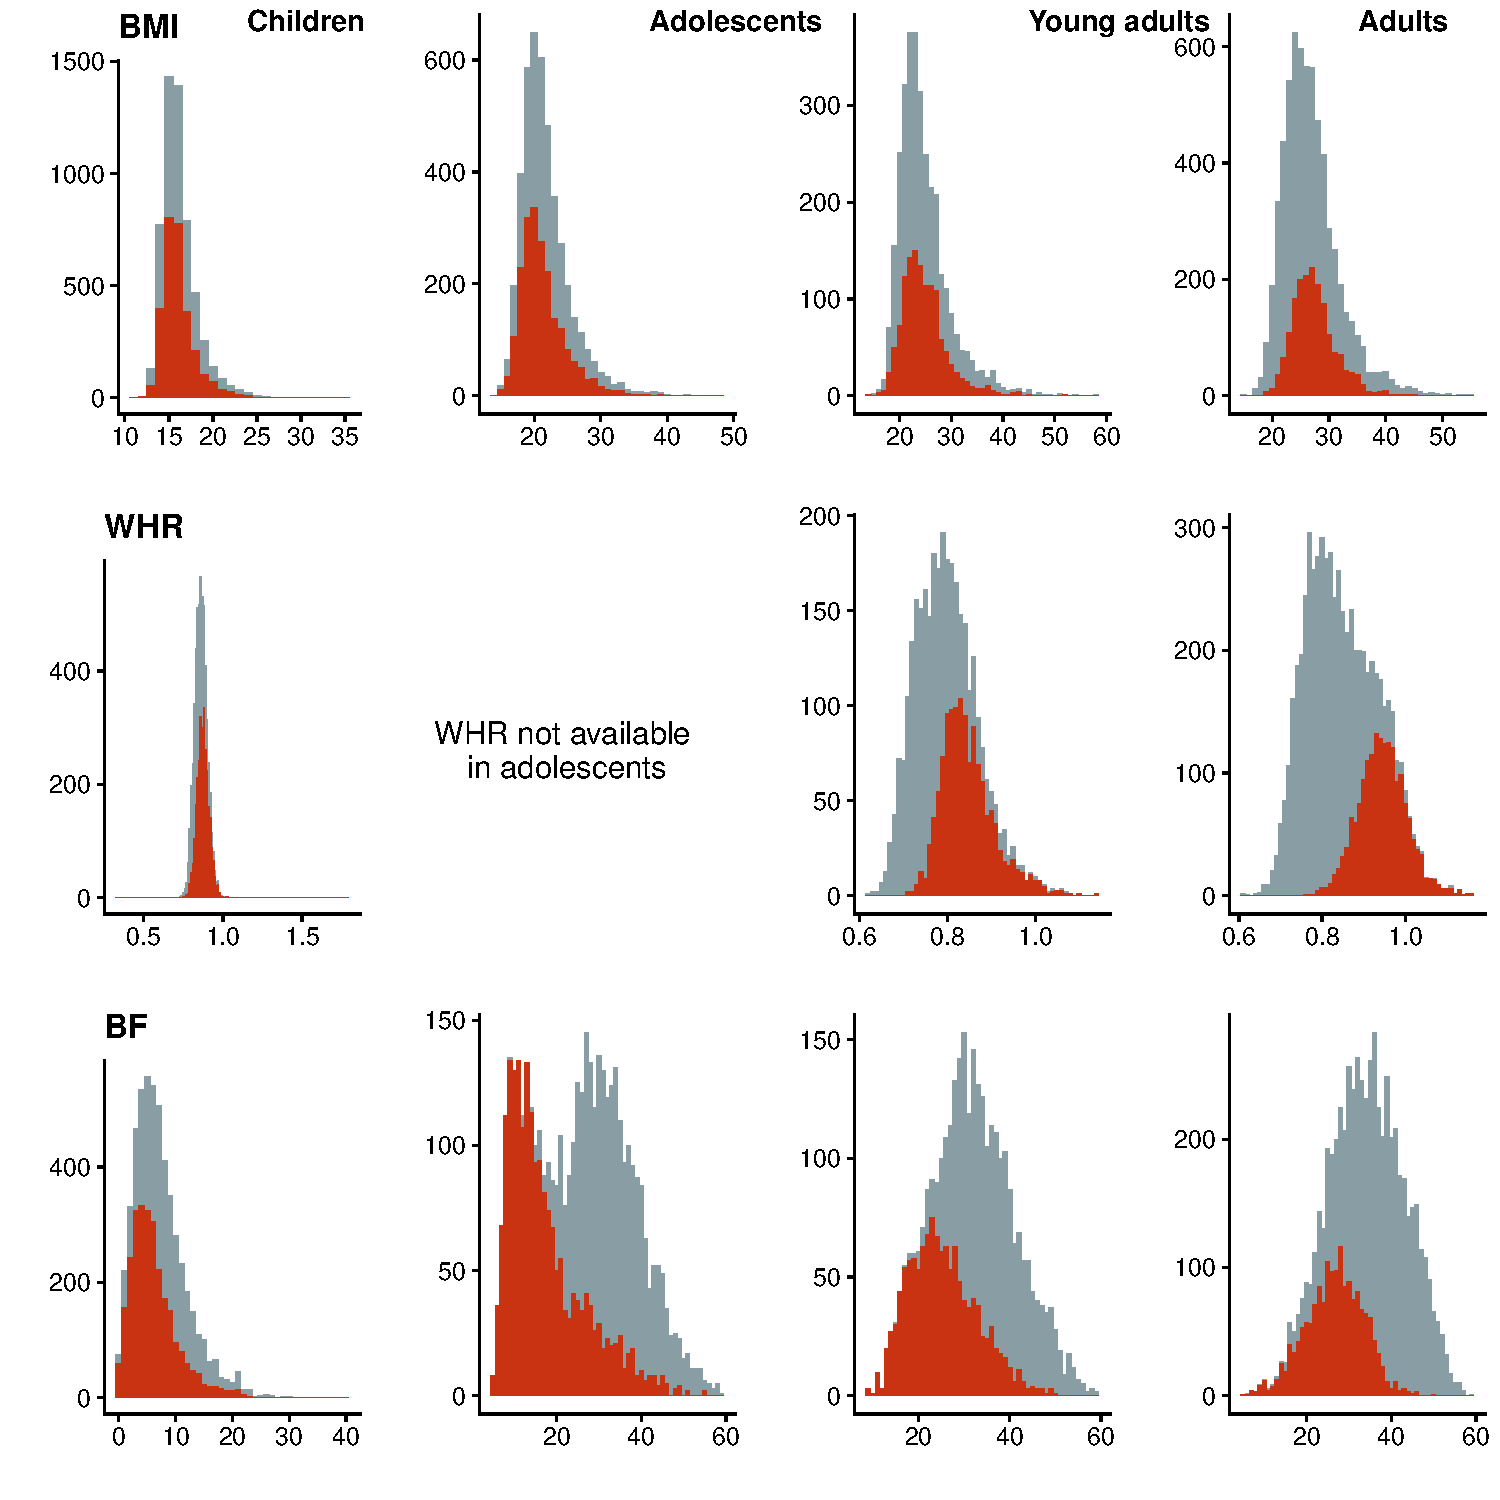
\includegraphics[width=1\linewidth]{data/observational/figures/plot_histogram_adiposity_measures} 

}

\caption[Distribution of adiposity measures across all age groups]{\textbf{Distribution of adiposity measures across all age groups}. Plots give the distribution of all adiposity measures across age groups by sex. Body fat percentage (BF) in children is derived from equation \eqref{eq:BF}. BMI = body mass index; WHR = waist hip ratio. Data is presented for all individuals given in Table \ref{tab:observational-table-ALSPAC-adiposity}. The interquartile range and median are also shown. Raincloud plots produced using the \texttt{RainCloudPlots} \texttt{R} package\textsuperscript{\protect\hyperlink{ref-Allen2019}{660}}.}\label{fig:appendix-observational-figure-adiposity-distribution}
\end{figure}
\hypertarget{appendix-observational-figures}{%
\subsubsection{Linear regression results}\label{appendix-observational-figures}}

The following two forest plots show the results from linear regression analysis for all exposures and age groups for model 2 (age, sex, maternal or own education, smoking status, alcohol consumption, diet (calories consumed per day)). The first plot shows all directly measured metabolites; the second plot shows derived metabolite measures such as ratios. Four Circos plots are presented after this; each Circos plot shows the results from linear regression analysis for all exposures within an age group for model 2.

\par





\blandscape
\begin{figure}

{\centering 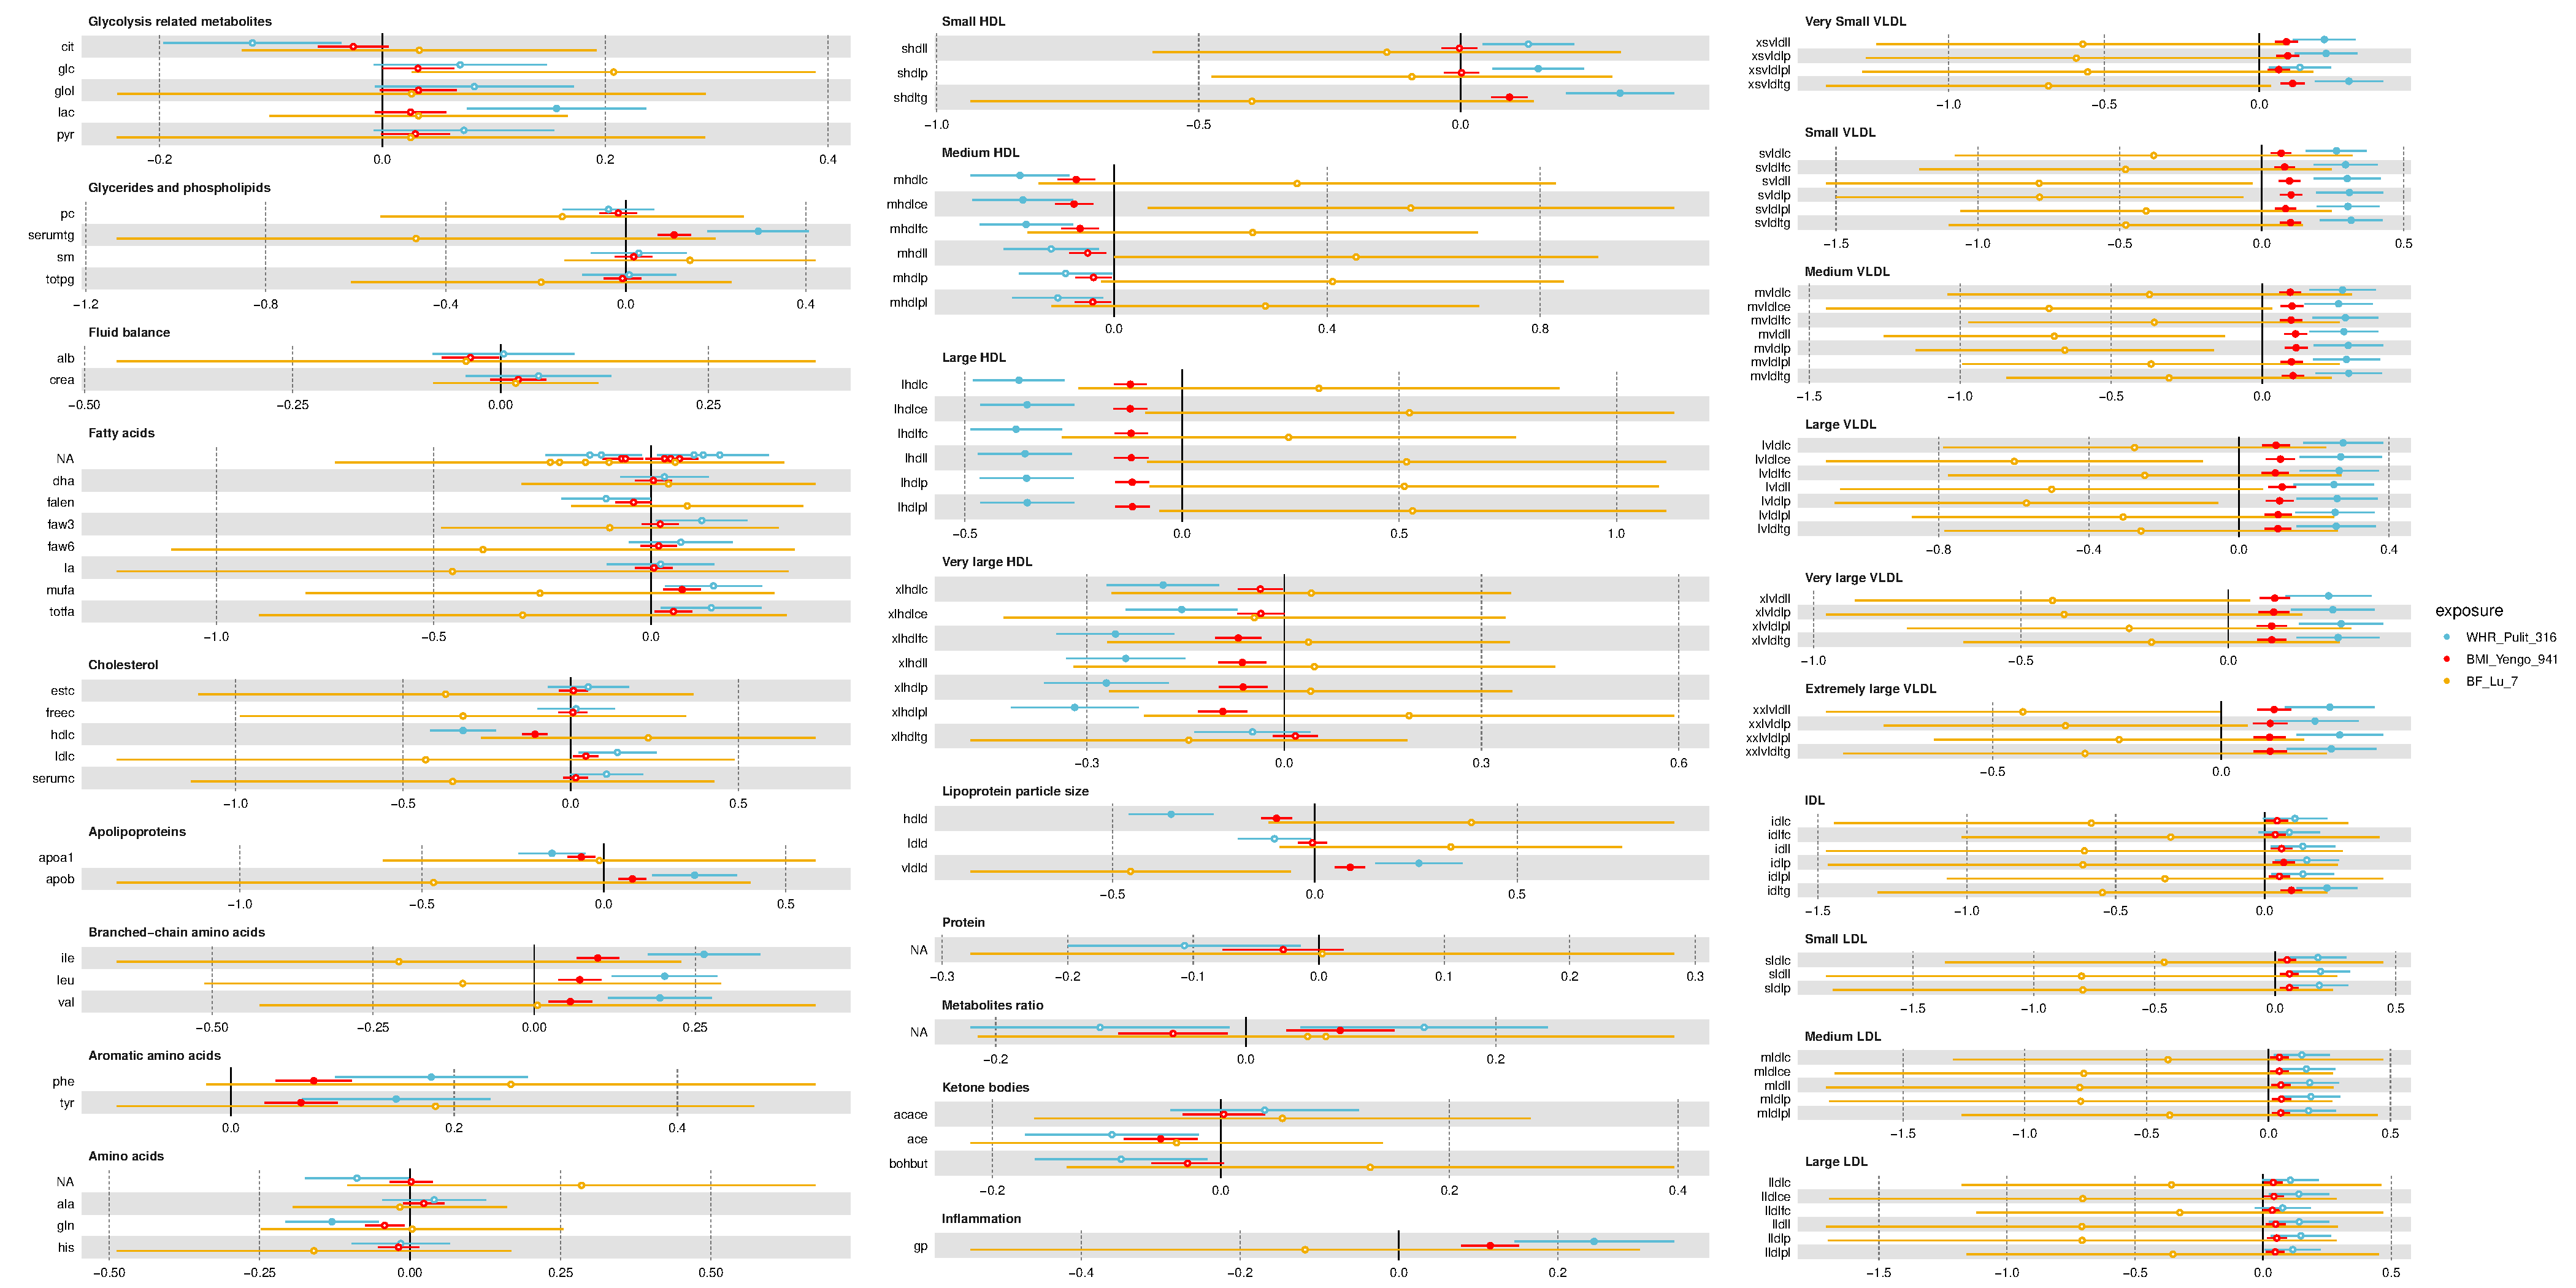
\includegraphics[width=1\linewidth]{data/observational/figures/forestplot_main} 

}

\caption[Linear regression analysis: association between adiposity measures and directly measured metabolites]{\textbf{Linear regression analysis: association between adiposity measures and directly measured metabolites}. Forest plot shows effect estimates and 95\% confidence intervals from model 2 (age, sex, maternal or own education, smoking status, alcohol consumption, diet (calories consumed per day)) for all exposures and age groups. Units represent the unit change in each metabolite per standard deviation change in the exposure. Available on \href{https://github.com/mattlee821/000_thesis/blob/master/index/data/observational/figures/forestplot_main.pdf}{GitHub}. An alternative forest plot in long form is also available on \href{https://github.com/mattlee821/000_thesis/blob/master/index/data/observational/figures/forestplot_all_metabolites_long.pdf}{GitHub}.}\label{fig:appendix-observational-figure-forestplot-main}
\end{figure}
\elandscape





\blandscape
\begin{figure}

{\centering 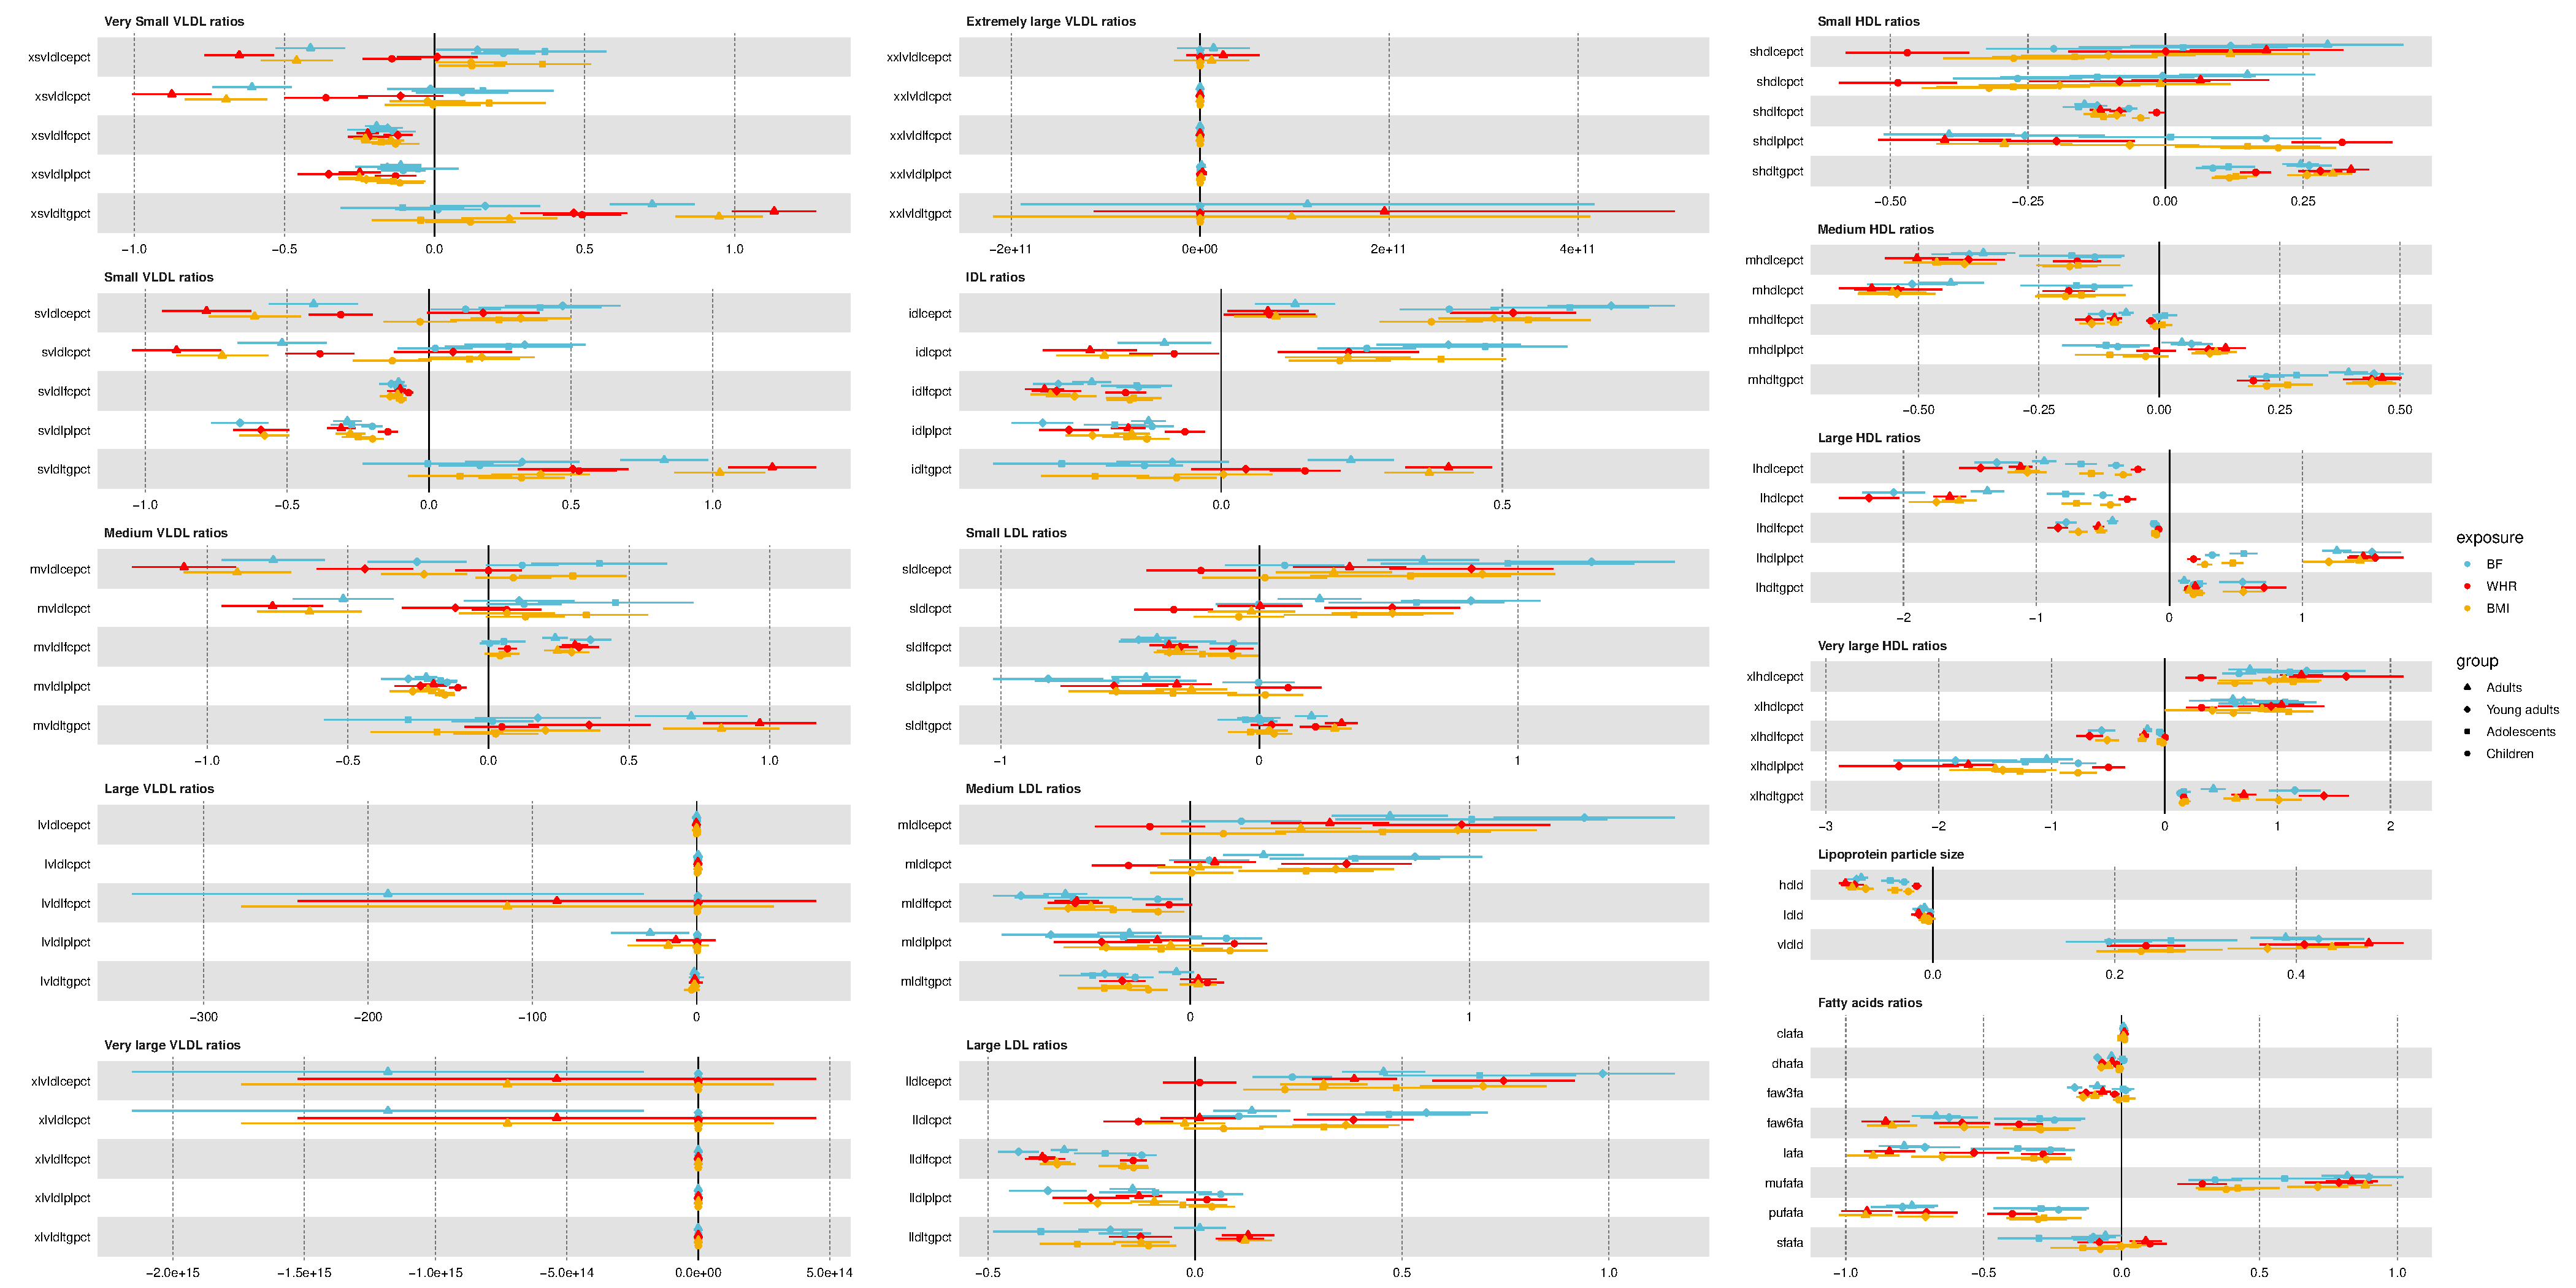
\includegraphics[width=1\linewidth]{data/observational/figures/forestplot_supplement} 

}

\caption[Linear regression analysis: association between adiposity measures and derived metabolites]{\textbf{Linear regression analysis: association between adiposity measures and derived metabolites}. Forest plot shows effect estimates and 95\% confidence intervals from model 2 (age, sex, maternal or own education, smoking status, alcohol consumption, diet (calories consumed per day)) for all exposures and age groups. Units represent the unit change in each metabolite per standard deviation change in the exposure. Available on \href{https://github.com/mattlee821/000_thesis/blob/master/index/data/observational/figures/forestplot_supplement.pdf}{GitHub}. An alternative forest plot in long form is also available on \href{https://github.com/mattlee821/000_thesis/blob/master/index/data/observational/figures/forestplot_all_metabolites_long.pdf}{GitHub}.}\label{fig:appendix-observational-figure-forestplot-derived}
\end{figure}
\elandscape




\begin{figure}

{\centering 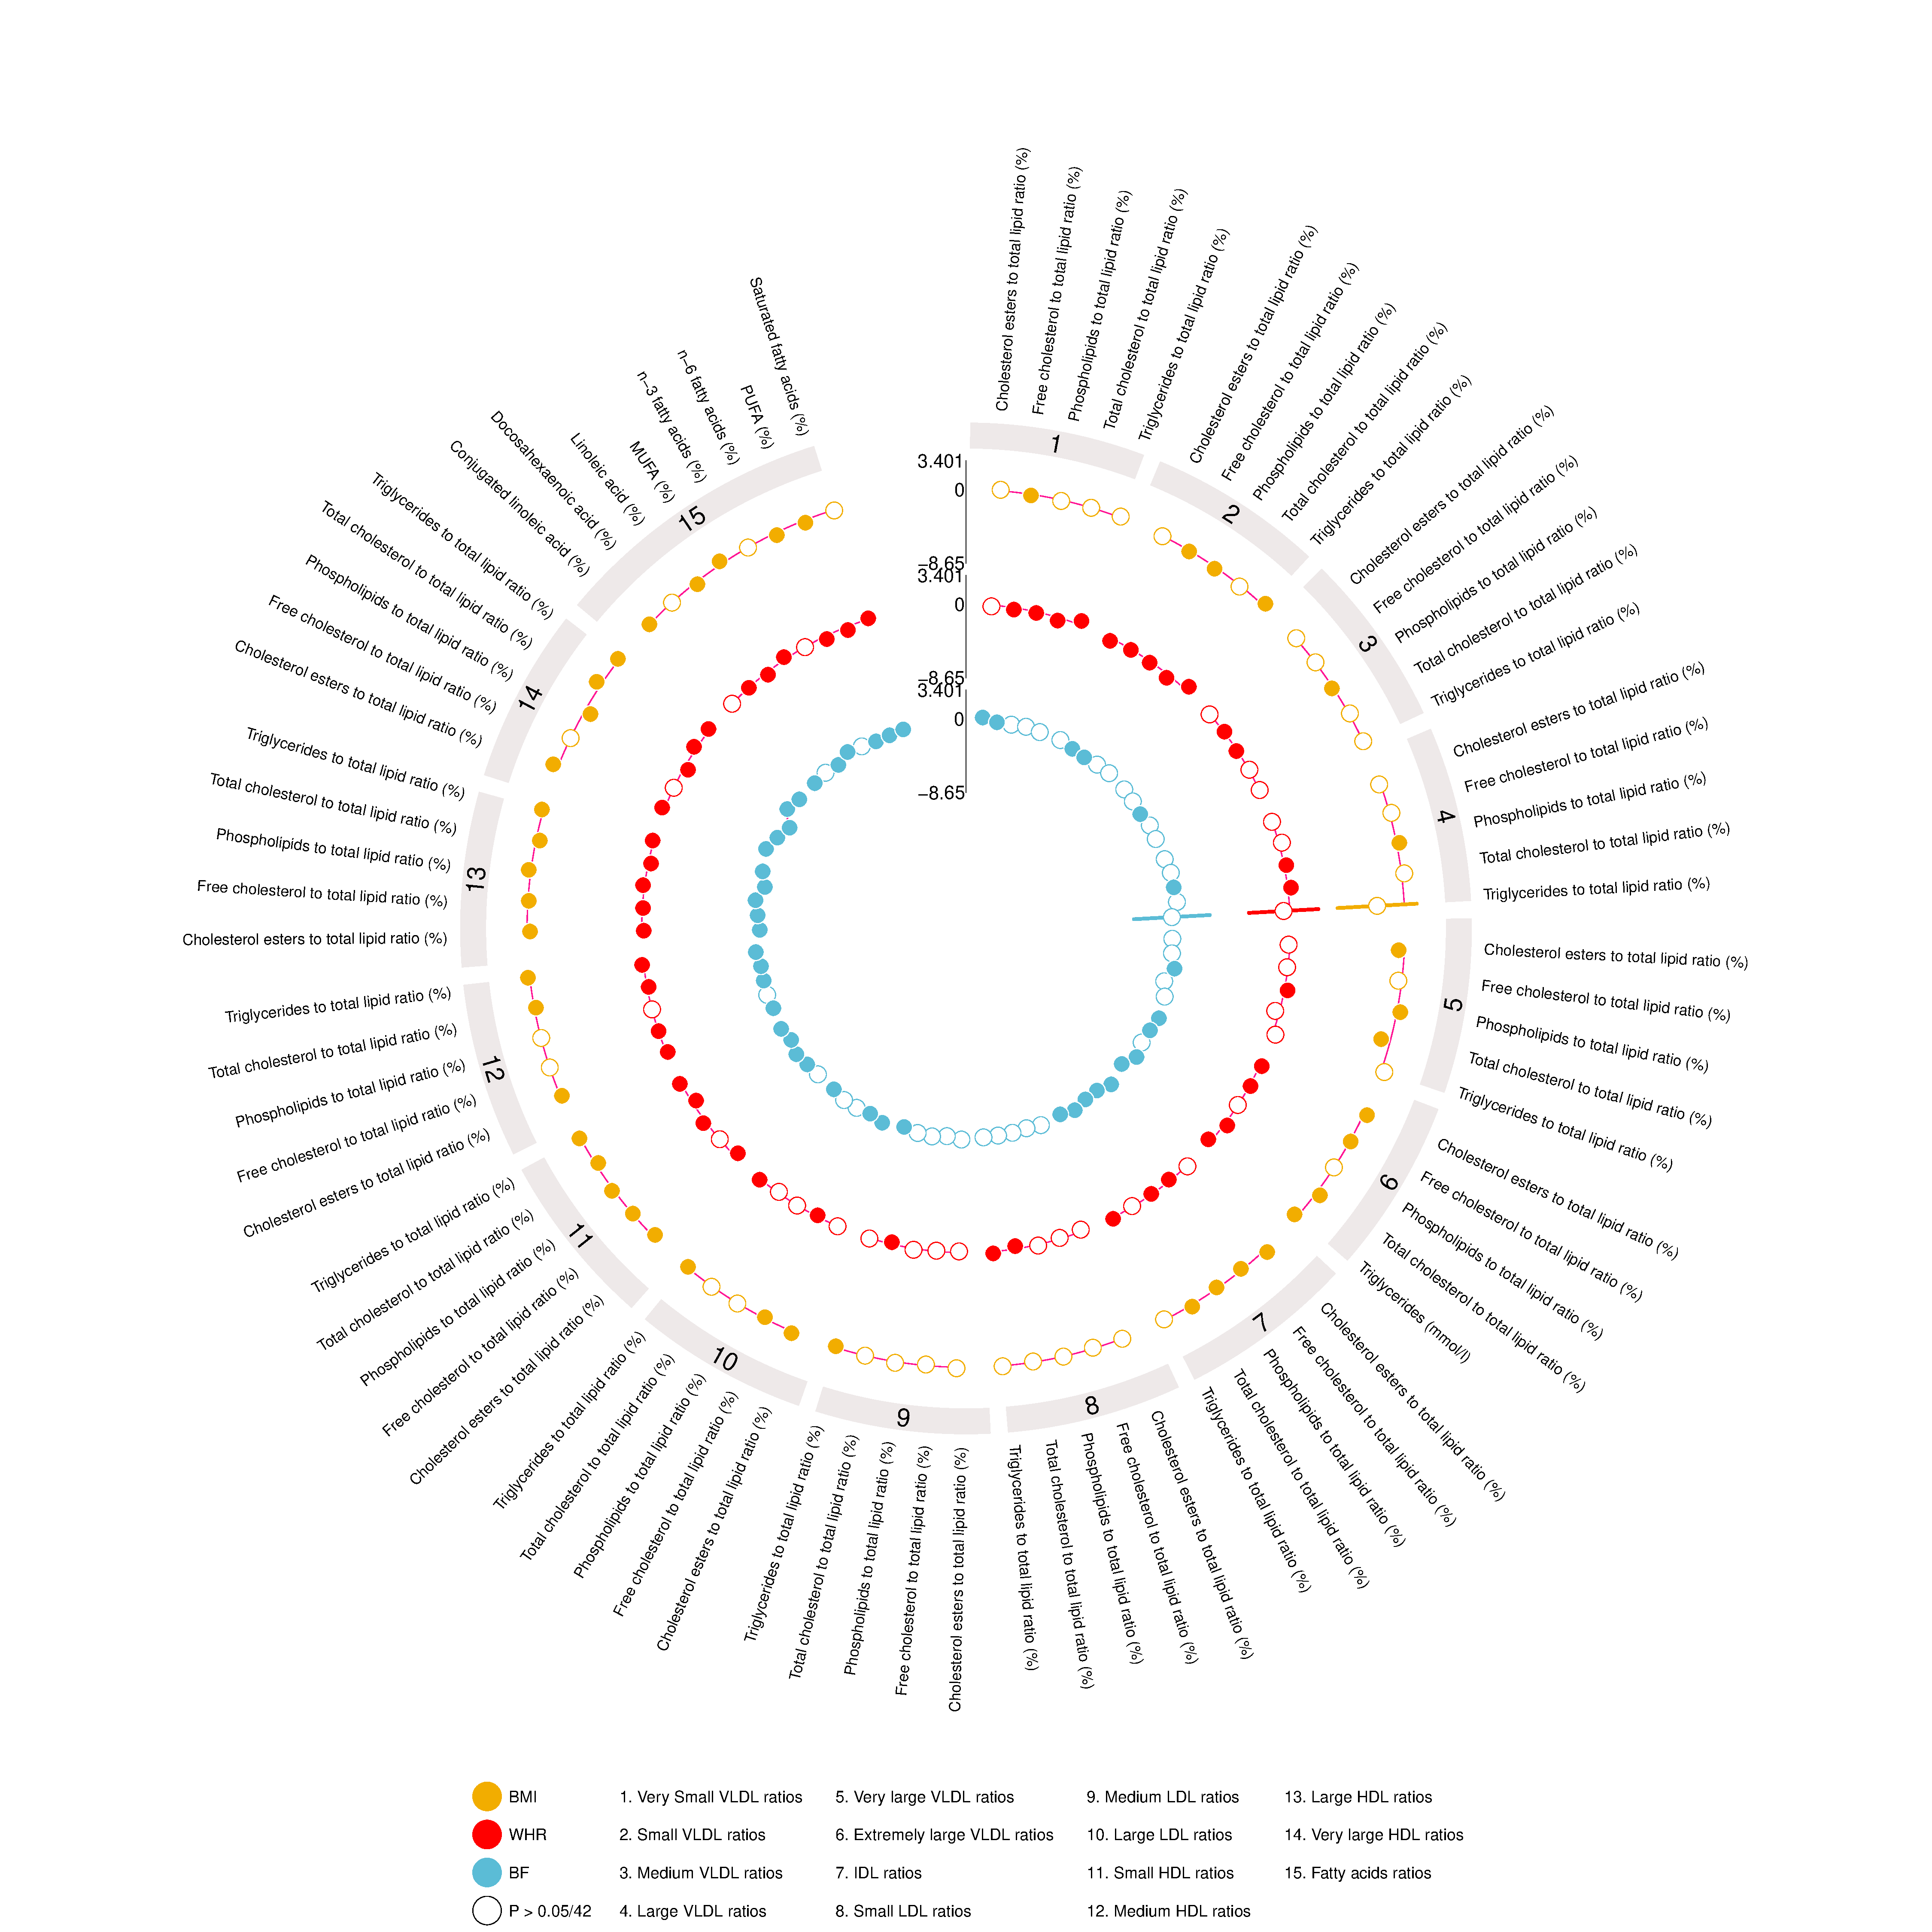
\includegraphics[width=1\linewidth]{data/observational/figures/circosplot_derived_metabolites_children} 

}

\caption[Linear regression analysis: association between adiposity measures and derived metabolites in children]{\textbf{Linear regression analysis: association between adiposity measures and derived metabolites in children}. Circos plot shows effect estimates and 95\% confidence intervals from model 2 for all exposures in children. Effect estimates are absolute change in metabolite per standard deviation increase in exposure. The outer track is body mass index (BMI), the middle track is waist hip ratio (WHR), the inner track is body fat percentage (BF). Solid points indicate a multiple testing threshold has been met; multiple testing threshold (0.05/54) set as the number of independent metabolite features as calculated by \texttt{metaboprep}. Available on \href{https://github.com/mattlee821/000_thesis/blob/master/index/data/observational/figures/circosplot_derived_metabolites_children.pdf}{GitHub}.}\label{fig:appendix-observational-figure-circos-children}
\end{figure}



\begin{figure}

{\centering 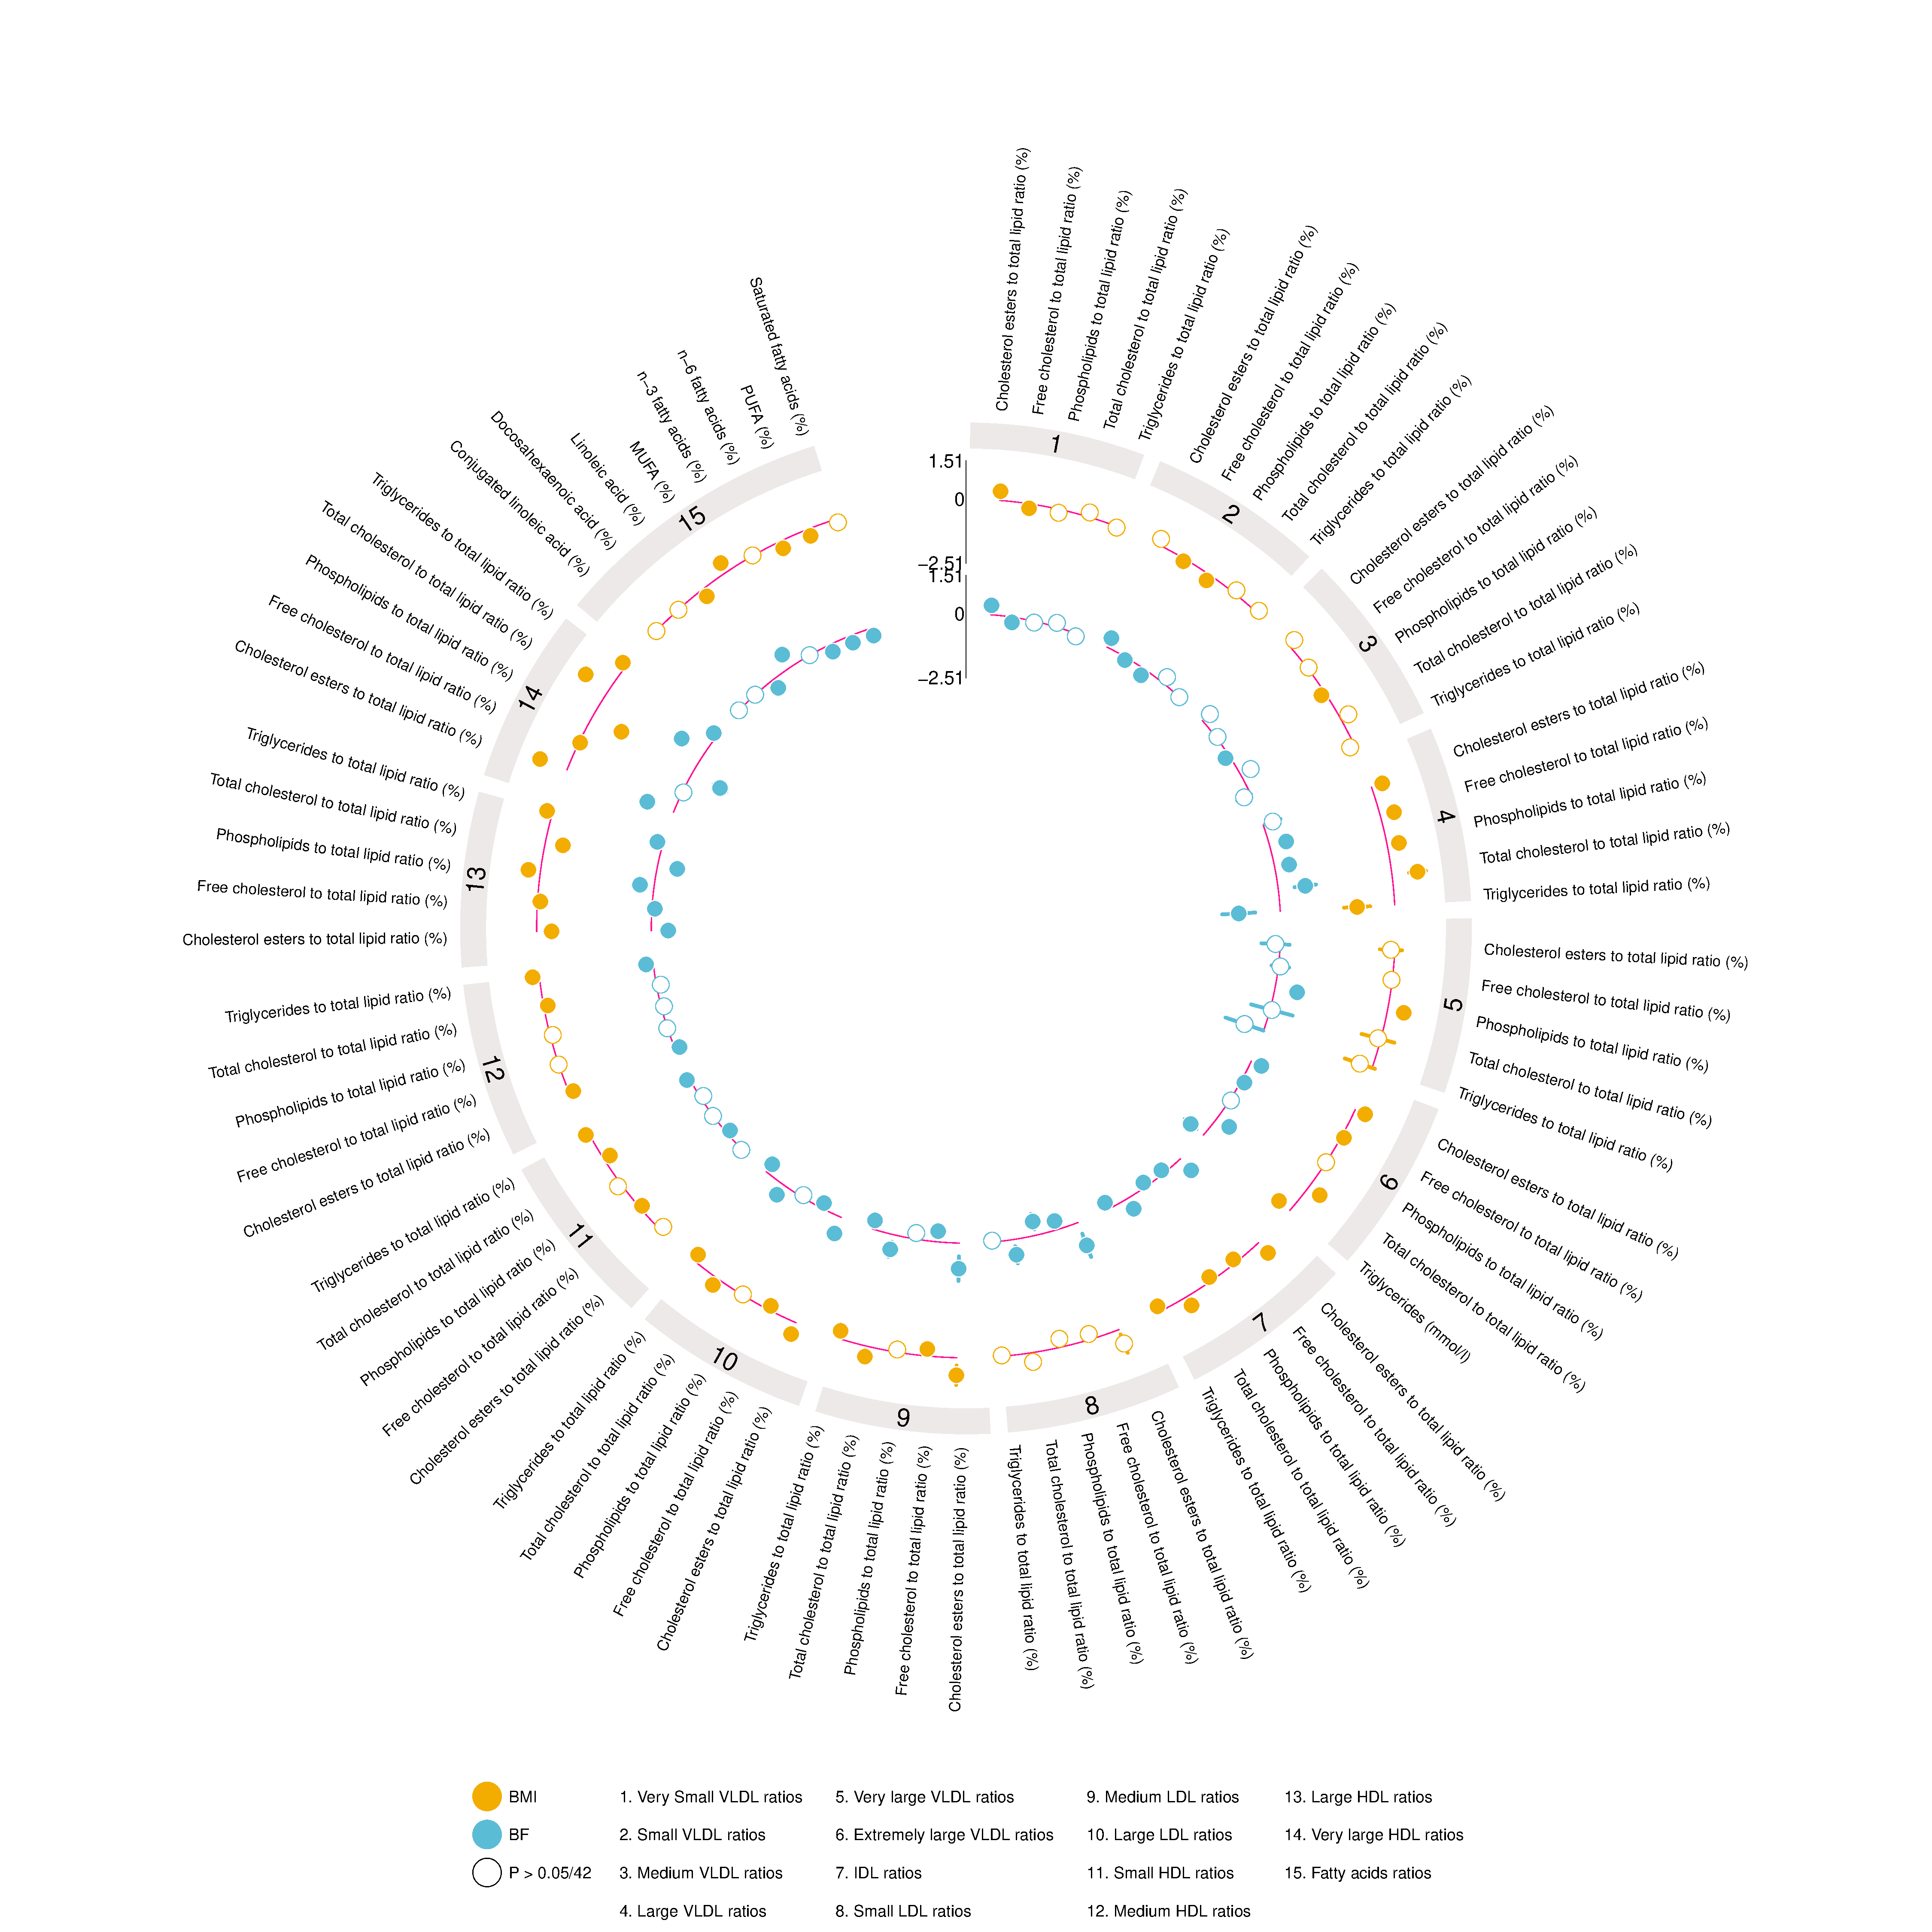
\includegraphics[width=1\linewidth]{data/observational/figures/circosplot_derived_metabolites_adolescents} 

}

\caption[Linear regression analysis: association between adiposity measures and derived metabolites in adolescents]{\textbf{Linear regression analysis: association between adiposity measures and derived metabolites in adolescents}. Circos plot shows effect estimates and 95\% confidence intervals from model 2 for all exposures in adolescents. Effect estimates are absolute change in metabolite per standard deviation increase in exposure. The outer track is body mass index (BMI), the inner track is body fat percentage (BF). Solid points indicate a multiple testing threshold has been met; multiple testing threshold (0.05/48) set as the number of independent metabolite features as calculated by \texttt{metaboprep}. Available on \href{https://github.com/mattlee821/000_thesis/blob/master/index/data/observational/figures/circosplot_derived_metabolites_adolescents.pdf}{GitHub}.}\label{fig:appendix-observational-figure-circos-adolescents}
\end{figure}



\begin{figure}

{\centering \includegraphics[width=1\linewidth]{data/observational/figures/circosplot_derived_metabolites_young_adults} 

}

\caption[Linear regression analysis: association between adiposity measures and derived metabolites in young adults]{\textbf{Linear regression analysis: association between adiposity measures and derived metabolites in young adults}. Circos plot shows effect estimates and 95\% confidence intervals from model 2 for all exposures in young adults. Effect estimates are absolute change in metabolite per standard deviation increase in exposure. The outer track is body mass index (BMI), the middle track is waist hip ratio (WHR), the inner track is body fat percentage (BF). Solid points indicate a multiple testing threshold has been met; multiple testing threshold (0.05/46) set as the number of independent metabolite features as calculated by \texttt{metaboprep}. Available on \href{https://github.com/mattlee821/000_thesis/blob/master/index/data/observational/figures/circosplot_derived_metabolites_young_adults.pdf}{GitHub}.}\label{fig:appendix-observational-figure-circos-young-adults}
\end{figure}



\begin{figure}

{\centering \includegraphics[width=1\linewidth]{data/observational/figures/circosplot_derived_metabolites_adults} 

}

\caption[Linear regression analysis: association between adiposity measures and derived metabolites in adults]{\textbf{Linear regression analysis: association between adiposity measures and derived metabolites in adults}. Circos plot shows effect estimates and 95\% confidence intervals from model 2 for all exposures in adults. Effect estimates are absolute change in metabolite per standard deviation increase in exposure. The outer track is body mass index (BMI), the middle track is waist hip ratio (WHR), the inner track is body fat percentage (BF). Solid points indicate a multiple testing threshold has been met; multiple testing threshold (0.05/53) set as the number of independent metabolite features as calculated by \texttt{metaboprep}. Available on \href{https://github.com/mattlee821/000_thesis/blob/master/index/data/observational/figures/circosplot_derived_metabolites_adults.pdf}{GitHub}.}\label{fig:appendix-observational-figure-circos-adults}
\end{figure}
\newpage

\hypertarget{appendix-MR}{%
\section{Chapter 5: Associations between multiple measures of adiposity and metabolites: Mendelian randomization analysis}\label{appendix-MR}}

In Chapter \ref{MR}, the association between adiposity measures and NMR derived metabolites and ratios was investigated using MR. Summary statistics from multiple genome-wide association studies (GWAS) were used to obtain genetic variants (single nucleotide polymorphisms; SNPs). The following sections on exposures detail the GWAS used in additional analyses in Chapter \ref{MR} which aimed to test the validity of instruments used in the main analysis. The outcomes section gives a table of metabolites used in these analyses. The results sections present figures for the sensitivity and additional analyses described and summarised in the main text of Chapter \ref{MR}.

\par

\hypertarget{methods-3}{%
\subsection{Methods}\label{methods-3}}

\hypertarget{appendix-MR-exposures}{%
\subsubsection{Exposure instruments}\label{appendix-MR-exposures}}

In the main analysis, BMI, WHR, and BF were instrumented using SNPs from Yengo et al.~(2018)\textsuperscript{\protect\hyperlink{ref-Yengo2018}{53}}, Pulit et al.~(2019)\textsuperscript{\protect\hyperlink{ref-Pulit2019}{54}}, and Lu et al.~(206)\textsuperscript{\protect\hyperlink{ref-Lu2016}{51}}, respectively. Additional instrument lists were obtained for each of the adiposity measures. A list of all instruments used is available on \href{https://github.com/mattlee821/000_thesis/blob/master/index/data/MR/tables/exposure_SNPs.txt}{GitHub}. The following details the GWAS from which summary statistics for these additional SNP lists were obtained.

\par

\hypertarget{body-mass-index-2}{%
\paragraph{Body mass index}\label{body-mass-index-2}}

Two additional instrument lists were used for BMI. The first came from the same study as used in the main analysis (Yengo et al.~(2019)) but did not use the conditional and joint analysis (COJO) GWAS summary statistics. COJO analyses attempt to identify secondary signals (SNPs) at each genome-wide association study (GWAS) identified loci after controlling for linkage disequilibrium (LD). That is, the presence of a secondary signal is conditional on the presence of the first\textsuperscript{\protect\hyperlink{ref-Yang2012}{661}}. As such, COJO analyses may increase the number of available genetic instruments for MR analysis without introducing additional biases as a result of LD, such as falsely narrow confidence intervals (CIs). Few studies have investigated the use of COJO-GWAS summary statistics in MR analyses. The study by Yew et al., (2020)\textsuperscript{\protect\hyperlink{ref-Yew2020}{662}}, which used the Yengo et al.~(2019) COJO-GWAS for BMI, found little evidence for a difference in resulting effect estimates of the association between BMI and atopic dermatitis when using the 941-SNP genetic instrument compared to instruments with different LD (thresholds included r\textsuperscript{2} 0.001, 0.001, 0.1, 0.2, and 0.5) pruning thresholds. They did not however compare results to the Yengo et al., (2019) non-COJO-GWAS for BMI. The GWAS for the non-COJO and COJO genetic instruments were the same, and are presented in the main text. Briefly, data were available from 515,509--795,624 individuals of European ancestries from two sources, the Genetic Investigation of Anthropometric Traits (GIANT) consortium\textsuperscript{\protect\hyperlink{ref-Locke2015}{48}} and UK Biobank. In both sources, BMI was calculated as \(\displaystyle \frac{weight\ (kg)}{height\ (m^2)}\). Yengo et al., (2018)\textsuperscript{\protect\hyperlink{ref-Yengo2018}{53}} performed a fixed effects inverse variance weighted meta-analysis of BMI using GWAS results generated from UK Biobank (N = 456,426) and results from the GIANT consortium, Locke et al., (2015)\textsuperscript{\protect\hyperlink{ref-Locke2015}{48}} (N = 322,154) using METAL\textsuperscript{\protect\hyperlink{ref-Willer2010}{551}}. A total of 656 primary associations (i.e., non-COJO SNPs) reaching a genome-wide significance threshold of p-value \textless{} 5 x 10\textsuperscript{-8} were identified and used for the additional analysis here.

\par

The second instrument list came from Locke et al.~(2015), in which 322,154 individuals of European ancestries were included in a fixed effects inverse variance weighted meta-analysis. This GWAS was the GIANT component of the Yengo et al., meta-analysis, and is described in detail in the main text of Chapter \ref{MR}. Briefly, a total of 82 GWAS and 43 studies using the Metabochip array were included in the meta-analysis by Locke et al.~Individual GWAS were adjusted for age, age-squared, and study specific covariates with residuals inverse rank normally transformed. Imputation was performed using the HapMap phase II Utah residents of Northern and Western European ancestries (CEU) reference panel. Each study used a linear regression model assuming an additive genetic model with quality control following procedures outlined previously\textsuperscript{\protect\hyperlink{ref-Winkler2014}{598}}. A fixed effect inverse variance weighted meta-analysis was performed using METAL for the 82 GWAS and 43 studies using the Metabochip array separately. The final meta-analysis combined the GWAS meta-analysis and Metabochip meta-analysis results using a fixed effects inverse variance weighted model. A total of 77 loci reaching genome-wide significance (p-value \textless{} 5 x 10\textsuperscript{-8}) and separated by at least 500 kilobases were identified and used for the addional analysis here.

\par

\hypertarget{waist-hip-ratio-2}{%
\paragraph{Waist hip ratio}\label{waist-hip-ratio-2}}

In the main MR analysis, summary statistics for waist hip ratio (WHR) from Pulit et al.~(2019) were used. Pulit et al., performed a fixed effects inverse variance weighted meta-analysis from two sources, UK Biobank and the GIANT consortium. For the UK Biobank GWAS, the second release (June 2017) of UK Biobank data, which did not have corrected imputation at non-human reference consortium (HRC) sites, was used. Briefly, data were available from 485,486---697,702 individuals of European ancestries from two sources, UK Biobank and the GIANT consortium\textsuperscript{\protect\hyperlink{ref-Shungin2015}{49}}. In both sources, WHR was calculated as \(\displaystyle \frac{waist\ circumference\ (cm)} {hip\ circumference\ (cm)}\). Pulit et al., (2019)\textsuperscript{\protect\hyperlink{ref-Pulit2019}{54}} performed a fixed effects inverse variance weighted meta-analysis of WHR using GWAS results generated from UK Biobank (N up to 485,486 (men up to 263,148; women up to 222,338)) and results from the GIANT consortium (N up to 212,248 (men up to 94,434; women up to 118,004))\textsuperscript{\protect\hyperlink{ref-Shungin2015}{49}} using METAL. The GIANT component of this meta-analysis was used in the additional analysis here.

\par

In GIANT, Shungin et al., (2015)\textsuperscript{\protect\hyperlink{ref-Shungin2015}{49}} performed a fixed effects inverse variance weighted meta-analysis of up to 212,248 individuals of European ancestries. Individual studies recruited participants and undertook sample and SNP quality control. These studies used genome-wide or Metabochip arrays for sequencing. In studies using genome-wide arrays, imputation was performed with CEU haplotypes from HapMap. Metabochip arrays target specific genetic variants and imputation was not performed. For both study types, an additive genetic model was assumed, with each study running a linear regression GWAS. Sex-specific summary statistics were corrected for population structure using the genomic control inflation factor. Prior to meta-analysis of the genome-wide array GWAS and Metabochip array GWAS, SNPs were removed if they had a minor allele count \(\leq\) 3, were not in Hardy-Weinberg equilibrium (p-value \textless{} 10\textsuperscript{-6}), had a call rate \textless{} 95\% or an imputation quality score \textless{} 0.3 for MACH, \textless{} 0.4 for IMPUTE, and \textless{} 0.8 for PLINK. In step 1, a meta-analysis of each array was performed using a fixed effects inverse variance weighted model and corrected for genomic control to account for structure between cohorts. In step 2, summary statistics from the meta-analysis of genome-wide array and Metabochip array GWAS were meta-analysed using a fixed effects inverse variance weighted model using METAL. In this second step genomic correction was not performed. In total, 210,088 individuals of European ancestries were included. A total of 26 loci reaching genome-wide significance (p-value \textless{} 5 x 10\textsuperscript{-8}) and separated by at least 500 kilobases were identified and used in additional analysis here.

\par

\hypertarget{body-fat-percentage-2}{%
\paragraph{Body fat percentage}\label{body-fat-percentage-2}}

For BF, two additional instruments were used. The first used summary statistics from the study by Lu et al.~(2016)\textsuperscript{\protect\hyperlink{ref-Lu2016}{51}}, used in the main analysis, after removal of two SNPs which had been previously associated with `favourable adiposity'\textsuperscript{\protect\hyperlink{ref-Yaghootkar2014}{47},\protect\hyperlink{ref-Yaghootkar2016}{557}}. The second came from summary statistics from Hubel et al.~(2019)\textsuperscript{\protect\hyperlink{ref-Hubel2019}{55}} who analysed data from up to 155,961 (female = 70,700; male = 85,261) individuals of European ancestries from UK Biobank. Body composition was assessed using bioelectrical impedance (Tanita BC-418 MA; Tanita Corporation, Arlington Heights, IL); fat mass and fat free mass was calculated from raw impedance data adjusting for age, sex, height and athleticism (variable not described). BF was calculated as \(\displaystyle \frac{fat\ mass\ (kg)} {weight\ (kg)}\ *\ 100\). Hubel et al., performed a fixed effects inverse variance weighted meta-analysis of two sex-specific GWAS using METAL. The sex-specific GWAS were performed using a linear regression model assuming an additive genetic model using BGENIE (V1.2). BF residuals were adjusted for age, socioeconomic status (measured by Townsend deprivation index), assessment centre, genotyping batch, smoking status, alcohol consumption, menopause and the first 6 PCs. Genotypes were imputed to the Human Reference Consortium. A total of 76 loci reaching a genome-wide significance threshold of p-value \textless{} 5 x 10\textsuperscript{-8} and separated by at least 3,000 kilobases were identified and used in additional analysis here.

\par

\newpage

\hypertarget{metabolites-1}{%
\subsubsection{Metabolites}\label{metabolites-1}}

\begingroup\fontsize{8}{10}\selectfont
\begin{ThreePartTable}
\begin{TableNotes}[para]
\item Table gives the metabolite abbreviation, label with originally measured units, class and subclass the metabolites were grouped in, whether the metabolite is a derived measure such as a ratio, and the study in which they were available. HDL = high density lipoprotein; LDL = low density lipoprotein; IDL = intermediate density lipoprotein; VLDL = very large low density lipoprotein.
\end{TableNotes}
\begin{longtabu} to \linewidth {>{\raggedright\arraybackslash}p{5em}>{\raggedright\arraybackslash}p{20em}>{\raggedright\arraybackslash}p{10em}>{\raggedright\arraybackslash}p{10em}>{\raggedright\arraybackslash}p{3em}>{\raggedright\arraybackslash}p{3em}}
\caption{\label{tab:appendix-MR-table-metabolites}Metabolites used in Mendelian randomization analyses}\\
\toprule
Metabolite & Label & Class & Subclass & Derived & Study\\
\midrule
\endfirsthead
\caption[]{\label{tab:appendix-MR-table-metabolites}Metabolites used in Mendelian randomization analyses \textit{(continued)}}\\
\toprule
Metabolite & Label & Class & Subclass & Derived & Study\\
\midrule
\endhead

\endfoot
\bottomrule
\insertTableNotes
\endlastfoot
\cellcolor{gray!6}{ala} & \cellcolor{gray!6}{Alanine (mmol/l)} & \cellcolor{gray!6}{Amino acids} & \cellcolor{gray!6}{Amino acids} & \cellcolor{gray!6}{no} & \cellcolor{gray!6}{Both}\\
gln & Glutamine (mmol/l) & Amino acids & Amino acids & no & Both\\
\cellcolor{gray!6}{gly} & \cellcolor{gray!6}{Glycine  (mmol/l)} & \cellcolor{gray!6}{Amino acids} & \cellcolor{gray!6}{Amino acids} & \cellcolor{gray!6}{no} & \cellcolor{gray!6}{INTERVAL}\\
his & Histidine (mmol/l) & Amino acids & Amino acids & no & Both\\
\cellcolor{gray!6}{} & \cellcolor{gray!6}{Urea} & \cellcolor{gray!6}{Amino acids} & \cellcolor{gray!6}{Amino acids} & \cellcolor{gray!6}{} & \cellcolor{gray!6}{Kettunen}\\
\addlinespace
phe & Phenylalanine (mmol/l) & Amino acids & Aromatic amino acids & no & Both\\
\cellcolor{gray!6}{tyr} & \cellcolor{gray!6}{Tyrosine (mmol/l)} & \cellcolor{gray!6}{Amino acids} & \cellcolor{gray!6}{Aromatic amino acids} & \cellcolor{gray!6}{no} & \cellcolor{gray!6}{Both}\\
ile & Isoleucine (mmol/l) & Amino acids & Branched-chain amino acids & no & Both\\
\cellcolor{gray!6}{leu} & \cellcolor{gray!6}{Leucine (mmol/l)} & \cellcolor{gray!6}{Amino acids} & \cellcolor{gray!6}{Branched-chain amino acids} & \cellcolor{gray!6}{no} & \cellcolor{gray!6}{Both}\\
val & Valine (mmol/l) & Amino acids & Branched-chain amino acids & no & Both\\
\addlinespace
\cellcolor{gray!6}{apoa1} & \cellcolor{gray!6}{Apolipoprotein A-I (g/l)} & \cellcolor{gray!6}{Apolipoproteins} & \cellcolor{gray!6}{Apolipoproteins} & \cellcolor{gray!6}{no} & \cellcolor{gray!6}{Both}\\
apob & Apolipoprotein B (g/l) & Apolipoproteins & Apolipoproteins & no & Both\\
\cellcolor{gray!6}{apobapoa1} & \cellcolor{gray!6}{Ratio of apolipoprotein B to apolipoprotein A-I} & \cellcolor{gray!6}{Apolipoproteins} & \cellcolor{gray!6}{Apolipoproteins} & \cellcolor{gray!6}{no} & \cellcolor{gray!6}{INTERVAL}\\
estc & Esterified cholesterol (mmol/l) & Cholesterol & Cholesterol & no & Both\\
\cellcolor{gray!6}{freec} & \cellcolor{gray!6}{Free cholesterol (mmol/l)} & \cellcolor{gray!6}{Cholesterol} & \cellcolor{gray!6}{Cholesterol} & \cellcolor{gray!6}{no} & \cellcolor{gray!6}{Both}\\
\addlinespace
remnantc & Remnant cholesterol (non-HDL, non-LDL -cholesterol) (mmol/l) & Cholesterol & Cholesterol & no & INTERVAL\\
\cellcolor{gray!6}{serumc} & \cellcolor{gray!6}{Serum total cholesterol (mmol/l)} & \cellcolor{gray!6}{Cholesterol} & \cellcolor{gray!6}{Cholesterol} & \cellcolor{gray!6}{no} & \cellcolor{gray!6}{Both}\\
hdlc & Total cholesterol in HDL (mmol/l) & Cholesterol & Cholesterol & no & Both\\
\cellcolor{gray!6}{hdl2c} & \cellcolor{gray!6}{Total cholesterol in HDL2 (mmol/l)} & \cellcolor{gray!6}{Cholesterol} & \cellcolor{gray!6}{Cholesterol} & \cellcolor{gray!6}{no} & \cellcolor{gray!6}{INTERVAL}\\
hdl3c & Total cholesterol in HDL3 (mmol/l) & Cholesterol & Cholesterol & no & INTERVAL\\
\addlinespace
\cellcolor{gray!6}{ldlc} & \cellcolor{gray!6}{Total cholesterol in LDL (mmol/l)} & \cellcolor{gray!6}{Cholesterol} & \cellcolor{gray!6}{Cholesterol} & \cellcolor{gray!6}{no} & \cellcolor{gray!6}{Both}\\
vldlc & Total cholesterol in VLDL (mmol/l) & Cholesterol & Cholesterol & no & INTERVAL\\
\cellcolor{gray!6}{la} & \cellcolor{gray!6}{18:2, linoleic acid (mmol/l)} & \cellcolor{gray!6}{Fatty acids} & \cellcolor{gray!6}{Fatty acids} & \cellcolor{gray!6}{no} & \cellcolor{gray!6}{Both}\\
dha & 22:6, docosahexaenoic acid (mmol/l) & Fatty acids & Fatty acids & no & Both\\
\cellcolor{gray!6}{} & \cellcolor{gray!6}{Average number of double bonds in a fatty acid chain} & \cellcolor{gray!6}{Fatty acids} & \cellcolor{gray!6}{Fatty acids} & \cellcolor{gray!6}{} & \cellcolor{gray!6}{Kettunen}\\
\addlinespace
 & Average number of methylene groups in a fatty acid chain & Fatty acids & Fatty acids &  & Kettunen\\
\cellcolor{gray!6}{cla} & \cellcolor{gray!6}{Conjugated linoleic acid (mmol/l)} & \cellcolor{gray!6}{Fatty acids} & \cellcolor{gray!6}{Fatty acids} & \cellcolor{gray!6}{no} & \cellcolor{gray!6}{INTERVAL}\\
unsat & Estimated degree of unsaturation & Fatty acids & Fatty acids & no & INTERVAL\\
\cellcolor{gray!6}{falen} & \cellcolor{gray!6}{Estimated description of fatty acid chain length, not actual carbon number} & \cellcolor{gray!6}{Fatty acids} & \cellcolor{gray!6}{Fatty acids} & \cellcolor{gray!6}{no} & \cellcolor{gray!6}{Both}\\
mufa & Monounsaturated fatty acids; 16:1, 18:1 (mmol/l) & Fatty acids & Fatty acids & no & Both\\
\addlinespace
\cellcolor{gray!6}{faw3} & \cellcolor{gray!6}{Omega-3 fatty acids (mmol/l)} & \cellcolor{gray!6}{Fatty acids} & \cellcolor{gray!6}{Fatty acids} & \cellcolor{gray!6}{no} & \cellcolor{gray!6}{Both}\\
faw6 & Omega-6 fatty acids (mmol/l) & Fatty acids & Fatty acids & no & Both\\
\cellcolor{gray!6}{} & \cellcolor{gray!6}{Omega-7, omega-9 and saturated fatty acids} & \cellcolor{gray!6}{Fatty acids} & \cellcolor{gray!6}{Fatty acids} & \cellcolor{gray!6}{} & \cellcolor{gray!6}{Kettunen}\\
 & Other polyunsaturated fatty acids than 18:2 & Fatty acids & Fatty acids &  & Kettunen\\
\cellcolor{gray!6}{pufa} & \cellcolor{gray!6}{Polyunsaturated fatty acids (mmol/l)} & \cellcolor{gray!6}{Fatty acids} & \cellcolor{gray!6}{Fatty acids} & \cellcolor{gray!6}{no} & \cellcolor{gray!6}{INTERVAL}\\
\addlinespace
 & Ratio of bisallylic groups to total fatty acids & Fatty acids & Fatty acids &  & Kettunen\\
\cellcolor{gray!6}{sfa} & \cellcolor{gray!6}{Saturated fatty acids (mmol/l)} & \cellcolor{gray!6}{Fatty acids} & \cellcolor{gray!6}{Fatty acids} & \cellcolor{gray!6}{no} & \cellcolor{gray!6}{INTERVAL}\\
totfa & Total fatty acids (mmol/l) & Fatty acids & Fatty acids & no & Both\\
\cellcolor{gray!6}{lafa} & \cellcolor{gray!6}{Ratio of 18:2 linoleic acid to total fatty acids (\%)} & \cellcolor{gray!6}{Fatty acids ratios} & \cellcolor{gray!6}{Fatty acids ratios} & \cellcolor{gray!6}{yes} & \cellcolor{gray!6}{INTERVAL}\\
dhafa & Ratio of 22:6 docosahexaenoic acid to total fatty acids (\%) & Fatty acids ratios & Fatty acids ratios & yes & INTERVAL\\
\addlinespace
\cellcolor{gray!6}{clafa} & \cellcolor{gray!6}{Ratio of conjugated linoleic acid to total fatty acids (\%)} & \cellcolor{gray!6}{Fatty acids ratios} & \cellcolor{gray!6}{Fatty acids ratios} & \cellcolor{gray!6}{yes} & \cellcolor{gray!6}{INTERVAL}\\
mufafa & Ratio of monounsaturated fatty acids to total fatty acids (\%) & Fatty acids ratios & Fatty acids ratios & yes & INTERVAL\\
\cellcolor{gray!6}{faw3fa} & \cellcolor{gray!6}{Ratio of omega-3 fatty acids to total fatty acids (\%)} & \cellcolor{gray!6}{Fatty acids ratios} & \cellcolor{gray!6}{Fatty acids ratios} & \cellcolor{gray!6}{yes} & \cellcolor{gray!6}{INTERVAL}\\
faw6fa & Ratio of omega-6 fatty acids to total fatty acids (\%) & Fatty acids ratios & Fatty acids ratios & yes & INTERVAL\\
\cellcolor{gray!6}{pufafa} & \cellcolor{gray!6}{Ratio of polyunsaturated fatty acids to total fatty acids (\%)} & \cellcolor{gray!6}{Fatty acids ratios} & \cellcolor{gray!6}{Fatty acids ratios} & \cellcolor{gray!6}{yes} & \cellcolor{gray!6}{INTERVAL}\\
\addlinespace
sfafa & Ratio of saturated fatty acids to total fatty acids (\%) & Fatty acids ratios & Fatty acids ratios & yes & INTERVAL\\
\cellcolor{gray!6}{alb} & \cellcolor{gray!6}{Albumin  (signal area)} & \cellcolor{gray!6}{Fluid balance} & \cellcolor{gray!6}{Fluid balance} & \cellcolor{gray!6}{no} & \cellcolor{gray!6}{Both}\\
crea & Creatinine (mmol/l) & Fluid balance & Fluid balance & no & Both\\
\cellcolor{gray!6}{dag} & \cellcolor{gray!6}{Diacylglycerol (mmol/l)} & \cellcolor{gray!6}{Glycerides and phospholipids} & \cellcolor{gray!6}{Glycerides and phospholipids} & \cellcolor{gray!6}{no} & \cellcolor{gray!6}{INTERVAL}\\
pc & Phosphatidylcholine and other cholines (mmol/l) & Glycerides and phospholipids & Glycerides and phospholipids & no & Both\\
\addlinespace
\cellcolor{gray!6}{serumtg} & \cellcolor{gray!6}{Serum total triglycerides (mmol/l)} & \cellcolor{gray!6}{Glycerides and phospholipids} & \cellcolor{gray!6}{Glycerides and phospholipids} & \cellcolor{gray!6}{no} & \cellcolor{gray!6}{Both}\\
sm & Sphingomyelins (mmol/l) & Glycerides and phospholipids & Glycerides and phospholipids & no & Both\\
\cellcolor{gray!6}{totcho} & \cellcolor{gray!6}{Total cholines (mmol/l)} & \cellcolor{gray!6}{Glycerides and phospholipids} & \cellcolor{gray!6}{Glycerides and phospholipids} & \cellcolor{gray!6}{no} & \cellcolor{gray!6}{INTERVAL}\\
totpg & Total phosphoglycerides (mmol/l) & Glycerides and phospholipids & Glycerides and phospholipids & no & Both\\
\cellcolor{gray!6}{hdltg} & \cellcolor{gray!6}{Triglycerides in HDL (mmol/l)} & \cellcolor{gray!6}{Glycerides and phospholipids} & \cellcolor{gray!6}{Glycerides and phospholipids} & \cellcolor{gray!6}{no} & \cellcolor{gray!6}{INTERVAL}\\
\addlinespace
ldltg & Triglycerides in LDL (mmol/l) & Glycerides and phospholipids & Glycerides and phospholipids & no & INTERVAL\\
\cellcolor{gray!6}{vldltg} & \cellcolor{gray!6}{Triglycerides in VLDL (mmol/l)} & \cellcolor{gray!6}{Glycerides and phospholipids} & \cellcolor{gray!6}{Glycerides and phospholipids} & \cellcolor{gray!6}{no} & \cellcolor{gray!6}{INTERVAL}\\
dagtg & Ratio of diacylglycerol to triglycerides (\%) & Glycerides and phospholipids ratios & Glycerides and phospholipids ratios & yes & INTERVAL\\
\cellcolor{gray!6}{tgpg} & \cellcolor{gray!6}{Ratio of triglycerides to phosphoglycerides ratio (\%)} & \cellcolor{gray!6}{Glycerides and phospholipids ratios} & \cellcolor{gray!6}{Glycerides and phospholipids ratios} & \cellcolor{gray!6}{yes} & \cellcolor{gray!6}{INTERVAL}\\
cit & Citrate (mmol/l) & Glycolysis related metabolites & Glycolysis related metabolites & no & Both\\
\addlinespace
\cellcolor{gray!6}{glc} & \cellcolor{gray!6}{Glucose (mmol/l)} & \cellcolor{gray!6}{Glycolysis related metabolites} & \cellcolor{gray!6}{Glycolysis related metabolites} & \cellcolor{gray!6}{no} & \cellcolor{gray!6}{Both}\\
glol & Glycerol  (mmol/l) & Glycolysis related metabolites & Glycolysis related metabolites & no & Both\\
\cellcolor{gray!6}{lac} & \cellcolor{gray!6}{Lactate (mmol/l)} & \cellcolor{gray!6}{Glycolysis related metabolites} & \cellcolor{gray!6}{Glycolysis related metabolites} & \cellcolor{gray!6}{no} & \cellcolor{gray!6}{Both}\\
pyr & Pyruvate (mmol/l) & Glycolysis related metabolites & Glycolysis related metabolites & no & Both\\
\cellcolor{gray!6}{gp} & \cellcolor{gray!6}{Glycoprotein acetyls, mainly a1-acid glycoprotein (mmol/l)} & \cellcolor{gray!6}{Inflammation} & \cellcolor{gray!6}{Inflammation} & \cellcolor{gray!6}{no} & \cellcolor{gray!6}{Both}\\
\addlinespace
bohbut & 3-hydroxybutyrate (mmol/l) & Ketone bodies & Ketone bodies & no & Both\\
\cellcolor{gray!6}{ace} & \cellcolor{gray!6}{Acetate (mmol/l)} & \cellcolor{gray!6}{Ketone bodies} & \cellcolor{gray!6}{Ketone bodies} & \cellcolor{gray!6}{no} & \cellcolor{gray!6}{Both}\\
acace & Acetoacetate (mmol/l) & Ketone bodies & Ketone bodies & no & Both\\
\cellcolor{gray!6}{hdld} & \cellcolor{gray!6}{Mean diameter for HDL particles (nm)} & \cellcolor{gray!6}{Lipoprotein particle size} & \cellcolor{gray!6}{Lipoprotein particle size} & \cellcolor{gray!6}{no} & \cellcolor{gray!6}{Both}\\
ldld & Mean diameter for LDL particles (nm) & Lipoprotein particle size & Lipoprotein particle size & no & Both\\
\addlinespace
\cellcolor{gray!6}{vldld} & \cellcolor{gray!6}{Mean diameter for VLDL particles (nm)} & \cellcolor{gray!6}{Lipoprotein particle size} & \cellcolor{gray!6}{Lipoprotein particle size} & \cellcolor{gray!6}{no} & \cellcolor{gray!6}{Both}\\
xxlvldlce & Cholesterol esters in chylomicrons and extremely large VLDL (mmol/l) & Lipoprotein subclasses & Extremely large VLDL & no & INTERVAL\\
\cellcolor{gray!6}{xxlvldlp} & \cellcolor{gray!6}{Concentration of chylomicrons and extremely large VLDL particles (mol/l)} & \cellcolor{gray!6}{Lipoprotein subclasses} & \cellcolor{gray!6}{Extremely large VLDL} & \cellcolor{gray!6}{no} & \cellcolor{gray!6}{Both}\\
xxlvldlfc & Free cholesterol in chylomicrons and extremely large VLDL (mmol/l) & Lipoprotein subclasses & Extremely large VLDL & no & INTERVAL\\
\cellcolor{gray!6}{xxlvldlpl} & \cellcolor{gray!6}{Phospholipids in chylomicrons and extremely large VLDL (mmol/l)} & \cellcolor{gray!6}{Lipoprotein subclasses} & \cellcolor{gray!6}{Extremely large VLDL} & \cellcolor{gray!6}{no} & \cellcolor{gray!6}{Both}\\
\addlinespace
xxlvldlc & Total cholesterol in chylomicrons and extremely large VLDL (mmol/l) & Lipoprotein subclasses & Extremely large VLDL & no & INTERVAL\\
\cellcolor{gray!6}{xxlvldll} & \cellcolor{gray!6}{Total lipids in chylomicrons and extremely large VLDL (mmol/l)} & \cellcolor{gray!6}{Lipoprotein subclasses} & \cellcolor{gray!6}{Extremely large VLDL} & \cellcolor{gray!6}{no} & \cellcolor{gray!6}{Both}\\
xxlvldltg & Triglycerides in chylomicrons and extremely large VLDL (mmol/l) & Lipoprotein subclasses & Extremely large VLDL & no & Both\\
\cellcolor{gray!6}{idlce} & \cellcolor{gray!6}{Cholesterol esters in IDL (mmol/l)} & \cellcolor{gray!6}{Lipoprotein subclasses} & \cellcolor{gray!6}{IDL} & \cellcolor{gray!6}{no} & \cellcolor{gray!6}{INTERVAL}\\
idlp & Concentration of IDL particles (mol/l) & Lipoprotein subclasses & IDL & no & Both\\
\addlinespace
\cellcolor{gray!6}{idlfc} & \cellcolor{gray!6}{Free cholesterol in IDL (mmol/l)} & \cellcolor{gray!6}{Lipoprotein subclasses} & \cellcolor{gray!6}{IDL} & \cellcolor{gray!6}{no} & \cellcolor{gray!6}{Both}\\
idlpl & Phospholipids in IDL (mmol/l) & Lipoprotein subclasses & IDL & no & Both\\
\cellcolor{gray!6}{idlc} & \cellcolor{gray!6}{Total cholesterol in IDL (mmol/l)} & \cellcolor{gray!6}{Lipoprotein subclasses} & \cellcolor{gray!6}{IDL} & \cellcolor{gray!6}{no} & \cellcolor{gray!6}{Both}\\
idll & Total lipids in IDL (mmol/l) & Lipoprotein subclasses & IDL & no & Both\\
\cellcolor{gray!6}{idltg} & \cellcolor{gray!6}{Triglycerides in IDL (mmol/l)} & \cellcolor{gray!6}{Lipoprotein subclasses} & \cellcolor{gray!6}{IDL} & \cellcolor{gray!6}{no} & \cellcolor{gray!6}{Both}\\
\addlinespace
lhdlce & Cholesterol esters in large HDL (mmol/l) & Lipoprotein subclasses & Large HDL & no & Both\\
\cellcolor{gray!6}{lhdlp} & \cellcolor{gray!6}{Concentration of large HDL particles (mol/l)} & \cellcolor{gray!6}{Lipoprotein subclasses} & \cellcolor{gray!6}{Large HDL} & \cellcolor{gray!6}{no} & \cellcolor{gray!6}{Both}\\
lhdlfc & Free cholesterol in large HDL (mmol/l) & Lipoprotein subclasses & Large HDL & no & Both\\
\cellcolor{gray!6}{lhdlpl} & \cellcolor{gray!6}{Phospholipids in large HDL (mmol/l)} & \cellcolor{gray!6}{Lipoprotein subclasses} & \cellcolor{gray!6}{Large HDL} & \cellcolor{gray!6}{no} & \cellcolor{gray!6}{Both}\\
lhdlc & Total cholesterol in large HDL (mmol/l) & Lipoprotein subclasses & Large HDL & no & Both\\
\addlinespace
\cellcolor{gray!6}{lhdll} & \cellcolor{gray!6}{Total lipids in large HDL (mmol/l)} & \cellcolor{gray!6}{Lipoprotein subclasses} & \cellcolor{gray!6}{Large HDL} & \cellcolor{gray!6}{no} & \cellcolor{gray!6}{Both}\\
lhdltg & Triglycerides in large HDL (mmol/l) & Lipoprotein subclasses & Large HDL & no & INTERVAL\\
\cellcolor{gray!6}{lldlce} & \cellcolor{gray!6}{Cholesterol esters in large LDL (mmol/l)} & \cellcolor{gray!6}{Lipoprotein subclasses} & \cellcolor{gray!6}{Large LDL} & \cellcolor{gray!6}{no} & \cellcolor{gray!6}{Both}\\
lldlp & Concentration of large LDL particles (mol/l) & Lipoprotein subclasses & Large LDL & no & Both\\
\cellcolor{gray!6}{lldlfc} & \cellcolor{gray!6}{Free cholesterol in large LDL (mmol/l)} & \cellcolor{gray!6}{Lipoprotein subclasses} & \cellcolor{gray!6}{Large LDL} & \cellcolor{gray!6}{no} & \cellcolor{gray!6}{Both}\\
\addlinespace
lldlpl & Phospholipids in large LDL (mmol/l) & Lipoprotein subclasses & Large LDL & no & Both\\
\cellcolor{gray!6}{lldlc} & \cellcolor{gray!6}{Total cholesterol in large LDL (mmol/l)} & \cellcolor{gray!6}{Lipoprotein subclasses} & \cellcolor{gray!6}{Large LDL} & \cellcolor{gray!6}{no} & \cellcolor{gray!6}{Both}\\
lldll & Total lipids in large LDL (mmol/l) & Lipoprotein subclasses & Large LDL & no & Both\\
\cellcolor{gray!6}{lldltg} & \cellcolor{gray!6}{Triglycerides in large LDL (mmol/l)} & \cellcolor{gray!6}{Lipoprotein subclasses} & \cellcolor{gray!6}{Large LDL} & \cellcolor{gray!6}{no} & \cellcolor{gray!6}{INTERVAL}\\
lvldlce & Cholesterol esters in large VLDL (mmol/l) & Lipoprotein subclasses & Large VLDL & no & Both\\
\addlinespace
\cellcolor{gray!6}{lvldlp} & \cellcolor{gray!6}{Concentration of large VLDL particles (mol/l)} & \cellcolor{gray!6}{Lipoprotein subclasses} & \cellcolor{gray!6}{Large VLDL} & \cellcolor{gray!6}{no} & \cellcolor{gray!6}{Both}\\
lvldlfc & Free cholesterol in large VLDL (mmol/l) & Lipoprotein subclasses & Large VLDL & no & Both\\
\cellcolor{gray!6}{lvldlpl} & \cellcolor{gray!6}{Phospholipids in large VLDL (mmol/l)} & \cellcolor{gray!6}{Lipoprotein subclasses} & \cellcolor{gray!6}{Large VLDL} & \cellcolor{gray!6}{no} & \cellcolor{gray!6}{Both}\\
lvldlc & Total cholesterol in large VLDL (mmol/l) & Lipoprotein subclasses & Large VLDL & no & Both\\
\cellcolor{gray!6}{lvldll} & \cellcolor{gray!6}{Total lipids in large VLDL (mmol/l)} & \cellcolor{gray!6}{Lipoprotein subclasses} & \cellcolor{gray!6}{Large VLDL} & \cellcolor{gray!6}{no} & \cellcolor{gray!6}{Both}\\
\addlinespace
lvldltg & Triglycerides in large VLDL (mmol/l) & Lipoprotein subclasses & Large VLDL & no & Both\\
\cellcolor{gray!6}{mhdlce} & \cellcolor{gray!6}{Cholesterol esters in medium HDL (mmol/l)} & \cellcolor{gray!6}{Lipoprotein subclasses} & \cellcolor{gray!6}{Medium HDL} & \cellcolor{gray!6}{no} & \cellcolor{gray!6}{Both}\\
mhdlp & Concentration of medium HDL particles (mol/l) & Lipoprotein subclasses & Medium HDL & no & Both\\
\cellcolor{gray!6}{mhdlfc} & \cellcolor{gray!6}{Free cholesterol in medium HDL (mmol/l)} & \cellcolor{gray!6}{Lipoprotein subclasses} & \cellcolor{gray!6}{Medium HDL} & \cellcolor{gray!6}{no} & \cellcolor{gray!6}{Both}\\
mhdlpl & Phospholipids in medium HDL (mmol/l) & Lipoprotein subclasses & Medium HDL & no & Both\\
\addlinespace
\cellcolor{gray!6}{mhdlc} & \cellcolor{gray!6}{Total cholesterol in medium HDL (mmol/l)} & \cellcolor{gray!6}{Lipoprotein subclasses} & \cellcolor{gray!6}{Medium HDL} & \cellcolor{gray!6}{no} & \cellcolor{gray!6}{Both}\\
mhdll & Total lipids in medium HDL (mmol/l) & Lipoprotein subclasses & Medium HDL & no & Both\\
\cellcolor{gray!6}{mhdltg} & \cellcolor{gray!6}{Triglycerides in medium HDL (mmol/l)} & \cellcolor{gray!6}{Lipoprotein subclasses} & \cellcolor{gray!6}{Medium HDL} & \cellcolor{gray!6}{no} & \cellcolor{gray!6}{INTERVAL}\\
mldlce & Cholesterol esters in medium LDL (mmol/l) & Lipoprotein subclasses & Medium LDL & no & Both\\
\cellcolor{gray!6}{mldlp} & \cellcolor{gray!6}{Concentration of medium LDL particles (mol/l)} & \cellcolor{gray!6}{Lipoprotein subclasses} & \cellcolor{gray!6}{Medium LDL} & \cellcolor{gray!6}{no} & \cellcolor{gray!6}{Both}\\
\addlinespace
mldlfc & Free cholesterol in medium LDL (mmol/l) & Lipoprotein subclasses & Medium LDL & no & INTERVAL\\
\cellcolor{gray!6}{mldlpl} & \cellcolor{gray!6}{Phospholipids in medium LDL (mmol/l)} & \cellcolor{gray!6}{Lipoprotein subclasses} & \cellcolor{gray!6}{Medium LDL} & \cellcolor{gray!6}{no} & \cellcolor{gray!6}{Both}\\
mldlc & Total cholesterol in medium LDL (mmol/l) & Lipoprotein subclasses & Medium LDL & no & Both\\
\cellcolor{gray!6}{mldll} & \cellcolor{gray!6}{Total lipids in medium LDL (mmol/l)} & \cellcolor{gray!6}{Lipoprotein subclasses} & \cellcolor{gray!6}{Medium LDL} & \cellcolor{gray!6}{no} & \cellcolor{gray!6}{Both}\\
mldltg & Triglycerides in medium LDL (mmol/l) & Lipoprotein subclasses & Medium LDL & no & INTERVAL\\
\addlinespace
\cellcolor{gray!6}{mvldlce} & \cellcolor{gray!6}{Cholesterol esters in medium VLDL (mmol/l)} & \cellcolor{gray!6}{Lipoprotein subclasses} & \cellcolor{gray!6}{Medium VLDL} & \cellcolor{gray!6}{no} & \cellcolor{gray!6}{Both}\\
mvldlp & Concentration of medium VLDL particles (mol/l) & Lipoprotein subclasses & Medium VLDL & no & Both\\
\cellcolor{gray!6}{mvldlfc} & \cellcolor{gray!6}{Free cholesterol in medium VLDL (mmol/l)} & \cellcolor{gray!6}{Lipoprotein subclasses} & \cellcolor{gray!6}{Medium VLDL} & \cellcolor{gray!6}{no} & \cellcolor{gray!6}{Both}\\
mvldlpl & Phospholipids in medium VLDL (mmol/l) & Lipoprotein subclasses & Medium VLDL & no & Both\\
\cellcolor{gray!6}{mvldlc} & \cellcolor{gray!6}{Total cholesterol in medium VLDL (mmol/l)} & \cellcolor{gray!6}{Lipoprotein subclasses} & \cellcolor{gray!6}{Medium VLDL} & \cellcolor{gray!6}{no} & \cellcolor{gray!6}{Both}\\
\addlinespace
mvldll & Total lipids in medium VLDL (mmol/l) & Lipoprotein subclasses & Medium VLDL & no & Both\\
\cellcolor{gray!6}{mvldltg} & \cellcolor{gray!6}{Triglycerides in medium VLDL (mmol/l)} & \cellcolor{gray!6}{Lipoprotein subclasses} & \cellcolor{gray!6}{Medium VLDL} & \cellcolor{gray!6}{no} & \cellcolor{gray!6}{Both}\\
shdlce & Cholesterol esters in small HDL (mmol/l) & Lipoprotein subclasses & Small HDL & no & INTERVAL\\
\cellcolor{gray!6}{shdlp} & \cellcolor{gray!6}{Concentration of small HDL particles (mol/l)} & \cellcolor{gray!6}{Lipoprotein subclasses} & \cellcolor{gray!6}{Small HDL} & \cellcolor{gray!6}{no} & \cellcolor{gray!6}{Both}\\
shdlfc & Free cholesterol in small HDL (mmol/l) & Lipoprotein subclasses & Small HDL & no & INTERVAL\\
\addlinespace
\cellcolor{gray!6}{shdlpl} & \cellcolor{gray!6}{Phospholipids in small HDL (mmol/l)} & \cellcolor{gray!6}{Lipoprotein subclasses} & \cellcolor{gray!6}{Small HDL} & \cellcolor{gray!6}{no} & \cellcolor{gray!6}{INTERVAL}\\
shdlc & Total cholesterol in small HDL (mmol/l) & Lipoprotein subclasses & Small HDL & no & INTERVAL\\
\cellcolor{gray!6}{shdll} & \cellcolor{gray!6}{Total lipids in small HDL (mmol/l)} & \cellcolor{gray!6}{Lipoprotein subclasses} & \cellcolor{gray!6}{Small HDL} & \cellcolor{gray!6}{no} & \cellcolor{gray!6}{Both}\\
shdltg & Triglycerides in small HDL (mmol/l) & Lipoprotein subclasses & Small HDL & no & Both\\
\cellcolor{gray!6}{sldlce} & \cellcolor{gray!6}{Cholesterol esters in small LDL (mmol/l)} & \cellcolor{gray!6}{Lipoprotein subclasses} & \cellcolor{gray!6}{Small LDL} & \cellcolor{gray!6}{no} & \cellcolor{gray!6}{INTERVAL}\\
\addlinespace
sldlp & Concentration of small LDL particles (mol/l) & Lipoprotein subclasses & Small LDL & no & Both\\
\cellcolor{gray!6}{sldlfc} & \cellcolor{gray!6}{Free cholesterol in small LDL (mmol/l)} & \cellcolor{gray!6}{Lipoprotein subclasses} & \cellcolor{gray!6}{Small LDL} & \cellcolor{gray!6}{no} & \cellcolor{gray!6}{INTERVAL}\\
sldlpl & Phospholipids in small LDL (mmol/l) & Lipoprotein subclasses & Small LDL & no & INTERVAL\\
\cellcolor{gray!6}{sldlc} & \cellcolor{gray!6}{Total cholesterol in small LDL (mmol/l)} & \cellcolor{gray!6}{Lipoprotein subclasses} & \cellcolor{gray!6}{Small LDL} & \cellcolor{gray!6}{no} & \cellcolor{gray!6}{Both}\\
sldll & Total lipids in small LDL (mmol/l) & Lipoprotein subclasses & Small LDL & no & Both\\
\addlinespace
\cellcolor{gray!6}{sldltg} & \cellcolor{gray!6}{Triglycerides in small LDL (mmol/l)} & \cellcolor{gray!6}{Lipoprotein subclasses} & \cellcolor{gray!6}{Small LDL} & \cellcolor{gray!6}{no} & \cellcolor{gray!6}{INTERVAL}\\
svldlce & Cholesterol esters in small VLDL (mmol/l) & Lipoprotein subclasses & Small VLDL & no & INTERVAL\\
\cellcolor{gray!6}{svldlp} & \cellcolor{gray!6}{Concentration of small VLDL particles (mol/l)} & \cellcolor{gray!6}{Lipoprotein subclasses} & \cellcolor{gray!6}{Small VLDL} & \cellcolor{gray!6}{no} & \cellcolor{gray!6}{Both}\\
svldlfc & Free cholesterol in small VLDL (mmol/l) & Lipoprotein subclasses & Small VLDL & no & Both\\
\cellcolor{gray!6}{svldlpl} & \cellcolor{gray!6}{Phospholipids in small VLDL (mmol/l)} & \cellcolor{gray!6}{Lipoprotein subclasses} & \cellcolor{gray!6}{Small VLDL} & \cellcolor{gray!6}{no} & \cellcolor{gray!6}{Both}\\
\addlinespace
svldlc & Total cholesterol in small VLDL (mmol/l) & Lipoprotein subclasses & Small VLDL & no & Both\\
\cellcolor{gray!6}{svldll} & \cellcolor{gray!6}{Total lipids in small VLDL (mmol/l)} & \cellcolor{gray!6}{Lipoprotein subclasses} & \cellcolor{gray!6}{Small VLDL} & \cellcolor{gray!6}{no} & \cellcolor{gray!6}{Both}\\
svldltg & Triglycerides in small VLDL (mmol/l) & Lipoprotein subclasses & Small VLDL & no & Both\\
\cellcolor{gray!6}{xlhdlce} & \cellcolor{gray!6}{Cholesterol esters in very large HDL (mmol/l)} & \cellcolor{gray!6}{Lipoprotein subclasses} & \cellcolor{gray!6}{Very large HDL} & \cellcolor{gray!6}{no} & \cellcolor{gray!6}{Both}\\
xlhdlp & Concentration of very large HDL particles (mol/l) & Lipoprotein subclasses & Very large HDL & no & Both\\
\addlinespace
\cellcolor{gray!6}{xlhdlfc} & \cellcolor{gray!6}{Free cholesterol in very large HDL (mmol/l)} & \cellcolor{gray!6}{Lipoprotein subclasses} & \cellcolor{gray!6}{Very large HDL} & \cellcolor{gray!6}{no} & \cellcolor{gray!6}{Both}\\
xlhdlpl & Phospholipids in very large HDL (mmol/l) & Lipoprotein subclasses & Very large HDL & no & Both\\
\cellcolor{gray!6}{xlhdlc} & \cellcolor{gray!6}{Total cholesterol in very large HDL (mmol/l)} & \cellcolor{gray!6}{Lipoprotein subclasses} & \cellcolor{gray!6}{Very large HDL} & \cellcolor{gray!6}{no} & \cellcolor{gray!6}{Both}\\
xlhdll & Total lipids in very large HDL (mmol/l) & Lipoprotein subclasses & Very large HDL & no & Both\\
\cellcolor{gray!6}{xlhdltg} & \cellcolor{gray!6}{Triglycerides in very large HDL (mmol/l)} & \cellcolor{gray!6}{Lipoprotein subclasses} & \cellcolor{gray!6}{Very large HDL} & \cellcolor{gray!6}{no} & \cellcolor{gray!6}{Both}\\
\addlinespace
xlvldlce & Cholesterol esters in very large VLDL (mmol/l) & Lipoprotein subclasses & Very large VLDL & no & INTERVAL\\
\cellcolor{gray!6}{xlvldlp} & \cellcolor{gray!6}{Concentration of very large VLDL particles (mol/l)} & \cellcolor{gray!6}{Lipoprotein subclasses} & \cellcolor{gray!6}{Very large VLDL} & \cellcolor{gray!6}{no} & \cellcolor{gray!6}{Both}\\
xlvldlfc & Free cholesterol in very large VLDL (mmol/l) & Lipoprotein subclasses & Very large VLDL & no & INTERVAL\\
\cellcolor{gray!6}{xlvldlpl} & \cellcolor{gray!6}{Phospholipids in very large VLDL (mmol/l)} & \cellcolor{gray!6}{Lipoprotein subclasses} & \cellcolor{gray!6}{Very large VLDL} & \cellcolor{gray!6}{no} & \cellcolor{gray!6}{Both}\\
xlvldlc & Total cholesterol in very large VLDL (mmol/l) & Lipoprotein subclasses & Very large VLDL & no & INTERVAL\\
\addlinespace
\cellcolor{gray!6}{xlvldll} & \cellcolor{gray!6}{Total lipids in very large VLDL (mmol/l)} & \cellcolor{gray!6}{Lipoprotein subclasses} & \cellcolor{gray!6}{Very large VLDL} & \cellcolor{gray!6}{no} & \cellcolor{gray!6}{Both}\\
xlvldltg & Triglycerides in very large VLDL (mmol/l) & Lipoprotein subclasses & Very large VLDL & no & Both\\
\cellcolor{gray!6}{xsvldlce} & \cellcolor{gray!6}{Cholesterol esters in very small VLDL (mmol/l)} & \cellcolor{gray!6}{Lipoprotein subclasses} & \cellcolor{gray!6}{Very Small VLDL} & \cellcolor{gray!6}{no} & \cellcolor{gray!6}{INTERVAL}\\
xsvldlp & Concentration of very small VLDL particles (mol/l) & Lipoprotein subclasses & Very Small VLDL & no & Both\\
\cellcolor{gray!6}{xsvldlfc} & \cellcolor{gray!6}{Free cholesterol in very small VLDL (mmol/l)} & \cellcolor{gray!6}{Lipoprotein subclasses} & \cellcolor{gray!6}{Very Small VLDL} & \cellcolor{gray!6}{no} & \cellcolor{gray!6}{INTERVAL}\\
\addlinespace
xsvldlpl & Phospholipids in very small VLDL (mmol/l) & Lipoprotein subclasses & Very Small VLDL & no & Both\\
\cellcolor{gray!6}{xsvldlc} & \cellcolor{gray!6}{Total cholesterol in very small VLDL (mmol/l)} & \cellcolor{gray!6}{Lipoprotein subclasses} & \cellcolor{gray!6}{Very Small VLDL} & \cellcolor{gray!6}{no} & \cellcolor{gray!6}{INTERVAL}\\
xsvldll & Total lipids in very small VLDL (mmol/l) & Lipoprotein subclasses & Very Small VLDL & no & Both\\
\cellcolor{gray!6}{xsvldltg} & \cellcolor{gray!6}{Triglycerides in very small VLDL (mmol/l)} & \cellcolor{gray!6}{Lipoprotein subclasses} & \cellcolor{gray!6}{Very Small VLDL} & \cellcolor{gray!6}{no} & \cellcolor{gray!6}{Both}\\
xxlvldlcepct & Cholesterol esters in chylomicrons and extremely large VLDL to total lipids in chylomicrons and extremely large VLDL ratio (\%) & Lipoprotein subclasses ratios & Extremely large VLDL ratios & yes & INTERVAL\\
\addlinespace
\cellcolor{gray!6}{xxlvldlfcpct} & \cellcolor{gray!6}{Free cholesterol in chylomicrons and extremely large VLDL to total lipids in chylomicrons and extremely large VLDL ratio (\%)} & \cellcolor{gray!6}{Lipoprotein subclasses ratios} & \cellcolor{gray!6}{Extremely large VLDL ratios} & \cellcolor{gray!6}{yes} & \cellcolor{gray!6}{INTERVAL}\\
xxlvldlplpct & Phospholipids in chylomicrons and extremely large VLDL to total lipids in chylomicrons and extremely large VLDL ratio (\%) & Lipoprotein subclasses ratios & Extremely large VLDL ratios & yes & INTERVAL\\
\cellcolor{gray!6}{xxlvldlcpct} & \cellcolor{gray!6}{Total cholesterol in chylomicrons and extremely large VLDL to total lipids in chylomicrons and extremely large VLDL ratio (\%)} & \cellcolor{gray!6}{Lipoprotein subclasses ratios} & \cellcolor{gray!6}{Extremely large VLDL ratios} & \cellcolor{gray!6}{yes} & \cellcolor{gray!6}{INTERVAL}\\
xxlvldltgpct & Triglycerides in chylomicrons and extremely large VLDL to total lipids in chylomicrons and extremely large VLDL ratio (\%) & Lipoprotein subclasses ratios & Extremely large VLDL ratios & yes & INTERVAL\\
\cellcolor{gray!6}{idlcepct} & \cellcolor{gray!6}{Cholesterol esters in IDL to total lipids in IDL ratio (\%)} & \cellcolor{gray!6}{Lipoprotein subclasses ratios} & \cellcolor{gray!6}{IDL ratios} & \cellcolor{gray!6}{yes} & \cellcolor{gray!6}{INTERVAL}\\
\addlinespace
idlfcpct & Free cholesterol in IDL to total lipids in IDL ratio (\%) & Lipoprotein subclasses ratios & IDL ratios & yes & INTERVAL\\
\cellcolor{gray!6}{idlplpct} & \cellcolor{gray!6}{Phospholipids in IDL to total lipids in IDL ratio (\%)} & \cellcolor{gray!6}{Lipoprotein subclasses ratios} & \cellcolor{gray!6}{IDL ratios} & \cellcolor{gray!6}{yes} & \cellcolor{gray!6}{INTERVAL}\\
idlcpct & Total cholesterol in IDL to total lipids in IDL ratio (\%) & Lipoprotein subclasses ratios & IDL ratios & yes & INTERVAL\\
\cellcolor{gray!6}{idltgpct} & \cellcolor{gray!6}{Triglycerides in IDL to total lipids in IDL ratio (\%)} & \cellcolor{gray!6}{Lipoprotein subclasses ratios} & \cellcolor{gray!6}{IDL ratios} & \cellcolor{gray!6}{yes} & \cellcolor{gray!6}{INTERVAL}\\
lhdlcepct & Cholesterol esters in large HDL to total lipids in large HDL ratio (\%) & Lipoprotein subclasses ratios & Large HDL ratios & yes & INTERVAL\\
\addlinespace
\cellcolor{gray!6}{lhdlfcpct} & \cellcolor{gray!6}{Free cholesterol in large HDL to total lipids in large HDL ratio (\%)} & \cellcolor{gray!6}{Lipoprotein subclasses ratios} & \cellcolor{gray!6}{Large HDL ratios} & \cellcolor{gray!6}{yes} & \cellcolor{gray!6}{INTERVAL}\\
lhdlplpct & Phospholipids in large HDL to total lipids in large HDL ratio (\%) & Lipoprotein subclasses ratios & Large HDL ratios & yes & INTERVAL\\
\cellcolor{gray!6}{lhdlcpct} & \cellcolor{gray!6}{Total cholesterol in large HDL to total lipids in large HDL ratio (\%)} & \cellcolor{gray!6}{Lipoprotein subclasses ratios} & \cellcolor{gray!6}{Large HDL ratios} & \cellcolor{gray!6}{yes} & \cellcolor{gray!6}{INTERVAL}\\
lhdltgpct & Triglycerides in large HDL to total lipids in large HDL ratio (\%) & Lipoprotein subclasses ratios & Large HDL ratios & yes & INTERVAL\\
\cellcolor{gray!6}{lldlcepct} & \cellcolor{gray!6}{Cholesterol esters in large LDL to total lipids in large LDL ratio (\%)} & \cellcolor{gray!6}{Lipoprotein subclasses ratios} & \cellcolor{gray!6}{Large LDL ratios} & \cellcolor{gray!6}{yes} & \cellcolor{gray!6}{INTERVAL}\\
\addlinespace
lldlfcpct & Free cholesterol in large LDL to total lipids in large LDL ratio (\%) & Lipoprotein subclasses ratios & Large LDL ratios & yes & INTERVAL\\
\cellcolor{gray!6}{lldlplpct} & \cellcolor{gray!6}{Phospholipids in large LDL to total lipids in large LDL ratio (\%)} & \cellcolor{gray!6}{Lipoprotein subclasses ratios} & \cellcolor{gray!6}{Large LDL ratios} & \cellcolor{gray!6}{yes} & \cellcolor{gray!6}{INTERVAL}\\
lldlcpct & Total cholesterol in large LDL to total lipids in large LDL ratio (\%) & Lipoprotein subclasses ratios & Large LDL ratios & yes & INTERVAL\\
\cellcolor{gray!6}{lldltgpct} & \cellcolor{gray!6}{Triglycerides in large LDL to total lipids in large LDL ratio (\%)} & \cellcolor{gray!6}{Lipoprotein subclasses ratios} & \cellcolor{gray!6}{Large LDL ratios} & \cellcolor{gray!6}{yes} & \cellcolor{gray!6}{INTERVAL}\\
lvldlcepct & Cholesterol esters in large VLDL to total lipids in large VLDL ratio (\%) & Lipoprotein subclasses ratios & Large VLDL ratios & yes & INTERVAL\\
\addlinespace
\cellcolor{gray!6}{lvldlfcpct} & \cellcolor{gray!6}{Free cholesterol in large VLDL to total lipids in large VLDL ratio (\%)} & \cellcolor{gray!6}{Lipoprotein subclasses ratios} & \cellcolor{gray!6}{Large VLDL ratios} & \cellcolor{gray!6}{yes} & \cellcolor{gray!6}{INTERVAL}\\
lvldlplpct & Phospholipids in large VLDL to total lipids in large VLDL ratio (\%) & Lipoprotein subclasses ratios & Large VLDL ratios & yes & INTERVAL\\
\cellcolor{gray!6}{lvldlcpct} & \cellcolor{gray!6}{Total cholesterol in large VLDL to total lipids in large VLDL ratio (\%)} & \cellcolor{gray!6}{Lipoprotein subclasses ratios} & \cellcolor{gray!6}{Large VLDL ratios} & \cellcolor{gray!6}{yes} & \cellcolor{gray!6}{INTERVAL}\\
lvldltgpct & Triglycerides in large VLDL to total lipids in large VLDL ratio (\%) & Lipoprotein subclasses ratios & Large VLDL ratios & yes & INTERVAL\\
\cellcolor{gray!6}{mhdlcepct} & \cellcolor{gray!6}{Cholesterol esters in medium HDL to total lipids in medium HDL ratio (\%)} & \cellcolor{gray!6}{Lipoprotein subclasses ratios} & \cellcolor{gray!6}{Medium HDL ratios} & \cellcolor{gray!6}{yes} & \cellcolor{gray!6}{INTERVAL}\\
\addlinespace
mhdlfcpct & Free cholesterol in medium HDL to total lipids in medium HDL ratio (\%) & Lipoprotein subclasses ratios & Medium HDL ratios & yes & INTERVAL\\
\cellcolor{gray!6}{mhdlplpct} & \cellcolor{gray!6}{Phospholipids in medium HDL to total lipids in medium HDL ratio (\%)} & \cellcolor{gray!6}{Lipoprotein subclasses ratios} & \cellcolor{gray!6}{Medium HDL ratios} & \cellcolor{gray!6}{yes} & \cellcolor{gray!6}{INTERVAL}\\
mhdlcpct & Total cholesterol in medium HDL to total lipids in medium HDL ratio (\%) & Lipoprotein subclasses ratios & Medium HDL ratios & yes & INTERVAL\\
\cellcolor{gray!6}{mhdltgpct} & \cellcolor{gray!6}{Triglycerides in medium HDL to total lipids in medium HDL ratio (\%)} & \cellcolor{gray!6}{Lipoprotein subclasses ratios} & \cellcolor{gray!6}{Medium HDL ratios} & \cellcolor{gray!6}{yes} & \cellcolor{gray!6}{INTERVAL}\\
mldlcepct & Cholesterol esters in medium LDL to total lipids in medium LDL ratio (\%) & Lipoprotein subclasses ratios & Medium LDL ratios & yes & INTERVAL\\
\addlinespace
\cellcolor{gray!6}{mldlfcpct} & \cellcolor{gray!6}{Free cholesterol in medium LDL to total lipids in medium LDL ratio (\%)} & \cellcolor{gray!6}{Lipoprotein subclasses ratios} & \cellcolor{gray!6}{Medium LDL ratios} & \cellcolor{gray!6}{yes} & \cellcolor{gray!6}{INTERVAL}\\
mldlplpct & Phospholipids in medium LDL to total lipids in medium LDL ratio (\%) & Lipoprotein subclasses ratios & Medium LDL ratios & yes & INTERVAL\\
\cellcolor{gray!6}{mldlcpct} & \cellcolor{gray!6}{Total cholesterol in medium LDL to total lipids in medium LDL ratio (\%)} & \cellcolor{gray!6}{Lipoprotein subclasses ratios} & \cellcolor{gray!6}{Medium LDL ratios} & \cellcolor{gray!6}{yes} & \cellcolor{gray!6}{INTERVAL}\\
mldltgpct & Triglycerides in medium LDL to total lipids in medium LDL ratio (\%) & Lipoprotein subclasses ratios & Medium LDL ratios & yes & INTERVAL\\
\cellcolor{gray!6}{mvldlcepct} & \cellcolor{gray!6}{Cholesterol esters in medium VLDL to total lipids in medium VLDL ratio (\%)} & \cellcolor{gray!6}{Lipoprotein subclasses ratios} & \cellcolor{gray!6}{Medium VLDL ratios} & \cellcolor{gray!6}{yes} & \cellcolor{gray!6}{INTERVAL}\\
\addlinespace
mvldlfcpct & Free cholesterol in medium VLDL to total lipids in medium VLDL ratio (\%) & Lipoprotein subclasses ratios & Medium VLDL ratios & yes & INTERVAL\\
\cellcolor{gray!6}{mvldlplpct} & \cellcolor{gray!6}{Phospholipids in medium VLDL to total lipids in medium VLDL ratio (\%)} & \cellcolor{gray!6}{Lipoprotein subclasses ratios} & \cellcolor{gray!6}{Medium VLDL ratios} & \cellcolor{gray!6}{yes} & \cellcolor{gray!6}{INTERVAL}\\
mvldlcpct & Total cholesterol in medium VLDL to total lipids in medium VLDL ratio (\%) & Lipoprotein subclasses ratios & Medium VLDL ratios & yes & INTERVAL\\
\cellcolor{gray!6}{mvldltgpct} & \cellcolor{gray!6}{Triglycerides in medium VLDL to total lipids in medium VLDL ratio (\%)} & \cellcolor{gray!6}{Lipoprotein subclasses ratios} & \cellcolor{gray!6}{Medium VLDL ratios} & \cellcolor{gray!6}{yes} & \cellcolor{gray!6}{INTERVAL}\\
shdlcepct & Cholesterol esters in small HDL to total lipids in small HDL ratio (\%) & Lipoprotein subclasses ratios & Small HDL ratios & yes & INTERVAL\\
\addlinespace
\cellcolor{gray!6}{shdlfcpct} & \cellcolor{gray!6}{Free cholesterol in small HDL to total lipids in small HDL ratio (\%)} & \cellcolor{gray!6}{Lipoprotein subclasses ratios} & \cellcolor{gray!6}{Small HDL ratios} & \cellcolor{gray!6}{yes} & \cellcolor{gray!6}{INTERVAL}\\
shdlplpct & Phospholipids in small HDL to total lipids in small HDL ratio (\%) & Lipoprotein subclasses ratios & Small HDL ratios & yes & INTERVAL\\
\cellcolor{gray!6}{shdlcpct} & \cellcolor{gray!6}{Total cholesterol in small HDL to total lipids in small HDL ratio (\%)} & \cellcolor{gray!6}{Lipoprotein subclasses ratios} & \cellcolor{gray!6}{Small HDL ratios} & \cellcolor{gray!6}{yes} & \cellcolor{gray!6}{INTERVAL}\\
shdltgpct & Triglycerides in small HDL to total lipids in small HDL ratio (\%) & Lipoprotein subclasses ratios & Small HDL ratios & yes & INTERVAL\\
\cellcolor{gray!6}{sldlcepct} & \cellcolor{gray!6}{Cholesterol esters in small LDL to total lipids in small LDL ratio (\%)} & \cellcolor{gray!6}{Lipoprotein subclasses ratios} & \cellcolor{gray!6}{Small LDL ratios} & \cellcolor{gray!6}{yes} & \cellcolor{gray!6}{INTERVAL}\\
\addlinespace
sldlfcpct & Free cholesterol in small LDL to total lipids in small LDL ratio (\%) & Lipoprotein subclasses ratios & Small LDL ratios & yes & INTERVAL\\
\cellcolor{gray!6}{sldlplpct} & \cellcolor{gray!6}{Phospholipids in small LDL to total lipids in small LDL ratio (\%)} & \cellcolor{gray!6}{Lipoprotein subclasses ratios} & \cellcolor{gray!6}{Small LDL ratios} & \cellcolor{gray!6}{yes} & \cellcolor{gray!6}{INTERVAL}\\
sldlcpct & Total cholesterol in small LDL to total lipids in small LDL ratio (\%) & Lipoprotein subclasses ratios & Small LDL ratios & yes & INTERVAL\\
\cellcolor{gray!6}{sldltgpct} & \cellcolor{gray!6}{Triglycerides in small LDL to total lipids in small LDL ratio (\%)} & \cellcolor{gray!6}{Lipoprotein subclasses ratios} & \cellcolor{gray!6}{Small LDL ratios} & \cellcolor{gray!6}{yes} & \cellcolor{gray!6}{INTERVAL}\\
svldlcepct & Cholesterol esters in small VLDL to total lipids in small VLDL ratio (\%) & Lipoprotein subclasses ratios & Small VLDL ratios & yes & INTERVAL\\
\addlinespace
\cellcolor{gray!6}{svldlfcpct} & \cellcolor{gray!6}{Free cholesterol in small VLDL to total lipids in small VLDL ratio (\%)} & \cellcolor{gray!6}{Lipoprotein subclasses ratios} & \cellcolor{gray!6}{Small VLDL ratios} & \cellcolor{gray!6}{yes} & \cellcolor{gray!6}{INTERVAL}\\
svldlplpct & Phospholipids in small VLDL to total lipids in small VLDL ratio (\%) & Lipoprotein subclasses ratios & Small VLDL ratios & yes & INTERVAL\\
\cellcolor{gray!6}{svldlcpct} & \cellcolor{gray!6}{Total cholesterol in small VLDL to total lipids in small VLDL ratio (\%)} & \cellcolor{gray!6}{Lipoprotein subclasses ratios} & \cellcolor{gray!6}{Small VLDL ratios} & \cellcolor{gray!6}{yes} & \cellcolor{gray!6}{INTERVAL}\\
svldltgpct & Triglycerides in small VLDL  to total lipids in small VLDL ratio (\%) & Lipoprotein subclasses ratios & Small VLDL ratios & yes & INTERVAL\\
\cellcolor{gray!6}{xlhdlcepct} & \cellcolor{gray!6}{Cholesterol esters in very large HDL to total lipids in very large HDL ratio (\%)} & \cellcolor{gray!6}{Lipoprotein subclasses ratios} & \cellcolor{gray!6}{Very large HDL ratios} & \cellcolor{gray!6}{yes} & \cellcolor{gray!6}{INTERVAL}\\
\addlinespace
xlhdlfcpct & Free cholesterol in very large HDL to total lipids in very large HDL ratio (\%) & Lipoprotein subclasses ratios & Very large HDL ratios & yes & INTERVAL\\
\cellcolor{gray!6}{xlhdlplpct} & \cellcolor{gray!6}{Phospholipids in very large HDL to total lipids in very large HDL ratio (\%)} & \cellcolor{gray!6}{Lipoprotein subclasses ratios} & \cellcolor{gray!6}{Very large HDL ratios} & \cellcolor{gray!6}{yes} & \cellcolor{gray!6}{INTERVAL}\\
xlhdlcpct & Total cholesterol in very large HDL to total lipids in very large HDL ratio (\%) & Lipoprotein subclasses ratios & Very large HDL ratios & yes & INTERVAL\\
\cellcolor{gray!6}{xlhdltgpct} & \cellcolor{gray!6}{Triglycerides in very large HDL to total lipids in very large HDL ratio (\%)} & \cellcolor{gray!6}{Lipoprotein subclasses ratios} & \cellcolor{gray!6}{Very large HDL ratios} & \cellcolor{gray!6}{yes} & \cellcolor{gray!6}{INTERVAL}\\
xlvldlcepct & Cholesterol esters in very large VLDL to total lipids in very large VLDL ratio (\%) & Lipoprotein subclasses ratios & Very large VLDL ratios & yes & INTERVAL\\
\addlinespace
\cellcolor{gray!6}{xlvldlfcpct} & \cellcolor{gray!6}{Free cholesterol in very large VLDL to total lipids in very large VLDL ratio (\%)} & \cellcolor{gray!6}{Lipoprotein subclasses ratios} & \cellcolor{gray!6}{Very large VLDL ratios} & \cellcolor{gray!6}{yes} & \cellcolor{gray!6}{INTERVAL}\\
xlvldlplpct & Phospholipids in very large VLDL to total lipids in very large VLDL ratio (\%) & Lipoprotein subclasses ratios & Very large VLDL ratios & yes & INTERVAL\\
\cellcolor{gray!6}{xlvldlcpct} & \cellcolor{gray!6}{Total cholesterol in very large VLDL to total lipids in very large VLDL ratio (\%)} & \cellcolor{gray!6}{Lipoprotein subclasses ratios} & \cellcolor{gray!6}{Very large VLDL ratios} & \cellcolor{gray!6}{yes} & \cellcolor{gray!6}{INTERVAL}\\
xlvldltgpct & Triglycerides in very large VLDL to total lipids in very large VLDL ratio (\%) & Lipoprotein subclasses ratios & Very large VLDL ratios & yes & INTERVAL\\
\cellcolor{gray!6}{xsvldlcepct} & \cellcolor{gray!6}{Cholesterol esters in very small VLDL to total lipids in very small VLDL ratio (\%)} & \cellcolor{gray!6}{Lipoprotein subclasses ratios} & \cellcolor{gray!6}{Very Small VLDL ratios} & \cellcolor{gray!6}{yes} & \cellcolor{gray!6}{INTERVAL}\\
\addlinespace
xsvldlfcpct & Free cholesterol in very small VLDL to total lipids in very small VLDL ratio (\%) & Lipoprotein subclasses ratios & Very Small VLDL ratios & yes & INTERVAL\\
\cellcolor{gray!6}{xsvldlplpct} & \cellcolor{gray!6}{Phospholipids in very small VLDL to total lipids in very small VLDL ratio (\%)} & \cellcolor{gray!6}{Lipoprotein subclasses ratios} & \cellcolor{gray!6}{Very Small VLDL ratios} & \cellcolor{gray!6}{yes} & \cellcolor{gray!6}{INTERVAL}\\
xsvldlcpct & Total cholesterol in very small VLDL to total lipids in very small VLDL ratio (\%) & Lipoprotein subclasses ratios & Very Small VLDL ratios & yes & INTERVAL\\
\cellcolor{gray!6}{xsvldltgpct} & \cellcolor{gray!6}{Triglycerides in very small VLDL to total lipids in very small VLDL ratio (\%)} & \cellcolor{gray!6}{Lipoprotein subclasses ratios} & \cellcolor{gray!6}{Very Small VLDL ratios} & \cellcolor{gray!6}{yes} & \cellcolor{gray!6}{INTERVAL}\\
 & Average number of methylene groups per double bond & Metabolites ratio & Metabolites ratio &  & Kettunen\\
\addlinespace
\cellcolor{gray!6}{} & \cellcolor{gray!6}{Ratio of bisallylic groups to double bonds} & \cellcolor{gray!6}{Metabolites ratio} & \cellcolor{gray!6}{Metabolites ratio} & \cellcolor{gray!6}{} & \cellcolor{gray!6}{Kettunen}\\
 & Glycoproteins & Protein & Protein &  & Kettunen\\*
\end{longtabu}
\end{ThreePartTable}
\endgroup{}

\newpage

\hypertarget{results-2}{%
\subsection{Results}\label{results-2}}

\hypertarget{appendix-MR-fstatistics}{%
\subsubsection{F-statistics}\label{appendix-MR-fstatistics}}




\begin{figure}

{\centering \includegraphics[width=0.7\linewidth]{data/MR/figures/f_statistics/bmi_f_statistics} 

}

\caption[F-statistics for individual genetic instrumental variables and mean F-statistic for each body mass index instrument used in Mendelian randomization analyses]{\textbf{F-statistics for individual genetic instrumental variables and mean F-statistic for each body mass index instrument used in Mendelian randomization analyses}. Mean F-statistic for each exposure indicated by the pink diamond. The blue line indicates a nominal threshold of 10. Exposures used in the main analysis are highlighted with coloured points. The name after each exposure trait represents the first authors last name from the original GWAS publication for which each exposure was obtained. The number following the first authors last name represents the number of SNPs obtained from the original GWAS; clumped refers to this original number of SNPs having been pruned based on an LD R\textsuperscript{2} of \(0.001\). BMI = body mass index. Available on \href{https://github.com/mattlee821/000_thesis/tree/master/index/data/MR/figures/f_statistics/bmi_f_statistics.pdf}{GitHub}.}\label{fig:appendix-MR-figure-fstatistics-bmi}
\end{figure}



\begin{figure}

{\centering \includegraphics[width=0.7\linewidth]{data/MR/figures/f_statistics/whr_f_statistics} 

}

\caption[F-statistics for individual genetic instrumental variables and mean F-statistic for each waist hip ratio instrument used in Mendelian randomization analyses]{\textbf{F-statistics for individual genetic instrumental variables and mean F-statistic for each waist hip ratio instrument used in Mendelian randomization analyses}. Mean F-statistic for each exposure indicated by the pink diamond. The blue line indicates a nominal threshold of 10. Exposures used in the main analysis are highlighted with coloured points. The name after each exposure trait represents the first authors last name from the original GWAS publication for which each exposure was obtained. The number following the first authors last name represents the number of SNPs obtained from the original GWAS; clumped refers to this original number of SNPs having been pruned based on an LD R\textsuperscript{2} of \(0.001\). WHR = waist hip ratio. Available on \href{https://github.com/mattlee821/000_thesis/tree/master/index/data/MR/figures/f_statistics/whr_f_statistics.pdf}{GitHub}.}\label{fig:appendix-MR-figure-fstatistics-whr}
\end{figure}



\begin{figure}

{\centering \includegraphics[width=0.7\linewidth]{data/MR/figures/f_statistics/bf_f_statistics} 

}

\caption[F-statistics for individual genetic instrumental variables and mean F-statistic for each body fat percentage instrument used in Mendelian randomization analyses]{\textbf{F-statistics for individual genetic instrumental variables and mean F-statistic for each body fat percentage instrument used in Mendelian randomization analyses}. Mean F-statistic for each exposure indicated by the pink diamond. The blue line indicates a nominal threshold of 10. Exposures used in the main analysis are highlighted with coloured points. The name after each exposure trait represents the first authors last name from the original GWAS publication for which each exposure was obtained. The number following the first authors last name represents the number of SNPs obtained from the original GWAS; clumped refers to this original number of SNPs having been pruned based on an LD R\textsuperscript{2} of \(0.001\). BF = body fat percentage. Available on \href{https://github.com/mattlee821/000_thesis/tree/master/index/data/MR/figures/f_statistics/bf_f_statistics.pdf}{GitHub}.}\label{fig:appendix-MR-figure-fstatistics-bf}
\end{figure}
\newpage

\hypertarget{appendix-MR-sensitivity-analysis}{%
\subsubsection{Sensitivity analyses}\label{appendix-MR-sensitivity-analysis}}

Assumptions of no pleiotropy were explored using MR-Egger\textsuperscript{\protect\hyperlink{ref-Bowden2015}{368}}, weighted median\textsuperscript{\protect\hyperlink{ref-Burgess2017a}{369}} and weighted mode\textsuperscript{\protect\hyperlink{ref-Hartwig2017}{370}} based estimators. Globally, sensitivity analysis was visually reflective of the main analysis for each exposure, though with wider CIs. CIs for sensitivity analyses tended to cross the null and were widest for MR Egger, which is in keeping with the lower power afforded with this model. Sensitivity results for WHR appeared to show most consistency with the main analysis for both the Kettunen and INTERVAL data; CIs for weighted median and mode models did not cross the null in a majority of results for subclasses.

\par

\newpage
\newpage




\begin{figure}

{\centering \includegraphics[width=1\linewidth]{data/MR/figures/circosplot_kettunen_sensitivity_analysis_BMI} 

}

\caption[Mendelian randomization sensitivity analysis: association between body mass index and metabolites using Kettunen data]{\textbf{Mendelian randomization sensitivity analysis: association between body mass index and metabolites using Kettunen data}. Circos plot shows each track as one MR model; the outer track is inverse variance weighted multiplicative random effects (IVW-MRE), the second track is MR Egger, the third track is weighted median, the inner track is weighted mode. Solid points indicate a multiple testing threshold (p-value \textless{} 0.0023) has been reached. Effect estimates represent a standard deviation (SD) change in the outcome per SD unit increase in the exposure; 95\% confidence intervals are shown and may be hidden by the point estimate if very tight. Metabolites are grouped by subclass and arranged alphabetically within each subclass. Available on \href{https://github.com/mattlee821/000_thesis/blob/master/index/data/MR/figures/circosplot_kettunen_sensitivity_analysis_BMI.pdf}{GitHub}}\label{fig:appendix-MR-figure-kettunen-circosplot-bmi-sensitivity}
\end{figure}
\newpage




\begin{figure}

{\centering \includegraphics[width=1\linewidth]{data/MR/figures/circosplot_interval_sensitivity_analysis_BMI} 

}

\caption[Mendelian randomization sensitivity analysis: association between body mass index and metabolites using INTERVAL data]{\textbf{Mendelian randomization sensitivity analysis: association between body mass index and metabolites using INTERVAL data}. Circos plot shows each track as one MR model; the outer track is inverse variance weighted multiplicative random effects (IVW-MRE), the second track is MR Egger, the third track is weighted median, the inner track is weighted mode Solid points indicate a multiple testing threshold (p-value \textless{} 0.0018) has been reached. Effect estimates represent a standard deviation (SD) change in the outcome per SD unit increase in the exposure; 95\% confidence intervals are shown and may be hidden by the point estimate if very tight. Metabolites are grouped by subclass and arranged alphabetically within each subclass. Available on \href{https://github.com/mattlee821/000_thesis/blob/master/index/data/MR/figures/circosplot_interval_sensitivity_analysis_BMI.pdf}{GitHub}.}\label{fig:appendix-MR-figure-interval-circosplot-bmi-sensitivity}
\end{figure}
\newpage




\begin{figure}

{\centering \includegraphics[width=1\linewidth]{data/MR/figures/circosplot_kettunen_sensitivity_analysis_WHR} 

}

\caption[Mendelian randomization sensitivity analysis: association between waist hip ratio and metabolites using Kettunen data]{\textbf{Mendelian randomization sensitivity analysis: association between waist hip ratio and metabolites using Kettunen data}. Circos plot shows each track as one MR model; the outer track is inverse variance weighted multiplicative random effects (IVW-MRE), the second track is MR Egger, the third track is weighted median, the inner track is weighted mode. Solid points indicate a multiple testing threshold (p-value \textless{} 0.0023) has been reached. Effect estimates represent a standard deviation (SD) change in the outcome per SD unit increase in the exposure; 95\% confidence intervals are shown and may be hidden by the point estimate if very tight. Metabolites are grouped by subclass and arranged alphabetically within each subclass. Available on \href{https://github.com/mattlee821/000_thesis/blob/master/index/data/MR/figures/circosplot_kettunen_sensitivity_analysis_WHR.pdf}{GitHub}.}\label{fig:appendix-MR-figure-kettunen-circosplot-whr-sensitivity}
\end{figure}
\newpage




\begin{figure}

{\centering \includegraphics[width=1\linewidth]{data/MR/figures/circosplot_interval_sensitivity_analysis_WHR} 

}

\caption[Mendelian randomization sensitivity analysis: association between waist hip ratio and metabolites using INTERVAL data]{\textbf{Mendelian randomization sensitivity analysis: association between waist hip ratio and metabolites using INTERVAL data}. Circos plot shows each track as one MR model; the outer track is inverse variance weighted multiplicative random effects (IVW-MRE), the second track is MR Egger, the third track is weighted median, the inner track is weighted mode Solid points indicate a multiple testing threshold (p-value \textless{} 0.0018) has been reached. Effect estimates represent a standard deviation (SD) change in the outcome per SD unit increase in the exposure; 95\% confidence intervals are shown and may be hidden by the point estimate if very tight. Metabolites are grouped by subclass and arranged alphabetically within each subclass. Available on \href{https://github.com/mattlee821/000_thesis/blob/master/index/data/MR/figures/circosplot_interval_sensitivity_analysis_WHR.pdf}{GitHub}.}\label{fig:appendix-MR-figure-interval-circosplot-whr-sensitivity}
\end{figure}
\newpage




\begin{figure}

{\centering \includegraphics[width=1\linewidth]{data/MR/figures/circosplot_kettunen_sensitivity_analysis_BF} 

}

\caption[Mendelian randomization sensitivity analysis: association between body fat percentage and metabolites using Kettunen data]{\textbf{Mendelian randomization sensitivity analysis: association between body fat percentage and metabolites using Kettunen data}. Circos plot shows each track as one MR model; the outer track is inverse variance weighted multiplicative random effects (IVW-MRE), the second track is MR Egger, the third track is weighted median, the inner track is weighted mode. Solid points indicate a multiple testing threshold (p-value \textless{} 0.0023) has been reached. Effect estimates represent a standard deviation (SD) change in the outcome per SD unit increase in the exposure; 95\% confidence intervals are shown and may be hidden by the point estimate if very tight. Metabolites are grouped by subclass and arranged alphabetically within each subclass. Available on \href{https://github.com/mattlee821/000_thesis/blob/master/index/data/MR/figures/circosplot_kettunen_sensitivity_analysis_BF.pdf}{GitHub}.}\label{fig:appendix-MR-figure-kettunen-circosplot-bf-sensitivity}
\end{figure}
\newpage




\begin{figure}

{\centering \includegraphics[width=1\linewidth]{data/MR/figures/circosplot_interval_sensitivity_analysis_BF} 

}

\caption[Mendelian randomization sensitivity analysis: association between body fat percentage and metabolites using INTERVAL data]{\textbf{Mendelian randomization sensitivity analysis: association between body fat percentage and metabolites using INTERVAL data}. Circos plot shows each track as one MR model; the outer track is inverse variance weighted multiplicative random effects (IVW-MRE), the second track is MR Egger, the third track is weighted median, the inner track is weighted mode Solid points indicate a multiple testing threshold (p-value \textless{} 0.0018) has been reached. Effect estimates represent a standard deviation (SD) change in the outcome per SD unit increase in the exposure; 95\% confidence intervals are shown and may be hidden by the point estimate if very tight. Metabolites are grouped by subclass and arranged alphabetically within each subclass. Available on \href{https://github.com/mattlee821/000_thesis/blob/master/index/data/MR/figures/circosplot_interval_sensitivity_analysis_BF.pdf}{GitHub}.}\label{fig:appendix-MR-figure-interval-circosplot-bf-sensitivity}
\end{figure}
\newpage

\hypertarget{analysis-using-kettunen-data-1}{%
\subparagraph{Analysis using Kettunen data}\label{analysis-using-kettunen-data-1}}

In single-SNP MR using Kettunen data, visual inspection of forest plots showed \(S\) shaped distributions of effect estimates for all tests (Schematic illustration \ref{fig:MR-figure-kettunen-singlesnp-representative-figure}). Effect estimates for some SNPs in the single-SNP MR analysis appeared to be outliers. For example, for the analysis of the association between BMI and glycoproteins, rs4673553 showed a disproportionately larger effect estimate of 22 SD units increase per SD higher BMI (standard error = 0.85; p-value = 5.66 x 10\textsuperscript{-148}) when compared to other SNPs.

\par

To further investigate SNPs with potentially outlying effect estimates, the median effect size across all metabolites for each SNP was investigated. A number of SNPs showed larger median effect sizes across a majority of metabolites. Funnel plots did not however highlight outlying SNPs across all metabolites. Instead, funnel plots were reflective of some SNPs having larger effect estimates more broadly (Representative Figure \ref{fig:MR-figure-kettunen-funnelplot-BMI-representative-figure}). The low number of SNPs used for BF did not result in meaningfully interpretable funnel plots (Representative Figure \ref{fig:MR-figure-kettunen-funnelplot-BF-representative-figure}).

\par

Although a number of SNPs showed disproportionately larger effect sizes, in leave-one-out analysis, visual inspection of forest plots showed that no single-SNP altered the direction of effect for any metabolite across exposures. For BF, CIs for one or more SNPs crossed the null for every metabolite tested (Representative Figure \ref{fig:appendix-MR-figure-kettunen-leaveoneout-BF-representative-figure}). This was not the case for BMI and WHR, where, for many metabolites, CIs did not cross the null for any SNPs (Representative Figure \ref{fig:appendix-MR-figure-kettunen-leaveoneout-BMI-representative-figure}).

\par

\newpage




\begin{figure}

{\centering \includegraphics[width=1\linewidth]{data/MR/figures/singlesnp_representative_figure_kettunen} 

}

\caption[Representative figure: single-SNP Mendelian randomization analysis of the association between body mass index and glycerol using Kettunen data]{\textbf{Representative figure: single-SNP Mendelian randomization analysis of the association between body mass index and glycerol using Kettunen data}. Forest plot shows the effect estimate and 95\% confidence interval for each individual SNPs effect on glycerol. Effect estimates represent a standard deviation (SD) change in the outcome per SD unit increase in the exposure. On the X axis is each SNP used in the analysis; the X-axis labels are squashed in order to fit the plot on the page.}\label{fig:appendix-MR-figure-kettunen-singlesnp-representative-figure}
\end{figure}
\newpage




\begin{figure}

{\centering \includegraphics[width=1\linewidth]{data/MR/figures/funnelplot_BMI_representative_figure_kettunen} 

}

\caption[Representative figure: funnel plot of effect estimates of the association between body mass index and glycoproteins using Kettunen data]{\textbf{Representative figure: funnel plot of effect estimates of the association between body mass index and glycoproteins using Kettunen data}. Funnel plot shows the results of a single-SNP Mendelian randomization analysis with effect estimate and standard error. Asymmetry in the funnel may indicate the presence of pleiotropy.}\label{fig:appendix-MR-figure-kettunen-funnelplot-BMI-representative-figure}
\end{figure}
\newpage




\begin{figure}

{\centering \includegraphics[width=1\linewidth]{data/MR/figures/funnelplot_BF_representative_figure_kettunen} 

}

\caption[Representative figure: funnel plot of effect estimates of the association between body mass index and histidine using Kettunen data]{\textbf{Representative figure: funnel plot of effect estimates of the association between body mass index and histidine using Kettunen data}. Funnel plot shows the results of a single-SNP MR with effect estimate and standard error. Asymmetry in the funnel may indicate the presence of pleiotropy.}\label{fig:appendix-MR-figure-kettunen-funnelplot-BF-representative-figure}
\end{figure}
\newpage




\begin{figure}

{\centering \includegraphics[width=1\linewidth]{data/MR/figures/leaveoneout_BF_representative_figure_kettunen} 

}

\caption[Representative figure: leave-one-out Mendelian randomization analysis of the association between body fat percentage and acetoacetate using Kettunen data]{\textbf{Representative figure: leave-one-out Mendelian randomization analysis of the association between body fat percentage and acetoacetate using Kettunen data}. A leave-one-out analysis performs an Mendelian randomization analysis of an exposure and outcome for all SNPs excluding a different SNP each time. Forest plot shows the effect estimate and 95\% confidence interval for each SNP exclusion with acetoacetate. Effect estimates represent an SD unit change in the metabolite per SD unit increase in the exposure.}\label{fig:appendix-MR-figure-kettunen-leaveoneout-BF-representative-figure}
\end{figure}
\newpage




\begin{figure}

{\centering \includegraphics[width=1\linewidth]{data/MR/figures/leaveoneout_BMI_representative_figure_kettunen} 

}

\caption[Representative figure: leave-one-out Mendelian randomization analysis of the association body mass index and acetate using Kettunen data]{\textbf{Representative figure: leave-one-out Mendelian randomization analysis of the association body mass index and acetate using Kettunen data}. A leave-one-out analysis performs an Mendelian randomization analysis of an exposure and outcome for all SNPs excluding a different SNP each time. Forest plot shows the effect estimate and 95\% confidence interval for each SNP exclusion with acetoacetate. Effect estimates represent an SD unit change in the metabolite per SD unit increase in the exposure. On the X axis is each SNP excluded from the analysis; the X-axis labels are squashed in order to fit the plot on the page.}\label{fig:appendix-MR-figure-kettunen-leaveoneout-BMI-representative-figure}
\end{figure}
\newpage

\hypertarget{analysis-using-interval-data-1}{%
\subparagraph{Analysis using INTERVAL data}\label{analysis-using-interval-data-1}}

Broadly speaking, sensitivity analyses using INTERVAL data were similar to that of the sensitivity analyses using the Kettunen data. In single-SNP MR, visual inspection of forest plots showed \(S\) shaped distributions of effect estimates for all tests similar to analyses using the Kettunen data (Representative Figure \ref{fig:appendix-MR-figure-interval-singlesnp-representative-figure}, figure also shows outlier SNP with effect estimate close to -6). As with the Kettunen data, effect estimates for some SNPs in the single-SNP MR analysis were much greater than others.

\par

As with the Kettunen analysis, to investigate whether there were many SNPs with potentially outlying effect estimates, the median effect size across all metabolites for each SNP was investigated. A number of SNPs showed larger median effect sizes across a majority of metabolites. Many of these SNPs had similarly large effect sizes across both the Kettunen and INTERVAL datasets. As an example, for BF, more often than not, rs6857 showed a greater effect estimate than the other 6 SNPs and CIs that did not overlap the null or the 6 other SNPs used as instruments. rs6857 was found in both the Kettunen and INTERVAL data to have a disproportionately larger effect estimate than other SNPs. For BMI and WHR, SNPs with disproportionally larger effect sizes tended to have CIs which overlapped other SNPs. The degree of overlap was minimal however and mostly at the tail-end of the CI.

\par

Funnel plots did not highlight outlying SNPs, but did reflect some SNPs having larger effect estimates across the board (Representative Figure \ref{fig:appendix-MR-figure-interval-funnelplot-BMI-representative-figure}). The low number of SNPs used for BF did not result in meaningfully interpretable funnel plots (Representative Figure \ref{fig:appendix-MR-figure-interval-funnelplot-BF-representative-figure}). In leave-one-out analysis, visual inspection of forest plots showed that no single-SNP altered the direction of effect for any metabolite across exposures. For BF, CIs for one or more SNPs crossed the null for a majority of metabolites tested (Representative Figure \ref{fig:appendix-MR-figure-interval-leaveoneout-BF-representative-figure}). This was not the case for BMI and WHR, where CIs for many metabolite estimates did not cross the null for any SNPs (Representative Figure \ref{fig:appendix-MR-figure-interval-leaveoneout-BMI-representative-figure}).

\par

\newpage




\begin{figure}

{\centering \includegraphics[width=1\linewidth]{data/MR/figures/singlesnp_representative_figure_interval} 

}

\caption[Representative figure: single-SNP Mendelian randomisation analysis of the association between body mass index and glycine using INTERVAL data]{\textbf{Representative figure: single-SNP Mendelian randomisation analysis of the association between body mass index and glycine using INTERVAL data}. Forest plot shows the effect estimate and 95\% confidence interval for each individual SNPs effect on glycerol. Effect estimates represent a standard deviation (SD) change in the outcome per SD unit increase in the exposure. On the X axis is each SNP included in the analysis; the X-axis labels are squashed in order to fit the plot on the page.}\label{fig:appendix-MR-figure-interval-singlesnp-representative-figure}
\end{figure}
\newpage




\begin{figure}

{\centering \includegraphics[width=1\linewidth]{data/MR/figures/funnelplot_BMI_representative_figure_interval} 

}

\caption[Representative figure: funnel plot of effect estimates of the association between body mass index and tyrosine using INTERVAL data]{\textbf{Representative figure: funnel plot of effect estimates of the association between body mass index and tyrosine using INTERVAL data}. Funnel plot shows the results of a single-SNP MR with effect estimate and standard error. Asymmetry in the funnel may indicate the presence of pleiotropy.}\label{fig:appendix-MR-figure-interval-funnelplot-BMI-representative-figure}
\end{figure}
\newpage




\begin{figure}

{\centering \includegraphics[width=1\linewidth]{data/MR/figures/funnelplot_BF_representative_figure_interval} 

}

\caption[Representative figure: funnel plot of effect estimates of the association between body mass index and histidine using INTERVAL data]{\textbf{Representative figure: funnel plot of effect estimates of the association between body mass index and histidine using INTERVAL data}. Funnel plot shows the results of a single-SNP MR with effect estimate and standard error. Asymmetry in the funnel may indicate the presence of pleiotropy.}\label{fig:appendix-MR-figure-interval-funnelplot-BF-representative-figure}
\end{figure}
\newpage




\begin{figure}

{\centering \includegraphics[width=1\linewidth]{data/MR/figures/leaveoneout_BF_representative_figure_interval} 

}

\caption[Representative figure: leave-one-out Mendelian randomization analysis of the association between body fat percentage and acetoacetate using INTERVAL data]{\textbf{Representative figure: leave-one-out Mendelian randomization analysis of the association between body fat percentage and acetoacetate using INTERVAL data}. A leave-one-out analysis performs an Mendelian randomization analysis of an exposure and outcome for all SNPs excluding a different SNP each time. Forest plot shows the effect estimate and 95\% confidence interval for each SNP exclusion with acetoacetate. Effect estimates represent an SD unit change in the metabolite per SD unit increase in the exposure.}\label{fig:appendix-MR-figure-interval-leaveoneout-BF-representative-figure}
\end{figure}
\newpage




\begin{figure}

{\centering \includegraphics[width=1\linewidth]{data/MR/figures/leaveoneout_BMI_representative_figure_interval} 

}

\caption[Representative figure: leave-one-out Mendelian randomization analysis of the association body mass index and acetate using INTERVAL data]{\textbf{Representative figure: leave-one-out Mendelian randomization analysis of the association body mass index and acetate using INTERVAL data}. A leave-one-out analysis performs an Mendelian randomization analysis of an exposure and outcome for all SNPs excluding a different SNP each time. Forest plot shows the effect estimate and 95\% confidence interval for each SNP exclusion with acetoacetate. Effect estimates represent an SD unit change in the metabolite per SD unit increase in the exposure. On the X axis is each SNP excluded from the analysis; the X-axis labels are squashed in order to fit the plot on the page.}\label{fig:appendix-MR-figure-interval-leaveoneout-BMI-representative-figure}
\end{figure}
\newpage

\hypertarget{additional-analyses-2}{%
\subsubsection{Additional analyses}\label{additional-analyses-2}}

A number of additional SNP lists were used to instrument BMI, WHR, and BF due to potential limitations of instrument lists used in the main analysis. All analyses, including sensitivity analyses, were repeated for these additional SNP lists.

\par

Results from additional instruments for BMI showed broadly larger effect estimates but consistent directions of effect across metabolites. For the BMI SNPs obtained from a non-UK Biobank GWAS, effect estimates had much wider CIs (Figure \ref{fig:appendix-MR-figure-kettunen-circosplot-bmi-additional} and \ref{fig:appendix-MR-figure-interval-circosplot-bmi-additional}). Spearman's Rho correlataion of MR results was highest between the two SNP lists from Yengo et al.~(2018) (0.98) -- correlation between the Locke et al.~(2015) SNP list and the COJO SNP list from Yengo et al (2018) (0.9) and the non-COJO SNP list from Yengo et al.~(2018) (0.93) were also high. For WHR, the global pattern of association was similar between both the main and additional exposure (Figure \ref{fig:appendix-MR-figure-kettunen-circosplot-whr-additional} and \ref{fig:appendix-MR-figure-interval-circosplot-whr-additional}) with high correlation between MR results (0.9). Effect estimates were larger for the additional exposure from Shungin et al (2014), for which fewer results reached the multiple testing threshold with wider CIs which crossed the null more often than with the main analysis.

\par

For BF, there was considerable similarity between the main analysis and the additional analysis from Lu et al (2016) which did not include two SNPs previously identified as being associated with favourable adiposity (Figure \ref{fig:appendix-MR-figure-kettunen-circosplot-bf-additional} and \ref{fig:appendix-MR-figure-interval-circosplot-bmi-additional}). More metabolites reached the multiple testing threshold when using the 5 SNPs from Lu et al (2016) as opposed to the full 7 SNPs, this included associations with apolipoprotein A-1, phenylalanine, tyrosine, glucose, and cholesterol esters in very large HDL. For the additional analysis which used 76 SNPs from Hubel et al (2016), MR results were considerbaly smaller and appeared to show conflicting directions of effect with that of the Lu et al.~(2016) SNPs (both using 7 and 5 SNPs). CIs were much tighter and two metabolites (phenylalanine and glycoprotein acetyls) reached the multiple testing threshold. Correlation coefficients between the two Lu et al (2016) SNP lists was high (0.93), however both the 5 (-0.64) and 7 (-0.52) SNP lists from Lu et al.~(2016) showed weaker inverse correaltions with the SNP list from Hubel et al (2016).

\par

\blankpage{%
\vspace*{\fill}
{\centering Intentionally blank.\par}
\vspace{\fill}}




\begin{figure}

{\centering \includegraphics[width=1\linewidth]{data/MR/figures/circosplot_kettunen_additional_BMI} 

}

\caption[Mendelian randomization additional analysis: association between body mass index and metabolites using Kettunen data]{\textbf{Mendelian randomization additional analysis: association between body mass index and metabolites using Kettunen data}. Circos plot shows each track as different body mass index (BMI) instruments: the outer track is the main analysis using Yengo et al.~(2018)\textsuperscript{\protect\hyperlink{ref-Yengo2018}{53}} using 941 COJO SNPs; the middle track is Yengo et al.~(2018)\textsuperscript{\protect\hyperlink{ref-Yengo2018}{53}} using 656 non-COJO SNPs; the inner track is Locke et al.~(2015)\textsuperscript{\protect\hyperlink{ref-Locke2015}{48}} 77 SNPs. Solid points indicate a multiple testing threshold (p-value \textless{} 0.0023) has been reached. Effect estimates represent a standard deviation (SD) change in the outcome per SD unit increase in the exposure; 95\% confidence intervals are shown and may be hidden by the point estimate if very tight. Metabolites are grouped by subclass and arranged alphabetically within each subclass. Available on \href{https://github.com/mattlee821/000_thesis/blob/master/index/data/MR/figures/circosplot_kettunen_additional_BMI.pdf}{GitHub}.}\label{fig:appendix-MR-figure-kettunen-circosplot-bmi-additional}
\end{figure}
\newpage




\begin{figure}

{\centering \includegraphics[width=1\linewidth]{data/MR/figures/circosplot_interval_additional_BMI} 

}

\caption[Mendelian randomization additional analysis: association between body mass index and metabolites using INTERVAL data]{\textbf{Mendelian randomization additional analysis: association between body mass index and metabolites using INTERVAL data}. Circos plot shows each track as different BMI instrumentation: the outer track is the main analysis using Yengo et al.~(2018)\textsuperscript{\protect\hyperlink{ref-Yengo2018}{53}} using 941 COJO SNPs; the middle track is Yengo et al.~(2018)\textsuperscript{\protect\hyperlink{ref-Yengo2018}{53}} using 656 non-COJO SNPs; the inner track is Locke et al.~(2015)\textsuperscript{\protect\hyperlink{ref-Locke2015}{48}} 77 SNPs. Solid points indicate a multiple testing threshold (p-value \textless{} 0.0018) has been reached. Effect estimates represent a standard deviation (SD) change in the outcome per SD unit increase in the exposure; 95\% confidence intervals are shown and may be hidden by the point estimate if very tight. Metabolites are grouped by subclass and arranged alphabetically within each subclass. Available on \href{https://github.com/mattlee821/000_thesis/blob/master/index/data/MR/figures/circosplot_interval_additional_BMI.pdf}{GitHub}.}\label{fig:appendix-MR-figure-interval-circosplot-bmi-additional}
\end{figure}
\newpage




\begin{figure}

{\centering \includegraphics[width=1\linewidth]{data/MR/figures/circosplot_kettunen_additional_WHR} 

}

\caption[Mendelian randomization additional analysis: association between body mass index and metabolites using Kettunen data]{\textbf{Mendelian randomization additional analysis: association between waist hip ratio and metabolites using Kettunen datas}. Circos plot shows each track as different WHR instrumentation: the outer track is the main analysis using Pulit et al.~(2020)\textsuperscript{\protect\hyperlink{ref-Pulit2019}{54}} using 316 SNPs; the inner track is Shungin et al.~(2015)\textsuperscript{\protect\hyperlink{ref-Shungin2015}{49}} using 26 SNPs. Solid points indicate a multiple testing threshold (p-value \textless{} 0.0018) has been reached. Effect estimates represent a standard deviation (SD) change in the outcome per SD unit increase in the exposure; 95\% confidence intervals are shown and may be hidden by the point estimate if very tight. Metabolites are grouped by subclass and arranged alphabetically within each subclass. Available on \href{https://github.com/mattlee821/000_thesis/blob/master/index/data/MR/figures/circosplot_kettunen_additional_WHR.pdf}{GitHub}.}\label{fig:appendix-MR-figure-kettunen-circosplot-whr-additional}
\end{figure}
\newpage




\begin{figure}

{\centering \includegraphics[width=1\linewidth]{data/MR/figures/circosplot_interval_additional_WHR} 

}

\caption[Mendelian randomization additional analysis: association between waist hip ratio and metabolites using INTERVAL data]{\textbf{Mendelian randomization additional analysis: association between waist hip ratio and metabolites using INTERVAL data}. Circos plot shows each track as different WHR instrumentation: the outer track is the main analysis using Pulit et al.~(2020)\textsuperscript{\protect\hyperlink{ref-Pulit2019}{54}} using 316 SNPs; the inner track is Shungin et al.~(2015)\textsuperscript{\protect\hyperlink{ref-Shungin2015}{49}} using 26 SNPs. Solid points indicate a multiple testing threshold (p-value \textless{} 0.0018) has been reached. Effect estimates represent a standard deviation (SD) change in the outcome per SD unit increase in the exposure; 95\% confidence intervals are shown and may be hidden by the point estimate if very tight. Metabolites are grouped by subclass and arranged alphabetically within each subclass. Available on \href{https://github.com/mattlee821/000_thesis/blob/master/index/data/MR/figures/circosplot_interval_additional_WHR.pdf}{GitHub}.}\label{fig:appendix-MR-figure-interval-circosplot-whr-additional}
\end{figure}
\newpage




\begin{figure}

{\centering \includegraphics[width=1\linewidth]{data/MR/figures/circosplot_kettunen_additional_BF} 

}

\caption[Mendelian randomization additional analysis: association between body fat percentage and metabolites using Kettunen data]{\textbf{Mendelian randomization additional analysis: association between body fat percentage index and metabolites using Kettunen data}. Circos plot shows each track as different BF instrumentation: the outer track is the main analysis using Lu et al.~(2016)\textsuperscript{\protect\hyperlink{ref-Lu2016}{51}} using 7 SNPs; the middle track is Lu et al.~(2016)\textsuperscript{\protect\hyperlink{ref-Lu2016}{51}} using 5 SNPs having removed two for being associated with favourable adiposity; the inner track is Hubel et al.~(2019)\textsuperscript{\protect\hyperlink{ref-Hubel2019}{55}} using 76 SNPs. Solid points indicate a multiple testing threshold (0.0023) has been reached. Effect estimates represent a standard deviation (SD) change in the outcome per SD unit increase in the exposure; 95\% confidence intervals are shown and may be hidden by the point estimate if very tight. Metabolites are grouped by subclass and arranged alphabetically within each subclass. Available on \href{https://github.com/mattlee821/000_thesis/blob/master/index/data/MR/figures/circosplot_kettunen_additional_BF.pdf}{GitHub}.}\label{fig:appendix-MR-figure-kettunen-circosplot-bf-additional}
\end{figure}
\newpage




\begin{figure}

{\centering \includegraphics[width=1\linewidth]{data/MR/figures/circosplot_interval_additional_BF} 

}

\caption[Mendelian randomization additional analysis: association between body fat percentage and metabolites using INTERVAL data]{\textbf{Mendelian randomization additional analysis: association between body fat percentage and metabolites using INTERVAL data}. Circos plot shows each track as different BF instrumentation: the outer track is Lu et al.~(2016)\textsuperscript{\protect\hyperlink{ref-Lu2016}{51}} using 7 SNPs; the middle track is Lu et al.~(2016)\textsuperscript{\protect\hyperlink{ref-Lu2016}{51}} using 5 SNPs having removed two for being associated with favourable adiposity; the inner track is Hubel et al.~(2019)\textsuperscript{\protect\hyperlink{ref-Hubel2019}{55}} using 76 SNPs. Solid points indicate a multiple testing threshold (0.0018) has been reached. Effect estimates represent a standard deviation (SD) change in the outcome per SD unit increase in the exposure; 95\% confidence intervals are shown and may be hidden by the point estimate if very tight. Metabolites are grouped by subclass and arranged alphabetically within each subclass. Available on \href{https://github.com/mattlee821/000_thesis/blob/master/index/data/MR/figures/circosplot_interval_additional_BF.pdf}{GitHub}.}\label{fig:appendix-MR-figure-interval-circosplot-bf-additional}
\end{figure}
\newpage

\hypertarget{appendix-mediation}{%
\section{Chapter 6: Associations between adiposity associated metabolites and endometrial cancer: Mendelian randomization analysis}\label{appendix-mediation}}

In Chapter \ref{mediation}, the potential intermediary role of metabolites in the association between adiposity and endometrial cancer was investigated. The following sections provide a list of metabolites used in these analyses,

\begingroup\fontsize{8}{10}\selectfont
\begin{ThreePartTable}
\begin{TableNotes}[para]
\item Table gives the metabolite abbreviation, label with originally measured units, class and subclass the metabolites were grouped in, and whether the metabolite is a derived measure such as a ratio. HDL = high density lipoprotein; LDL = low density lipoprotein; IDL = intermediate density lipoprotein; VLDL = very large low density lipoprotein.
\end{TableNotes}
\begin{longtabu} to \linewidth {>{\raggedright\arraybackslash}p{5em}>{\raggedright\arraybackslash}p{20em}>{\raggedright\arraybackslash}p{12em}>{\raggedright\arraybackslash}p{15em}>{\raggedright\arraybackslash}p{3em}}
\caption{\label{tab:appendix-mediation-table-metabolites}Metabolites used in univariable and multivariable Mendelian randomization analyses}\\
\toprule
Metabolite & Label & Class & Subclass & Derived\\
\midrule
\endfirsthead
\caption[]{\label{tab:appendix-mediation-table-metabolites}Metabolites used in univariable and multivariable Mendelian randomization analyses \textit{(continued)}}\\
\toprule
Metabolite & Label & Class & Subclass & Derived\\
\midrule
\endhead

\endfoot
\bottomrule
\insertTableNotes
\endlastfoot
\cellcolor{gray!6}{gln} & \cellcolor{gray!6}{Glutamine (mmol/l)} & \cellcolor{gray!6}{Amino acids} & \cellcolor{gray!6}{Amino acids} & \cellcolor{gray!6}{no}\\
his & Histidine (mmol/l) & Amino acids & Amino acids & no\\
\cellcolor{gray!6}{phe} & \cellcolor{gray!6}{Phenylalanine (mmol/l)} & \cellcolor{gray!6}{Amino acids} & \cellcolor{gray!6}{Aromatic amino acids} & \cellcolor{gray!6}{no}\\
tyr & Tyrosine (mmol/l) & Amino acids & Aromatic amino acids & no\\
\cellcolor{gray!6}{ile} & \cellcolor{gray!6}{Isoleucine (mmol/l)} & \cellcolor{gray!6}{Amino acids} & \cellcolor{gray!6}{Branched-chain amino acids} & \cellcolor{gray!6}{no}\\
\addlinespace
leu & Leucine (mmol/l) & Amino acids & Branched-chain amino acids & no\\
\cellcolor{gray!6}{val} & \cellcolor{gray!6}{Valine (mmol/l)} & \cellcolor{gray!6}{Amino acids} & \cellcolor{gray!6}{Branched-chain amino acids} & \cellcolor{gray!6}{no}\\
apoa1 & Apolipoprotein A-I (g/l) & Apolipoproteins & Apolipoproteins & no\\
\cellcolor{gray!6}{apob} & \cellcolor{gray!6}{Apolipoprotein B (g/l)} & \cellcolor{gray!6}{Apolipoproteins} & \cellcolor{gray!6}{Apolipoproteins} & \cellcolor{gray!6}{no}\\
hdlc & Total cholesterol in HDL (mmol/l) & Cholesterol & Cholesterol & no\\
\addlinespace
\cellcolor{gray!6}{mufa} & \cellcolor{gray!6}{Monounsaturated fatty acids; 16:1, 18:1 (mmol/l)} & \cellcolor{gray!6}{Fatty acids} & \cellcolor{gray!6}{Fatty acids} & \cellcolor{gray!6}{no}\\
totalfa & Total fatty acids (mmol/l) & Fatty acids & Fatty acids & no\\
\cellcolor{gray!6}{albumin} & \cellcolor{gray!6}{Albumin  (signal area)} & \cellcolor{gray!6}{Fluid balance} & \cellcolor{gray!6}{Fluid balance} & \cellcolor{gray!6}{no}\\
lactate & Lactate (mmol/l) & Glycolysis related metabolites & Glycolysis related metabolites & no\\
\cellcolor{gray!6}{pyruvate} & \cellcolor{gray!6}{Pyruvate (mmol/l)} & \cellcolor{gray!6}{Glycolysis related metabolites} & \cellcolor{gray!6}{Glycolysis related metabolites} & \cellcolor{gray!6}{no}\\
\addlinespace
hdlsize & Mean diameter for HDL particles (nm) & Lipoprotein particle size & Lipoprotein particle size & no\\
\cellcolor{gray!6}{vldlsize} & \cellcolor{gray!6}{Mean diameter for VLDL particles (nm)} & \cellcolor{gray!6}{Lipoprotein particle size} & \cellcolor{gray!6}{Lipoprotein particle size} & \cellcolor{gray!6}{no}\\
xxlvldll & Total lipids in chylomicrons and extremely large VLDL (mmol/l) & Lipoprotein subclasses & Extremely large VLDL & no\\
\cellcolor{gray!6}{xxlvldlp} & \cellcolor{gray!6}{Concentration of chylomicrons and extremely large VLDL particles (mol/l)} & \cellcolor{gray!6}{Lipoprotein subclasses} & \cellcolor{gray!6}{Extremely large VLDL} & \cellcolor{gray!6}{no}\\
xxlvldlpl & Phospholipids in chylomicrons and extremely large VLDL (mmol/l) & Lipoprotein subclasses & Extremely large VLDL & no\\
\addlinespace
\cellcolor{gray!6}{idltg} & \cellcolor{gray!6}{Triglycerides in IDL (mmol/l)} & \cellcolor{gray!6}{Lipoprotein subclasses} & \cellcolor{gray!6}{IDL} & \cellcolor{gray!6}{no}\\
lhdlc & Total cholesterol in large HDL (mmol/l) & Lipoprotein subclasses & Large HDL & no\\
\cellcolor{gray!6}{lhdlce} & \cellcolor{gray!6}{Cholesterol esters in large HDL (mmol/l)} & \cellcolor{gray!6}{Lipoprotein subclasses} & \cellcolor{gray!6}{Large HDL} & \cellcolor{gray!6}{no}\\
lhdlfc & Free cholesterol in large HDL (mmol/l) & Lipoprotein subclasses & Large HDL & no\\
\cellcolor{gray!6}{lhdll} & \cellcolor{gray!6}{Total lipids in large HDL (mmol/l)} & \cellcolor{gray!6}{Lipoprotein subclasses} & \cellcolor{gray!6}{Large HDL} & \cellcolor{gray!6}{no}\\
\addlinespace
lvldlfc & Free cholesterol in large VLDL (mmol/l) & Lipoprotein subclasses & Large VLDL & no\\
\cellcolor{gray!6}{lvldll} & \cellcolor{gray!6}{Total lipids in large VLDL (mmol/l)} & \cellcolor{gray!6}{Lipoprotein subclasses} & \cellcolor{gray!6}{Large VLDL} & \cellcolor{gray!6}{no}\\
lvldlp & Concentration of large VLDL particles (mol/l) & Lipoprotein subclasses & Large VLDL & no\\
\cellcolor{gray!6}{lvldlpl} & \cellcolor{gray!6}{Phospholipids in large VLDL (mmol/l)} & \cellcolor{gray!6}{Lipoprotein subclasses} & \cellcolor{gray!6}{Large VLDL} & \cellcolor{gray!6}{no}\\
lvldltg & Triglycerides in large VLDL (mmol/l) & Lipoprotein subclasses & Large VLDL & no\\
\addlinespace
\cellcolor{gray!6}{mhdlc} & \cellcolor{gray!6}{Total cholesterol in medium HDL (mmol/l)} & \cellcolor{gray!6}{Lipoprotein subclasses} & \cellcolor{gray!6}{Medium HDL} & \cellcolor{gray!6}{no}\\
mhdlce & Cholesterol esters in medium HDL (mmol/l) & Lipoprotein subclasses & Medium HDL & no\\
\cellcolor{gray!6}{mhdlfc} & \cellcolor{gray!6}{Free cholesterol in medium HDL (mmol/l)} & \cellcolor{gray!6}{Lipoprotein subclasses} & \cellcolor{gray!6}{Medium HDL} & \cellcolor{gray!6}{no}\\
mhdll & Total lipids in medium HDL (mmol/l) & Lipoprotein subclasses & Medium HDL & no\\
\cellcolor{gray!6}{mvldlfc} & \cellcolor{gray!6}{Free cholesterol in medium VLDL (mmol/l)} & \cellcolor{gray!6}{Lipoprotein subclasses} & \cellcolor{gray!6}{Medium VLDL} & \cellcolor{gray!6}{no}\\
\addlinespace
mvldll & Total lipids in medium VLDL (mmol/l) & Lipoprotein subclasses & Medium VLDL & no\\
\cellcolor{gray!6}{mvldltg} & \cellcolor{gray!6}{Triglycerides in medium VLDL (mmol/l)} & \cellcolor{gray!6}{Lipoprotein subclasses} & \cellcolor{gray!6}{Medium VLDL} & \cellcolor{gray!6}{no}\\
shdll & Total lipids in small HDL (mmol/l) & Lipoprotein subclasses & Small HDL & no\\
\cellcolor{gray!6}{shdltg} & \cellcolor{gray!6}{Triglycerides in small HDL (mmol/l)} & \cellcolor{gray!6}{Lipoprotein subclasses} & \cellcolor{gray!6}{Small HDL} & \cellcolor{gray!6}{no}\\
svldll & Total lipids in small VLDL (mmol/l) & Lipoprotein subclasses & Small VLDL & no\\
\addlinespace
\cellcolor{gray!6}{svldltg} & \cellcolor{gray!6}{Triglycerides in small VLDL (mmol/l)} & \cellcolor{gray!6}{Lipoprotein subclasses} & \cellcolor{gray!6}{Small VLDL} & \cellcolor{gray!6}{no}\\
xlhdlce & Cholesterol esters in very large HDL (mmol/l) & Lipoprotein subclasses & Very large HDL & no\\
\cellcolor{gray!6}{xlhdlfc} & \cellcolor{gray!6}{Free cholesterol in very large HDL (mmol/l)} & \cellcolor{gray!6}{Lipoprotein subclasses} & \cellcolor{gray!6}{Very large HDL} & \cellcolor{gray!6}{no}\\
xlhdll & Total lipids in very large HDL (mmol/l) & Lipoprotein subclasses & Very large HDL & no\\
\cellcolor{gray!6}{xlhdlp} & \cellcolor{gray!6}{Concentration of very large HDL particles (mol/l)} & \cellcolor{gray!6}{Lipoprotein subclasses} & \cellcolor{gray!6}{Very large HDL} & \cellcolor{gray!6}{no}\\
\addlinespace
xlhdlpl & Phospholipids in very large HDL (mmol/l) & Lipoprotein subclasses & Very large HDL & no\\
\cellcolor{gray!6}{xlhdltg} & \cellcolor{gray!6}{Triglycerides in very large HDL (mmol/l)} & \cellcolor{gray!6}{Lipoprotein subclasses} & \cellcolor{gray!6}{Very large HDL} & \cellcolor{gray!6}{no}\\
xlvldll & Total lipids in very large VLDL (mmol/l) & Lipoprotein subclasses & Very large VLDL & no\\
\cellcolor{gray!6}{xlvldlp} & \cellcolor{gray!6}{Concentration of very large VLDL particles (mol/l)} & \cellcolor{gray!6}{Lipoprotein subclasses} & \cellcolor{gray!6}{Very large VLDL} & \cellcolor{gray!6}{no}\\
xlvldlpl & Phospholipids in very large VLDL (mmol/l) & Lipoprotein subclasses & Very large VLDL & no\\
\addlinespace
\cellcolor{gray!6}{xlvldltg} & \cellcolor{gray!6}{Triglycerides in very large VLDL (mmol/l)} & \cellcolor{gray!6}{Lipoprotein subclasses} & \cellcolor{gray!6}{Very large VLDL} & \cellcolor{gray!6}{no}\\
xsvldll & Total lipids in very small VLDL (mmol/l) & Lipoprotein subclasses & Very Small VLDL & no\\
\cellcolor{gray!6}{xsvldltg} & \cellcolor{gray!6}{Triglycerides in very small VLDL (mmol/l)} & \cellcolor{gray!6}{Lipoprotein subclasses} & \cellcolor{gray!6}{Very Small VLDL} & \cellcolor{gray!6}{no}\\*
\end{longtabu}
\end{ThreePartTable}
\endgroup{}

\hypertarget{results-3}{%
\subsection{Results}\label{results-3}}

\hypertarget{two-sample-univariable-mendelian-randomization-association-between-adiposity-measures-and-endometrial-cancer}{%
\subsubsection{Two-sample univariable Mendelian randomization: association between adiposity measures and endometrial cancer}\label{two-sample-univariable-mendelian-randomization-association-between-adiposity-measures-and-endometrial-cancer}}




\begin{figure}

{\centering \includegraphics[width=1\linewidth]{../../007_metabolites_outcomes/analysis/001_adiposity_endometrial/figures/forestplot} 

}

\caption[Univariable Mendelian randomization analysis: association between adiposity measures and endometrial cancer]{\textbf{Univariable Mendelian randomization analysis: association between adiposity measures and endometrial cancer}. Odds ratios and associated 95\% confidence per SD unit higher body mass index (BMI), waist hip ratio (WHR), or body fat percentage (BF). Models shown are for the main analysis, inverse variance weighted multiplicative random effects, and sensitivity models (weighted median, weighted mode, and MR Egger). Solid points indicate a nominal p-value threshold of 0.05 has been reached. Available on \href{https://github.com/mattlee821/000_thesis/blob/master/index/data/mediation/figures/001_adiposity_endometrial/forestplot.pdf}{GitHub}.}\label{fig:appendix-mediation-figure-forestplot-adiposity-endometrial}
\end{figure}



\begin{figure}

{\centering \includegraphics[width=1\linewidth]{../../007_metabolites_outcomes/analysis/001_adiposity_endometrial/figures/representative_plot_mr_funnel} 

}

\caption[Representative figure: funnel plot of effect estimates of the association between body mass index and endometrial cancer]{\textbf{Representative figure: funnel plot of effect estimates of the association between body mass index and endometrial cancer}. Funnel plot shows the results of a single-SNP Mendelian randomization with effect estimate and standard error. Asymmetry in the funnel may indicate the presence of pleiotropy. Effect estimates (log odds; x-axis) and standard error (y-axis) per SD unit higher body mass index (BMI) are shown.}\label{fig:appendix-mediation-figure-representative-funnel-adiposity-endometrial}
\end{figure}



\begin{figure}

{\centering \includegraphics[width=1\linewidth]{../../007_metabolites_outcomes/analysis/001_adiposity_endometrial/figures/representative_plot_leaveoneout_forest} 

}

\caption[Representative figure: leave-one-out Mendelian randomization analysis of the association between body mass index and endometrial cancer]{\textbf{Representative figure: leave-one-out Mendelian randomization analysis of the association between body mass index and endometrial cancer}. A leave-one-out analysis performs an Mendelian randomization analysis of an exposure and outcome for all SNPs excluding a different SNP each time. Forest plot shows the effect estimate and 95\% confidence interval for each SNP exclusion with endometrial cancer. Effect estimates (log odds) and associated 95\% confidence per SD unit higher body mass index (BMI) are shown.}\label{fig:appendix-mediation-figure-representative-leaveoneout-adiposity-endometrial}
\end{figure}



\begin{figure}

{\centering \includegraphics[width=1\linewidth]{../../007_metabolites_outcomes/analysis/001_adiposity_endometrial/figures/representative_plot_singlesnp_forest} 

}

\caption[Representative figure: single-SNP Mendelian randomization analysis of the association between body mass index and endometrial cancer]{\textbf{Representative figure: single-SNP Mendelian randomization analysis of the association between body mass index and endometrial cancer}. Forest plot shows the effect estimate and 95\% confidence interval for each individual SNPs effect on glycerol. Effect estimates (log odds) represent a standard deviation (SD) change in the outcome per SD unit higher body mass index (BMI) are show.}\label{fig:appendix-mediation-figure-representative-singlesnp-adiposity-endometrial}
\end{figure}
\hypertarget{two-sample-univariable-mendelian-randomization-association-between-adiposity-measures-and-metabolites}{%
\subsubsection{Two-sample univariable Mendelian randomization: association between adiposity measures and metabolites}\label{two-sample-univariable-mendelian-randomization-association-between-adiposity-measures-and-metabolites}}




\begin{figure}

{\centering \includegraphics[width=1\linewidth]{../../007_metabolites_outcomes/analysis/002_adiposity_metabolite/figures/representative_plot_mr_funnel} 

}

\caption[Representative figure: Funnel plot of MR effect estimates from two-sample MR of adiposity on metabolites]{\textbf{Representative figure: funnel plot of effect estimates of the association between body mass index and acetate using UK Biobank data}. Funnel plot shows the results of a single-SNP Mendelian randomization with effect estimate and standard error. Asymmetry in the funnel may indicate the presence of pleiotropy. Effect estimates (log odds; x-axis) and standard error (y-axis) per SD unit higher body mass index (BMI) are shown.}\label{fig:appendix-mediation-figure-representative-funnel-adiposity-metabolites}
\end{figure}



\begin{figure}

{\centering \includegraphics[width=1\linewidth]{../../007_metabolites_outcomes/analysis/002_adiposity_metabolite/figures/representative_plot_leaveoneout_forest} 

}

\caption[Representative figure: leave-one-out Mendelian randomization analysis of the association between body mass index and tyrosine using UK Biobank data]{\textbf{Representative figure: leave-one-out Mendelian randomization analysis of the association between body mass index and tyrosine using UK Biobank data}. A leave-one-out analysis performs an Mendelian randomization analysis of an exposure and outcome for all SNPs excluding a different SNP each time. Forest plot shows the effect estimate and 95\% confidence interval for each SNP exclusion with tyrosine. Effect estimates and associated 95\% confidence per standard deviation (SD) unit change in the exposure per SD unit higher body mass index (BMI) are shown.}\label{fig:appendix-mediation-figure-representative-leaveoneout-adiposity-metabolites}
\end{figure}



\begin{figure}

{\centering \includegraphics[width=1\linewidth]{../../007_metabolites_outcomes/analysis/002_adiposity_metabolite/figures/representative_plot_singlesnp_forest} 

}

\caption[Representative figure: single-SNP Mendelian randomization analysis of the association between body mass index and phenylalanine using UK Biobank data]{\textbf{Representative figure: single-SNP Mendelian randomization analysis of the association between body mass index and phenylalanine using UK Biobank data}. Forest plot shows the effect estimate and 95\% confidence interval for each individual SNPs effect on phenylalanine. Effect estimates represent a standard deviation (SD) change in the outcome per SD unit higher body mass index (BMI).}\label{fig:appendix-mediation-figure-representative-singlesnp-adiposity-metabolites}
\end{figure}
\hypertarget{two-sample-univariable-mendelian-randomization-association-between-adiposity-associated-metabolites-and-endometrial-cancer}{%
\subsubsection{Two-sample univariable Mendelian randomization: association between adiposity-associated metabolites and endometrial cancer}\label{two-sample-univariable-mendelian-randomization-association-between-adiposity-associated-metabolites-and-endometrial-cancer}}

\newpage
\thispagestyle{empty}
\vspace*{-3cm}




\begin{figure}
\includegraphics[width=1\linewidth]{../../007_metabolites_outcomes/analysis/003_metabolite_endometrial/figures/forestplot_all} \caption[Two-sample univariable Mendelian randomization analysis: association between metabolites and endometrial cancer using UK Biobank data]{\textbf{Two-sample univariable Mendelian randomization analysis: association between metabolites and endometrial cancer using UK Biobank data}. Forest plot shows odds ratio (OR) and 95\% confidence interval for metabolites associated with body mass index, waist hip ratio, and/or body fat percentage with endometrial cancer, endometrioid cancer, and non-endometrioid cancer. Data are presented for all metabolites. The main analysis (inverse variance weighted multiplicative random effects (IVW-MRE)) is presented alongside sensitivity analyses (weighted median, weighted mode, MR-Egger). Available on \href{https://github.com/mattlee821/000_thesis/blob/master/index/data/mediation/figures/003_metabolite_endometrial/forestplot_all.pdf}{GitHub}.}\label{fig:appendix-mediation-figure-forestplot-metabolites-cancer}
\end{figure}



\begin{figure}

{\centering \includegraphics[width=1\linewidth]{../../007_metabolites_outcomes/analysis/003_metabolite_endometrial/figures/representative_plot_mr_funnel} 

}

\caption[Representative figure: funnel plot of effect estimates of the association between apolipoprotein B and endometrial cancer using UK Biobank data]{\textbf{Representative figure: funnel plot of effect estimates of the association between apolipoprotein B and endometrial cancer using UK Biobank data}. Funnel plot shows the results of a single-SNP Mendelian randomization with effect estimate and standard error. Asymmetry in the funnel may indicate the presence of pleiotropy. Effect estimates (log odds; x-axis) and standard error (y-axis) per SD unit higher body mass index (BMI) are shown.}\label{fig:appendix-mediation-figure-representative-funnel-metabolites-endometrial}
\end{figure}



\begin{figure}

{\centering \includegraphics[width=1\linewidth]{../../007_metabolites_outcomes/analysis/003_metabolite_endometrial/figures/representative_plot_leaveoneout_forest} 

}

\caption[Representative figure: leave-one-out plot of MR effect estimates from two-sample MR of metabolites on endometrial cancer]{\textbf{Representative figure: leave-one-out Mendelian randomization analysis of the association between phenylalanine and endometrial cancer using UK Biobank data}. A leave-one-out analysis performs an Mendelian randomization analysis of an exposure and outcome for all SNPs excluding a different SNP each time. Forest plot shows the effect estimate and 95\% confidence interval for each SNP exclusion with endometrial cancer. Effect estimates (log odds) and associated 95\% confidence per SD unit phenylalanine are shown.}\label{fig:appendix-mediation-figure-representative-leaveoneout-metabolites-endometrial}
\end{figure}



\begin{figure}

{\centering \includegraphics[width=1\linewidth]{../../007_metabolites_outcomes/analysis/003_metabolite_endometrial/figures/representative_plot_singlesnp_forest} 

}

\caption[Representative figure: single-SNP Mendelian randomization analysis of the association between phenylalanine and endometrial cancer]{\textbf{Representative figure: single-SNP Mendelian randomization analysis of the association between phenylalanine and endometrial cancer}. Forest plot shows the effect estimate and 95\% confidence interval for each individual SNPs effect on glycerol. Effect estimates (log odds) represent a standard deviation (SD) change in the outcome per SD unit higher phenylalanine (BMI).}\label{fig:appendix-mediation-figure-representative-singlesnp-metabolites-endometrial}
\end{figure}
\hypertarget{two-sample-multivariable-mendelian-randomization-intermediate-effects-of-adiposity-associatied-metabolites-in-the-association-between-adiposity-measures-and-endometrial-cancer}{%
\subsubsection{Two-sample multivariable Mendelian randomization: intermediate effects of adiposity-associatied metabolites in the association between adiposity measures and endometrial cancer}\label{two-sample-multivariable-mendelian-randomization-intermediate-effects-of-adiposity-associatied-metabolites-in-the-association-between-adiposity-measures-and-endometrial-cancer}}

\begingroup\fontsize{10}{12}\selectfont
\begin{ThreePartTable}
\begin{TableNotes}[para]
\item Results for univariable Mendelian randomization (MR) are using an inverse variance weighted multiplicative random effects (IVW-MRE) model; results for multivariable MR are using an IVW model. Effect estimates are given as the odds (OR) of endometrial cancer per SD unit increase in exposure. BMI = body mass index; SVLDLTG = triglycerides in small VLDL; XSVLDLTG = triglycerides in very small VLDL.
\end{TableNotes}
\begin{longtable}[t]{llllrrrl}
\caption{\label{tab:appendix-mediation-table-mvmr-bmi}Two-sample univariable and multivariable Mendelian randomization analysis of the association between body mass index and endometrial cancer.}\\
\toprule
Exposure & Outcome & Analysis & Adjusted & OR & Lower CI & Upper CI & p-value\\
\midrule
\cellcolor{gray!6}{BMI} & \cellcolor{gray!6}{Endometrial cancer} & \cellcolor{gray!6}{Univariable MR} & \cellcolor{gray!6}{-} & \cellcolor{gray!6}{1.91} & \cellcolor{gray!6}{1.62} & \cellcolor{gray!6}{2.25} & \cellcolor{gray!6}{7.47e-15}\\
SVLDLTG & Endometrial cancer & Univariable MR & - & 1.11 & 0.98 & 1.25 & 0.1\\
\cellcolor{gray!6}{XSVLDLTG} & \cellcolor{gray!6}{Endometrial cancer} & \cellcolor{gray!6}{Univariable MR} & \cellcolor{gray!6}{-} & \cellcolor{gray!6}{1.11} & \cellcolor{gray!6}{0.98} & \cellcolor{gray!6}{1.24} & \cellcolor{gray!6}{0.1}\\
BMI & Endometrial cancer & Multivariable MR & SVLDLTG & 1.90 & 1.57 & 2.29 & 5.18e-09\\
\cellcolor{gray!6}{SVLDLTG} & \cellcolor{gray!6}{Endometrial cancer} & \cellcolor{gray!6}{Multivariable MR} & \cellcolor{gray!6}{BMI} & \cellcolor{gray!6}{1.30} & \cellcolor{gray!6}{1.00} & \cellcolor{gray!6}{1.67} & \cellcolor{gray!6}{0.05}\\
\addlinespace
BMI & Endometrial cancer & Multivariable MR & XSVLDLTG & 1.87 & 1.53 & 2.28 & 7.26e-08\\
\cellcolor{gray!6}{XSVLDLTG} & \cellcolor{gray!6}{Endometrial cancer} & \cellcolor{gray!6}{Multivariable MR} & \cellcolor{gray!6}{BMI} & \cellcolor{gray!6}{1.18} & \cellcolor{gray!6}{0.85} & \cellcolor{gray!6}{1.63} & \cellcolor{gray!6}{0.34}\\
BMI & Endometroid & Univariable MR & - & 2.02 & 1.68 & 2.43 & 1.6e-13\\
\cellcolor{gray!6}{SVLDLTG} & \cellcolor{gray!6}{Endometroid} & \cellcolor{gray!6}{Univariable MR} & \cellcolor{gray!6}{-} & \cellcolor{gray!6}{1.11} & \cellcolor{gray!6}{0.96} & \cellcolor{gray!6}{1.28} & \cellcolor{gray!6}{0.16}\\
XSVLDLTG & Endometroid & Univariable MR & - & 1.11 & 0.96 & 1.27 & 0.15\\
\addlinespace
\cellcolor{gray!6}{BMI} & \cellcolor{gray!6}{Endometroid} & \cellcolor{gray!6}{Multivariable MR} & \cellcolor{gray!6}{SVLDLTG} & \cellcolor{gray!6}{1.97} & \cellcolor{gray!6}{1.57} & \cellcolor{gray!6}{2.47} & \cellcolor{gray!6}{1.46e-07}\\
SVLDLTG & Endometroid & Multivariable MR & BMI & 1.27 & 0.93 & 1.74 & 0.13\\
\cellcolor{gray!6}{BMI} & \cellcolor{gray!6}{Endometroid} & \cellcolor{gray!6}{Multivariable MR} & \cellcolor{gray!6}{XSVLDLTG} & \cellcolor{gray!6}{1.97} & \cellcolor{gray!6}{1.55} & \cellcolor{gray!6}{2.50} & \cellcolor{gray!6}{5.59e-07}\\
XSVLDLTG & Endometroid & Multivariable MR & BMI & 1.11 & 0.75 & 1.65 & 0.59\\
\cellcolor{gray!6}{BMI} & \cellcolor{gray!6}{Non-endometroid} & \cellcolor{gray!6}{Univariable MR} & \cellcolor{gray!6}{-} & \cellcolor{gray!6}{1.63} & \cellcolor{gray!6}{1.11} & \cellcolor{gray!6}{2.39} & \cellcolor{gray!6}{0.01}\\
\addlinespace
SVLDLTG & Non-endometroid & Univariable MR & - & 1.79 & 1.25 & 2.56 & 0.001\\
\cellcolor{gray!6}{SVLDLTG} & \cellcolor{gray!6}{Non-endometroid} & \cellcolor{gray!6}{Univariable MR} & \cellcolor{gray!6}{-} & \cellcolor{gray!6}{1.79} & \cellcolor{gray!6}{1.12} & \cellcolor{gray!6}{2.17} & \cellcolor{gray!6}{0.001}\\
BMI & Non-endometroid & Multivariable MR & SVLDLTG & 1.28 & 0.88 & 1.87 & 0.2\\
\cellcolor{gray!6}{SVLDLTG} & \cellcolor{gray!6}{Non-endometroid} & \cellcolor{gray!6}{Multivariable MR} & \cellcolor{gray!6}{BMI} & \cellcolor{gray!6}{2.96} & \cellcolor{gray!6}{1.77} & \cellcolor{gray!6}{4.95} & \cellcolor{gray!6}{9.81e-05}\\
BMI & Non-endometroid & Multivariable MR & XSVLDLTG & 1.36 & 0.91 & 2.03 & 0.14\\
\addlinespace
\cellcolor{gray!6}{XSVLDLTG} & \cellcolor{gray!6}{Non-endometroid} & \cellcolor{gray!6}{Multivariable MR} & \cellcolor{gray!6}{BMI} & \cellcolor{gray!6}{2.14} & \cellcolor{gray!6}{1.11} & \cellcolor{gray!6}{4.12} & \cellcolor{gray!6}{0.02}\\
\bottomrule
\insertTableNotes
\end{longtable}
\end{ThreePartTable}
\endgroup{}

\newpage

\begingroup\fontsize{10}{12}\selectfont
\begin{ThreePartTable}
\begin{TableNotes}[para]
\item Results for univariable Mendelian randomization (MR) are using an inverse variance weighted multiplicative random effects (IVW-MRE) model; results for multivariable MR are using an IVW model. Effect estimates are given as the odds (OR) of endometrial cancer per SD unit increase in exposure. WHR = waist hip ratio; SVLDLTG = triglycerides in small VLDL; XSVLDLTG = triglycerides in very small VLDL.
\end{TableNotes}
\begin{longtable}[t]{llllrrrl}
\caption{\label{tab:appendix-mediation-table-mvmr-whr}Two-sample univariable and multivariable Mendelian randomization analysis of the association between waist hip ratio and endometrial cancer.}\\
\toprule
Exposure & Outcome & Analysis & Adjusted & OR & Lower CI & Upper CI & p-value\\
\midrule
\cellcolor{gray!6}{WHR} & \cellcolor{gray!6}{Endometrial cancer} & \cellcolor{gray!6}{Univariable MR} & \cellcolor{gray!6}{-} & \cellcolor{gray!6}{1.26} & \cellcolor{gray!6}{0.95} & \cellcolor{gray!6}{1.66} & \cellcolor{gray!6}{0.1}\\
SVLDLTG & Endometrial cancer & Univariable MR & - & 1.11 & 0.98 & 1.25 & 0.1\\
\cellcolor{gray!6}{XSVLDLTG} & \cellcolor{gray!6}{Endometrial cancer} & \cellcolor{gray!6}{Univariable MR} & \cellcolor{gray!6}{-} & \cellcolor{gray!6}{1.11} & \cellcolor{gray!6}{0.98} & \cellcolor{gray!6}{1.24} & \cellcolor{gray!6}{0.09}\\
WHR & Endometrial cancer & Multivariable MR & SVLDLTG & 1.17 & 0.70 & 1.96 & 0.55\\
\cellcolor{gray!6}{SVLDLTG} & \cellcolor{gray!6}{Endometrial cancer} & \cellcolor{gray!6}{Multivariable MR} & \cellcolor{gray!6}{WHR} & \cellcolor{gray!6}{1.37} & \cellcolor{gray!6}{0.98} & \cellcolor{gray!6}{1.91} & \cellcolor{gray!6}{0.08}\\
\addlinespace
WHR & Endometrial cancer & Multivariable MR & XSVLDLTG & 1.17 & 0.71 & 1.93 & 0.55\\
\cellcolor{gray!6}{XSVLDLTG} & \cellcolor{gray!6}{Endometrial cancer} & \cellcolor{gray!6}{Multivariable MR} & \cellcolor{gray!6}{WHR} & \cellcolor{gray!6}{1.29} & \cellcolor{gray!6}{0.86} & \cellcolor{gray!6}{1.93} & \cellcolor{gray!6}{0.24}\\
WHR & Endometroid & Univariable MR & - & 1.25 & 0.91 & 1.74 & 0.17\\
\cellcolor{gray!6}{SVLDLTG} & \cellcolor{gray!6}{Endometroid} & \cellcolor{gray!6}{Univariable MR} & \cellcolor{gray!6}{-} & \cellcolor{gray!6}{1.11} & \cellcolor{gray!6}{0.96} & \cellcolor{gray!6}{1.28} & \cellcolor{gray!6}{0.16}\\
XSVLDLTG & Endometroid & Univariable MR & - & 1.11 & 0.96 & 1.27 & 0.15\\
\addlinespace
\cellcolor{gray!6}{WHR} & \cellcolor{gray!6}{Endometroid} & \cellcolor{gray!6}{Multivariable MR} & \cellcolor{gray!6}{SVLDLTG} & \cellcolor{gray!6}{1.24} & \cellcolor{gray!6}{0.65} & \cellcolor{gray!6}{2.38} & \cellcolor{gray!6}{0.52}\\
SVLDLTG & Endometroid & Multivariable MR & WHR & 1.36 & 0.89 & 2.07 & 0.17\\
\cellcolor{gray!6}{WHR} & \cellcolor{gray!6}{Endometroid} & \cellcolor{gray!6}{Multivariable MR} & \cellcolor{gray!6}{XSVLDLTG} & \cellcolor{gray!6}{1.16} & \cellcolor{gray!6}{0.62} & \cellcolor{gray!6}{2.18} & \cellcolor{gray!6}{0.65}\\
XSVLDLTG & Endometroid & Multivariable MR & WHR & 1.27 & 0.76 & 2.12 & 0.38\\
\cellcolor{gray!6}{WHR} & \cellcolor{gray!6}{Non-endometroid} & \cellcolor{gray!6}{Univariable MR} & \cellcolor{gray!6}{-} & \cellcolor{gray!6}{2.31} & \cellcolor{gray!6}{1.23} & \cellcolor{gray!6}{4.35} & \cellcolor{gray!6}{0.01}\\
\addlinespace
SVLDLTG & Non-endometroid & Univariable MR & - & 1.79 & 1.25 & 2.56 & 0.001\\
\cellcolor{gray!6}{SVLDLTG} & \cellcolor{gray!6}{Non-endometroid} & \cellcolor{gray!6}{Univariable MR} & \cellcolor{gray!6}{-} & \cellcolor{gray!6}{1.79} & \cellcolor{gray!6}{1.12} & \cellcolor{gray!6}{2.17} & \cellcolor{gray!6}{0.001}\\
WHR & Non-endometroid & Multivariable MR & SVLDLTG & 0.77 & 0.30 & 1.97 & 0.58\\
\cellcolor{gray!6}{SVLDLTG} & \cellcolor{gray!6}{Non-endometroid} & \cellcolor{gray!6}{Multivariable MR} & \cellcolor{gray!6}{WHR} & \cellcolor{gray!6}{3.14} & \cellcolor{gray!6}{1.70} & \cellcolor{gray!6}{5.81} & \cellcolor{gray!6}{0.001}\\
WHR & Non-endometroid & Multivariable MR & XSVLDLTG & 1.32 & 0.51 & 3.41 & 0.57\\
\addlinespace
\cellcolor{gray!6}{XSVLDLTG} & \cellcolor{gray!6}{Non-endometroid} & \cellcolor{gray!6}{Multivariable MR} & \cellcolor{gray!6}{WHR} & \cellcolor{gray!6}{1.99} & \cellcolor{gray!6}{0.92} & \cellcolor{gray!6}{4.30} & \cellcolor{gray!6}{0.09}\\
\bottomrule
\insertTableNotes
\end{longtable}
\end{ThreePartTable}
\endgroup{}

\newpage

\begingroup\fontsize{10}{12}\selectfont
\begin{ThreePartTable}
\begin{TableNotes}[para]
\item Results for univariable Mendelian randomization (MR) are using an inverse variance weighted multiplicative random effects (IVW-MRE) model; results for multivariable MR are using an IVW model. Effect estimates are given as the odds (OR) of endometrial cancer per SD unit increase in exposure. BF = body fat percentage; SVLDLTG = triglycerides in small VLDL; XSVLDLTG = triglycerides in very small VLDL.
\end{TableNotes}
\begin{longtable}[t]{llllrrrl}
\caption{\label{tab:appendix-mediation-table-mvmr-bf}Two-sample univariable and multivariable Mendelian randomization analysis of the association between body fat percentage and endometrial cancer.}\\
\toprule
Exposure & Outcome & Analysis & Adjusted & OR & Lower CI & Upper CI & p-value\\
\midrule
\cellcolor{gray!6}{BF} & \cellcolor{gray!6}{Endometrial cancer} & \cellcolor{gray!6}{Univariable MR} & \cellcolor{gray!6}{-} & \cellcolor{gray!6}{2.54} & \cellcolor{gray!6}{2.04} & \cellcolor{gray!6}{3.16} & \cellcolor{gray!6}{1.02e-16}\\
SVLDLTG & Endometrial cancer & Univariable MR & - & 1.11 & 0.98 & 1.25 & 0.1\\
\cellcolor{gray!6}{XSVLDLTG} & \cellcolor{gray!6}{Endometrial cancer} & \cellcolor{gray!6}{Univariable MR} & \cellcolor{gray!6}{-} & \cellcolor{gray!6}{1.11} & \cellcolor{gray!6}{0.98} & \cellcolor{gray!6}{1.24} & \cellcolor{gray!6}{0.09}\\
BF & Endometrial cancer & Multivariable MR & SVLDLTG & 2.23 & 1.25 & 3.98 & 0.02\\
\cellcolor{gray!6}{SVLDLTG} & \cellcolor{gray!6}{Endometrial cancer} & \cellcolor{gray!6}{Multivariable MR} & \cellcolor{gray!6}{BF} & \cellcolor{gray!6}{1.39} & \cellcolor{gray!6}{1.04} & \cellcolor{gray!6}{1.87} & \cellcolor{gray!6}{0.04}\\
\addlinespace
BF & Endometrial cancer & Multivariable MR & XSVLDLTG & 2.28 & 1.27 & 4.11 & 0.02\\
\cellcolor{gray!6}{XSVLDLTG} & \cellcolor{gray!6}{Endometrial cancer} & \cellcolor{gray!6}{Multivariable MR} & \cellcolor{gray!6}{BF} & \cellcolor{gray!6}{1.20} & \cellcolor{gray!6}{0.82} & \cellcolor{gray!6}{1.77} & \cellcolor{gray!6}{0.37}\\
BF & Endometroid & Univariable MR & - & 2.73 & 1.83 & 4.09 & 9.94e-07\\
\cellcolor{gray!6}{SVLDLTG} & \cellcolor{gray!6}{Endometroid} & \cellcolor{gray!6}{Univariable MR} & \cellcolor{gray!6}{-} & \cellcolor{gray!6}{1.11} & \cellcolor{gray!6}{0.96} & \cellcolor{gray!6}{1.28} & \cellcolor{gray!6}{0.16}\\
XSVLDLTG & Endometroid & Univariable MR & - & 1.11 & 0.96 & 1.27 & 0.15\\
\addlinespace
\cellcolor{gray!6}{BF} & \cellcolor{gray!6}{Endometroid} & \cellcolor{gray!6}{Multivariable MR} & \cellcolor{gray!6}{SVLDLTG} & \cellcolor{gray!6}{2.59} & \cellcolor{gray!6}{1.17} & \cellcolor{gray!6}{5.73} & \cellcolor{gray!6}{0.03}\\
SVLDLTG & Endometroid & Multivariable MR & BF & 1.39 & 0.93 & 2.08 & 0.14\\
\cellcolor{gray!6}{BF} & \cellcolor{gray!6}{Endometroid} & \cellcolor{gray!6}{Multivariable MR} & \cellcolor{gray!6}{XSVLDLTG} & \cellcolor{gray!6}{2.48} & \cellcolor{gray!6}{1.12} & \cellcolor{gray!6}{5.48} & \cellcolor{gray!6}{0.05}\\
XSVLDLTG & Endometroid & Multivariable MR & BF & 1.12 & 0.66 & 1.89 & 0.69\\
\cellcolor{gray!6}{BF} & \cellcolor{gray!6}{Non-endometroid} & \cellcolor{gray!6}{Univariable MR} & \cellcolor{gray!6}{-} & \cellcolor{gray!6}{2.01} & \cellcolor{gray!6}{0.52} & \cellcolor{gray!6}{7.70} & \cellcolor{gray!6}{0.31}\\
\addlinespace
SVLDLTG & Non-endometroid & Univariable MR & - & 1.79 & 1.25 & 2.56 & 0.001\\
\cellcolor{gray!6}{SVLDLTG} & \cellcolor{gray!6}{Non-endometroid} & \cellcolor{gray!6}{Univariable MR} & \cellcolor{gray!6}{-} & \cellcolor{gray!6}{1.79} & \cellcolor{gray!6}{1.12} & \cellcolor{gray!6}{2.17} & \cellcolor{gray!6}{0.001}\\
BF & Non-endometroid & Multivariable MR & SVLDLTG & 0.98 & 0.41 & 2.35 & 0.96\\
\cellcolor{gray!6}{SVLDLTG} & \cellcolor{gray!6}{Non-endometroid} & \cellcolor{gray!6}{Multivariable MR} & \cellcolor{gray!6}{BF} & \cellcolor{gray!6}{3.07} & \cellcolor{gray!6}{1.96} & \cellcolor{gray!6}{4.82} & \cellcolor{gray!6}{2e-04}\\
BF & Non-endometroid & Multivariable MR & XSVLDLTG & 0.92 & 0.36 & 2.35 & 0.87\\
\addlinespace
\cellcolor{gray!6}{XSVLDLTG} & \cellcolor{gray!6}{Non-endometroid} & \cellcolor{gray!6}{Multivariable MR} & \cellcolor{gray!6}{BF} & \cellcolor{gray!6}{2.15} & \cellcolor{gray!6}{1.16} & \cellcolor{gray!6}{3.98} & \cellcolor{gray!6}{0.03}\\
\bottomrule
\insertTableNotes
\end{longtable}
\end{ThreePartTable}
\endgroup{}

\newpage

\backmatter

\hypertarget{references}{%
\chapter*{References}\label{references}}
\addcontentsline{toc}{chapter}{References}

\markboth{References}{References}

\noindent

\hypertarget{refs}{}
\begin{CSLReferences}{0}{0}
\leavevmode\vadjust pre{\hypertarget{ref-Bos2021}{}}%
\CSLLeftMargin{1. }
\CSLRightInline{Bos, M. M. \emph{et al.} {Investigating the relationships between unfavourable habitual sleep and metabolomic traits: evidence from multi-cohort multivariable regression and Mendelian randomization analyses.} \emph{BMC medicine} \textbf{19}, 69 (2021).}

\leavevmode\vadjust pre{\hypertarget{ref-WorldHealthOrganisation2018}{}}%
\CSLLeftMargin{2. }
\CSLRightInline{World Health Organisation. \emph{{Factsheet: Obesity and overweight}}. (2018).}

\leavevmode\vadjust pre{\hypertarget{ref-Ritchie2019}{}}%
\CSLLeftMargin{3. }
\CSLRightInline{Ritchie, H. \& Roser, M. {Obesity}. \emph{Published online at OurWorldInData.org. Retrieved from: 'https://ourworldindata.org/obesity' {[}Online Resource{]} 05/12/2019} (2019).}

\leavevmode\vadjust pre{\hypertarget{ref-Stanaway2018}{}}%
\CSLLeftMargin{4. }
\CSLRightInline{Stanaway, J. D. \emph{et al.} {Global, regional, and national comparative risk assessment of 84 behavioural, environmental and occupational, and metabolic risks or clusters of risks for 195 countries and territories, 1990--2017: a systematic analysis for the Global Burden of Disease Stu}. \emph{The Lancet} \textbf{392}, 1923--1994 (2018).}

\leavevmode\vadjust pre{\hypertarget{ref-Ng2014}{}}%
\CSLLeftMargin{5. }
\CSLRightInline{Ng, M. \emph{et al.} {Global, regional, and national prevalence of overweight and obesity in children and adults during 1980-2013: a systematic analysis for the Global Burden of Disease Study 2013}. \emph{Lancet (London, England)} \textbf{384}, 766--781 (2014).}

\leavevmode\vadjust pre{\hypertarget{ref-NCD-RisC2016}{}}%
\CSLLeftMargin{6. }
\CSLRightInline{(NCD-RisC), N. R. F. C. {Trends in adult body-mass index in 200 countries from 1975 to 2014: a pooled analysis of 1698 population-based measurement studies with 19{\textperiodcentered}2 million participants}. \emph{The Lancet} \textbf{387}, 1377--1396 (2016).}

\leavevmode\vadjust pre{\hypertarget{ref-Abarca-Gomez2017}{}}%
\CSLLeftMargin{7. }
\CSLRightInline{Abarca-Gómez, L. \emph{et al.} {Worldwide trends in body-mass index, underweight, overweight, and obesity from 1975 to 2016: a pooled analysis of 2416 population-based measurement studies in 128.9 million children, adolescents, and adults}. \emph{The Lancet} \textbf{390}, 2627--2642 (2017).}

\leavevmode\vadjust pre{\hypertarget{ref-Kim2016a}{}}%
\CSLLeftMargin{8. }
\CSLRightInline{Kim, C. H. {Measurements of Adiposity and Body Composition}. \emph{The Korean Journal of Obesity} \textbf{25}, 115--120 (2016).}

\leavevmode\vadjust pre{\hypertarget{ref-Frayn2003}{}}%
\CSLLeftMargin{9. }
\CSLRightInline{Frayn, K. N., Karpe, F., Fielding, B. A., Macdonald, I. A. \& Coppack, S. W. {Integrative physiology of human adipose tissue}. \emph{International Journal of Obesity} \textbf{27}, 875--888 (2003).}

\leavevmode\vadjust pre{\hypertarget{ref-Cohen2016}{}}%
\CSLLeftMargin{10. }
\CSLRightInline{Cohen, P. \& Spiegelman, B. M. {Cell biology of fat storage}. \emph{Molecular biology of the cell} \textbf{27}, 2523--2527 (2016).}

\leavevmode\vadjust pre{\hypertarget{ref-Luo2016}{}}%
\CSLLeftMargin{11. }
\CSLRightInline{Luo, L. \& Liu, M. {Adipose tissue in control of metabolism}. \emph{Journal of Endocrinology} \textbf{231}, R77--R99 (2016).}

\leavevmode\vadjust pre{\hypertarget{ref-Kershaw2004}{}}%
\CSLLeftMargin{12. }
\CSLRightInline{Kershaw, E. E. \& Flier, J. S. {Adipose Tissue as an Endocrine Organ}. \emph{The Journal of Clinical Endocrinology {\&} Metabolism} \textbf{89}, 2548--2556 (2004).}

\leavevmode\vadjust pre{\hypertarget{ref-Dahlman2010}{}}%
\CSLLeftMargin{13. }
\CSLRightInline{Dahlman, I. \& Arner, P. {Chapter 3 - Genetics of Adipose Tissue Biology}. in \emph{Genes and obesity} (eds. Bouchard, C. B. T.-. P. in M. B. \& Science, T.) \textbf{94}, 39--74 (Academic Press, 2010).}

\leavevmode\vadjust pre{\hypertarget{ref-Galgani2008}{}}%
\CSLLeftMargin{14. }
\CSLRightInline{Galgani, J. \& Ravussin, E. {Energy metabolism, fuel selection and body weight regulation}. \emph{International journal of obesity (2005)} \textbf{32 Suppl 7}, S109--S119 (2008).}

\leavevmode\vadjust pre{\hypertarget{ref-Amitani2013}{}}%
\CSLLeftMargin{15. }
\CSLRightInline{Amitani, M., Asakawa, A., Amitani, H. \& Inui, A. {The role of leptin in the control of insulin-glucose axis }. \textbf{7}, 51 (2013).}

\leavevmode\vadjust pre{\hypertarget{ref-Gray2007}{}}%
\CSLLeftMargin{16. }
\CSLRightInline{Gray, S. L. \& Vidal-Puig, A. J. {Adipose Tissue Expandability in the Maintenance of Metabolic Homeostasis}. \emph{Nutrition Reviews} \textbf{65}, S7--S12 (2007).}

\leavevmode\vadjust pre{\hypertarget{ref-Cannon2004}{}}%
\CSLLeftMargin{17. }
\CSLRightInline{Cannon, B. \& Nedergaard, J. A. N. {Brown Adipose Tissue: Function and Physiological Significance}. \emph{Physiological Reviews} \textbf{84}, 277--359 (2004).}

\leavevmode\vadjust pre{\hypertarget{ref-Lee2014}{}}%
\CSLLeftMargin{18. }
\CSLRightInline{Lee, J.-E. \& Ge, K. {Transcriptional and epigenetic regulation of PPAR\(\gamma\) expression during adipogenesis}. \emph{Cell {\&} Bioscience} \textbf{4}, 29 (2014).}

\leavevmode\vadjust pre{\hypertarget{ref-Schreiber2019}{}}%
\CSLLeftMargin{19. }
\CSLRightInline{Schreiber, R., Xie, H. \& Schweiger, M. {Of mice and men: The physiological role of adipose triglyceride lipase (ATGL)}. \emph{Biochimica et Biophysica Acta (BBA) - Molecular and Cell Biology of Lipids} \textbf{1864}, 880--899 (2019).}

\leavevmode\vadjust pre{\hypertarget{ref-Lehr2012}{}}%
\CSLLeftMargin{20. }
\CSLRightInline{Lehr, S., Hartwig, S. \& Sell, H. {Adipokines: A treasure trove for the discovery of biomarkers for metabolic disorders}. \emph{PROTEOMICS -- Clinical Applications} \textbf{6}, 91--101 (2012).}

\leavevmode\vadjust pre{\hypertarget{ref-Fasshauer2015}{}}%
\CSLLeftMargin{21. }
\CSLRightInline{Fasshauer, M. \& Blüher, M. {Adipokines in health and disease}. \emph{Trends in Pharmacological Sciences} \textbf{36}, 461--470 (2015).}

\leavevmode\vadjust pre{\hypertarget{ref-Bohler2010}{}}%
\CSLLeftMargin{22. }
\CSLRightInline{Bohler, H. J., Mokshagundam, S. \& Winters, S. J. {Adipose tissue and reproduction in women.} \emph{Fertility and sterility} \textbf{94}, 795--825 (2010).}

\leavevmode\vadjust pre{\hypertarget{ref-Bluher2013}{}}%
\CSLLeftMargin{23. }
\CSLRightInline{Blüher, M. {Adipose tissue dysfunction contributes to obesity related metabolic diseases}. \emph{Best Practice {\&} Research Clinical Endocrinology {\&} Metabolism} \textbf{27}, 163--177 (2013).}

\leavevmode\vadjust pre{\hypertarget{ref-Bluher2015}{}}%
\CSLLeftMargin{24. }
\CSLRightInline{Blüher, M. \& Mantzoros, C. S. {From leptin to other adipokines in health and disease: Facts and expectations at the beginning of the 21st century}. \emph{Metabolism} \textbf{64}, 131--145 (2015).}

\leavevmode\vadjust pre{\hypertarget{ref-Yaghootkar2013}{}}%
\CSLLeftMargin{25. }
\CSLRightInline{Yaghootkar, H. \emph{et al.} {Mendelian Randomization Studies Do Not Support a Causal Role for Reduced Circulating Adiponectin Levels in Insulin Resistance and Type 2 Diabetes}. \emph{Diabetes} \textbf{62}, 3589 LP--3598 (2013).}

\leavevmode\vadjust pre{\hypertarget{ref-Borges2017}{}}%
\CSLLeftMargin{26. }
\CSLRightInline{Borges, M. C. \emph{et al.} {Metabolic Profiling of Adiponectin Levels in Adults: Mendelian Randomization Analysis}. \emph{Circulation. Cardiovascular genetics} \textbf{10}, e001837--e001837 (2017).}

\leavevmode\vadjust pre{\hypertarget{ref-Timpson2018}{}}%
\CSLLeftMargin{27. }
\CSLRightInline{Timpson, N. J., Greenwood, C. M. T., Soranzo, N., Lawson, D. J. \& Richards, J. B. {Genetic architecture: the shape of the genetic contribution to human traits and disease}. \emph{Nature Reviews Genetics} \textbf{19}, 110--124 (2018).}

\leavevmode\vadjust pre{\hypertarget{ref-Badano2002}{}}%
\CSLLeftMargin{28. }
\CSLRightInline{Badano, J. L. \& Katsanis, N. {Beyond Mendel: an evolving view of human genetic disease transmission}. \emph{Nature Reviews Genetics} \textbf{3}, 779--789 (2002).}

\leavevmode\vadjust pre{\hypertarget{ref-Boyle2017}{}}%
\CSLLeftMargin{29. }
\CSLRightInline{Boyle, E. A., Li, Y. I. \& Pritchard, J. K. {An Expanded View of Complex Traits: From Polygenic to Omnigenic}. \emph{Cell} \textbf{169}, 1177--1186 (2017).}

\leavevmode\vadjust pre{\hypertarget{ref-Fisher1918}{}}%
\CSLLeftMargin{30. }
\CSLRightInline{Fisher, R. A. {The Correlation Between Relatives on the Supposition of Mendelian Inheritance.} (1918).}

\leavevmode\vadjust pre{\hypertarget{ref-Kacser1981}{}}%
\CSLLeftMargin{31. }
\CSLRightInline{Kacser, H. \& Burns, J. A. {The molecular basis of dominance}. \emph{Genetics} \textbf{97}, 639--666 (1981).}

\leavevmode\vadjust pre{\hypertarget{ref-Wright1984}{}}%
\CSLLeftMargin{32. }
\CSLRightInline{Wright, S. \emph{{Evolution and the genetics of populations, volume 1: genetic and biometric foundations}}. \textbf{1}, (University of Chicago press, 1984).}

\leavevmode\vadjust pre{\hypertarget{ref-Fisher1958}{}}%
\CSLLeftMargin{33. }
\CSLRightInline{Fisher, R. A. \emph{{The genetical theory of natural selection}}. (Ripol Classic, 1958).}

\leavevmode\vadjust pre{\hypertarget{ref-Loos2018}{}}%
\CSLLeftMargin{34. }
\CSLRightInline{Loos, R. J. {The genetics of adiposity}. \emph{Current opinion in genetics {\&} development} \textbf{50}, 86--95 (2018).}

\leavevmode\vadjust pre{\hypertarget{ref-Loos2021}{}}%
\CSLLeftMargin{35. }
\CSLRightInline{Loos, R. J. F. \& Yeo, G. S. H. {The genetics of obesity: from discovery to biology}. \emph{Nature Reviews Genetics} (2021). doi:\href{https://doi.org/10.1038/s41576-021-00414-z}{10.1038/s41576-021-00414-z}}

\leavevmode\vadjust pre{\hypertarget{ref-Winkler2018}{}}%
\CSLLeftMargin{36. }
\CSLRightInline{Winkler, T. W. \emph{et al.} {A joint view on genetic variants for adiposity differentiates subtypes with distinct metabolic implications}. \emph{Nature communications} \textbf{9}, 1946 (2018).}

\leavevmode\vadjust pre{\hypertarget{ref-Speakman2018}{}}%
\CSLLeftMargin{37. }
\CSLRightInline{Speakman, J. R., Loos, R. J. F., O'Rahilly, S., Hirschhorn, J. N. \& Allison, D. B. {GWAS for BMI: a treasure trove of fundamental insights into the genetic basis of obesity}. \emph{International journal of obesity (2005)} \textbf{42}, 1524--1531 (2018).}

\leavevmode\vadjust pre{\hypertarget{ref-Pan2018}{}}%
\CSLLeftMargin{38. }
\CSLRightInline{Pan, W. W. \& Myers, M. G. {Leptin and the maintenance of elevated body weight}. \emph{Nature Reviews Neuroscience} \textbf{19}, 95--105 (2018).}

\leavevmode\vadjust pre{\hypertarget{ref-Ahn2019}{}}%
\CSLLeftMargin{39. }
\CSLRightInline{Ahn, J., Wu, H. \& Lee, K. {Integrative Analysis Revealing Human Adipose-Specific Genes and Consolidating Obesity Loci}. \emph{Scientific Reports} \textbf{9}, 3087 (2019).}

\leavevmode\vadjust pre{\hypertarget{ref-Achari2017}{}}%
\CSLLeftMargin{40. }
\CSLRightInline{Achari, E. A. \& Jain, K. S. {Adiponectin, a Therapeutic Target for Obesity, Diabetes, and Endothelial Dysfunction}. \textbf{18}, (2017).}

\leavevmode\vadjust pre{\hypertarget{ref-Lefterova2009}{}}%
\CSLLeftMargin{41. }
\CSLRightInline{Lefterova, M. I. \& Lazar, M. A. {New developments in adipogenesis}. \emph{Trends in Endocrinology {\&} Metabolism} \textbf{20}, 107--114 (2009).}

\leavevmode\vadjust pre{\hypertarget{ref-Huang2021}{}}%
\CSLLeftMargin{42. }
\CSLRightInline{Huang, L. O. \emph{et al.} {Genome-wide discovery of genetic loci that uncouple excess adiposity from its comorbidities}. \emph{Nature Metabolism} \textbf{3}, 228--243 (2021).}

\leavevmode\vadjust pre{\hypertarget{ref-Maguire2018}{}}%
\CSLLeftMargin{43. }
\CSLRightInline{Maguire, D., Talwar, D., Shiels, P. G. \& McMillan, D. {The role of thiamine dependent enzymes in obesity and obesity related chronic disease states: A systematic review}. \emph{Clinical Nutrition ESPEN} \textbf{25}, 8--17 (2018).}

\leavevmode\vadjust pre{\hypertarget{ref-Ma2013}{}}%
\CSLLeftMargin{44. }
\CSLRightInline{Ma, R. C. W. \& Chan, J. C. N. {Type 2 diabetes in East Asians: similarities and differences with populations in Europe and the United States}. \emph{Annals of the New York Academy of Sciences} \textbf{1281}, 64--91 (2013).}

\leavevmode\vadjust pre{\hypertarget{ref-Speliotes2010}{}}%
\CSLLeftMargin{45. }
\CSLRightInline{Speliotes, E. K. \emph{et al.} {Association analyses of 249,796 individuals reveal 18 new loci associated with body mass index}. \emph{Nat Genet} \textbf{42}, 937--948 (2010).}

\leavevmode\vadjust pre{\hypertarget{ref-Kilpelainen2011}{}}%
\CSLLeftMargin{46. }
\CSLRightInline{Kilpeläinen, T. O. \emph{et al.} {Genetic variation near IRS1 associates with reduced adiposity and an impaired metabolic profile.} \emph{Nature genetics} \textbf{43}, 753--760 (2011).}

\leavevmode\vadjust pre{\hypertarget{ref-Yaghootkar2014}{}}%
\CSLLeftMargin{47. }
\CSLRightInline{Yaghootkar, H. \emph{et al.} {Genetic evidence for a normal-weight {`metabolically obese'} phenotype linking insulin resistance, hypertension, coronary artery disease and type 2 diabetes}. \emph{Diabetes} (2014). doi:\href{https://doi.org/10.2337/db14-0318}{10.2337/db14-0318}}

\leavevmode\vadjust pre{\hypertarget{ref-Locke2015}{}}%
\CSLLeftMargin{48. }
\CSLRightInline{Locke, A. E. \emph{et al.} {Genetic studies of body mass index yield new insights for obesity biology}. \emph{Nature} \textbf{518}, 197--206 (2015).}

\leavevmode\vadjust pre{\hypertarget{ref-Shungin2015}{}}%
\CSLLeftMargin{49. }
\CSLRightInline{Shungin, D. \emph{et al.} {New genetic loci link adipose and insulin biology to body fat distribution}. \emph{Nature} \textbf{518}, 187--196 (2015).}

\leavevmode\vadjust pre{\hypertarget{ref-Sung2016}{}}%
\CSLLeftMargin{50. }
\CSLRightInline{Sung, Y. J. \emph{et al.} {Genome-wide association studies suggest sex-specific loci associated with abdominal and visceral fat}. \emph{International Journal of Obesity} \textbf{40}, 662--674 (2016).}

\leavevmode\vadjust pre{\hypertarget{ref-Lu2016}{}}%
\CSLLeftMargin{51. }
\CSLRightInline{Lu, Y. \emph{et al.} {New loci for body fat percentage reveal link between adiposity and cardiometabolic disease risk}. \emph{Nature Communications} \textbf{7}, 10495 (2016).}

\leavevmode\vadjust pre{\hypertarget{ref-Akiyama2017}{}}%
\CSLLeftMargin{52. }
\CSLRightInline{Akiyama, M. \emph{et al.} {Genome-wide association study identifies 112 new loci for body mass index in the Japanese population}. \emph{Nature Genetics} \textbf{49}, 1458--1467 (2017).}

\leavevmode\vadjust pre{\hypertarget{ref-Yengo2018}{}}%
\CSLLeftMargin{53. }
\CSLRightInline{Yengo, L. \emph{et al.} {Meta-analysis of genome-wide association studies for height and body mass index in 700000 individuals of European ancestry}. \emph{Human molecular genetics} \textbf{27}, 3641--3649 (2018).}

\leavevmode\vadjust pre{\hypertarget{ref-Pulit2019}{}}%
\CSLLeftMargin{54. }
\CSLRightInline{Pulit, S. L. \emph{et al.} {Meta-analysis of genome-wide association studies for body fat distribution in 694~649 individuals of European ancestry}. \emph{Human molecular genetics} \textbf{28}, 166--174 (2019).}

\leavevmode\vadjust pre{\hypertarget{ref-Hubel2019}{}}%
\CSLLeftMargin{55. }
\CSLRightInline{Hübel, C. \emph{et al.} {Genomics of body fat percentage may contribute to sex bias in anorexia nervosa}. \emph{American journal of medical genetics. Part B, Neuropsychiatric genetics : the official publication of the International Society of Psychiatric Genetics} \textbf{180}, 428--438 (2019).}

\leavevmode\vadjust pre{\hypertarget{ref-Elks2012}{}}%
\CSLLeftMargin{56. }
\CSLRightInline{Elks, C. E. \emph{et al.} {Variability in the heritability of body mass index: a systematic review and meta-regression}. \emph{Frontiers in endocrinology} \textbf{3}, 29 (2012).}

\leavevmode\vadjust pre{\hypertarget{ref-Silventoinen2017}{}}%
\CSLLeftMargin{57. }
\CSLRightInline{Silventoinen, K. \emph{et al.} {Differences in genetic and environmental variation in adult BMI by sex, age, time period, and region: an individual-based pooled analysis of 40 twin cohorts}. \emph{The American journal of clinical nutrition} \textbf{106}, 457--466 (2017).}

\leavevmode\vadjust pre{\hypertarget{ref-Robinson2017}{}}%
\CSLLeftMargin{58. }
\CSLRightInline{Robinson, M. R. \emph{et al.} {Genotype--covariate interaction effects and the heritability of adult body mass index}. \emph{Nature Genetics} \textbf{49}, 1174--1181 (2017).}

\leavevmode\vadjust pre{\hypertarget{ref-Yang2015}{}}%
\CSLLeftMargin{59. }
\CSLRightInline{Yang, J. \emph{et al.} {Genetic variance estimation with imputed variants finds negligible missing heritability for human height and body mass index}. \emph{Nature genetics} \textbf{47}, 1114--1120 (2015).}

\leavevmode\vadjust pre{\hypertarget{ref-Rose1998}{}}%
\CSLLeftMargin{60. }
\CSLRightInline{Rose, K. M., Newman, B., Mayer-Davis, E. J. \& Selby, J. V. {Genetic and Behavioral Determinants of Waist-Hip Ratio and Waist Circumference in Women Twins}. \emph{Obesity Research} \textbf{6}, 383--392 (1998).}

\leavevmode\vadjust pre{\hypertarget{ref-Henneman2008}{}}%
\CSLLeftMargin{61. }
\CSLRightInline{Henneman, P. \emph{et al.} {Prevalence and heritability of the metabolic syndrome and its individual components in a Dutch isolate: the Erasmus Rucphen Family study}. \emph{Journal of Medical Genetics} \textbf{45}, 572 LP--577 (2008).}

\leavevmode\vadjust pre{\hypertarget{ref-Kutalik2011}{}}%
\CSLLeftMargin{62. }
\CSLRightInline{Kutalik, Z. \emph{et al.} {Novel method to estimate the phenotypic variation explained by genome-wide association studies reveals large fraction of the missing heritability}. \emph{Genetic Epidemiology} \textbf{35}, 341--349 (2011).}

\leavevmode\vadjust pre{\hypertarget{ref-Hsu2005}{}}%
\CSLLeftMargin{63. }
\CSLRightInline{Hsu, F.-C. \emph{et al.} {Heritability of Body Composition Measured by DXA in the Diabetes Heart Study}. \emph{Obesity Research} \textbf{13}, 312--319 (2005).}

\leavevmode\vadjust pre{\hypertarget{ref-Frayling2007}{}}%
\CSLLeftMargin{64. }
\CSLRightInline{Frayling, T. M. \emph{et al.} {A common variant in the FTO gene is associated with body mass index and predisposes to childhood and adult obesity}. \emph{Science (New York, N.Y.)} \textbf{316}, 889--894 (2007).}

\leavevmode\vadjust pre{\hypertarget{ref-Scuteri2007}{}}%
\CSLLeftMargin{65. }
\CSLRightInline{Scuteri, A. \emph{et al.} {Genome-Wide Association Scan Shows Genetic Variants in the FTO Gene Are Associated with Obesity-Related Traits}. \emph{PLOS Genetics} \textbf{3}, e115 (2007).}

\leavevmode\vadjust pre{\hypertarget{ref-Ng2017}{}}%
\CSLLeftMargin{66. }
\CSLRightInline{Ng, M. C. Y. \emph{et al.} {Discovery and fine-mapping of adiposity loci using high density imputation of genome-wide association studies in individuals of African ancestry: African Ancestry Anthropometry Genetics Consortium}. \emph{PLoS genetics} \textbf{13}, e1006719--e1006719 (2017).}

\leavevmode\vadjust pre{\hypertarget{ref-Liu2019}{}}%
\CSLLeftMargin{67. }
\CSLRightInline{Liu, X., Li, Y. I. \& Pritchard, J. K. {Trans Effects on Gene Expression Can Drive Omnigenic Inheritance}. \emph{Cell} \textbf{177}, 1022--1034.e6 (2019).}

\leavevmode\vadjust pre{\hypertarget{ref-GTEx2013}{}}%
\CSLLeftMargin{68. }
\CSLRightInline{Consortium, G. {The Genotype-Tissue Expression (GTEx) project}. \emph{Nature genetics} \textbf{45}, 580--585 (2013).}

\leavevmode\vadjust pre{\hypertarget{ref-Ghosh2017}{}}%
\CSLLeftMargin{69. }
\CSLRightInline{Ghosh, S. \& Bouchard, C. {Convergence between biological, behavioural and genetic determinants of obesity}. \emph{Nature Reviews Genetics} \textbf{18}, 731--748 (2017).}

\leavevmode\vadjust pre{\hypertarget{ref-WHO1995}{}}%
\CSLLeftMargin{70. }
\CSLRightInline{WHO. {Physical Status: The Use and Interpretation of Anthropometry: Report of a World Health Organization (WHO) Expert Committee.} \emph{Geneva, Switzerland: World Health Organization} (1995).}

\leavevmode\vadjust pre{\hypertarget{ref-WHO2000}{}}%
\CSLLeftMargin{71. }
\CSLRightInline{World Health Organisation. \emph{{Obesity : preventing and managing the global epidemic : report of a WHO consultation}}. (WHO, 2000).}

\leavevmode\vadjust pre{\hypertarget{ref-Donato1998}{}}%
\CSLLeftMargin{72. }
\CSLRightInline{Donato, K. A. {Executive summary of the clinical guidelines on the identification, evaluation, and treatment of overweight and obesity in adults}. \emph{Archives of Internal Medicine} \textbf{158}, 1855--1867 (1998).}

\leavevmode\vadjust pre{\hypertarget{ref-NIH2013}{}}%
\CSLLeftMargin{73. }
\CSLRightInline{U.S. Department of Health and Human Services. {Managing Overweight and Obesity in Adults: Systematic Evidence Review from the Obesity Expert Panel}. \emph{National Heart, Lung, and Blood Institute} 1--501 (2013).}

\leavevmode\vadjust pre{\hypertarget{ref-Flegal2009a}{}}%
\CSLLeftMargin{74. }
\CSLRightInline{Flegal, K. M. \& Graubard, B. I. {Estimates of excess deaths associated with body mass index and other anthropometric variables}. \emph{The American journal of clinical nutrition} \textbf{89}, 1213--1219 (2009).}

\leavevmode\vadjust pre{\hypertarget{ref-Flegal2009}{}}%
\CSLLeftMargin{75. }
\CSLRightInline{Flegal, K. M. \emph{et al.} {Comparisons of percentage body fat, body mass index, waist circumference, and waist-stature ratio in adults}. \emph{The American journal of clinical nutrition} \textbf{89}, 500--508 (2009).}

\leavevmode\vadjust pre{\hypertarget{ref-Wells2007}{}}%
\CSLLeftMargin{76. }
\CSLRightInline{Wells, J. C. K. {Sexual dimorphism of body composition}. \emph{Best Practice {\&} Research Clinical Endocrinology {\&} Metabolism} \textbf{21}, 415--430 (2007).}

\leavevmode\vadjust pre{\hypertarget{ref-Wagner2000}{}}%
\CSLLeftMargin{77. }
\CSLRightInline{Wagner, D. R. \& Heyward, V. H. {Measures of body composition in blacks and whites: a comparative review}. \emph{The American Journal of Clinical Nutrition} \textbf{71}, 1392--1402 (2000).}

\leavevmode\vadjust pre{\hypertarget{ref-Flegal2010}{}}%
\CSLLeftMargin{78. }
\CSLRightInline{Flegal, K. M. \emph{et al.} {High adiposity and high body mass index-for-age in US children and adolescents overall and by race-ethnic group}. \emph{The American journal of clinical nutrition} \textbf{91}, 1020--1026 (2010).}

\leavevmode\vadjust pre{\hypertarget{ref-Wang1994}{}}%
\CSLLeftMargin{79. }
\CSLRightInline{Wang, J. \emph{et al.} {Asians have lower body mass index (BMI) but higher percent body fat than do whites: comparisons of anthropometric measurements}. \emph{The American Journal of Clinical Nutrition} \textbf{60}, 23--28 (1994).}

\leavevmode\vadjust pre{\hypertarget{ref-WHO2004}{}}%
\CSLLeftMargin{80. }
\CSLRightInline{Consultation, W. expert. {Appropriate body-mass index for Asian populations and its implications for policy and intervention strategies}. \emph{The Lancet} \textbf{363}, 157--163 (2004).}

\leavevmode\vadjust pre{\hypertarget{ref-Prentice2001}{}}%
\CSLLeftMargin{81. }
\CSLRightInline{Prentice, A. M. \& Jebb, S. A. {Beyond body mass index}. \emph{Obesity Reviews} \textbf{2}, 141--147 (2001).}

\leavevmode\vadjust pre{\hypertarget{ref-Pischon2008}{}}%
\CSLLeftMargin{82. }
\CSLRightInline{Pischon, T. \emph{et al.} {General and Abdominal Adiposity and Risk of Death in Europe}. \emph{New England Journal of Medicine} \textbf{359}, 2105--2120 (2008).}

\leavevmode\vadjust pre{\hypertarget{ref-Romero-Corral2008}{}}%
\CSLLeftMargin{83. }
\CSLRightInline{Romero-Corral, A. \emph{et al.} {Accuracy of body mass index in diagnosing obesity in the adult general population}. \emph{International Journal of Obesity} \textbf{32}, 959--966 (2008).}

\leavevmode\vadjust pre{\hypertarget{ref-Okorodudu2010}{}}%
\CSLLeftMargin{84. }
\CSLRightInline{Okorodudu, D. O. \emph{et al.} {Diagnostic performance of body mass index to identify obesity as defined by body adiposity: a systematic review and meta-analysis}. \emph{International Journal of Obesity} \textbf{34}, 791--799 (2010).}

\leavevmode\vadjust pre{\hypertarget{ref-Pasco2012}{}}%
\CSLLeftMargin{85. }
\CSLRightInline{Pasco, J. A., Nicholson, G. C., Brennan, S. L. \& Kotowicz, M. A. {Prevalence of obesity and the relationship between the body mass index and body fat: Cross-sectional, population-based data}. \emph{PLoS ONE} \textbf{7}, (2012).}

\leavevmode\vadjust pre{\hypertarget{ref-Flegal2013}{}}%
\CSLLeftMargin{86. }
\CSLRightInline{Flegal, K. M., Kit, B. K., Orpana, H. \& Graubard, B. I. {Association of all-cause mortality with overweight and obesity using standard body mass index categories: a systematic review and meta-analysis}. \emph{JAMA} \textbf{309}, 71--82 (2013).}

\leavevmode\vadjust pre{\hypertarget{ref-Lee2015}{}}%
\CSLLeftMargin{87. }
\CSLRightInline{Lee, J., Meyerhardt, J. A., Giovannucci, E. \& Jeon, J. Y. {Association between body mass index and prognosis of colorectal cancer: a meta-analysis of prospective cohort studies}. \emph{PloS one} \textbf{10}, e0120706--e0120706 (2015).}

\leavevmode\vadjust pre{\hypertarget{ref-Elagizi2018}{}}%
\CSLLeftMargin{88. }
\CSLRightInline{Elagizi, A. \emph{et al.} {An Overview and Update on Obesity and the Obesity Paradox in Cardiovascular Diseases}. \emph{Progress in Cardiovascular Diseases} \textbf{61}, 142--150 (2018).}

\leavevmode\vadjust pre{\hypertarget{ref-Banack2013}{}}%
\CSLLeftMargin{89. }
\CSLRightInline{Banack, H. R. \& Kaufman, J. S. {The {`Obesity Paradox'} Explained}. \emph{Epidemiology} \textbf{24}, (2013).}

\leavevmode\vadjust pre{\hypertarget{ref-Willett2013}{}}%
\CSLLeftMargin{90. }
\CSLRightInline{Willett, W. C., Hu, F. B. \& Thun, M. {Overweight, Obesity, and All-Cause Mortality}. \emph{JAMA} \textbf{309}, 1681--1682 (2013).}

\leavevmode\vadjust pre{\hypertarget{ref-Khan2018}{}}%
\CSLLeftMargin{91. }
\CSLRightInline{Khan, S. S. \emph{et al.} {Association of Body Mass Index With Lifetime Risk of Cardiovascular Disease and Compression of Morbidity}. \emph{JAMA Cardiology} \textbf{3}, 280--287 (2018).}

\leavevmode\vadjust pre{\hypertarget{ref-Sahakyan2015}{}}%
\CSLLeftMargin{92. }
\CSLRightInline{Sahakyan, K. R. \emph{et al.} {Normal-Weight Central Obesity: Implications for Total and Cardiovascular Mortality}. \emph{Annals of internal medicine} \textbf{163}, 827--835 (2015).}

\leavevmode\vadjust pre{\hypertarget{ref-Hamer2017}{}}%
\CSLLeftMargin{93. }
\CSLRightInline{Hamer, M., O'Donovan, G., Stensel, D. \& Stamatakis, E. {Normal-Weight Central Obesity and Risk for Mortality}. \emph{Annals of Internal Medicine} \textbf{166}, 917--918 (2017).}

\leavevmode\vadjust pre{\hypertarget{ref-WorldHealthOrganisation2008}{}}%
\CSLLeftMargin{94. }
\CSLRightInline{World Health Organisation. \emph{{Waist Circumference and Waist-Hip Ratio: Report of a WHO Expert Consultation}}. (WHO, 2008).}

\leavevmode\vadjust pre{\hypertarget{ref-WorldHealthOrganisation2000}{}}%
\CSLLeftMargin{95. }
\CSLRightInline{World Health Organisation. \emph{{Obesity : preventing and managing the global epidemic : report of a WHO consultation}}. (WHO, 2000).}

\leavevmode\vadjust pre{\hypertarget{ref-Jebb2000}{}}%
\CSLLeftMargin{96. }
\CSLRightInline{Jebb, S. A., Cole, T. J., Doman, D., Murgatroyd, P. R. \& Prentice, A. M. {Evaluation of the novel Tanita body-fat analyser to measure body composition by comparison with a four-compartment model}. \emph{British Journal of Nutrition} \textbf{83}, 115--122 (2000).}

\leavevmode\vadjust pre{\hypertarget{ref-Chouinard2007}{}}%
\CSLLeftMargin{97. }
\CSLRightInline{Chouinard, L. E. \emph{et al.} {Bioelectrical Impedance vs. Four-compartment Model to Assess Body Fat Change in Overweight Adults}. \emph{Obesity} \textbf{15}, 85--92 (2007).}

\leavevmode\vadjust pre{\hypertarget{ref-Tallroth2013}{}}%
\CSLLeftMargin{98. }
\CSLRightInline{Tallroth, K., Kettunen, J. A. \& Kujala, U. M. {Reproducibility of Regional DEXA Examinations of Abdominal Fat and Lean Tissue}. \emph{Obesity Facts} \textbf{6}, 203--210 (2013).}

\leavevmode\vadjust pre{\hypertarget{ref-Collaboration2009}{}}%
\CSLLeftMargin{99. }
\CSLRightInline{Prospective Studies Collaboration \emph{et al.} {Body-mass index and cause-specific mortality in 900 000 adults: collaborative analyses of 57 prospective studies}. \emph{Lancet (London, England)} \textbf{373}, 1083--1096 (2009).}

\leavevmode\vadjust pre{\hypertarget{ref-Jenkins2018}{}}%
\CSLLeftMargin{100. }
\CSLRightInline{Jenkins, D. A. \emph{et al.} {Adiposity-Mortality Relationships in Type 2 Diabetes, Coronary Heart Disease, and Cancer Subgroups in the UK Biobank, and Their Modification by Smoking}. \emph{Diabetes Care} \textbf{41}, 1878 LP--1886 (2018).}

\leavevmode\vadjust pre{\hypertarget{ref-Rost2018}{}}%
\CSLLeftMargin{101. }
\CSLRightInline{Rost, S. \emph{et al.} {New indexes of body fat distribution and sex-specific risk of total and cause-specific mortality: a prospective cohort study}. \emph{BMC Public Health} \textbf{18}, 427 (2018).}

\leavevmode\vadjust pre{\hypertarget{ref-Muxf8rkedal2011}{}}%
\CSLLeftMargin{102. }
\CSLRightInline{Mørkedal, B., Romundstad, P. R. \& Vatten, L. J. {Informativeness of indices of blood pressure, obesity and serum lipids in relation to ischaemic heart disease mortality: the HUNT-II study}. \emph{European journal of epidemiology} \textbf{26}, 457--461 (2011).}

\leavevmode\vadjust pre{\hypertarget{ref-Dong2018}{}}%
\CSLLeftMargin{103. }
\CSLRightInline{Dong, B. \emph{et al.} {Joint association between body fat and its distribution with all-cause mortality: A data linkage cohort study based on NHANES (1988-2011)}. \emph{PloS one} \textbf{13}, e0193368--e0193368 (2018).}

\leavevmode\vadjust pre{\hypertarget{ref-Lee2018}{}}%
\CSLLeftMargin{104. }
\CSLRightInline{Lee, D. H. \emph{et al.} {Predicted lean body mass, fat mass, and all cause and cause specific mortality in men: prospective US cohort study}. \emph{BMJ} \textbf{362}, k2575 (2018).}

\leavevmode\vadjust pre{\hypertarget{ref-Bigaard2004}{}}%
\CSLLeftMargin{105. }
\CSLRightInline{Bigaard, J. \emph{et al.} {Body Fat and Fat-Free Mass and All-Cause Mortality}. \emph{Obesity Research} \textbf{12}, 1042--1049 (2004).}

\leavevmode\vadjust pre{\hypertarget{ref-Elsworth2018}{}}%
\CSLLeftMargin{106. }
\CSLRightInline{Elsworth, B. \emph{et al.} {MELODI: Mining Enriched Literature Objects to Derive Intermediates}. \emph{International Journal of Epidemiology} \textbf{47}, 369--379 (2018).}

\leavevmode\vadjust pre{\hypertarget{ref-Barberio2019}{}}%
\CSLLeftMargin{107. }
\CSLRightInline{Barberio, A. M. \emph{et al.} {Central body fatness is a stronger predictor of cancer risk than overall body size}. \emph{Nature Communications} \textbf{10}, 383 (2019).}

\leavevmode\vadjust pre{\hypertarget{ref-Dobbelsteyn2001}{}}%
\CSLLeftMargin{108. }
\CSLRightInline{Dobbelsteyn, C. J., Joffres, M. R., MacLean, D. R., Flowerdew, G. \& Group, T. C. H. H. S. R. {A comparative evaluation of waist circumference, waist-to-hip ratio and body mass index as indicators of cardiovascular risk factors. The Canadian Heart Health Surveys}. \emph{International Journal of Obesity} \textbf{25}, 652--661 (2001).}

\leavevmode\vadjust pre{\hypertarget{ref-Yusuf2005}{}}%
\CSLLeftMargin{109. }
\CSLRightInline{Yusuf, S. \emph{et al.} {Obesity and the risk of myocardial infarction in 27000 participants from 52 countries: a case-control study}. \emph{The Lancet} \textbf{366}, 1640--1649 (2005).}

\leavevmode\vadjust pre{\hypertarget{ref-Elsayed2008}{}}%
\CSLLeftMargin{110. }
\CSLRightInline{Elsayed, E. F. \emph{et al.} {Waist-to-hip ratio, body mass index, and subsequent kidney disease and death}. \emph{American journal of kidney diseases : the official journal of the National Kidney Foundation} \textbf{52}, 29--38 (2008).}

\leavevmode\vadjust pre{\hypertarget{ref-Sahlman2020}{}}%
\CSLLeftMargin{111. }
\CSLRightInline{Sahlman, P. \emph{et al.} {Genetic and lifestyle risk factors for advanced liver disease among men and women}. \emph{Journal of gastroenterology and hepatology} \textbf{35}, 291--298 (2020).}

\leavevmode\vadjust pre{\hypertarget{ref-Wiltink2013}{}}%
\CSLLeftMargin{112. }
\CSLRightInline{Wiltink, J. \emph{et al.} {Associations between depression and different measures of obesity (BMI, WC, WHtR, WHR)}. \emph{BMC psychiatry} \textbf{13}, 223 (2013).}

\leavevmode\vadjust pre{\hypertarget{ref-Dye2017}{}}%
\CSLLeftMargin{113. }
\CSLRightInline{Dye, L., Boyle, N. B., Champ, C. \& Lawton, C. {The relationship between obesity and cognitive health and decline}. \emph{The Proceedings of the Nutrition Society} \textbf{76}, 443--454 (2017).}

\leavevmode\vadjust pre{\hypertarget{ref-Basraon2016}{}}%
\CSLLeftMargin{114. }
\CSLRightInline{Basraon, S. K. \emph{et al.} {Relationship of Early Pregnancy Waist-to-Hip Ratio versus Body Mass Index with Gestational Diabetes Mellitus and Insulin Resistance}. \emph{American journal of perinatology} \textbf{33}, 114--121 (2016).}

\leavevmode\vadjust pre{\hypertarget{ref-Price2006}{}}%
\CSLLeftMargin{115. }
\CSLRightInline{Price, G. M., Uauy, R., Breeze, E., Bulpitt, C. J. \& Fletcher, A. E. {Weight, shape, and mortality risk in older persons: elevated waist-hip ratio, not high body mass index, is associated with a greater risk of death}. \emph{The American journal of clinical nutrition} \textbf{84}, 449--460 (2006).}

\leavevmode\vadjust pre{\hypertarget{ref-Qiao2010}{}}%
\CSLLeftMargin{116. }
\CSLRightInline{Qiao, Q. \& Nyamdorj, R. {Is the association of type II diabetes with waist circumference or waist-to-hip ratio stronger than that with body mass index?.} \emph{European journal of clinical nutrition} \textbf{64}, 30--34 (2010).}

\leavevmode\vadjust pre{\hypertarget{ref-Romero-Corral2010}{}}%
\CSLLeftMargin{117. }
\CSLRightInline{Romero-Corral, A. \emph{et al.} {Normal weight obesity: a risk factor for cardiometabolic dysregulation and cardiovascular mortality}. \emph{European heart journal} \textbf{31}, 737--746 (2010).}

\leavevmode\vadjust pre{\hypertarget{ref-Oh2014}{}}%
\CSLLeftMargin{118. }
\CSLRightInline{Oh, S. W. \emph{et al.} {Relationship between changes in body fat and a decline of renal function in the elderly}. \emph{PloS one} \textbf{9}, e84052--e84052 (2014).}

\leavevmode\vadjust pre{\hypertarget{ref-Jo2018}{}}%
\CSLLeftMargin{119. }
\CSLRightInline{Jo, A. \& Mainous III, A. G. {Informational value of percent body fat with body mass index for the risk of abnormal blood glucose: a nationally representative cross-sectional study}. \emph{BMJ Open} \textbf{8}, e019200 (2018).}

\leavevmode\vadjust pre{\hypertarget{ref-Bhaskaran2014}{}}%
\CSLLeftMargin{120. }
\CSLRightInline{Bhaskaran, K. \emph{et al.} {Body-mass index and risk of 22 specific cancers: a population-based cohort study of 5{\textperiodcentered}24 million UK adults}. \emph{Lancet (London, England)} \textbf{384}, 755--765 (2014).}

\leavevmode\vadjust pre{\hypertarget{ref-Choi2020}{}}%
\CSLLeftMargin{121. }
\CSLRightInline{Choi, J. B. \emph{et al.} {Does increased body mass index lead to elevated prostate cancer risk? It depends on waist circumference}. \emph{BMC Cancer} \textbf{20}, 589 (2020).}

\leavevmode\vadjust pre{\hypertarget{ref-Kyrgiou2017}{}}%
\CSLLeftMargin{122. }
\CSLRightInline{Kyrgiou, M. \emph{et al.} {Adiposity and cancer at major anatomical sites: umbrella review of the literature}. \emph{BMJ (Clinical research ed.)} \textbf{356}, j477--j477 (2017).}

\leavevmode\vadjust pre{\hypertarget{ref-Hu2014}{}}%
\CSLLeftMargin{123. }
\CSLRightInline{Hu, M.-B., Liu, S.-H., Jiang, H.-W., Bai, P.-D. \& Ding, Q. {Obesity affects the biopsy-mediated detection of prostate cancer, particularly high-grade prostate cancer: a dose-response meta-analysis of 29,464 patients}. \emph{PloS one} \textbf{9}, e106677--e106677 (2014).}

\leavevmode\vadjust pre{\hypertarget{ref-Hajiebrahimi2013}{}}%
\CSLLeftMargin{124. }
\CSLRightInline{Hajiebrahimi, M., Bahmanyar, S., Öberg, S., Iliadou, A. N. \& Cnattingius, S. {Breast Cancer Risk in Opposite-Sexed Twins: Influence of Birth Weight and Co-Twin Birth Weight}. \emph{JNCI: Journal of the National Cancer Institute} \textbf{105}, 1833--1836 (2013).}

\leavevmode\vadjust pre{\hypertarget{ref-Munsell2014}{}}%
\CSLLeftMargin{125. }
\CSLRightInline{Munsell, M. F., Sprague, B. L., Berry, D. A., Chisholm, G. \& Trentham-Dietz, A. {Body mass index and breast cancer risk according to postmenopausal estrogen-progestin use and hormone receptor status}. \emph{Epidemiologic reviews} \textbf{36}, 114--136 (2014).}

\leavevmode\vadjust pre{\hypertarget{ref-Suzuki2009}{}}%
\CSLLeftMargin{126. }
\CSLRightInline{Suzuki, R., Orsini, N., Saji, S., Key, T. J. \& Wolk, A. {Body weight and incidence of breast cancer defined by estrogen and progesterone receptor status---A meta-analysis}. \emph{International Journal of Cancer} \textbf{124}, 698--712 (2009).}

\leavevmode\vadjust pre{\hypertarget{ref-Lauby-Secretan2016}{}}%
\CSLLeftMargin{127. }
\CSLRightInline{Lauby-Secretan, B. \emph{et al.} {Body Fatness and Cancer --- Viewpoint of the IARC Working Group}. \emph{New England Journal of Medicine} \textbf{375}, 794--798 (2016).}

\leavevmode\vadjust pre{\hypertarget{ref-Freisling2017}{}}%
\CSLLeftMargin{128. }
\CSLRightInline{Freisling, H. \emph{et al.} {Comparison of general obesity and measures of body fat distribution in older adults in relation to cancer risk: meta-analysis of individual participant data of seven prospective cohorts in Europe}. \emph{British journal of cancer} \textbf{116}, 1486--1497 (2017).}

\leavevmode\vadjust pre{\hypertarget{ref-Harvie2003}{}}%
\CSLLeftMargin{129. }
\CSLRightInline{Harvie, M., Hooper, L. \& Howell, A. H. {Central obesity and breast cancer risk: a systematic review}. \emph{Obesity Reviews} \textbf{4}, 157--173 (2003).}

\leavevmode\vadjust pre{\hypertarget{ref-Gaudet2014}{}}%
\CSLLeftMargin{130. }
\CSLRightInline{Gaudet, M. M. \emph{et al.} {Waist circumference, body mass index, and postmenopausal breast cancer incidence in the Cancer Prevention Study-II Nutrition Cohort}. \emph{Cancer Causes {\&} Control} \textbf{25}, 737--745 (2014).}

\leavevmode\vadjust pre{\hypertarget{ref-Parra-Soto2021}{}}%
\CSLLeftMargin{131. }
\CSLRightInline{Parra-Soto, S. \emph{et al.} {Associations of six adiposity-related markers with incidence and mortality from 24 cancers-findings from the UK Biobank prospective cohort study}. \emph{BMC medicine} \textbf{19}, 7 (2021).}

\leavevmode\vadjust pre{\hypertarget{ref-Barrington2015}{}}%
\CSLLeftMargin{132. }
\CSLRightInline{Barrington, W. E. \emph{et al.} {Difference in Association of Obesity With Prostate Cancer Risk Between US African American and Non-Hispanic White Men in the Selenium and Vitamin E Cancer Prevention Trial (SELECT)}. \emph{JAMA oncology} \textbf{1}, 342--349 (2015).}

\leavevmode\vadjust pre{\hypertarget{ref-Heo2021}{}}%
\CSLLeftMargin{133. }
\CSLRightInline{Heo, J.-W., Kim, S.-E. \& Sung, M.-K. {Sex Differences in the Incidence of Obesity-Related Gastrointestinal Cancer}. \emph{International journal of molecular sciences} \textbf{22}, 1253 (2021).}

\leavevmode\vadjust pre{\hypertarget{ref-Paul2006}{}}%
\CSLLeftMargin{134. }
\CSLRightInline{Paul, P. \emph{et al.} {Obesity and Cardiovascular Disease: Pathophysiology, Evaluation, and Effect of Weight Loss}. \emph{Circulation} \textbf{113}, 898--918 (2006).}

\leavevmode\vadjust pre{\hypertarget{ref-Koliaki2019}{}}%
\CSLLeftMargin{135. }
\CSLRightInline{Koliaki, C., Liatis, S. \& Kokkinos, A. {Obesity and cardiovascular disease: revisiting an old relationship}. \emph{Metabolism} \textbf{92}, 98--107 (2019).}

\leavevmode\vadjust pre{\hypertarget{ref-Eckel1998}{}}%
\CSLLeftMargin{136. }
\CSLRightInline{H., E. R. \& M., K. R. {American Heart Association Call to Action: Obesity as a Major Risk Factor for Coronary Heart Disease}. \emph{Circulation} \textbf{97}, 2099--2100 (1998).}

\leavevmode\vadjust pre{\hypertarget{ref-Cepeda-Lopez2010}{}}%
\CSLLeftMargin{137. }
\CSLRightInline{Cepeda-Lopez, A. C., Aeberli, I. \& Zimmermann, M. B. {Does Obesity Increase Risk for Iron Deficiency? A Review of the Literature and the Potential Mechanisms}. \emph{International Journal for Vitamin and Nutrition Research} \textbf{80}, 263--270 (2010).}

\leavevmode\vadjust pre{\hypertarget{ref-Blokhin2013}{}}%
\CSLLeftMargin{138. }
\CSLRightInline{Blokhin, I. O. \& Lentz, S. R. {Mechanisms of thrombosis in obesity}. \emph{Current opinion in hematology} \textbf{20}, 437--444 (2013).}

\leavevmode\vadjust pre{\hypertarget{ref-Thomsen2014}{}}%
\CSLLeftMargin{139. }
\CSLRightInline{Thomsen, M. \& Nordestgaard, B. G. {Myocardial Infarction and Ischemic Heart Disease in Overweight and Obesity With and Without Metabolic Syndrome}. \emph{JAMA Internal Medicine} \textbf{174}, 15--22 (2014).}

\leavevmode\vadjust pre{\hypertarget{ref-Klop2013}{}}%
\CSLLeftMargin{140. }
\CSLRightInline{Klop, B., Elte, J. W. F. \& Cabezas, M. C. {Dyslipidemia in obesity: mechanisms and potential targets}. \emph{Nutrients} \textbf{5}, 1218--1240 (2013).}

\leavevmode\vadjust pre{\hypertarget{ref-Mathew2008}{}}%
\CSLLeftMargin{141. }
\CSLRightInline{Mathew, B., Francis, L., Kayalar, A. \& Cone, J. {Obesity: Effects on Cardiovascular Disease and its Diagnosis}. \emph{The Journal of the American Board of Family Medicine} \textbf{21}, 562 LP--568 (2008).}

\leavevmode\vadjust pre{\hypertarget{ref-Hubert1983}{}}%
\CSLLeftMargin{142. }
\CSLRightInline{Hubert, H. B., Feinleib, M., McNamara, P. M. \& Castelli, W. P. {Obesity as an independent risk factor for cardiovascular disease: a 26-year follow-up of participants in the Framingham Heart Study.} \emph{Circulation} \textbf{67}, 968--977 (1983).}

\leavevmode\vadjust pre{\hypertarget{ref-Kenchaiah2002}{}}%
\CSLLeftMargin{143. }
\CSLRightInline{Kenchaiah, S. \emph{et al.} {Obesity and the Risk of Heart Failure}. \emph{New England Journal of Medicine} \textbf{347}, 305--313 (2002).}

\leavevmode\vadjust pre{\hypertarget{ref-Yusuf2004}{}}%
\CSLLeftMargin{144. }
\CSLRightInline{Yusuf, S. \emph{et al.} {Effect of potentially modifiable risk factors associated with myocardial infarction in 52 countries (the INTERHEART study): case-control study}. \emph{The Lancet} \textbf{364}, 937--952 (2004).}

\leavevmode\vadjust pre{\hypertarget{ref-Cuilin2008}{}}%
\CSLLeftMargin{145. }
\CSLRightInline{Cuilin, Z., M., R. K., M., van D. R., Y., L. T. \& B., H. F. {Abdominal Obesity and the Risk of All-Cause, Cardiovascular, and Cancer Mortality}. \emph{Circulation} \textbf{117}, 1658--1667 (2008).}

\leavevmode\vadjust pre{\hypertarget{ref-Gelber2008}{}}%
\CSLLeftMargin{146. }
\CSLRightInline{Gelber, R. P. \emph{et al.} {Measures of Obesity and Cardiovascular Risk Among Men and Women}. \emph{Journal of the American College of Cardiology} \textbf{52}, 605--615 (2008).}

\leavevmode\vadjust pre{\hypertarget{ref-Litwin2008}{}}%
\CSLLeftMargin{147. }
\CSLRightInline{Litwin, S. E. {Which Measures of Obesity Best Predict Cardiovascular Risk?⁎⁎Editorials published in the Journal of the American College of Cardiology reflect the views of the authors and do not necessarily represent the views of JACC or the American College of Cardiolog}. \emph{Journal of the American College of Cardiology} \textbf{52}, 616--619 (2008).}

\leavevmode\vadjust pre{\hypertarget{ref-McGill2002}{}}%
\CSLLeftMargin{148. }
\CSLRightInline{C., M. H. \emph{et al.} {Obesity Accelerates the Progression of Coronary Atherosclerosis in Young Men}. \emph{Circulation} \textbf{105}, 2712--2718 (2002).}

\leavevmode\vadjust pre{\hypertarget{ref-Ades2017}{}}%
\CSLLeftMargin{149. }
\CSLRightInline{Ades, P. A. \& Savage, P. D. {Obesity in coronary heart disease: An unaddressed behavioral risk factor}. \emph{Preventive medicine} \textbf{104}, 117--119 (2017).}

\leavevmode\vadjust pre{\hypertarget{ref-Plourde2014}{}}%
\CSLLeftMargin{150. }
\CSLRightInline{Plourde, B., Sarrazin, J.-F., Nault, I. \& Poirier, P. {Sudden cardiac death and obesity}. \emph{Expert Review of Cardiovascular Therapy} \textbf{12}, 1099--1110 (2014).}

\leavevmode\vadjust pre{\hypertarget{ref-Pathak2015}{}}%
\CSLLeftMargin{151. }
\CSLRightInline{Pathak, R. K., Mahajan, R., Lau, D. H. \& Sanders, P. {The Implications of Obesity for Cardiac Arrhythmia Mechanisms and Management}. \emph{Canadian Journal of Cardiology} \textbf{31}, 203--210 (2015).}

\leavevmode\vadjust pre{\hypertarget{ref-Lavie2017}{}}%
\CSLLeftMargin{152. }
\CSLRightInline{Lavie, C. J., Pandey, A., Lau, D. H., Alpert, M. A. \& Sanders, P. {Obesity and Atrial Fibrillation Prevalence, Pathogenesis, and Prognosis: Effects of Weight Loss and Exercise}. \emph{Journal of the American College of Cardiology} \textbf{70}, 2022--2035 (2017).}

\leavevmode\vadjust pre{\hypertarget{ref-Wong2016}{}}%
\CSLLeftMargin{153. }
\CSLRightInline{X., W. C. \emph{et al.} {Associations of Epicardial, Abdominal, and Overall Adiposity With Atrial Fibrillation}. \emph{Circulation: Arrhythmia and Electrophysiology} \textbf{9}, e004378 (2016).}

\leavevmode\vadjust pre{\hypertarget{ref-Kurth2002}{}}%
\CSLLeftMargin{154. }
\CSLRightInline{Kurth, T. \emph{et al.} {Body Mass Index and the Risk of Stroke in Men}. \emph{Archives of Internal Medicine} \textbf{162}, 2557--2562 (2002).}

\leavevmode\vadjust pre{\hypertarget{ref-Kernan2013}{}}%
\CSLLeftMargin{155. }
\CSLRightInline{N., K. W., E., I. S., Carla, S., F., M. R. \& L., F. K. {Obesity}. \emph{Stroke} \textbf{44}, 278--286 (2013).}

\leavevmode\vadjust pre{\hypertarget{ref-Rost2001}{}}%
\CSLLeftMargin{156. }
\CSLRightInline{S., R. N. \emph{et al.} {Plasma Concentration of C-Reactive Protein and Risk of Ischemic Stroke and Transient Ischemic Attack}. \emph{Stroke} \textbf{32}, 2575--2579 (2001).}

\leavevmode\vadjust pre{\hypertarget{ref-CCGC2011}{}}%
\CSLLeftMargin{157. }
\CSLRightInline{(CCGC), C. R. P. C. H. D. G. C. \emph{et al.} {Association between C reactive protein and coronary heart disease: mendelian randomisation analysis based on individual participant data}. \emph{BMJ} \textbf{342}, d548 (2011).}

\leavevmode\vadjust pre{\hypertarget{ref-DeHeredia2012}{}}%
\CSLLeftMargin{158. }
\CSLRightInline{De Heredia, F. P., Gómez-Martínez, S. \& Marcos, A. {Chronic and degenerative diseases: Obesity, inflammation and the immune system}. \emph{Proceedings of the Nutrition Society} \textbf{71}, 332--338 (2012).}

\leavevmode\vadjust pre{\hypertarget{ref-Festa2001}{}}%
\CSLLeftMargin{159. }
\CSLRightInline{Festa, A. \emph{et al.} {The relation of body fat mass and distribution to markers of chronic inflammation}. \emph{International Journal of Obesity} \textbf{25}, 1407--1415 (2001).}

\leavevmode\vadjust pre{\hypertarget{ref-Park2005}{}}%
\CSLLeftMargin{160. }
\CSLRightInline{Park, H. S., Park, J. Y. \& Yu, R. {Relationship of obesity and visceral adiposity with serum concentrations of CRP, TNF-alpha and IL-6}. \emph{Diabetes Research and Clinical Practice} \textbf{69}, 29--35 (2005).}

\leavevmode\vadjust pre{\hypertarget{ref-Bastard2006}{}}%
\CSLLeftMargin{161. }
\CSLRightInline{Bastard, J.-P. \emph{et al.} {Recent advances in the relationship between obesity, inflammation, and insulin resistance}. \emph{European Cytokine Network} \textbf{17}, 4--12 (2006).}

\leavevmode\vadjust pre{\hypertarget{ref-Lapice2009}{}}%
\CSLLeftMargin{162. }
\CSLRightInline{Lapice, E. \emph{et al.} {Abdominal adiposity is associated with elevated C-reactive protein independent of BMI in healthy nonobese people}. \emph{Diabetes care} \textbf{32}, 1734--1736 (2009).}

\leavevmode\vadjust pre{\hypertarget{ref-Hermsdorff2011}{}}%
\CSLLeftMargin{163. }
\CSLRightInline{Hermsdorff, H. H. M., Zulet, M. Á., Puchau, B. \& Martínez, J. A. {Central Adiposity Rather Than Total Adiposity Measurements Are Specifically Involved in the Inflammatory Status from Healthy Young Adults}. \emph{Inflammation} \textbf{34}, 161--170 (2011).}

\leavevmode\vadjust pre{\hypertarget{ref-Warnberg2007}{}}%
\CSLLeftMargin{164. }
\CSLRightInline{Wärnberg, J. \emph{et al.} {Lifestyle-related determinants of inflammation in adolescence}. \emph{British Journal of Nutrition} \textbf{98}, 116--120 (2007).}

\leavevmode\vadjust pre{\hypertarget{ref-Quijada2008}{}}%
\CSLLeftMargin{165. }
\CSLRightInline{Quijada, Z. \emph{et al.} {The triglyceride/HDL-cholesterol ratio as a marker of cardiovascular risk in obese children; association with traditional and emergent risk factors}. \emph{Pediatric Diabetes} \textbf{9}, 464--471 (2008).}

\leavevmode\vadjust pre{\hypertarget{ref-Marti2001}{}}%
\CSLLeftMargin{166. }
\CSLRightInline{Martí, A., Marcos, A. \& Martínez, J. A. {Obesity and immune function relationships}. \emph{Obesity Reviews} \textbf{2}, 131--140 (2001).}

\leavevmode\vadjust pre{\hypertarget{ref-Tilg2006}{}}%
\CSLLeftMargin{167. }
\CSLRightInline{Tilg, H. \& Moschen, A. R. {Adipocytokines: mediators linking adipose tissue, inflammation and immunity}. \emph{Nature Reviews Immunology} \textbf{6}, 772--783 (2006).}

\leavevmode\vadjust pre{\hypertarget{ref-Fernandez-Real2005}{}}%
\CSLLeftMargin{168. }
\CSLRightInline{Fernandez-Real, J.-M., Vendrell, J. \& Ricart, W. {Circulating Adiponectin and Plasma Fatty Acid Profile}. \emph{Clinical Chemistry} \textbf{51}, 603--609 (2005).}

\leavevmode\vadjust pre{\hypertarget{ref-Stryjecki2011}{}}%
\CSLLeftMargin{169. }
\CSLRightInline{Stryjecki, C. \& Mutch, D. M. {Fatty acid--gene interactions, adipokines and obesity}. \emph{European Journal of Clinical Nutrition} \textbf{65}, 285--297 (2011).}

\leavevmode\vadjust pre{\hypertarget{ref-Borges2017b}{}}%
\CSLLeftMargin{170. }
\CSLRightInline{Borges, M. C. \emph{et al.} {Metabolic Profiling of Adiponectin Levels in Adults}. \emph{Circulation: Cardiovascular Genetics} \textbf{10}, e001837 (2017).}

\leavevmode\vadjust pre{\hypertarget{ref-Al-Goblan2014}{}}%
\CSLLeftMargin{171. }
\CSLRightInline{Al-Goblan, A. S., Al-Alfi, M. A. \& Khan, M. Z. {Mechanism linking diabetes mellitus and obesity}. \emph{Diabetes, metabolic syndrome and obesity : targets and therapy} \textbf{7}, 587--591 (2014).}

\leavevmode\vadjust pre{\hypertarget{ref-Shu2012}{}}%
\CSLLeftMargin{172. }
\CSLRightInline{Shu, C. J., Benoist, C. \& Mathis, D. {The immune system's involvement in obesity-driven type 2 diabetes}. \emph{Seminars in immunology} \textbf{24}, 436--442 (2012).}

\leavevmode\vadjust pre{\hypertarget{ref-Wang2010a}{}}%
\CSLLeftMargin{173. }
\CSLRightInline{Wang, Z. \& Nakayama, T. {Inflammation, a link between obesity and cardiovascular disease}. \emph{Mediators of inflammation} \textbf{2010}, 535918 (2010).}

\leavevmode\vadjust pre{\hypertarget{ref-Yudkin2000}{}}%
\CSLLeftMargin{174. }
\CSLRightInline{Yudkin, J. S., Kumari, M., Humphries, S. E. \& Mohamed-Ali, V. {Inflammation, obesity, stress and coronary heart disease: is interleukin-6 the link?} \emph{Atherosclerosis} \textbf{148}, 209--214 (2000).}

\leavevmode\vadjust pre{\hypertarget{ref-Pepys2003}{}}%
\CSLLeftMargin{175. }
\CSLRightInline{Pepys, M. B. \& Hirschfield, G. M. {C-reactive protein: a critical update}. \emph{The Journal of clinical investigation} \textbf{111}, 1805--1812 (2003).}

\leavevmode\vadjust pre{\hypertarget{ref-Visser1999}{}}%
\CSLLeftMargin{176. }
\CSLRightInline{Visser, M., Bouter, L. M., McQuillan, G. M., Wener, M. H. \& Harris, T. B. {Elevated C-Reactive Protein Levels in Overweight and Obese Adults}. \emph{JAMA} \textbf{282}, 2131--2135 (1999).}

\leavevmode\vadjust pre{\hypertarget{ref-Collaboration2010}{}}%
\CSLLeftMargin{177. }
\CSLRightInline{Collaboration, E. R. F. \emph{et al.} {C-reactive protein concentration and risk of coronary heart disease, stroke, and mortality: an individual participant meta-analysis}. \emph{Lancet (London, England)} \textbf{375}, 132--140 (2010).}

\leavevmode\vadjust pre{\hypertarget{ref-Momiyama2010}{}}%
\CSLLeftMargin{178. }
\CSLRightInline{Momiyama, Y. \emph{et al.} {Associations Between Plasma C-reactive Protein Levels and the Severities of Coronary and Aortic Atherosclerosis}. \emph{Journal of Atherosclerosis and Thrombosis} \textbf{17}, 460--467 (2010).}

\leavevmode\vadjust pre{\hypertarget{ref-Timpson2005}{}}%
\CSLLeftMargin{179. }
\CSLRightInline{Timpson, N. J. \emph{et al.} {C-reactive protein and its role in metabolic syndrome: mendelian randomisation study}. \emph{Lancet} \textbf{366}, 1954--1959 (2005).}

\leavevmode\vadjust pre{\hypertarget{ref-Radmard2015}{}}%
\CSLLeftMargin{180. }
\CSLRightInline{Radmard, A. R. \emph{et al.} {Gallstone disease and obesity: a population-based study on abdominal fat distribution and gender differences}. \emph{Annals of Hepatology} \textbf{14}, 702--709 (2015).}

\leavevmode\vadjust pre{\hypertarget{ref-Khatua2017}{}}%
\CSLLeftMargin{181. }
\CSLRightInline{Khatua, B., El-Kurdi, B. \& Singh, V. P. {Obesity and pancreatitis}. \emph{Current Opinion in Gastroenterology} \textbf{33}, (2017).}

\leavevmode\vadjust pre{\hypertarget{ref-Lee2015a}{}}%
\CSLLeftMargin{182. }
\CSLRightInline{Lee, J. Y. J., Keane, M. G. \& Pereira, S. {Diagnosis and treatment of gallstone disease}. \emph{The Practitioner} \textbf{259}, 2, 15--19 (2015).}

\leavevmode\vadjust pre{\hypertarget{ref-Coban2014}{}}%
\CSLLeftMargin{183. }
\CSLRightInline{Çoban, G. \emph{et al.} {Body Mass Index, Cholecystitis, Cholelithiasis, Pancreatitis and Imaging of Common Bile Duct Stones}. \emph{The American Journal of the Medical Sciences} \textbf{347}, 364--369 (2014).}

\leavevmode\vadjust pre{\hypertarget{ref-Kovesdy2017}{}}%
\CSLLeftMargin{184. }
\CSLRightInline{Kovesdy, C. P., Furth, S., Zoccali, C. \& Committee, W. K. D. S. {Obesity and Kidney Disease: Hidden Consequences of the Epidemic.} \emph{Iranian journal of kidney diseases} \textbf{11}, 99--108 (2017).}

\leavevmode\vadjust pre{\hypertarget{ref-Foster2008}{}}%
\CSLLeftMargin{185. }
\CSLRightInline{Foster, M. C. \emph{et al.} {Overweight, obesity, and the development of stage 3 CKD: the Framingham Heart Study}. \emph{American journal of kidney diseases : the official journal of the National Kidney Foundation} \textbf{52}, 39--48 (2008).}

\leavevmode\vadjust pre{\hypertarget{ref-Pinto-Sietsma2003}{}}%
\CSLLeftMargin{186. }
\CSLRightInline{Pinto-Sietsma, S.-J. \emph{et al.} {A central body fat distribution is related to renal function impairment, even in lean subjects}. \emph{American Journal of Kidney Diseases} \textbf{41}, 733--741 (2003).}

\leavevmode\vadjust pre{\hypertarget{ref-Kramer2005}{}}%
\CSLLeftMargin{187. }
\CSLRightInline{Kramer, H. \emph{et al.} {Obesity and Prevalent and Incident CKD: The Hypertension Detection and Follow-Up Program}. \emph{American Journal of Kidney Diseases} \textbf{46}, 587--594 (2005).}

\leavevmode\vadjust pre{\hypertarget{ref-Lu2015}{}}%
\CSLLeftMargin{188. }
\CSLRightInline{Lu, J. L. \emph{et al.} {Association of age and BMI with kidney function and mortality: a cohort study}. \emph{The lancet. Diabetes {\&} endocrinology} \textbf{3}, 704--714 (2015).}

\leavevmode\vadjust pre{\hypertarget{ref-Hsu2006}{}}%
\CSLLeftMargin{189. }
\CSLRightInline{Hsu, C., McCulloch, C. E., Iribarren, C., Darbinian, J. \& Go, A. S. {Body Mass Index and Risk for End-Stage Renal Disease}. \emph{Annals of Internal Medicine} \textbf{144}, 21--28 (2006).}

\leavevmode\vadjust pre{\hypertarget{ref-Munkhaugen2009}{}}%
\CSLLeftMargin{190. }
\CSLRightInline{Munkhaugen, J., Lydersen, S., Widerøe, T.-E. \& Hallan, S. {Prehypertension, Obesity, and Risk of Kidney Disease: 20-Year Follow-up of the HUNT I Study in Norway}. \emph{American Journal of Kidney Diseases} \textbf{54}, 638--646 (2009).}

\leavevmode\vadjust pre{\hypertarget{ref-Thoenes2009}{}}%
\CSLLeftMargin{191. }
\CSLRightInline{Thoenes, M. \emph{et al.} {Abdominal obesity is associated with microalbuminuria and an elevated cardiovascular risk profile in patients with hypertension}. \emph{Vascular health and risk management} \textbf{5}, 577--585 (2009).}

\leavevmode\vadjust pre{\hypertarget{ref-Kramer2016}{}}%
\CSLLeftMargin{192. }
\CSLRightInline{Kramer, H. \emph{et al.} {Waist Circumference, Body Mass Index, and ESRD in the REGARDS (Reasons for Geographic and Racial Differences in Stroke) Study}. \emph{American journal of kidney diseases : the official journal of the National Kidney Foundation} \textbf{67}, 62--69 (2016).}

\leavevmode\vadjust pre{\hypertarget{ref-Sharma2009}{}}%
\CSLLeftMargin{193. }
\CSLRightInline{Sharma, K. {The link between obesity and albuminuria: adiponectin and podocyte dysfunction}. \emph{Kidney International} \textbf{76}, 145--148 (2009).}

\leavevmode\vadjust pre{\hypertarget{ref-Wolf2006}{}}%
\CSLLeftMargin{194. }
\CSLRightInline{Wolf, G. \& Ziyadeh, F. {Leptin and Renal Fibrosis}. in \emph{Contributions to nephrology} \textbf{151}, 175--183 (2006).}

\leavevmode\vadjust pre{\hypertarget{ref-Ruan2009}{}}%
\CSLLeftMargin{195. }
\CSLRightInline{Ruan, X. Z., Varghese, Z. \& Moorhead, J. F. {An update on the lipid nephrotoxicity hypothesis}. \emph{Nature Reviews Nephrology} \textbf{5}, 713--721 (2009).}

\leavevmode\vadjust pre{\hypertarget{ref-Fabbrini2010}{}}%
\CSLLeftMargin{196. }
\CSLRightInline{Fabbrini, E., Sullivan, S. \& Klein, S. {Obesity and nonalcoholic fatty liver disease: biochemical, metabolic, and clinical implications}. \emph{Hepatology (Baltimore, Md.)} \textbf{51}, 679--689 (2010).}

\leavevmode\vadjust pre{\hypertarget{ref-Sarwar2018}{}}%
\CSLLeftMargin{197. }
\CSLRightInline{Sarwar, R., Pierce, N. \& Koppe, S. {Obesity and nonalcoholic fatty liver disease: current perspectives}. \emph{Diabetes, metabolic syndrome and obesity : targets and therapy} \textbf{11}, 533--542 (2018).}

\leavevmode\vadjust pre{\hypertarget{ref-Browning2004}{}}%
\CSLLeftMargin{198. }
\CSLRightInline{Browning, J. D. \emph{et al.} {Prevalence of hepatic steatosis in an urban population in the United States: Impact of ethnicity}. \emph{Hepatology} \textbf{40}, 1387--1395 (2004).}

\leavevmode\vadjust pre{\hypertarget{ref-Petersen2006}{}}%
\CSLLeftMargin{199. }
\CSLRightInline{Petersen, K. F. \emph{et al.} {Increased prevalence of insulin resistance and nonalcoholic fatty liver disease in Asian-Indian men}. \emph{Proceedings of the National Academy of Sciences of the United States of America} \textbf{103}, 18273--18277 (2006).}

\leavevmode\vadjust pre{\hypertarget{ref-Romeo2008}{}}%
\CSLLeftMargin{200. }
\CSLRightInline{Romeo, S. \emph{et al.} {Genetic variation in PNPLA3 confers susceptibility to nonalcoholic fatty liver disease}. \emph{Nature genetics} \textbf{40}, 1461--1465 (2008).}

\leavevmode\vadjust pre{\hypertarget{ref-Cornier2008}{}}%
\CSLLeftMargin{201. }
\CSLRightInline{Cornier, M.-A. \emph{et al.} {The metabolic syndrome}. \emph{Endocrine reviews} \textbf{29}, 777--822 (2008).}

\leavevmode\vadjust pre{\hypertarget{ref-Abeysekera2020}{}}%
\CSLLeftMargin{202. }
\CSLRightInline{Abeysekera, K. W. M. \emph{et al.} {Prevalence of steatosis and fibrosis in young adults in the UK: a population-based study}. \emph{The Lancet Gastroenterology {\&} Hepatology} \textbf{5}, 295--305 (2020).}

\leavevmode\vadjust pre{\hypertarget{ref-Donnelly2005}{}}%
\CSLLeftMargin{203. }
\CSLRightInline{Donnelly, K. L. \emph{et al.} {Sources of fatty acids stored in liver and secreted via lipoproteins in patients with nonalcoholic fatty liver disease}. \emph{The Journal of clinical investigation} \textbf{115}, 1343--1351 (2005).}

\leavevmode\vadjust pre{\hypertarget{ref-Mrad2016}{}}%
\CSLLeftMargin{204. }
\CSLRightInline{Mrad, R. A. \emph{et al.} {The increasing burden of nonalcoholic fatty liver disease among young adults in the United States: a growing epidemic}. \emph{Hepatology} \textbf{64}, 1386--1387 (2016).}

\leavevmode\vadjust pre{\hypertarget{ref-OBrien2017}{}}%
\CSLLeftMargin{205. }
\CSLRightInline{O'Brien, P. D., Hinder, L. M., Callaghan, B. C. \& Feldman, E. L. {Neurological consequences of obesity}. \emph{The Lancet. Neurology} \textbf{16}, 465--477 (2017).}

\leavevmode\vadjust pre{\hypertarget{ref-Qizilbash2015}{}}%
\CSLLeftMargin{206. }
\CSLRightInline{Qizilbash, N. \emph{et al.} {BMI and risk of dementia in two million people over two decades: a retrospective cohort study}. \emph{The Lancet Diabetes {\&} Endocrinology} \textbf{3}, 431--436 (2015).}

\leavevmode\vadjust pre{\hypertarget{ref-Elias2005}{}}%
\CSLLeftMargin{207. }
\CSLRightInline{Elias, M. F., Elias, P. K., Sullivan, L. M., Wolf, P. A. \& D'Agostino, R. B. {Obesity, diabetes and cognitive deficit: The Framingham Heart Study}. \emph{Neurobiology of Aging} \textbf{26}, 11--16 (2005).}

\leavevmode\vadjust pre{\hypertarget{ref-Anstey2011}{}}%
\CSLLeftMargin{208. }
\CSLRightInline{Anstey, K. J., Cherbuin, N., Budge, M. \& Young, J. {Body mass index in midlife and late-life as a risk factor for dementia: a meta-analysis of prospective studies}. \emph{Obesity Reviews} \textbf{12}, e426--e437 (2011).}

\leavevmode\vadjust pre{\hypertarget{ref-Pedditizi2016}{}}%
\CSLLeftMargin{209. }
\CSLRightInline{Pedditizi, E., Peters, R. \& Beckett, N. {The risk of overweight/obesity in mid-life and late life for the development of dementia: a systematic review and meta-analysis of longitudinal studies}. \emph{Age and Ageing} \textbf{45}, 14--21 (2016).}

\leavevmode\vadjust pre{\hypertarget{ref-Mrak2009}{}}%
\CSLLeftMargin{210. }
\CSLRightInline{Mrak, R. E. {Alzheimer-type neuropathological changes in morbidly obese elderly individuals}. \emph{Clinical Neuropathology} \textbf{28}, 40--45 (2009).}

\leavevmode\vadjust pre{\hypertarget{ref-Gustafson2004}{}}%
\CSLLeftMargin{211. }
\CSLRightInline{Gustafson, D., Lissner, L., Bengtsson, C., Björkelund, C. \& Skoog, I. {A 24-year follow-up of body mass index and cerebral atrophy}. \emph{Neurology} \textbf{63}, 1876 LP--1881 (2004).}

\leavevmode\vadjust pre{\hypertarget{ref-Jagust2005}{}}%
\CSLLeftMargin{212. }
\CSLRightInline{Jagust, W., Harvey, D., Mungas, D. \& Haan, M. {Central Obesity and the Aging Brain}. \emph{Archives of Neurology} \textbf{62}, 1545--1548 (2005).}

\leavevmode\vadjust pre{\hypertarget{ref-Ward2005}{}}%
\CSLLeftMargin{213. }
\CSLRightInline{Ward, M. A., Carlsson, C. M., Trivedi, M. A., Sager, M. A. \& Johnson, S. C. {The effect of body mass index on global brain volume in middle-aged adults: a cross sectional study}. \emph{BMC neurology} \textbf{5}, 23 (2005).}

\leavevmode\vadjust pre{\hypertarget{ref-Taki2008}{}}%
\CSLLeftMargin{214. }
\CSLRightInline{Taki, Y. \emph{et al.} {Relationship Between Body Mass Index and Gray Matter Volume in 1,428 Healthy Individuals}. \emph{Obesity} \textbf{16}, 119--124 (2008).}

\leavevmode\vadjust pre{\hypertarget{ref-Gazdzinski2008}{}}%
\CSLLeftMargin{215. }
\CSLRightInline{Gazdzinski, S., Kornak, J., Weiner, M. W. \& Meyerhoff, D. J. {Body mass index and magnetic resonance markers of brain integrity in adults}. \emph{Annals of neurology} \textbf{63}, 652--657 (2008).}

\leavevmode\vadjust pre{\hypertarget{ref-Raji2010}{}}%
\CSLLeftMargin{216. }
\CSLRightInline{Raji, C. A. \emph{et al.} {Brain structure and obesity}. \emph{Human Brain Mapping} \textbf{31}, 353--364 (2010).}

\leavevmode\vadjust pre{\hypertarget{ref-Yau2012}{}}%
\CSLLeftMargin{217. }
\CSLRightInline{Yau, P. L., Castro, M. G., Tagani, A., Tsui, W. H. \& Convit, A. {Obesity and metabolic syndrome and functional and structural brain impairments in adolescence}. \emph{Pediatrics} \textbf{130}, e856--e864 (2012).}

\leavevmode\vadjust pre{\hypertarget{ref-Alosco2014}{}}%
\CSLLeftMargin{218. }
\CSLRightInline{Alosco, M. L. \emph{et al.} {Body mass index and brain structure in healthy children and adolescents}. \emph{International Journal of Neuroscience} \textbf{124}, 49--55 (2014).}

\leavevmode\vadjust pre{\hypertarget{ref-Molteni2002}{}}%
\CSLLeftMargin{219. }
\CSLRightInline{Molteni, R., Barnard, R. J., Ying, Z., Roberts, C. K. \& Gómez-Pinilla, F. {A high-fat, refined sugar diet reduces hippocampal brain-derived neurotrophic factor, neuronal plasticity, and learning}. \emph{Neuroscience} \textbf{112}, 803--814 (2002).}

\leavevmode\vadjust pre{\hypertarget{ref-Ledreux2016}{}}%
\CSLLeftMargin{220. }
\CSLRightInline{Ledreux, A., Wang, X., Schultzberg, M., Granholm, A.-C. \& Freeman, L. R. {Detrimental effects of a high fat/high cholesterol diet on memory and hippocampal markers in aged rats}. \emph{Behavioural brain research} \textbf{312}, 294--304 (2016).}

\leavevmode\vadjust pre{\hypertarget{ref-Thaler2012}{}}%
\CSLLeftMargin{221. }
\CSLRightInline{Thaler, J. P. \emph{et al.} {Obesity is associated with hypothalamic injury in rodents and humans}. \emph{The Journal of clinical investigation} \textbf{122}, 153--162 (2012).}

\leavevmode\vadjust pre{\hypertarget{ref-Thaler2010}{}}%
\CSLLeftMargin{222. }
\CSLRightInline{Thaler, J. P. \& Schwartz, M. W. {Minireview: Inflammation and obesity pathogenesis: the hypothalamus heats up}. \emph{Endocrinology} \textbf{151}, 4109--4115 (2010).}

\leavevmode\vadjust pre{\hypertarget{ref-MyersJr2010}{}}%
\CSLLeftMargin{223. }
\CSLRightInline{Myers Jr, M. G., Leibel, R. L., Seeley, R. J. \& Schwartz, M. W. {Obesity and leptin resistance: distinguishing cause from effect}. \emph{Trends in endocrinology and metabolism: TEM} \textbf{21}, 643--651 (2010).}

\leavevmode\vadjust pre{\hypertarget{ref-Gelaye2017}{}}%
\CSLLeftMargin{224. }
\CSLRightInline{Gelaye, B. \emph{et al.} {Body composition status and the risk of migraine: A meta-analysis}. \emph{Neurology} \textbf{88}, 1795--1804 (2017).}

\leavevmode\vadjust pre{\hypertarget{ref-Peterlin2016}{}}%
\CSLLeftMargin{225. }
\CSLRightInline{Peterlin, B. L., Sacco, S., Bernecker, C. \& Scher, A. I. {Adipokines and Migraine: A Systematic Review}. \emph{Headache} \textbf{56}, 622--644 (2016).}

\leavevmode\vadjust pre{\hypertarget{ref-Luppino2010}{}}%
\CSLLeftMargin{226. }
\CSLRightInline{Luppino, F. S. \emph{et al.} {Overweight, obesity, and depression: a systematic review and meta-analysis of longitudinal studies.} \emph{Archives of general psychiatry} \textbf{67}, 220--229 (2010).}

\leavevmode\vadjust pre{\hypertarget{ref-Carey2014}{}}%
\CSLLeftMargin{227. }
\CSLRightInline{Carey, M. \emph{et al.} {Prevalence of comorbid depression and obesity in general practice: a cross-sectional survey}. \emph{British Journal of General Practice} \textbf{64}, e122 LP--e127 (2014).}

\leavevmode\vadjust pre{\hypertarget{ref-Puhl2010}{}}%
\CSLLeftMargin{228. }
\CSLRightInline{Puhl, R. M. \& Heuer, C. A. {Obesity stigma: important considerations for public health}. \emph{American journal of public health} \textbf{100}, 1019--1028 (2010).}

\leavevmode\vadjust pre{\hypertarget{ref-Vallis2016}{}}%
\CSLLeftMargin{229. }
\CSLRightInline{Vallis, M. {Quality of life and psychological well-being in obesity management: improving the odds of success by managing distress}. \emph{International Journal of Clinical Practice} \textbf{70}, 196--205 (2016).}

\leavevmode\vadjust pre{\hypertarget{ref-Zammit2010}{}}%
\CSLLeftMargin{230. }
\CSLRightInline{Zammit, C., Liddicoat, H., Moonsie, I. \& Makker, H. {Obesity and respiratory diseases}. \emph{International journal of general medicine} \textbf{3}, 335--343 (2010).}

\leavevmode\vadjust pre{\hypertarget{ref-Gibson2000}{}}%
\CSLLeftMargin{231. }
\CSLRightInline{Gibson, G. J. {Obesity, respiratory function and breathlessness}. \emph{Thorax} \textbf{55 Suppl 1}, S41--S44 (2000).}

\leavevmode\vadjust pre{\hypertarget{ref-KRESS1999}{}}%
\CSLLeftMargin{232. }
\CSLRightInline{Kress, J. P., Pohlman, A. S., Alverdy, John. \& Hall, J. B. {The Impact of Morbid Obesity on Oxygen Cost of Breathing (V02RESP) at Rest}. \emph{American Journal of Respiratory and Critical Care Medicine} \textbf{160}, 883--886 (1999).}

\leavevmode\vadjust pre{\hypertarget{ref-Laghi2003}{}}%
\CSLLeftMargin{233. }
\CSLRightInline{Laghi, F. \& Tobin, M. J. {Disorders of the Respiratory Muscles}. \emph{American Journal of Respiratory and Critical Care Medicine} \textbf{168}, 10--48 (2003).}

\leavevmode\vadjust pre{\hypertarget{ref-Beuther2007}{}}%
\CSLLeftMargin{234. }
\CSLRightInline{Beuther, D. A. \& Sutherland, E. R. {Overweight, obesity, and incident asthma: a meta-analysis of prospective epidemiologic studies}. \emph{American journal of respiratory and critical care medicine} \textbf{175}, 661--666 (2007).}

\leavevmode\vadjust pre{\hypertarget{ref-Granell2014}{}}%
\CSLLeftMargin{235. }
\CSLRightInline{Granell, R. \emph{et al.} {Effects of BMI, Fat Mass, and Lean Mass on Asthma in Childhood: A Mendelian Randomization Study}. \emph{PLOS Medicine} \textbf{11}, e1001669 (2014).}

\leavevmode\vadjust pre{\hypertarget{ref-Rodrigo2007}{}}%
\CSLLeftMargin{236. }
\CSLRightInline{Rodrigo, G. J. \& Plaza, V. {Body Mass Index and Response to Emergency Department Treatment In Adults With Severe Asthma Exacerbations: A Prospective Cohort Study}. \emph{CHEST} \textbf{132}, 1513--1519 (2007).}

\leavevmode\vadjust pre{\hypertarget{ref-Aaron2008}{}}%
\CSLLeftMargin{237. }
\CSLRightInline{Aaron, S. D. \emph{et al.} {Overdiagnosis of asthma in obese and nonobese adults}. \emph{CMAJ : Canadian Medical Association journal = journal de l'Association medicale canadienne} \textbf{179}, 1121--1131 (2008).}

\leavevmode\vadjust pre{\hypertarget{ref-Sin2008}{}}%
\CSLLeftMargin{238. }
\CSLRightInline{Sin, D. D. \& Sutherland, E. R. {Obesity and the lung: 4 {\textperiodcentered} Obesity and asthma}. \emph{Thorax} \textbf{63}, 1018 LP--1023 (2008).}

\leavevmode\vadjust pre{\hypertarget{ref-Crummy2008}{}}%
\CSLLeftMargin{239. }
\CSLRightInline{Crummy, F., Piper, A. J. \& Naughton, M. T. {Obesity and the lung: 2 {\textperiodcentered} Obesity and sleep-disordered breathing}. \emph{Thorax} \textbf{63}, 738 LP--746 (2008).}

\leavevmode\vadjust pre{\hypertarget{ref-MORTIMORE1998}{}}%
\CSLLeftMargin{240. }
\CSLRightInline{Mortimore, I. L., Marshall, I., Wraith, P. K., Sellar, R. J. \& Douglas, N. J. {Neck and Total Body Fat Deposition in Nonobese and Obese Patients with Sleep Apnea Compared with That in Control Subjects}. \emph{American Journal of Respiratory and Critical Care Medicine} \textbf{157}, 280--283 (1998).}

\leavevmode\vadjust pre{\hypertarget{ref-Eisner2007}{}}%
\CSLLeftMargin{241. }
\CSLRightInline{Eisner, M. D. \emph{et al.} {Body composition and functional limitation in COPD}. \emph{Respiratory research} \textbf{8}, 7 (2007).}

\leavevmode\vadjust pre{\hypertarget{ref-Franssen2008}{}}%
\CSLLeftMargin{242. }
\CSLRightInline{Franssen, F. M. E., O'Donnell, D. E., Goossens, G. H., Blaak, E. E. \& Schols, A. M. W. J. {Obesity and the lung: 5 {\textperiodcentered} Obesity and COPD}. \emph{Thorax} \textbf{63}, 1110 LP--1117 (2008).}

\leavevmode\vadjust pre{\hypertarget{ref-McClean2008}{}}%
\CSLLeftMargin{243. }
\CSLRightInline{McClean, K. M., Kee, F., Young, I. S. \& Elborn, J. S. {Obesity and the lung: 1 {\textperiodcentered} Epidemiology}. \emph{Thorax} \textbf{63}, 649 LP--654 (2008).}

\leavevmode\vadjust pre{\hypertarget{ref-Nakajima2008}{}}%
\CSLLeftMargin{244. }
\CSLRightInline{Nakajima, K. \emph{et al.} {A Possible Association Between Suspected Restrictive Pattern as Assessed by Ordinary Pulmonary Function Test and the Metabolic Syndrome}. \emph{CHEST} \textbf{134}, 712--718 (2008).}

\leavevmode\vadjust pre{\hypertarget{ref-Jones2006}{}}%
\CSLLeftMargin{245. }
\CSLRightInline{Jones, R. L. \& Nzekwu, M.-M. U. {The Effects of Body Mass Index on Lung Volumes}. \emph{CHEST} \textbf{130}, 827--833 (2006).}

\leavevmode\vadjust pre{\hypertarget{ref-Peppard2009}{}}%
\CSLLeftMargin{246. }
\CSLRightInline{Peppard, P. E., Ward, N. R. \& Morrell, M. J. {The impact of obesity on oxygen desaturation during sleep-disordered breathing}. \emph{American journal of respiratory and critical care medicine} \textbf{180}, 788--793 (2009).}

\leavevmode\vadjust pre{\hypertarget{ref-Chen2007}{}}%
\CSLLeftMargin{247. }
\CSLRightInline{Chen, Y., Rennie, D., Cormier, Y. F. \& Dosman, J. {Waist circumference is associated with pulmonary function in normal-weight, overweight, and obese subjects}. \emph{The American Journal of Clinical Nutrition} \textbf{85}, 35--39 (2007).}

\leavevmode\vadjust pre{\hypertarget{ref-Stang2016}{}}%
\CSLLeftMargin{248. }
\CSLRightInline{Stang, J. \& Huffman, L. G. {Position of the Academy of Nutrition and Dietetics: Obesity, Reproduction, and Pregnancy Outcomes}. \emph{Journal of the Academy of Nutrition and Dietetics} \textbf{116}, 677--691 (2016).}

\leavevmode\vadjust pre{\hypertarget{ref-Barker2007}{}}%
\CSLLeftMargin{249. }
\CSLRightInline{Barker, D. J. P. {The origins of the developmental origins theory}. \emph{Journal of Internal Medicine} \textbf{261}, 412--417 (2007).}

\leavevmode\vadjust pre{\hypertarget{ref-Sharp2019}{}}%
\CSLLeftMargin{250. }
\CSLRightInline{Sharp, G. C. \& Lawlor, D. A. {Paternal impact on the life course development of obesity and type 2 diabetes in the offspring}. \emph{Diabetologia} \textbf{62}, 1802--1810 (2019).}

\leavevmode\vadjust pre{\hypertarget{ref-Robker2009}{}}%
\CSLLeftMargin{251. }
\CSLRightInline{Robker, R. L. \emph{et al.} {Obese Women Exhibit Differences in Ovarian Metabolites, Hormones, and Gene Expression Compared with Moderate-Weight Women}. \emph{The Journal of Clinical Endocrinology {\&} Metabolism} \textbf{94}, 1533--1540 (2009).}

\leavevmode\vadjust pre{\hypertarget{ref-Wise2010}{}}%
\CSLLeftMargin{252. }
\CSLRightInline{Wise, L. A. \emph{et al.} {An internet-based prospective study of body size and time-to-pregnancy}. \emph{Human reproduction (Oxford, England)} \textbf{25}, 253--264 (2010).}

\leavevmode\vadjust pre{\hypertarget{ref-Chandra2013}{}}%
\CSLLeftMargin{253. }
\CSLRightInline{Chandra, A., Copen, C. E. \& Stephen, E. H. \emph{{Infertility and impaired fecundity in the United States, 1982-2010: data from the National Survey of Family Growth}}. (US Department of Health; Human Services, Centers for Disease Control and~{\ldots{}}, 2013).}

\leavevmode\vadjust pre{\hypertarget{ref-Alvarez-Blasco2006}{}}%
\CSLLeftMargin{254. }
\CSLRightInline{Álvarez-Blasco, F., Botella-Carretero, J. I., San Millán, J. L. \& Escobar-Morreale, H. F. {Prevalence and Characteristics of the Polycystic Ovary Syndrome in Overweight and Obese Women}. \emph{Archives of Internal Medicine} \textbf{166}, 2081--2086 (2006).}

\leavevmode\vadjust pre{\hypertarget{ref-BeatrizMotta2012}{}}%
\CSLLeftMargin{255. }
\CSLRightInline{Beatriz Motta, A. {The role of obesity in the development of polycystic ovary syndrome}. \emph{Current pharmaceutical design} \textbf{18}, 2482--2491 (2012).}

\leavevmode\vadjust pre{\hypertarget{ref-Ehrmann2006}{}}%
\CSLLeftMargin{256. }
\CSLRightInline{Ehrmann, D. A. \emph{et al.} {Prevalence and Predictors of the Metabolic Syndrome in Women with Polycystic Ovary Syndrome}. \emph{The Journal of Clinical Endocrinology {\&} Metabolism} \textbf{91}, 48--53 (2006).}

\leavevmode\vadjust pre{\hypertarget{ref-Ehrmann1999}{}}%
\CSLLeftMargin{257. }
\CSLRightInline{Ehrmann, D. A., Barnes, R. B., Rosenfield, R. L., Cavaghan, M. K. \& Imperial, J. {Prevalence of impaired glucose tolerance and diabetes in women with polycystic ovary syndrome.} \emph{Diabetes care} \textbf{22}, 141--146 (1999).}

\leavevmode\vadjust pre{\hypertarget{ref-OrioJr2004}{}}%
\CSLLeftMargin{258. }
\CSLRightInline{Orio Jr, F. \emph{et al.} {The cardiovascular risk of young women with polycystic ovary syndrome: an observational, analytical, prospective case-control study}. \emph{The Journal of Clinical Endocrinology {\&} Metabolism} \textbf{89}, 3696--3701 (2004).}

\leavevmode\vadjust pre{\hypertarget{ref-Hammoud2008}{}}%
\CSLLeftMargin{259. }
\CSLRightInline{Hammoud, A. O., Gibson, M., Peterson, C. M., Meikle, A. W. \& Carrell, D. T. {Impact of male obesity on infertility: a critical review of the current literature}. \emph{Fertility and sterility} \textbf{90}, 897--904 (2008).}

\leavevmode\vadjust pre{\hypertarget{ref-Chen2006}{}}%
\CSLLeftMargin{260. }
\CSLRightInline{Chen, R. Y. T., Wittert, G. A. \& Andrews, G. R. {Relative androgen deficiency in relation to obesity and metabolic status in older men}. \emph{Diabetes, Obesity and Metabolism} \textbf{8}, 429--435 (2006).}

\leavevmode\vadjust pre{\hypertarget{ref-Heidler2007}{}}%
\CSLLeftMargin{261. }
\CSLRightInline{Heidler, S. \emph{et al.} {Is the metabolic syndrome an independent risk factor for erectile dysfunction?} \emph{The Journal of urology} \textbf{177}, 651--654 (2007).}

\leavevmode\vadjust pre{\hypertarget{ref-Schummers2015}{}}%
\CSLLeftMargin{262. }
\CSLRightInline{Schummers, L., Hutcheon, J. A., Bodnar, L. M., Lieberman, E. \& Himes, K. P. {Risk of adverse pregnancy outcomes by prepregnancy body mass index: a population-based study to inform prepregnancy weight loss counseling}. \emph{Obstetrics and gynecology} \textbf{125}, 133 (2015).}

\leavevmode\vadjust pre{\hypertarget{ref-Bautista-Castano2013}{}}%
\CSLLeftMargin{263. }
\CSLRightInline{Bautista-Castaño, I. \emph{et al.} {Maternal obesity in early pregnancy and risk of adverse outcomes}. \emph{PloS one} \textbf{8}, e80410 (2013).}

\leavevmode\vadjust pre{\hypertarget{ref-Lo2013}{}}%
\CSLLeftMargin{264. }
\CSLRightInline{Lo, J. O., Mission, J. F. \& Caughey, A. B. {Hypertensive disease of pregnancy and maternal mortality}. \emph{Current Opinion in Obstetrics and Gynecology} \textbf{25}, 124--132 (2013).}

\leavevmode\vadjust pre{\hypertarget{ref-Gaillard2013}{}}%
\CSLLeftMargin{265. }
\CSLRightInline{Gaillard, R. \emph{et al.} {Risk factors and outcomes of maternal obesity and excessive weight gain during pregnancy}. \emph{Obesity} \textbf{21}, 1046--1055 (2013).}

\leavevmode\vadjust pre{\hypertarget{ref-Feig2013}{}}%
\CSLLeftMargin{266. }
\CSLRightInline{Feig, D. S. \emph{et al.} {Preeclampsia as a risk factor for diabetes: a population-based cohort study}. \emph{PLoS Med} \textbf{10}, e1001425 (2013).}

\leavevmode\vadjust pre{\hypertarget{ref-Athukorala2010}{}}%
\CSLLeftMargin{267. }
\CSLRightInline{Athukorala, C., Rumbold, A. R., Willson, K. J. \& Crowther, C. A. {The risk of adverse pregnancy outcomes in women who are overweight or obese}. \emph{BMC pregnancy and childbirth} \textbf{10}, 1--8 (2010).}

\leavevmode\vadjust pre{\hypertarget{ref-Shin2015}{}}%
\CSLLeftMargin{268. }
\CSLRightInline{Shin, D. \& Song, W. O. {Prepregnancy body mass index is an independent risk factor for gestational hypertension, gestational diabetes, preterm labor, and small-and large-for-gestational-age infants}. \emph{The Journal of Maternal-Fetal {\&} Neonatal Medicine} \textbf{28}, 1679--1686 (2015).}

\leavevmode\vadjust pre{\hypertarget{ref-Li2013a}{}}%
\CSLLeftMargin{269. }
\CSLRightInline{Li, N. \emph{et al.} {Maternal prepregnancy body mass index and gestational weight gain on pregnancy outcomes}. \emph{PloS one} \textbf{8}, e82310 (2013).}

\leavevmode\vadjust pre{\hypertarget{ref-Belbasis2016}{}}%
\CSLLeftMargin{270. }
\CSLRightInline{Belbasis, L., Savvidou, M. D., Kanu, C., Evangelou, E. \& Tzoulaki, I. {Birth weight in relation to health and disease in later life: an umbrella review of systematic reviews and meta-analyses}. \emph{BMC Medicine} \textbf{14}, 147 (2016).}

\leavevmode\vadjust pre{\hypertarget{ref-Fall2011}{}}%
\CSLLeftMargin{271. }
\CSLRightInline{Fall, C. H. D. {Evidence for the intra-uterine programming of adiposity in later life}. \emph{Annals of human biology} \textbf{38}, 410--428 (2011).}

\leavevmode\vadjust pre{\hypertarget{ref-Richmond2017}{}}%
\CSLLeftMargin{272. }
\CSLRightInline{Richmond, R. C. \emph{et al.} {Using Genetic Variation to Explore the Causal Effect of Maternal Pregnancy Adiposity on Future Offspring Adiposity: A Mendelian Randomisation Study}. \emph{PLOS Medicine} \textbf{14}, e1002221 (2017).}

\leavevmode\vadjust pre{\hypertarget{ref-Stothard2009}{}}%
\CSLLeftMargin{273. }
\CSLRightInline{Stothard, K. J., Tennant, P. W. G., Bell, R. \& Rankin, J. {Maternal overweight and obesity and the risk of congenital anomalies: a systematic review and meta-analysis}. \emph{Jama} \textbf{301}, 636--650 (2009).}

\leavevmode\vadjust pre{\hypertarget{ref-Carmichael2010}{}}%
\CSLLeftMargin{274. }
\CSLRightInline{Carmichael, S. L., Rasmussen, S. A. \& Shaw, G. M. {Prepregnancy obesity: a complex risk factor for selected birth defects}. \emph{Birth Defects Research Part A: Clinical and Molecular Teratology} \textbf{88}, 804--810 (2010).}

\leavevmode\vadjust pre{\hypertarget{ref-Aune2014a}{}}%
\CSLLeftMargin{275. }
\CSLRightInline{Aune, D., Saugstad, O. D., Henriksen, T. \& Tonstad, S. {Maternal body mass index and the risk of fetal death, stillbirth, and infant death: a systematic review and meta-analysis}. \emph{Jama} \textbf{311}, 1536--1546 (2014).}

\leavevmode\vadjust pre{\hypertarget{ref-Martyn2008}{}}%
\CSLLeftMargin{276. }
\CSLRightInline{Martyn, J. A. J., Kaneki, M. \& Yasuhara, S. {Obesity-induced insulin resistance and hyperglycemia: etiologic factors and molecular mechanisms}. \emph{Anesthesiology} \textbf{109}, 137--148 (2008).}

\leavevmode\vadjust pre{\hypertarget{ref-Cohn2001}{}}%
\CSLLeftMargin{277. }
\CSLRightInline{Cohn, G., Valdes, G. \& Capuzzi, D. M. {Pathophysiology and treatment of the dyslipidemia of insulin resistance}. \emph{Current Cardiology Reports} \textbf{3}, 416--423 (2001).}

\leavevmode\vadjust pre{\hypertarget{ref-Tomas2002}{}}%
\CSLLeftMargin{278. }
\CSLRightInline{TOMÁS, E. V. A. \emph{et al.} {Hyperglycemia and Insulin Resistance: Possible Mechanisms}. \emph{Annals of the New York Academy of Sciences} \textbf{967}, 43--51 (2002).}

\leavevmode\vadjust pre{\hypertarget{ref-Ormazabal2018}{}}%
\CSLLeftMargin{279. }
\CSLRightInline{Ormazabal, V. \emph{et al.} {Association between insulin resistance and the development of cardiovascular disease}. \emph{Cardiovascular Diabetology} \textbf{17}, 122 (2018).}

\leavevmode\vadjust pre{\hypertarget{ref-Ye2013}{}}%
\CSLLeftMargin{280. }
\CSLRightInline{Ye, J. {Mechanisms of insulin resistance in obesity}. \emph{Frontiers of medicine} \textbf{7}, 14--24 (2013).}

\leavevmode\vadjust pre{\hypertarget{ref-RCP2008}{}}%
\CSLLeftMargin{281. }
\CSLRightInline{National Collaborating Centre for Chronic Conditions 2008. \emph{{National clinical guideline for early identification and management in adults in primary and secondary care.}} (2008).}

\leavevmode\vadjust pre{\hypertarget{ref-Wilkin2001}{}}%
\CSLLeftMargin{282. }
\CSLRightInline{Wilkin, T. J. {The accelerator hypothesis: weight gain as the missing link between Type I and Type II diabetes}. \emph{Diabetologia} \textbf{44}, 914--922 (2001).}

\leavevmode\vadjust pre{\hypertarget{ref-Corbin2018}{}}%
\CSLLeftMargin{283. }
\CSLRightInline{Corbin, K. D. \emph{et al.} {Obesity in Type 1 Diabetes: Pathophysiology, Clinical Impact, and Mechanisms}. \emph{Endocrine Reviews} \textbf{39}, 629--663 (2018).}

\leavevmode\vadjust pre{\hypertarget{ref-Boden2003}{}}%
\CSLLeftMargin{284. }
\CSLRightInline{Boden, G. {Effects of free fatty acids (FFA) on glucose metabolism: significance for insulin resistance and type 2 diabetes.} \emph{Experimental and clinical endocrinology {\&} diabetes : official journal, German Society of Endocrinology {[}and{]} German Diabetes Association} \textbf{111}, 121--124 (2003).}

\leavevmode\vadjust pre{\hypertarget{ref-Kahn2001}{}}%
\CSLLeftMargin{285. }
\CSLRightInline{Kahn, S. E. {The Importance of \(\beta\)-Cell Failure in the Development and Progression of Type 2 Diabetes}. \emph{The Journal of Clinical Endocrinology {\&} Metabolism} \textbf{86}, 4047--4058 (2001).}

\leavevmode\vadjust pre{\hypertarget{ref-Wurtz2014}{}}%
\CSLLeftMargin{286. }
\CSLRightInline{Würtz, P. \emph{et al.} {Metabolic Signatures of Adiposity in Young Adults: Mendelian Randomization Analysis and Effects of Weight Change}. \emph{PLOS Medicine} \textbf{11}, e1001765 (2014).}

\leavevmode\vadjust pre{\hypertarget{ref-Cirulli2019}{}}%
\CSLLeftMargin{287. }
\CSLRightInline{Cirulli, E. T. \emph{et al.} {Profound Perturbation of the Metabolome in Obesity Is Associated with Health Risk}. \emph{Cell Metab} \textbf{29}, 488--500 e2 (2019).}

\leavevmode\vadjust pre{\hypertarget{ref-Turnbaugh2006}{}}%
\CSLLeftMargin{288. }
\CSLRightInline{Turnbaugh, P. J. \emph{et al.} {An obesity-associated gut microbiome with increased capacity for energy harvest}. \emph{Nature} \textbf{444}, 1027--1031 (2006).}

\leavevmode\vadjust pre{\hypertarget{ref-Castaner2018}{}}%
\CSLLeftMargin{289. }
\CSLRightInline{Castaner, O. \emph{et al.} {The Gut Microbiome Profile in Obesity: A Systematic Review}. \emph{International journal of endocrinology} \textbf{2018}, 4095789 (2018).}

\leavevmode\vadjust pre{\hypertarget{ref-Durack2019}{}}%
\CSLLeftMargin{290. }
\CSLRightInline{Durack, J. \& Lynch, S. V. {The gut microbiome: Relationships with disease and opportunities for therapy}. \emph{The Journal of experimental medicine} \textbf{216}, 20--40 (2019).}

\leavevmode\vadjust pre{\hypertarget{ref-Cominetti2018}{}}%
\CSLLeftMargin{291. }
\CSLRightInline{Cominetti, O. \emph{et al.} {Obesity shows preserved plasma proteome in large independent clinical cohorts}. \emph{Scientific Reports} \textbf{8}, 16981 (2018).}

\leavevmode\vadjust pre{\hypertarget{ref-Figarska2020}{}}%
\CSLLeftMargin{292. }
\CSLRightInline{Figarska, S. M. \emph{et al.} {Proteomic profiles before and during weight loss: Results from randomized trial of dietary intervention}. \emph{Scientific Reports} \textbf{10}, 7913 (2020).}

\leavevmode\vadjust pre{\hypertarget{ref-FernandesVileigas2021}{}}%
\CSLLeftMargin{293. }
\CSLRightInline{Fernandes Vileigas, D. \& Cicogna, A. C. {Effects of obesity on the cardiac proteome}. \emph{Endocrine and Metabolic Science} \textbf{2}, 100076 (2021).}

\leavevmode\vadjust pre{\hypertarget{ref-Bray2004}{}}%
\CSLLeftMargin{294. }
\CSLRightInline{Bray, G. A. {Medical Consequences of Obesity}. \emph{The Journal of Clinical Endocrinology {\&} Metabolism} \textbf{89}, 2583--2589 (2004).}

\leavevmode\vadjust pre{\hypertarget{ref-Haslam2005}{}}%
\CSLLeftMargin{295. }
\CSLRightInline{Haslam, D. W. \& James, W. P. T. {Obesity}. \emph{The Lancet} \textbf{366}, 1197--1209 (2005).}

\leavevmode\vadjust pre{\hypertarget{ref-Poulain2006}{}}%
\CSLLeftMargin{296. }
\CSLRightInline{Poulain, M. \emph{et al.} {The effect of obesity on chronic respiratory diseases: pathophysiology and therapeutic strategies}. \emph{CMAJ : Canadian Medical Association journal = journal de l'Association medicale canadienne} \textbf{174}, 1293--1299 (2006).}

\leavevmode\vadjust pre{\hypertarget{ref-Carreras-Torres2018}{}}%
\CSLLeftMargin{297. }
\CSLRightInline{Carreras-Torres, R. \emph{et al.} {Role of obesity in smoking behaviour: Mendelian randomisation study in UK Biobank}. \emph{BMJ} \textbf{361}, k1767 (2018).}

\leavevmode\vadjust pre{\hypertarget{ref-Jayedi2018}{}}%
\CSLLeftMargin{298. }
\CSLRightInline{Jayedi, A., Rashidy-Pour, A., Khorshidi, M. \& Shab-Bidar, S. {Body mass index, abdominal adiposity, weight gain and risk of developing hypertension: a systematic review and dose--response meta-analysis of more than 2.3 million participants}. \emph{Obesity Reviews} \textbf{19}, 654--667 (2018).}

\leavevmode\vadjust pre{\hypertarget{ref-Piche2021}{}}%
\CSLLeftMargin{299. }
\CSLRightInline{Marie-Eve, P., André, T. \& Jean-Pierre, D. {Obesity Phenotypes, Diabetes, and Cardiovascular Diseases}. \emph{Circulation Research} \textbf{126}, 1477--1500 (2021).}

\leavevmode\vadjust pre{\hypertarget{ref-Bulun2012}{}}%
\CSLLeftMargin{300. }
\CSLRightInline{Bulun, S. E., Chen, D., Moy, I., Brooks, D. C. \& Zhao, H. {Aromatase, breast cancer and obesity: a complex interaction}. \emph{Trends in endocrinology and metabolism: TEM} \textbf{23}, 83--89 (2012).}

\leavevmode\vadjust pre{\hypertarget{ref-Maccio2010}{}}%
\CSLLeftMargin{301. }
\CSLRightInline{Macciò, A. \emph{et al.} {Correlation of body mass index and leptin with tumor size and stage of disease in hormone-dependent postmenopausal breast cancer: preliminary results and therapeutic implications.} \emph{Journal of molecular medicine (Berlin, Germany)} \textbf{88}, 677--686 (2010).}

\leavevmode\vadjust pre{\hypertarget{ref-Rose2010}{}}%
\CSLLeftMargin{302. }
\CSLRightInline{Rose, D. P. \& Vona-Davis, L. {Interaction between menopausal status and obesity in affecting breast cancer risk.} \emph{Maturitas} \textbf{66}, 33--38 (2010).}

\leavevmode\vadjust pre{\hypertarget{ref-Kerlikowske2008}{}}%
\CSLLeftMargin{303. }
\CSLRightInline{Kerlikowske, K. \emph{et al.} {Obesity, mammography use and accuracy, and advanced breast cancer risk.} \emph{Journal of the National Cancer Institute} \textbf{100}, 1724--1733 (2008).}

\leavevmode\vadjust pre{\hypertarget{ref-Lahmann2004}{}}%
\CSLLeftMargin{304. }
\CSLRightInline{Lahmann, P. H. \emph{et al.} {Body size and breast cancer risk: findings from the European Prospective Investigation into Cancer And Nutrition (EPIC).} \emph{International journal of cancer} \textbf{111}, 762--771 (2004).}

\leavevmode\vadjust pre{\hypertarget{ref-Dagfinn2016}{}}%
\CSLLeftMargin{305. }
\CSLRightInline{Dagfinn, A. \emph{et al.} {Body Mass Index, Abdominal Fatness, and Heart Failure Incidence and Mortality}. \emph{Circulation} \textbf{133}, 639--649 (2016).}

\leavevmode\vadjust pre{\hypertarget{ref-Lu2014}{}}%
\CSLLeftMargin{306. }
\CSLRightInline{Lu, Y. \emph{et al.} {Metabolic mediators of the effects of body-mass index, overweight, and obesity on coronary heart disease and stroke: a pooled analysis of 97 prospective cohorts with 1{\textperiodcentered}8 million participants.} \emph{Lancet (London, England)} \textbf{383}, 970--983 (2014).}

\leavevmode\vadjust pre{\hypertarget{ref-Ma2017}{}}%
\CSLLeftMargin{307. }
\CSLRightInline{Ma, C. \emph{et al.} {Effects of weight loss interventions for adults who are obese on mortality, cardiovascular disease, and cancer: systematic review and meta-analysis}. \emph{BMJ} \textbf{359}, j4849 (2017).}

\leavevmode\vadjust pre{\hypertarget{ref-Force2018}{}}%
\CSLLeftMargin{308. }
\CSLRightInline{Force, U. S. P. S. T. {Behavioral Weight Loss Interventions to Prevent Obesity-Related Morbidity and Mortality in Adults: US Preventive Services Task Force Recommendation Statement}. \emph{JAMA} \textbf{320}, 1163--1171 (2018).}

\leavevmode\vadjust pre{\hypertarget{ref-Arnold2019}{}}%
\CSLLeftMargin{309. }
\CSLRightInline{Arnold, M., Freisling, H. \& Gunter, M. J. {Intentional Weight Loss and Cancer Risk: Never Too Late to Lose Weight}. \emph{JNCI Cancer Spectrum} \textbf{3}, (2019).}

\leavevmode\vadjust pre{\hypertarget{ref-Luo2017}{}}%
\CSLLeftMargin{310. }
\CSLRightInline{Luo, J., Hendryx, M. \& Chlebowski, R. T. {Intentional weight loss and cancer risk}. \emph{Oncotarget} \textbf{8}, 81719--81720 (2017).}

\leavevmode\vadjust pre{\hypertarget{ref-Clifton2018}{}}%
\CSLLeftMargin{311. }
\CSLRightInline{Clifton, P. M. \& Keogh, J. B. {Effects of Different Weight Loss Approaches on CVD Risk}. \emph{Current Atherosclerosis Reports} \textbf{20}, 27 (2018).}

\leavevmode\vadjust pre{\hypertarget{ref-Brown2016}{}}%
\CSLLeftMargin{312. }
\CSLRightInline{Brown, J. D., Buscemi, J., Milsom, V., Malcolm, R. \& O'Neil, P. M. {Effects on cardiovascular risk factors of weight losses limited to 5-10}. \emph{Translational behavioral medicine} \textbf{6}, 339--346 (2016).}

\leavevmode\vadjust pre{\hypertarget{ref-Cercato2019}{}}%
\CSLLeftMargin{313. }
\CSLRightInline{Cercato, C. \& Fonseca, F. A. {Cardiovascular risk and obesity}. \emph{Diabetology {\&} Metabolic Syndrome} \textbf{11}, 74 (2019).}

\leavevmode\vadjust pre{\hypertarget{ref-McVay2018}{}}%
\CSLLeftMargin{314. }
\CSLRightInline{McVay, M. A., Yancy, W. S., Bennett, G. G., Jung, S.-H. \& Voils, C. I. {Perceived barriers and facilitators of initiation of behavioral weight loss interventions among adults with obesity: a qualitative study}. \emph{BMC Public Health} \textbf{18}, 854 (2018).}

\leavevmode\vadjust pre{\hypertarget{ref-Picot2012}{}}%
\CSLLeftMargin{315. }
\CSLRightInline{Picot, J., Jones, J., Colquitt, J. L., Loveman, E. \& Clegg, A. J. {Weight Loss Surgery for Mild to Moderate Obesity: A Systematic Review and Economic Evaluation}. \emph{Obesity Surgery} \textbf{22}, 1496--1506 (2012).}

\leavevmode\vadjust pre{\hypertarget{ref-Madura2nd2012}{}}%
\CSLLeftMargin{316. }
\CSLRightInline{Madura 2nd, J. A. \& Dibaise, J. K. {Quick fix or long-term cure? Pros and cons of bariatric surgery}. \emph{F1000 medicine reports} \textbf{4}, 19 (2012).}

\leavevmode\vadjust pre{\hypertarget{ref-Corbin2016}{}}%
\CSLLeftMargin{317. }
\CSLRightInline{Corbin, L. J. \& Timpson, N. J. {Body mass index: Has epidemiology started to break down causal contributions to health and disease?} \emph{Obesity (Silver Spring, Md.)} \textbf{24}, 1630--1638 (2016).}

\leavevmode\vadjust pre{\hypertarget{ref-Gray2012}{}}%
\CSLLeftMargin{318. }
\CSLRightInline{Gray, L. J. \emph{et al.} {A systematic review and mixed treatment comparison of pharmacological interventions for the treatment of obesity}. \emph{Obesity Reviews} \textbf{13}, 483--498 (2012).}

\leavevmode\vadjust pre{\hypertarget{ref-Farr2015}{}}%
\CSLLeftMargin{319. }
\CSLRightInline{Farr, O. M., Gavrieli, A. \& Mantzoros, C. S. {Leptin applications in 2015: what have we learned about leptin and obesity?} \emph{Current opinion in endocrinology, diabetes, and obesity} \textbf{22}, 353--359 (2015).}

\leavevmode\vadjust pre{\hypertarget{ref-Lee2016}{}}%
\CSLLeftMargin{320. }
\CSLRightInline{Lee, J. \emph{et al.} {Withaferin A is a leptin sensitizer with strong antidiabetic properties in mice}. \emph{Nature Medicine} \textbf{22}, 1023--1032 (2016).}

\leavevmode\vadjust pre{\hypertarget{ref-Okada-Iwabu2019}{}}%
\CSLLeftMargin{321. }
\CSLRightInline{Okada-Iwabu, M., Iwabu, M., Yamauchi, T. \& Kadowaki, T. {Drug development research for novel adiponectin receptor-targeted antidiabetic drugs contributing to healthy longevity}. \emph{Diabetology International} \textbf{10}, 237--244 (2019).}

\leavevmode\vadjust pre{\hypertarget{ref-Prabhu2021}{}}%
\CSLLeftMargin{322. }
\CSLRightInline{Prabhu, S. \emph{et al.} {Nanocarriers targeting adipose macrophages increase glucocorticoid anti-inflammatory potency to ameliorate metabolic dysfunction}. \emph{Biomaterials Science} \textbf{9}, 506--518 (2021).}

\leavevmode\vadjust pre{\hypertarget{ref-Vangaveti2010}{}}%
\CSLLeftMargin{323. }
\CSLRightInline{Vangaveti, V., Shashidhar, V., Jarrod, G., Baune, B. T. \& Kennedy, R. L. {Free fatty acid receptors: emerging targets for treatment of diabetes and its complications.} \emph{Therapeutic advances in endocrinology and metabolism} \textbf{1}, 165--175 (2010).}

\leavevmode\vadjust pre{\hypertarget{ref-Achari2017a}{}}%
\CSLLeftMargin{324. }
\CSLRightInline{Achari, E. A. \& Jain, K. S. {Adiponectin, a Therapeutic Target for Obesity, Diabetes, and Endothelial Dysfunction}. \textbf{18}, (2017).}

\leavevmode\vadjust pre{\hypertarget{ref-Griffin2006}{}}%
\CSLLeftMargin{325. }
\CSLRightInline{Griffin, J. L. {The Cinderella story of metabolic profiling: does metabolomics get to go to the functional genomics ball?} \emph{Philosophical Transactions of the Royal Society B: Biological Sciences} \textbf{361}, 147--161 (2006).}

\leavevmode\vadjust pre{\hypertarget{ref-Su2014}{}}%
\CSLLeftMargin{326. }
\CSLRightInline{Su, L. J. \emph{et al.} {The use of metabolomics in population-based research}. \emph{Advances in nutrition (Bethesda, Md.)} \textbf{5}, 785--788 (2014).}

\leavevmode\vadjust pre{\hypertarget{ref-Chu2019}{}}%
\CSLLeftMargin{327. }
\CSLRightInline{Chu, S. H. \emph{et al.} {Integration of Metabolomic and Other Omics Data in Population-Based Study Designs: An Epidemiological Perspective}. \emph{Metabolites} \textbf{9}, 117 (2019).}

\leavevmode\vadjust pre{\hypertarget{ref-Wishart2019}{}}%
\CSLLeftMargin{328. }
\CSLRightInline{Wishart, D. S. {Metabolomics for Investigating Physiological and Pathophysiological Processes}. \emph{Physiological Reviews} \textbf{99}, 1819--1875 (2019).}

\leavevmode\vadjust pre{\hypertarget{ref-Johnson2016}{}}%
\CSLLeftMargin{329. }
\CSLRightInline{Johnson, C. H., Ivanisevic, J. \& Siuzdak, G. {Metabolomics: beyond biomarkers and towards mechanisms}. \emph{Nature Reviews Molecular Cell Biology} \textbf{17}, 451--459 (2016).}

\leavevmode\vadjust pre{\hypertarget{ref-Fearnley2016}{}}%
\CSLLeftMargin{330. }
\CSLRightInline{Fearnley, L. G. \& Inouye, M. {Metabolomics in epidemiology: from metabolite concentrations to integrative reaction networks}. \emph{International journal of epidemiology} \textbf{45}, 1319--1328 (2016).}

\leavevmode\vadjust pre{\hypertarget{ref-Roberts2012}{}}%
\CSLLeftMargin{331. }
\CSLRightInline{Roberts, L. D., Souza, A. L., Gerszten, R. E. \& Clish, C. B. {Targeted metabolomics}. \emph{Current protocols in molecular biology} \textbf{Chapter 30}, Unit30.2--30.2.24 (2012).}

\leavevmode\vadjust pre{\hypertarget{ref-Liu2017a}{}}%
\CSLLeftMargin{332. }
\CSLRightInline{Liu, X. \& Locasale, J. W. {Metabolomics: A Primer}. \emph{Trends in biochemical sciences} \textbf{42}, 274--284 (2017).}

\leavevmode\vadjust pre{\hypertarget{ref-Vinayavekhin2010}{}}%
\CSLLeftMargin{333. }
\CSLRightInline{Vinayavekhin, N. \& Saghatelian, A. {Untargeted metabolomics.} \emph{Current protocols in molecular biology} \textbf{Chapter 30}, Unit 30.1.1--24 (2010).}

\leavevmode\vadjust pre{\hypertarget{ref-Shin2014}{}}%
\CSLLeftMargin{334. }
\CSLRightInline{Shin, S.-Y. \emph{et al.} {An atlas of genetic influences on human blood metabolites}. \emph{Nature Genetics} \textbf{46}, 543 (2014).}

\leavevmode\vadjust pre{\hypertarget{ref-Kettunen2016}{}}%
\CSLLeftMargin{335. }
\CSLRightInline{Kettunen, J. \emph{et al.} {Genome-wide study for circulating metabolites identifies 62 loci and reveals novel systemic effects of LPA}. \emph{Nature Communications} \textbf{7}, 11122 (2016).}

\leavevmode\vadjust pre{\hypertarget{ref-Long2017}{}}%
\CSLLeftMargin{336. }
\CSLRightInline{Long, T. \emph{et al.} {Whole-genome sequencing identifies common-to-rare variants associated with human blood metabolites}. \emph{Nature Genetics} \textbf{49}, 568--578 (2017).}

\leavevmode\vadjust pre{\hypertarget{ref-Gallois2019}{}}%
\CSLLeftMargin{337. }
\CSLRightInline{Gallois, A. \emph{et al.} {A comprehensive study of metabolite genetics reveals strong pleiotropy and heterogeneity across time and context}. \emph{Nature Communications} \textbf{10}, 4788 (2019).}

\leavevmode\vadjust pre{\hypertarget{ref-Lotta2021}{}}%
\CSLLeftMargin{338. }
\CSLRightInline{Lotta, L. A. \emph{et al.} {A cross-platform approach identifies genetic regulators of human metabolism and health}. \emph{Nature Genetics} \textbf{53}, 54--64 (2021).}

\leavevmode\vadjust pre{\hypertarget{ref-Bell2021}{}}%
\CSLLeftMargin{339. }
\CSLRightInline{Bell, J. A. \emph{et al.} {Sex differences in systemic metabolites at four life stages: cohort study with repeated metabolomics}. \emph{BMC Medicine} \textbf{19}, 58 (2021).}

\leavevmode\vadjust pre{\hypertarget{ref-Carayol2015}{}}%
\CSLLeftMargin{340. }
\CSLRightInline{Carayol, M. \emph{et al.} {Reliability of Serum Metabolites over a Two-Year Period: A Targeted Metabolomic Approach in Fasting and Non-Fasting Samples from EPIC}. \emph{PloS one} \textbf{10}, e0135437--e0135437 (2015).}

\leavevmode\vadjust pre{\hypertarget{ref-Sedlmeier2018}{}}%
\CSLLeftMargin{341. }
\CSLRightInline{Sedlmeier, A. \emph{et al.} {The human metabolic profile reflects macro- and micronutrient intake distinctly according to fasting time}. \emph{Scientific Reports} \textbf{8}, 12262 (2018).}

\leavevmode\vadjust pre{\hypertarget{ref-Teruya2019}{}}%
\CSLLeftMargin{342. }
\CSLRightInline{Teruya, T., Chaleckis, R., Takada, J., Yanagida, M. \& Kondoh, H. {Diverse metabolic reactions activated during 58-hr fasting are revealed by non-targeted metabolomic analysis of human blood}. \emph{Scientific Reports} \textbf{9}, 854 (2019).}

\leavevmode\vadjust pre{\hypertarget{ref-Guasch-Ferre2016}{}}%
\CSLLeftMargin{343. }
\CSLRightInline{Guasch-Ferré, M. \emph{et al.} {Metabolomics in Prediabetes and Diabetes: A Systematic Review and Meta-analysis}. \emph{Diabetes care} \textbf{39}, 833--846 (2016).}

\leavevmode\vadjust pre{\hypertarget{ref-Liesenfeld2013}{}}%
\CSLLeftMargin{344. }
\CSLRightInline{Liesenfeld, D. B., Habermann, N., Owen, R. W., Scalbert, A. \& Ulrich, C. M. {Review of mass spectrometry-based metabolomics in cancer research}. \emph{Cancer epidemiology, biomarkers {\&} prevention : a publication of the American Association for Cancer Research, cosponsored by the American Society of Preventive Oncology} \textbf{22}, 2182--2201 (2013).}

\leavevmode\vadjust pre{\hypertarget{ref-Moore2014}{}}%
\CSLLeftMargin{345. }
\CSLRightInline{Moore, S. C. \emph{et al.} {Human metabolic correlates of body mass index}. \emph{Metabolomics : Official journal of the Metabolomic Society} \textbf{10}, 259--269 (2014).}

\leavevmode\vadjust pre{\hypertarget{ref-Wishart2018}{}}%
\CSLLeftMargin{346. }
\CSLRightInline{Wishart, D. S. \emph{et al.} {HMDB 4.0: The human metabolome database for 2018}. \emph{Nucleic Acids Research} \textbf{46}, D608--D617 (2018).}

\leavevmode\vadjust pre{\hypertarget{ref-Sampson2013}{}}%
\CSLLeftMargin{347. }
\CSLRightInline{Sampson, J. N. \emph{et al.} {Metabolomics in epidemiology: sources of variability in metabolite measurements and implications}. \emph{Cancer epidemiology, biomarkers {\&} prevention : a publication of the American Association for Cancer Research, cosponsored by the American Society of Preventive Oncology} \textbf{22}, 631--640 (2013).}

\leavevmode\vadjust pre{\hypertarget{ref-Darst2019}{}}%
\CSLLeftMargin{348. }
\CSLRightInline{Darst, B. F., Koscik, R. L., Hogan, K. J., Johnson, S. C. \& Engelman, C. D. {Longitudinal plasma metabolomics of aging and sex}. \emph{Aging} \textbf{11}, 1262--1282 (2019).}

\leavevmode\vadjust pre{\hypertarget{ref-Rosato2018}{}}%
\CSLLeftMargin{349. }
\CSLRightInline{Rosato, A. \emph{et al.} {From correlation to causation: analysis of metabolomics data using systems biology approaches}. \emph{Metabolomics : Official journal of the Metabolomic Society} \textbf{14}, 37 (2018).}

\leavevmode\vadjust pre{\hypertarget{ref-Batty1999}{}}%
\CSLLeftMargin{350. }
\CSLRightInline{Batty, D. {Epidemiology Kept Simple: An Introduction to Classic and Modern Epidemiology}. \emph{BMJ} \textbf{318}, 470 (1999).}

\leavevmode\vadjust pre{\hypertarget{ref-DaveySmith2014c}{}}%
\CSLLeftMargin{351. }
\CSLRightInline{Davey Smith, G. \& Hemani, G. {Mendelian randomization: genetic anchors for causal inference in epidemiological studies}. \emph{Human molecular genetics} \textbf{23}, R89--R98 (2014).}

\leavevmode\vadjust pre{\hypertarget{ref-DaveySmith2014}{}}%
\CSLLeftMargin{352. }
\CSLRightInline{Davey Smith, G. \& Hemani, G. {Mendelian randomization: genetic anchors for causal inference in epidemiological studies}. \emph{Human molecular genetics} \textbf{23}, R89--R98 (2014).}

\leavevmode\vadjust pre{\hypertarget{ref-Yarmolinsky2018}{}}%
\CSLLeftMargin{353. }
\CSLRightInline{Yarmolinsky, J. \emph{et al.} {Circulating Selenium and Prostate Cancer Risk: A Mendelian Randomization Analysis}. \emph{Journal of the National Cancer Institute} \textbf{110}, 1035--1038 (2018).}

\leavevmode\vadjust pre{\hypertarget{ref-Schisterman2009}{}}%
\CSLLeftMargin{354. }
\CSLRightInline{Schisterman, E. F., Cole, S. R. \& Platt, R. W. {Overadjustment bias and unnecessary adjustment in epidemiologic studies.} \emph{Epidemiology (Cambridge, Mass.)} \textbf{20}, 488--495 (2009).}

\leavevmode\vadjust pre{\hypertarget{ref-Richiardi2013}{}}%
\CSLLeftMargin{355. }
\CSLRightInline{Richiardi, L., Bellocco, R. \& Zugna, D. {Mediation analysis in epidemiology: methods, interpretation and bias.} \emph{International journal of epidemiology} \textbf{42}, 1511--1519 (2013).}

\leavevmode\vadjust pre{\hypertarget{ref-DaveySmith2003}{}}%
\CSLLeftMargin{356. }
\CSLRightInline{Davey Smith, G. \& Ebrahim, S. {`Mendelian randomization': can genetic epidemiology contribute to understanding environmental determinants of disease?*}. \emph{International Journal of Epidemiology} \textbf{32}, 1--22 (2003).}

\leavevmode\vadjust pre{\hypertarget{ref-Smith2004}{}}%
\CSLLeftMargin{357. }
\CSLRightInline{Smith, G. D. \& Ebrahim, S. {Mendelian randomization: prospects, potentials, and limitations}. \emph{Int J Epidemiol} \textbf{33}, 30--42 (2004).}

\leavevmode\vadjust pre{\hypertarget{ref-Davies2018}{}}%
\CSLLeftMargin{358. }
\CSLRightInline{Davies, N. M., Holmes, M. V. \& Davey Smith, G. {Reading Mendelian randomisation studies: a guide, glossary, and checklist for clinicians}. \emph{BMJ} \textbf{362}, k601 (2018).}

\leavevmode\vadjust pre{\hypertarget{ref-Burgess2015}{}}%
\CSLLeftMargin{359. }
\CSLRightInline{Burgess, S., Daniel, R. M., Butterworth, A. S., Thompson, S. G. \& Consortium, E.-I. {Network Mendelian randomization: using genetic variants as instrumental variables to investigate mediation in causal pathways}. \emph{International journal of epidemiology} \textbf{44}, 484--495 (2015).}

\leavevmode\vadjust pre{\hypertarget{ref-Bowden2019}{}}%
\CSLLeftMargin{360. }
\CSLRightInline{Bowden, J. \& Holmes, M. V. {Meta-analysis and Mendelian randomization: A review}. \emph{Research Synthesis Methods} \textbf{0}, (2019).}

\leavevmode\vadjust pre{\hypertarget{ref-Lawlor2019}{}}%
\CSLLeftMargin{361. }
\CSLRightInline{Lawlor, D. \emph{et al.} {A Mendelian Randomization dictionary: Useful definitions and descriptions for undertaking, understanding and interpreting Mendelian Randomization studies}. (2019). doi:\href{https://doi.org/10.31219/osf.io/6yzs7}{10.31219/osf.io/6yzs7}}

\leavevmode\vadjust pre{\hypertarget{ref-Pierce2013}{}}%
\CSLLeftMargin{362. }
\CSLRightInline{Pierce, B. L. \& Burgess, S. {Efficient Design for Mendelian Randomization Studies: Subsample and 2-Sample Instrumental Variable Estimators}. \emph{American Journal of Epidemiology} \textbf{178}, 1177--1184 (2013).}

\leavevmode\vadjust pre{\hypertarget{ref-Hartwig2018}{}}%
\CSLLeftMargin{363. }
\CSLRightInline{Hartwig, F. P., Davies, N. M. \& Davey Smith, G. {Bias in Mendelian randomization due to assortative mating}. \emph{Genetic epidemiology} \textbf{42}, 608--620 (2018).}

\leavevmode\vadjust pre{\hypertarget{ref-Brumpton2019}{}}%
\CSLLeftMargin{364. }
\CSLRightInline{Brumpton, B. \emph{et al.} {Within-family studies for Mendelian randomization: avoiding dynastic, assortative mating, and population stratification biases}. \emph{bioRxiv} 602516 (2019). doi:\href{https://doi.org/10.1101/602516}{10.1101/602516}}

\leavevmode\vadjust pre{\hypertarget{ref-Sanderson2019}{}}%
\CSLLeftMargin{365. }
\CSLRightInline{Sanderson, E., Davey Smith, G., Bowden, J. \& Munafò, M. R. {Mendelian randomisation analysis of the effect of educational attainment and cognitive ability on smoking behaviour}. \emph{Nature Communications} \textbf{10}, 2949 (2019).}

\leavevmode\vadjust pre{\hypertarget{ref-Haworth2019}{}}%
\CSLLeftMargin{366. }
\CSLRightInline{Haworth, S. \emph{et al.} {Apparent latent structure within the UK Biobank sample has implications for epidemiological analysis}. \emph{Nature Communications} \textbf{10}, 333 (2019).}

\leavevmode\vadjust pre{\hypertarget{ref-Berg2019}{}}%
\CSLLeftMargin{367. }
\CSLRightInline{Berg, J. J. \emph{et al.} {Reduced signal for polygenic adaptation of height in UK Biobank}. \emph{eLife} \textbf{8}, e39725 (2019).}

\leavevmode\vadjust pre{\hypertarget{ref-Bowden2015}{}}%
\CSLLeftMargin{368. }
\CSLRightInline{Bowden, J., Davey Smith, G. \& Burgess, S. {Mendelian randomization with invalid instruments: effect estimation and bias detection through Egger regression}. \emph{International journal of epidemiology} \textbf{44}, 512--525 (2015).}

\leavevmode\vadjust pre{\hypertarget{ref-Burgess2017a}{}}%
\CSLLeftMargin{369. }
\CSLRightInline{Burgess, S. \emph{et al.} {Dissecting Causal Pathways Using Mendelian Randomization with Summarized Genetic Data: Application to Age at Menarche and Risk of Breast Cancer}. \emph{Genetics} \textbf{207}, 481--487 (2017).}

\leavevmode\vadjust pre{\hypertarget{ref-Hartwig2017}{}}%
\CSLLeftMargin{370. }
\CSLRightInline{Hartwig, F. P., Davey Smith, G. \& Bowden, J. {Robust inference in summary data Mendelian randomization via the zero modal pleiotropy assumption}. \emph{Int J Epidemiol} (2017). doi:\href{https://doi.org/10.1093/ije/dyx102}{10.1093/ije/dyx102}}

\leavevmode\vadjust pre{\hypertarget{ref-Smith2010}{}}%
\CSLLeftMargin{371. }
\CSLRightInline{Smith, G. D. {Mendelian Randomization for Strengthening Causal Inference in Observational Studies: Application to Gene × Environment Interactions}. \emph{Perspectives on Psychological Science} \textbf{5}, 527--545 (2010).}

\leavevmode\vadjust pre{\hypertarget{ref-Geiler-Samerotte2019}{}}%
\CSLLeftMargin{372. }
\CSLRightInline{Geiler-Samerotte, K., Sartori, F. M. O. \& Siegal, M. L. {Decanalizing thinking on genetic canalization}. \emph{Seminars in cell {\&} developmental biology} \textbf{88}, 54--66 (2019).}

\leavevmode\vadjust pre{\hypertarget{ref-Sohail2019}{}}%
\CSLLeftMargin{373. }
\CSLRightInline{Sohail, M. \emph{et al.} {Polygenic adaptation on height is overestimated due to uncorrected stratification in genome-wide association studies}. \emph{eLife} \textbf{8}, e39702 (2019).}

\leavevmode\vadjust pre{\hypertarget{ref-Carter2020}{}}%
\CSLLeftMargin{374. }
\CSLRightInline{Carter, A. R. \emph{et al.} {Mendelian randomisation for mediation analysis: current methods and challenges for implementation}. \emph{bioRxiv} 835819 (2020). doi:\href{https://doi.org/10.1101/835819}{10.1101/835819}}

\leavevmode\vadjust pre{\hypertarget{ref-Relton2012}{}}%
\CSLLeftMargin{375. }
\CSLRightInline{Relton, C. L. \& Davey Smith, G. {Two-step epigenetic Mendelian randomization: a strategy for establishing the causal role of epigenetic processes in pathways to disease}. \emph{Int J Epidemiol} \textbf{41}, 161--176 (2012).}

\leavevmode\vadjust pre{\hypertarget{ref-Sanderson2018}{}}%
\CSLLeftMargin{376. }
\CSLRightInline{Sanderson, E., Davey Smith, G., Windmeijer, F. \& Bowden, J. {An examination of multivariable Mendelian randomization in the single-sample and two-sample summary data settings}. \emph{International Journal of Epidemiology} \textbf{48}, 713--727 (2018).}

\leavevmode\vadjust pre{\hypertarget{ref-VanderWeele2016}{}}%
\CSLLeftMargin{377. }
\CSLRightInline{VanderWeele, T. J. {Mediation Analysis: A Practitioner's Guide}. \emph{Annual Review of Public Health} \textbf{37}, 17--32 (2016).}

\leavevmode\vadjust pre{\hypertarget{ref-Varbo2015}{}}%
\CSLLeftMargin{378. }
\CSLRightInline{Anette, V. \emph{et al.} {Remnant Cholesterol, Low-Density Lipoprotein Cholesterol, and Blood Pressure as Mediators From Obesity to Ischemic Heart Disease}. \emph{Circulation Research} \textbf{116}, 665--673 (2015).}

\leavevmode\vadjust pre{\hypertarget{ref-Xu2017}{}}%
\CSLLeftMargin{379. }
\CSLRightInline{Xu, L., Borges, M. C., Hemani, G. \& Lawlor, D. A. {The role of glycaemic and lipid risk factors in mediating the effect of BMI on coronary heart disease: a two-step, two-sample Mendelian randomisation study.} \emph{Diabetologia} \textbf{60}, 2210--2220 (2017).}

\leavevmode\vadjust pre{\hypertarget{ref-Marouli2019}{}}%
\CSLLeftMargin{380. }
\CSLRightInline{Marouli, E. \emph{et al.} {Mendelian randomisation analyses find pulmonary factors mediate the effect of height on coronary artery disease}. \emph{Communications Biology} \textbf{2}, 119 (2019).}

\leavevmode\vadjust pre{\hypertarget{ref-Carter2019}{}}%
\CSLLeftMargin{381. }
\CSLRightInline{Carter, A. R. \emph{et al.} {Understanding the consequences of education inequality on cardiovascular disease: mendelian randomisation study}. \emph{BMJ} \textbf{365}, l1855 (2019).}

\leavevmode\vadjust pre{\hypertarget{ref-Davies2019}{}}%
\CSLLeftMargin{382. }
\CSLRightInline{Davies, N. M. \emph{et al.} {Multivariable two-sample Mendelian randomization estimates of the effects of intelligence and education on health}. \emph{eLife} \textbf{8}, e43990 (2019).}

\leavevmode\vadjust pre{\hypertarget{ref-Richardson2019}{}}%
\CSLLeftMargin{383. }
\CSLRightInline{Richardson, T. G. \emph{et al.} {Apolipoprotein B underlies the causal relationship of circulating blood lipids with coronary heart disease}. \emph{medRxiv} 19004895 (2019). doi:\href{https://doi.org/10.1101/19004895}{10.1101/19004895}}

\leavevmode\vadjust pre{\hypertarget{ref-Johnson2019}{}}%
\CSLLeftMargin{384. }
\CSLRightInline{Johnson, K. E. \emph{et al.} {Assessing a causal relationship between circulating lipids and breast cancer risk: Mendelian randomization study}. \emph{bioRxiv} 794594 (2019). doi:\href{https://doi.org/10.1101/794594}{10.1101/794594}}

\leavevmode\vadjust pre{\hypertarget{ref-Guida2021}{}}%
\CSLLeftMargin{385. }
\CSLRightInline{Guida, F. \emph{et al.} {The blood metabolome of incident kidney cancer: A case--control study nested within the MetKid consortium}. \emph{PLOS Medicine} \textbf{18}, e1003786 (2021).}

\leavevmode\vadjust pre{\hypertarget{ref-SantosFerreira2017}{}}%
\CSLLeftMargin{386. }
\CSLRightInline{Santos Ferreira, D. L. \emph{et al.} {Association of pre-pregnancy body mass index with offspring metabolic profile: Analyses of 3 European prospective birth cohorts}. \emph{PLOS Medicine} \textbf{14}, e1002376 (2017).}

\leavevmode\vadjust pre{\hypertarget{ref-Lau2020}{}}%
\CSLLeftMargin{387. }
\CSLRightInline{Lau, C.-H. E. \emph{et al.} {Metabolic Signatures of Gestational Weight Gain and Postpartum Weight Loss in a Lifestyle Intervention Study of Overweight and Obese Women}. \textbf{10}, (2020).}

\leavevmode\vadjust pre{\hypertarget{ref-Brachem2020}{}}%
\CSLLeftMargin{388. }
\CSLRightInline{Brachem, C. \emph{et al.} {Associations of BMI and Body Fat with Urine Metabolome in Adolescents Are Sex-Specific: A Cross-Sectional Study}. \textbf{10}, (2020).}

\leavevmode\vadjust pre{\hypertarget{ref-Stevens2020}{}}%
\CSLLeftMargin{389. }
\CSLRightInline{Stevens, V. L., Carter, B. D., McCullough, M. L., Campbell, P. T. \& Wang, Y. {Metabolomic Profiles Associated with BMI, Waist Circumference, and Diabetes and Inflammation Biomarkers in Women.} \emph{Obesity (Silver Spring, Md.)} \textbf{28}, 187--196 (2020).}

\leavevmode\vadjust pre{\hypertarget{ref-OKeeffe2020}{}}%
\CSLLeftMargin{390. }
\CSLRightInline{O'Keeffe, L. M. \emph{et al.} {Sex-specific associations of adiposity with cardiometabolic traits: multi-life-stage cohort study with repeat metabolomics}. \emph{medRxiv} 2020.11.30.20240895 (2020). doi:\href{https://doi.org/10.1101/2020.11.30.20240895}{10.1101/2020.11.30.20240895}}

\leavevmode\vadjust pre{\hypertarget{ref-Wulaningsih2019}{}}%
\CSLLeftMargin{391. }
\CSLRightInline{Wulaningsih, W., Proitsi, P., Wong, A., Kuh, D. \& Hardy, R. {Metabolomic correlates of central adiposity and earlier-life body mass index}. \emph{Journal of lipid research} \textbf{60}, 1136--1143 (2019).}

\leavevmode\vadjust pre{\hypertarget{ref-Frigerio2021}{}}%
\CSLLeftMargin{392. }
\CSLRightInline{Frigerio, G. \emph{et al.} {Plasma Metabolomic Profiling in 1391 Subjects with Overweight and Obesity from the SPHERE Study}. \textbf{11}, (2021).}

\leavevmode\vadjust pre{\hypertarget{ref-Neeland2019}{}}%
\CSLLeftMargin{393. }
\CSLRightInline{Neeland, I. J. \emph{et al.} {Metabolomics Profiling of Visceral Adipose Tissue: Results From MESA and the NEO Study}. \emph{Journal of the American Heart Association} \textbf{8}, e010810 (2019).}

\leavevmode\vadjust pre{\hypertarget{ref-Bachlechner2016}{}}%
\CSLLeftMargin{394. }
\CSLRightInline{Bachlechner, U. \emph{et al.} {Associations of anthropometric markers with serum metabolites using a targeted metabolomics approach: results of the EPIC-potsdam study}. \emph{Nutrition {\&} Diabetes} \textbf{6}, e215--e215 (2016).}

\leavevmode\vadjust pre{\hypertarget{ref-Rangel-Huerta2019}{}}%
\CSLLeftMargin{395. }
\CSLRightInline{Rangel-Huerta, O. D., Pastor-Villaescusa, B. \& Gil, A. {Are we close to defining a metabolomic signature of human obesity? A systematic review of metabolomics studies}. \emph{Metabolomics} \textbf{15}, 93 (2019).}

\leavevmode\vadjust pre{\hypertarget{ref-Boone2019}{}}%
\CSLLeftMargin{396. }
\CSLRightInline{Boone, S. \emph{et al.} {Metabolomics: a search for biomarkers of visceral fat and liver fat content}. \emph{Metabolomics} \textbf{15}, 139 (2019).}

\leavevmode\vadjust pre{\hypertarget{ref-Ahola-Olli2019}{}}%
\CSLLeftMargin{397. }
\CSLRightInline{Ahola-Olli, A. V. \emph{et al.} {Circulating metabolites and the risk of type 2 diabetes: a prospective study of 11,896 young adults from four Finnish cohorts}. \emph{Diabetologia} \textbf{62}, 2298--2309 (2019).}

\leavevmode\vadjust pre{\hypertarget{ref-Cavus2019}{}}%
\CSLLeftMargin{398. }
\CSLRightInline{Cavus, E. \emph{et al.} {Association of Circulating Metabolites With Risk of Coronary Heart Disease in a European Population: Results From the Biomarkers for Cardiovascular Risk Assessment in Europe (BiomarCaRE) Consortium}. \emph{JAMA Cardiology} \textbf{4}, 1270--1279 (2019).}

\leavevmode\vadjust pre{\hypertarget{ref-Bot2020}{}}%
\CSLLeftMargin{399. }
\CSLRightInline{Bot, M. \emph{et al.} {Metabolomics Profile in Depression: A Pooled Analysis of 230 Metabolic Markers in 5283 Cases With Depression and 10,145 Controls.} \emph{Biological psychiatry} \textbf{87}, 409--418 (2020).}

\leavevmode\vadjust pre{\hypertarget{ref-Onuh2020}{}}%
\CSLLeftMargin{400. }
\CSLRightInline{Onuh, J. O. \& Aliani, M. {Metabolomics profiling in hypertension and blood pressure regulation: a review}. \emph{Clinical hypertension} \textbf{26}, 23 (2020).}

\leavevmode\vadjust pre{\hypertarget{ref-Gowda2008}{}}%
\CSLLeftMargin{401. }
\CSLRightInline{Gowda, G. A. N. \emph{et al.} {Metabolomics-based methods for early disease diagnostics}. \emph{Expert review of molecular diagnostics} \textbf{8}, 617--633 (2008).}

\leavevmode\vadjust pre{\hypertarget{ref-Beger2013}{}}%
\CSLLeftMargin{402. }
\CSLRightInline{Beger, R. D. {A Review of Applications of Metabolomics in Cancer}. \textbf{3}, (2013).}

\leavevmode\vadjust pre{\hypertarget{ref-Verma2015}{}}%
\CSLLeftMargin{403. }
\CSLRightInline{Verma, M. \& Banerjee, H. N. {Metabolomic Approaches in Cancer Epidemiology}. \textbf{3}, (2015).}

\leavevmode\vadjust pre{\hypertarget{ref-Cruickshank-Quinn2018}{}}%
\CSLLeftMargin{404. }
\CSLRightInline{Cruickshank-Quinn, C. I. \emph{et al.} {Metabolomics and transcriptomics pathway approach reveals outcome-specific perturbations in COPD}. \emph{Scientific Reports} \textbf{8}, 17132 (2018).}

\leavevmode\vadjust pre{\hypertarget{ref-SantosFerreira2019}{}}%
\CSLLeftMargin{405. }
\CSLRightInline{Santos Ferreira, D. L. \emph{et al.} {Associations between Blood Metabolic Profile at 7 Years Old and Eating Disorders in Adolescence: Findings from the Avon Longitudinal Study of Parents and Children}. \emph{Metabolites} \textbf{9}, 191 (2019).}

\leavevmode\vadjust pre{\hypertarget{ref-Hartley2019}{}}%
\CSLLeftMargin{406. }
\CSLRightInline{Hartley, A., Santos Ferreira, D. L., Anderson, E. L. \& Lawlor, D. A. {Metabolic profiling of adolescent non-alcoholic fatty liver disease {[}version 2; peer review: 2 approved{]}}. \emph{Wellcome Open Research} \textbf{3}, (2019).}

\leavevmode\vadjust pre{\hypertarget{ref-Chi2021}{}}%
\CSLLeftMargin{407. }
\CSLRightInline{Chi, N.-F. \emph{et al.} {Untargeted metabolomics predicts the functional outcome of ischemic stroke.} \emph{Journal of the Formosan Medical Association = Taiwan yi zhi} \textbf{120}, 234--241 (2021).}

\leavevmode\vadjust pre{\hypertarget{ref-Volani2021}{}}%
\CSLLeftMargin{408. }
\CSLRightInline{Volani, C. \emph{et al.} {Metabolic Signature of Arrhythmogenic Cardiomyopathy}. \textbf{11}, (2021).}

\leavevmode\vadjust pre{\hypertarget{ref-Ho2016}{}}%
\CSLLeftMargin{409. }
\CSLRightInline{Ho, J. E. \emph{et al.} {Metabolomic Profiles of Body Mass Index in the Framingham Heart Study Reveal Distinct Cardiometabolic Phenotypes.} \emph{PloS one} \textbf{11}, e0148361 (2016).}

\leavevmode\vadjust pre{\hypertarget{ref-Newgard2009}{}}%
\CSLLeftMargin{410. }
\CSLRightInline{Newgard, C. B. \emph{et al.} {A branched-chain amino acid-related metabolic signature that differentiates obese and lean humans and contributes to insulin resistance.} \emph{Cell metabolism} \textbf{9}, 311--326 (2009).}

\leavevmode\vadjust pre{\hypertarget{ref-Cheng2012}{}}%
\CSLLeftMargin{411. }
\CSLRightInline{Cheng, S. \emph{et al.} {Metabolite Profiling Identifies Pathways Associated With Metabolic Risk in Humans}. \emph{Circulation} \textbf{125}, 2222--2231 (2012).}

\leavevmode\vadjust pre{\hypertarget{ref-Fall2013}{}}%
\CSLLeftMargin{412. }
\CSLRightInline{Fall, T. \emph{et al.} {The role of adiposity in cardiometabolic traits: a Mendelian randomization analysis}. \emph{PLoS Med} \textbf{10}, e1001474 (2013).}

\leavevmode\vadjust pre{\hypertarget{ref-Holmes2014}{}}%
\CSLLeftMargin{413. }
\CSLRightInline{Holmes, M. V. \emph{et al.} {Causal Effects of Body Mass Index on Cardiometabolic Traits and Events: A Mendelian Randomization Analysis}. \emph{The American Journal of Human Genetics} \textbf{94}, 198--208 (2014).}

\leavevmode\vadjust pre{\hypertarget{ref-Liu2017c}{}}%
\CSLLeftMargin{414. }
\CSLRightInline{Liu, J. \emph{et al.} {A Mendelian Randomization Study of Metabolite Profiles, Fasting Glucose, and Type 2 Diabetes}. \emph{Diabetes} \textbf{66}, 2915 LP--2926 (2017).}

\leavevmode\vadjust pre{\hypertarget{ref-Bull2020}{}}%
\CSLLeftMargin{415. }
\CSLRightInline{Bull, C. J. \emph{et al.} {Adiposity, metabolites, and colorectal cancer risk: Mendelian randomization study}. \emph{BMC medicine} \textbf{18}, 396 (2020).}

\leavevmode\vadjust pre{\hypertarget{ref-Hsu2020}{}}%
\CSLLeftMargin{416. }
\CSLRightInline{Hsu, Y.-H. H. \emph{et al.} {Integrating untargeted metabolomics, genetically informed causal inference, and pathway enrichment to define the obesity metabolome}. \emph{International Journal of Obesity} \textbf{44}, 1596--1606 (2020).}

\leavevmode\vadjust pre{\hypertarget{ref-Porcu2021}{}}%
\CSLLeftMargin{417. }
\CSLRightInline{Porcu, E. \emph{et al.} {Triangulating evidence from longitudinal and Mendelian randomization studies of metabolomic biomarkers for type 2 diabetes}. \emph{Scientific Reports} \textbf{11}, 6197 (2021).}

\leavevmode\vadjust pre{\hypertarget{ref-Burgess2016a}{}}%
\CSLLeftMargin{418. }
\CSLRightInline{Burgess, S. \& Harshfield, E. {Mendelian randomization to assess causal effects of blood lipids on coronary heart disease: lessons from the past and applications to the future}. \emph{Current opinion in endocrinology, diabetes, and obesity} \textbf{23}, 124--130 (2016).}

\leavevmode\vadjust pre{\hypertarget{ref-Lord2021}{}}%
\CSLLeftMargin{419. }
\CSLRightInline{Lord, J. \emph{et al.} {Mendelian randomization identifies blood metabolites previously linked to midlife cognition as causal candidates in Alzheimer's disease}. \emph{Proceedings of the National Academy of Sciences} \textbf{118}, e2009808118 (2021).}

\leavevmode\vadjust pre{\hypertarget{ref-Moayyeri2018}{}}%
\CSLLeftMargin{420. }
\CSLRightInline{Moayyeri, A. \emph{et al.} {Metabolomic Pathways to Osteoporosis in Middle-Aged Women: A Genome-Metabolome-Wide Mendelian Randomization Study}. \emph{Journal of Bone and Mineral Research} \textbf{33}, 643--650 (2018).}

\leavevmode\vadjust pre{\hypertarget{ref-Qian2021}{}}%
\CSLLeftMargin{421. }
\CSLRightInline{Qian, L. \emph{et al.} {Genetically Determined Levels of Serum Metabolites and Risk of Neuroticism: A Mendelian Randomization Study}. \emph{International Journal of Neuropsychopharmacology} \textbf{24}, 32--39 (2021).}

\leavevmode\vadjust pre{\hypertarget{ref-Qin2020}{}}%
\CSLLeftMargin{422. }
\CSLRightInline{Qin, Y. \emph{et al.} {Genome-wide association and Mendelian randomization analysis prioritizes bioactive metabolites with putative causal effects on common diseases}. \emph{medRxiv} 2020.08.01.20166413 (2020). doi:\href{https://doi.org/10.1101/2020.08.01.20166413}{10.1101/2020.08.01.20166413}}

\leavevmode\vadjust pre{\hypertarget{ref-Deeks2019}{}}%
\CSLLeftMargin{423. }
\CSLRightInline{Deeks, J. J., Higgins, J. P. T., Altman, D. G. \& Group, on behalf of the C. S. M. {Analysing data and undertaking meta-analyses}. 241--284 (2019). doi:\url{https://doi.org/10.1002/9781119536604.ch10}}

\leavevmode\vadjust pre{\hypertarget{ref-Bramer2016}{}}%
\CSLLeftMargin{424. }
\CSLRightInline{Bramer, W. M., Giustini, D., Jonge, G. B. de, Holland, L. \& Bekhuis, T. {De-duplication of database search results for systematic reviews in EndNote}. \emph{Journal of the Medical Library Association : JMLA} \textbf{104}, 240--243 (2016).}

\leavevmode\vadjust pre{\hypertarget{ref-Ouzzani2016}{}}%
\CSLLeftMargin{425. }
\CSLRightInline{Ouzzani, M., Hammady, H., Fedorowicz, Z. \& Elmagarmid, A. {Rayyan-a web and mobile app for systematic reviews}. \emph{Systematic reviews} \textbf{5}, 210 (2016).}

\leavevmode\vadjust pre{\hypertarget{ref-Pingault2016}{}}%
\CSLLeftMargin{426. }
\CSLRightInline{Pingault, J.-B., Cecil, C. A. M., Murray, J., Munafò, M. R. \& Viding, E. {Causal Inference in Psychopathology: A Systematic Review of Mendelian Randomisation Studies Aiming to Identify Environmental Risk Factors for Psychopathology}. \emph{Psychopathology Review} \textbf{a4}, 4--25 (2016).}

\leavevmode\vadjust pre{\hypertarget{ref-Storm2020}{}}%
\CSLLeftMargin{427. }
\CSLRightInline{Storm, C. S., Kia, D. A., Almramhi, M. \& Wood, N. W. {Using Mendelian randomization to understand and develop treatments for neurodegenerative disease}. \emph{Brain Communications} \textbf{2}, (2020).}

\leavevmode\vadjust pre{\hypertarget{ref-Kuzma2018}{}}%
\CSLLeftMargin{428. }
\CSLRightInline{Kuźma, E. \emph{et al.} {Which Risk Factors Causally Influence Dementia? A Systematic Review of Mendelian Randomization Studies}. \emph{Journal of Alzheimer's disease : JAD} \textbf{64}, 181--193 (2018).}

\leavevmode\vadjust pre{\hypertarget{ref-Mamluk2020}{}}%
\CSLLeftMargin{429. }
\CSLRightInline{Mamluk, L. \emph{et al.} {Evidence of detrimental effects of prenatal alcohol exposure on offspring birthweight and neurodevelopment from a systematic review of quasi-experimental studies}. \emph{International Journal of Epidemiology} \textbf{49}, 1972--1995 (2020).}

\leavevmode\vadjust pre{\hypertarget{ref-Riaz2018}{}}%
\CSLLeftMargin{430. }
\CSLRightInline{Riaz, H. \emph{et al.} {Association Between Obesity and Cardiovascular Outcomes: A Systematic Review and Meta-analysis of Mendelian Randomization Studies}. \emph{JAMA Network Open} \textbf{1}, e183788--e183788 (2018).}

\leavevmode\vadjust pre{\hypertarget{ref-Li2017}{}}%
\CSLLeftMargin{431. }
\CSLRightInline{Li, X. \emph{et al.} {Serum uric acid levels and multiple health outcomes: umbrella review of evidence from observational studies, randomised controlled trials, and Mendelian randomisation studies}. \emph{BMJ} \textbf{357}, j2376 (2017).}

\leavevmode\vadjust pre{\hypertarget{ref-Zhang2020}{}}%
\CSLLeftMargin{432. }
\CSLRightInline{Zhang, X. \emph{et al.} {Non-genetic biomarkers and colorectal cancer risk: Umbrella review and evidence triangulation}. \emph{Cancer medicine} \textbf{9}, 4823--4835 (2020).}

\leavevmode\vadjust pre{\hypertarget{ref-Markozannes2021}{}}%
\CSLLeftMargin{433. }
\CSLRightInline{Markozannes, G. \emph{et al.} {Global assessment of C-reactive protein and health-related outcomes: an umbrella review of evidence from observational studies and Mendelian randomization studies}. \emph{European Journal of Epidemiology} \textbf{36}, 11--36 (2021).}

\leavevmode\vadjust pre{\hypertarget{ref-Kohler2018}{}}%
\CSLLeftMargin{434. }
\CSLRightInline{Köhler, C. A. \emph{et al.} {Mapping risk factors for depression across the lifespan: An umbrella review of evidence from meta-analyses and Mendelian randomization studies}. \emph{Journal of Psychiatric Research} \textbf{103}, 189--207 (2018).}

\leavevmode\vadjust pre{\hypertarget{ref-Kim2020}{}}%
\CSLLeftMargin{435. }
\CSLRightInline{Kim, M. S., Kim, W. J., Khera, A. V. \& Won, H.-H. {Association between adiposity and cardiovascular outcomes: an umbrella review and meta-analysis}. \emph{medRxiv} 2020.08.18.20176578 (2020). doi:\href{https://doi.org/10.1101/2020.08.18.20176578}{10.1101/2020.08.18.20176578}}

\leavevmode\vadjust pre{\hypertarget{ref-Diemer2021}{}}%
\CSLLeftMargin{436. }
\CSLRightInline{Diemer, E. W., Labrecque, J. A., Neumann, A., Tiemeier, H. \& Swanson, S. A. {Mendelian randomisation approaches to the study of prenatal exposures: A systematic review}. \emph{Paediatric and Perinatal Epidemiology} \textbf{35}, 130--142 (2021).}

\leavevmode\vadjust pre{\hypertarget{ref-Cheng2020}{}}%
\CSLLeftMargin{437. }
\CSLRightInline{Cheng, T. S., Day, F. R., Lakshman, R. \& Ong, K. K. {Association of puberty timing with type 2 diabetes: A systematic review and meta-analysis}. \emph{PLOS Medicine} \textbf{17}, e1003017 (2020).}

\leavevmode\vadjust pre{\hypertarget{ref-Abbasi2016}{}}%
\CSLLeftMargin{438. }
\CSLRightInline{Abbasi, A. \emph{et al.} {A Systematic Review of Biomarkers and Risk of Incident Type 2 Diabetes: An Overview of Epidemiological, Prediction and Aetiological Research Literature}. \emph{PLOS ONE} \textbf{11}, e0163721 (2016).}

\leavevmode\vadjust pre{\hypertarget{ref-Grau-Perez2019}{}}%
\CSLLeftMargin{439. }
\CSLRightInline{Grau-Perez, M., Agha, G., Pang, Y., Bermudez, J. D. \& Tellez-Plaza, M. {Mendelian Randomization and the Environmental Epigenetics of Health: a Systematic Review}. \emph{Current Environmental Health Reports} \textbf{6}, 38--51 (2019).}

\leavevmode\vadjust pre{\hypertarget{ref-DaveySmith2019}{}}%
\CSLLeftMargin{440. }
\CSLRightInline{Davey Smith, G. \emph{et al.} {STROBE-MR: Guidelines for strengthening the reporting of Mendelian randomization studies}. \emph{PeerJ Preprints} \textbf{7}, e27857v1 (2019).}

\leavevmode\vadjust pre{\hypertarget{ref-Burgess2016}{}}%
\CSLLeftMargin{441. }
\CSLRightInline{Burgess, S., Davies, N. M. \& Thompson, S. G. {Bias due to participant overlap in two-sample Mendelian randomization}. \emph{Genet Epidemiol} \textbf{40}, 597--608 (2016).}

\leavevmode\vadjust pre{\hypertarget{ref-Higgins2009}{}}%
\CSLLeftMargin{442. }
\CSLRightInline{Higgins, J. P. T., Thompson, S. G. \& Spiegelhalter, D. J. {A re-evaluation of random-effects meta-analysis}. \emph{Journal of the Royal Statistical Society. Series A, (Statistics in Society)} \textbf{172}, 137--159 (2009).}

\leavevmode\vadjust pre{\hypertarget{ref-Borenstein2010}{}}%
\CSLLeftMargin{443. }
\CSLRightInline{Borenstein, M., Hedges, L. V., Higgins, J. P. T. \& Rothstein, H. R. {A basic introduction to fixed-effect and random-effects models for meta-analysis.} \emph{Research synthesis methods} \textbf{1}, 97--111 (2010).}

\leavevmode\vadjust pre{\hypertarget{ref-Balduzzi2019}{}}%
\CSLLeftMargin{444. }
\CSLRightInline{Balduzzi, S., Rücker, G. \& Schwarzer, G. {How to perform a meta-analysis with R: a practical tutorial}. \emph{Evidence Based Mental Health} \textbf{22}, 153 LP--160 (2019).}

\leavevmode\vadjust pre{\hypertarget{ref-Hartung2001}{}}%
\CSLLeftMargin{445. }
\CSLRightInline{Hartung, J. \& Knapp, G. {On tests of the overall treatment effect in meta-analysis with normally distributed responses}. \emph{Statistics in Medicine} \textbf{20}, 1771--1782 (2001).}

\leavevmode\vadjust pre{\hypertarget{ref-Hartung2001a}{}}%
\CSLLeftMargin{446. }
\CSLRightInline{Hartung, J. \& Knapp, G. {A refined method for the meta-analysis of controlled clinical trials with binary outcome}. \emph{Statistics in Medicine} \textbf{20}, 3875--3889 (2001).}

\leavevmode\vadjust pre{\hypertarget{ref-IntHout2014}{}}%
\CSLLeftMargin{447. }
\CSLRightInline{IntHout, J., Ioannidis, J. P. A. \& Borm, G. F. {The Hartung-Knapp-Sidik-Jonkman method for random effects meta-analysis is straightforward and considerably outperforms the standard DerSimonian-Laird method}. \emph{BMC Medical Research Methodology} \textbf{14}, 25 (2014).}

\leavevmode\vadjust pre{\hypertarget{ref-Langan2019}{}}%
\CSLLeftMargin{448. }
\CSLRightInline{Langan, D. \emph{et al.} {A comparison of heterogeneity variance estimators in simulated random-effects meta-analyses}. \emph{Research Synthesis Methods} \textbf{10}, 83--98 (2019).}

\leavevmode\vadjust pre{\hypertarget{ref-RC1982}{}}%
\CSLLeftMargin{449. }
\CSLRightInline{RC, P. \& MANDEL, J. {CONSENSUS VALUES AND WEIGHTING FACTORS}. (1982).}

\leavevmode\vadjust pre{\hypertarget{ref-Veroniki2016}{}}%
\CSLLeftMargin{450. }
\CSLRightInline{Veroniki, A. A. \emph{et al.} {Methods to estimate the between-study variance and its uncertainty in meta-analysis}. \emph{Research synthesis methods} \textbf{7}, 55--79 (2016).}

\leavevmode\vadjust pre{\hypertarget{ref-Dale2017}{}}%
\CSLLeftMargin{451. }
\CSLRightInline{E., D. C. \emph{et al.} {Causal Associations of Adiposity and Body Fat Distribution With Coronary Heart Disease, Stroke Subtypes, and Type 2 Diabetes Mellitus}. \emph{Circulation} \textbf{135}, 2373--2388 (2017).}

\leavevmode\vadjust pre{\hypertarget{ref-Gao2016}{}}%
\CSLLeftMargin{452. }
\CSLRightInline{Gao, C. \emph{et al.} {Mendelian randomization study of adiposity-related traits and risk of breast, ovarian, prostate, lung and colorectal cancer}. \emph{International Journal of Epidemiology} \textbf{45}, 896--908 (2016).}

\leavevmode\vadjust pre{\hypertarget{ref-Censin2019}{}}%
\CSLLeftMargin{453. }
\CSLRightInline{Censin, J. C. \emph{et al.} {Causal relationships between obesity and the leading causes of death in women and men}. \emph{PLOS Genetics} \textbf{15}, e1008405 (2019).}

\leavevmode\vadjust pre{\hypertarget{ref-Gharahkhani2019}{}}%
\CSLLeftMargin{454. }
\CSLRightInline{Gharahkhani, P. \emph{et al.} {Effect of increased body mass index on risk of diagnosis or death from cancer}. \emph{British Journal of Cancer} \textbf{120}, 565--570 (2019).}

\leavevmode\vadjust pre{\hypertarget{ref-Jarvis2016}{}}%
\CSLLeftMargin{455. }
\CSLRightInline{Jarvis, D. \emph{et al.} {Mendelian randomisation analysis strongly implicates adiposity with risk of developing colorectal cancer}. \emph{British Journal of Cancer} \textbf{115}, 266--272 (2016).}

\leavevmode\vadjust pre{\hypertarget{ref-Wang2018}{}}%
\CSLLeftMargin{456. }
\CSLRightInline{Wang, N. \emph{et al.} {Type 2 Diabetes and Adiposity Induce Different Lipid Profile Disorders: A Mendelian Randomization Analysis}. \emph{The Journal of Clinical Endocrinology {\&} Metabolism} \textbf{103}, 2016--2025 (2018).}

\leavevmode\vadjust pre{\hypertarget{ref-Kar2019}{}}%
\CSLLeftMargin{457. }
\CSLRightInline{Kar, S. P. \emph{et al.} {The association between weight at birth and breast cancer risk revisited using Mendelian randomisation}. \emph{European journal of epidemiology} \textbf{34}, 591--600 (2019).}

\leavevmode\vadjust pre{\hypertarget{ref-Shu2019}{}}%
\CSLLeftMargin{458. }
\CSLRightInline{Shu, X. \emph{et al.} {Associations of obesity and circulating insulin and glucose with breast cancer risk: a Mendelian randomization analysis}. \emph{International Journal of Epidemiology} \textbf{48}, 795--806 (2019).}

\leavevmode\vadjust pre{\hypertarget{ref-Ostergaard2015}{}}%
\CSLLeftMargin{459. }
\CSLRightInline{Østergaard, S. D. \emph{et al.} {Associations between Potentially Modifiable Risk Factors and Alzheimer Disease: A Mendelian Randomization Study}. \emph{PLOS Medicine} \textbf{12}, e1001841 (2015).}

\leavevmode\vadjust pre{\hypertarget{ref-Brower2019}{}}%
\CSLLeftMargin{460. }
\CSLRightInline{Brower, M. A. \emph{et al.} {Bidirectional Mendelian randomization to explore the causal relationships between body mass index and polycystic ovary syndrome}. \emph{Human Reproduction} \textbf{34}, 127--136 (2019).}

\leavevmode\vadjust pre{\hypertarget{ref-Day2018}{}}%
\CSLLeftMargin{461. }
\CSLRightInline{Day, F. \emph{et al.} {Large-scale genome-wide meta-analysis of polycystic ovary syndrome suggests shared genetic architecture for different diagnosis criteria}. \emph{PLOS Genetics} \textbf{14}, e1007813 (2018).}

\leavevmode\vadjust pre{\hypertarget{ref-Kivimaki2008}{}}%
\CSLLeftMargin{462. }
\CSLRightInline{Kivimäki, M. \emph{et al.} {Lifetime body mass index and later atherosclerosis risk in young adults: examining causal links using Mendelian randomization in the Cardiovascular Risk in Young Finns study}. \emph{European Heart Journal} \textbf{29}, 2552--2560 (2008).}

\leavevmode\vadjust pre{\hypertarget{ref-Klarin2017}{}}%
\CSLLeftMargin{463. }
\CSLRightInline{Derek, K., A., E. C., Pradeep, N., F., C. M. \& Sekar, K. {Genetic Analysis of Venous Thromboembolism in UK Biobank Identifies the ZFPM2 Locus and Implicates Obesity as a Causal Risk Factor}. \emph{Circulation: Cardiovascular Genetics} \textbf{10}, e001643 (2017).}

\leavevmode\vadjust pre{\hypertarget{ref-Larsson2017}{}}%
\CSLLeftMargin{464. }
\CSLRightInline{Larsson, S. C. \emph{et al.} {Type 2 diabetes, glucose, insulin, BMI, and ischemic stroke subtypes}. \emph{Neurology} \textbf{89}, 454 LP--460 (2017).}

\leavevmode\vadjust pre{\hypertarget{ref-Larsson2018}{}}%
\CSLLeftMargin{465. }
\CSLRightInline{Larsson, S. C., Burgess, S. \& Michaëlsson, K. {Genetic association between adiposity and gout: a Mendelian randomization study}. \emph{Rheumatology} \textbf{57}, 2145--2148 (2018).}

\leavevmode\vadjust pre{\hypertarget{ref-Lindstrom2017}{}}%
\CSLLeftMargin{466. }
\CSLRightInline{Lindström, S. \emph{et al.} {Assessing the causal relationship between obesity and venous thromboembolism through a Mendelian Randomization study}. \emph{Human genetics} \textbf{136}, 897--902 (2017).}

\leavevmode\vadjust pre{\hypertarget{ref-Lv2018}{}}%
\CSLLeftMargin{467. }
\CSLRightInline{Lv, W.-Q. \emph{et al.} {Genetically driven adiposity traits increase the risk of coronary artery disease independent of blood pressure, dyslipidaemia, glycaemic traits}. \emph{European Journal of Human Genetics} \textbf{26}, 1547--1553 (2018).}

\leavevmode\vadjust pre{\hypertarget{ref-Lyall2017}{}}%
\CSLLeftMargin{468. }
\CSLRightInline{Lyall, D. M. \emph{et al.} {Association of Body Mass Index With Cardiometabolic Disease in the UK Biobank: A Mendelian Randomization Study}. \emph{JAMA Cardiology} \textbf{2}, 882--889 (2017).}

\leavevmode\vadjust pre{\hypertarget{ref-Nordestgaard2017}{}}%
\CSLLeftMargin{469. }
\CSLRightInline{Nordestgaard, L. T., Tybjærg-Hansen, A., Nordestgaard, B. G. \& Frikke-Schmidt, R. {Body Mass Index and Risk of Alzheimer's Disease: A Mendelian Randomization Study of 399,536 Individuals}. \emph{The Journal of Clinical Endocrinology {\&} Metabolism} \textbf{102}, 2310--2320 (2017).}

\leavevmode\vadjust pre{\hypertarget{ref-Painter2016}{}}%
\CSLLeftMargin{470. }
\CSLRightInline{Painter, J. N. \emph{et al.} {Genetic Risk Score Mendelian Randomization Shows that Obesity Measured as Body Mass Index, but not Waist:Hip Ratio, Is Causal for Endometrial Cancer}. \emph{Cancer Epidemiology Biomarkers {\&}amp; Prevention} \textbf{25}, 1503 LP--1510 (2016).}

\leavevmode\vadjust pre{\hypertarget{ref-Palmer2011}{}}%
\CSLLeftMargin{471. }
\CSLRightInline{Palmer, T. M. \emph{et al.} {Instrumental Variable Estimation of Causal Risk Ratios and Causal Odds Ratios in Mendelian Randomization Analyses}. \emph{American Journal of Epidemiology} \textbf{173}, 1392--1403 (2011).}

\leavevmode\vadjust pre{\hypertarget{ref-Richardson2019a}{}}%
\CSLLeftMargin{472. }
\CSLRightInline{Richardson, T. G., Harrison, S., Hemani, G. \& Davey Smith, G. {An atlas of polygenic risk score associations to highlight putative causal relationships across the human phenome}. \emph{eLife} \textbf{8}, e43657 (2019).}

\leavevmode\vadjust pre{\hypertarget{ref-Shapland2019}{}}%
\CSLLeftMargin{473. }
\CSLRightInline{Shapland, C. Y., Thompson, J. R. \& Sheehan, N. A. {A Bayesian approach to Mendelian randomisation with dependent instruments}. \emph{Statistics in Medicine} \textbf{38}, 985--1001 (2019).}

\leavevmode\vadjust pre{\hypertarget{ref-Skaaby2018}{}}%
\CSLLeftMargin{474. }
\CSLRightInline{Skaaby, T. \emph{et al.} {Estimating the causal effect of body mass index on hay fever, asthma and lung function using Mendelian randomization}. \emph{Allergy} \textbf{73}, 153--164 (2018).}

\leavevmode\vadjust pre{\hypertarget{ref-Speed2019}{}}%
\CSLLeftMargin{475. }
\CSLRightInline{Speed, M. S., Jefsen, O. H., Børglum, A. D., Speed, D. \& Østergaard, S. D. {Investigating the association between body fat and depression via Mendelian randomization}. \emph{Translational Psychiatry} \textbf{9}, 184 (2019).}

\leavevmode\vadjust pre{\hypertarget{ref-Tyrrell2019}{}}%
\CSLLeftMargin{476. }
\CSLRightInline{Tyrrell, J. \emph{et al.} {Using genetics to understand the causal influence of higher BMI on depression}. \emph{International Journal of Epidemiology} \textbf{48}, 834--848 (2019).}

\leavevmode\vadjust pre{\hypertarget{ref-VandenBroek2018}{}}%
\CSLLeftMargin{477. }
\CSLRightInline{Broek, N. van den \emph{et al.} {Causal associations between body mass index and mental health: a Mendelian randomisation study}. \emph{Journal of Epidemiology and Community Health} \textbf{72}, 708 LP--710 (2018).}

\leavevmode\vadjust pre{\hypertarget{ref-Wade2018}{}}%
\CSLLeftMargin{478. }
\CSLRightInline{H., W. K. \emph{et al.} {Assessing the Causal Role of Body Mass Index on Cardiovascular Health in Young Adults}. \emph{Circulation} \textbf{138}, 2187--2201 (2018).}

\leavevmode\vadjust pre{\hypertarget{ref-Wang2018a}{}}%
\CSLLeftMargin{479. }
\CSLRightInline{Wang, T. \emph{et al.} {Causal Association of Overall Obesity and Abdominal Obesity with Type 2 Diabetes: A Mendelian Randomization Analysis}. \emph{Obesity} \textbf{26}, 934--942 (2018).}

\leavevmode\vadjust pre{\hypertarget{ref-Yarmolinsky2019}{}}%
\CSLLeftMargin{480. }
\CSLRightInline{Yarmolinsky, J. \emph{et al.} {Appraising the role of previously reported risk factors in epithelial ovarian cancer risk: A Mendelian randomization analysis.} \emph{PLoS medicine} \textbf{16}, e1002893 (2019).}

\leavevmode\vadjust pre{\hypertarget{ref-VonHippel2015}{}}%
\CSLLeftMargin{481. }
\CSLRightInline{Hippel, P. T. von. {The heterogeneity statistic I2 can be biased in small meta-analyses}. \emph{BMC Medical Research Methodology} \textbf{15}, 35 (2015).}

\leavevmode\vadjust pre{\hypertarget{ref-Todd2015}{}}%
\CSLLeftMargin{482. }
\CSLRightInline{Todd, J. N. \emph{et al.} {Genetic Evidence for a Causal Role of Obesity in Diabetic Kidney Disease.} \emph{Diabetes} \textbf{64}, 4238--4246 (2015).}

\leavevmode\vadjust pre{\hypertarget{ref-Millard2015}{}}%
\CSLLeftMargin{483. }
\CSLRightInline{Millard, L. A. C. \emph{et al.} {MR-PheWAS: hypothesis prioritization among potential causal effects of body mass index on many outcomes, using Mendelian randomization}. \emph{Scientific Reports} \textbf{5}, 16645 (2015).}

\leavevmode\vadjust pre{\hypertarget{ref-Mumby2011}{}}%
\CSLLeftMargin{484. }
\CSLRightInline{Mumby, H. S. \emph{et al.} {Mendelian Randomisation Study of Childhood BMI and Early Menarche.} \emph{Journal of obesity} \textbf{2011}, 180729 (2011).}

\leavevmode\vadjust pre{\hypertarget{ref-Fan2018}{}}%
\CSLLeftMargin{485. }
\CSLRightInline{Fan, H.-Y. \emph{et al.} {Birthweight, time-varying adiposity growth and early menarche in girls: A Mendelian randomisation and mediation analysis.} \emph{Obesity research {\&} clinical practice} \textbf{12}, 445--451 (2018).}

\leavevmode\vadjust pre{\hypertarget{ref-Emdin2017}{}}%
\CSLLeftMargin{486. }
\CSLRightInline{Emdin, C. A. \emph{et al.} {Genetic Association of Waist-to-Hip Ratio With Cardiometabolic Traits, Type 2 Diabetes, and Coronary Heart Disease}. \emph{JAMA} \textbf{317}, 626--634 (2017).}

\leavevmode\vadjust pre{\hypertarget{ref-Budu-Aggrey2019}{}}%
\CSLLeftMargin{487. }
\CSLRightInline{Budu-Aggrey, A. \emph{et al.} {Evidence of a causal relationship between body mass index and psoriasis: A mendelian randomization study}. \emph{PLOS Medicine} \textbf{16}, e1002739 (2019).}

\leavevmode\vadjust pre{\hypertarget{ref-Jackson2017}{}}%
\CSLLeftMargin{488. }
\CSLRightInline{Jackson, D. \& Turner, R. {Power analysis for random-effects meta-analysis}. \emph{Research Synthesis Methods} \textbf{8}, 290--302 (2017).}

\leavevmode\vadjust pre{\hypertarget{ref-OMara2018}{}}%
\CSLLeftMargin{489. }
\CSLRightInline{O'Mara, T. A. \emph{et al.} {Identification of nine new susceptibility loci for endometrial cancer}. \emph{Nature Communications} \textbf{9}, 3166 (2018).}

\leavevmode\vadjust pre{\hypertarget{ref-Taylor2019}{}}%
\CSLLeftMargin{490. }
\CSLRightInline{Taylor, K. \emph{et al.} {Differences in pregnancy metabolic profiles and their determinants between white European and south Asian women: Findings from the born in Bradford Cohort}. \emph{Metabolites} \textbf{9}, (2019).}

\leavevmode\vadjust pre{\hypertarget{ref-Bell2020}{}}%
\CSLLeftMargin{491. }
\CSLRightInline{Bell, J. A. \emph{et al.} {Early Metabolic Features of Genetic Liability to Type 2 Diabetes: Cohort Study With Repeated Metabolomics Across Early Life}. \emph{Diabetes Care} \textbf{43}, 1537 LP--1545 (2020).}

\leavevmode\vadjust pre{\hypertarget{ref-Tufte1983}{}}%
\CSLLeftMargin{492. }
\CSLRightInline{Tufte, E. R. {The visual display of quantitative information.} (1983). doi:\href{https://doi.org/10.2307/530384}{10.2307/530384}}

\leavevmode\vadjust pre{\hypertarget{ref-May-Wilson2017}{}}%
\CSLLeftMargin{493. }
\CSLRightInline{May-Wilson, S. \emph{et al.} {Pro-inflammatory fatty acid profile and colorectal cancer risk: A Mendelian randomisation analysis}. \emph{European journal of cancer (Oxford, England : 1990)} \textbf{84}, 228--238 (2017).}

\leavevmode\vadjust pre{\hypertarget{ref-Soares2019}{}}%
\CSLLeftMargin{494. }
\CSLRightInline{Soares, A. L. G. \emph{et al.} {Sex and area differences in the association between adiposity and lipid profile in Malawi}. \emph{BMJ Global Health} \textbf{4}, e001542 (2019).}

\leavevmode\vadjust pre{\hypertarget{ref-Hartley2020}{}}%
\CSLLeftMargin{495. }
\CSLRightInline{Hartley, A. \emph{et al.} {Metabolomics analysis in adults with high bone mass identifies a relationship between bone resorption and circulating citrate which replicates in the general population}. \emph{Clinical Endocrinology} \textbf{92}, 29--37 (2020).}

\leavevmode\vadjust pre{\hypertarget{ref-Krzywinski2009}{}}%
\CSLLeftMargin{496. }
\CSLRightInline{Krzywinski, M. \emph{et al.} {Circos: an information aesthetic for comparative genomics}. \emph{Genome research} \textbf{19}, 1639--1645 (2009).}

\leavevmode\vadjust pre{\hypertarget{ref-Saben2014}{}}%
\CSLLeftMargin{497. }
\CSLRightInline{Saben, J. \emph{et al.} {A comprehensive analysis of the human placenta transcriptome}. \emph{Placenta} \textbf{35}, 125--131 (2014).}

\leavevmode\vadjust pre{\hypertarget{ref-Kettunen2012}{}}%
\CSLLeftMargin{498. }
\CSLRightInline{Kettunen, J. \emph{et al.} {Genome-wide association study identifies multiple loci influencing human serum metabolite levels}. \emph{Nature Genetics} \textbf{44}, 269--276 (2012).}

\leavevmode\vadjust pre{\hypertarget{ref-Gu2014}{}}%
\CSLLeftMargin{499. }
\CSLRightInline{Gu, Z., Gu, L., Eils, R., Schlesner, M. \& Brors, B. {circlize implements and enhances circular visualization in R }. \emph{Bioinformatics} \textbf{30}, 2811--2812 (2014).}

\leavevmode\vadjust pre{\hypertarget{ref-Gu2016}{}}%
\CSLLeftMargin{500. }
\CSLRightInline{Gu, Z., Eils, R. \& Schlesner, M. {Complex heatmaps reveal patterns and correlations in multidimensional genomic data}. \emph{Bioinformatics (Oxford, England)} \textbf{32}, 2847--2849 (2016).}

\leavevmode\vadjust pre{\hypertarget{ref-r2019}{}}%
\CSLLeftMargin{501. }
\CSLRightInline{R Core Team. {R: A Language and Environment for Statistical Computing}. \emph{R Foundation for Statistical Computing, Vienna, Austria} https://www.R--project.org (2019).}

\leavevmode\vadjust pre{\hypertarget{ref-Chang2019}{}}%
\CSLLeftMargin{502. }
\CSLRightInline{Chang, W., Cheng, J., Allaire, J. J., Xie, Y. \& McPherson, J. {shiny: Web Application Framework for R}. (2019).}

\leavevmode\vadjust pre{\hypertarget{ref-Bibbins-Domingo2007}{}}%
\CSLLeftMargin{503. }
\CSLRightInline{Bibbins-Domingo, K., Coxson, P., Pletcher, M. J., Lightwood, J. \& Goldman, L. {Adolescent overweight and future adult coronary heart disease.} \emph{The New England journal of medicine} \textbf{357}, 2371--2379 (2007).}

\leavevmode\vadjust pre{\hypertarget{ref-Hannon2005}{}}%
\CSLLeftMargin{504. }
\CSLRightInline{Hannon, T. S., Rao, G. \& Arslanian, S. A. {Childhood Obesity and Type 2 Diabetes Mellitus}. \emph{Pediatrics} \textbf{116}, 473 LP--480 (2005).}

\leavevmode\vadjust pre{\hypertarget{ref-Baer2005}{}}%
\CSLLeftMargin{505. }
\CSLRightInline{Baer, H. J. \emph{et al.} {Body fatness during childhood and adolescence and incidence of breast cancer in premenopausal women: a prospective cohort study.} \emph{Breast cancer research : BCR} \textbf{7}, R314--25 (2005).}

\leavevmode\vadjust pre{\hypertarget{ref-Swerdlow2002}{}}%
\CSLLeftMargin{506. }
\CSLRightInline{Swerdlow, A. J. \emph{et al.} {Risk factors for breast cancer at young ages in twins: an international population-based study.} \emph{Journal of the National Cancer Institute} \textbf{94}, 1238--1246 (2002).}

\leavevmode\vadjust pre{\hypertarget{ref-Biro2010}{}}%
\CSLLeftMargin{507. }
\CSLRightInline{Biro, F. M. \& Wien, M. {Childhood obesity and adult morbidities}. \emph{The American Journal of Clinical Nutrition} \textbf{91}, 1499S--1505S (2010).}

\leavevmode\vadjust pre{\hypertarget{ref-Fraser2013}{}}%
\CSLLeftMargin{508. }
\CSLRightInline{Fraser, A. \emph{et al.} {Cohort Profile: the Avon Longitudinal Study of Parents and Children: ALSPAC mothers cohort}. \emph{International journal of epidemiology} \textbf{42}, 97--110 (2013).}

\leavevmode\vadjust pre{\hypertarget{ref-Boyd2013}{}}%
\CSLLeftMargin{509. }
\CSLRightInline{Boyd, A. \emph{et al.} {Cohort Profile: the 'children of the 90s'--the index offspring of the Avon Longitudinal Study of Parents and Children}. \emph{International journal of epidemiology} \textbf{42}, 111--127 (2013).}

\leavevmode\vadjust pre{\hypertarget{ref-Northstone2019}{}}%
\CSLLeftMargin{510. }
\CSLRightInline{Northstone, K. \emph{et al.} {The Avon Longitudinal Study of Parents and Children (ALSPAC): an update on the enrolled sample of index children in 2019 {[}version 1; peer review: 2 approved{]}}. \emph{Wellcome Open Research} \textbf{4}, (2019).}

\leavevmode\vadjust pre{\hypertarget{ref-Altmaier2008}{}}%
\CSLLeftMargin{511. }
\CSLRightInline{Altmaier, E. \emph{et al.} {Bioinformatics analysis of targeted metabolomics---uncovering old and new tales of diabetic mice under medication}. \emph{Endocrinology} \textbf{149}, 3478--3489 (2008).}

\leavevmode\vadjust pre{\hypertarget{ref-Gieger2008}{}}%
\CSLLeftMargin{512. }
\CSLRightInline{Gieger, C. \emph{et al.} {Genetics meets metabolomics: a genome-wide association study of metabolite profiles in human serum}. \emph{PLoS Genet} \textbf{4}, e1000282 (2008).}

\leavevmode\vadjust pre{\hypertarget{ref-Suhre2010}{}}%
\CSLLeftMargin{513. }
\CSLRightInline{Suhre, K. \emph{et al.} {Metabolic Footprint of Diabetes: A Multiplatform Metabolomics Study in an Epidemiological Setting}. \emph{PLOS ONE} \textbf{5}, e13953 (2010).}

\leavevmode\vadjust pre{\hypertarget{ref-Soininen2009}{}}%
\CSLLeftMargin{514. }
\CSLRightInline{Soininen, P. \emph{et al.} {High-throughput serum NMR metabonomics for cost-effective holistic studies on systemic metabolism}. \emph{Analyst} (2009). doi:\href{https://doi.org/10.1039/b910205a}{10.1039/b910205a}}

\leavevmode\vadjust pre{\hypertarget{ref-Inouye2010}{}}%
\CSLLeftMargin{515. }
\CSLRightInline{Inouye, M. \emph{et al.} {Metabonomic, transcriptomic, and genomic variation of a population cohort}. \emph{Molecular Systems Biology} (2010). doi:\href{https://doi.org/10.1038/msb.2010.93}{10.1038/msb.2010.93}}

\leavevmode\vadjust pre{\hypertarget{ref-Soininen2015}{}}%
\CSLLeftMargin{516. }
\CSLRightInline{Soininen, P., Kangas, A. J., Würtz, P., Suna, T. \& Ala-Korpela, M. {Quantitative serum nuclear magnetic resonance metabolomics in cardiovascular epidemiology and genetics}. \emph{Circulation: Cardiovascular Genetics} \textbf{8}, 192--206 (2015).}

\leavevmode\vadjust pre{\hypertarget{ref-Ong2004}{}}%
\CSLLeftMargin{517. }
\CSLRightInline{Ong, K. K. \emph{et al.} {Insulin sensitivity and secretion in normal children related to size at birth, postnatal growth, and plasma insulin-like growth factor-I levels}. \emph{Diabetologia} \textbf{47}, 1064--1070 (2004).}

\leavevmode\vadjust pre{\hypertarget{ref-Hughes2021}{}}%
\CSLLeftMargin{518. }
\CSLRightInline{Hughes, D. A. \emph{et al.} {metaboprep: an R package for pre-analysis data description and processing}. \emph{bioRxiv} 2021.07.07.451488 (2021). doi:\href{https://doi.org/10.1101/2021.07.07.451488}{10.1101/2021.07.07.451488}}

\leavevmode\vadjust pre{\hypertarget{ref-Yu2012}{}}%
\CSLLeftMargin{519. }
\CSLRightInline{Yu, Z. \emph{et al.} {Human serum metabolic profiles are age dependent}. \emph{Aging cell} \textbf{11}, 960--967 (2012).}

\leavevmode\vadjust pre{\hypertarget{ref-Brennan2020}{}}%
\CSLLeftMargin{520. }
\CSLRightInline{Brennan, L. \& Gibbons, H. {Sex matters: a focus on the impact of biological sex on metabolomic profiles and dietary interventions}. \emph{Proceedings of the Nutrition Society} \textbf{79}, 205--209 (2020).}

\leavevmode\vadjust pre{\hypertarget{ref-Zajacova2018}{}}%
\CSLLeftMargin{521. }
\CSLRightInline{Zajacova, A. \& Lawrence, E. M. {The Relationship Between Education and Health: Reducing Disparities Through a Contextual Approach}. \emph{Annual Review of Public Health} \textbf{39}, 273--289 (2018).}

\leavevmode\vadjust pre{\hypertarget{ref-Bonevski2014}{}}%
\CSLLeftMargin{522. }
\CSLRightInline{Bonevski, B., Regan, T., Paul, C., Baker, A. L. \& Bisquera, A. {Associations between alcohol, smoking, socioeconomic status and comorbidities: Evidence from the 45 and Up Study}. \emph{Drug and Alcohol Review} \textbf{33}, 169--176 (2014).}

\leavevmode\vadjust pre{\hypertarget{ref-Afshin2019}{}}%
\CSLLeftMargin{523. }
\CSLRightInline{Afshin, A. \emph{et al.} {Health effects of dietary risks in 195 countries, 1990{\&}{\#}x2013;2017: a systematic analysis for the Global Burden of Disease Study 2017}. \emph{The Lancet} \textbf{393}, 1958--1972 (2019).}

\leavevmode\vadjust pre{\hypertarget{ref-ODonoghue2018}{}}%
\CSLLeftMargin{524. }
\CSLRightInline{O'Donoghue, G. \emph{et al.} {Socio-economic determinants of physical activity across the life course: A "DEterminants of DIet and Physical ACtivity" (DEDIPAC) umbrella literature review}. \emph{PloS one} \textbf{13}, e0190737--e0190737 (2018).}

\leavevmode\vadjust pre{\hypertarget{ref-Anderson2013}{}}%
\CSLLeftMargin{525. }
\CSLRightInline{Anderson, E. L. \emph{et al.} {Estimating Trajectories of Energy Intake Through Childhood and Adolescence Using Linear-Spline Multilevel Models}. \emph{Epidemiology} \textbf{24}, (2013).}

\leavevmode\vadjust pre{\hypertarget{ref-Singh2008}{}}%
\CSLLeftMargin{526. }
\CSLRightInline{Singh, A. S., Mulder, C., Twisk, J. W. R., Van Mechelen, W. \& Chinapaw, M. J. M. {Tracking of childhood overweight into adulthood: a systematic review of the literature}. \emph{Obesity Reviews} \textbf{9}, 474--488 (2008).}

\leavevmode\vadjust pre{\hypertarget{ref-Buscot2018}{}}%
\CSLLeftMargin{527. }
\CSLRightInline{Buscot, M.-J. \emph{et al.} {BMI Trajectories Associated With Resolution of Elevated Youth BMI and Incident Adult Obesity}. \emph{Pediatrics} \textbf{141}, e20172003 (2018).}

\leavevmode\vadjust pre{\hypertarget{ref-Haufe2016}{}}%
\CSLLeftMargin{528. }
\CSLRightInline{Haufe, S. \emph{et al.} {Branched-chain and aromatic amino acids, insulin resistance and liver specific ectopic fat storage in overweight to obese subjects.} \emph{Nutrition, metabolism, and cardiovascular diseases : NMCD} \textbf{26}, 637--642 (2016).}

\leavevmode\vadjust pre{\hypertarget{ref-Fattuoni2018}{}}%
\CSLLeftMargin{529. }
\CSLRightInline{Fattuoni, C. \emph{et al.} {Preliminary metabolomics analysis of placenta in maternal obesity.} \emph{Placenta} \textbf{61}, 89--95 (2018).}

\leavevmode\vadjust pre{\hypertarget{ref-Zheng2016a}{}}%
\CSLLeftMargin{530. }
\CSLRightInline{Zheng, Y. \emph{et al.} {Weight-loss diets and 2-y changes in circulating amino acids in 2 randomized intervention trials.} \emph{The American journal of clinical nutrition} \textbf{103}, 505--511 (2016).}

\leavevmode\vadjust pre{\hypertarget{ref-Yu2018}{}}%
\CSLLeftMargin{531. }
\CSLRightInline{Yu, H.-T. \emph{et al.} {Untargeted metabolomics approach (UPLC-Q-TOF-MS) explores the biomarkers of serum and urine in overweight/obese young men.} \emph{Asia Pacific journal of clinical nutrition} \textbf{27}, 1067--1076 (2018).}

\leavevmode\vadjust pre{\hypertarget{ref-Xie2014}{}}%
\CSLLeftMargin{532. }
\CSLRightInline{Xie, G. \emph{et al.} {The metabolite profiles of the obese population are gender-dependent.} \emph{Journal of proteome research} \textbf{13}, 4062--4073 (2014).}

\leavevmode\vadjust pre{\hypertarget{ref-Kim2010}{}}%
\CSLLeftMargin{533. }
\CSLRightInline{Kim, J. Y. \emph{et al.} {Metabolic profiling of plasma in overweight/obese and lean men using ultra performance liquid chromatography and Q-TOF mass spectrometry (UPLC-Q-TOF MS).} \emph{Journal of proteome research} \textbf{9}, 4368--4375 (2010).}

\leavevmode\vadjust pre{\hypertarget{ref-Feingold2000}{}}%
\CSLLeftMargin{534. }
\CSLRightInline{Feingold, K. R. {Introduction to Lipids and Lipoproteins.} in (eds. Feingold, K. R. et al.) (2000).}

\leavevmode\vadjust pre{\hypertarget{ref-Marz2017}{}}%
\CSLLeftMargin{535. }
\CSLRightInline{März, W. \emph{et al.} {HDL cholesterol: reappraisal of its clinical relevance.} \emph{Clinical research in cardiology : official journal of the German Cardiac Society} \textbf{106}, 663--675 (2017).}

\leavevmode\vadjust pre{\hypertarget{ref-Moore2018}{}}%
\CSLLeftMargin{536. }
\CSLRightInline{Moore, S. C. \emph{et al.} {A Metabolomics Analysis of Body Mass Index and Postmenopausal Breast Cancer Risk}. \emph{Journal of the National Cancer Institute} \textbf{110}, 588--597 (2018).}

\leavevmode\vadjust pre{\hypertarget{ref-Perng2020}{}}%
\CSLLeftMargin{537. }
\CSLRightInline{Perng, W. \emph{et al.} {Metabolite Profiles of the Relationship between Body Mass Index (BMI) Milestones and Metabolic Risk during Early Adolescence}. \emph{Metabolites} \textbf{10}, 316 (2020).}

\leavevmode\vadjust pre{\hypertarget{ref-Everitt2011}{}}%
\CSLLeftMargin{538. }
\CSLRightInline{Everitt, B. S., Landau, S., Leese, M. \& Stahl, D. {Cluster analysis 5th ed}. (2011).}

\leavevmode\vadjust pre{\hypertarget{ref-Paglia2018}{}}%
\CSLLeftMargin{539. }
\CSLRightInline{Paglia, G. \emph{et al.} {Influence of collection tubes during quantitative targeted metabolomics studies in human blood samples}. \emph{Clinica Chimica Acta} \textbf{486}, 320--328 (2018).}

\leavevmode\vadjust pre{\hypertarget{ref-Sotelo-Orozco2021}{}}%
\CSLLeftMargin{540. }
\CSLRightInline{Sotelo-Orozco, J., Chen, S.-Y., Hertz-Picciotto, I. \& Slupsky, C. M. {A Comparison of Serum and Plasma Blood Collection Tubes for the Integration of Epidemiological and Metabolomics Data }. \textbf{8}, 650 (2021).}

\leavevmode\vadjust pre{\hypertarget{ref-Rauschert2017}{}}%
\CSLLeftMargin{541. }
\CSLRightInline{Rauschert, S. \emph{et al.} {Sex differences in the association of phospholipids with components of the metabolic syndrome in young adults}. \emph{Biology of Sex Differences} \textbf{8}, 10 (2017).}

\leavevmode\vadjust pre{\hypertarget{ref-Mody2014}{}}%
\CSLLeftMargin{542. }
\CSLRightInline{Mody, S. K. \& Han, M. {Obesity and contraception}. \emph{Clinical obstetrics and gynecology} \textbf{57}, 501--507 (2014).}

\leavevmode\vadjust pre{\hypertarget{ref-Lawlor2016}{}}%
\CSLLeftMargin{543. }
\CSLRightInline{Lawlor, D. A., Tilling, K. \& Davey Smith, G. {Triangulation in aetiological epidemiology}. \emph{International Journal of Epidemiology} \textbf{45}, 1866--1886 (2016).}

\leavevmode\vadjust pre{\hypertarget{ref-Bell2021a}{}}%
\CSLLeftMargin{544. }
\CSLRightInline{Bell, J. A. \emph{et al.} {Dominant role of abdominal adiposity in circulating lipoprotein, lipid, and metabolite levels in UK Biobank: Mendelian randomization study}. \emph{medRxiv} 2021.05.29.21258044 (2021). doi:\href{https://doi.org/10.1101/2021.05.29.21258044}{10.1101/2021.05.29.21258044}}

\leavevmode\vadjust pre{\hypertarget{ref-Moore2014b}{}}%
\CSLLeftMargin{545. }
\CSLRightInline{Moore, C. \emph{et al.} {The INTERVAL trial to determine whether intervals between blood donations can be safely and acceptably decreased to optimise blood supply: study protocol for a randomised controlled trial}. \emph{Trials} \textbf{15}, 363 (2014).}

\leavevmode\vadjust pre{\hypertarget{ref-McCaw2020}{}}%
\CSLLeftMargin{546. }
\CSLRightInline{McCaw, Z. R., Lane, J. M., Saxena, R., Redline, S. \& Lin, X. {Operating characteristics of the rank-based inverse normal transformation for quantitative trait analysis in genome-wide association studies}. \emph{Biometrics} \textbf{76}, 1262--1272 (2020).}

\leavevmode\vadjust pre{\hypertarget{ref-Hemani2018}{}}%
\CSLLeftMargin{547. }
\CSLRightInline{Hemani, G. \emph{et al.} {The MR-Base platform supports systematic causal inference across the human phenome}. \emph{eLife} \textbf{7}, e34408 (2018).}

\leavevmode\vadjust pre{\hypertarget{ref-Lawson2020}{}}%
\CSLLeftMargin{548. }
\CSLRightInline{Lawson, D. J. \emph{et al.} {Is population structure in the genetic biobank era irrelevant, a challenge, or an opportunity?} \emph{Human genetics} \textbf{139}, 23--41 (2020).}

\leavevmode\vadjust pre{\hypertarget{ref-Sarmanova2020}{}}%
\CSLLeftMargin{549. }
\CSLRightInline{Sarmanova, A., Morris, T. \& Lawson, D. J. {Population stratification in GWAS meta-analysis should be standardized to the best available reference datasets}. \emph{bioRxiv} 2020.09.03.281568 (2020). doi:\href{https://doi.org/10.1101/2020.09.03.281568}{10.1101/2020.09.03.281568}}

\leavevmode\vadjust pre{\hypertarget{ref-Sanderson2021}{}}%
\CSLLeftMargin{550. }
\CSLRightInline{Sanderson, E., Richardson, T. G., Hemani, G. \& Davey Smith, G. {The use of negative control outcomes in Mendelian randomization to detect potential population stratification}. \emph{International Journal of Epidemiology} (2021). doi:\href{https://doi.org/10.1093/ije/dyaa288}{10.1093/ije/dyaa288}}

\leavevmode\vadjust pre{\hypertarget{ref-Willer2010}{}}%
\CSLLeftMargin{551. }
\CSLRightInline{Willer, C. J., Li, Y. \& Abecasis, G. R. {METAL: fast and efficient meta-analysis of genomewide association scans}. \emph{Bioinformatics} \textbf{26}, 2190--2191 (2010).}

\leavevmode\vadjust pre{\hypertarget{ref-Bycroft2018}{}}%
\CSLLeftMargin{552. }
\CSLRightInline{Bycroft, C. \emph{et al.} {The UK Biobank resource with deep phenotyping and genomic data}. \emph{Nature} \textbf{562}, 203--209 (2018).}

\leavevmode\vadjust pre{\hypertarget{ref-Loh2018}{}}%
\CSLLeftMargin{553. }
\CSLRightInline{Loh, P.-R., Kichaev, G., Gazal, S., Schoech, A. P. \& Price, A. L. {Mixed-model association for biobank-scale datasets}. \emph{Nature Genetics} \textbf{50}, 906--908 (2018).}

\leavevmode\vadjust pre{\hypertarget{ref-Pulit2017}{}}%
\CSLLeftMargin{554. }
\CSLRightInline{Pulit, S. L., With, S. A. J. de \& Bakker, P. I. W. de. {Resetting the bar: Statistical significance in whole-genome sequencing-based association studies of global populations.} \emph{Genetic epidemiology} \textbf{41}, 145--151 (2017).}

\leavevmode\vadjust pre{\hypertarget{ref-Bowden2017}{}}%
\CSLLeftMargin{555. }
\CSLRightInline{Bowden, J. \emph{et al.} {A framework for the investigation of pleiotropy in two-sample summary data Mendelian randomization}. \emph{Statistics in medicine} \textbf{36}, 1783--1802 (2017).}

\leavevmode\vadjust pre{\hypertarget{ref-Hemani2017}{}}%
\CSLLeftMargin{556. }
\CSLRightInline{Hemani, G., Tilling, K. \& Davey Smith, G. {Orienting the causal relationship between imprecisely measured traits using GWAS summary data}. \emph{PLOS Genetics} \textbf{13}, e1007081 (2017).}

\leavevmode\vadjust pre{\hypertarget{ref-Yaghootkar2016}{}}%
\CSLLeftMargin{557. }
\CSLRightInline{Yaghootkar, H. \emph{et al.} {Genetic Evidence for a Link Between Favorable Adiposity and Lower Risk of Type 2 Diabetes, Hypertension, and Heart Disease.} \emph{Diabetes} \textbf{65}, 2448--2460 (2016).}

\leavevmode\vadjust pre{\hypertarget{ref-Ritchie2010}{}}%
\CSLLeftMargin{558. }
\CSLRightInline{Ritchie, S. A. \emph{et al.} {Reduced levels of hydroxylated, polyunsaturated ultra long-chain fatty acids in the serum of colorectal cancer patients: implications for early screening and detection.} \emph{BMC medicine} \textbf{8}, 13 (2010).}

\leavevmode\vadjust pre{\hypertarget{ref-Ni2014}{}}%
\CSLLeftMargin{559. }
\CSLRightInline{Ni, Y., Xie, G. \& Jia, W. {Metabonomics of human colorectal cancer: new approaches for early diagnosis and biomarker discovery.} \emph{Journal of proteome research} \textbf{13}, 3857--3870 (2014).}

\leavevmode\vadjust pre{\hypertarget{ref-Lin2016}{}}%
\CSLLeftMargin{560. }
\CSLRightInline{Lin, Y. \emph{et al.} {NMR-based fecal metabolomics fingerprinting as predictors of earlier diagnosis in patients with colorectal cancer.} \emph{Oncotarget} \textbf{7}, 29454--29464 (2016).}

\leavevmode\vadjust pre{\hypertarget{ref-Brown2016a}{}}%
\CSLLeftMargin{561. }
\CSLRightInline{Brown, D. G. \emph{et al.} {Metabolomics and metabolic pathway networks from human colorectal cancers, adjacent mucosa, and stool.} \emph{Cancer {\&} metabolism} \textbf{4}, 11 (2016).}

\leavevmode\vadjust pre{\hypertarget{ref-Bahado-Singh2012}{}}%
\CSLLeftMargin{562. }
\CSLRightInline{Bahado-Singh, R. O. \emph{et al.} {Metabolomics and first-trimester prediction of early-onset preeclampsia.} \emph{The journal of maternal-fetal {\&} neonatal medicine : the official journal of the European Association of Perinatal Medicine, the Federation of Asia and Oceania Perinatal Societies, the International Society of Perinatal Obstetricians} \textbf{25}, 1840--1847 (2012).}

\leavevmode\vadjust pre{\hypertarget{ref-Bahado-Singh2014}{}}%
\CSLLeftMargin{563. }
\CSLRightInline{Bahado-Singh, R. O. \emph{et al.} {Metabolomic prediction of fetal congenital heart defect in the first trimester.} \emph{American journal of obstetrics and gynecology} \textbf{211}, 240.e1--240.e14 (2014).}

\leavevmode\vadjust pre{\hypertarget{ref-LeGall2011}{}}%
\CSLLeftMargin{564. }
\CSLRightInline{Le Gall, G. \emph{et al.} {Metabolomics of fecal extracts detects altered metabolic activity of gut microbiota in ulcerative colitis and irritable bowel syndrome.} \emph{Journal of proteome research} \textbf{10}, 4208--4218 (2011).}

\leavevmode\vadjust pre{\hypertarget{ref-Hong2011}{}}%
\CSLLeftMargin{565. }
\CSLRightInline{Hong, Y.-S. \emph{et al.} {Metabonomic understanding of probiotic effects in humans with irritable bowel syndrome.} \emph{Journal of clinical gastroenterology} \textbf{45}, 415--425 (2011).}

\leavevmode\vadjust pre{\hypertarget{ref-Bjerrum2015}{}}%
\CSLLeftMargin{566. }
\CSLRightInline{Bjerrum, J. T. \emph{et al.} {Metabonomics of human fecal extracts characterize ulcerative colitis, Crohn's disease and healthy individuals.} \emph{Metabolomics : Official journal of the Metabolomic Society} \textbf{11}, 122--133 (2015).}

\leavevmode\vadjust pre{\hypertarget{ref-Ikeda2012}{}}%
\CSLLeftMargin{567. }
\CSLRightInline{Ikeda, A. \emph{et al.} {Serum metabolomics as a novel diagnostic approach for gastrointestinal cancer}. \emph{Biomedical Chromatography} \textbf{26}, 548--558 (2012).}

\leavevmode\vadjust pre{\hypertarget{ref-Zhang2012}{}}%
\CSLLeftMargin{568. }
\CSLRightInline{Zhang, L. \emph{et al.} {Distinguishing pancreatic cancer from chronic pancreatitis and healthy individuals by 1H nuclear magnetic resonance-based metabonomic profiles}. \emph{Clinical Biochemistry} \textbf{45}, 1064--1069 (2012).}

\leavevmode\vadjust pre{\hypertarget{ref-Goedert2014}{}}%
\CSLLeftMargin{569. }
\CSLRightInline{Goedert, J. J. \emph{et al.} {Fecal metabolomics: assay performance and association with colorectal cancer.} \emph{Carcinogenesis} \textbf{35}, 2089--2096 (2014).}

\leavevmode\vadjust pre{\hypertarget{ref-Dossus2021}{}}%
\CSLLeftMargin{570. }
\CSLRightInline{Dossus, L. \emph{et al.} {Prospective analysis of circulating metabolites and endometrial cancer risk}. \emph{Gynecologic Oncology} \textbf{162}, 475--481 (2021).}

\leavevmode\vadjust pre{\hypertarget{ref-Venugopal2021}{}}%
\CSLLeftMargin{571. }
\CSLRightInline{Venugopal, S. K., Anoruo, M. \& Jialal, I. {Biochemistry, Low Density Lipoprotein.} in (2021).}

\leavevmode\vadjust pre{\hypertarget{ref-Kosmas2018}{}}%
\CSLLeftMargin{572. }
\CSLRightInline{Kosmas, C. E. \emph{et al.} {High-density lipoprotein (HDL) functionality and its relevance to atherosclerotic cardiovascular disease}. \emph{Drugs in context} \textbf{7}, 212525 (2018).}

\leavevmode\vadjust pre{\hypertarget{ref-Ference2017}{}}%
\CSLLeftMargin{573. }
\CSLRightInline{Ference, B. A. \emph{et al.} {Low-density lipoproteins cause atherosclerotic cardiovascular disease. 1. Evidence from genetic, epidemiologic, and clinical studies. A consensus statement from the European Atherosclerosis Society Consensus Panel}. \emph{European heart journal} \textbf{38}, 2459--2472 (2017).}

\leavevmode\vadjust pre{\hypertarget{ref-White2016}{}}%
\CSLLeftMargin{574. }
\CSLRightInline{White, J. \emph{et al.} {Association of Lipid Fractions With Risks for Coronary Artery Disease and Diabetes}. \emph{JAMA Cardiology} \textbf{1}, 692--699 (2016).}

\leavevmode\vadjust pre{\hypertarget{ref-Holmes2017}{}}%
\CSLLeftMargin{575. }
\CSLRightInline{Holmes, M. V. \& Smith, G. D. {Dyslipidaemia: Revealing the effect of CETP inhibition in cardiovascular disease.} \emph{Nature reviews. Cardiology} \textbf{14}, 635--636 (2017).}

\leavevmode\vadjust pre{\hypertarget{ref-Rohatgi2014}{}}%
\CSLLeftMargin{576. }
\CSLRightInline{Rohatgi, A. \emph{et al.} {HDL Cholesterol Efflux Capacity and Incident Cardiovascular Events}. \emph{New England Journal of Medicine} \textbf{371}, 2383--2393 (2014).}

\leavevmode\vadjust pre{\hypertarget{ref-Kuusisto2019}{}}%
\CSLLeftMargin{577. }
\CSLRightInline{Kuusisto, S. \emph{et al.} {Direct Estimation of HDL-Mediated Cholesterol Efflux Capacity from Serum}. \emph{Clinical Chemistry} \textbf{65}, 1042--1050 (2019).}

\leavevmode\vadjust pre{\hypertarget{ref-Pirro2018}{}}%
\CSLLeftMargin{578. }
\CSLRightInline{Pirro, M. \emph{et al.} {High density lipoprotein cholesterol and cancer: Marker or causative?} \emph{Progress in Lipid Research} \textbf{71}, 54--69 (2018).}

\leavevmode\vadjust pre{\hypertarget{ref-Ala-Korpela2021}{}}%
\CSLLeftMargin{579. }
\CSLRightInline{Ala-Korpela, M., Kuusisto, S. \& Holmes, M. V. {Commentary: Big data bring big controversies: HDL cholesterol and mortality}. \emph{International Journal of Epidemiology} \textbf{50}, 913--915 (2021).}

\leavevmode\vadjust pre{\hypertarget{ref-Richardson2020}{}}%
\CSLLeftMargin{580. }
\CSLRightInline{Richardson, T. G. \emph{et al.} {Evaluating the relationship between circulating lipoprotein lipids and apolipoproteins with risk of coronary heart disease: A multivariable Mendelian randomisation analysis}. \emph{PLOS Medicine} \textbf{17}, e1003062 (2020).}

\leavevmode\vadjust pre{\hypertarget{ref-Salmela2008}{}}%
\CSLLeftMargin{581. }
\CSLRightInline{Salmela, E. \emph{et al.} {Genome-wide analysis of single nucleotide polymorphisms uncovers population structure in Northern Europe.} \emph{PloS one} \textbf{3}, e3519 (2008).}

\leavevmode\vadjust pre{\hypertarget{ref-Chheda2017}{}}%
\CSLLeftMargin{582. }
\CSLRightInline{Chheda, H. \emph{et al.} {Whole-genome view of the consequences of a population bottleneck using 2926 genome sequences from Finland and United Kingdom}. \emph{European Journal of Human Genetics} \textbf{25}, 477--484 (2017).}

\leavevmode\vadjust pre{\hypertarget{ref-Ferrari2017}{}}%
\CSLLeftMargin{583. }
\CSLRightInline{Ferrari, R. \emph{et al.} {Genetic architecture of sporadic frontotemporal dementia and overlap with Alzheimer's and Parkinson's diseases.} \emph{Journal of neurology, neurosurgery, and psychiatry} \textbf{88}, 152--164 (2017).}

\leavevmode\vadjust pre{\hypertarget{ref-Temprosa2021}{}}%
\CSLLeftMargin{584. }
\CSLRightInline{Temprosa, M. \emph{et al.} {COMETS Analytics: An online tool for analyzing and meta-analyzing metabolomics data in large research consortia.} \emph{American journal of epidemiology} (2021). doi:\href{https://doi.org/10.1093/aje/kwab120}{10.1093/aje/kwab120}}

\leavevmode\vadjust pre{\hypertarget{ref-Kliemann2021}{}}%
\CSLLeftMargin{585. }
\CSLRightInline{Kliemann, N. \emph{et al.} {Metabolic signatures of greater body size and their associations with risk of colorectal and endometrial cancers in the European Prospective Investigation into Cancer and Nutrition}. \emph{BMC Medicine} \textbf{19}, 101 (2021).}

\leavevmode\vadjust pre{\hypertarget{ref-WILD2020}{}}%
\CSLLeftMargin{586. }
\CSLRightInline{Wild, C., Weiderpass, E. \& Stewart, B. \emph{{World Cancer Report: Cancer Research for Cancer Prevention}}. 613 (2020).}

\leavevmode\vadjust pre{\hypertarget{ref-Critchley2020}{}}%
\CSLLeftMargin{587. }
\CSLRightInline{Critchley, H. O. D., Maybin, J. A., Armstrong, G. M. \& Williams, A. R. W. {Physiology of the Endometrium and Regulation of Menstruation}. \emph{Physiological Reviews} \textbf{100}, 1149--1179 (2020).}

\leavevmode\vadjust pre{\hypertarget{ref-Amant2005}{}}%
\CSLLeftMargin{588. }
\CSLRightInline{Amant, F. \emph{et al.} {Endometrial cancer}. \emph{The Lancet} \textbf{366}, 491--505 (2005).}

\leavevmode\vadjust pre{\hypertarget{ref-Setiawan2013}{}}%
\CSLLeftMargin{589. }
\CSLRightInline{Setiawan, V. W. \emph{et al.} {Type I and II endometrial cancers: have they different risk factors?} \emph{Journal of clinical oncology : official journal of the American Society of Clinical Oncology} \textbf{31}, 2607--2618 (2013).}

\leavevmode\vadjust pre{\hypertarget{ref-Lacey2004}{}}%
\CSLLeftMargin{590. }
\CSLRightInline{Lacey, J. V. J. \emph{et al.} {Insulin-like growth factors, insulin-like growth factor-binding proteins, and endometrial cancer in postmenopausal women: results from a U.S. case-control study.} \emph{Cancer epidemiology, biomarkers {\&} prevention : a publication of the American Association for Cancer Research, cosponsored by the American Society of Preventive Oncology} \textbf{13}, 607--612 (2004).}

\leavevmode\vadjust pre{\hypertarget{ref-Gaudet2012}{}}%
\CSLLeftMargin{591. }
\CSLRightInline{Gaudet, M. M. \emph{et al.} {Analysis of Serum Metabolic Profiles in Women with Endometrial Cancer and Controls in a Population-Based Case-Control Study}. \emph{The Journal of Clinical Endocrinology {\&} Metabolism} \textbf{97}, 3216--3223 (2012).}

\leavevmode\vadjust pre{\hypertarget{ref-Lotta2016}{}}%
\CSLLeftMargin{592. }
\CSLRightInline{Lotta, L. A. \emph{et al.} {Genetic Predisposition to an Impaired Metabolism of the Branched-Chain Amino Acids and Risk of Type 2 Diabetes: A Mendelian Randomisation Analysis.} \emph{PLoS medicine} \textbf{13}, e1002179 (2016).}

\leavevmode\vadjust pre{\hypertarget{ref-Liu2017}{}}%
\CSLLeftMargin{593. }
\CSLRightInline{Liu, J. \emph{et al.} {A Mendelian Randomization Study of Metabolite Profiles, Fasting Glucose, and Type 2 Diabetes}. \emph{Diabetes} \textbf{66}, 2915 LP--2926 (2017).}

\leavevmode\vadjust pre{\hypertarget{ref-Yang2021}{}}%
\CSLLeftMargin{594. }
\CSLRightInline{Yang, J. \emph{et al.} {Causal relationships between genetically determined metabolites and human intelligence: a Mendelian randomization study}. \emph{Molecular Brain} \textbf{14}, 29 (2021).}

\leavevmode\vadjust pre{\hypertarget{ref-Thomas2021}{}}%
\CSLLeftMargin{595. }
\CSLRightInline{Thomas, D. G., Wei, Y. \& Tall, A. R. {Lipid and metabolic syndrome traits in coronary artery disease: a Mendelian randomization study}. \emph{Journal of Lipid Research} \textbf{62}, 100044 (2021).}

\leavevmode\vadjust pre{\hypertarget{ref-Sudlow2015}{}}%
\CSLLeftMargin{596. }
\CSLRightInline{Sudlow, C. \emph{et al.} {UK Biobank: An Open Access Resource for Identifying the Causes of a Wide Range of Complex Diseases of Middle and Old Age}. \emph{PLOS Medicine} \textbf{12}, e1001779 (2015).}

\leavevmode\vadjust pre{\hypertarget{ref-Julkunen2021}{}}%
\CSLLeftMargin{597. }
\CSLRightInline{Julkunen, H., Cichońska, A., Slagboom, P. E., Würtz, P. \& Initiative, N. H. U. K. B. {Metabolic biomarker profiling for identification of susceptibility to severe pneumonia and COVID-19 in the general population}. \emph{eLife} \textbf{10}, e63033 (2021).}

\leavevmode\vadjust pre{\hypertarget{ref-Winkler2014}{}}%
\CSLLeftMargin{598. }
\CSLRightInline{Winkler, T. W. \emph{et al.} {Quality control and conduct of genome-wide association meta-analyses.} \emph{Nature protocols} \textbf{9}, 1192--1212 (2014).}

\leavevmode\vadjust pre{\hypertarget{ref-Wurtz2017}{}}%
\CSLLeftMargin{599. }
\CSLRightInline{Würtz, P. \emph{et al.} {Quantitative serum nuclear magnetic resonance metabolomics in large-scale epidemiology: a primer on-omic technologies}. \emph{American journal of epidemiology} \textbf{186}, 1084--1096 (2017).}

\leavevmode\vadjust pre{\hypertarget{ref-Mitchell2019}{}}%
\CSLLeftMargin{600. }
\CSLRightInline{Mitchell, R. \emph{et al.} {MRC IEU UK Biobank GWAS pipeline version 2.} (2019). doi:\href{https://doi.org/10.5523/bris.pnoat8cxo0u52p6ynfaekeigi}{10.5523/bris.pnoat8cxo0u52p6ynfaekeigi}}

\leavevmode\vadjust pre{\hypertarget{ref-Sanderson2019b}{}}%
\CSLLeftMargin{601. }
\CSLRightInline{Sanderson, E., Davey Smith, G., Windmeijer, F. \& Bowden, J. {An examination of multivariable Mendelian randomization in the single-sample and two-sample summary data settings}. \emph{International Journal of Epidemiology} \textbf{48}, 713--727 (2019).}

\leavevmode\vadjust pre{\hypertarget{ref-Sanderson2021a}{}}%
\CSLLeftMargin{602. }
\CSLRightInline{Sanderson, E., Spiller, W. \& Bowden, J. {Testing and correcting for weak and pleiotropic instruments in two-sample multivariable Mendelian randomization}. \emph{Statistics in Medicine} \textbf{n/a}, (2021).}

\leavevmode\vadjust pre{\hypertarget{ref-Burgess2011}{}}%
\CSLLeftMargin{603. }
\CSLRightInline{Burgess, S., Thompson, S. G. \& Collaboration, C. R. P. C. H. D. G. {Avoiding bias from weak instruments in Mendelian randomization studies}. \emph{International Journal of Epidemiology} \textbf{40}, 755--764 (2011).}

\leavevmode\vadjust pre{\hypertarget{ref-Burgess2015b}{}}%
\CSLLeftMargin{604. }
\CSLRightInline{Burgess, S. \& Thompson, S. G. {Multivariable Mendelian randomization: the use of pleiotropic genetic variants to estimate causal effects}. \emph{American journal of epidemiology} \textbf{181}, 251--260 (2015).}

\leavevmode\vadjust pre{\hypertarget{ref-Lindemann2009}{}}%
\CSLLeftMargin{605. }
\CSLRightInline{Lindemann, K., Vatten, L. J., Ellstrøm-Engh, M. \& Eskild, A. {Serum lipids and endometrial cancer risk: Results from the HUNT-II study}. \emph{International Journal of Cancer} \textbf{124}, 2938--2941 (2009).}

\leavevmode\vadjust pre{\hypertarget{ref-Ulmer2009}{}}%
\CSLLeftMargin{606. }
\CSLRightInline{Ulmer, H. \emph{et al.} {Serum triglyceride concentrations and cancer risk in a large cohort study in Austria}. \emph{British Journal of Cancer} \textbf{101}, 1202--1206 (2009).}

\leavevmode\vadjust pre{\hypertarget{ref-Trabert2015}{}}%
\CSLLeftMargin{607. }
\CSLRightInline{Trabert, B. \emph{et al.} {Metabolic Syndrome and Risk of Endometrial Cancer in the United States: A Study in the SEER--Medicare Linked Database}. \emph{Cancer Epidemiology Biomarkers {\&}amp; Prevention} \textbf{24}, 261 LP--267 (2015).}

\leavevmode\vadjust pre{\hypertarget{ref-Luo2019}{}}%
\CSLLeftMargin{608. }
\CSLRightInline{Luo, Y.-Z. \emph{et al.} {Pretreatment triglycerides-to-high density lipoprotein cholesterol ratio in postmenopausal women with endometrial cancer}. \emph{The Kaohsiung Journal of Medical Sciences} \textbf{35}, 303--309 (2019).}

\leavevmode\vadjust pre{\hypertarget{ref-Cust2007}{}}%
\CSLLeftMargin{609. }
\CSLRightInline{Cust, A. E. \emph{et al.} {Metabolic syndrome, plasma lipid, lipoprotein and glucose levels, and endometrial cancer risk in the European Prospective Investigation into Cancer and Nutrition (EPIC).} \emph{Endocrine-related cancer} \textbf{14}, 755--767 (2007).}

\leavevmode\vadjust pre{\hypertarget{ref-NationalCenterforBiotechnologyInformation2021}{}}%
\CSLLeftMargin{610. }
\CSLRightInline{National Center for Biotechnology Information. {PubChem Compound Summary for CID 11148, Trimyristin}. (2021).}

\leavevmode\vadjust pre{\hypertarget{ref-Corbin2020}{}}%
\CSLLeftMargin{611. }
\CSLRightInline{Corbin, L. J. \emph{et al.} {Metabolic characterisation of disturbances in the APOC3/triglyceride-rich lipoprotein pathway through sample-based recall by genotype}. \emph{Metabolomics} \textbf{16}, 69 (2020).}

\leavevmode\vadjust pre{\hypertarget{ref-VanderHeiden2009}{}}%
\CSLLeftMargin{612. }
\CSLRightInline{Vander Heiden, M. G., Cantley, L. C. \& Thompson, C. B. {Understanding the Warburg effect: the metabolic requirements of cell proliferation}. \emph{Science (New York, N.Y.)} \textbf{324}, 1029--1033 (2009).}

\leavevmode\vadjust pre{\hypertarget{ref-DeBerardinis2012}{}}%
\CSLLeftMargin{613. }
\CSLRightInline{DeBerardinis, R. J. \& Thompson, C. B. {Cellular metabolism and disease: what do metabolic outliers teach us?} \emph{Cell} \textbf{148}, 1132--1144 (2012).}

\leavevmode\vadjust pre{\hypertarget{ref-Zhu2019}{}}%
\CSLLeftMargin{614. }
\CSLRightInline{Zhu, J. \& Thompson, C. B. {Metabolic regulation of cell growth and proliferation}. \emph{Nature Reviews Molecular Cell Biology} \textbf{20}, 436--450 (2019).}

\leavevmode\vadjust pre{\hypertarget{ref-Pavlova2016}{}}%
\CSLLeftMargin{615. }
\CSLRightInline{Pavlova, N. N. \& Thompson, C. B. {The Emerging Hallmarks of Cancer Metabolism.} \emph{Cell metabolism} \textbf{23}, 27--47 (2016).}

\leavevmode\vadjust pre{\hypertarget{ref-Raffone2020}{}}%
\CSLLeftMargin{616. }
\CSLRightInline{Raffone, A. \emph{et al.} {Metabolomics in endometrial cancer diagnosis: A systematic review}. \emph{Acta Obstetricia et Gynecologica Scandinavica} \textbf{99}, 1135--1146 (2020).}

\leavevmode\vadjust pre{\hypertarget{ref-Lieu2020}{}}%
\CSLLeftMargin{617. }
\CSLRightInline{Lieu, E. L., Nguyen, T., Rhyne, S. \& Kim, J. {Amino acids in cancer}. \emph{Experimental {\&} Molecular Medicine} \textbf{52}, 15--30 (2020).}

\leavevmode\vadjust pre{\hypertarget{ref-Green2016}{}}%
\CSLLeftMargin{618. }
\CSLRightInline{Green, C. R. \emph{et al.} {Branched-chain amino acid catabolism fuels adipocyte differentiation and lipogenesis.} \emph{Nature chemical biology} \textbf{12}, 15--21 (2016).}

\leavevmode\vadjust pre{\hypertarget{ref-Gates2006}{}}%
\CSLLeftMargin{619. }
\CSLRightInline{Gates, E. J., Hirschfield, L., Matthews, R. P. \& Yap, O. W. S. {Body mass index as a prognostic factor in endometrioid adenocarcinoma of the endometrium.} \emph{Journal of the National Medical Association} \textbf{98}, 1814--1822 (2006).}

\leavevmode\vadjust pre{\hypertarget{ref-Bjuxf8rge2007}{}}%
\CSLLeftMargin{620. }
\CSLRightInline{Bjørge, T., Engeland, A., Tretli, S. \& Weiderpass, E. {Body size in relation to cancer of the uterine corpus in 1 million Norwegian women}. \emph{International Journal of Cancer} \textbf{120}, 378--383 (2007).}

\leavevmode\vadjust pre{\hypertarget{ref-Crosbie2010}{}}%
\CSLLeftMargin{621. }
\CSLRightInline{Crosbie, E. J., Zwahlen, M., Kitchener, H. C., Egger, M. \& Renehan, A. G. {Body Mass Index, Hormone Replacement Therapy, and Endometrial Cancer Risk: A Meta-Analysis}. \emph{Cancer Epidemiology Biomarkers {\&}amp; Prevention} \textbf{19}, 3119 LP--3130 (2010).}

\leavevmode\vadjust pre{\hypertarget{ref-Yang2013}{}}%
\CSLLeftMargin{622. }
\CSLRightInline{Yang, H. P. \emph{et al.} {Endometrial cancer risk factors by 2 main histologic subtypes: the NIH-AARP Diet and Health Study}. \emph{American journal of epidemiology} \textbf{177}, 142--151 (2013).}

\leavevmode\vadjust pre{\hypertarget{ref-Aune2015a}{}}%
\CSLLeftMargin{623. }
\CSLRightInline{Aune, D. \emph{et al.} {Anthropometric factors and endometrial cancer risk: a systematic review and dose-response meta-analysis of prospective studies.} \emph{Annals of oncology : official journal of the European Society for Medical Oncology} \textbf{26}, 1635--1648 (2015).}

\leavevmode\vadjust pre{\hypertarget{ref-Gao2018}{}}%
\CSLLeftMargin{624. }
\CSLRightInline{Gao, Y. \emph{et al.} {Body Mass Index is Negatively Associated with Endometrial Cancer Stage, Regardless of Subtype and Menopausal Status}. \emph{Journal of Cancer} \textbf{9}, 4756--4761 (2018).}

\leavevmode\vadjust pre{\hypertarget{ref-Sulc2021}{}}%
\CSLLeftMargin{625. }
\CSLRightInline{Sulc, J. \emph{et al.} {Composite trait Mendelian Randomization reveals distinct metabolic and lifestyle consequences of differences in body shape}. \emph{medRxiv} 2020.09.03.20187567 (2021). doi:\href{https://doi.org/10.1101/2020.09.03.20187567}{10.1101/2020.09.03.20187567}}

\leavevmode\vadjust pre{\hypertarget{ref-Swerdlow2016}{}}%
\CSLLeftMargin{626. }
\CSLRightInline{Swerdlow, D. I. \emph{et al.} {Selecting instruments for Mendelian randomization in the wake of genome-wide association studies}. \emph{International journal of epidemiology} \textbf{45}, 1600--1616 (2016).}

\leavevmode\vadjust pre{\hypertarget{ref-Foley2021}{}}%
\CSLLeftMargin{627. }
\CSLRightInline{Foley, C. N. \emph{et al.} {A fast and efficient colocalization algorithm for identifying shared genetic risk factors across multiple traits}. \emph{Nature Communications} \textbf{12}, 764 (2021).}

\leavevmode\vadjust pre{\hypertarget{ref-Simpson2003}{}}%
\CSLLeftMargin{628. }
\CSLRightInline{Simpson, E. R. {Sources of estrogen and their importance}. \emph{The Journal of Steroid Biochemistry and Molecular Biology} \textbf{86}, 225--230 (2003).}

\leavevmode\vadjust pre{\hypertarget{ref-Alseekh2021}{}}%
\CSLLeftMargin{629. }
\CSLRightInline{Alseekh, S. \emph{et al.} {Mass spectrometry-based metabolomics: a guide for annotation, quantification and best reporting practices}. \emph{Nature Methods} \textbf{18}, 747--756 (2021).}

\leavevmode\vadjust pre{\hypertarget{ref-Audet-Delage2018}{}}%
\CSLLeftMargin{630. }
\CSLRightInline{Audet-Delage, Y., Villeneuve, L., Grégoire, J., Plante, M. \& Guillemette, C. {Identification of Metabolomic Biomarkers for Endometrial Cancer and Its Recurrence after Surgery in Postmenopausal Women }. \textbf{9}, 87 (2018).}

\leavevmode\vadjust pre{\hypertarget{ref-Njoku2021}{}}%
\CSLLeftMargin{631. }
\CSLRightInline{Njoku, K. \emph{et al.} {Metabolomic Biomarkers for the Detection of Obesity-Driven Endometrial Cancer}. \textbf{13}, (2021).}

\leavevmode\vadjust pre{\hypertarget{ref-Cheng2021}{}}%
\CSLLeftMargin{632. }
\CSLRightInline{Cheng, Y. \emph{et al.} {Rare genetic variants affecting urine metabolite levels link population variation to inborn errors of metabolism}. \emph{Nature Communications} \textbf{12}, 964 (2021).}

\leavevmode\vadjust pre{\hypertarget{ref-Nounu2021}{}}%
\CSLLeftMargin{633. }
\CSLRightInline{Nounu, A. \emph{et al.} {A Combined Proteomics and Mendelian Randomization Approach to Investigate the Effects of Aspirin-Targeted Proteins on Colorectal Cancer}. \emph{Cancer Epidemiology Biomarkers {\&}amp; Prevention} \textbf{30}, 564 LP--575 (2021).}

\leavevmode\vadjust pre{\hypertarget{ref-Safaei2021}{}}%
\CSLLeftMargin{634. }
\CSLRightInline{Safaei, M., Sundararajan, E. A., Driss, M., Boulila, W. \& Shapi'i, A. {A systematic literature review on obesity: Understanding the causes {\&} consequences of obesity and reviewing various machine learning approaches used to predict obesity}. \emph{Computers in Biology and Medicine} \textbf{136}, 104754 (2021).}

\leavevmode\vadjust pre{\hypertarget{ref-Djalalinia2015}{}}%
\CSLLeftMargin{635. }
\CSLRightInline{Djalalinia, S., Qorbani, M., Peykari, N. \& Kelishadi, R. {Health impacts of Obesity}. \emph{Pakistan journal of medical sciences} \textbf{31}, 239--242 (2015).}

\leavevmode\vadjust pre{\hypertarget{ref-Afshin2017}{}}%
\CSLLeftMargin{636. }
\CSLRightInline{Afshin, A. \emph{et al.} {Health Effects of Overweight and Obesity in 195 Countries over 25 Years.} \emph{The New England journal of medicine} \textbf{377}, 13--27 (2017).}

\leavevmode\vadjust pre{\hypertarget{ref-Guh2009}{}}%
\CSLLeftMargin{637. }
\CSLRightInline{Guh, D. P. \emph{et al.} {The incidence of co-morbidities related to obesity and overweight: A systematic review and meta-analysis}. \emph{BMC Public Health} \textbf{9}, 88 (2009).}

\leavevmode\vadjust pre{\hypertarget{ref-Hruby2016}{}}%
\CSLLeftMargin{638. }
\CSLRightInline{Hruby, A. \emph{et al.} {Determinants and Consequences of Obesity}. \emph{American journal of public health} \textbf{106}, 1656--1662 (2016).}

\leavevmode\vadjust pre{\hypertarget{ref-Must1999}{}}%
\CSLLeftMargin{639. }
\CSLRightInline{Must, A. \emph{et al.} {The disease burden associated with overweight and obesity.} \emph{JAMA} \textbf{282}, 1523--1529 (1999).}

\leavevmode\vadjust pre{\hypertarget{ref-Fontaine2001}{}}%
\CSLLeftMargin{640. }
\CSLRightInline{Fontaine, K. R. \& Barofsky, I. {Obesity and health-related quality of life}. \emph{Obesity Reviews} \textbf{2}, 173--182 (2001).}

\leavevmode\vadjust pre{\hypertarget{ref-Wade2018a}{}}%
\CSLLeftMargin{641. }
\CSLRightInline{Wade, K. H. \& Davey Smith, G. {Adiposity and Cardiometabolic Outcomes: What Can Meta-analyses of Mendelian Randomization Studies Contribute?} \emph{JAMA Network Open} \textbf{1}, e183778--e183778 (2018).}

\leavevmode\vadjust pre{\hypertarget{ref-Thelwall2020}{}}%
\CSLLeftMargin{642. }
\CSLRightInline{Thelwall, M. \emph{et al.} {Is useful research data usually shared? An investigation of genome-wide association study summary statistics}. \emph{PLOS ONE} \textbf{15}, e0229578 (2020).}

\leavevmode\vadjust pre{\hypertarget{ref-Elsworth2020}{}}%
\CSLLeftMargin{643. }
\CSLRightInline{Elsworth, B. \emph{et al.} {The MRC IEU OpenGWAS data infrastructure}. \emph{bioRxiv} 2020.08.10.244293 (2020). doi:\href{https://doi.org/10.1101/2020.08.10.244293}{10.1101/2020.08.10.244293}}

\leavevmode\vadjust pre{\hypertarget{ref-Buniello2019}{}}%
\CSLLeftMargin{644. }
\CSLRightInline{Buniello, A. \emph{et al.} {The NHGRI-EBI GWAS Catalog of published genome-wide association studies, targeted arrays and summary statistics 2019.} \emph{Nucleic acids research} \textbf{47}, D1005--D1012 (2019).}

\leavevmode\vadjust pre{\hypertarget{ref-Burgess2015c}{}}%
\CSLLeftMargin{645. }
\CSLRightInline{Burgess, S., Scott, R. A., Timpson, N. J., Davey Smith, G. \& Thompson, S. G. {Using published data in Mendelian randomization: a blueprint for efficient identification of causal risk factors.} \emph{European journal of epidemiology} \textbf{30}, 543--552 (2015).}

\leavevmode\vadjust pre{\hypertarget{ref-Heid2010}{}}%
\CSLLeftMargin{646. }
\CSLRightInline{Heid, I. M. \emph{et al.} {Meta-analysis identifies 13 new loci associated with waist-hip ratio and reveals sexual dimorphism in the genetic basis of fat distribution.} \emph{Nature genetics} \textbf{42}, 949--960 (2010).}

\leavevmode\vadjust pre{\hypertarget{ref-Karlsson2019}{}}%
\CSLLeftMargin{647. }
\CSLRightInline{Karlsson, T. \emph{et al.} {Contribution of genetics to visceral adiposity and its relation to cardiovascular and metabolic disease.} \emph{Nature medicine} \textbf{25}, 1390--1395 (2019).}

\leavevmode\vadjust pre{\hypertarget{ref-Wishart2007}{}}%
\CSLLeftMargin{648. }
\CSLRightInline{Wishart, D. S. \emph{et al.} {HMDB: the Human Metabolome Database}. \emph{Nucleic acids research} \textbf{35}, D521--D526 (2007).}

\leavevmode\vadjust pre{\hypertarget{ref-Martin2021}{}}%
\CSLLeftMargin{649. }
\CSLRightInline{Martin, S. \emph{et al.} {Genetic Evidence for Different Adiposity Phenotypes and Their Opposing Influences on Ectopic Fat and Risk of Cardiometabolic Disease}. \emph{Diabetes} \textbf{70}, 1843 LP--1856 (2021).}

\leavevmode\vadjust pre{\hypertarget{ref-Ruth2020}{}}%
\CSLLeftMargin{650. }
\CSLRightInline{Ruth, K. S. \emph{et al.} {Using human genetics to understand the disease impacts of testosterone in men and women}. \emph{Nature Medicine} \textbf{26}, 252--258 (2020).}

\leavevmode\vadjust pre{\hypertarget{ref-Sadreev2021}{}}%
\CSLLeftMargin{651. }
\CSLRightInline{Sadreev, I. I. \emph{et al.} {Navigating sample overlap, winner's curse and weak instrument bias in Mendelian randomization studies using the UK Biobank}. \emph{medRxiv} 2021.06.28.21259622 (2021). doi:\href{https://doi.org/10.1101/2021.06.28.21259622}{10.1101/2021.06.28.21259622}}

\leavevmode\vadjust pre{\hypertarget{ref-Yengo2018a}{}}%
\CSLLeftMargin{652. }
\CSLRightInline{Yengo, L., Yang, J. \& Visscher, P. M. {Expectation of the intercept from bivariate LD score regression in the presence of population stratification}. \emph{bioRxiv} 310565 (2018). doi:\href{https://doi.org/10.1101/310565}{10.1101/310565}}

\leavevmode\vadjust pre{\hypertarget{ref-Davies2019a}{}}%
\CSLLeftMargin{653. }
\CSLRightInline{Davies, N. M. \emph{et al.} {Within family Mendelian randomization studies.} \emph{Human molecular genetics} \textbf{28}, R170--R179 (2019).}

\leavevmode\vadjust pre{\hypertarget{ref-Dixon2016}{}}%
\CSLLeftMargin{654. }
\CSLRightInline{Dixon, P., Davey Smith, G., Hinke, S. von, Davies, N. M. \& Hollingworth, W. {Estimating Marginal Healthcare Costs Using Genetic Variants as Instrumental Variables: Mendelian Randomization in Economic Evaluation}. \emph{PharmacoEconomics} \textbf{34}, 1075--1086 (2016).}

\leavevmode\vadjust pre{\hypertarget{ref-Price2006a}{}}%
\CSLLeftMargin{655. }
\CSLRightInline{Price, A. L. \emph{et al.} {Principal components analysis corrects for stratification in genome-wide association studies.} \emph{Nature genetics} \textbf{38}, 904--909 (2006).}

\leavevmode\vadjust pre{\hypertarget{ref-Loh2015}{}}%
\CSLLeftMargin{656. }
\CSLRightInline{Loh, P.-R. \emph{et al.} {Efficient Bayesian mixed-model analysis increases association power in large cohorts.} \emph{Nature genetics} \textbf{47}, 284--290 (2015).}

\leavevmode\vadjust pre{\hypertarget{ref-Silventoinen2003}{}}%
\CSLLeftMargin{657. }
\CSLRightInline{Silventoinen, K., Kaprio, J., Lahelma, E., Viken, R. J. \& Rose, R. J. {Assortative mating by body height and BMI: Finnish twins and their spouses.} \emph{American journal of human biology : the official journal of the Human Biology Council} \textbf{15}, 620--627 (2003).}

\leavevmode\vadjust pre{\hypertarget{ref-Gibson2018}{}}%
\CSLLeftMargin{658. }
\CSLRightInline{Gibson, D. A., Collins, F., Cousins, F. L., Esnal Zufiaurre, A. \& Saunders, P. T. K. {The impact of 27-hydroxycholesterol on endometrial cancer proliferation}. \emph{Endocrine-Related Cancer} \textbf{25}, 381--391 (2018).}

\leavevmode\vadjust pre{\hypertarget{ref-Stergiakouli2014}{}}%
\CSLLeftMargin{659. }
\CSLRightInline{Stergiakouli, E. \emph{et al.} {Genome-wide association study of height-adjusted BMI in childhood identifies functional variant in ADCY3}. \emph{Obesity} n/a--n/a (2014). doi:\href{https://doi.org/10.1002/oby.20840}{10.1002/oby.20840}}

\leavevmode\vadjust pre{\hypertarget{ref-Allen2019}{}}%
\CSLLeftMargin{660. }
\CSLRightInline{Allen, M., Poggiali, D., Whitaker, K., Marshall, T. R. \& Kievit, R. A. {Raincloud plots: a multi-platform tool for robust data visualization}. \emph{Wellcome open research} \textbf{4}, 63 (2019).}

\leavevmode\vadjust pre{\hypertarget{ref-Yang2012}{}}%
\CSLLeftMargin{661. }
\CSLRightInline{Yang, J. \emph{et al.} {Conditional and joint multiple-SNP analysis of GWAS summary statistics identifies additional variants influencing complex traits}. \emph{Nature Genetics} \textbf{44}, 369--375 (2012).}

\leavevmode\vadjust pre{\hypertarget{ref-Yew2020}{}}%
\CSLLeftMargin{662. }
\CSLRightInline{Yew, Y. W., Loh, M., Thng, S. T. G. \& Chambers, J. C. {Investigating causal relationships between Body Mass Index and risk of atopic dermatitis: a Mendelian randomization analysis}. \emph{Scientific reports} \textbf{10}, 15279 (2020).}

\end{CSLReferences}
\end{document}

